\documentclass[10pt]{article}
\usepackage[verbose, a4paper, hmargin=2.5cm, vmargin=2.5cm]{geometry}

\usepackage{fontspec}
\usepackage{ctex}
\usepackage{paratype}

\usepackage{amsmath}
\usepackage{amssymb}
\usepackage{amsfonts}
\usepackage{esint}
\usepackage{stmaryrd}

\usepackage[mathbf=sym]{unicode-math}
\setmainfont{STIX Two Text}
\setmathfont{STIX Two Math}

\setsansfont{Arial}
\setmonofont{Courier New}

\usepackage{makecell}
\usepackage{wasysym}
\usepackage{pifont}
\usepackage[export]{adjustbox}
\usepackage{graphicx}
\usepackage{mdframed}
\usepackage{booktabs,array,multirow}
\usepackage{tabularx}
\usepackage{hyperref}
\hypersetup{colorlinks=true, linkcolor=blue, filecolor=magenta, urlcolor=cyan,}
\urlstyle{same}
\usepackage[most]{tcolorbox}
\definecolor{mygray}{RGB}{240,240,240}
\tcbset{
  colback=mygray,
  boxrule=0pt,
}
\graphicspath{ {./images/} }
\newcommand{}{\begin{center}\rule{0.9\linewidth}{0.2mm}\end{center}}
\newcommand{\customfootnote}[1]{
  \let\thefootnote\relax\footnotetext{#1}
}
\newcommand{\lt}{\mathrel{<}}
\newcommand{\gt}{\mathrel{>}}
\newcommand*\circled[1]{\tikz[baseline=(char.base)]{\node[shape=circle,draw,inner sep=1.5pt] (char) {\small #1};}}
\setcounter{MaxMatrixCols}{256}
\begin{document}


\section*{目录}
第二版序言 xi

序言 xiii

关于本书使用的一些说明 xv

1. 曲线 1

1-1 引言 1

1-2 参数化曲线 2

1-3 正则曲线；弧长 6

1-4 \({\mathbb{R}}^{3}{12}\) 中的向量积

1-5 弧长参数化曲线的局部理论 17

1-6 局部典范形式 28

1-7 平面曲线的全局性质 31

2. 正则曲面 53

2-1 引言 53

2-2 正则曲面；正则值的逆像 54

2-3 参数变换；曲面上的可微函数 72

2-4 切平面；映射的微分 85

2-5 第一基本形式；面积 94

2-6 曲面定向 105

2-7 紧致可定向曲面的刻画 112

2-8 面积的几何定义 116

附录:连续性与可微性简述 120

\section*{目录}

3. 高斯映射的几何 136

3-1 引言 136

3-2 高斯映射的定义及其基本性质 137

3-3 局部坐标下的高斯映射 155

3-4 向量场 178

3-5 直纹曲面与极小曲面 191

附录:自伴线性映射与二次型 217

4. 曲面的内蕴几何 220

4-1 引言 220

4-2 等距映射；共形映射 221

4-3 高斯定理与相容性方程 235

4-4 联络.测地线. 241

4-5 高斯-博内定理及其应用 267

4-6 指数映射.测地线极坐标 287

4-7 测地线的进一步性质；凸邻域 302

附录:局部理论基本定理的证明

曲线与曲面 315

5. 全局微分几何 321

5-1 引言 321

5-2 球的刚性 323

5-3 完全曲面. Hopf-Rinow 定理 331

5-4 弧长的一阶和二阶变分；Bonnet 定理 344

5-5 Jacobi 场与共轭点 363

5-6 覆盖空间；Hadamard 定理 377

5-7 曲线的全局定理:Fary-Milnor 定理 396

5-8 高斯曲率为零的曲面 414

5-9 Jacobi 定理 421

5-10 抽象曲面；进一步推广 430

5-11 Hilbert 定理 451

附录:欧几里得空间的点集拓扑 460

参考文献与注释 475

提示与答案 478

索引 503

关于本书使用的一些说明

我们试图编写本书，使其能够用于一种以上的微分几何课程.每章都以引言开始，介绍本章内容，并解释这些内容将在书中何处使用.为方便读者，我们使用脚注指出可以在初读时省略的章节(或部分内容).

尽管本书内容足以开设一整年的课程(或专题课程)，但我们仍力求使本书适合初学者的微分几何课程，这些学生应具备一定的线性代数和高等微积分基础.

对于一个为期十周的短期课程，我们建议使用以下材料:第1章:第1-2、1-3、1-4、1-5节，以及第1-7节的一个专题(2周).第2章:第2-2和2-3节(省略证明)，第2-4和2-5节(3周).第3章:第3-2和3-3节(2周).第4章:第4-2节(省略共形映射和练习题4、13-18、20)，4-3节(至高斯卓越定理)，4-4节(至命题4；省略练习题12、13、16、18-21)，4-5节(至局部高斯-博内定理；包含应用(b)和(f))(3周).

上述为期10周的课程安排相当紧凑.一个更宽松的选择是为前三章分配更多时间，并在课程的最后一星期进行概览讲座，内容包括测地线、高斯卓越定理和高斯-博内定理(届时测地线可定义为法线包含在切平面内的曲线).

在一个学期的课程中，可以更从容地教授第一种方案，并且教师或许可以包含额外的材料(例如，第5-2节和第5-10节(部分)，或第4-6节、5-3节和5-4节).

另请注意，练习题旁的星号并不表示该练习题容易或困难.它仅表示书末提供了答案或提示.其次，我们使用粗体 \(\mathbf{x}\) 表示参数化，这在黑板上书写时可能显得笨拙.因此，我们保留了大写字母 \(X\) 作为建议的替代写法.

当通常应斜体显示的字母符号出现在斜体上下文中时，这些字母符号被设置为罗马体.这样做是为了区分这些符号与周围的文本.



\section*{2 正则曲面}

\section*{2-1. 引言}

在本章中，我们将开始研究曲面.虽然在第一章中我们主要使用了单变量的初等微积分，但现在我们需要一些多变量微积分的知识.具体来说，我们需要了解函数和映射在 \({R}^{2}\) 和 \({R}^{3}\) 中的连续性和可微性的一些事实.所需内容可以在任何标准的进阶微积分教材中找到，例如 Buck 的《Advanced Calculus》；我们在第 2 章的附录中包含了其中一些材料的简要回顾.

在 2-2 节中，我们将介绍 \({R}^{3}\) 中正则曲面的基本概念.与第 1 章中曲线的处理方式不同，正则曲面被定义为集合而不是映射.2-2 节的目标是描述一些有助于判断给定 \({R}^{3}\) 的子集是否为正则曲面的标准.

在 2-3 节中，我们将证明可以定义正则曲面上函数的微分意义，在 2-4 节中，我们将证明 \({R}^{2}\) 中微分的通常概念可以扩展到这些函数.因此， \({R}^{3}\) 中的正则曲面为二维微积分提供了自然的背景.

当然，曲线也可以从相同的角度进行处理，即作为 \({R}^{3}\) 的子集，为一维微积分提供自然的背景.我们将在 2-3 节中简要提及它们.

2-2 和 2-3 节对本书的其余部分至关重要.初学者可能会觉得这些部分的证明有些困难.如果是这样，可以在第一次阅读时省略这些证明.

在 2-5 节中，我们将介绍第一基本形式，这是处理正则曲面上度量问题(曲线长度、区域面积等)的自然工具.当我们到达第 4 章时，这将成为一个非常重要的问题.

2-6 至 2-8 节在第一次阅读时是可选的.在 2-6 节中，我们将讨论正则曲面上的定向概念.这将在第 3 章和第 4 章中使用.为了方便那些省略本节的读者，我们将在第 3 章开头回顾定向的概念.

\section*{2-2. 正则曲面；正则值的逆像 \({}^{ \dagger  }\)}

本节将介绍正则曲面的概念 \({R}^{3}\) .粗略地说，正则曲面 \({R}^{3}\) 是通过取平面的一部分，对其进行变形，然后以一种使得所得图形没有尖点、边缘或自交点，并且可以谈论图形上任意点的切平面 的方式进行排列而得到的.其思想是定义一个在某种意义上是二维的集合，并且足够光滑，以便可以将微积分的常规概念推广到它上面.到第 2-4 节结束时，应该完全清楚以下定义是正确的.

定义 1. 子集 \(S \subset  {\mathbb{R}}^{3}\) 是一个正则曲面，如果对于每个 \(\mathrm{p} \in  S\) ，在 \({\mathbb{R}}^{3}\) 中存在一个邻域 \(\mathrm{V}\) 和一个从开集 \(\mathrm{U} \subset  {\mathbb{R}}^{2}\) 到 \(\mathrm{V} \cap  S \subset  {\mathbb{R}}^{3}\) 的映射 \(\mathbf{x} : \mathrm{U} \rightarrow  \mathrm{V} \cap  S\) ，使得(图 2-1)

\begin{center}
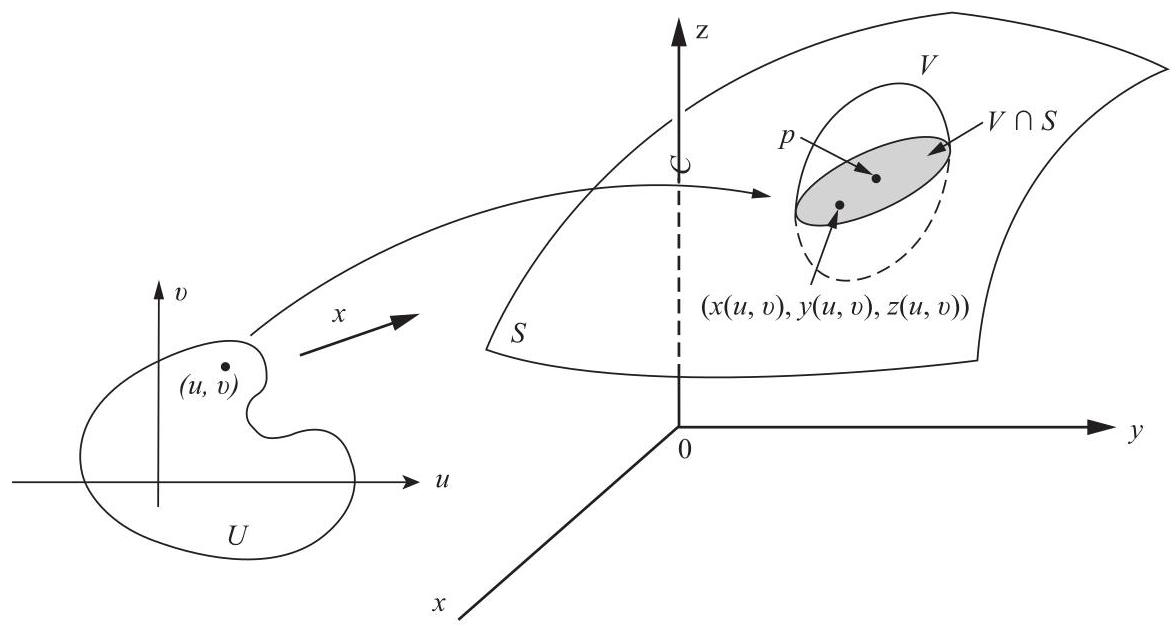
\includegraphics[max width=1.0\textwidth]{images/bo_d4b9jf3ef24c73e0334g_65_180_1151_1176_633_0.jpg}
\end{center}
\hspace*{3em} 

图 2-1

1. \(\mathbf{x}\) 是可微的.这意味着如果我们写出

\[
\mathbf{x}\left( {\mathrm{u},\mathrm{v}}\right)  = \left( {x\left( {\mathrm{u},\mathrm{v}}\right) ,\mathrm{y}\left( {\mathrm{u},\mathrm{v}}\right) ,\mathrm{z}\left( {\mathrm{u},\mathrm{v}}\right) }\right) ,\;\left( {\mathrm{u},\mathrm{v}}\right)  \in  \mathrm{U},
\]

函数 \(x\left( {\mathrm{u},\mathrm{v}}\right) ,\mathrm{y}\left( {\mathrm{u},\mathrm{v}}\right) ,\mathrm{z}\left( {\mathrm{u},\mathrm{v}}\right)\) 在 \(\mathrm{U}\) 中具有所有阶的连续偏导数.



† 本节中的证明在初读时可以省略.



2. \(\mathbf{x}\) 是一个同胚.由于根据条件 1， \(\mathbf{x}\) 是连续的，这意味着 \(\mathbf{x}\) 存在一个连续的逆映射 \({\mathbf{x}}^{-1} : \mathrm{V} \cap  S \rightarrow  \mathrm{U}\) .

3.(正则性条件.)对于每个 \(\mathrm{q} \in  \mathrm{U}\) ，微分 \({\mathrm{{dx}}}_{\mathrm{q}}\) : \({\mathbb{R}}^{2} \rightarrow  {\mathbb{R}}^{3}\) 是单射. \({}^{ \dagger  }\)

我们将在稍后解释条件 3.

映射 \(\mathbf{x}\) 被称为参数化或(局部)坐标系(在 \(p\) 的一个邻域中). \(S\) 中的 \(p\) 的邻域 \(V \cap  S\) 被称为坐标邻域.

为了使条件 3 具有更熟悉的形式，让我们计算线性映射 \(d{\mathbf{x}}_{q}\) 在 \({R}^{2}\) 的标准基 \({e}_{1} = \left( {1,0}\right) ,{e}_{2} = \left( {0,1}\right)\) (具有坐标 \(\left( {u,v}\right)\) )和 \({R}^{3}\) 的标准基 \({f}_{1} = \left( {1,0,0}\right) ,{f}_{2} = \left( {0,1,0}\right) ,{f}_{3} = \left( {0,0,1}\right)\) (具有坐标 \(\left( {x,y,z}\right)\) )下的矩阵.

设 \(q = \left( {{u}_{0},{v}_{0}}\right)\) .向量 \({e}_{1}\) 是曲线 \(u \rightarrow  \left( {u,{v}_{0}}\right)\) 的切向量，该曲线在 \(\mathbf{x}\) 下的像是一条曲线

\[
u \rightarrow  \left( {x\left( {u,{v}_{0}}\right) ,y\left( {u,{v}_{0}}\right) ,z\left( {u,{v}_{0}}\right) }\right) .
\]

这个像曲线(称为坐标曲线 \(v = {v}_{0}\) )位于 \(S\) 上，并在 \(\mathbf{x}\left( q\right)\) 处具有切向量(图 2-2)

\[
\left( {\frac{\partial x}{\partial u},\frac{\partial y}{\partial u},\frac{\partial z}{\partial u}}\right)  = \frac{\partial \mathbf{x}}{\partial u},
\]

\begin{center}
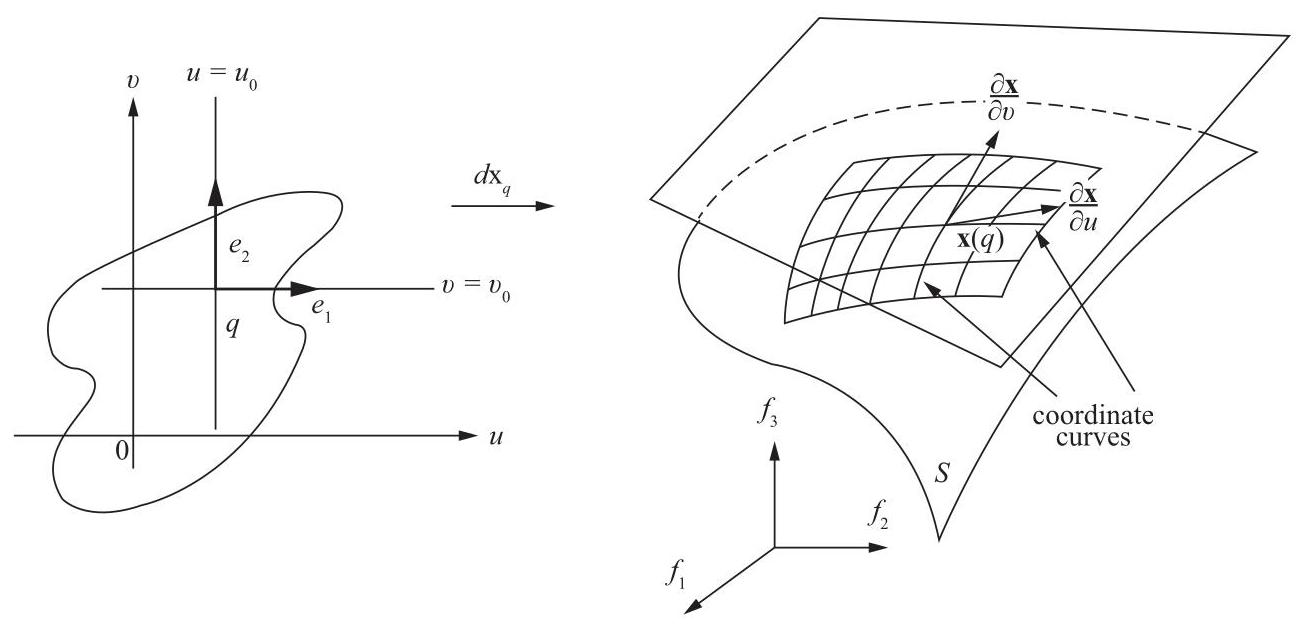
\includegraphics[max width=1.0\textwidth]{images/bo_d4b9jf3ef24c73e0334g_66_195_1269_1302_625_0.jpg}
\end{center}
\hspace*{3em} 

图 2-2



在斜体上下文中，字母符号为罗马体，以便与周围文本区分.



其中导数在 \(\left( {{u}_{0},{v}_{0}}\right)\) 处计算，向量由其在基 \(\left\{  {{f}_{1},{f}_{2},{f}_{3}}\right\}\) 中的分量表示.根据微分的定义(第 2 章附录，定义 1)，

\[
d{\mathbf{x}}_{q}\left( {e}_{1}\right) \left( {\frac{\partial x}{\partial u},\frac{\partial y}{\partial u},\frac{\partial z}{\partial u}}\right)  = \frac{\partial \mathbf{x}}{\partial u}.
\]

类似地，使用坐标曲线 \(u = {u}_{0}\) (由曲线 \(v \rightarrow  \left( {{u}_{0},v}\right) )\) 的映射 \(\mathbf{x}\) 得到)，我们得到

\[
d{\mathbf{x}}_{q}\left( {e}_{2}\right)  = \left( {\frac{\partial x}{\partial v},\frac{\partial y}{\partial v},\frac{\partial z}{\partial v}}\right)  = \frac{\partial \mathbf{x}}{\partial v}.
\]

因此，线性映射 \(d{\mathbf{x}}_{q}\) 在所引基下的矩阵为

\[
d{\mathbf{x}}_{q} = \left( \begin{array}{ll} \frac{\partial x}{\partial u} & \frac{\partial x}{\partial v} \\  \frac{\partial y}{\partial u} & \frac{\partial y}{\partial v} \\  \frac{\partial z}{\partial u} & \frac{\partial z}{\partial v} \end{array}\right) .
\]

定义 1 的条件 3 现在可以通过要求该矩阵的两个列向量线性无关来表达；或者，等价地，向量积 \(\partial \mathbf{x}/\partial u \land  \partial \mathbf{x}/\partial v \neq  0\) ；或者，用另一种方式，矩阵 \(d{\mathbf{x}}_{q}\) 的二阶子式之一，即雅可比行列式之一

\[
\frac{\partial \left( {x,y}\right) }{\partial \left( {u,v}\right) } = \left| \begin{array}{ll} \frac{\partial x}{\partial u} & \frac{\partial x}{\partial v} \\  \frac{\partial y}{\partial u} & \frac{\partial y}{\partial v} \end{array}\right| ,\;\frac{\partial \left( {y,z}\right) }{\partial \left( {u,v}\right) },\;\frac{\partial \left( {x,z}\right) }{\partial \left( {u,v}\right) },
\]

在 \(q\) 处不为零.

注 1. 定义 1 值得商榷.首先，与我们在第 1 章中处理曲线的方式不同，我们将曲面定义为 \({R}^{3}\) 的一个子集 \(S\) ，而不是一个映射.这是通过用满足条件 1、2 和 3 的参数化的迹来覆盖 \(S\) 来实现的.

如果我们期望在 \(S\) 上进行微分几何，那么条件 1 是非常自然的.条件 2 中的一对一性是为了防止正则曲面发生自相交.如果我们想讨论，例如，某一点 \(p \in  S\) 处的切平面(见图 2-3(a))，这一点是显然必要的.条件 2 中逆映射的连续性有一个更微妙的目的，只有在下一节中才能完全理解.目前，我们将提到这个条件对于证明某些用参数化定义的对象的定义不依赖于该参数化而仅依赖于集合 \(S\) 本身是至关重要的.最后，正如我们将在 2.4 节中所示，条件 3 将保证在 \(S\) 的所有点都存在一个“切平面”(见图 2-3(b)).

\begin{center}
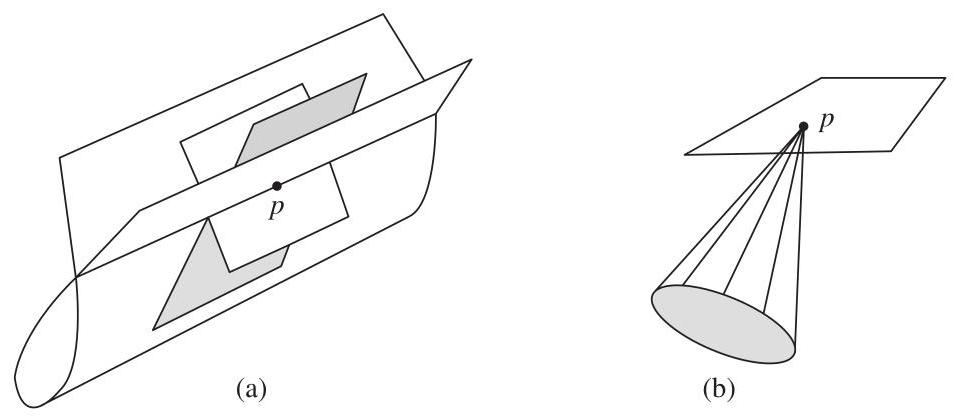
\includegraphics[max width=0.8\textwidth]{images/bo_d4b9jf3ef24c73e0334g_68_303_592_958_416_0.jpg}
\end{center}
\hspace*{3em} 

图 2-3. 在正则曲面定义中应避免的一些情况.

例 1. 让我们证明单位球面

\[
{S}^{2} = \left\{  {\left( {x,y,z}\right)  \in  {R}^{3};{x}^{2} + {y}^{2} + {z}^{2} = 1}\right\}
\]

是一个正则曲面.

我们首先验证由下式给出的映射 \({\mathbf{x}}_{1} : U \subset  {R}^{2} \rightarrow  {R}^{3}\)

\[
{\mathbf{x}}_{1}\left( {x,y}\right)  = \left( {x,y, + \sqrt{1 - \left( {{x}^{2} + {y}^{2}}\right) }}\right) ,\;\left( {x,y}\right)  \in  U,
\]

其中 \({R}^{2} = \left\{  {\left( {x,y,z}\right)  \in  {R}^{3};z = 0}\right\}\) 和 \(U = \left\{  {\left( {x,y}\right)  \in  {R}^{2};{x}^{2} + {y}^{2} < 1}\right\}\) ，是 \({S}^{2}\) 的一个参数化.注意 \({\mathbf{x}}_{1}\left( U\right)\) 是 \({xy}\) 平面上方的 \({S}^{2}\) 的(开放)部分.

由于 \({x}^{2} + {y}^{2} < 1\) ，函数 \(+ \sqrt{1 - \left( {{x}^{2} + {y}^{2}}\right) }\) 具有所有阶的连续偏导数.因此， \({\mathbf{x}}_{1}\) 是可微的，并且条件 1 成立.

条件 3 很容易验证，因为

\[
\frac{\partial \left( {x,y}\right) }{\partial \left( {x,y}\right) } \equiv  1
\]

为检查条件 2，我们观察到 \({\mathbf{x}}_{1}\) 是一一映射，并且 \({\mathbf{x}}_{1}^{-1}\) 是(连续的)投影 \(\pi \left( {x,y,z}\right)  = \left( {x,y}\right)\) 到集合 \({\mathbf{x}}_{1}\left( U\right)\) 上的限制.因此， \({\mathbf{x}}_{1}^{-1}\) 在 \({\mathbf{x}}_{1}\left( U\right)\) 上是连续的.

我们现在将用类似的参数化方法覆盖整个球面，如下所示.我们定义 \({\mathbf{x}}_{2} : U \subset  {R}^{2} \rightarrow  {R}^{3}\) 为

\[
{\mathbf{x}}_{2}\left( {x,y}\right)  = \left( {x,y, - \sqrt{1 - \left( {{x}^{2} + {y}^{2}}\right) }}\right) ,
\]

检查 \({\mathbf{x}}_{2}\) 是一个参数化，并观察到 \({\mathbf{x}}_{1}\left( U\right)  \cup  {\mathbf{x}}_{2}\left( U\right)\) 覆盖了 \({S}^{2}\) 减去赤道的部分

\[
\left\{  {\left( {x,y,z}\right)  \in  {R}^{3};{x}^{2} + {y}^{2} = 1,z = 0}\right\}  .
\]

然后，利用 \({xz}\) 和 \({zy}\) 平面，我们定义了参数化

\[
{\mathbf{x}}_{3}\left( {x,z}\right)  = \left( {x, + \sqrt{1 - \left( {{x}^{2} + {z}^{2}}\right) },z}\right)
\]

\[
{\mathbf{x}}_{4}\left( {x,z}\right)  = \left( {x, - \sqrt{1 - \left( {{x}^{2} + {z}^{2}}\right) },z}\right)
\]

\[
{\mathbf{x}}_{5}\left( {y,z}\right)  = \left( {+\sqrt{1 - \left( {{y}^{2} + {z}^{2}}\right) },y,z}\right) ,
\]

\[
{\mathbf{x}}_{6}\left( {y,z}\right)  = \left( {-\sqrt{1 - \left( {{y}^{2} + {z}^{2}}\right) },y,z}\right) ,
\]

它们与 \({\mathbf{x}}_{1}\) 和 \({\mathbf{x}}_{2}\) 一起，完全覆盖了 \({S}^{2}\) (图 2-4)，并表明 \({S}^{2}\) 是一个正则曲面.

\begin{center}
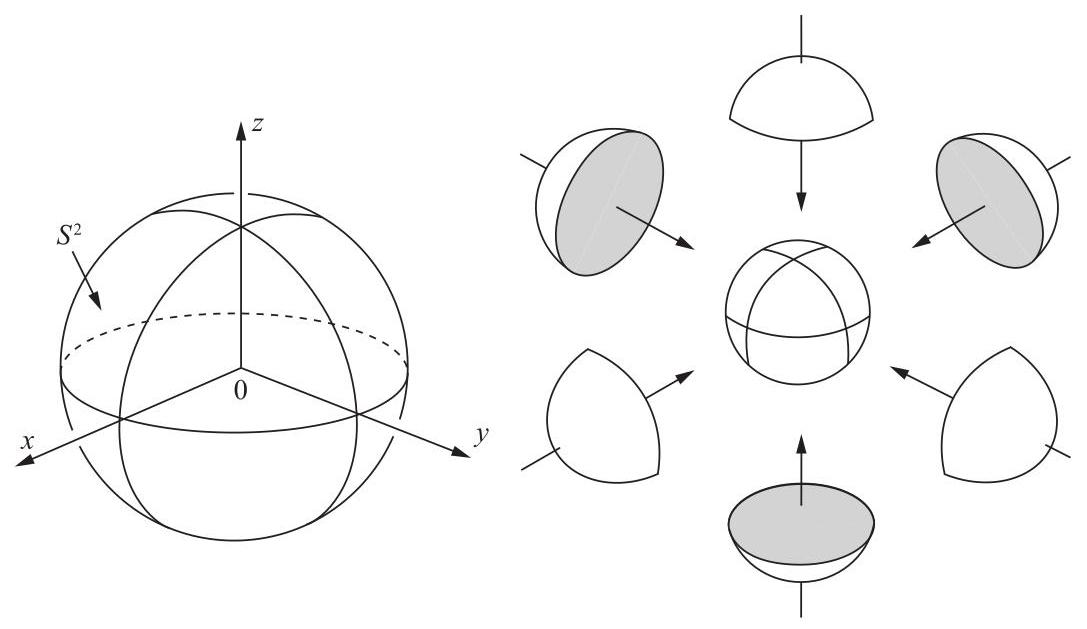
\includegraphics[max width=0.9\textwidth]{images/bo_d4b9jf3ef24c73e0334g_69_224_1131_1087_629_0.jpg}
\end{center}
\hspace*{3em} 

图 2-4

对于大多数应用，将参数化与 \({S}^{2}\) 上的地理坐标相关联是方便的.令 \(V = \{ \left( {\theta ,\varphi }\right) ;0 < \theta  < \pi ,0 < \varphi  < {2\pi }\}\) ，并令 \(\mathbf{x} : V \rightarrow  {R}^{3}\) 由下式给出

\[
\mathbf{x}\left( {\theta ,\varphi }\right)  = \left( {\sin \theta \cos \varphi ,\sin \theta \sin \varphi ,\cos \theta }\right) .
\]

\begin{center}
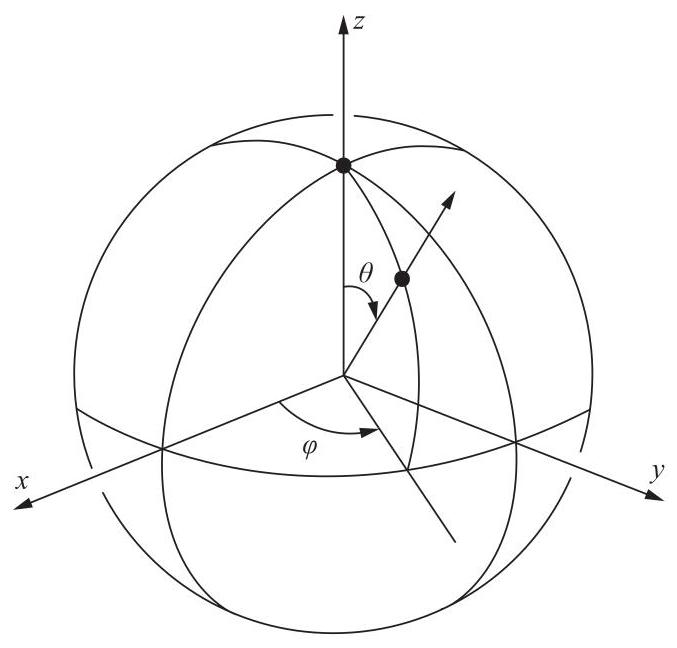
\includegraphics[max width=0.6\textwidth]{images/bo_d4b9jf3ef24c73e0334g_70_196_201_677_648_0.jpg}
\end{center}
\hspace*{3em} 

图 2-5

显然， \(\mathbf{x}\left( V\right)  \subset  {S}^{2}\) .我们将证明 \(\mathbf{x}\) 是 \({S}^{2}.\theta\) 的参数化，通常称为余纬度(纬度的补角)， \(\varphi\) 是经度(图 2-5).

显然，函数 \(\sin \theta \cos \varphi ,\sin \theta \sin \varphi ,\cos \theta\) 具有所有阶的连续偏导数；因此， \(\mathbf{x}\) 是可微的.此外，为了使雅可比行列式

\[
\frac{\partial \left( {x,y}\right) }{\partial \left( {\theta ,\varphi }\right) } = \cos \theta \sin \theta
\]

\[
\frac{\partial \left( {y,z}\right) }{\partial \left( {\theta ,\varphi }\right) } = {\sin }^{2}\theta \cos \varphi
\]

\[
\frac{\partial \left( {x,z}\right) }{\partial \left( {\theta ,\varphi }\right) } =  - {\sin }^{2}\theta \sin \varphi
\]

同时消失，必须满足

\[
{\cos }^{2}\theta {\sin }^{2}\theta  + {\sin }^{4}\theta {\cos }^{2}\varphi  + {\sin }^{4}\theta {\sin }^{2}\varphi  = {\sin }^{2}\theta  = 0.
\]

这在 \(V\) 中不会发生，因此定义 1 的条件 1 和 3 得到满足.

接下来，我们观察到给定 \(\left( {x,y,z}\right)  \in  {S}^{2} - C\) ，其中 \(C\) 是半圆

\[
C = \left\{  {\left( {x,y,z}\right)  \in  {S}^{2};y = 0,x \geq  0}\right\}  ,
\]

\(\theta\) 由 \(\theta  = {\cos }^{-1}z\) 唯一确定，因为 \(0 < \theta  < \pi\) .通过知道 \(\theta\) ，我们从 \(x = \sin \theta \cos \varphi ,y = \sin \theta \sin \varphi\) 中找到 \(\sin \varphi\) 和 \(\cos \varphi\) ，这就唯一确定了 \(\varphi\)  \(\left( {0 < \varphi  < {2\pi }}\right)\) .因此， \(\mathbf{x}\) 有一个逆 \({\mathbf{x}}^{-1}\) .为了完成条件 2 的验证，我们应该证明 \({\mathbf{x}}^{-1}\) 是连续的.然而，由于我们很快将证明(命题 4)只要我们已经知道集合 \(S\) 是一个正则曲面，这个验证就不是必需的，所以我们在这里不进行.

我们注意到 \(\mathbf{x}\left( V\right)\) 只省略了 \({S}^{2}\) 的一个半圆(包括两个极点)，并且 \({S}^{2}\) 可以用两种此类参数化的坐标邻域来覆盖.

在练习 16 中，我们将说明如何用另一组有用的坐标邻域覆盖 \({S}^{2}\) .

示例 1 表明，直接根据定义判断给定的 \({R}^{3}\) 的子集是否为正则曲面可能相当繁琐.在进行更多示例之前，我们将介绍两个将简化此任务的命题.命题 1 显示了正则曲面的定义与函数 \(z = f\left( {x,y}\right)\) 的图之间的关系.命题 2 使用反函数定理，并将正则曲面的定义与形式为 \(f\left( {x,y,z}\right)  =\) 常量的子集相关联.

命题 1. 如果 \(\mathrm{f} : \mathrm{U} \rightarrow  \mathbb{R}\) 在 \({\mathbb{R}}^{2}\) 的开集 \(\mathrm{U}\) 中是可微函数，则 \(\mathrm{f}\) 的图，即 \({\mathbb{R}}^{3}\) 中由 \(\left( {x,\mathrm{y},\mathrm{f}\left( {x,\mathrm{y}}\right) }\right)\) 给出的子集，对于 \(\left( {x,\mathrm{y}}\right)  \in  \mathrm{U}\) ，是一个正则曲面.

证明.只需证明映射 \(\mathbf{x} : U \rightarrow  {R}^{3}\) 由下式给出

\[
\mathbf{x}\left( {u,v}\right)  = \left( {u,v,f\left( {u,v}\right) }\right)
\]

是该图像的一个参数化，其坐标邻域覆盖了图像的每个点.条件 1 显然满足，条件 3 也不难满足，因为 \(\partial \left( {x,y}\right) /\partial \left( {u,v}\right)  \equiv  1\) .最后，图像上的每个点 \(\left( {x,y,z}\right)\) 是唯一的点 \(\left( {u,v}\right)  = \left( {x,y}\right)  \in  U.\mathbf{x}\) 在 \(\mathbf{x}\) 下的像，因此是一一对应的.并且由于 \({\mathbf{x}}^{-1}\) 是 \(f\) 在图像上的限制，即 \({R}^{3}\) 到 \({xy}\) 平面的(连续)投影，所以 \({\mathbf{x}}^{-1}\) 是连续的.Q.E.D.

在陈述命题 2 之前，我们需要一个定义.

定义 2. 给定一个在 \({\mathbb{R}}^{N}\) 的开集 \(\mathrm{U}\) 中定义的微分映射 \(\mathrm{F} : \mathrm{U} \subset  {\mathbb{R}}^{N} \rightarrow  {\mathbb{R}}^{\mathrm{m}}\) ，如果微分 \({\mathrm{{dF}}}_{\mathrm{p}} : {\mathbb{R}}^{N} \rightarrow  {\mathbb{R}}^{\mathrm{m}}\) 不是一个满射(或映上)映射，则称 \(\mathrm{p} \in  \mathrm{U}\) 是 \(\mathrm{F}\) 的一个临界点.临界点 \(\mathrm{F}\left( \mathrm{p}\right)  \in  {\mathbb{R}}^{\mathrm{m}}\) 的像称为 \(\mathrm{F}\) 的一个临界值. \({\mathbb{R}}^{\mathrm{m}}\) 中不是临界值的点称为 \(\mathrm{F}\) 的一个正则值.

这种术语显然是针对 \(f : U \subset  R \rightarrow  R\) 是实变量的实值函数这一特殊情况而提出的.如果 \({f}^{\prime }\left( {x}_{0}\right)  = 0\) ，即微分 \(d{f}_{{x}_{0}}\) 将 \(R\) 中的所有向量映射到零向量(图 2-6)，则点 \({x}_{0} \in  U\) 是临界的.请注意，任何点 \(a \notin  f\left( U\right)\) 都是 \(f\) 的一个平凡正则值.

如果 \(f : U \subset  {R}^{3} \rightarrow  R\) 是一个可微函数，那么 \(d{f}_{p}\) 应用于向量 \(\left( {1,0,0}\right)\) 是通过计算曲线在 \(f\left( p\right)\) 处的切向量得到的

\[
x \rightarrow  f\left( {x,{y}_{0},{z}_{0}}\right) .
\]

\begin{center}
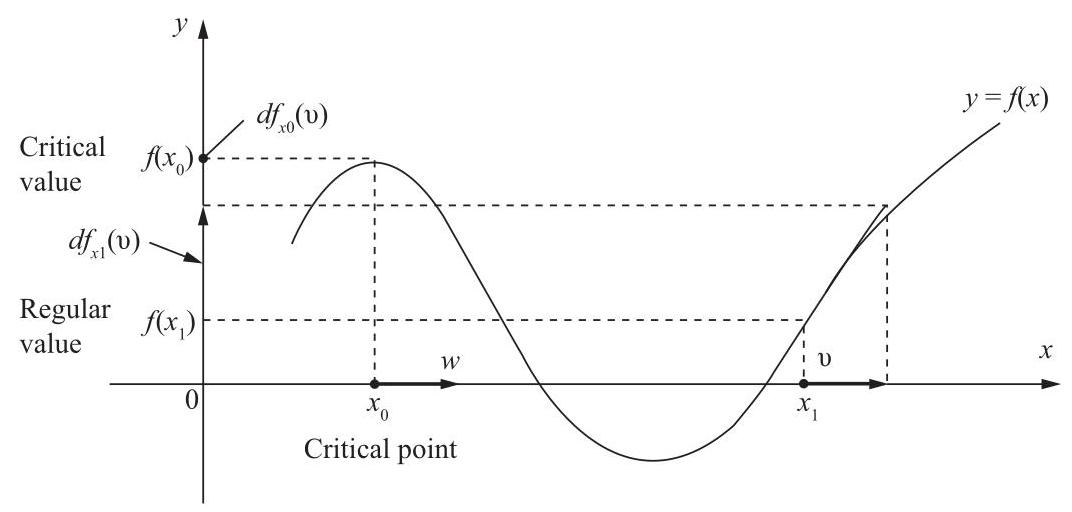
\includegraphics[max width=0.9\textwidth]{images/bo_d4b9jf3ef24c73e0334g_72_247_198_1072_512_0.jpg}
\end{center}
\hspace*{3em} 

图 2-6

由此得出

\[
d{f}_{p}\left( {1,0,0}\right)  = \frac{\partial f}{\partial x}\left( {{x}_{0},{y}_{0},{z}_{0}}\right)  = {f}_{x}
\]

同理可得

\[
d{f}_{p}\left( {0,1,0}\right)  = {f}_{y},\;d{f}_{p}\left( {0,0,1}\right)  = {f}_{z}.
\]

我们得出结论，在基 \(\left( {1,0,0}\right) ,\left( {0,1,0}\right) ,\left( {0,0,1}\right)\) 下 \(d{f}_{p}\) 的矩阵由下式给出

\[
d{f}_{p} = \left( {{f}_{x},{f}_{y},{f}_{z}}\right) .
\]

在这种情况下，请注意，说 \(d{f}_{p}\) 不是满射等价于说 \({f}_{x} = {f}_{y} = {f}_{z} = 0\) 在 \(p\) 处.因此， \(a \in  f\left( U\right)\) 是 \(f : U \subset  {R}^{3} \rightarrow  R\) 的一个正则值当且仅当 \({f}_{x},{f}_{y}\) 和 \({f}_{z}\) 在逆像的任何点处不同时为零

\[
{f}^{-1}\left( a\right)  = \{ \left( {x,y,z}\right)  \in  U : f\left( {x,y,z}\right)  = a\} .
\]

命题 2. 如果 \(\mathrm{f} : \mathrm{U} \subset  {\mathbb{R}}^{3} \rightarrow  \mathbb{R}\) 是一个可微函数，并且 \(\mathrm{a} \in  \mathrm{f}\left( \mathrm{U}\right)\) 是 \(\mathrm{f}\) 的一个正则值，那么 \({\mathrm{f}}^{-1}\left( \mathrm{a}\right)\) 是 \({R}^{3}\) 中的一个正则曲面.

证明. 设 \(p = \left( {{x}_{0},{y}_{0},{z}_{0}}\right)\) 是 \({f}^{-1}\left( a\right)\) 中的一个点. 因为 \(a\) 是 \(f\) 的一个正则值，所以我们可以假设，如果需要的话，通过重命名坐标轴，使得 \({f}_{z} \neq  0\) 在 \(p\) 处成立. 我们定义一个映射 \(F : U \subset  {R}^{3} \rightarrow  {R}^{3}\) 如下:

\[
F\left( {x,y,z}\right)  = \left( {x,y,f\left( {x,y,z}\right) }\right) ,
\]

并且我们用 \(\left( {u,v,t}\right)\) 表示 \({R}^{3}\) 中 \(F\) 取值的点的坐标. \(F\) 在 \(p\) 处的微分由下式给出:

\[
d{F}_{p} = \left( \begin{matrix} 1 & 0 & 0 \\  0 & 1 & 0 \\  {f}_{x} & {f}_{y} & {f}_{z} \end{matrix}\right) ,
\]

由此可得

\[
\det \left( {d{F}_{p}}\right)  = {f}_{z} \neq  0.
\]

因此，我们可以应用反函数定理(参见第 2 章附录)，该定理保证存在 \(p\) 的邻域 \(V\) 和 \(F\left( p\right)\) 的邻域 \(W\) ，使得 \(F : V \rightarrow  W\) 可逆且逆映射 \({F}^{-1} : W \rightarrow  V\) 可微(图 2-7).由此可知， \({F}^{-1}\) 的坐标函数，即函数

\[
x = u,\;y = v,\;z = g\left( {u,v,t}\right) ,\;\left( {u,v,t}\right)  \in  W,
\]

是可微的. 特别地， \(z = g\left( {u,v,a}\right)  = h\left( {x,y}\right)\) 是一个定义在 \(V\) 到 \({xy}\) 平面的投影上的可微函数. 因为

\[
F\left( {{f}^{-1}\left( a\right)  \cap  V}\right)  = W \cap  \{ \left( {u,v,t}\right) ;t = a\} ,
\]

\begin{center}
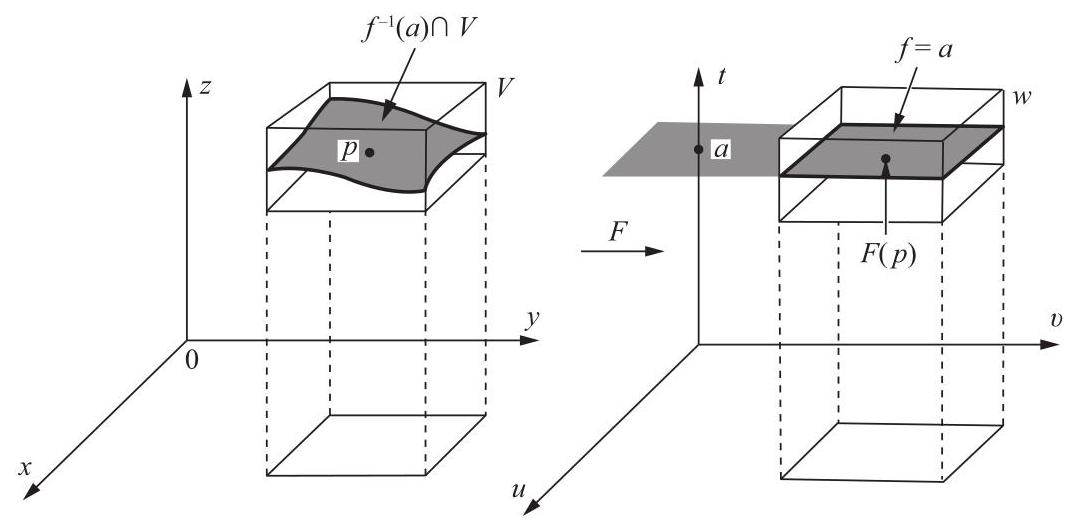
\includegraphics[max width=0.9\textwidth]{images/bo_d4b9jf3ef24c73e0334g_73_226_1108_1077_526_0.jpg}
\end{center}
\hspace*{3em} 

图 2-7

我们得出 \(h\) 的图像是 \({f}^{-1}\left( a\right)  \cap  V\) . 根据命题 \(1,{f}^{-1}\left( a\right)  \cap  V\) 是 \(p\) 的一个坐标邻域. 因此，每个 \(p \in  {f}^{-1}\left( a\right)\) 都可以被一个坐标邻域覆盖，所以 \({f}^{-1}\left( a\right)\) 是一个正则曲面. 证毕.

注 2. 证明本质上是使用反函数定理“求解”方程 \(f\left( {x,y,z}\right)  = a\) 中的 \(z\) ，如果 \({f}_{z}\left( p\right)  \neq  0\) ，则可以在 \(p\) 的邻域中完成. 这个事实是通用隐函数定理的一个特例，它源于反函数定理，并且实际上等价于反函数定理.

例 2. 椭球体

\[
\frac{{x}^{2}}{{a}^{2}} + \frac{{y}^{2}}{{b}^{2}} + \frac{{z}^{2}}{{c}^{2}} = 1
\]

是一个正则曲面. 事实上，它是 \({f}^{-1}\left( 0\right)\) 的集合，其中

\[
f\left( {x,y,z}\right)  = \frac{{x}^{2}}{{a}^{2}} + \frac{{y}^{2}}{{b}^{2}} + \frac{{z}^{2}}{{c}^{2}} - 1
\]

是一个可微函数，并且 0 是 \(f\) 的一个正则值. 这是因为偏导数 \({f}_{x} = {2x}/{a}^{2},{f}_{y} = {2y}/{b}^{2},{f}_{z} = {2z}/{c}^{2}\) 同时只在点 \(\left( {0,0,0}\right)\) 处消失，而该点不属于 \({f}^{-1}\left( 0\right)\) . 这个例子包括球体作为 \(\left( {a = b = c = 1}\right)\) 的一个特例.

到目前为止介绍的正则曲面例子都是 \({R}^{3}\) 的连通子集. 如果曲面 \(S \subset  {R}^{3}\) 的任意两点都可以通过 \(S\) 中的连续曲线连接，则称该曲面是连通的. 在正则曲面的定义中，我们没有对曲面的连通性做任何限制，下面的例子表明命题 2 给出的正则曲面可能不是连通的.

示例 3. 双叶双曲面 \(- {x}^{2} - {y}^{2} + {z}^{2} = 1\) 是一个正则曲面，因为它可以由 \(S = {f}^{-1}\left( 0\right)\) 给出，其中 0 是 \(f\left( {x,y,z}\right)  =  - {x}^{2} - {y}^{2} + {z}^{2} - 1\) 的一个正则值(图 2-8).注意曲面 \(S\) 是不连通的；也就是说，给定两个位于两个不同片 \(\left( {z > 0\text{ and }z < 0}\right)\) 中的点，不可能用一个包含在该曲面内的连续曲线 \(\alpha \left( t\right)  = \left( {x\left( t\right) ,y\left( t\right) ,z\left( t\right) }\right)\) 将它们连接起来；否则， \(z\) 会改变符号，并且对于某个 \({t}_{0}\) ，我们有 \(z\left( {t}_{0}\right)  = 0\) ，这意味着 \(\alpha \left( {t}_{0}\right)  \notin  S\) .

顺便说一句，示例 3 的论证可用于证明一个连通曲面的性质，我们将反复使用该性质.如果 \(\mathrm{f} : S \subset  {\mathbb{R}}^{3} \rightarrow  \mathbb{R}\) 是定义在连通曲面 \(S\) 上的一个非零连续函数，那么 \(\mathrm{f}\) 在 \(S\) 上不改变符号.

为了证明这一点，我们使用中间值定理(附录第 2 章，命题 4).假设，通过反证法，对于某些点 \(p,q \in  S\) ，我们有 \(f\left( p\right)  > 0\) 和 \(f\left( q\right)  < 0\) .由于 \(S\) 是连通的，存在一条连续曲线 \(\alpha  : \left\lbrack  {a,b}\right\rbrack   \rightarrow  S\) ，使得 \(\alpha \left( a\right)  = p,\alpha \left( b\right)  = q\) .通过将中间值定理应用于连续函数 \(f \circ  \alpha  : \left\lbrack  {a,b}\right\rbrack   \rightarrow  R\) ，我们发现存在 \(c \in  \left( {a,b}\right)\) ，使得 \(f \circ  \alpha \left( c\right)  = 0\) ；也就是说， \(f\) 在 \(\alpha \left( c\right)\) 处为零，这与假设矛盾.

\begin{center}
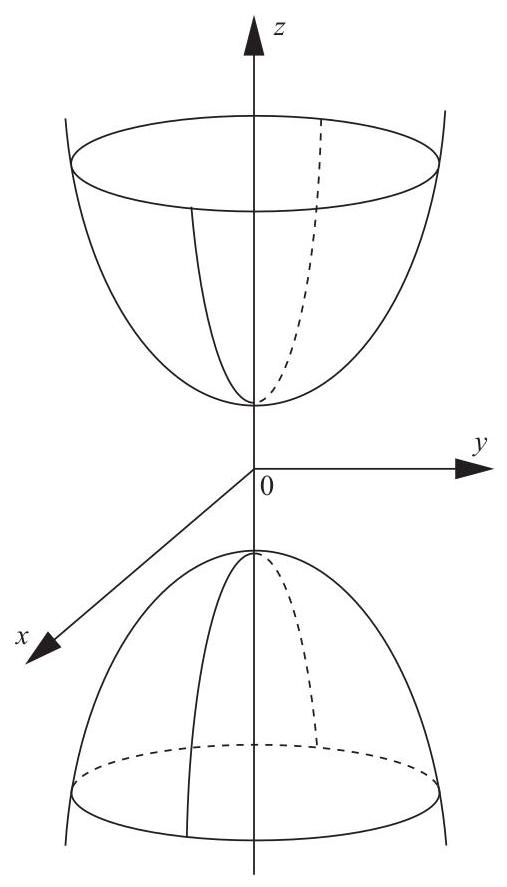
\includegraphics[max width=0.4\textwidth]{images/bo_d4b9jf3ef24c73e0334g_75_177_195_507_887_0.jpg}
\end{center}
\hspace*{3em} 

图 2-8. 一个不连通的曲面: \(- {y}^{2} - {x}^{2} + {z}^{2} = 1\)

示例 4. 圆环面 \(T\) 是由一个半径为 \(r\) 的圆 \({S}^{1}\) 绕着一个位于该圆平面内且与圆心距离为 \(a > r\) 的直线旋转而生成的“曲面”(图 2-9).

\begin{center}
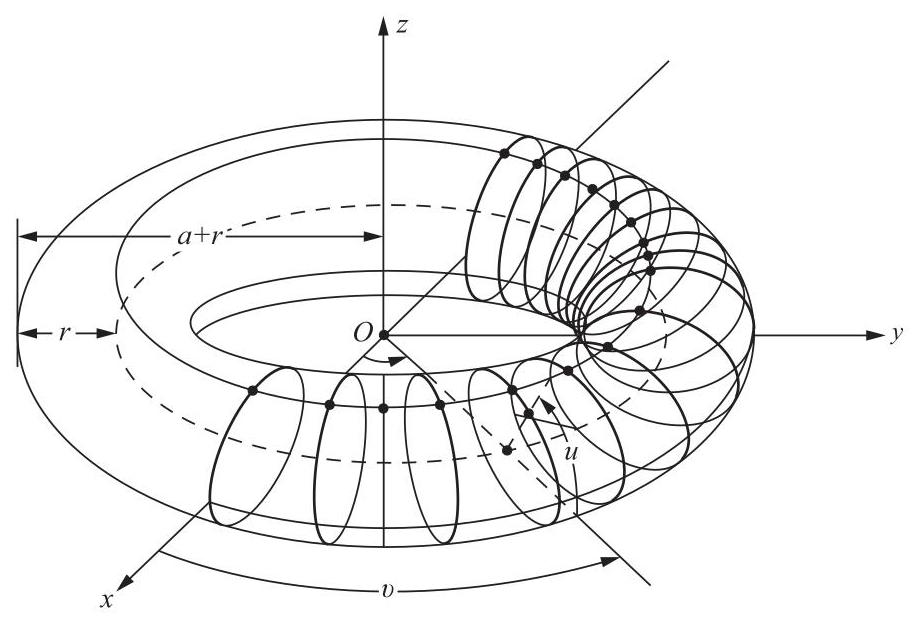
\includegraphics[max width=0.8\textwidth]{images/bo_d4b9jf3ef24c73e0334g_75_307_1403_917_619_0.jpg}
\end{center}
\hspace*{3em} 

图 2-9

设 \({S}^{1}\) 是 \({yz}\) 平面中的圆，其圆心在点 \(\left( {0,a,0}\right)\) .那么 \({S}^{1}\) 由 \({\left( y - a\right) }^{2} + {z}^{2} = {r}^{2}\) 给出，并且通过绕 \(z\) 轴旋转该圆得到的图形 \(T\) 的点满足方程

\[
{z}^{2} = {r}^{2} - {\left( \sqrt{{x}^{2} + {y}^{2}} - a\right) }^{2}.
\]

因此， \(T\) 是函数 \({r}^{2}\) 的逆像

\[
f\left( {x,y,z}\right)  = {z}^{2} + {\left( \sqrt{{x}^{2} + {y}^{2}} - a\right) }^{2}.
\]

该函数对于 \(\left( {x,y}\right)  \neq  \left( {0,0}\right)\) 是可微的，并且由于

\[
\frac{\partial f}{\partial z} = {2z},\;\frac{\partial f}{\partial y} = \frac{{2y}\left( {\sqrt{{x}^{2} + {y}^{2}} - a}\right) }{\sqrt{{x}^{2} + {y}^{2}}},
\]

\[
\frac{\partial f}{\partial x} = \frac{{2x}\left( {\sqrt{{x}^{2} + {y}^{2}} - a}\right) }{\sqrt{{x}^{2} + {y}^{2}}},
\]

\({r}^{2}\) 是 \(f\) 的一个正则值.由此可知，圆环面 \(T\) 是一个正则曲面.

命题 1 说可微函数的图像是一个正则曲面.下面的命题提供了这个命题的局部逆命题；也就是说，任何正则曲面在局部上都是一个可微函数的图像.

命题 3. 设 \(S \subset  {\mathbb{R}}^{3}\) 为一个正则曲面，且 \(\mathrm{p} \in  S\) .则存在 \(S\) 中 \(\mathrm{p}\) 的一个邻域 \(\mathrm{V}\) ，使得 \(\mathrm{V}\) 是一个可微函数的图像，该函数具有以下三种形式之一: \(\mathrm{z} = \mathrm{f}\left( {x,\mathrm{y}}\right)\) ， \(\mathrm{y} = \mathrm{g}\left( {x,\mathrm{z}}\right) ,x = \mathrm{h}\left( {\mathrm{y},\mathrm{z}}\right) .\)

证明. 设 \(\mathbf{x} : U \subset  {R}^{2} \rightarrow  S\) 是 \(p\) 中 \(S\) 的一个参数化，并写出 \(\mathbf{x}\left( {u,v}\right)  = \left( {x\left( {u,v}\right) ,y\left( {u,v}\right) ,z\left( {u,v}\right) }\right) ,\left( {u,v}\right)  \in  U\) .根据定义 1 的条件 3，雅可比行列式之一

\[
\frac{\partial \left( {x,y}\right) }{\partial \left( {u,v}\right) },\;\frac{\partial \left( {y,z}\right) }{\partial \left( {u,v}\right) },\;\frac{\partial \left( {z,x}\right) }{\partial \left( {u,v}\right) }
\]

在 \({\mathbf{x}}^{-1}\left( p\right)  = q\) 处不为零.

首先假设 \(\left( {\partial \left( {x,y}\right) /\partial \left( {u,v}\right) }\right) \left( q\right)  \neq  0\) ，并考虑映射 \(\pi  \circ  \mathbf{x}\) : \(U \rightarrow  {R}^{2}\) ，其中 \(\pi\) 是投影 \(\pi \left( {x,y,z}\right)  = \left( {x,y}\right)\) .则 \(\pi  \circ  \mathbf{x}\left( {u,v}\right)  = \; \left( {x\left( {u,v}\right) ,y\left( {u,v}\right) }\right)\) ，并且由于 \(\left( {\partial \left( {x,y}\right) /\partial \left( {u,v}\right) }\right) \left( q\right)  \neq  0\) ，我们可以应用反函数定理来保证存在 \({V}_{1}\) 的邻域 \(q,{V}_{2}\) 和 \(\pi  \circ  \mathbf{x}\left( q\right)\) ，使得 \(\pi  \circ  \mathbf{x}\) 将 \({V}_{1}\) 同胚地映射到 \({V}_{2}\) (图 2-10).由此可知，限制在 \(\mathbf{x}\left( {V}_{1}\right)  = V\) 上的 \(\pi\) 是单射的，并且存在一个可微的逆映射 \({\left( \pi  \circ  \mathbf{x}\right) }^{-1} : {V}_{2} \rightarrow  {V}_{1}\) .注意到，由于 \(\mathbf{x}\) 是一个同胚映射， \(V\) 是 \(S\) 中 \(p\) 的一个邻域.现在，如果我们用函数 \(\left( {u,v}\right)  \rightarrow \; z\left( {u,v}\right)\) 复合映射 \({\left( \pi  \circ  \mathbf{x}\right) }^{-1} : \left( {x,y}\right)  \rightarrow  \left( {u\left( {x,y}\right) ,v\left( {x,y}\right) }\right)\) ，我们会发现 \(V\) 是可微函数 \(z = \; z\left( {u\left( {x,y}\right) ,v\left( {x,y}\right) }\right)  = f\left( {x,y}\right)\) 的图像，这就解决了第一种情况.

\begin{center}
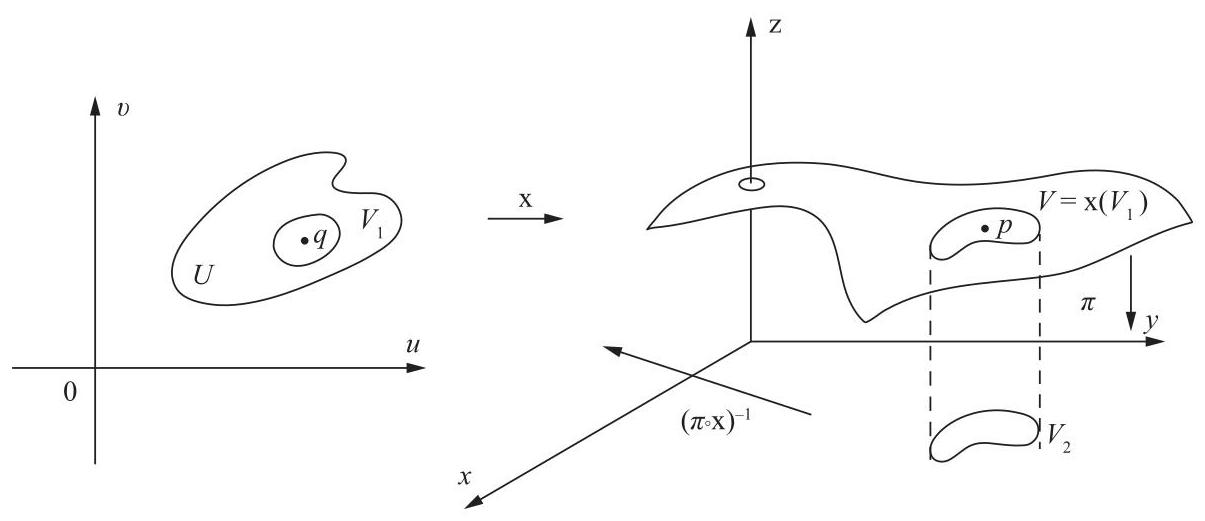
\includegraphics[max width=1.0\textwidth]{images/bo_d4b9jf3ef24c73e0334g_77_180_196_1205_521_0.jpg}
\end{center}
\hspace*{3em} 

图 2-10

其余情况可以以相同的方式处理，得到 \(x = h\left( {y,z}\right)\) 和 \(y = g\left( {x,z}\right)\) .Q.E.D.

下一个命题指出，如果我们已经知道 \(S\) 是一个规则曲面，并且我们有一个参数化的候选 \(\mathbf{x}\) ，那么只要其他条件成立，我们就无需检查 \({\mathbf{x}}^{-1}\) 是否连续.这个说明在示例 1 中使用过.

命题 4. 令 \(\mathrm{p} \in  S\) 为规则曲面 \(S\) 的一个点，令 \(\mathbf{x} : \mathrm{U} \subset  {\mathbb{R}}^{2} \rightarrow  {\mathbb{R}}^{3}\) 为一个映射，其 \(p \in  \mathbf{x}\left( \mathrm{U}\right)  \subset  S\) 满足定义 1 的条件 1 和 3.假设 \(\mathbf{x}\) 是单射的.则 \({\mathbf{x}}^{-1}\) 是连续的.

证明.我们首先采用与命题 3 的证明类似的方法.写出 \(\mathbf{x}\left( {u,v}\right)  = \left( {x\left( {u,v}\right) ,y\left( {u,v}\right) ,z\left( {u,v}\right) }\right) ,\left( {u,v}\right)  \in  U\) ，令 \(q \in  U\) .根据条件 1 和 3，我们可以假设，如果需要，通过交换坐标轴，使得 \(\partial \left( {x,y}\right) /\partial \left( {u,v}\right) \left( q\right)  \neq  0\) .令 \(\pi  : {\mathbb{R}}^{3} \rightarrow  {\mathbb{R}}^{2}\) 为投影 \(\pi \left( {x,y,z}\right)  = \left( {x,y}\right)\) .根据反函数定理，我们在 \(U\) 中的 \(q\) 的邻域 \({V}_{1}\) 和 \({\mathbb{R}}^{2}\) 中的 \(\pi  \circ  \mathbf{x}\left( q\right)\) 的邻域 \({V}_{2}\) 中得到，使得 \(\pi  \circ  \mathbf{x}\) 将 \({V}_{1}\) 同胚地映射到 \({V}_{2}\) .

现在假设 \(\mathbf{x}\) 是双射的.那么，限制在 \(\mathbf{x}\left( {V}_{1}\right) ,{\mathbf{x}}^{-1} = {\left( \pi  \circ  \mathbf{x}\right) }^{-1} \; \circ  \pi\) (图 2.10)上.因此 \({\mathbf{x}}^{-1}\) ，作为连续映射的复合，是连续的.

Q.E.D.

示例 5. 单叶锥 \(C\) ，由下式给出

\[
z =  + \sqrt{{x}^{2} + {y}^{2}},\;\left( {x,y}\right)  \in  {R}^{2},
\]

不是一个规则曲面.请注意，我们不能仅凭“自然”参数化

\[
\left( {x,y}\right)  \rightarrow  \left( {x,y, + \sqrt{{x}^{2} + {y}^{2}}}\right)
\]

不是可微的；可能存在其他满足定义 1 的参数化.

为了证明事实并非如此，我们使用命题 3.如果 \(C\) 是一个规则曲面，那么它将在 \(\left( {0,0,0}\right)  \in  C\) 的邻域内，成为一个具有以下三种形式之一的可微函数的图像: \(y = h\left( {x,z}\right) ,x = g\left( {y,z}\right) ,z = f\left( {x,y}\right)\) .前两种形式可以被排除，因为 \(C\) 在 \({xz}\) 和 \({yz}\) 平面上的投影不是单射的.最后一种形式必须在 \(\left( {0,0,0}\right)\) 的邻域内与 \(z =  + \sqrt{{x}^{2} + {y}^{2}}\) 一致.由于 \(z =  + \sqrt{{x}^{2} + {y}^{2}}\) 在 \(\left( {0,0}\right)\) 处不可微，这是不可能的.

示例 6. 示例 4 中的环面 \(T\) 的一个参数化可以由(图 2-9)给出

\[
\mathbf{x}\left( {u,v}\right)  = \left( {\left( {r\cos u + a}\right) \cos v,\left( {r\cos u + a}\right) \sin v,r\sin u}\right) ,
\]

其中 \(0 < u < {2\pi },0 < v < {2\pi }\) .

定义 1 的条件 1 易于检查，条件 3 归结为一个直接的计算，留作练习.由于我们知道 \(T\) 是一个正则曲面，根据命题 4，条件 2 等价于 \(\mathbf{x}\) 是单射的.

为了证明 \(\mathbf{x}\) 是单射的，我们首先观察到 \(\sin u = z/r\) ；此外，如果 \(\sqrt{{x}^{2} + {y}^{2}} \leq  a\) ，则 \(\pi /2 \leq  u \leq  {3\pi }/2\) ，如果 \(\sqrt{{x}^{2} + {y}^{2}} \geq  a\) ，则 \(0 < u \leq  \pi /2\) 或 \({3\pi }/2 \leq  u < {2\pi }\) .因此，给定 \(\left( {x,y,z}\right)\) ，这唯一确定了 \(u\) ， \(0 < u < {2\pi }\) .通过知道 \(u,x\) 和 \(y\) ，我们找到 \(\cos v\) 和 \(\sin v\) .这唯一确定了 \(v\) ， \(0 < v < {2\pi }\) .因此， \(\mathbf{x}\) 是单射的.

很容易看出，圆环可以被三个这样的坐标邻域覆盖.

\exerciseline

1. 证明圆柱体 \(\left\{  {\left( {x,y,z}\right)  \in  {R}^{3};{x}^{2} + {y}^{2} = 1}\right\}\) 是一个正则曲面，并找到覆盖它的坐标邻域的参数化.

2. 集合 \(\left\{  {\left( {x,y,z}\right)  \in  {R}^{3};z = 0\text{ and }{x}^{2} + {y}^{2} \leq  1}\right\}\) 是一个正则曲面吗？集合 \(\left\{  {\left( {x,y,z}\right)  \in  {R}^{3};z = 0\text{ , and }{x}^{2} + {y}^{2} < 1}\right\}\) 是一个正则曲面吗？

3. 证明顶点在原点的双叶圆锥面，即集合 \(\left\{  {\left( {x,y,z}\right)  \in  {R}^{3};{x}^{2} + {y}^{2} - {z}^{2} = 0}\right\}\) ，不是一个正则曲面.



† 那些在本节中省略了证明的人也应该省略练习 17-19.



4. 令 \(f\left( {x,y,z}\right)  = {z}^{2}\) .证明 0 不是 \(f\) 的正则值，但 \({f}^{-1}\left( 0\right)\) 是一个正则曲面.

*5. 令 \(P = \left\{  {\left( {x,y,z}\right)  \in  {R}^{3};x = y}\right\}\) (一个平面)，令 \(\mathbf{x} : U \subset  {R}^{2} \rightarrow  {R}^{3}\) 由下式给出

\[
\mathbf{x}\left( {u,v}\right)  = \left( {u + v,u + v,{uv}}\right) ,
\]

其中 \(U = \left\{  {\left( {u,v}\right)  \in  {R}^{2};u > v}\right\}\) .显然， \(\mathbf{x}\left( U\right)  \subset  P\) . \(\mathbf{x}\) 是 \(P\) 的参数化吗？

6. 通过将命题 2 应用于 \(h\left( {x,y,z}\right)  = \; f\left( {x,y}\right)  - z.\) 来给出命题 1 的另一个证明.

7. 令 \(f\left( {x,y,z}\right)  = {\left( x + y + z - 1\right) }^{2}\) .

a. 定位 \(f\) 的临界点和临界值.

b. 对于哪些 \(c\) 值，集合 \(f\left( {x,y,z}\right)  = c\) 是一个正则曲面？

c. 对函数 \(f\left( {x,y,z}\right)  = \; {xy}{z}^{2}\) 回答 a 和 b 部分的问题.

8. 令 \(\mathbf{x}\left( {u,v}\right)\) 如定义 1 所示.验证 \(d{\mathbf{x}}_{q} : {R}^{2} \rightarrow  {R}^{3}\) 是单射当且仅当

\[
\frac{\partial \mathbf{x}}{\partial u} \land  \frac{\partial \mathbf{x}}{\partial v} \neq  0
\]

9. 令 \(V\) 为 \({xy}\) 平面上的一个开集.证明集合

\[
\left\{  {\left( {x,y,z}\right)  \in  {R}^{3};z = 0\text{ and }\left( {x,y}\right)  \in  V}\right\}
\]

是一个正则曲面.

10. 令 \(C\) 为 \({xy}\) 平面上的一个“8”字形，令 \(S\) 为 \(C\) 上方的柱面(图 2-11)；即，

\[
S = \left\{  {\left( {x,y,z}\right)  \in  {R}^{3};\left( {x,y}\right)  \in  C}\right\}  .
\]

集合 \(S\) 是一个正则曲面吗？

\begin{center}
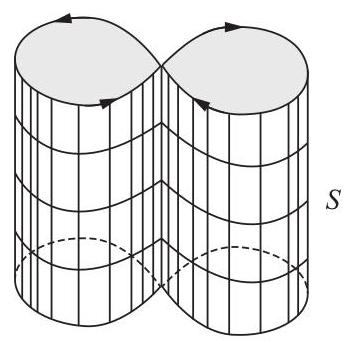
\includegraphics[max width=0.3\textwidth]{images/bo_d4b9jf3ef24c73e0334g_79_178_1763_353_343_0.jpg}
\end{center}
\hspace*{3em} 

图 2-11

11. 证明集合 \(S = \left\{  {\left( {x,y,z}\right)  \in  {R}^{3};z = {x}^{2} - {y}^{2}}\right\}\) 是一个正则曲面，并检查 a 和 b 部分是否为 \(S\) 的参数化:

a. \(\mathbf{x}\left( {u,v}\right)  = \left( {u + v,u - v,{4uv}}\right) ,\left( {u,v}\right)  \in  {R}^{2}\) .

*b. \(\mathbf{x}\left( {u,v}\right)  = \left( {u\cosh v,u\sinh v,{u}^{2}}\right) ,\left( {u,v}\right)  \in  {R}^{2},u \neq  0\) .

这些参数化覆盖了 \(S\) 的哪些部分？

12. 证明由以下公式给出的 \(\mathbf{x} : U \subset  {R}^{2} \rightarrow  {R}^{3}\)

\[
\mathbf{x}\left( {u,v}\right)  = \left( {a\sin u\cos v,b\sin u\sin v,c\cos u}\right) ,\;a,b,c \neq  0,
\]

其中 \(0 < u < \pi ,0 < v < {2\pi }\) 是椭球面

\[
\frac{{x}^{2}}{{a}^{2}} + \frac{{y}^{2}}{{b}^{2}} + \frac{{z}^{2}}{{c}^{2}} = 1
\]

在椭球面上，几何地描述曲线 \(u =\) = const.

*13. 找到双叶双曲面 \(\{ \left( {x,y,z}\right)  \in \; \left. {{R}^{3}; - {x}^{2} - {y}^{2} + {z}^{2} = 1}\right\}\) 的参数化.

14. 半直线 \(\lbrack 0,\infty )\) 垂直于直线 \(E\) ，并从给定的初始位置绕 \(E\) 旋转，同时其原点 0 沿 \(E\) 移动.运动方式是，当 \(\lbrack 0,\infty )\) 旋转角度 \(\theta\) 时，原点与 \(E\) 上初始位置的距离为 \(d = {\sin }^{2}\left( {\theta /2}\right)\) .验证通过移除旋转直线图像中的直线 \(E\) ，我们得到一个正则曲面.如果运动方式是 \(d = \sin \left( {\theta /2}\right)\) ，还需要排除什么才能得到一个正则曲面？

*15. 令两个点 \(p\left( t\right)\) 和 \(q\left( t\right)\) 以相同的速度移动， \(p\) 从 \(\left( {0,0,0}\right)\) 开始沿 \(z\) 轴移动， \(q\) 从 \(\left( {a,0,0}\right) ,a \neq  0\) 开始，并沿 \(y\) 轴平行移动.证明通过 \(p\left( t\right)\) 和 \(q\left( t\right)\) 的直线在 \({R}^{3}\) 中描述了一个由 \(y\left( {x - a}\right)  + {zx} = 0\) 给出的集合.这是一个正则曲面吗？

16. 为球面 \({S}^{2}\) (由 \({x}^{2} + {y}^{2} + {\left( z - 1\right) }^{2} = 1\) 给出)定义一个坐标系的一种方法是考虑所谓的球极投影 \(\pi  : {S}^{2} \sim  \{ N\}  \rightarrow  {R}^{2}\) ，该投影将球面 \({S}^{2}\) 上除北极点 \(N = \left( {0,0,2}\right)\) 之外的点 \(p = \left( {x,y,z}\right)\) 映射到 \({xy}\) 平面与连接 \(N\) 和 \(p\) 的直线的交点上(图 2 - 12).设 \(\left( {u,v}\right)  = \pi \left( {x,y,z}\right)\) ，其中 \(\left( {x,y,z}\right)  \in  {S}^{2} \sim  \{ N\}\) 和 \(\left( {u,v}\right)  \in  {xy}\) 平面.

a. 证明 \({\pi }^{-1} : {R}^{2} \rightarrow  {S}^{2}\) 由下式给出

\[
{\pi }^{-1}\left\{  \begin{array}{l} x = \frac{4u}{{u}^{2} + {v}^{2} + 4}, \\  y = \frac{4v}{{u}^{2} + {v}^{2} + 4}, \\  z = \frac{2\left( {{u}^{2} + {v}^{2}}\right) }{{u}^{2} + {v}^{2} + 4}. \end{array}\right.
\]

\begin{center}
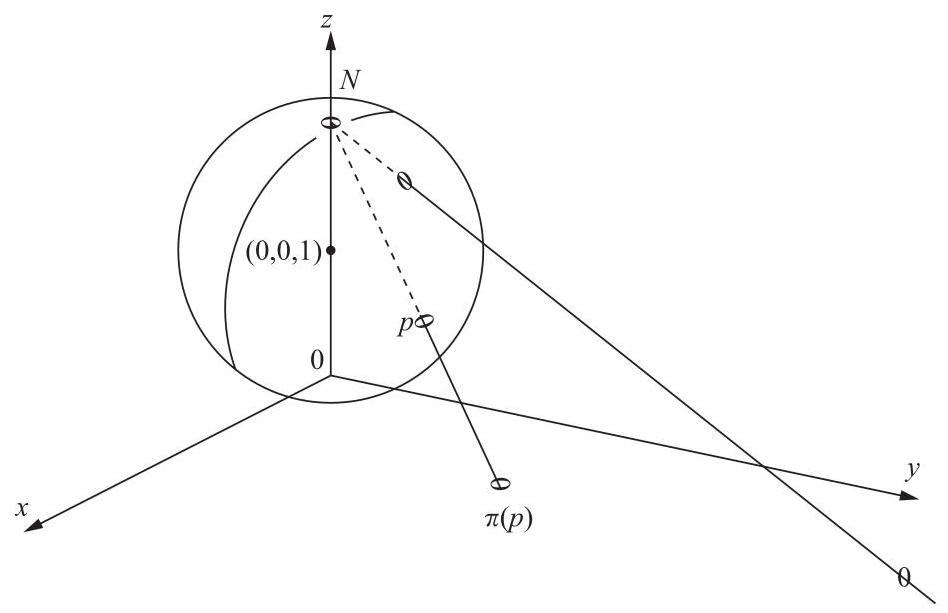
\includegraphics[max width=0.8\textwidth]{images/bo_d4b9jf3ef24c73e0334g_81_289_202_948_613_0.jpg}
\end{center}
\hspace*{3em} 

图 2-12. 球极投影.

b. 证明使用球极投影可以覆盖球面，使其包含两个坐标邻域.

17. 仿照正则曲面定义正则曲线.证明

a. 可微函数的正则值之逆像

\[
f : U \subset  {R}^{2} \rightarrow  R
\]

是一条正则平面曲线.举一个非连通的此类曲线的例子.

b. 可微映射的正则值之逆像

\[
F : U \subset  {R}^{3} \rightarrow  {R}^{2}
\]

是 \({R}^{3}\) 中的一条正则曲线.说明此命题与将 \({R}^{3}\) 中的曲线定义为两个曲面的交集的经典方法之间的关系.

*c. 集合 \(C = \left\{  {\left( {x,y}\right)  \in  {R}^{2};{x}^{2} = {y}^{3}}\right\}\) 不是一条正则曲线.

*18. 假设 \(f\left( {x,y,z}\right)  = u =\) 为常数， \(g\left( {x,y,z}\right)  = v =\) 为常数，

\[
h\left( {x,y,z}\right)  = w = \text{ const. }
\]

描述三族正则曲面，并假设在 \(\left( {{x}_{0},{y}_{0},{z}_{0}}\right)\) 处雅可比行列式

\[
\frac{\partial \left( {f,g,h}\right) }{\partial \left( {x,y,z}\right) } \neq  0.
\]

\begin{center}
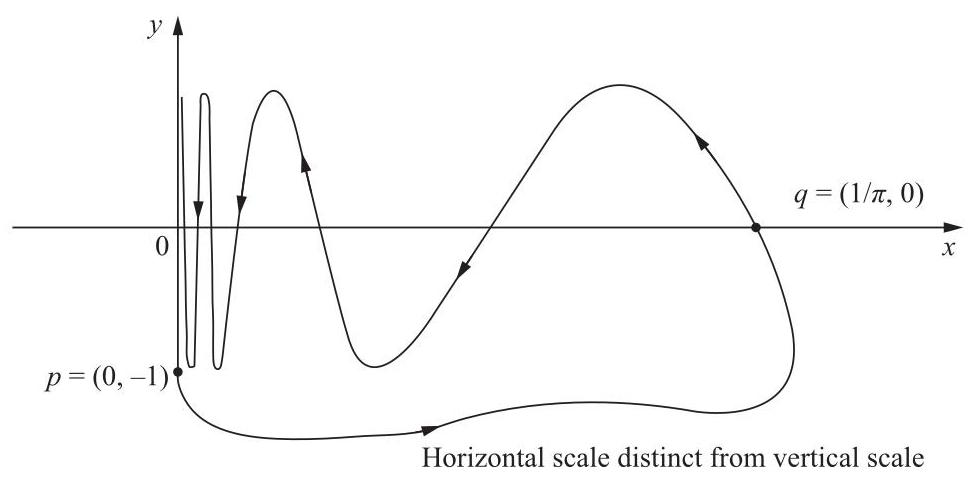
\includegraphics[max width=0.8\textwidth]{images/bo_d4b9jf3ef24c73e0334g_82_299_197_972_479_0.jpg}
\end{center}
\hspace*{3em} 

图 2-13

证明在 \(\left( {{x}_{0},{y}_{0},{z}_{0}}\right)\) 的邻域中，这三个族将由一个从 \({R}^{3}\) 的开集映射到 \({R}^{3}\) 的映射 \(F\left( {u,v,w}\right)  = \left( {x,y,z}\right)\) 来描述，其中族 \(f\left( {x,y,z}\right)  = u\) 的曲面局部参数化，例如，通过在该映射中设置 \(u =\) 为常数来获得.确定三个曲面族的情况下的 \(F\) .

\[
f\left( {x,y,z}\right)  = {x}^{2} + {y}^{2} + {z}^{2} = u = \text{ const.; }\;\text{ (spheres with center }\left( {0,0,0}\right) );
\]

\[
g\left( {x,y,z}\right)  = \frac{y}{x} = v = \text{ const.; }\;\text{ (planes through the }z\text{ axis); }
\]

\[
h\left( {x,y,z}\right)  = \frac{{x}^{2} + {y}^{2}}{{z}^{2}} = w = \text{ const.; }
\]

*19. 令 \(\alpha  : \left( {-3,0}\right)  \rightarrow  {R}^{2}\) 由(图 2-13)定义

\[
\alpha \left( t\right) \left\{  \begin{array}{ll}  = \left( {0, - \left( {t + 2}\right) }\right) , & \text{ if }t \in  \left( {-3, - 1}\right) , \\   = \text{ regular parametrized curve joining }p = \left( {0, - 1}\right) \text{ to }q = \left( {\frac{1}{\pi },0}\right) , & \text{ if }t \in  \left( {-1, - \frac{1}{\pi }}\right) , \\   = \left( {-t,\sin \frac{1}{t}}\right) , & \text{ if }t \in  \left( {-\frac{1}{\pi },0}\right) . \end{array}\right.
\]

可以定义连接 \(p\) 到 \(q\) 的曲线，使得 \(\alpha\) 的所有导数在对应点处连续，并且 \(\alpha\) 没有自交点.令 \(C\) 为 \(\alpha\) 的迹.

a. \(C\) 是正则曲线吗？

b. 令平面 \({R}^{2}\) 的一条法线通过 \(C\) ，从而描述一个“圆柱体” \(S\) . \(S\) 是正则曲面吗？

\section*{2-3. 参数变换；曲面上的可微函数}

微分几何研究曲面在某点邻域内的性质.第 2-2 节中给出的正则曲面定义足以满足此目的.根据此定义，正则曲面上的每一点 \(p\) 都属于一个坐标邻域.此类邻域中的点由其坐标表征，因此我们应该能够用这些坐标来定义我们感兴趣的局部性质.

例如，我们能够定义一个函数 \(f : S \rightarrow  R\) 在正则曲面 \(S\) 的一点 \(p\) 上是否可微是很重要的.一种自然的方法是选择 \(p\) 的一个坐标邻域，其坐标为 \(u,v\) ，并称如果 \(f\) 在坐标 \(u\) 和 \(v\) 下的表达式存在所有阶的连续偏导数，则 \(f\) 在 \(p\) 上是可微的.

然而， \(S\) 的同一点可以属于多个坐标邻域(在第 2-2 节示例 1 的球面上，第一卦限内部的任意一点都属于给定的三个坐标邻域之一).此外，在 \(p\) 的邻域中还可以选择其他的坐标系(球面上提到的点也可以用地理坐标或立体投影参数化；参见第 2-2 节练习 16).为了使上述定义有意义，它必须不依赖于所选的坐标系.换句话说，必须证明当 \(p\) 属于两个坐标邻域，其参数分别为 \(\left( {u,v}\right)\) 和 \(\left( {\xi ,\eta }\right)\) 时，可以通过一个可微变换从一对坐标转换到另一对坐标.

以下命题表明这是正确的.

命题 1 (参数变换).设 \(\mathrm{p}\) 是正则曲面 \(S\) 上的一点，设 \(x : \mathrm{U} \subset  {\mathbb{R}}^{2} \rightarrow  S,\mathrm{y} : \mathrm{V} \subset  {\mathbb{R}}^{2} \rightarrow  S\) 是 \(S\) 的两个参数化，使得 \(\mathrm{p} \in  \mathbf{x}\left( \mathrm{U}\right)  \cap  \mathrm{y}\left( \mathrm{V}\right)  = \mathrm{W}\) .则“坐标变换” \(\mathrm{h} = {\mathbf{x}}^{-1} \circ  \mathbf{y} : {\mathbf{y}}^{-1}\left( \mathrm{\;W}\right)  \rightarrow  {\mathbf{x}}^{-1}\left( \mathrm{\;W}\right)\) (图 2-14) 是一个微分同胚；也就是说， \(\mathrm{h}\) 是可微的，并且存在一个可微的逆映射 \({\mathrm{h}}^{-1}\) .

换句话说，如果 \(\mathbf{x}\) 和 \(\mathbf{y}\) 由下式给出

\[
\mathbf{x}\left( {u,v}\right)  = \left( {x\left( {u,v}\right) ,y\left( {u,v}\right) ,z\left( {u,v}\right) }\right) ,\;\left( {u,v}\right)  \in  U,
\]

\[
\mathbf{y}\left( {\xi ,\eta }\right)  = \left( {x\left( {\xi ,\eta }\right) ,y\left( {\xi ,\eta }\right) ,z\left( {\xi ,\eta }\right) }\right) ,\;\left( {\xi ,\eta }\right)  \in  V,
\]

那么坐标变换 \(h\) ，由下式给出

\[
u = u\left( {\xi ,\eta }\right) ,\;v = v\left( {\xi ,\eta }\right) ,\;\left( {\xi ,\eta }\right)  \in  {\mathbf{y}}^{-1}\left( W\right) ,
\]

具有函数 \(u\) 和 \(v\) 具有所有阶的连续偏导数，并且映射 \(h\) 可以被反转，得到

\[
\xi  = \xi \left( {u,v}\right) ,\;\eta  = \eta \left( {u,v}\right) ,\;\left( {u,v}\right)  \in  {\mathbf{x}}^{-1}\left( W\right) ,
\]



† 本节的证明在初读时可以省略.



\begin{center}
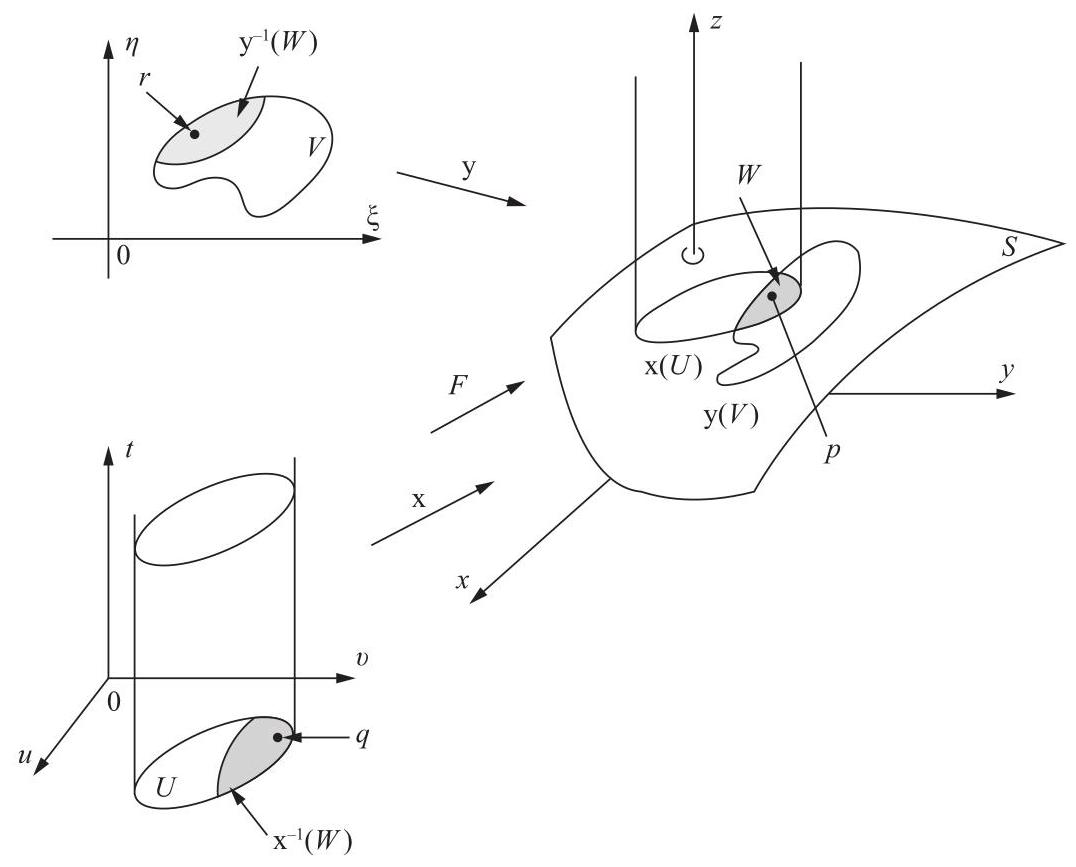
\includegraphics[max width=0.9\textwidth]{images/bo_d4b9jf3ef24c73e0334g_84_243_201_1076_867_0.jpg}
\end{center}
\hspace*{3em} 

图 2-14

其中函数 \(\xi\) 和 \(\eta\) 也具有所有阶的偏导数.因为

\[
\frac{\partial \left( {u,v}\right) }{\partial \left( {\xi ,\eta }\right) } \cdot  \frac{\partial \left( {\xi ,\eta }\right) }{\partial \left( {u,v}\right) } = 1,
\]

这意味着 \(h\) 和 \({h}^{-1}\) 的雅可比行列式处处非零.

命题 1 的证明. \(h = {\mathbf{x}}^{-1} \circ  \mathbf{y}\) 是一个同胚，因为它是由同胚组成的(参见第 2 章附录，命题 3).不能通过类似的论证得出 \(h\) 是可微的，因为 \({\mathbf{x}}^{-1}\) 定义在 \(S\) 的一个开子集上，而我们还不知道 \(S\) 上的可微函数是什么意思.

我们按以下方式进行.令 \(r \in  {\mathbf{y}}^{-1}\left( W\right)\) 并设 \(q = h\left( r\right)\) .由于 \(\mathbf{x}\left( {u,v}\right)  = \left( {x\left( {u,v}\right) ,y\left( {u,v}\right) ,z\left( {u,v}\right) }\right)\) 是一个参数化，我们可以假设，如果需要，通过重命名坐标轴，使得

\[
\frac{\partial \left( {x,y}\right) }{\partial \left( {u,v}\right) }\left( q\right)  \neq  0.
\]

我们将 \(\mathbf{x}\) 扩展为一个映射 \(F : U \times  R \rightarrow  {R}^{3}\) ，定义为

\[
F\left( {u,v,t}\right)  = \left( {x\left( {u,v}\right) ,y\left( {u,v}\right) ,z\left( {u,v}\right)  + t}\right) ,\;\left( {u,v}\right)  \in  U,t \in  R.
\]

几何上， \(F\) 将 \(U\) 上的一个垂直圆柱体 \(C\) 映射到 \(\mathbf{x}\left( U\right)\) 上的一个“垂直圆柱体”，方法是将 \(C\) 中高度为 \(t\) 的每个截面映射到曲面 \(\mathbf{x}\left( {u,v}\right)  + \; t{e}_{3}\) ，其中 \({e}_{3}\) 是 \(z\) 轴的单位向量(图 2-14).

显然， \(F\) 是可微的，并且限制 \(F \mid  U \times  \{ 0\}  = \mathbf{x}\) .计算微分 \(d{F}_{q}\) 的行列式，我们得到

\[
\left| \begin{array}{lll} \frac{\partial x}{\partial u} & \frac{\partial x}{\partial v} & 0 \\  \frac{\partial y}{\partial u} & \frac{\partial y}{\partial v} & 0 \\  \frac{\partial z}{\partial u} & \frac{\partial z}{\partial v} & 1 \end{array}\right|  = \frac{\partial \left( {x,y}\right) }{\partial \left( {u,v}\right) }\left( q\right)  \neq  0.
\]

因此，可以应用反函数定理，该定理保证在 \({R}^{3}\) 中存在 \(\mathbf{x}\left( q\right)\) 的一个邻域 \(M\) ，使得 \({F}^{-1}\) 在 \(M\) 中存在且可微.

由于 \(\mathbf{y}\) 的连续性，存在 \(V\) 中 \(r\) 的一个邻域 \(N\) ，使得 \(\mathbf{y}\left( N\right)  \subset  M\) (附录第 2 章，命题 2).注意，限制在 \(N\) 上， \(h\left| {N = {F}^{-1} \circ  \mathbf{y}}\right| N\) 是可微映射的复合.因此，我们可以应用映射的链式法则(附录第 2 章，命题 8)，并得出 \(h\) 在 \(r\) 处可微.由于 \(r\) 是任意的， \(h\) 在 \({\mathbf{y}}^{-1}\left( W\right)\) 上是可微的.

完全相同的论证可以用来证明映射 \({h}^{-1}\) 是可微的，因此 \(h\) 是一个微分同胚.Q.E.D.

现在我们将给出正则曲面上可微函数的明确定义.

定义 1. 令 \(\mathrm{f} : \mathrm{V} \subset  S \rightarrow  \mathbb{R}\) 为正则曲面 \(S\) 的一个开子集 \(\mathrm{V}\) 中定义的函数.则称 \(\mathrm{f}\) 在 \(\mathrm{p} \in  \mathrm{V}\) 处可微，如果存在一个参数化 \(\mathbf{x} : \mathrm{U} \subset  {\mathbb{R}}^{2} \rightarrow  S\) ，使得 \(\mathrm{p} \in  \mathbf{x}\left( \mathrm{U}\right)  \subset  \mathrm{V}\) ，则复合映射 \(\mathrm{f} \circ  \mathbf{x} : \mathrm{U} \subset  {\mathbb{R}}^{2} \rightarrow  \mathbb{R}\) 在 \({\mathbf{x}}^{-1}\left( \mathrm{p}\right)\) 处可微.如果 \(\mathrm{f}\) 在 \(\mathrm{V}\) 的所有点处都可微，则称 \(\mathrm{f}\) 在 \(\mathrm{V}\) 中可微.

由上一个命题直接得出，给定的定义不依赖于参数化 \(\mathbf{x}\) 的选择.事实上，如果 \(\mathbf{y} : V \subset \; {R}^{2} \rightarrow  S\) 是另一个参数化，且 \(p \in  \mathbf{y}\left( V\right)\) ，以及 \(h = {\mathbf{x}}^{-1} \circ  \mathbf{y}\) ，那么 \(f \circ  \mathbf{y} = f \circ  \mathbf{x} \circ  h\) 也是可微的，因此断言的独立性成立.

注1.我们经常会滥用符号，用同一个符号 \(f\left( {u,v}\right)\) 来表示 \(f\) 和 \(f \circ  \mathbf{x}\) ，并说 \(f\left( {u,v}\right)\) 是 \(f\) 在坐标系 \(\mathbf{x}\) 中的表达式.这等同于将 \(\mathbf{x}\left( U\right)\) 与 \(U\) 视为同一事物，并可以不加区分地将 \(\left( {u,v}\right)\) 看作是 \(U\) 中的一个点，也是 \(\mathbf{x}\left( U\right)\) 中的一个点，其坐标为 \(\left( {u,v}\right)\) .从现在起，此类语言上的滥用将不再另行说明.

例1.设 \(S\) 是一个正则曲面， \(V \subset  {R}^{3}\) 是一个开集，使得 \(S \subset  V\) .设 \(f : V \subset  {R}^{3} \rightarrow  R\) 是一个可微函数.那么 \(f\) 在 \(S\) 上的限制是在 \(S\) 上的一个可微函数.事实上，对于任何 \(p \in  S\) 和在 \(p\) 中的任何参数化 \(\mathbf{x} : U \subset  {R}^{2} \rightarrow  S\) ，函数 \(f \circ  \mathbf{x} : U \rightarrow  R\) 都是可微的.特别地，以下函数是可微的:

1. 相对于单位向量 \(v \in  {R}^{3},h : S \rightarrow  R\) 的高度函数，由 \(h\left( p\right)  = p \cdot  v,p \in  S\) 给出，其中点表示 \({R}^{3}.h\left( p\right)\) 中的通常内积，是 \(p \in  S\) 相对于法向量为 \(v\) 且通过 \({R}^{3}\) 的原点的平面高度(图 2-15).

\begin{center}
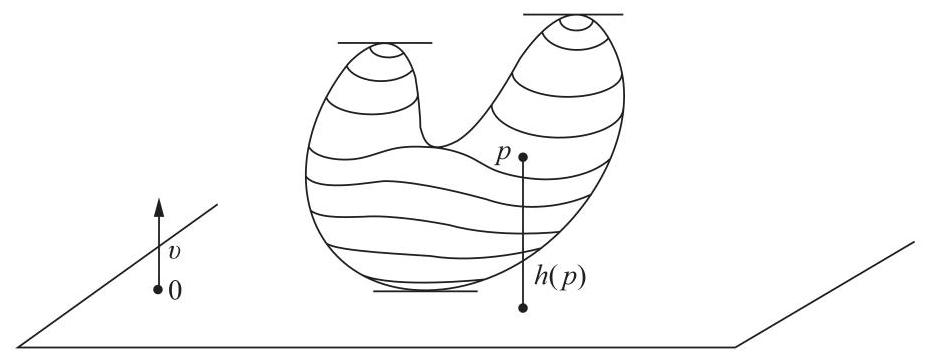
\includegraphics[max width=0.8\textwidth]{images/bo_d4b9jf3ef24c73e0334g_86_318_841_930_360_0.jpg}
\end{center}
\hspace*{3em} 

图 2-15

2. 与固定点 \({p}_{0} \in  {R}^{3},\;f\left( p\right)  = \; {\left| p - {p}_{0}\right| }^{2},p \in  S\) 的距离的平方.之所以需要取平方，是因为距离 \(\left| {p - {p}_{0}}\right|\) 在 \(p = {p}_{0}\) 处不可微.

注2.命题1的证明实质上利用了参数化逆是连续的事实.由于我们需要命题1来定义曲面上的可微函数(一个至关重要的概念)，因此在正则曲面的定义中不能省略这个条件(参见第 2-2 节的注1).

可微性的定义可以很容易地推广到曲面之间的映射.一个连续映射 \(\varphi  : {V}_{1} \subset  {S}_{1} \rightarrow  {S}_{2}\) ，从正则曲面 \({S}_{1}\) 的一个开集 \({V}_{1}\) 到正则曲面 \({S}_{2}\) ，如果在 \(p \in  {V}_{1}\) 处给定参数化

\[
{\mathbf{x}}_{1} : {U}_{1} \subset  {R}^{2} \rightarrow  {S}_{1}\;{\mathbf{x}}_{2} : {U}_{2} \subset  {R}^{2} \rightarrow  {S}_{2},
\]

其中 \(p \in  {\mathbf{x}}_{1}\left( U\right)\) 和 \(\varphi \left( {{\mathbf{x}}_{1}\left( {U}_{1}\right) }\right)  \subset  {\mathbf{x}}_{2}\left( {U}_{2}\right)\) ，映射

\[
{\mathbf{x}}_{2}^{-1} \circ  \varphi  \circ  {\mathbf{x}}_{1} : {U}_{1} \rightarrow  {U}_{2}
\]

在 \(q = {\mathbf{x}}_{1}^{-1}\left( p\right)\) 处可微(图 2-16).

\begin{center}
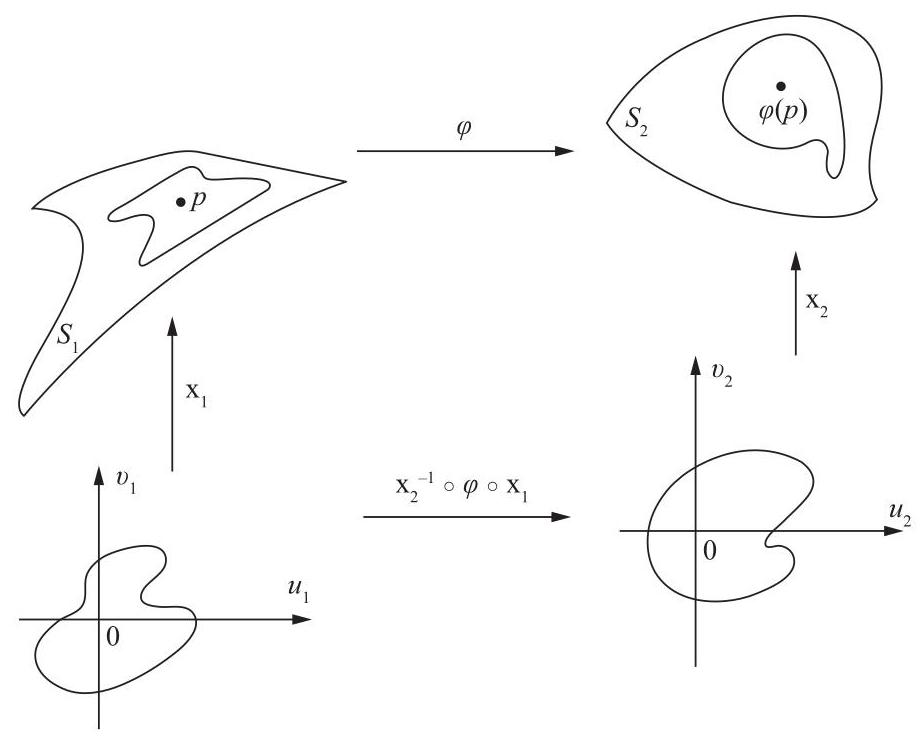
\includegraphics[max width=0.8\textwidth]{images/bo_d4b9jf3ef24c73e0334g_87_300_189_923_740_0.jpg}
\end{center}
\hspace*{3em} 

图 2-16

换句话说，如果 \(\varphi\) 在局部坐标下表示为 \(\varphi \left( {{u}_{1},{v}_{1}}\right)  = \left( {{\varphi }_{1}\left( {{u}_{1},{v}_{1}}\right) ,{\varphi }_{2}\left( {{u}_{1},{v}_{1}}\right) }\right)\) 时，函数 \({\varphi }_{1}\) 和 \({\varphi }_{2}\) 具有所有阶的连续偏导数，则 \(\varphi\) 是可微的.

此定义不依赖于参数选择的证明留作练习.

我们应该提到，与可微性相关的自然等价概念是微分同胚的概念.两个正则曲面 \({S}_{1}\) 和 \({S}_{2}\) 是微分同胚的，如果存在一个可微映射 \(\varphi  : {S}_{1} \rightarrow  {S}_{2}\) 及其可微逆映射 \({\varphi }^{-1} : {S}_{2} \rightarrow  {S}_{1}\) .这样的 \(\varphi\) 被称为从 \({S}_{1}\) 到 \({S}_{2}\) 的微分同胚.微分同胚的概念在正则曲面研究中所起的作用，与同构概念在向量空间研究中所起的作用，或与全等概念在欧几里得几何中所起的作用相同.换句话说，从可微性的角度来看，两个微分同胚的曲面是无法区分的.

例 2. 如果 \(\mathbf{x} : U \subset  {R}^{2} \rightarrow  S\) 是一个参数化， \({\mathbf{x}}^{-1} : \mathbf{x}\left( U\right)  \rightarrow  {R}^{2}\) 是可微的.事实上，对于任何 \(p \in  \mathbf{x}\left( U\right)\) 和 \(p\) 中的任何参数化 \(\mathbf{y} : V \subset \; {R}^{2} \rightarrow  S\) ，我们有 \({\mathbf{x}}^{-1} \circ  \mathbf{y} : {\mathbf{y}}^{-1}\left( W\right)  \rightarrow  {\mathbf{x}}^{-1}\left( W\right)\) ，其中

\[
W = \mathbf{x}\left( U\right)  \cap  \mathbf{y}\left( V\right)
\]

是可微的.这表明 \(U\) 和 \(\mathbf{x}\left( U\right)\) 是微分同胚的(即，每个正则曲面在局部上都与平面微分同胚)，并证明了注 1 中所做的识别.

例 3. 令 \({S}_{1}\) 和 \({S}_{2}\) 为正则曲面.假设 \({S}_{1} \subset  V \subset  {R}^{3}\) ，其中 \(V\) 是 \({R}^{3}\) 的一个开集，并且 \(\varphi  : V \rightarrow  {R}^{3}\) 是一个可微映射，使得 \(\varphi \left( {S}_{1}\right)  \subset  {S}_{2}\) .那么限制 \(\varphi  \mid  {S}_{1} : {S}_{1} \rightarrow  {S}_{2}\) 是一个可微映射.事实上，给定 \(p \in  {S}_{1}\) 和参数化 \({\mathbf{x}}_{1} : {U}_{1} \rightarrow  {S}_{1},{\mathbf{x}}_{2} : {U}_{2} \rightarrow  {S}_{2}\) ，其中 \(p \in  {\mathbf{x}}_{1}\left( {U}_{1}\right)\) 和 \(\varphi \left( {{\mathbf{x}}_{1}\left( {U}_{1}\right) }\right)  \subset  {\mathbf{x}}_{2}\left( {U}_{2}\right)\) ，我们有映射

\[
{\mathbf{x}}_{2}^{-1} \circ  \varphi  \circ  {\mathbf{x}}_{1} : {U}_{1} \rightarrow  {U}_{2}
\]

是可微的.以下是这个一般例子的特例:

1. 设 \(S\) 关于 \({xy}\) 平面对称；也就是说，如果 \(\left( {x,y,z}\right)  \in  S\) ，那么也 \(\left( {x,y, - z}\right)  \in  S\) .那么映射 \(\sigma  : S \rightarrow  S\) ，它将 \(p \in  S\) 映射到其对称点，是可微的，因为它是 \(\sigma  : {R}^{3} \rightarrow  {R}^{3},\sigma \left( {x,y,z}\right)  = \left( {x,y, - z}\right)\) 在 \(S\) 上的限制.当然，这可以推广到关于任意 \({R}^{3}\) 平面对称的曲面.

2. 设 \({R}_{z,\theta } : {R}^{3} \rightarrow  {R}^{3}\) 是绕 \(z\) 轴旋转 \(\theta\) 角的旋转，设 \(S \subset  {R}^{3}\) 是不变于此旋转的正則曲面；即，如果 \(p \in  S\) ，则 \({R}_{z,\theta }\left( p\right)  \in  S\) .那么限制 \({R}_{z,\theta } : S \rightarrow  S\) 是一个可微映射.

3. 设 \(\varphi  : {R}^{3} \rightarrow  {R}^{3}\) 由 \(\varphi \left( {x,y,z}\right)  = \left( {{xa},{yb},{zc}}\right)\) 给出，其中 \(a,b\) 和 \(c\) 是非零实数. \(\varphi\) 显然是可微的，并且限制 \(\varphi  \mid  {S}^{2}\) 是从球面到

\[
{S}^{2} = \left\{  {\left( {x,y,z}\right)  \in  {R}^{3};{x}^{2} + {y}^{2} + {z}^{2} = 1}\right\}
\]

到椭球面的一个可微映射

\[
\left\{  {\left( {x,y,z}\right)  \in  {R}^{3};\frac{{x}^{2}}{{a}^{2}} + \frac{{y}^{2}}{{b}^{2}} + \frac{{z}^{2}}{{c}^{2}} = 1}\right\}
\]

(参见附录第 2 章的示例 6).

注 3. 命题 1 表明(参见示例 2)，参数化 \(\mathbf{x} : U \subset  {R}^{2} \rightarrow  S\) 是 \(U\) 到 \(\mathbf{x}\left( U\right)\) 的一个微分同胚.实际上，我们现在可以将正則曲面刻画为那些局部上与 \({R}^{2}\) 微分同胚的子集 \(S \subset  {R}^{3}\) ；也就是说，对于每个点 \(p \in  S\) ，存在 \(S\) 中 \(p\) 的一个邻域 \(V\) ，一个开集 \(U \subset  {R}^{2}\) ，以及一个映射 \(\mathbf{x} : U \rightarrow  V\) ，它是一个微分同胚.这个优美的刻画可以作为曲面处理的起点(参见练习 13).

此时，我们可以回到曲线的理论，并从本章的角度来处理它们，即作为 \({R}^{3}\) 的子集.我们将只提及一些基本要点，并将细节留给读者.

符号 \(I\) 将表示直线 \(R\) 上的一个开区间. \({R}^{3}\) 中的正則曲线是一个子集 \(C \subset  {R}^{3}\) ，具有以下性质:对于每个点 \(p \in  C\) ，存在 \({R}^{3}\) 中 \(p\) 的一个邻域 \(V\) 和一个可微同胚 \(\alpha  : I \subset  R \rightarrow  V \cap  C\) ，使得对于每个 \(t \in  I\) ，微分 \(d{\alpha }_{t}\) 是一对一的(图 2-17).

\begin{center}
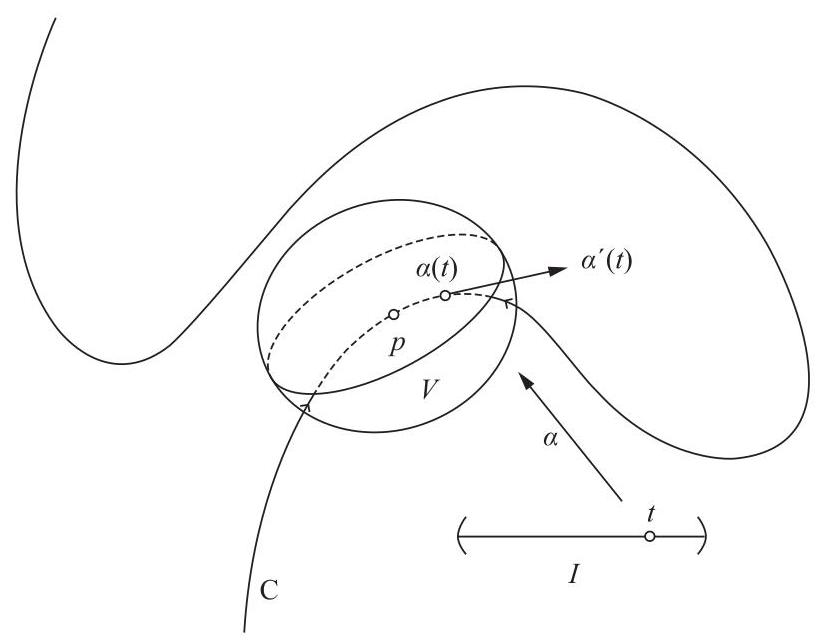
\includegraphics[max width=0.7\textwidth]{images/bo_d4b9jf3ef24c73e0334g_89_353_188_823_643_0.jpg}
\end{center}
\hspace*{3em} 

图 2-17. 正則曲线.

可以证明(练习 15)，参数变换由一个微分同胚给出(与曲面一样).从这个基本结果出发，可以决定通过参数变换获得的某个性质是否独立于该参数变换.这样的性质将是集合 \(C\) 的局部性质.

例如，结果表明，在第 1 章中定义的弧长与所选的参数化无关(练习 15)，因此是集合 \(C\) 的一个性质.由于总有可能通过弧长局部参数化一条正则曲线 \(C\) ，因此通过这种参数化确定的性质(曲率、挠率等)是 \(C\) 的局部性质.这表明第 1 章中发展的曲线局部理论对于正则曲线是有效的.

有时，曲面是通过以指定的方式移动某条正则曲线来定义的.这在以下示例中会出现.

例 4(旋转曲面).设 \(S \subset  {R}^{3}\) 是通过围绕平面上不与曲线相交的轴旋转一条正则连通平面曲线 \(C\) 而得到的集合；我们将取 \({xz}\) 平面作为曲线所在的平面，并将 \(z\) 轴作为旋转轴.设

\[
x = f\left( v\right) ,\;z = g\left( v\right) ,\;a < v < b,\;f\left( v\right)  > 0,
\]

是 \(C\) 的一个参数化，并用 \(u\) 表示绕 \(z\) 轴的旋转角度.因此，我们得到一个映射

\[
\mathbf{x}\left( {u,v}\right)  = \left( {f\left( v\right) \cos u,f\left( v\right) \sin u,g\left( v\right) }\right)
\]

从开集 \(U = \left\{  {\left( {u,v}\right)  \in  {R}^{2};0 < u < {2\pi },a < v < b}\right\}\) 到 \(S\) (图 2-18).

\begin{center}
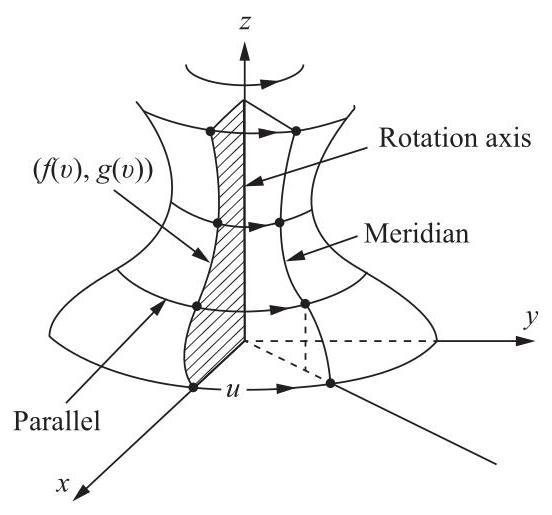
\includegraphics[max width=0.5\textwidth]{images/bo_d4b9jf3ef24c73e0334g_90_196_200_552_515_0.jpg}
\end{center}
\hspace*{3em} 

图 2-18.旋转曲面.

我们很快就会看到 \(\mathbf{x}\) 满足正则曲面定义中的参数化条件.由于 \(S\) 可以被类似的参数化完全覆盖，因此 \(S\) 是一个正则曲面，称为旋转曲面.曲线 \(C\) 称为 \(S\) 的生成曲线， \(z\) 轴是 \(S\) 的旋转轴.由 \(C\) 的点描述的圆称为 \(S\) 的纬线， \(C\) 在 \(S\) 上的各种位置称为 \(S\) 的经线.

为了证明 \(\mathbf{x}\) 是 \(S\) 的参数化，我们必须检查定义 1，第 2-2 节的条件 1、2 和 3.条件 1 和 3 是直接的，我们留给读者.为了证明 \(\mathbf{x}\) 是一个同胚，我们首先证明 \(\mathbf{x}\) 是一一对应的.事实上，由于 \(\left( {f\left( v\right) ,g\left( v\right) }\right)\) 是 \(C\) 的参数化，给定 \(z\) 和 \({x}^{2} + {y}^{2} = {\left( f\left( v\right) \right) }^{2}\) ，我们可以唯一地确定 \(v\) .因此， \(\mathbf{x}\) 是一一对应的.

我们注意到，同样因为 \(\left( {f\left( v\right) ,g\left( v\right) }\right)\) 是 \(C,v\) 的参数化， \(C,v\) 是 \(z\) 和 \(\sqrt{{x}^{2} + {y}^{2}}\) 的连续函数，因此是 \(\left( {x,y,z}\right)\) 的连续函数.

为了证明 \({\mathbf{x}}^{-1}\) 是连续的，剩下要证明的是 \(u\) 是 \(\left( {x,y,z}\right)\) 的连续函数.为了看到这一点，我们首先观察到，如果 \(u \neq  \pi\) ，我们得到，因为 \(f\left( v\right)  \neq  0\) ，

\[
\tan \frac{u}{2} = \frac{\sin \frac{u}{2}}{\cos \frac{u}{2}} = \frac{2\sin \frac{u}{2}\cos \frac{u}{2}}{2{\cos }^{2}\frac{u}{2}} = \frac{\sin u}{1 + \cos u}
\]

\[
= \frac{\frac{y}{f\left( v\right) }}{1 + \frac{x}{f\left( v\right) }} = \frac{y}{x + \sqrt{{x}^{2} + {y}^{2}}};
\]

因此，

\[
u = 2{\tan }^{-1}\frac{y}{x + \sqrt{{x}^{2} + {y}^{2}}}.
\]

因此，如果 \(u \neq  \pi ,u\) 是 \(\left( {x,y,z}\right)\) 的连续函数.同样，如果 \(u\) 在 \(\pi\) 的一个小的区间内，我们得到

\[
u = 2{\operatorname{cotan}}^{-1}\frac{y}{-x + \sqrt{{x}^{2} + {y}^{2}}}.
\]

因此， \(u\) 是 \(\left( {x,y,z}\right)\) 的连续函数.这表明 \({\mathbf{x}}^{-1}\) 是连续的，并完成了验证.

备注 4. 我们的旋转曲面定义存在一个小问题.如果 \(C \subset  {R}^{2}\) 是一条闭合的正则平面曲线，且关于 \({R}^{3}\) 的轴 \(r\) 对称，那么通过将 \(C\) 绕 \(r\) 旋转，我们可以得到一个可以证明是正则的曲面，并且也应该称为旋转曲面(当 \(C\) 是圆且 \(r\) 包含 \(C\) 的一个直径时，该曲面是球面).为了符合我们的定义，我们需要排除它的两个点，即 \(r\) 与 \(C\) 相交的点.出于技术原因，我们希望保持之前的术语，并将后者称为扩展旋转曲面.

现在应该对我们曲面的定义做一个最后的评论.我们选择将一个(正则)曲面定义为 \({R}^{3}\) 的一个子集.如果我们想考虑曲面的全局和局部性质，这是正确的设定.然而，读者可能想知道，为什么我们没有像曲线那样简单地将曲面定义为参数化曲面.这可以做到，事实上，微分几何的某些经典文献就是这样呈现的.只要只考虑局部性质，就不会造成严重的损害.然而，像定向(将在第2-6节和3-1节中讨论)这样的基本全局概念，在这种方法下必须被省略或处理不当.

无论如何，参数化曲面的概念有时是有用的，并且应该包含在这里.

定义2. 参数化曲面 \(\mathbf{x} : \mathrm{U} \subset  {\mathbb{R}}^{2} \rightarrow  {\mathbb{R}}^{3}\) 是一个从开集 \(\mathrm{U} \subset  {\mathbb{R}}^{2}\) 到 \({\mathbb{R}}^{3}\) 的可微映射 \(\mathbf{x}\) .集合 \(\mathbf{x}\left( \mathrm{U}\right)  \subset  {\mathbb{R}}^{3}\) 称为 \(\mathbf{x}.\mathbf{x}\) 的轨迹，如果微分 \({\mathrm{{dx}}}_{\mathrm{q}} : {\mathbb{R}}^{2} \rightarrow  {\mathbb{R}}^{3}\) 对所有 \(\mathrm{q} \in  \mathrm{U}\) 都是一对一的(即，向量 \(\partial \mathbf{x}/\partial u,\partial \mathbf{x}/\partial v\) 对所有 \(\mathrm{q} \in  \mathrm{U}\) 线性无关).点 \(\mathrm{p} \in  \mathrm{U}\) ，其中 \(d{\mathbf{x}}_{p}\) 不是一对一的，称为 \(\mathbf{x}\) 的奇异点.

请注意，即使是正则的参数化曲面，其轨迹也可能存在自交点.

例5. 令 \(\alpha  : I \rightarrow  {R}^{3}\) 为一个非平面的正则参数化曲线.定义

\[
\mathbf{x}\left( {t,v}\right)  = \alpha \left( t\right)  + v{\alpha }^{\prime }\left( t\right) ,\;\left( {t,v}\right)  \in  I \times  R.
\]

\(\mathbf{x}\) 是一个参数化曲面，称为 \(\alpha\) 的切面(图2-19).

\begin{center}
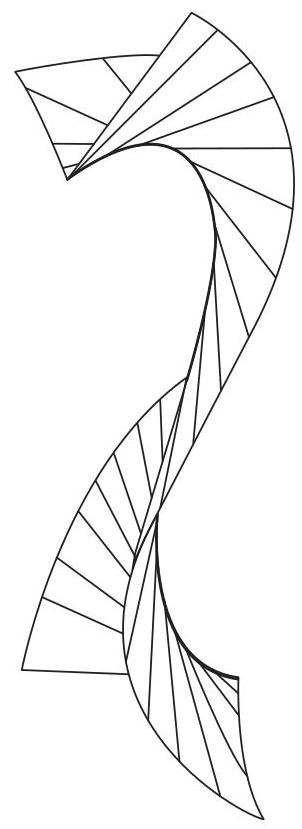
\includegraphics[max width=0.2\textwidth]{images/bo_d4b9jf3ef24c73e0334g_92_633_461_302_829_0.jpg}
\end{center}
\hspace*{3em} 

图2-19. 切面.

现在假设 \(\alpha\) 的曲率 \(k\left( t\right) ,t \in  I\) 对所有 \(t \in  I\) 都非零，并将 \(\mathbf{x}\) 的定义域限制在 \(U = \{ \left( {t,v}\right)  \in  I \times  R;v \neq  0\}\) 上.那么

\[
\frac{\partial \mathbf{x}}{\partial t} = {\alpha }^{\prime }\left( t\right)  + v{\alpha }^{\prime \prime }\left( t\right) ,\;\frac{\partial \mathbf{x}}{\partial v} = {\alpha }^{\prime }\left( t\right)
\]

和

\[
\frac{\partial \mathbf{x}}{\partial t} \land  \frac{\partial \mathbf{x}}{\partial v} = v{\alpha }^{\prime \prime }\left( t\right)  \land  {\alpha }^{\prime }\left( t\right)  \neq  0,\;\left( {t,v}\right)  \in  U,
\]

因为对于所有 \(t\) ，曲率(参见第1-5节的练习12)

\[
k\left( t\right)  = \frac{\left| {\alpha }^{\prime \prime }\left( t\right)  \land  {\alpha }^{\prime }\left( t\right) \right| }{{\left| {\alpha }^{\prime }\left( t\right) \right| }^{3}}
\]

非零.因此，限制 \(\mathbf{x} : U \rightarrow  {R}^{3}\) 是一个正则参数化曲面，其轨迹由两个连通部分组成，它们的公共边界是集合 \(\alpha \left( I\right)\) .

下面的命题表明，我们可以将微分几何的局部概念和性质推广到正则参数化曲面.

命题 2. 设 \(x : \mathrm{U} \subset  {\mathbb{R}}^{2} \rightarrow  {\mathbb{R}}^{3}\) 为一个正则参数化曲面，设 \(\mathrm{q} \in  \mathrm{U}\) .则存在 \({\mathbb{R}}^{2}\) 中的 \(\mathrm{q}\) 的一个邻域 \(\mathrm{V}\) ，使得 \(\mathbf{x}\left( \mathrm{V}\right)  \subset  {\mathbb{R}}^{3}\) 是一个正则曲面.

证明. 这仍然是反函数定理的一个推论.写出

\[
\mathbf{x}\left( {u,v}\right)  = \left( {x\left( {u,v}\right) ,y\left( {u,v}\right) ,z\left( {u,v}\right) }\right) .
\]

根据正则性，我们可以假设 \(\left( {\partial \left( {x,y}\right) /\partial \left( {u,v}\right) }\right) \left( q\right)  \neq  0\) .定义一个映射 \(F : U \times  R \rightarrow  {R}^{3}\) 为

\[
F\left( {u,v,t}\right)  = \left( {x\left( {u,v}\right) ,y\left( {u,v}\right) ,z\left( {u,v}\right)  + t}\right) ,\;\left( {u,v}\right)  \in  U,t \in  R.
\]

然后

\[
\det \left( {d{F}_{q}}\right)  = \frac{\partial \left( {x,y}\right) }{\partial \left( {u,v}\right) }\left( q\right)  \neq  0.
\]

根据反函数定理，存在 \({W}_{1}\) 的邻域 \(q\) 和 \({W}_{2}\) 的邻域 \(F\left( q\right)\) ，使得 \(F : {W}_{1} \rightarrow  {W}_{2}\) 是一个微分同胚.令 \(V = {W}_{1} \cap  U\) ，并观察到限制 \(F\left| {V = \mathbf{x}}\right| V\) .因此， \(\mathbf{x}\left( V\right)\) 与 \(V\) 微分同胚，从而是一个正则曲面.证毕.

\exerciseline

*1. 令 \({S}^{2} = \left\{  {\left( {x,y,z}\right)  \in  {R}^{3};{x}^{2} + {y}^{2} + {z}^{2} = 1}\right\}\) 为单位球面，令 \(A : {S}^{2} \rightarrow  {S}^{2}\) 为(对径)映射 \(A\left( {x,y,z}\right)  = \left( {-x, - y, - z}\right)\) .证明 \(A\) 是一个微分同胚.

2. 令 \(S \subset  {R}^{3}\) 为一个正则曲面，令 \(\pi  : S \rightarrow  {R}^{2}\) 为将每个 \(p \in  S\) 映射到其在 \({R}^{2} = \left\{  {\left( {x,y,z}\right)  \in  {R}^{3}}\right.\) 上的正交投影的映射； \(z = 0\}\) . \(\pi\) 是可微的吗？

3. 证明抛物面 \(z = {x}^{2} + {y}^{2}\) 与平面微分同胚.

4. 构建椭球体

\[
\frac{{x}^{2}}{{a}^{2}} + \frac{{y}^{2}}{{b}^{2}} + \frac{{z}^{2}}{{c}^{2}} = 1
\]

与球面 \({x}^{2} + {y}^{2} + {z}^{2} = 1\) 之间的微分同胚.

*5. 令 \(S \subset  {R}^{3}\) 为一个正则曲面，令 \(d : S \rightarrow  R\) 由 \(d\left( p\right)  = \; \left| {p - {p}_{0}}\right|\) 给出，其中 \(p \in  S,{p}_{0} \neq  {R}^{3},{p}_{0} \notin  S\) ；也就是说， \(d\) 是 \(p\) 到固定点 \({p}_{0}\) (不在 \(S\) 中)的距离.证明 \(d\) 是可微的.



\(\dagger\) 那些省略了本节证明的人也应省略练习 13-16.



6. 证明曲面之间可微映射的定义不依赖于所选的参数化.

7. 证明“ \({S}_{1}\) 与 \({S}_{2}\) 微分同胚”的关系是正则曲面集合上的一个等价关系.

*8. 令 \({S}^{2} = \left\{  {\left( {x,y,z}\right)  \in  {R}^{3};{x}^{2} + {y}^{2} + {z}^{2} = 1}\right\}\) 和 \(H = \left\{  {\left( {x,y,z}\right)  \in  {R}^{3}}\right.\) ； \({x}^{2} + {\mathbf{y}}^{2} - {z}^{2} = 1\}\) .分别用 \(N = \left( {0,0,1}\right)\) 和 \(S = \left( {0,0, - 1}\right)\) 表示 \({S}^{2}\) 的北极和南极，令 \(F : {S}^{2} - \{ N\}  \cup  \{ S\}  \rightarrow  H\) 定义如下:对于每个 \(p \in  {S}^{2} - \{ N\}  \cup  \{ S\}\) ，令从 \(p\) 到 \(z\) 轴的垂线与 \({0z}\) 相交于 \(q\) .考虑从 \(q\) 开始并经过 \(p\) 的半直线 \(l\) .则 \(F\left( p\right)  = l \cap  H\) (图 2-20).证明 \(F\) 是可微的.

\begin{center}
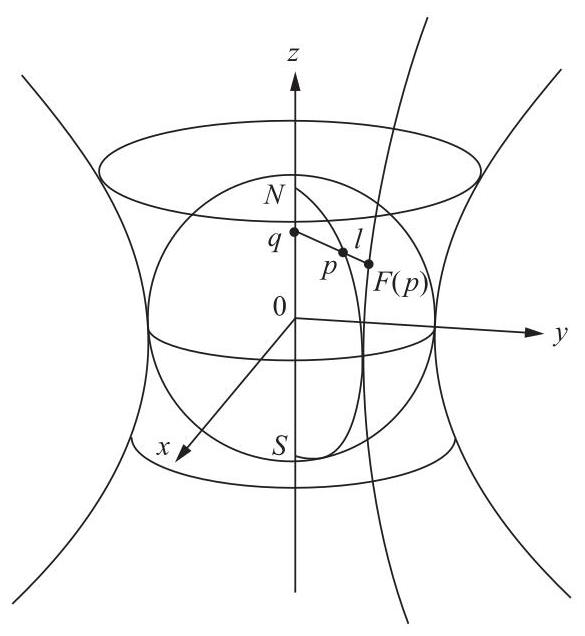
\includegraphics[max width=0.5\textwidth]{images/bo_d4b9jf3ef24c73e0334g_94_199_756_585_636_0.jpg}
\end{center}
\hspace*{3em} 

图 2-20

9. a. 定义正则曲线上的可微函数概念.为了使定义有意义，需要证明什么？现在不要证明.如果你没有省略本节的证明，将在练习 15 中要求你这样做.

b. 证明映射 \(E : R \rightarrow  {S}^{1} = \left\{  {\left( {x,y}\right)  \in  {R}^{2};{x}^{2} + {y}^{2} = 1}\right\}\) 由下式给出

\[
E\left( t\right)  = \left( {\cos t,\sin t}\right) ,\;t \in  R,
\]

是可微的(几何上， \(E\) 将 \(R\) “绕” \({S}^{1}\) “缠绕”).

10. 令 \(C\) 为平面正则曲线，它位于平面直线 \(r\) 的一侧，并与 \(r\) 在点 \(p,q\) 相交(图 2-21). \(C\) 应满足什么条件才能确保 \(C\) 绕 \(r\) 的旋转生成一个扩展的(正则)旋转曲面？

\begin{center}
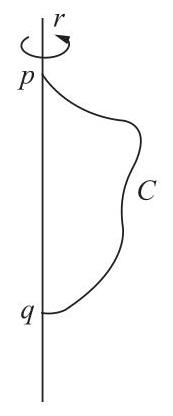
\includegraphics[max width=0.2\textwidth]{images/bo_d4b9jf3ef24c73e0334g_95_551_202_173_416_0.jpg}
\end{center}
\hspace*{3em} 

图 2-21

11. 证明旋转曲面 \(S\) 绕其轴的旋转是 \(S\) 的微分同胚.

12. 参数化曲面常用于描述除有限个点和有限条直线外均为正则曲面的集合 \(\sum\) .例如，令 \(C\) 为不通过原点 \(O = \left( {0,0,0}\right)\) 的正则参数化曲线 \(\alpha  : \left( {a,b}\right)  \rightarrow  {R}^{3}\) 的轨迹.令 \(\sum\) 为由通过移动点 \(p \in  C\) 和固定点 0 的直线 \(l\) 的位移生成的集合(以 0 为顶点的锥体；见图 2-22).

\begin{center}
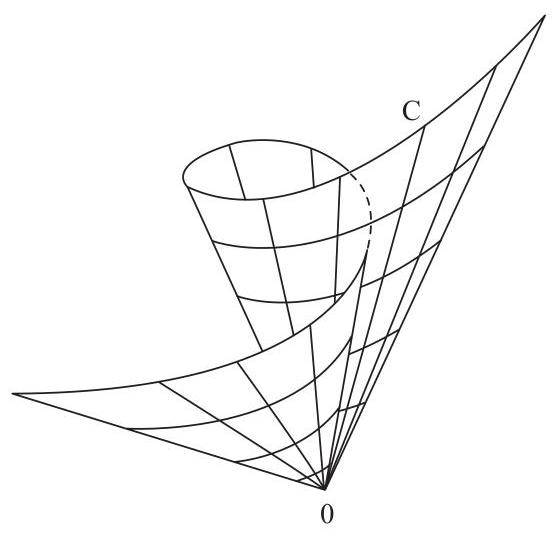
\includegraphics[max width=0.5\textwidth]{images/bo_d4b9jf3ef24c73e0334g_95_360_1157_560_538_0.jpg}
\end{center}
\hspace*{3em} 

图 2-22

a. 找到一个轨迹为 \(\sum\) 的参数化曲面 \(\mathbf{x}\) .

b. 找到 \(\mathbf{x}\) 不正则的点.

c. 从 \(\sum\) 中应移除什么，才能使剩余的集合成为正则曲面？

*13. 证明文本中给出的函数 \(f : V \subset  S \rightarrow  R\) 的可微性定义(定义 1)等价于以下定义:如果 \(f\) 是 \({R}^{3}\) 中包含 \(p\) 的开集上定义的某个可微函数的 \(V\) 上的限制，则 \(f\) 在 \(p \in  V\) 中是可微的.(如果我们从这个可微性定义开始，我们就可以将曲面定义为局部上与 \({R}^{2}\) 同胚的集合；见注 3.)

14. 令 \(A \subset  S\) 为正则曲面 \(S\) 的一个子集.证明 \(A\) 本身是一个正则曲面，当且仅当 \(A\) 在 \(S\) 中是开集；也就是说， \(A = U \cap  S\) ，其中 \(U\) 是 \({R}^{3}\) 中的一个开集.

15. 令 \(C\) 为一条正则曲线，令 \(\alpha  : I \subset  R \rightarrow  C,\beta  : J \subset  R \rightarrow  C\) 为 \(C\) 在 \(p \in  \alpha \left( I\right)  \cap  \beta \left( J\right)  = W\) 的邻域中的两个参数化.令

\[
h = {\alpha }^{-1} \circ  \beta  : {\beta }^{-l}\left( W\right)  \rightarrow  {\alpha }^{-l}\left( W\right)
\]

为参数变换.证明

a. \(h\) 是一个微分同胚.

b. \(C\) 在 \(W\) 中的弧长绝对值不依赖于选择哪个参数化来定义它，也就是说，

\[
\left| {{\int }_{{t}_{0}}^{t}\left| {{\alpha }^{\prime }\left( t\right) }\right| {dt}}\right|  = \left| {{\int }_{{\tau }_{0}}^{\tau }\left| {{\beta }^{\prime }\left( \tau \right) }\right| {d\tau }}\right| ,\;t = h\left( \tau \right) ,t \in  I,\tau  \in  J.
\]

*16. 令 \({R}^{2} = \left\{  {\left( {x,y,z}\right)  \in  {R}^{3};z =  - 1}\right\}\) 通过设置 \(\left( {x,y, - 1}\right)  = x + {iy} = \zeta  \in  \mathbb{C}\) 来识别为复平面 \(\mathbb{C}\) .令 \(P : \mathbb{C} \rightarrow  \mathbb{C}\) 为复多项式

\[
P\left( \zeta \right)  = {a}_{0}{\zeta }^{n} + {a}_{1}{\zeta }^{n - 1} + \cdots  + {a}_{n},\;{a}_{0} \neq  0,{a}_{i} \in  \mathbb{C},i = 0,\ldots ,n.
\]

记 \({\pi }_{N}\) 为 \({S}^{2} = \left\{  {\left( {x,y,z}\right)  \in  {R}^{3}}\right.\) 的球极投影； \(\left. {{x}^{2} + {y}^{2} + {z}^{2} = 1}\right\}\) 从北极 \(N = \left( {0,0,1}\right)\) 投影到 \({R}^{2}\) .证明映射 \(F : {S}^{2} \rightarrow  {S}^{2}\) 由

\[
F\left( p\right)  = {\pi }_{N}^{-1} \circ  P \circ  {\pi }_{N}\left( p\right) ,\;\text{ if }p \in  {S}^{2} - \{ N\} ,
\]

\[
F\left( N\right)  = N
\]

是可微的.

\section*{2-4. 切平面；映射的微分}

在本节中，我们将证明正则曲面 \(S\) 定义中的条件 3 保证对于每个 \(p \in  S\) ，通过 \(p\) 的 \(S\) 的参数化曲线的切向量集合构成一个平面.

我们称 \(S\) 在点 \(p \in  S\) 处的切向量为可微参数化曲线 \(\alpha  : \left( {-\epsilon ,\epsilon }\right)  \rightarrow  S\) 的切向量 \({\alpha }^{\prime }\left( 0\right)\) ，其中 \(\alpha \left( 0\right)  = p\) .

命题 1. 令 \(x : \mathrm{U} \subset  {\mathbb{R}}^{2} \rightarrow  S\) 为正则曲面 \(S\) 的一个参数化，令 \(\mathrm{q} \in  \mathrm{U}\) .二维向量子空间，

\[
{\mathrm{d}}_{{\mathbf{x}}_{\mathrm{q}}}\left( {\mathbb{R}}^{2}\right)  \subset  {\mathbb{R}}^{3},
\]

与 \(S\) 在 \(\mathbf{x}\left( \mathrm{q}\right)\) 处的切向量集合重合.

证明. 设 \(w\) 是 \(\mathbf{x}\left( q\right)\) 处的一个切向量，即设 \(w = {\alpha }^{\prime }\left( 0\right)\) ，其中 \(\alpha  : \left( {-\epsilon ,\epsilon }\right)  \rightarrow  \mathbf{x}\left( U\right)  \subset  S\) 是可微的且 \(\alpha \left( 0\right)  = \mathbf{x}\left( q\right)\) . 根据 2-3 节的例 2，曲线 \(\beta  = {\mathbf{x}}^{-1} \circ  \alpha  : \left( {-\epsilon ,\epsilon }\right)  \rightarrow  U\) 是可微的. 根据微分的定义(第 2 章附录，定义 1)，我们有 \(d{\mathbf{x}}_{q}\left( {{\beta }^{\prime }\left( 0\right) }\right)  = w\) . 因此， \(w \in  d{\mathbf{x}}_{q}\left( {R}^{2}\right)\) (图 2-23).

\begin{center}
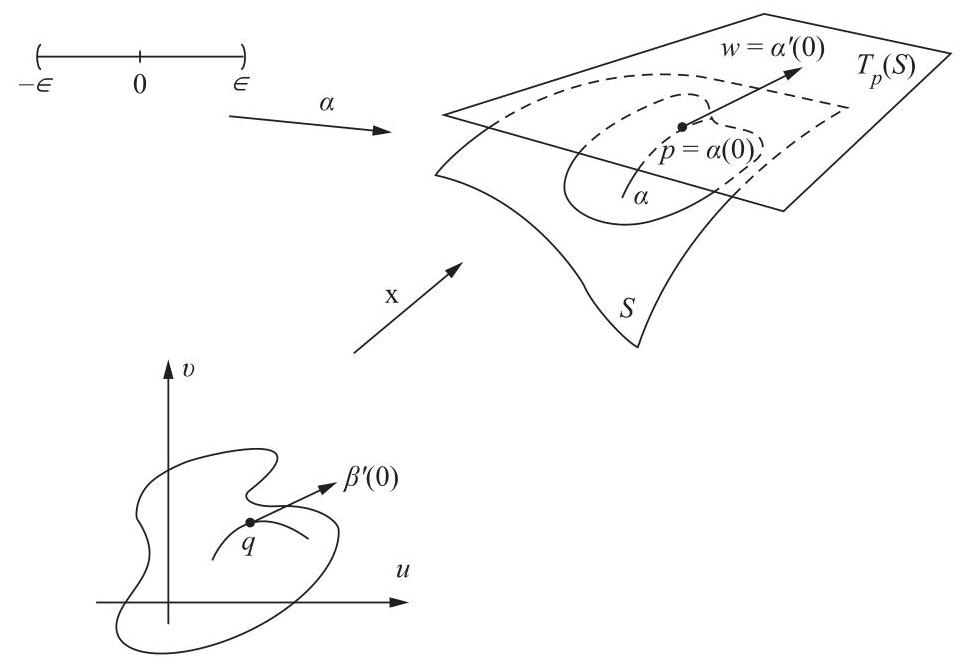
\includegraphics[max width=0.8\textwidth]{images/bo_d4b9jf3ef24c73e0334g_97_281_738_965_664_0.jpg}
\end{center}
\hspace*{3em} 

图 2-23

另一方面，设 \(w = d{\mathbf{x}}_{q}\left( v\right)\) ，其中 \(v \in  {R}^{2}\) . 显然 \(v\) 是由以下方式给出的曲线 \(\gamma  : \left( {-\epsilon ,\epsilon }\right)  \rightarrow  U\) 的速度向量:

\[
\gamma \left( t\right)  = {tv} + q,\;t \in  \left( {-\epsilon ,\epsilon }\right) .
\]

根据微分的定义， \(w = {\alpha }^{\prime }\left( 0\right)\) ，其中 \(\alpha  = \mathbf{x} \circ  \gamma\) . 这表明 \(w\) 是一个切向量.Q.E.D.

根据上述命题，平面 \(d{\mathbf{x}}_{q}\left( {R}^{2}\right)\) ，它通过 \(\mathbf{x}\left( q\right)  = p\) ，不依赖于参数化 \(\mathbf{x}\) . 这个平面将被称为 \(S\) 在 \(p\) 处的切平面，并记为 \({T}_{p}\left( S\right)\) . 参数化 \(\mathbf{x}\) 的选择确定了 \({T}_{p}\left( S\right)\) 的一个基 \(\{ \left( {\partial \mathbf{x}/\partial u}\right) \left( q\right) ,\left( {\partial \mathbf{x}/\partial v}\right) \left( q\right) \}\) ，称为与 \(\mathbf{x}\) 相关的基. 有时写成 \(\partial \mathbf{x}/\partial u = {\mathbf{x}}_{u}\) 和 \(\partial \mathbf{x}/\partial v = {\mathbf{x}}_{v}.\) 是方便的.

向量 \(w \in  {T}_{p}\left( S\right)\) 在与参数化 \(\mathbf{x}\) 相关的基中的坐标确定如下. \(w\) 是曲线 \({\alpha }^{\prime }\left( 0\right)\) 的速度向量 \(\alpha  = \mathbf{x} \circ  \beta\) ，其中 \(\beta  : \left( {-\epsilon ,\epsilon }\right)  \rightarrow  U\) 由 \(\beta \left( t\right)  = \left( {u\left( t\right) ,v\left( t\right) }\right)\) 给出，且 \(\beta \left( 0\right)  = q = {\mathbf{x}}^{-1}\left( p\right)\) . 因此，

\[
{\alpha }^{\prime }\left( 0\right)  = \frac{d}{dt}\left( {\mathbf{x} \circ  \beta }\right) \left( 0\right)  = \frac{d}{dt}\mathbf{x}\left( {u\left( t\right) ,v\left( t\right) }\right) \left( 0\right)
\]

\[
= {\mathbf{x}}_{u}\left( q\right) {u}^{\prime }\left( 0\right)  + {\mathbf{x}}_{v}\left( q\right) {v}^{\prime }\left( 0\right)  = w.
\]

因此，在基 \(\left\{  {{\mathbf{x}}_{u}\left( q\right) ,{\mathbf{x}}_{v}\left( q\right) }\right\}  ,w\) 中，坐标为 \(\left( {{u}^{\prime }\left( 0\right) ,{v}^{\prime }\left( 0\right) }\right)\) ，其中 \(\left( {u\left( t\right) ,v\left( t\right) }\right)\) 是参数化 \(\mathbf{x}\) 中曲线的速度向量在 \(t = 0\) 处为 \(w\) 的表达式.

有了切平面这个概念，我们就可以讨论曲面之间可微映射的微分了.设 \({S}_{1}\) 和 \({S}_{2}\) 是两个正则曲面，设 \(\varphi  : V \subset  {S}_{1} \rightarrow  {S}_{2}\) 是一个开集 \(V\) 到 \({S}_{2}\) 的可微映射.如果 \(p \in  V\) ，我们知道每个切向量 \(w \in  {T}_{p}\left( {S}_{1}\right)\) 都是一个可微参数化曲线 \(\alpha  : \left( {-\epsilon ,\epsilon }\right)  \rightarrow  V\) 的速度向量 \({\alpha }^{\prime }\left( 0\right)\) ，其中 \(\alpha \left( 0\right)  = p\) .曲线 \(\beta  = \varphi  \circ  \alpha\) 使得 \(\beta \left( 0\right)  = \varphi \left( p\right)\) ，因此 \({\beta }^{\prime }\left( 0\right)\) 是 \({T}_{\varphi \left( p\right) }\left( {S}_{2}\right)\) 的一个向量(图 2-24).

\begin{center}
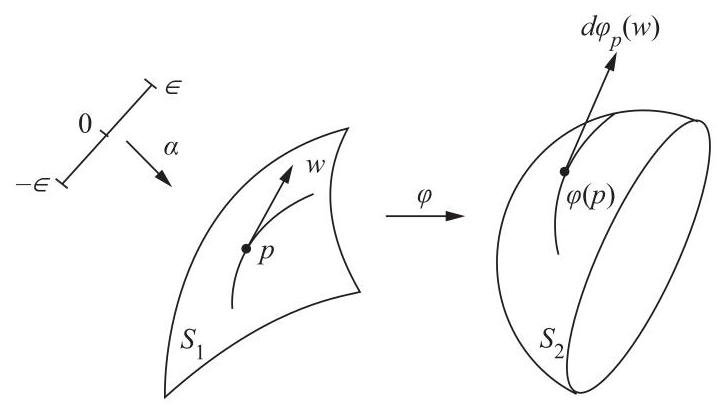
\includegraphics[max width=0.6\textwidth]{images/bo_d4b9jf3ef24c73e0334g_98_420_1019_721_408_0.jpg}
\end{center}
\hspace*{3em} 

图 2-24

命题 2. 在上述讨论中，给定 \(\mathrm{w}\) ，向量 \({\beta }^{\prime }\left( 0\right)\) 不依赖于 \(\alpha\) 的选择.由 \(\mathrm{d}{\varphi }_{\mathrm{p}}\left( \mathrm{w}\right)  = {\beta }^{\prime }\left( 0\right)\) 定义的映射 \(\mathrm{d}{\varphi }_{\mathrm{p}} : {\mathrm{T}}_{\mathrm{p}}\left( {S}_{1}\right)  \rightarrow  {\mathrm{T}}_{\varphi \left( \mathrm{p}\right) }\left( {S}_{2}\right)\) 是线性的.

证明. 证明与欧几里得空间中的证明类似(参见第 2 章附录中的命题 7).设 \(\mathbf{x}\left( {u,v}\right) ,\overline{\mathbf{x}}\left( {\bar{u},\bar{v}}\right)\) 分别是 \(p\) 和 \(\varphi \left( p\right)\) 邻域中的参数化.假设 \(\varphi\) 在这些坐标中表示为

\[
\varphi \left( {u,v}\right)  = \left( {{\varphi }_{1}\left( {u,v}\right) ,{\varphi }_{2}\left( {u,v}\right) }\right)
\]

并且 \(\alpha\) 表示为

\[
\alpha \left( t\right)  = \left( {u\left( t\right) ,v\left( t\right) }\right) ,\;t \in  \left( {-\epsilon ,\epsilon }\right) .
\]

那么 \(\beta \left( t\right)  = \left( {{\varphi }_{1}\left( {u\left( t\right) ,v\left( t\right) }\right) ,{\varphi }_{2}\left( {u\left( t\right) ,v\left( t\right) }\right) }\right)\) ，并且 \({\beta }^{\prime }\left( 0\right)\) 在基 \(\left\{  {{\overline{\mathbf{x}}}_{\bar{u}},{\overline{\mathbf{x}}}_{\bar{v}}}\right\}\) 中的表示为

\[
{\beta }^{\prime }\left( 0\right)  = \left( {\frac{\partial {\varphi }_{1}}{\partial u}{u}^{\prime }\left( 0\right)  + \frac{\partial {\varphi }_{1}}{\partial v}{v}^{\prime }\left( 0\right) ,\frac{\partial {\varphi }_{2}}{\partial u}{u}^{\prime }\left( 0\right)  + \frac{\partial {\varphi }_{2}}{\partial v}{v}^{\prime }\left( 0\right) }\right) .
\]

上述关系表明 \({\beta }^{\prime }\left( 0\right)\) 仅取决于映射 \(\varphi\) 和 \(w\) 在基 \(\left\{  {{\mathbf{x}}_{u},{x}_{v}}\right\}  .{\beta }^{\prime }\left( 0\right)\) 中的坐标 \(\left( {{u}^{\prime }\left( 0\right) ,{v}^{\prime }\left( 0\right) }\right)\) ，因此与 \(\alpha\) 无关.此外，同一关系表明

\[
{\beta }^{\prime }\left( 0\right)  = d{\varphi }_{p}\left( w\right)  = \left( \begin{array}{ll} \frac{\partial {\varphi }_{1}}{\partial u} & \frac{\partial {\varphi }_{1}}{\partial v} \\  \frac{\partial {\varphi }_{2}}{\partial u} & \frac{\partial {\varphi }_{2}}{\partial v} \end{array}\right) \left( \begin{array}{l} {u}^{\prime }\left( 0\right) \\  {v}^{\prime }\left( 0\right)  \end{array}\right) ;
\]

即， \(d{\varphi }_{p}\) 是 \({T}_{p}\left( {S}_{1}\right)\) 到 \({T}_{\varphi \left( p\right) }\left( {S}_{2}\right)\) 的一个线性映射，其在 \({T}_{p}\left( {S}_{1}\right)\) 的基 \(\left\{  {{\mathbf{x}}_{u},{\mathbf{x}}_{v}}\right\}\) 和 \({T}_{\varphi \left( p\right) }\left( {S}_{2}\right)\) 的基 \(\left\{  {{\overline{\mathbf{x}}}_{\bar{u}},{\overline{\mathbf{x}}}_{\bar{v}}}\right\}\) 中的矩阵就是上面给出的矩阵.Q.E.D.

由命题 2 定义的线性映射 \(d{\varphi }_{p}\) 称为 \(\varphi\) 在 \(p \in  {S}_{1}\) 处的微分.类似地，我们将 (可微) 函数 \(f : U \subset  S \rightarrow  R\) 在 \(p \in  U\) 处的微分定义为一个线性映射 \(d{f}_{p} : {T}_{p}\left( S\right)  \rightarrow  R\) .细节留给读者.

例 1. 设 \(v \in  {R}^{3}\) 为单位向量，设 \(h : S \rightarrow  R,h\left( p\right)  = v \cdot  p\) ， \(p \in  S\) 为第 2-3 节例 1 中定义的高度函数.为了计算 \(d{h}_{p}\left( w\right) ,w \in  {T}_{p}\left( S\right)\) ，选择一条可微曲线 \(\alpha  : \left( {-\epsilon ,\epsilon }\right)  \rightarrow  S\) ，使得 \(\alpha \left( 0\right)  = p,{\alpha }^{\prime }\left( 0\right)  = w\) .由于 \(h\left( {\alpha \left( t\right) }\right)  = \alpha \left( t\right)  \cdot  v\) ，我们得到

\[
d{h}_{p}\left( w\right)  = {\left. \frac{d}{dt}h\left( \alpha \left( t\right) \right) \right| }_{t = 0} = {\alpha }^{\prime }\left( 0\right)  \cdot  v = w \cdot  v.
\]

例 2. 设 \({S}^{2} \subset  {R}^{3}\) 为单位球面

\[
{S}^{2} = \left\{  {\left( {x,y,z}\right)  \in  {R}^{3};{x}^{2} + {y}^{2} + {z}^{2} = 1}\right\}
\]

设 \({R}_{z,\theta } : {R}^{3} \rightarrow  {R}^{3}\) 为绕 \(z\) 轴旋转 \(\theta\) 角的旋转.那么 \({R}_{z,\theta }\) 在 \({S}^{2}\) 上的限制是 \({S}^{2}\) 的一个可微映射(参见第 2-3 节例 3).我们将计算 \({\left( d{R}_{z,\theta }\right) }_{p}\left( w\right) ,p \in  {S}^{2},w \in  {T}_{p}\left( {S}^{2}\right)\) .设 \(\alpha  : \left( {-\epsilon ,\epsilon }\right)  \rightarrow  {S}^{2}\) 为一条可微曲线，使得 \(\alpha \left( 0\right)  = p,{\alpha }^{\prime }\left( 0\right)  = w\) .那么，由于 \({R}_{z,\theta }\) 是线性的，

\[
{\left( d{R}_{z,\theta }\right) }_{p}\left( w\right)  = \frac{d}{dt}{\left( {R}_{z,\theta } \circ  \alpha \left( t\right) \right) }_{t = 0} = {R}_{z,\theta }\left( {{\alpha }^{\prime }\left( 0\right) }\right)  = {R}_{z,\theta }\left( w\right) .
\]

注意到 \({R}_{z,\theta }\) 固定了北极 \(N = \left( {0,0,1}\right)\) ，并且 \({\left( d{R}_{z,\theta }\right) }_{N} : {T}_{N}\left( {S}^{2}\right)  \rightarrow  {T}_{N}\left( {S}^{2}\right)\) 是在平面 \({T}_{N}\left( {S}^{2}\right)\) 中旋转 \(\theta\) 角的旋转.

回顾起来，我们到目前为止所做的就是将 \({R}^{2}\) 中的微分演算概念推广到正则曲面.由于微积分本质上是局部理论，我们定义了一个实体(正则曲面)，该实体在局部上是平面，除了微分同胚，因此这种推广变得自然.因此，可以预期基本的反函数定理可以推广到曲面之间的可微映射.

我们称一个映射 \(\varphi  : U \subset  {S}_{1} \rightarrow  {S}_{2}\) 在 \(p \in  U\) 处是局部微分同胚，如果存在 \(p\) 的一个邻域 \(V \subset  U\) ，使得 \(\varphi\) 在 \(V\) 上的限制是一个到开集 \(\varphi \left( V\right)  \subset  {S}_{2}\) 的微分同胚.用这些术语来说，曲面反函数定理的版本表示如下.

命题 3. 如果 \({S}_{1}\) 和 \({S}_{2}\) 是正则曲面，并且 \(\varphi  : \mathrm{U} \subset  {S}_{1} \rightarrow  {S}_{2}\) 是开集 \(\mathrm{U} \subset  {S}_{1}\) 的一个可微映射，使得 \(\varphi\) 在 \(\mathrm{p} \in  \mathrm{U}\) 处的微分 \(\mathrm{d}{\varphi }_{\mathrm{p}}\) 是一个同构，那么 \(\varphi\) 在 \(\mathrm{p}\) 处是局部微分同胚.

证明是 \({R}^{2}\) 中反函数定理的一个直接应用，将留作练习.

当然，微积分的所有其他概念，如临界点、正则值等，都可以自然地推广到定义在正则曲面上的函数和映射.

切平面也允许我们讨论两条相交曲面在交点处的夹角.

给定正则曲面 \(S\) 上的点 \(p\) ，存在 \({R}^{3}\) 的两个单位向量垂直于切平面 \({T}_{p}\left( S\right)\) ；每个向量都称为 \(p\) 处的单位法向量.通过 \(p\) 且包含 \(p\) 处单位法向量的直线称为 \(p\) 处的法线.两条相交曲面在交点 \(p\) 处的夹角是它们在 \(p\) 处的切平面(或法线)的夹角(图 2-25).

\begin{center}
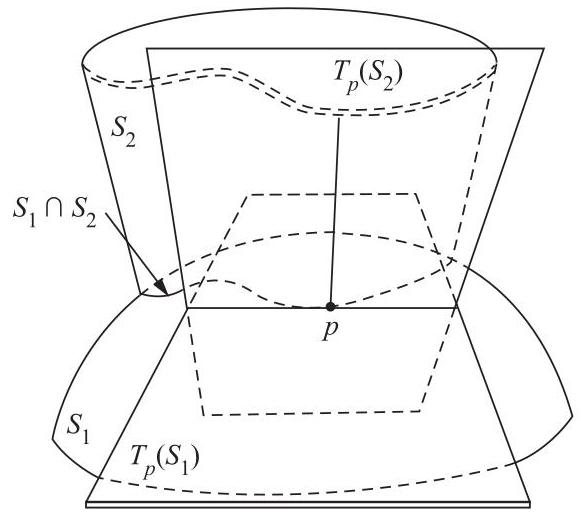
\includegraphics[max width=0.5\textwidth]{images/bo_d4b9jf3ef24c73e0334g_100_196_1394_582_518_0.jpg}
\end{center}
\hspace*{3em} 

图 2-25

通过固定 \(p \in  S\) 处的参数化 \(\mathbf{x} : U \subset  {R}^{2} \rightarrow  S\) ，我们可以根据以下规则为每个点 \(q \in  \mathbf{x}\left( U\right)\) 确定一个单位法向量.

\[
N\left( q\right)  = \frac{{\mathbf{x}}_{u} \land  {x}_{v}}{\left| {x}_{u} \land  {x}_{v}\right| }\left( q\right) .
\]

因此，我们得到一个可微映射 \(N : \mathbf{x}\left( U\right)  \rightarrow  {R}^{3}\) .我们稍后(第 2-6 节和第 3-1 节)将看到，并非总是可能将此映射可微地扩展到整个曲面 \(S\) .

在结束本节之前，我们将对可微性问题做一些观察.

正则曲面的定义要求参数化是 \({C}^{\infty }\) 类，也就是说，它们具有所有阶的连续偏导数.对于微分几何的问题，我们通常只需要直到某个阶数的偏导数存在且连续，这个阶数取决于问题的性质(很少需要超过四个导数).

例如，切平面的存在性和连续性仅取决于一阶偏导数的存在性和连续性.因此，可能出现函数 \(z = f\left( {x,y}\right)\) 的图像在每一点都存在切平面，但其可微性不足以满足正则曲面的定义.这在以下示例中会发生.

示例 3. 考虑函数 \(z = \sqrt[3]{{\left( {x}^{2} + {y}^{2}\right) }^{2}}\) 的图像，该图像是通过将曲线 \(z = {x}^{4/3}\) 绕 \(z\) 轴旋转生成的.由于该曲线相对于 \(z\) 轴对称，并且具有在原点处消失的连续导数，因此很明显 \(z = \sqrt[3]{{\left( {x}^{2} + {y}^{2}\right) }^{2}}\) 的图像在原点处以 \({xy}\) 平面作为切平面.然而，偏导数 \({z}_{xx}\) 在原点处不存在，并且所考虑的图像不是上述定义的正则曲面(参见第 2-2 节的命题 3).

我们不打算深入研究这类问题.定义中的假设 \({C}^{\infty }\) 正是为了避免研究每种特定情况所需的最小可微性条件.这些细微之处有其存在的意义，但它们最终可能会模糊此处处理问题的几何性质.

\exerciseline

*1. 证明在正则曲面 \(f\left( {x,y,z}\right)  = 0\) 的 \(\left( {{x}_{0},{y}_{0},{z}_{0}}\right)\) 处的切平面方程为，其中 0 是 \(f\) 的正则值:

\[
{f}_{x}\left( {{x}_{0},{y}_{0},{z}_{0}}\right) \left( {x - {x}_{0}}\right)  + {f}_{y}\left( {{x}_{0},{y}_{0},{z}_{0}}\right) \left( {y - {y}_{0}}\right)  + {f}_{z}\left( {{x}_{0},{y}_{0},{z}_{0}}\right) \left( {z - {z}_{0}}\right)
\]

\[
= 0\text{ . }
\]

2. 确定 \({x}^{2} + {y}^{2} - {z}^{2} = 1\) 在点 \(\left( {x,y,0}\right)\) 处的切平面，并证明它们都平行于 \(z\) 轴.

3. 证明可微函数 \(z = f\left( {x,y}\right)\) 的图像曲面在点 \({p}_{0} = \left( {{x}_{0},{y}_{0}}\right)\) 处的切平面方程为:

\[
z = f\left( {{x}_{0},{y}_{0}}\right)  + {f}_{x}\left( {{x}_{0},{y}_{0}}\right) \left( {x - {x}_{0}}\right)  + {f}_{y}\left( {{x}_{0},{y}_{0}}\right) \left( {y - {y}_{0}}\right) .
\]

回顾函数 \(f : {R}^{2} \rightarrow  R\) 的微分 \({df}\) 的定义，并证明切平面是微分 \(d{f}_{p}\) 的图像.

*4. 证明由 \(z = {xf}\left( {y/x}\right) ,x \neq  0\) 给出的曲面，其中 \(f\) 是可微函数，其所有切平面都通过原点 \(\left( {0,0,0}\right)\) .

5. 如果正则曲面的一个坐标邻域可以参数化为

\[
\mathbf{x}\left( {u,v}\right)  = {\alpha }_{1}\left( u\right)  + {\alpha }_{2}\left( v\right) ,
\]

其中 \({\alpha }_{1}\) 和 \({\alpha }_{2}\) 是正则参数化曲线，证明该邻域沿固定坐标曲线的切平面都平行于某条直线.

6. 令 \(\alpha  : I \rightarrow  {R}^{3}\) 为具有处处非零曲率的正则参数化曲线.考虑 \(\alpha\) 的切面(第 2-3 节示例 5)

\[
\mathbf{x}\left( {t,v}\right)  = \alpha \left( t\right)  + v{\alpha }^{\prime }\left( t\right) ,\;t \in  I,v \neq  0.
\]

证明沿曲线 \(\mathbf{x}\left( {\text{ const., }v}\right)\) 的切平面都相等.

7. 令 \(f : S \rightarrow  R\) 由 \(f\left( p\right)  = {\left| p - {p}_{0}\right| }^{2}\) 给出，其中 \(p \in  S\) 和 \({p}_{0}\) 是 \({R}^{3}\) 的固定点(参见第 2-3 节示例 1).证明 \(d{f}_{p}\left( w\right)  = \; {2w} \cdot  \left( {p - {p}_{0}}\right) ,w \in  {T}_{p}\left( S\right) .\)

8. 证明如果 \(L : {R}^{3} \rightarrow  {R}^{3}\) 是线性映射，而 \(S \subset  {R}^{3}\) 是在 \(L\) 下不变的正则曲面，即 \(L\left( S\right)  \subset  S\) ，那么限制 \(L \mid  S\) 是可微映射，并且

\[
d{L}_{p}\left( w\right)  = L\left( w\right) ,\;p \in  S,w \in  {T}_{p}\left( S\right) .
\]

9. 证明参数化曲面

\[
x\left( {u,v}\right)  = \left( {v\cos u,v\sin u,{au}}\right) ,\;a \neq  0,
\]

是正则的.计算其法向量 \(N\left( {u,v}\right)\) ，并证明沿坐标线 \(u = {u}_{0}\) ，曲面 \(\mathbf{x}\) 的切平面绕此线旋转，使其与 \(z\) 轴夹角的正切值与点 \(\mathbf{x}\left( {{u}_{0},v}\right)\) 到 \(\mathrm{z}\) 轴的距离 \(v\left( { = \sqrt{{x}^{2} + {y}^{2}}}\right)\) 的倒数成正比.

10. (管状曲面.) 设 \(\alpha  : I \rightarrow  {R}^{3}\) 为一条处处曲率非零且以弧长为参数的正则参数化曲线.设

\[
\mathbf{x}\left( {s,v}\right)  = \alpha \left( s\right)  + r\left( {n\left( s\right) \cos v + b\left( s\right) \sin v}\right) ,\;r = \text{ const. } \neq  0,s \in  I,
\]

为参数化曲面(围绕 \(\alpha\) 的半径为 \(r\) 的管)，其中 \(n\) 是 \(\alpha\) 的法向量， \(b\) 是 \(\alpha\) 的副法向量.证明当 \(\mathbf{x}\) 是正则的时，其单位法向量为

\[
N\left( {s,v}\right)  =  - \left( {n\left( s\right) \cos v + b\left( s\right) \sin v}\right) .
\]

11. 证明由以下参数化曲面给出的法线

\[
\mathbf{x}\left( {u,v}\right)  = \left( {f\left( u\right) \cos v,f\left( u\right) \sin v,g\left( u\right) }\right) ,\;f\left( u\right)  \neq  0,{g}^{\prime } \neq  0,
\]

都通过 \(z\) 轴.

*12. 证明每个方程 \(\left( {a,b,c \neq  0}\right)\)

\[
{x}^{2} + {y}^{2} + {z}^{2} = {ax}
\]

\[
{x}^{2} + {y}^{2} + {z}^{2} = {by}
\]

\[
{x}^{2} + {y}^{2} + {z}^{2} = {cz}
\]

定义了一个正则曲面，并且它们都相互正交.

13. 定义在正则曲面 \(S\) 上的可微函数 \(f : S \rightarrow  R\) 的临界点是点 \(p \in  S\) ，使得 \(d{f}_{p} = 0\) .

*a. 设 \(f : S \rightarrow  R\) 由 \(f\left( p\right)  = \left| {p - {p}_{0}}\right| ,p \in  S,{p}_{0} \notin  S\) (参见习题 5, 第 2-3 节)给出.证明 \(p \in  S\) 是 \(f\) 的临界点当且仅当连接 \(p\) 和 \({p}_{0}\) 的直线在 \(p\) 处垂直于 \(S\) .

b. 令 \(h : S \rightarrow  R\) 由 \(h\left( p\right)  = p \cdot  v\) 给出，其中 \(v \in  {R}^{3}\) 是单位向量(参见示例 1，第 2-3 节).证明 \(p \in  S\) 是 \(f\) 的临界点当且仅当 \(v\) 是 \(S\) 在 \(p\) 处的法向量.

*14. 设 \(Q\) 是三个坐标平面 \(x = 0,y = 0,z = 0\) 的并集.设 \(p = \left( {x,y,z}\right)  \in  {R}^{3} - Q\) .

a. 证明 \(t\) 中的方程

\[
\frac{{x}^{2}}{a - t} + \frac{{y}^{2}}{b - t} + \frac{{z}^{2}}{c - t} \equiv  f\left( t\right)  = 1,\;a > b > c > 0,
\]

有三个不同的实根: \({t}_{1},{t}_{2},{t}_{3}\) .

b. 证明对于每个 \(p \in  {R}^{3} - Q\) ，由 \(f\left( {t}_{1}\right)  - 1 = 0\) 和 \(f\left( {t}_{2}\right)  - 1 = 0,f\left( {t}_{3}\right)  - 1 = 0\) 给出的集合是经过 \(p\) 的正则曲面，并且它们两两正交.

15. 证明如果一个连通曲面的所有法线都通过一个固定点，则该曲面包含在一个球体中.

16. 设 \(w\) 是正则曲面 \(S\) 在点 \(p \in  S\) 处的切向量，设 \(\mathbf{x}\left( {u,v}\right)\) 和 \(\overline{\mathbf{x}}\left( {\bar{u},\bar{v}}\right)\) 是 \(p\) 的两个参数化.假设 \(w\) 在与 \(\mathbf{x}\left( {u,v}\right)\) 和 \(\overline{\mathbf{x}}\left( {\bar{u},\bar{v}}\right)\) 相关的基下的表达式为

\[
w = {\alpha }_{1}{\mathbf{x}}_{u} + {\alpha }_{2}{\mathbf{x}}_{v}
\]

和

\[
w = {\beta }_{1}{\overline{\mathbf{x}}}_{\bar{u}} + {\beta }_{2}{\mathbf{x}}_{\bar{v}}.
\]

证明 \(w\) 的坐标满足关系

\[
{\beta }_{1} = {\alpha }_{1}\frac{\partial \bar{u}}{\partial u} + {\alpha }_{2}\frac{\partial \bar{u}}{\partial v}
\]

\[
{\beta }_{2} = {\alpha }_{1}\frac{\partial \bar{v}}{\partial u} + {\alpha }_{2}\frac{\partial \bar{v}}{\partial v}
\]

其中 \(\bar{u} = \bar{u}\left( {u,v}\right)\) 和 \(\bar{v} = \bar{v}\left( {u,v}\right)\) 是坐标变换的表达式.

*17. 两个正则曲面 \({S}_{1}\) 和 \({S}_{2}\) 横截相交，如果当 \(p \in  {S}_{1} \cap  {S}_{2}\) 时， \({T}_{p}\left( {S}_{1}\right)  \neq  {T}_{p}\left( {S}_{2}\right)\) .证明如果 \({S}_{1}\) 与 \({S}_{2}\) 横截相交，则 \({S}_{1} \cap  {S}_{2}\) 是一个正则曲线.

18. 证明如果一个正则曲面 \(S\) 在一个点 \(p\) 处与平面 \(P\) 相交，则该平面与 \(S\) 在 \(p\) 处的切平面重合.

19. 设 \(S \subset  {R}^{3}\) 为一个规则曲面， \(P \subset  {R}^{3}\) 为一个平面.若 \(S\) 的所有点都在 \(P\) 的同一侧，证明 \(P\) 在 \(P \cap  S\) 的所有点上都与 \(S\) 相切.

*20. 证明椭球 \(\left( {0,0,0}\right)\) 的中心的垂直投影

\[
\frac{{x}^{2}}{{a}^{2}} + \frac{{y}^{2}}{{b}^{2}} + \frac{{z}^{2}}{{c}^{2}} = 1
\]

到其切平面上构成一个由下式给出的正则曲面

\[
\left\{  {\left( {x,y,z}\right)  \in  {R}^{3};{\left( {x}^{2} + {y}^{2} + {z}^{2}\right) }^{2} = {a}^{2}{x}^{2} + {b}^{2}{y}^{2} + {c}^{2}{z}^{2}}\right\}   - \{ \left( {0,0,0}\right) \} .
\]

*21. 设 \(f : S \rightarrow  R\) 是连通正则曲面 \(S\) 上的一个可微函数.假设对于所有 \(p \in  S\) ， \(d{f}_{p} = 0\) .证明 \(f\) 在 \(S\) 上是常数.

*22. 证明:如果一个连通正则曲面 \(S\) 的所有法线都交于一条定直线，则 \(S\) 是一个旋转曲面片.

23. 证明:在 2-3 节练习 16 中定义的映射 \(F : {S}^{2} \rightarrow  {S}^{2}\) 只有有限个临界点(见练习 13).

24. (链式法则.)证明:如果 \(\varphi  : {S}_{1} \rightarrow  {S}_{2}\) 和 \(\psi  : {S}_{2} \rightarrow  {S}_{3}\) 是可微映射，且 \(p \in  {S}_{1}\) ，则

\[
d{\left( \psi  \circ  \varphi \right) }_{p} = d{\psi }_{\varphi \left( p\right) } \circ  d{\varphi }_{p}.
\]

25. 证明:如果一个正则曲面 \(S\) 上的两条正则曲线 \({C}_{1}\) 和 \({C}_{2}\) 在点 \(p \in  S\) 处相切，并且 \(\varphi  : S \rightarrow  S\) 是一个微分同胚，则 \(\varphi \left( {C}_{1}\right)\) 和 \(\varphi \left( {C}_{2}\right)\) 是正则曲线，且在 \(\varphi \left( p\right)\) 处相切.

26. 证明:如果 \(p\) 是正则曲面 \(S\) 上的一个点，通过方便地选取 \(\left( {x,y,z}\right)\) 坐标，可以表示 \(S\) 在 \(p\) 附近的一个邻域为 \(z = f\left( {x,y}\right)\) 的形式，使得 \(f\left( {0,0}\right)  = 0,{f}_{x}\left( {0,0}\right)  = 0\) ， \({f}_{y}\left( {0,0}\right)  = 0\) .(这等价于将 \(S\) 在 \(p\) 处的切平面取为 \({xy}\) 平面.)

27. (接触理论.)在 \({R}^{3}\) 中的两个正则曲面 \(S\) 和 \(\bar{S}\) ，如果它们有一个公共点 \(p\) ，则称它们在 \(p\) 处具有 \(\geq  1\) 阶接触，如果存在参数化，它们在 \(p\) 处具有相同的定义域 \(\mathbf{x}\left( {u,v}\right) ,\overline{\mathbf{x}}\left( {u,v}\right)\) ，分别是 \(S\) 和 \(\bar{S}\) 的，使得 \({\mathbf{x}}_{u} = {\overline{\mathbf{x}}}_{u}\) 且在 \(p\) 处 \({\mathbf{x}}_{v} = {\overline{\mathbf{x}}}_{v}\) .如果此外，在 \(p\) 处某些二阶偏导数不同，则称接触的阶数恰好等于 1.证明:

a. 正则曲面 \(S\) 在点 \(p\) 处的切平面 \({T}_{p}\left( S\right)\) 在 \(p\) 处与该曲面具有 \(\geq  1\) 阶接触.

b. 如果一个平面在 \(p\) 处与曲面 \(S\) 具有 \(\geq  1\) 阶接触，则该平面与 \(S\) 在 \(p\) 处的切平面重合.

c. 两个正则曲面具有 \(\geq  1\) 阶接触当且仅当它们在 \(p\) 处有共同的切平面，即它们在 \(p\) 处相切.

d. 如果 \({R}^{3}\) 中的两个正则曲面 \(S\) 和 \(\bar{S}\) 在 \(p\) 处具有 \(\geq  1\) 阶接触，并且 \(F : {R}^{3} \rightarrow  {R}^{3}\) 是 \({R}^{3}\) 的一个微分同胚，则像 \(F\left( S\right)\) 和 \(F\left( \bar{S}\right)\) 是正则曲面，并且在 \(f\left( p\right)\) 处具有 \(\geq  1\) 阶接触(即， \(\geq  1\) 阶接触的概念在微分同胚下是不变的).

e. 如果两个曲面在 \(p\) 处具有 \(\geq  1\) 阶接触，则 \(\mathop{\lim }\limits_{{r \rightarrow  0}}\left( {d/r}\right)  = 0\) ，其中 \(d\) 是由平行于公共法线的直线与曲面的交点所确定的线段的长度，该直线距离该法线 \(r\) .

28. a. 定义正则曲面 \(S\) 上可微函数 \(f : S \rightarrow  R\) 的正则值.

b. 证明正则曲面 \(S\) 上可微函数的正则值的逆像是 \(S\) 上的正则曲线.

\section*{2-5. 第一基本形式；面积}

到目前为止，我们从可微性的角度考察了曲面.在本节中，我们将开始研究曲面所承载的进一步几何结构.其中最重要的是第一基本形式，我们现在将对其进行描述.

\({R}^{3} \supset  S\) 的自然内积在正则曲面 \(S\) 的每个切平面 \({T}_{p}\left( S\right)\) 上诱导出一个内积，记为 \(\langle ,{\rangle }_{p}\) :如果 \({w}_{1},{w}_{2} \in  {T}_{p}\left( S\right)  \subset  {R}^{3}\) ，则 \({\left\langle  {w}_{1},{w}_{2}\right\rangle  }_{p}\) 等于 \({w}_{1}\) 和 \({w}_{2}\) 在 \({R}^{3}\) 中的向量内积.对于这个内积，它是一个对称双线性形式(即， \(\left\langle  {{w}_{1},{w}_{2}}\right\rangle   = \left\langle  {{w}_{2},{w}_{1}}\right\rangle\) 且 \(\left\langle  {{w}_{1},{w}_{2}}\right\rangle\) 在 \({w}_{1}\) 和 \({w}_{2}\) 中都是线性的)，对应一个二次型 \({I}_{p} : {T}_{p}\left( S\right)  \rightarrow  R\) ，其定义为

\[
{I}_{p}\left( w\right)  = \langle w,w{\rangle }_{p} = {\left| w\right| }^{2} \geq  0. \tag{1}
\]

定义 1. 由式 (1) 定义的 \({\mathrm{T}}_{\mathrm{p}}\left( S\right)\) 上的二次型 \({\mathrm{I}}_{\mathrm{p}}\) ，称为曲面 \(S \subset  {R}^{3}\) 在 \(\mathrm{p} \in  S\) 处的第一基本形式.

因此，第一基本形式仅仅是曲面 \(S\) 如何继承 \({R}^{3}\) 的自然内积的表达.几何上，正如我们稍后将看到的，第一基本形式使我们能够在曲面上进行测量(曲线长度、切向量夹角、区域面积)，而无需参考曲面所在的外部空间 \({R}^{3}\) .

现在我们将第一基本形式表示为与参数化 \(\mathbf{x}\left( {u,v}\right)\) 在 \(p\) 处相关的基 \(\left\{  {{\mathbf{x}}_{u},{\mathbf{x}}_{v}}\right\}\) .由于切向量 \(w \in  {T}_{p}\left( S\right)\) 是参数化曲线 \(\alpha \left( t\right)  = \mathbf{x}\left( {u\left( t\right) ,v\left( t\right) }\right) ,t \in  \left( {-\epsilon ,\epsilon }\right)\) 的切向量，其中 \(p = \alpha \left( 0\right)  = \mathbf{x}\left( {{u}_{0},{v}_{0}}\right)\) ，我们得到

\[
{I}_{p}\left( {{\alpha }^{\prime }\left( 0\right) }\right)  = {\left\langle  {\alpha }^{\prime }\left( 0\right) ,{\alpha }^{\prime }\left( 0\right) \right\rangle  }_{p}
\]

\[
= {\left\langle  {\mathbf{x}}_{u}{u}^{\prime } + {\mathbf{x}}_{v}{v}^{\prime },{\mathbf{x}}_{u}{u}^{\prime } + {\mathbf{x}}_{v}{v}^{\prime }\right\rangle  }_{p}
\]

\[
= {\left\langle  {\mathbf{x}}_{u},{\mathbf{x}}_{u}\right\rangle  }_{p}{\left( {u}^{\prime }\right) }^{2} + 2{\left\langle  {\mathbf{x}}_{u},{\mathbf{x}}_{v}\right\rangle  }_{p}{u}^{\prime }{v}^{\prime } + {\left\langle  {\mathbf{x}}_{v},{\mathbf{x}}_{v}\right\rangle  }_{p}{\left( {v}^{\prime }\right) }^{2}
\]

\[
= E{\left( {u}^{\prime }\right) }^{2} + {2F}{u}^{\prime }{v}^{\prime } + G{\left( {v}^{\prime }\right) }^{2},
\]

其中所涉及函数的取值是针对 \(t = 0\) 计算的，并且

\[
E\left( {{u}_{0},{v}_{0}}\right)  = {\left\langle  {\mathbf{x}}_{u},{\mathbf{x}}_{u}\right\rangle  }_{p},
\]

\[
F\left( {{u}_{0},{v}_{0}}\right)  = {\left\langle  {\mathbf{x}}_{u},{\mathbf{x}}_{v}\right\rangle  }_{p},
\]

\[
G\left( {{u}_{0},{v}_{0}}\right)  = {\left\langle  {\mathbf{x}}_{v},{\mathbf{x}}_{v}\right\rangle  }_{p}
\]

是 \({T}_{p}\left( S\right)\) 基 \(\left\{  {{\mathbf{x}}_{u},{\mathbf{x}}_{v}}\right\}\) 下的一阶基本形式的系数.通过让 \(p\) 在对应于 \(\mathbf{x}\left( {u,v}\right)\) 的坐标邻域中变化，我们得到在邻域中可微的函数 \(E\left( {u,v}\right) ,F\left( {u,v}\right) ,G\left( {u,v}\right)\) .

从现在开始，当上下文清楚我们指的是哪个点时，我们将省略内积 \(\langle\) 、 \({\rangle }_{p}\) 或二次型 \({I}_{p}\) 表示中的下标 \(p\) .为了方便起见，我们还将用相同的符号 \(\langle\) 、 \(\rangle {ratherthanthepreviousdot}\) 来表示 \({R}^{3}\) 的自然内积.

例 1. 通过 \({p}_{0} = \left( {{x}_{0},{y}_{0},{z}_{0}}\right)\) 并包含正交向量 \({w}_{1} = \left( {{a}_{1},{a}_{2},{a}_{3}}\right)\) 、 \({w}_{2} = \left( {{b}_{1},{b}_{2},{b}_{3}}\right)\) 的平面 \(P \subset  {R}^{3}\) 的坐标系如下:

\[
\mathbf{x}\left( {u,v}\right)  = {p}_{0} + u{w}_{1} + v{w}_{2},\;\left( {u,v}\right)  \in  {R}^{2}.
\]

为了计算 \(P\) 的任意一点的一阶基本形式，我们注意到 \({\mathbf{x}}_{u} = {w}_{1},{\mathbf{x}}_{v} = {w}_{2}\) ；因为 \({w}_{1}\) 和 \({w}_{2}\) 是单位正交向量，函数 \(E,F,G\) 是常数，并由下式给出:

\[
E = 1,\;F = 0,\;G = 1.
\]

在这种平凡的情况下，一阶基本形式本质上是 \(P\) 中的勾股定理；即，向量 \(w\) 在基 \(\left\{  {{\mathbf{x}}_{u},{\mathbf{x}}_{v}}\right\}\) 中的坐标为 \(a,b\) ，其长度的平方等于 \({a}^{2} + {b}^{2}\) .

例 2. 圆 \({x}^{2} + {y}^{2} = 1\) 上的直圆柱体允许参数化 \(\mathbf{x} : U \rightarrow  {R}^{3}\) ，其中(图 2-26)

\[
\mathbf{x}\left( {u,v}\right)  = \left( {\cos u,\sin u,v}\right) ,
\]

\[
U = \left\{  {\left( {u,v}\right)  \in  {R}^{2};\;0 < u < {2\pi },\; - \infty  < v < \infty }\right\}  .
\]

\begin{center}
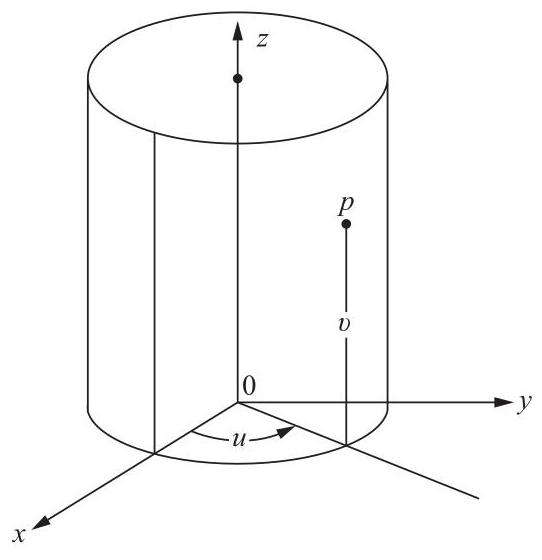
\includegraphics[max width=0.4\textwidth]{images/bo_d4b9jf3ef24c73e0334g_107_180_716_542_560_0.jpg}
\end{center}
\hspace*{3em} 

图 2-26

为了计算一阶基本形式，我们注意到:

\[
{\mathbf{x}}_{u} = \left( {-\sin u,\cos u,0}\right) ,\;{\mathbf{x}}_{v} = \left( {0,0,1}\right) ,
\]

因此:

\[
E = {\sin }^{2}u + {\cos }^{2}u = 1,\;F = 0,\;G = 1.
\]

我们注意到，尽管圆柱体和平面是不同的曲面，但我们在两种情况下都得到了相同的结果.稍后我们将回到这个主题(第 4-2 节).

例 3. 考虑一个螺旋线，其方程为(参见第 1-2 节例 1)(cos \(u\) , sin \(u\) , au).通过螺旋线上的每一点，画一条平行于 \({xy}\) 平面并与 \(z\) 轴相交的直线.由这些直线生成的曲面称为螺旋面，其参数化如下:

\[
\mathbf{x}\left( {u,v}\right)  = \left( {v\cos u,v\sin u,{au}}\right) ,\;0 < u < {2\pi },\; - \infty  < v < \infty .
\]

\(\mathbf{x}\) 将 \({uv}\) 平面上宽度为 \({2\pi }\) 的开放条带映射到螺旋面上对应于螺旋线 \({2\pi }\) 旋转的部分(图 2-27).

\begin{center}
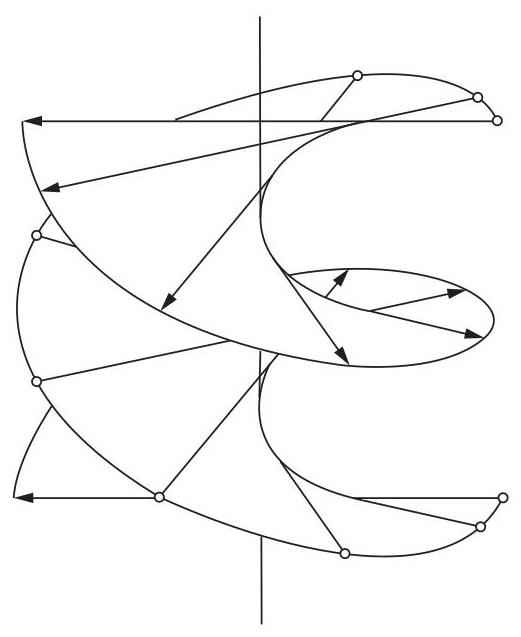
\includegraphics[max width=0.4\textwidth]{images/bo_d4b9jf3ef24c73e0334g_108_196_189_521_637_0.jpg}
\end{center}
\hspace*{3em} 

图 2-27. 螺旋面.

验证螺旋面是正则曲面是直接的，留给读者完成.

计算上述参数化中一阶基本形式的系数得到:

\[
E\left( {u,v}\right)  = {v}^{2} + {a}^{2},\;F\left( {u,v}\right)  = 0,\;G\left( {u,v}\right)  = 1.
\]

正如我们之前提到的，一阶基本形式 \(I\) 的重要性在于，通过了解 \(I\) ，我们可以处理正则曲面上的度量问题，而无需进一步参考环境空间 \({R}^{3}\) .因此，参数化曲线 \(\alpha  : I \rightarrow  S\) 的弧长 \(s\) 由下式给出:

\[
s\left( t\right)  = {\int }_{o}^{t}\left| {{\alpha }^{\prime }\left( t\right) }\right| {dt} = {\int }_{o}^{t}\sqrt{I\left( {{\alpha }^{\prime }\left( t\right) }\right) }{dt}.
\]

特别地，如果 \(\alpha \left( t\right)  = \mathbf{x}\left( {u\left( t\right) ,v\left( t\right) }\right)\) 包含在与参数化 \(\mathbf{x}\left( {u,v}\right)\) 对应的坐标邻域中，我们可以计算 \(\alpha\) 在 0 和 \(t\) 之间的弧长，例如，通过

\[
s\left( t\right)  = {\int }_{0}^{t}\sqrt{E{\left( {u}^{\prime }\right) }^{2} + {2F}{u}^{\prime }{v}^{\prime } + G{\left( {v}^{\prime }\right) }^{2}}{dt}. \tag{2}
\]

此外，两条参数化正则曲线 \(\alpha  : I \rightarrow  S\) , \(\beta  : I \rightarrow  S\) 在 \(t = {t}_{0}\) 相交的角度 \(\theta\) 由下式给出

\[
\cos \theta  = \frac{\left\langle  {\alpha }^{\prime }\left( {t}_{0}\right) ,{\beta }^{\prime }\left( {t}_{0}\right) \right\rangle  }{\left| {{\alpha }^{\prime }\left( {t}_{0}\right) }\right| \left| {{\beta }^{\prime }\left( {t}_{0}\right) }\right| }.
\]

特别地，参数化 \(\mathbf{x}\left( {u,v}\right)\) 的坐标曲线的角度 \(\varphi\) 为

\[
\cos \varphi  = \frac{\left\langle  {\mathbf{x}}_{u},{\mathbf{x}}_{v}\right\rangle  }{\left| {\mathbf{x}}_{u}\right| \left| {\mathbf{x}}_{v}\right| } = \frac{F}{\sqrt{EG}};
\]

由此可知，参数化的坐标曲线正交当且仅当对于所有 \(\left( {\mathrm{u},\mathrm{v}}\right)\) 都有 \(\mathrm{F}\left( {\mathrm{u},\mathrm{v}}\right)  = 0\) .这样的参数化称为正交参数化.

注.由于公式 (2)，许多数学家谈论弧长“元素”， \(S\) 的 \({ds}\) ，并写道

\[
d{s}^{2} = {Ed}{u}^{2} + {2Fdudv} + {Gd}{v}^{2},
\]

表示如果 \(\alpha \left( t\right)  = \mathbf{x}\left( {u\left( t\right) ,v\left( t\right) }\right)\) 是 \(S\) 上的曲线，而 \(s = s\left( t\right)\) 是其弧长，则

\[
{\left( \frac{ds}{dt}\right) }^{2} = E{\left( \frac{du}{dt}\right) }^{2} + {2F}\frac{du}{dt}\frac{dv}{dt} + G{\left( \frac{dv}{dt}\right) }^{2}.
\]

例 4.我们将计算球面上一点的第一个基本形式，该点位于由参数化给出的坐标邻域中(参见例 1，第 2-2 节)

\[
\mathbf{x}\left( {\theta ,\varphi }\right)  = \left( {\sin \theta \cos \varphi ,\sin \theta \sin \varphi ,\cos \theta }\right) .
\]

首先，观察到

\[
{\mathbf{x}}_{\theta }\left( {\theta ,\varphi }\right)  = \left( {\cos \theta \cos \varphi ,\cos \theta \sin \varphi , - \sin \theta }\right) ,
\]

\[
{\mathbf{x}}_{\varphi }\left( {\theta ,\varphi }\right)  = \left( {-\sin \theta \sin \varphi ,\sin \theta \cos \varphi ,0}\right) .
\]

因此，

\[
E\left( {\theta ,\varphi }\right)  = \left\langle  {{\mathbf{x}}_{\theta },{\mathbf{x}}_{\theta }}\right\rangle   = 1,
\]

\[
F\left( {\theta ,\varphi }\right)  = \left\langle  {{\mathbf{x}}_{\theta },{\mathbf{x}}_{\varphi }}\right\rangle   = 0,
\]

\[
G\left( {\theta ,\varphi }\right)  = \left\langle  {{\mathbf{x}}_{\varphi },{\mathbf{x}}_{\varphi }}\right\rangle   = {\sin }^{2}\theta .
\]

因此，如果 \(w\) 是球面上点 \(\mathbf{x}\left( {\theta ,\varphi }\right)\) 的切向量，在与 \(\mathbf{x}\left( {\theta ,\varphi }\right)\) 相关的基中由下式给出

\[
w = a{\mathbf{x}}_{\theta } + b{\mathbf{x}}_{\varphi },
\]

则 \(w\) 长度的平方由下式给出

\[
{\left| w\right| }^{2} = I\left( w\right)  = E{a}^{2} + {2Fab} + G{b}^{2} = {a}^{2} + {b}^{2}{\sin }^{2}\theta .
\]

作为应用，让我们确定球面上此坐标邻域中与经线 \(\varphi  =\) const. 成恒定角度 \(\beta\) 的曲线.这些曲线称为球面的等角线(或称恒向线).

我们可以假设所需的曲线 \(\alpha \left( t\right)\) 是 \(\mathbf{x}\) 在 \({\theta \varphi }\) 平面上的一条曲线 \(\left( {\theta \left( t\right) ,\varphi \left( t\right) }\right)\) 的像.在曲线与经线 \(\varphi  =\) const. 相交的点 \(\mathbf{x}\left( {\theta ,\varphi }\right)\) 处，我们有

\[
\cos \beta  = \frac{\left\langle  {\mathbf{x}}_{\theta },{\alpha }^{\prime }\left( t\right) \right\rangle  }{\left| {\mathbf{x}}_{\theta }\right| \left| {{\alpha }^{\prime }\left( t\right) }\right| } = \frac{{\theta }^{\prime }}{\sqrt{{\left( {\theta }^{\prime }\right) }^{2} + {\left( {\varphi }^{\prime }\right) }^{2}{\sin }^{2}\theta }},
\]

因为在基 \(\left\{  {{\mathbf{x}}_{\theta },{\mathbf{x}}_{\varphi }}\right\}\) 中，向量 \({\alpha }^{\prime }\left( t\right)\) 的坐标为 \(\left( {{\theta }^{\prime },{\varphi }^{\prime }}\right)\) ，向量 \({\mathbf{x}}_{\theta }\) 的坐标为 \(\left( {1,0}\right)\) .由此可知

\[
{\left( {\theta }^{\prime }\right) }^{2}{\tan }^{2}\beta  - {\left( {\varphi }^{\prime }\right) }^{2}{\sin }^{2}\theta  = 0
\]

or

\[
\frac{{\theta }^{\prime }}{\sin \theta } =  \pm  \frac{{\varphi }^{\prime }}{\tan \beta }
\]

因此，通过积分，我们得到等角线的方程

\[
\log \tan \left( \frac{\theta }{2}\right)  =  \pm  \left( {\varphi  + c}\right) \operatorname{cotan}\beta ,
\]

其中积分常数 \(c\) 由通过曲线的一点 \(\mathbf{x}\left( {{\theta }_{0},{\varphi }_{0}}\right)\) 来确定.

另一个度量问题，可以用第一基本形式来处理，就是计算(或定义)一个正则曲面 \(S\) 的有界区域的面积.一个(正则)区域 \(S\) 是 \(S\) 的一个开且连通的子集，其边界是正则(即其微分非零)可微同胚映射在 \(S\) 中一个圆的像，除了有限个点外.一个 \(S\) 的区域是该区域与其边界的并集(图 2-28).一个 \(S \subset  {R}^{3}\) 的区域是有界的，如果它包含在 \({R}^{3}\) 的某个球内.

\begin{center}
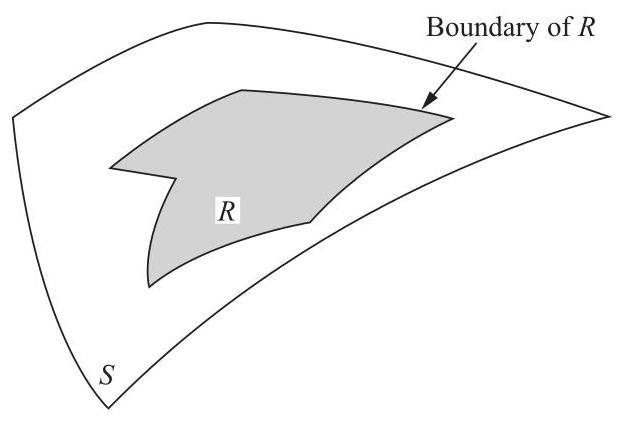
\includegraphics[max width=0.5\textwidth]{images/bo_d4b9jf3ef24c73e0334g_110_197_1687_621_422_0.jpg}
\end{center}
\hspace*{3em} 

图 2-28

设 \(Q\) 是 \({\mathbb{R}}^{2}\) 中的一个紧致区域，它包含在坐标邻域 \(\mathbf{x} : U \rightarrow  S\) 中.那么 \(\mathbf{x}\left( Q\right)  = R\) 是 \(S\) 中的一个有界区域.

函数 \(\left| {{\mathbf{x}}_{u} \land  {\mathbf{x}}_{v}}\right|\) 在 \(U\) 中定义，它测量由向量 \({\mathbf{x}}_{u}\) 和 \({\mathbf{x}}_{v}\) 生成的平行四边形的面积.我们首先证明积分

\[
{\int }_{Q}\left| {{\mathbf{x}}_{u} \land  {\mathbf{x}}_{v}}\right| {dudv}
\]

不依赖于参数化 \(\mathbf{x}\) .

事实上，设 \(\overline{\mathbf{x}} : \bar{U} \subset  {R}^{2} \rightarrow  S\) 是另一个参数化，具有 \(R \subset  \overline{\mathbf{x}}\left( \bar{U}\right)\) ，并设 \(\bar{Q} = {\overline{\mathbf{x}}}^{-1}\left( R\right)\) .设 \(\partial \left( {u,v}\right) /\partial \left( {\bar{u},\bar{v}}\right)\) 是参数变换 \(h = {\mathbf{x}}^{-1} \circ  \overline{\mathbf{x}}\) 的雅可比行列式.那么

\[
{\iint }_{\bar{Q}}\left| {{\overline{\mathbf{x}}}_{\bar{u}} \land  {\overline{\mathbf{x}}}_{\bar{v}}}\right| d\bar{u}d\bar{v} = {\iint }_{\bar{Q}}\left| {{\mathbf{x}}_{u} \land  {\mathbf{x}}_{v}}\right| \left| \frac{\partial \left( {u,v}\right) }{\partial \left( {\bar{u},\bar{v}}\right) }\right| d\bar{u}d\bar{v}
\]

\[
= {\iint }_{Q}\left| {{\mathbf{x}}_{u} \land  {\mathbf{x}}_{v}}\right| {dudv}
\]

其中最后一个等式来自多重积分中的变量替换定理(参见 Buck 高等微积分，第 304 页).因此，所声称的独立性得到了证明，我们可以给出以下定义.

定义 2. 设 \(\mathbb{R} \subset  S\) 是一个正则曲面上的有界区域，包含在参数化 \(\mathbf{x} : \mathrm{U} \subset  {\mathbb{R}}^{2} \rightarrow  S\) 的坐标邻域内.正数

\[
{\iint }_{Q}\left| {{\mathbf{x}}_{u} \land  {\mathbf{x}}_{v}}\right| \mathrm{{du}}\mathrm{{dv}} = \mathrm{A}\left( \mathbb{R}\right) ,\;\mathrm{Q} = {\mathbf{x}}^{-1}\left( \mathbb{R}\right) ,
\]

称为 \(\mathbb{R}\) 的面积.

这种定义有几种几何上的解释，其中一种将在第 2-8 节中介绍.

方便地观察到

\[
{\left| {\mathbf{x}}_{u} \land  {\mathbf{x}}_{v}\right| }^{2} + {\left\langle  {\mathbf{x}}_{u} \cdot  {\mathbf{x}}_{v}\right\rangle  }^{2} = {\left| {\mathbf{x}}_{u}\right| }^{2} \cdot  {\left| {\mathbf{x}}_{v}\right| }^{2},
\]

这表明 \(A\left( R\right)\) 的被积函数可以写成

\[
\left| {{\mathbf{x}}_{u} \land  {\mathbf{x}}_{v}}\right|  = \sqrt{{EG} - {F}^{2}}.
\]

我们还应该注意到，在大多数例子中，区域 \(R\) 包含在某个坐标邻域中的限制并不是很严重，因为存在一些坐标邻域，它们覆盖了整个曲面，除了某些曲线，这些曲线对面积没有贡献.

例 5. 我们来计算第 2-2 节例 6 中圆环的面积.为此，我们考虑对应于参数化的坐标邻域

\[
\mathbf{x}\left( {u,v}\right)  = \left( {\left( {a + r\cos u}\right) \cos v,\left( {a + r\cos u}\right) \sin v,r\sin u}\right) ,
\]

\[
0 < u < {2\pi },\;0 < v < {2\pi },
\]

它覆盖了圆环，除了一个经线和一个纬线.第一基本形式的系数是

\[
E = {r}^{2},\;F = 0,\;G = {\left( r\cos u + a\right) }^{2};
\]

因此，

\[
\sqrt{{EG} - {F}^{2}} = r\left( {r\cos u + a}\right) .
\]

现在，考虑由区域 \({Q}_{\epsilon }\) (图 2-29) 经 \(\mathbf{x}\) 得到的图像区域 \({R}_{\epsilon }\) (如图 2-29 所示)，该区域由 \((\epsilon  > 0\) 给出(且较小)，

\[
{Q}_{\epsilon } = \left\{  {\left( {u,v}\right)  \in  {R}^{2};0 + \epsilon  \leq  u \leq  {2\pi } - \epsilon ,0 + \epsilon  \leq  v \leq  {2\pi } - \epsilon }\right\}  .
\]

利用定义 2，我们得到

\[
A\left( {R}_{\epsilon }\right)  = {\iint }_{{Q}_{\epsilon }}r\left( {r\cos u + a}\right) {dudv}
\]

\[
= {\int }_{0 + \epsilon }^{{2\pi } - \epsilon }\left( {{r}^{2}\cos u + {ra}}\right) {du}{\int }_{0 + \epsilon }^{{2\pi } - \epsilon }{dv}
\]

\[
= {r}^{2}\left( {{2\pi } - {2\epsilon }}\right) \left( {\sin \left( {{2\pi } - \epsilon }\right)  - \sin \epsilon }\right)  + {ra}{\left( 2\pi  - 2\epsilon \right) }^{2}.
\]

将上式中的 \(\epsilon  \rightarrow  0\) 代入，我们得到

\[
A\left( T\right)  = \mathop{\lim }\limits_{{\epsilon  \rightarrow  0}}A\left( {R}_{\epsilon }\right)  = 4{\pi }^{2}{ra}.
\]

\begin{center}
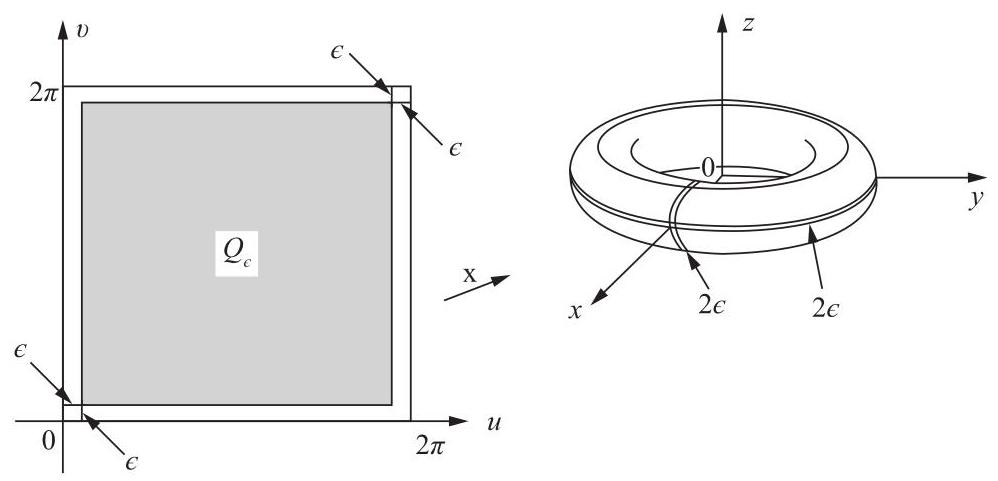
\includegraphics[max width=0.9\textwidth]{images/bo_d4b9jf3ef24c73e0334g_112_285_1555_998_481_0.jpg}
\end{center}
\hspace*{3em} 

图 2-29

这与通过初等微积分找到的值一致，例如，使用帕普斯定理计算旋转曲面的面积(参见练习 11).

\exerciseline

1. 计算以下参数化曲面在正则情况下的第一基本形式:

a. \(\mathbf{x}\left( {u,v}\right)  = \left( {a\sin u\cos v,b\sin u\sin v,c\cos u}\right)\) ；椭球面.

b. \(\mathbf{x}\left( {u,v}\right)  = \left( {{au}\cos v,{bu}\sin v,{u}^{2}}\right)\) ；椭圆抛物面.

c. \(\mathbf{x}\left( {u,v}\right)  = \left( {{au}\cosh v,{bu}\sinh v,{u}^{2}}\right)\) ；双曲抛物面.

d. \(\mathbf{x}\left( {u,v}\right)  = \left( {a\sinh u\cos v,b\sinh u\sin v,c\cosh u}\right)\) ；两叶双曲面.

2. 令 \(\mathbf{x}\left( {\varphi ,\theta }\right)  = \left( {\sin \theta \cos \varphi ,\sin \theta \sin \varphi ,\cos \theta }\right)\) 为单位球面 \({S}^{2}\) 的一个参数化.令 \(P\) 为平面 \(x = z\operatorname{cotan}\alpha ,0 < \alpha  < \pi\) ，令 \(\beta\) 为曲线 \(P \cap  {S}^{2}\) 与半子午线 \(\varphi  = {\varphi }_{0}\) 所成的锐角.计算 \(\cos \beta\) .

3. 在立体投影给出的参数化中，求出球体的第一基本形式(参见第 2-2 节练习 16).

4. 给定参数化曲面

\[
\mathbf{x}\left( {u,v}\right)  = \left( {u\cos v,u\sin v,\log \cos v + u}\right) ,\; - \frac{\pi }{2} < v < \frac{\pi }{2},
\]

证明两条曲线 \(\mathbf{x}\left( {u,{v}_{1}}\right) ,\mathbf{x}\left( {u,{v}_{2}}\right)\) 在所有曲线 \(\mathbf{x}\left( {u\text{ , const. }}\right)\) 上确定等长的线段.

5. 证明有界区域 \(R\) 在曲面 \(z = f\left( {x,y}\right)\) 上的面积 \(A\) 为

\[
A = {\iint }_{Q}\sqrt{1 + {f}_{x}^{2} + {f}_{y}^{2}}{dxdy}
\]

其中 \(Q\) 是 \(R\) 到 \({xy}\) 平面的法向投影.

6. 证明

\[
\mathbf{x}\left( {u,v}\right)  = \left( {u\sin \alpha \cos v,u\sin \alpha \sin v,u\cos \alpha }\right)
\]

\[
0 < u < \infty ,\;0 < v < {2\pi },\;\alpha  = \text{ const., }
\]

是顶点角为 \({2\alpha }\) 的锥面的参数化.在相应的坐标邻域中，证明曲线

\[
\mathbf{x}\left( {c\exp \left( {v\sin \alpha \operatorname{cotan}\beta }\right) ,v}\right) ,\;c = \text{ const., }\beta  = \text{ const., }
\]

与锥面的生成线( \(v =\) 为常数)以恒定角度 \(\beta\) 相交.

7. 参数化 \(\mathbf{x}\left( {u,v}\right)\) 的坐标曲线构成切比雪夫网，如果由它们形成的任何四边形的对边长度相等.证明这是充要条件是

\[
\frac{\partial E}{\partial v} = \frac{\partial G}{\partial u} = 0
\]

*8. 证明，只要坐标曲线构成切比雪夫网(见练习 7)，就可以重新参数化坐标邻域，使得第一基本形式的新系数为

\[
E = 1,\;F = \cos \theta ,\;G = 1,
\]

其中 \(\theta\) 是坐标曲线的角度.

*9. 证明旋转曲面总可以参数化，使得

\[
E = E\left( v\right) ,\;F = 0,\;G = 1.
\]

10. 令 \(P = \left\{  {\left( {x,y,z}\right)  \in  {R}^{3};z = 0}\right\}\) 为 \({xy}\) 平面，令 \(\mathbf{x} : U \rightarrow  P\) 为 \(P\) 的参数化，由下式给出

\[
\mathbf{x}\left( {\rho ,\theta }\right)  = \left( {\rho \cos \theta ,\rho \sin \theta }\right) ,
\]

其中

\[
U = \left\{  {\left( {\rho ,\theta }\right)  \in  {R}^{2};\rho  > 0,0 < \theta  < {2\pi }}\right\}  .
\]

计算 \(P\) 在此参数化下的第一基本形式的系数.

11. 令 \(S\) 为旋转曲面， \(C\) 为其生成曲线(参见第 2-3 节示例 4).令 \(s\) 为 \(C\) 的弧长，并用 \(\rho  = \rho \left( s\right)\) 表示 \(C\) 上对应于 \(s\) 的点的到旋转轴的距离.

a. (帕普斯定理.) 证明 \(S\) 的面积为

\[
{2\pi }{\int }_{0}^{l}\rho \left( s\right) {ds}
\]

其中 \(l\) 是 \(C\) 的长度.

b. 应用 a 部分计算旋转曲面环面的面积.

12. 证明半径为 \(r\) 的规则管绕曲线 \(\alpha\) (参见练习 10, 第 2-4 节) 的面积是 \(\alpha\) 长度的 \({2\pi r}\) 倍.

13. (广义螺旋面.) 通过以下方式获得旋转曲面和螺旋面的自然推广.设一条不与平面中的轴 \(E\) 相交的规则平面曲线 \(C\) 绕 \(E\) 进行刚性螺旋运动而移动，即，使得 \(C\) 的每一点都描述一个以 \(E\) 为轴的螺旋线(或圆).由 \(C\) 的移动生成的集合 \(S\) 称为以 \(E\) 为轴、以 \(C\) 为生成元的广义螺旋面.如果螺旋运动是绕 \(E,S\) 的纯旋转，则为旋转曲面；如果 \(C\) 是垂直于 \(E,S\) 的直线，则为(一部分)标准螺旋面(参见示例 3).

选择坐标轴，使得 \(E\) 为 \(z\) 轴，并且 \(C\) 位于 \({yz}\) 平面内.证明

a. 如果 \(\left( {f\left( s\right) ,g\left( s\right) }\right)\) 是以弧长 \(s,a < s < b\) 为参数的 \(C\) 的参数化， \(f\left( s\right)  > 0\) ，则 \(\mathbf{x} : U \rightarrow  S\) ，其中

\[
U = \left\{  {\left( {s,u}\right)  \in  {R}^{2};a < s < b,0 < u < {2\pi }}\right\}
\]

和

\[
\mathbf{x}\left( {s,u}\right)  = \left( {f\left( s\right) \cos u,f\left( s\right) \sin u,g\left( s\right)  + {cu}}\right) ,\;c = \text{ const. },
\]

是 \(S\) 的参数化.由此得出 \(S\) 是一个规则曲面.

b. 上述参数化的坐标线是正交的(即， \(F = 0\) )，当且仅当 \(\mathbf{x}\left( U\right)\) 是旋转曲面或(一部分)标准螺旋面.

14. (曲面上的梯度.) 可微函数 \(f : S \rightarrow  R\) 的梯度是一个可微映射 grad \(f : S \rightarrow  {R}^{3}\) ，它将每一点 \(p \in  S\) 映射到一个向量 grad \(f\left( p\right)  \in  {T}_{p}\left( S\right)  \subset  {R}^{3}\) ，使得

\[
\langle \operatorname{grad}f\left( p\right) ,v{\rangle }_{p} = d{f}_{p}\left( v\right) \;\text{ for all }v \in  {T}_{p}\left( S\right) .
\]

证明

a. 如果 \(E,F,G\) 是参数化 \(\mathbf{x} : U \subset  {R}^{2} \rightarrow  S\) 的第一基本形式的系数，则 \(\mathbf{x}\left( U\right)\) 上的 grad \(f\) 由下式给出

\[
\operatorname{grad}f = \frac{{f}_{u}G - {f}_{v}F}{{EG} - {F}^{2}}{\mathbf{x}}_{u} + \frac{{f}_{v}E - {f}_{u}F}{{EG} - {F}^{2}}{\mathbf{x}}_{v}.
\]

特别地，如果 \(S = {R}^{2}\) 具有坐标 \(x,y\) ，

\[
\operatorname{grad}f = {f}_{x}{e}_{1} + {f}_{y}{e}_{2},
\]

其中 \(\left\{  {{e}_{1},{e}_{2}}\right\}\) 是 \({R}_{2}\) 的正则基(因此，定义与平面中梯度的通常定义一致).

b. 如果固定 \(p \in  S\) 并让 \(v\) 在 \({T}_{p}\left( s\right)\) 中的单位圆 \(\left| v\right|  = 1\) 中变化，则 \(d{f}_{p}\left( v\right)\) 最大当且仅当 \(v = \operatorname{grad}f/\left| {\operatorname{grad}f}\right|\) (因此，grad \(f\left( p\right)\) 给出了 f 在 \(p\) 处最大变化的方向).

c. 如果在水平曲线 \(C = \{ q \in  S;f\left( q\right)  =\) const. 的所有点上，梯度 \(f \neq  0\) 存在，则 \(C\) 是 \(S\) 上的正则曲线，并且梯度 \(f\) 在 \(C\) 的所有点上都垂直于 \(C\) .

\section*{15. (曲线的直交族.)}

a. 设 \(E,F,G\) 是正则曲面 \(S\) 在参数化 \(\mathbf{x} : U \subset  {R}^{2} \rightarrow  S\) 下的第一基本形式的系数.设 \(\varphi \left( {u,v}\right)  =\) const. 和 \(\psi \left( {u,v}\right)  =\) const. 是 \(\mathbf{x}\left( U\right)  \subset  S\) 上的两条正则曲线族(参见习题 28，第 2-4 节).证明这两条曲线族是直交的(即，当不同族的两条曲线相交时，它们的切线是直交的)当且仅当

\[
E{\varphi }_{v}{\psi }_{v} - F\left( {{\varphi }_{u}{\psi }_{v} + {\varphi }_{v}{\psi }_{u}}\right)  + G{\varphi }_{u}{\psi }_{u} = 0.
\]

b. 应用 a 部分证明，在螺旋面(例 3)的坐标邻域 \(\mathbf{x}\left( U\right)\) 上，两条正则曲线族

\[
v\cos u = \text{ const., }\;v \neq  0,
\]

\[
\left( {{v}^{2} + {a}^{2}}\right) {\sin }^{2}u = \text{ const., }\;v \neq  0,\;u \neq  \pi ,
\]

是直交的.

\section*{2-6. 曲面的定向†}

在本节中，我们将讨论曲面可以在何种意义下以及何时可以被定向.直观地说，由于正则曲面 \(S\) 的每一点 \(p\) 都有一个切平面 \({T}_{p}\left( S\right)\) ，选择 \({T}_{p}\left( S\right)\) 的一个定向会在 \(p\) 的邻域中诱导一个定向，即，关于邻域中每一点的足够小的闭合曲线的正向运动的概念(图 2-30).如果可以为每个 \(p \in  S\) 做出这个选择，使得在任何两个邻域的交集中定向一致，则称 \(S\) 是可定向的.如果不可能，则称 \(S\) 是不可定向的.

现在我们将使这些想法精确化.通过固定正则曲面 \(S\) 上一点 \(p\) 的邻域的参数化 \(\mathbf{x}\left( {u,v}\right)\) ，我们确定了切平面 \({T}_{p}\left( S\right)\) 的一个定向，即，相关有序基 \(\left\{  {{\mathbf{x}}_{u},{\mathbf{x}}_{v}}\right\}\) 的定向.如果 \(p\) 属于另一个参数化 \(\overline{\mathbf{x}}\left( {\bar{u},\bar{v}}\right)\) 的坐标邻域，则新基 \(\left\{  {{\overline{\mathbf{x}}}_{\bar{u}},{\overline{\mathbf{x}}}_{\bar{v}}}\right\}\) 用第一个基表示为

\[
{\overline{\mathbf{x}}}_{\bar{u}} = {\mathbf{x}}_{u}\frac{\partial u}{\partial \bar{u}} + {\mathbf{x}}_{v}\frac{\partial v}{\partial \bar{u}},
\]

\[
{\mathbf{x}}_{\bar{v}} = {\mathbf{x}}_{u}\frac{\partial u}{\partial \bar{v}} + {\mathbf{x}}_{v}\frac{\partial v}{\partial \bar{v}}
\]

其中 \(u = u\left( {\bar{u},\bar{v}}\right)\) 和 \(v = v\left( {\bar{u},\bar{v}}\right)\) 是坐标变换的表达式.因此，基 \(\left\{  {{\mathbf{x}}_{u},{\mathbf{x}}_{v}}\right\}\) 和 \(\left\{  {{\overline{\mathbf{x}}}_{\bar{u}},{\overline{\mathbf{x}}}_{\bar{v}}}\right\}\) 确定相同的 \({T}_{p}\left( S\right)\) 定向当且仅当雅可比行列式

\[
\frac{\partial \left( {u,v}\right) }{\partial \left( {\bar{u},\bar{v}}\right) }
\]

的坐标变换是正的.



†本节在初读时可以省略.



\begin{center}
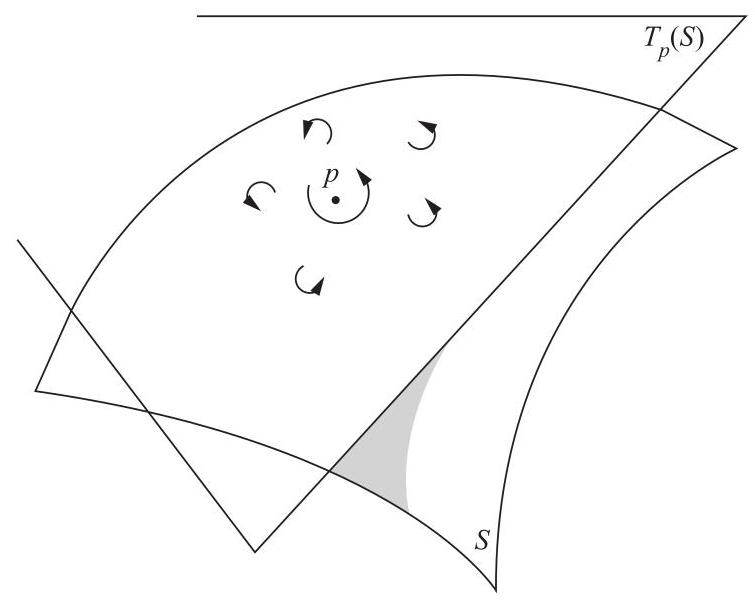
\includegraphics[max width=0.6\textwidth]{images/bo_d4b9jf3ef24c73e0334g_117_381_191_755_602_0.jpg}
\end{center}
\hspace*{3em} 

图 2-30

定义 1. 正则曲面 \(S\) 称为可定向的，如果可以用一组坐标邻域覆盖它，使得如果一点 \(\mathrm{p} \in  S\) 属于该族中的两个邻域，则坐标变换在 p 点处具有正的雅可比行列式.这种族的选择称为 \(S\) 的一个定向，在这种情况下， \(S\) 称为定向的.如果不可能做出这种选择，则该曲面称为不可定向的.

示例 1. 可微函数(参见第 2-2 节，命题 1)的图像曲面是可定向曲面.事实上，所有能被一个坐标邻域覆盖的曲面都是平凡可定向的.

示例 2. 球面是可定向曲面.我们不进行直接计算，而是采用一般论证.球面可以用两个坐标邻域覆盖(使用立体投影；参见第 2-2 节的练习 16)，参数为 \(\left( {u,v}\right)\) 和 \(\left( {\bar{u},\bar{v}}\right)\) ，使得这两个邻域的交集 \(W\) (球面除去两个点)是一个连通集.在 \(W\) 中固定一点 \(p\) .如果在 \(p\) 处的坐标变换的雅可比行列式为负，我们就交换第一个系统中的 \(u\) 和 \(v\) ，此时雅可比行列式变为正.由于在 \(W\) 中雅可比行列式不为零，且在 \(p \in  W\) 处为正，因此根据 \(W\) 的连通性可知，雅可比行列式处处为正.因此，存在一个满足定义 1 的坐标邻域族，所以球面是可定向的.

根据刚才的论证，可以清楚地看出，如果一个正则曲面可以被两个坐标邻域覆盖，且它们的交集是连通的，那么这个曲面就是可定向的.

在给出非定向曲面的例子之前，我们将对 \({R}^{3}\) 中正则曲面可定向性的概念给出一个几何解释.

正如我们在第 2-4 节中看到的，给定 \(p\) 处的一组坐标 \(\mathbf{x}\left( {u,v}\right)\) ，我们根据以下规则在 \(p\) 处有一个确定的单位法向量 \(N\) 的选择:

\[
N = \frac{{\mathbf{x}}_{u} \land  {\mathbf{x}}_{v}}{\left| {\mathbf{x}}_{u} \land  {\mathbf{x}}_{v}\right| }\left( p\right) . \tag{1}
\]

取 \(p\) 处的另一组局部坐标 \(\overline{\mathbf{x}}\left( {\bar{u},\bar{v}}\right)\) ，我们看到:

\[
{\overline{\mathbf{x}}}_{\bar{u}} \land  {\overline{\mathbf{x}}}_{\bar{v}} = \left( {{\mathbf{x}}_{u} \land  {\mathbf{x}}_{v}}\right) \frac{\partial \left( {u,v}\right) }{\partial \left( {\bar{u},\bar{v}}\right) }, \tag{2}
\]

其中 \(\partial \left( {u,v}\right) /\partial \left( {\bar{u},\bar{v}}\right)\) 是坐标变换的雅可比行列式.因此， \(N\) 将保持其符号或改变其符号，取决于 \(\partial \left( {u,v}\right) /\partial \left( {\bar{u},\bar{v}}\right)\) 分别是正还是负.

通过一个在开集 \(U \subset  S\) 上的可微单位法向量场，我们将指一个可微映射 \(N : U \rightarrow  {R}^{3}\) ，它将每个 \(q \in  U\) 与 \(S\) 在 \(q\) 处的单位法向量 \(N\left( q\right)  \in  {R}^{3}\) 相关联.

命题 1. 正则曲面 \(S \subset  {\mathbb{R}}^{3}\) 是可定向的，当且仅当在 \(S\) 上存在一个可微单位法向量场 \(N : S \rightarrow  {\mathbb{R}}^{3}\) .

证明.如果 \(S\) 是可定向的，那么可以用一组坐标邻域覆盖它，使得在其中任意两个邻域的交集中，坐标变换具有正的雅可比行列式.在每个邻域的点 \(p = \mathbf{x}\left( {u,v}\right)\) 处，我们通过公式 (1) 定义 \(N\left( p\right)  = N\left( {u,v}\right)\) . \(N\left( p\right)\) 是良定义的，因为如果 \(p\) 属于两个坐标邻域，参数分别为 \(\left( {u,v}\right)\) 和 \(\left( {\bar{u},\bar{v}}\right)\) ，则根据公式 (2)，法向量 \(N\left( {u,v}\right)\) 和 \(N\left( {\bar{u},\bar{v}}\right)\) 重合.此外，根据公式 (1)， \(N\left( {u,v}\right)\) 在 \({R}^{3}\) 中的坐标是 \(\left( {u,v}\right)\) 的可微函数，因此映射 \(N : S \rightarrow  {R}^{3}\) 是可微的，正如所期望的那样.

另一方面，设 \(N : S \rightarrow  {R}^{3}\) 为一个可微的单位法向量场，并考虑一个覆盖 \(S\) 的连通坐标邻域族.对于每个坐标邻域 \(\mathbf{x}\left( U\right) ,U \subset  {R}^{2}\) 中的点 \(p = \mathbf{x}\left( {u,v}\right)\) ，通过 \(N\) 的连续性，并在必要时交换 \(u\) 和 \(v\) ，可以安排使得

\[
N\left( p\right)  = \frac{{\mathbf{x}}_{u} \land  {\mathbf{x}}_{v}}{\left| {\mathbf{x}}_{u} \land  {\mathbf{x}}_{v}\right| }.
\]

事实上，内积

\[
\left\langle  {N\left( p\right) ,\frac{{\mathbf{x}}_{u} \land  {\mathbf{x}}_{v}}{\left| {\mathbf{x}}_{u} \land  {\mathbf{x}}_{v}\right| }}\right\rangle   = f\left( p\right)  =  \pm  1
\]

是 \(\mathbf{x}\left( U\right)\) 上的连续函数.由于 \(\mathbf{x}\left( U\right)\) 是连通的， \(f\) 的符号是常数.如果 \(f =  - 1\) ，我们在参数化中交换 \(u\) 和 \(v\) ，则命题成立.

以此方式处理所有坐标邻域，我们得到，在其中任意两个邻域的交集中，例如 \(\mathbf{x}\left( {u,v}\right)\) 和 \(\overline{\mathbf{x}}\left( {\bar{u},\bar{v}}\right)\) ，雅可比行列式

\[
\frac{\partial \left( {u,v}\right) }{\partial \left( {\bar{u},\bar{v}}\right) }
\]

必定为正；否则，我们将得到

\[
\frac{{\mathbf{x}}_{u} \land  {\mathbf{x}}_{v}}{\left| {\mathbf{x}}_{u} \land  {\mathbf{x}}_{v}\right| } = N\left( p\right)  =  - \frac{{\bar{\mathbf{x}}}_{\bar{u}} \land  {\bar{\mathbf{x}}}_{\bar{v}}}{\left| {\bar{\mathbf{x}}}_{\bar{u}} \land  {\bar{\mathbf{x}}}_{\bar{v}}\right| } =  - N\left( p\right) ,
\]

这是一个矛盾.因此，经过 \(u\) 和 \(v\) 的某些交换后，给定的坐标邻域族满足定义 1 的条件，因此 \(S\) 是可定向的.Q.E.D.

注.正如证明所示，为了使 \(S\) 可定向，我们只需要要求存在一个连续的单位向量场在 \(S\) 上.这样的向量场将自动是可微的.

例 3.现在我们将描述一个不可定向曲面的例子，即所谓的莫比乌斯带.该曲面是通过考虑由 \({x}^{2} + {y}^{2} = 4\) 给出的圆 \({S}^{1}\) 和由 \({yz}\) 平面中的 \(y = 2,\left| z\right|  < 1\) 给出的开线段 \({AB}\) 得到的(见图 2-31).我们移动 \({AB}\) 的中心 \(C\) 沿着 \({S}^{1}\) ，并在 \({Cz}\) 平面中绕 \(C\) 旋转 \({AB}\) ，使得当 \(C\) 经过角度 \(u,{AB}\) 时， \({AB}\) 旋转了角度 \(u/2\) .当 \(c\) 完成绕圆一周的行程时， \({AB}\) 返回其初始位置，其端点被反转.

\begin{center}
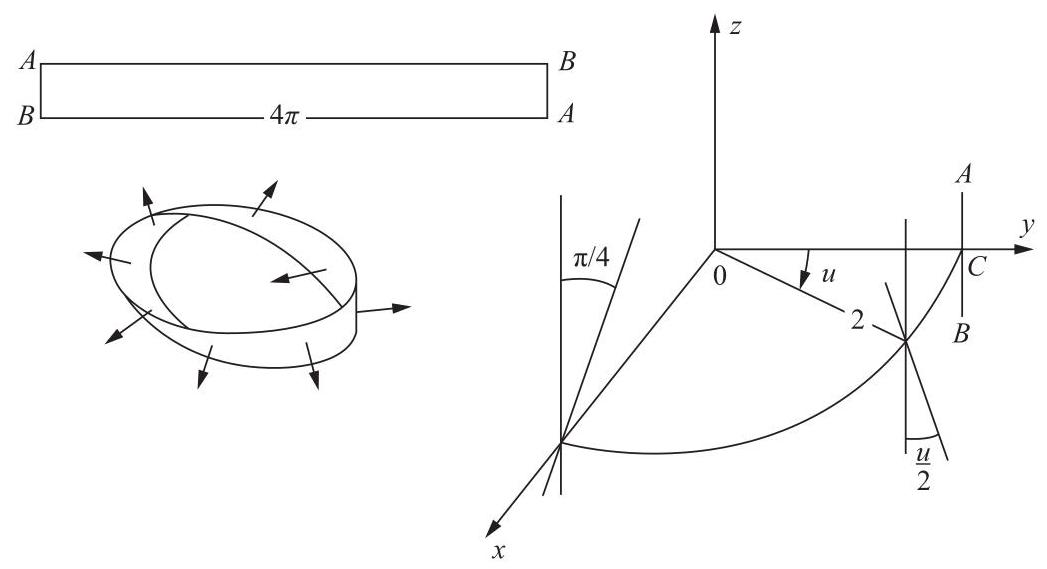
\includegraphics[max width=0.9\textwidth]{images/bo_d4b9jf3ef24c73e0334g_119_242_1470_1047_569_0.jpg}
\end{center}
\hspace*{3em} 

图 2-31

从可微性的角度来看，这就像我们识别了一个矩形的相对(垂直)边，给矩形一个扭曲，使得边 \({AB}\) 的每个点都与其对称点识别(图 2-31).

从几何上看，莫比乌斯带 \(M\) 是一个正则的、不可定向的曲面.事实上，如果 \(M\) 是可定向的，就会存在一个可微的单位法向量场 \(N : M \rightarrow  {R}^{3}\) .沿着圆 \({x}^{2} + {y}^{2} = 4\) 取这些向量，我们看到在完成一周行程后，向量 \(N\) 返回其原始位置，如 \(- N\) ，这是一个矛盾.

现在我们将给出上述事实的解析证明.

莫比乌斯带的坐标系 \(\mathbf{x} : U \rightarrow  M\) 由下式给出

\[
\mathbf{x}\left( {u,v}\right)  = \left( {\left( {2 - v\sin \frac{u}{2}}\right) \sin u,\left( {2 - v\sin \frac{u}{2}}\right) \cos u,v\cos \frac{u}{2}}\right) ,
\]

其中 \(0 < u < {2\pi }\) 和 \(- 1 < v < 1\) .相应的坐标邻域省略了开区间 \(u = 0\) 的点.然后，通过将 \(u\) 的原点置于 \(x\) 轴上，我们得到另一个参数化 \(\overline{\mathbf{x}}\left( {\bar{u},\bar{v}}\right)\) ，由下式给出

\[
x = \left\{  {2 - \bar{v}\sin \left( {\frac{\pi }{4} + \frac{\bar{u}}{2}}\right) }\right\}  \cos \bar{u},
\]

\[
y =  - \left\{  {2 - \bar{v}\sin \left( {\frac{\pi }{4} + \frac{\bar{u}}{2}}\right) }\right\}  \sin \bar{u},
\]

\[
z = \bar{v}\cos \left( {\frac{\pi }{4} + \frac{\bar{u}}{2}}\right) ,
\]

其坐标邻域省略了区间 \(u = \pi /2\) .这两个坐标邻域覆盖了莫比乌斯带，并可用于证明它是一个正则曲面.

请注意，两个坐标邻域的交集不是连通的，而是由两个连通分量组成:

\[
{W}_{1} = \left\{  {\mathbf{x}\left( {u,v}\right)  : \frac{\pi }{2} < u < {2\pi }}\right\}  ,
\]

\[
{W}_{2} = \left\{  {\mathbf{x}\left( {u,v}\right)  : 0 < u < \frac{\pi }{2}}\right\}
\]

坐标变换由以下给出

\[
\left. \begin{array}{l} \bar{u} = u - \frac{\pi }{2} \\  \bar{v} = v \end{array}\right\}  \;\text{ in }{W}_{1},
\]

和

\[
\left. \begin{array}{l} \bar{u} = \frac{3\pi }{2} + u \\  \bar{v} =  - v \end{array}\right\}  \;\text{ in }{W}_{2}.
\]

由此可知

\[
\frac{\partial \left( {\bar{u},\bar{v}}\right) }{\partial \left( {u,v}\right) } = 1 > 0\;\text{ in }{W}_{1}
\]

并且

\[
\frac{\partial \left( {\bar{u},\bar{v}}\right) }{\partial \left( {u,v}\right) } =  - 1 < 0\;\text{ in }{W}_{2}.
\]

为了证明莫比乌斯带是不可定向的，我们假设可以定义一个单位法向量的可微场 \(N : M \rightarrow  {R}^{3}\) .如果需要，交换 \(u\) 和 \(v\) ，我们可以假设

\[
N\left( p\right)  = \frac{{\mathbf{x}}_{u} \land  {\mathbf{x}}_{v}}{\left| {\mathbf{x}}_{u} \land  {\mathbf{x}}_{v}\right| }
\]

对于 \(\mathbf{x}\left( {u,v}\right)\) 的坐标邻域中的任何 \(p\) .类似地，我们可以假设

\[
N\left( p\right)  = \frac{{\bar{\mathbf{x}}}_{\bar{u}} \land  {\bar{\mathbf{x}}}_{\bar{v}}}{\left| {\bar{\mathbf{x}}}_{\bar{u}} \land  {\bar{\mathbf{x}}}_{\bar{v}}\right| }
\]

在 \(\overline{\mathbf{x}}\left( {\bar{u},\bar{v}}\right)\) 的坐标邻域的所有点上.然而，坐标变换的雅可比行列式在 \({W}_{1}\) 或 \({W}_{2}\) 中必须是 -1(取决于需要进行哪种类型的 \(u \rightarrow  v,\bar{u} \rightarrow  \bar{v}\) 变换).如果 \(p\) 是该交集分量上的一个点，那么 \(N\left( p\right)  =  - N\left( p\right)\) ，这是一个矛盾.

我们已经看到，可微函数的图像曲面是可定向的.现在我们将证明可微函数的正则值逆像曲面也是可定向的.这是在 \({R}^{3}\) 中构造不可定向正则曲例相对困难的原因之一.

命题 2. 如果一个正则曲面由 \(S = \left\{  {\left( {x,\mathrm{y},\mathrm{z}}\right)  \in  {\mathbb{R}}^{3}}\right.\) ； \(\mathrm{f}\left( {x,\mathrm{y},\mathrm{z}}\right)  = \mathrm{a}\}\) 给出，其中 \(\mathrm{f} : \mathrm{U} \subset  {\mathbb{R}}^{3} \rightarrow  \mathbb{R}\) 是可微的，a 是 \(\mathrm{f}\) 的一个正则值，那么 \(S\) 是可定向的.

证明.给定一个点 \(\left( {{x}_{0},{y}_{0},{z}_{0}}\right)  = p \in  S\) ，考虑曲面 \(S\) 上通过 \(p\) 在 \(t = {t}_{0}\) 处的参数化曲线 \(\left( {x\left( t\right) ,y\left( t\right) ,z\left( t\right) }\right) ,t \in  I\) .

\[
f\left( {x\left( t\right) ,y\left( t\right) ,z\left( t\right) }\right)  = a
\]

对于所有 \(t \in  I\) .通过对该表达式两边关于 \(t\) 求导，我们在 \(t = {t}_{0}\) 处得到

\[
{f}_{x}\left( p\right) {\left( \frac{dx}{dt}\right) }_{{t}_{0}} + {f}_{y}\left( p\right) {\left( \frac{dy}{dt}\right) }_{{t}_{0}} + {f}_{z}\left( p\right) {\left( \frac{dz}{dt}\right) }_{{t}_{0}} = 0.
\]

这表明曲线在 \(t = {t}_{0}\) 处的切向量垂直于 \(p\) 处的向量 \(\left( {{f}_{x},{f}_{y},{f}_{z}}\right)\) .由于曲线和点是任意的，我们得出结论

\[
N\left( {x,y,z}\right)  = \left( {\frac{{f}_{x}}{\sqrt{{f}_{x}^{2} + {f}_{y}^{2} + {f}_{z}^{2}}},\frac{{f}_{y}}{\sqrt{{f}_{x}^{2} + {f}_{y}^{2} + {f}_{z}^{2}}},\frac{{f}_{z}}{\sqrt{{f}_{x}^{2} + {f}_{y}^{2} + {f}_{z}^{2}}}}\right)
\]

是 \(S\) 上的一个单位法向量的可微场.结合命题 1，这表明 \(S\) 如期望的那样是可定向的.Q.E.D.

最后的说明.定向绝对不是正则曲面的局部性质.局部上，每个正则曲面都同胚于平面上的一个开集，因此是可定向的.定向是一个全局性质，因为它涉及到整个曲面.我们将在本书后面(第 5 章)讨论更多关于全局性质的内容.

\exerciseline

1. 设 \(S\) 是一个由坐标邻域 \({V}_{1}\) 和 \({V}_{2}\) 覆盖的正则曲面.假设 \({V}_{1} \cap  {V}_{2}\) 有两个连通分量 \({W}_{1},{W}_{2}\) ，并且坐标变换的雅可比行列式在 \({W}_{1}\) 中为正，在 \({W}_{2}\) 中为负.证明 \(S\) 是不可定向的.

2. 令 \({S}_{2}\) 为一个可定向正则曲面，令 \(\varphi  : {S}_{1} \rightarrow  {S}_{2}\) 为一个可微映射，该映射在每一点 \(p \in  {S}_{1}\) 处都是局部微分同胚.证明 \({S}_{1}\) 是可定向的.

3. 莫比乌斯带的面积概念是否可以赋予意义？如果可以，请建立一个积分来计算它.

4. 令 \(S\) 为一个可定向曲面，令 \(\left\{  {U}_{\alpha }\right\}\) 和 \(\left\{  {V}_{\beta }\right\}\) 为覆盖 \(S\) 的两个坐标邻域族(即 \(\bigcup {U}_{\alpha } = S = \bigcup {V}_{\beta }\) )，并满足定义 1 的条件(即，在每个族中，坐标变换具有正雅可比行列式).我们说 \(\left\{  {U}_{\alpha }\right\}\) 和 \(\left\{  {V}_{\beta }\right\}\) 确定了 \(S\) 的相同定向，如果这两个族的并集再次满足定义 1 的条件.

证明一个正则、连通、可定向的曲面只有两种不同的定向.

5. 令 \(\varphi  : {S}_{1} \rightarrow  {S}_{2}\) 为一个微分同胚.

a. 证明 \({S}_{1}\) 是可定向的当且仅当 \({S}_{2}\) 是可定向的(因此，可定向性由微分同胚保持).

b. 令 \({S}_{1}\) 和 \({S}_{2}\) 为可定向且已定向的.证明微分同胚 \(\varphi\) 在 \({S}_{2}\) 中诱导一个定向.使用球面的对径映射(练习 1，第 2-3 节)来表明这个定向可能与初始定向不同(参见练习 4)(因此，定向本身可能不被微分同胚保持；但请注意，如果 \({S}_{1}\) 和 \({S}_{2}\) 是连通的，微分同胚要么保持定向，要么“反转”定向).

6. 定义正则曲线 \(C \subset  {R}^{3}\) 的定向概念，并证明如果 \(C\) 是连通的，则最多存在两种不同的定向(根据练习 4 的意义)(实际上存在两种，但这更难证明).

7. 证明如果一个正则曲面 \(S\) 包含一个与莫比乌斯带微分同胚的开集，那么 \(S\) 是不可定向的.

\section*{2-7. 紧致可定向曲面的刻画 \({}^{ \dagger  }\)}

命题 2-6.2 的逆命题，即一个可定向曲面在 \({\mathbb{R}}^{3}\) 中是某个可微函数正则值f的原像，是成立的，但证明 nontrivial.即使在紧致曲面(本节定义)的特殊情况下，证明也很有启发性，并提供了微分几何中一个全局定理的有趣例子.本节将完全致力于证明这个逆命题.

设 \(S \subset  {R}^{3}\) 是一个可定向曲面.证明的关键在于表明，我们可以在通过 \(p \in  S\) 的法线上选择一个围绕 \(p\) 的长度为，比如说， \(2{\epsilon }_{p}\left( {\epsilon }_{p}\right.\) 的开区间 \({I}_{p}\) ，这个长度随 \(\left. p\right)\) 而变化，使得如果 \(p \neq  q \in  S\) ，那么 \({I}_{p} \cap  {I}_{q} = \phi\) .因此，并集 \(\bigcup {I}_{p},p \in  S\) ，构成 \({R}^{3}\) 的一个开集 \(V\) ，它包含 \(S\) 并具有这样的性质:通过 \(V\) 的每一点都有一条唯一的法线到 \(S;V\) ，然后称为 \(S\) 的管状邻域(图 2-32).

\begin{center}
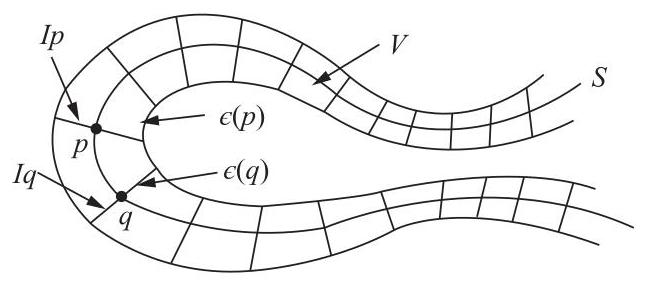
\includegraphics[max width=0.5\textwidth]{images/bo_d4b9jf3ef24c73e0334g_123_180_1402_646_286_0.jpg}
\end{center}
\hspace*{3em} 

图 2-32. 管状邻域.

暂时假设存在一个可定向曲面 \(S\) 的管状邻域 \(V\) .然后我们可以如下定义一个函数 \(g : V \rightarrow  R\) :固定 \(S\) 的一个定向.注意到管状邻域 \(V\) 的两个线段 \({I}_{P}\) 和 \({I}_{q}\) ， \(p \neq  q\) ，不相交.因此，通过每一点 \(P \in  V\) 都有一条唯一的法线到 \(S\) ，它在 \(S\) 上相交于一点 \(p\) ；根据定义， \(g\left( P\right)\) 是从 \(p\) 到 \(P\) 的距离，其符号由 \(p\) 处单位法向量的方向给出.如果我们能证明 \(g\) 是一个可微函数，并且 0 是 \(g\) 的一个正则值，那么我们将得到 \(S = {g}^{-1}\left( 0\right)\) ，正如我们希望证明的那样.



†本节在初读时可以省略.



现在我们将开始证明可定向曲面管状邻域的存在性.我们首先证明这个事实的一个局部版本；也就是说，我们将证明对于正则曲面的每一点 \(p\) ，都存在一个具有管状邻域的邻域.

命题 1. 设 \(S\) 是一个正则曲面， \(\mathbf{x} : \mathrm{U} \rightarrow  S\) 是点 \(\mathrm{p} = \mathbf{x}\left( {{\mathrm{u}}_{0},{\mathrm{v}}_{0}}\right)  \in  S\) 的一个邻域的参数化.那么存在 \(S\) 中 \(\mathrm{p}\) 的一个邻域 \(\mathrm{W} \subset  \mathbf{x}\left( \mathrm{U}\right)\) 和一个数 \(\epsilon  > 0\) ，使得通过点 \(\mathrm{q} \in  \mathrm{W}\) 的法线段，以 \(\mathrm{q}\) 为中心，长度为 \({2\epsilon }\) ，是互不相交的(也就是说， \(\mathrm{W}\) 有一个管状邻域).

证明.考虑映射 \(\mathrm{F} : \mathrm{U} \times  \mathbb{R} \rightarrow  {\mathbb{R}}^{3}\) ，由下式给出

\[
F\left( {u,v;t}\right)  = \mathbf{x}\left( {u,v}\right)  + {tN}\left( {u,v}\right) ,\;\left( {u,v}\right)  \in  U,\;t \in  R,
\]

其中 \(N\left( {u,v}\right)  = \left( {{N}_{x},{N}_{y},{N}_{z}}\right)\) 是单位法向量在

\[
\mathbf{x}\left( {u,v}\right)  = \left( {x\left( {u,v}\right) ,y\left( {u,v}\right) ,z\left( {u,v}\right) }\right) .
\]

从几何上看， \(F\) 将“圆柱体” \(U \times  R\) 中的点 \(\left( {u,v;t}\right)\) 映射到法线 \(S\) 上距离 \(\mathbf{x}\left( {u,v}\right) .F\)  \(t\) 的点，该映射是可微的，其在 \(t = 0\) 处的雅可比矩阵为

\[
\left| \begin{array}{lll} \frac{\partial x}{\partial u} & \frac{\partial y}{\partial u} & \frac{\partial z}{\partial u} \\  \frac{\partial x}{\partial v} & \frac{\partial y}{\partial v} & \frac{\partial z}{\partial v} \\  {N}_{x} & {N}_{y} & {N}_{z} \end{array}\right|  = \left| {{\mathbf{x}}_{u} \land  {\mathbf{x}}_{v}}\right|  \neq  0.
\]

根据反函数定理，在 \(U \times  R\) 中存在一个平行六面体，例如

\[
{u}_{0} - \delta  < u < {u}_{0} + \delta ,\;{v}_{0} - \delta  < v < {v}_{0} + \delta ,\; - \epsilon  < t < \epsilon ,
\]

在此限制下， \(F\) 是一一映射.但这表示在 \(F\) 将矩形 \(W\) 的像中

\[
{u}_{0} - \delta  < u < {u}_{0} + \delta ,\;{v}_{0} - \delta  < v < {v}_{0} + \delta
\]

具有中心 \(q \in  W\) 且长度为 \(< {2\epsilon }\) 的法线段不相交.Q.E.D.

此时，观察以下几点很方便.函数 \(g : V \rightarrow  R\) (通过假设管状邻域 \(V\) 的存在而定义)是可微的，并且具有 0 作为正则值，这是一个局部事实，可以立即证明.

命题 2. 假设存在一个可定向曲面 \(S \subset  {\mathbb{R}}^{3}\) 的管状邻域 \(\mathrm{V} \subset  {\mathbb{R}}^{3}\) ，并为 \(S\) 选择一个定向.那么函数 \(\mathrm{g} : \mathrm{V} \rightarrow  \mathbb{R}\) 是可微的，并且具有零作为正则值.该函数定义为从 \(\mathrm{V}\) 中的一点到通过该点的唯一法线的垂足的定向距离.

证明. 让我们再次审视命题 1 中定义的映射 \(F : U \times  R \rightarrow  {R}^{3}\) ，现在我们假设参数化 \(\mathbf{x}\) 与给定的定向兼容.用 \(x,y,z\) 表示 \(F\left( {u,v,t}\right)  = \mathbf{x}\left( {u,v}\right)  + \; {tN}\left( {u,v}\right)\) 的坐标，我们可以写出

\[
F\left( {u,v,t}\right)  = \left( {x\left( {u,v,t}\right) ,y\left( {u,v,t}\right) ,z\left( {u,v,t}\right) }\right) .
\]

由于雅可比矩阵 \(\partial \left( {x,y,z}\right) /\partial \left( {u,v,t}\right)\) 在 \(t = 0\) 处不为零，我们可以在某个平行六面体 \(Q\) 中反转 \(F\) ，

\[
{u}_{0} - \delta  < u < {u}_{0} + \delta ,\;{v}_{0} - \delta  < v < {v}_{0} + \delta ,\; - \epsilon  < t < \epsilon ,
\]

得到一个可微映射

\[
{F}^{-1}\left( {x,y,z}\right)  = \left( {u\left( {x,y,z}\right) ,v\left( {x,y,z}\right) ,t\left( {x,y,z}\right) }\right) ,
\]

其中 \(\left( {x,y,z}\right)  \in  F\left( Q\right)  \subset  V\) .但是，命题 2 陈述中的函数 \(g : V \rightarrow  R\) 限制在 \(F\left( Q\right)\) 上正是 \(t = t\left( {x,y,z}\right)\) .因此， \(g\) 是可微的.此外，0 是 \(t\) 的正则值；否则

\[
\frac{\partial t}{\partial x} = \frac{\partial t}{\partial y} = \frac{\partial t}{\partial z} = 0
\]

在某个点 \(t = 0\) 处；因此，微分 \(d{F}^{-1}\) 对于 \(t = 0\) 将是奇异的，这是矛盾的.Q.E.D.

为了从局部过渡到全局，即证明整个可定向曲面的管状邻域的存在性，我们需要一些拓扑论证.我们将限制在紧致曲面上，我们现在将定义这些曲面.

设 \(A\) 是 \({R}^{3}\) 的一个子集.我们称 \(p \in  {R}^{3}\) 是 \(A\) 的一个极限点，如果 \({R}^{3}\) 中 \(p\) 的每个邻域都包含一个不同于 \(p.A\) 的 \(A\) 中的点.如果一个集合包含其所有的极限点，则称该集合是闭集.如果一个集合被包含在 \({R}^{3}\) 的某个球中，则称该集合是有界的.如果 \(A\) 是闭集且有界，则称其为紧集.

球面和环面是紧致曲面.旋转抛物面 \(z = {x}^{2} + {y}^{2},\left( {x,y}\right)  \in  {R}^{2}\) 是闭曲面，但由于无界，它不是紧致曲面.平面中的圆盘 \({x}^{2} + {y}^{2} < 1\) 和莫比乌斯带是有界的但不是闭合的，因此是非紧致的.

我们需要 \({R}^{3}\) 的紧致子集的一些性质，现在我们将陈述这些性质.两点 \(p,q \in  {R}^{3}\) 之间的距离将用 \(d\left( {p,q}\right)\) 表示.

性质 1 (Bolzano-Weierstrass).设 \(\mathrm{A} \subset  {\mathbb{R}}^{3}\) 为紧致集.则 \(\mathrm{A}\) 的每个无限子集在 \(\mathrm{A}\) 中至少有一个极限点.

性质 2 (Heine-Borel).设 \(\mathrm{A} \subset  {\mathbb{R}}^{3}\) 为一个紧集，设 \(\left\{  {\mathrm{U}}_{\alpha }\right\}\) 为 \(\mathrm{A}\) 的一个开集族，使得 \(\mathop{\bigcup }\limits_{\alpha }{\mathrm{U}}_{\alpha } \supset  \mathrm{A}\) .则可以选取有限个 \({\mathrm{U}}_{{k}_{1}},{\mathrm{U}}_{{k}_{2}},\ldots ,{\mathrm{U}}_{{k}_{n}}\) 个 \({\mathrm{U}}_{\alpha }\) ，使得 \(\bigcup {\mathrm{U}}_{{k}_{i}} \supset  \mathrm{A},\mathrm{i} = 1,\ldots ,N\) .

性质 3 (Lebesgue).设 \(\mathrm{A} \subset  {\mathbb{R}}^{3}\) 为紧致集， \(\left\{  {\mathrm{U}}_{\alpha }\right\}\) 为 \(\mathrm{A}\) 的一组开集族，使得 \(\mathop{\bigcup }\limits_{\alpha }{\mathrm{U}}_{\alpha } = \mathrm{A}\) .则存在一个数 \(\delta  > 0\) (该集族 \(\left. \left\{  {\mathrm{U}}_{\alpha }\right\}  \right)\) 的 Lebesgue 数)，使得当两点 \(\mathrm{p},\mathrm{q} \in  \mathrm{A}\) 的距离为 \(\mathrm{d}\left( {\mathrm{p},\mathrm{q}}\right)  < \delta\) 时， \(\mathrm{p}\) 和 \(\mathrm{q}\) 属于某个 \({\mathrm{U}}_{\alpha }\) .

性质 1 和 2 通常在高等微积分课程中证明.为完整起见，我们现在证明性质 3.本书稍后 (第 5 章附录) 将更系统地讨论 \({R}^{n}\) 中的紧致集，并给出性质 1 和 2 的证明.

性质 3 的证明.假设不存在满足陈述条件的 \(\delta  > 0\) ；也就是说，给定 \(1/n\) ，存在点 \({p}_{n}\) 和 \({q}_{n}\) 使得 \(d\left( {{p}_{n},{q}_{n}}\right)  < 1/n\) ，但 \({p}_{n}\) 和 \({q}_{n}\) 不属于族 \(\left\{  {U}_{\alpha }\right\}\) 的同一个开集.令 \(n = 1,2,\ldots\) ，我们得到两个无限点集 \(\left\{  {p}_{n}\right\}\) 和 \(\left\{  {q}_{n}\right\}\) ，根据性质 1，它们分别有极限点 \(p\) 和 \(q\) .由于 \(d\left( {{p}_{n},{q}_{n}}\right)  < 1/n\) ，我们可以选择这些极限点使得 \(p = q\) .但对于某个 \(\alpha\) ，有 \(p \in  {U}_{\alpha }\) ，因为 \(p \in  A = \mathop{\bigcup }\limits_{\alpha }{U}_{\alpha }\) ，并且由于 \({U}_{\alpha }\) 是一个开集，存在一个以 \(p\) 为中心的开球 \({B}_{\epsilon }\left( p\right)\) ，使得 \({B}_{\epsilon }\left( p\right)  \subset  {U}_{\alpha }\) .由于 \(p\) 是 \(\left\{  {p}_{n}\right\}\) 和 \(\left\{  {q}_{n}\right\}\) 的极限点，对于足够大的 \(n\) ，存在 \({B}_{\epsilon }\left( p\right)  \subset  {U}_{\alpha }\) 中的点 \({p}_{n}\) 和 \({q}_{n}\) ；也就是说， \({p}_{n}\) 和 \({q}_{n}\) 属于同一个 \({U}_{\alpha }\) ，这是矛盾的.证毕.

利用性质 2 和 3，我们将证明一个可定向紧致曲面管状邻域的存在性.

命题 3.设 \(S \subset  {\mathbb{R}}^{3}\) 是一个正则、紧致、可定向曲面.则存在一个数 \(\epsilon  > 0\) ，使得只要 \(\mathrm{p},\mathrm{q} \in  S\) ，长度为 \({2\epsilon }\) 的法线段，以 \(\mathrm{p}\) 和 \(\mathrm{q}\) 为中心，是互不相交的(也就是说， \(S\) 有一个管状邻域).

证明.根据命题 1，对于每个 \(p \in  S\) ，存在一个邻域 \({W}_{p}\) 和一个数 \({\epsilon }_{p} > 0\) ，使得命题对于 \({W}_{p}\) 中的点和 \(\epsilon  = {\epsilon }_{p}\) 成立.令 \(p\) 遍历 \(S\) ，我们得到一个族 \(\left\{  {W}_{p}\right\}\) ，其中 \(\mathop{\bigcup }\limits_{{p \in  S}}{W}_{p} = S\) .根据紧致性(性质 2)，可以选择有限个 \({W}_{p}\) ，例如 \({W}_{1},\ldots ,{W}_{k}\) (对应于 \({\epsilon }_{1},\ldots ,{\epsilon }_{k}\) )，使得 \(\bigcup {W}_{i} = S,i = \; 1,\ldots ,k\) .我们将证明所需的 \(\epsilon\) 由下式给出

\[
\epsilon  < \min \left( {{\epsilon }_{1},\ldots ,{\epsilon }_{k},\frac{\delta }{2}}\right) ,
\]

其中 \(\delta\) 是族 \(\left\{  {W}_{i}\right\}\) 的勒贝格数(性质 3).

事实上，设两点 \(p,q \in  S\) .如果它们都属于某个 \({W}_{i},i = 1,\ldots ,k\) ，则以 \(p\) 和 \(q\) 为中心、长度为 \({2\epsilon }\) 的法线段不相交，因为 \(\epsilon  < {\epsilon }_{i}\) .如果 \(p\) 和 \(q\) 不属于同一个 \({W}_{i}\) ，则 \(d\left( {p,q}\right)  \geq  \delta\) ；如果以 \(p\) 和 \(q\) 为中心、长度为 \({2\epsilon }\) 的法线段相交于点 \(Q \in  {R}^{3}\) ，则我们有

\[
{2\epsilon } \geq  d\left( {p,Q}\right)  + d\left( {Q,q}\right)  \geq  d\left( {p,q}\right)  \geq  \delta ,
\]

这与 \(\epsilon\) 的定义相矛盾.Q.E.D.

结合命题 1、2 和 3，我们得到以下定理，这是本节的主要目标.

定理.设 \(S \subset  {\mathbb{R}}^{3}\) 是一个正则紧定向曲面.则存在一个可微函数 \(\mathrm{g} : \mathrm{V} \rightarrow  \mathbb{R}\) ，定义在开集 \(\mathrm{V} \subset  {\mathbb{R}}^{3}\) 中，具有 \(\mathrm{V} \supset  S\) (精确地说，是 \(S\) 的管状邻域)，其零点是正则值，并且满足 \(S = {\mathrm{g}}^{-1}\left( 0\right)\) .

注 1.即使曲面不是紧的，也可以证明存在一个定向曲面的管状邻域；因此，该定理在没有紧性限制的情况下也是成立的.然而，证明会更具技术性.在这种一般情况下， \(\epsilon \left( p\right)  > 0\) 不是像紧情形那样是常数，而是可能随 \(p\) 而变化.

注 2.可以证明 \({R}^{3}\) 中的一个正则紧曲面是定向的；因此，定理中的定向假设(紧情形)是不必要的.关于这一事实的证明可以在 H. Samelson 的文章 "Orientability of Hypersurfaces in R" 中找到，" Proc. A.M.S. 22 (1969)，301-302.

\section*{2-8. 面积的几何定义†}

在本节中，我们将对第 2-5 节中给出的面积定义进行几何解释.更确切地说，我们将给出一个面积的几何定义，并证明在正则曲面的有界区域的情况下，这样的定义会导致第 2-5 节中给出的面积公式.

为了定义区域 \(R \subset  S\) 的面积，我们将从 \(R\) 的一个有限区域 \({R}_{i}\) 的划分 \(\mathfrak{P}\) 开始，也就是说，我们写 \(R = \mathop{\bigcup }\limits_{i}{R}_{i}\) ，其中两个这样的区域 \({R}_{i}\) 的交集要么是空的，要么是由两个区域的边界点组成的(图 2-33). \({R}_{i}\) 的直径是 \({R}_{i}\) 中任意两点之间距离(在 \({R}^{3}\) 中)的上确界；给定划分 \(\mathfrak{P}\) 的 \({R}_{i}\) 的最大直径称为 \(\mathfrak{P}\) 的范数 \(\mu\) .如果我们现在对每个 \({R}_{i}\) 进行划分，我们就得到 \(R\) 的第二个划分，该划分被称为细化 \(\mathfrak{P}\) .



†本节在初读时可以省略.



\begin{center}
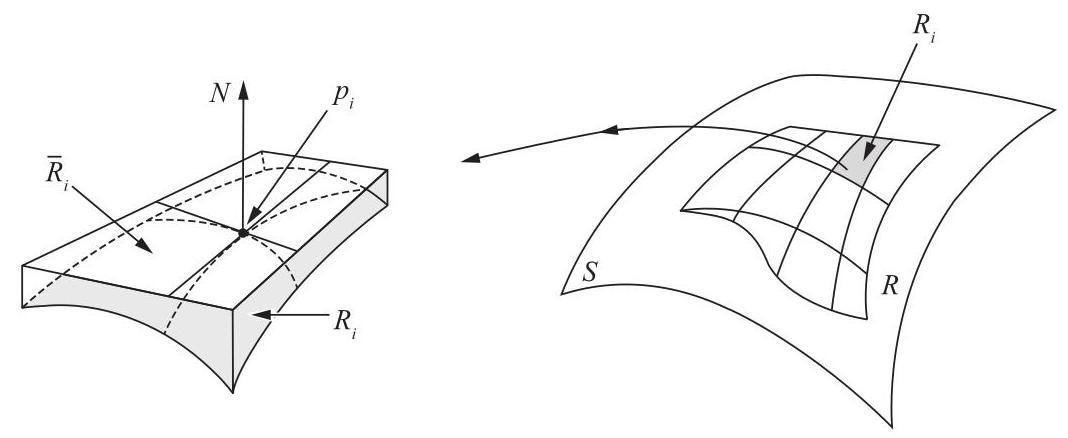
\includegraphics[max width=0.9\textwidth]{images/bo_d4b9jf3ef24c73e0334g_128_245_196_1068_438_0.jpg}
\end{center}
\hspace*{3em} 

图 2-33

给定一个划分

\[
R = \mathop{\bigcup }\limits_{i}{R}_{i}
\]

取 \(R\) 中的任意点 \({p}_{i} \in  {R}_{i}\) ，并沿在 \({p}_{i}\) 处的法线方向将 \({R}_{i}\) 投影到 \({p}_{i}\) 处的切平面上；此投影记为 \({\bar{R}}_{i}\) ，其面积记为 \(A\left( {\bar{R}}_{i}\right)\) .和 \(\mathop{\sum }\limits_{i}A\left( {\bar{R}}_{i}\right)\) 是对我们直观理解的 \(R\) 面积的近似.

如果通过选择越来越精细的分割 \({\mathfrak{P}}_{1},\ldots ,{\mathfrak{P}}_{n},\ldots\) ，并且使得 \({\mathfrak{P}}_{n}\) 的范数 \({\mu }_{n}\) 收敛于零，则存在 \(\mathop{\sum }\limits_{i}A\left( {\bar{R}}_{i}\right)\) 的极限，并且该极限与所有选择无关，那么我们说 \(R\) 的面积 \(A\left( R\right)\) 定义为

\[
A\left( R\right)  = \mathop{\lim }\limits_{{{\mu }_{n} \rightarrow  0}}\mathop{\sum }\limits_{i}A\left( {\bar{R}}_{i}\right) .
\]

关于此定义的富有启发性的讨论可在 R. Courant 的《微分和积分学》第二卷(Wiley-Interscience, New York, 1936, p. 311)中找到.

我们将证明一个有界正则曲面区域确实具有面积.我们将限制自己研究包含在坐标邻域中的有界区域，并将得到一个用第一基本形式系数表示的面积表达式，这些系数对应于该坐标系.

命题.设 \(S\) 是一个正则曲面， \(x : \mathrm{U} \rightarrow  S\) 是其上的一个坐标系，设 \(\mathbb{R} = \mathbf{x}\left( \mathrm{Q}\right)\) 是包含在 \(\mathbf{x}\left( \mathrm{U}\right)\) 中的 \(S\) 的一个有界区域.则 \(\mathbb{R}\) 的面积由下式给出

\[
\mathrm{A}\left( \mathbb{R}\right)  = {\iint }_{\mathrm{Q}}\left| {{\mathbf{x}}_{\mathrm{u}} \land  {\mathbf{x}}_{\mathrm{v}}}\right| \mathrm{{du}}\mathrm{{dv}}.
\]

证明. 考虑 \(R\) 的一个划分 \(R = \mathop{\bigcup }\limits_{i}{R}_{i}\) . 因为 \(R\) 是有界的且闭合的(因此是紧致的)，我们可以假设该划分足够精细，以至于 \({R}_{i}\) 的任意两条法线永远不相互正交.事实上，因为法线在 \(S\) 中连续变化，对于 \(p \in  R\) 中的每一个点，都存在 \(S\) 中以 \(p\) 为中心的邻域，在该邻域中任意两条法线永远不相互正交；这些邻域构成了一族覆盖 \(R\) 的开集，并且考虑一个划分，其范数小于覆盖的 Lebesgue 数(见第 2-7 节，紧致集的性质 3)，我们将满足所需条件.

固定分割中的一个区域 \({R}_{i}\) ，并选择一个点 \({p}_{i} \in  {R}_{i} = \mathbf{x}\left( {Q}_{i}\right)\) .我们想计算 \({R}_{i}\) 在 \({p}_{i}\) 处的切平面上的法向投影 \({\bar{R}}_{i}\) 的面积.为此，考虑 \({R}^{3}\) 中的一组新坐标轴 \({p}_{i}\bar{x}\bar{y}\bar{z}\) ，该坐标轴由 \({Oxyz}\) 通过一个平移 \(O{p}_{i}\) 得到，然后进行一个旋转，将 \(z\) 轴变成 \({p}_{i}\) 处的法线，同时使两个坐标系具有相同的方向(图 2-34).在新坐标系中，参数化可以写成

\[
\overline{\mathbf{x}}\left( {u,v}\right)  = \left( {\bar{x}\left( {u,v}\right) ,\bar{y}\left( {u,v}\right) ,\bar{z}\left( {u,v}\right) }\right) ,
\]

其中 \(\overline{\mathbf{x}}\left( {u,v}\right)\) 的显式形式与我们无关；只需知道向量 \(\overline{\mathbf{x}}\left( {u,v}\right)\) 是通过一个平移然后一个正交线性变换从向量 \(\mathbf{x}\left( {u,v}\right)\) 得到的.

\begin{center}
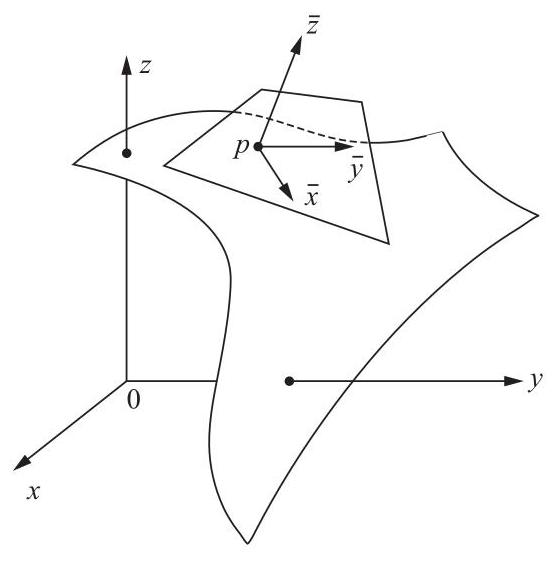
\includegraphics[max width=0.5\textwidth]{images/bo_d4b9jf3ef24c73e0334g_129_182_1060_556_562_0.jpg}
\end{center}
\hspace*{3em} 

图 2-34

我们观察到 \(\partial \left( {\bar{x},\bar{y}}\right) /\partial \left( {u,v}\right)  \neq  0\) 在 \({Q}_{i}\) 中；否则，在 \({R}_{i}\) 中的某个法向量的 \(\bar{z}\) 分量为零，并且在 \({R}_{i}\) 中存在两个正交的法线，这与我们的假设相矛盾.

\(A\left( {\bar{R}}_{i}\right)\) 的表达式由下式给出

\[
A\left( {\bar{R}}_{i}\right)  = {\iint }_{{\bar{R}}_{i}}d\bar{x}d\bar{y}.
\]

由于 \(\partial \left( {\bar{x},\bar{y}}\right) /\partial \left( {u,v}\right)  \neq  0\) ，我们可以考虑坐标变换 \(\bar{x} = \; \bar{x}\left( {u,v}\right) ,\bar{y} = \bar{y}\left( {u,v}\right)\) 并将上述表达式转换为

\[
A\left( {\bar{R}}_{i}\right)  = {\iint }_{{Q}_{i}}\frac{\partial \left( {\bar{x},\bar{y}}\right) }{\partial \left( {u,v}\right) }{dudv}.
\]

我们现在注意到，在 \({p}_{i}\) 处，向量 \({\overline{\mathbf{x}}}_{u}\) 和 \({\overline{\mathbf{x}}}_{v}\) 属于 \(\bar{x}\bar{y}\) 平面；因此，

\[
\frac{\partial \bar{z}}{\partial u} = \frac{\partial \bar{z}}{\partial v} = 0\;\text{ at }{p}_{i};
\]

因此，

\[
\left| \frac{\partial \left( {\bar{x},\bar{y}}\right) }{\partial \left( {u,v}\right) }\right|  = \left| {\frac{\partial \overline{\mathbf{x}}}{\partial u} \land  \frac{\partial \overline{\mathbf{x}}}{\partial v}}\right| \;\text{ at }{p}_{i}.
\]

由此可知

\[
\left| \frac{\partial \left( {\bar{x},\bar{y}}\right) }{\partial \left( {u,v}\right) }\right|  - \left| {\frac{\partial \bar{\mathbf{x}}}{\partial u} \land  \frac{\partial \bar{\mathbf{x}}}{\partial v}}\right|  = {\epsilon }_{i}\left( {u,v}\right) ,\;\left( {u,v}\right)  \in  {Q}_{i},
\]

其中 \({\epsilon }_{i}\left( {u,v}\right)\) 是 \({Q}_{i}\) 中具有 \({\epsilon }_{i}\left( {{\mathbf{x}}^{-1}\left( {p}_{i}\right) }\right)  = 0\) 的连续函数.由于向量的长度在平移和正交线性映射下保持不变，我们得到

\[
\left| {\frac{\partial \mathbf{x}}{\partial u} \land  \frac{\partial \mathbf{x}}{\partial v}}\right|  = \left| {\frac{\partial \overline{\mathbf{x}}}{\partial u} \land  \frac{\partial \overline{\mathbf{x}}}{\partial v}}\right|  = \left| \frac{\partial \left( {\bar{x},\bar{y}}\right) }{\partial \left( {u,v}\right) }\right|  - {\epsilon }_{i}\left( {u,v}\right) .
\]

现在设 \({M}_{i}\) 和 \({m}_{i}\) 是连续函数 \({\epsilon }_{i}\left( {u,v}\right)\) 在紧区域 \({Q}_{i}\) 中的最大值和最小值；因此，

\[
{m}_{i} \leq  \left| \frac{\partial \left( {\bar{x},\bar{y}}\right) }{\partial \left( {u,v}\right) }\right|  - \left| {\frac{\partial \mathbf{x}}{\partial u} \land  \frac{\partial \mathbf{x}}{\partial v}}\right|  \leq  {M}_{i};
\]

因此，

\[
{m}_{i}{\iint }_{{Q}_{i}}{dudv} \leq  A\left( {\bar{R}}_{i}\right)  - {\iint }_{{Q}_{i}}\left| {\frac{\partial \mathbf{x}}{\partial u} \land  \frac{\partial \mathbf{x}}{\partial v}}\right| {dudv} \leq  {M}_{i}{\iint }_{{Q}_{i}}{dudv}.
\]

对所有 \({R}_{i}\) 执行相同的操作，我们得到

\[
\mathop{\sum }\limits_{i}{m}_{i}A\left( {Q}_{i}\right)  \leq  \mathop{\sum }\limits_{i}A\left( {\bar{R}}_{i}\right)  - {\iint }_{Q}\left| {{\mathbf{x}}_{u} \land  {\mathbf{x}}_{v}}\right| {dudv} \leq  \mathop{\sum }\limits_{i}{M}_{i}A\left( {Q}_{i}\right) .
\]

现在，越来越精细地细分给定的分区，使得范数 \(\mu  \rightarrow  0\) .然后 \({M}_{i} \rightarrow  {m}_{i}\) .因此， \(\mathop{\sum }\limits_{i}A\left( {\bar{R}}_{i}\right)\) 的极限存在，由下式给出:

\[
A\left( R\right)  = {\iint }_{Q}\left| {\frac{\partial \mathbf{x}}{\partial u} \land  \frac{\partial \mathbf{x}}{\partial v}}\right| {dudv}
\]

这显然与分区的选择以及每个分区中的点 \({p}_{i}\) 的选择无关.证毕.

附录 A 连续性和可微性简要回顾

\({R}^{n}\) 表示实数 \(n\) 元组 \(\left( {{x}_{1},\ldots ,{x}_{n}}\right)\) 的集合.尽管我们只使用 \({R}^{1} = R,{R}^{2}\) 和 \({R}^{3}\) 的情况，但更一般的 \({R}^{n}\) 概念统一了定义并且不会带来额外的困难；如果读者愿意，可以将其视为 \({R}^{2}\) 或 \({R}^{3}\) .在这些特定情况下，我们将使用以下更传统的符号: \(x\) 或 \(t\) 表示 \(R,\left( {x,y}\right)\) 或 \(\left( {u,v}\right)\) 表示 \({R}^{2}\) ，以及 \(\left( {x,y,z}\right)\) 表示 \({R}^{3}\) .

\section*{A. \({R}^{n}\) 中的连续性}

我们首先精确地定义一个点与给定点 \({p}_{0} \in  {R}^{n}\) 之间的 \(\epsilon\) -接近程度.

在 \({R}^{n}\) 中，以 \({p}_{0} = \left( {{x}_{1}^{0},\ldots ,{x}_{n}^{0}}\right)\) 为中心、半径为 \(\epsilon  > 0\) 的球(或开球)是集合

\[
{B}_{\epsilon }\left( {p}_{0}\right)  = \left\{  {\left( {{x}_{1},\ldots ,{x}_{n}}\right)  \in  {R}^{n};{\left( {x}_{1} - {x}_{1}^{0}\right) }^{2} + \cdots  + {\left( {x}_{n} - {x}_{n}^{0}\right) }^{2} < {\epsilon }^{2}}\right\}  .
\]

因此，在 \(R,{B}_{\epsilon }\left( {p}_{0}\right)\) 中是一个以 \({p}_{0}\) 为中心、长度为 \({2\epsilon }\) 的开区间；在 \({R}^{2}\) 中， \({B}_{\epsilon }\left( {p}_{0}\right)\) 是一个以 \({p}_{0}\) 为中心、半径为 \(\epsilon\) 的圆盘的内部；在 \({R}^{3},{B}_{\epsilon }\left( {p}_{0}\right)\) 中，是围绕一个以 \({p}_{0}\) 为中心、半径为 \(\epsilon\) 的球的区域的内部(见图 A2-1).

如果对于每个 \(p \in  U\) 都存在一个球 \({B}_{\epsilon }\left( p\right)  \subset  U\) ，则称集合 \(U \subset  {R}^{n}\) 是一个开集；直观上这意味着 \(U\) 中的点被 \(U\) 中的点完全包围，或者足够接近 \(U\) 中的点的点仍然属于 \(U\) .

例如，集合

\[
\left\{  {\left( {x,y}\right)  \in  {R}^{2};a < x < b,c < y < d}\right\}
\]

很容易看出在 \({R}^{2}\) 中是开集.然而，如果其中一个严格不等式，例如 \(x < b\) ，被 \(x \leq  b\) 取代，则该集合不再是开集；以属于该集合的点 \(\left( {b,\left( {d + c}\right) /2}\right)\) 为中心、包含在该集合中的任何球都不能包含在该集合中(图 A2-2).

\begin{center}
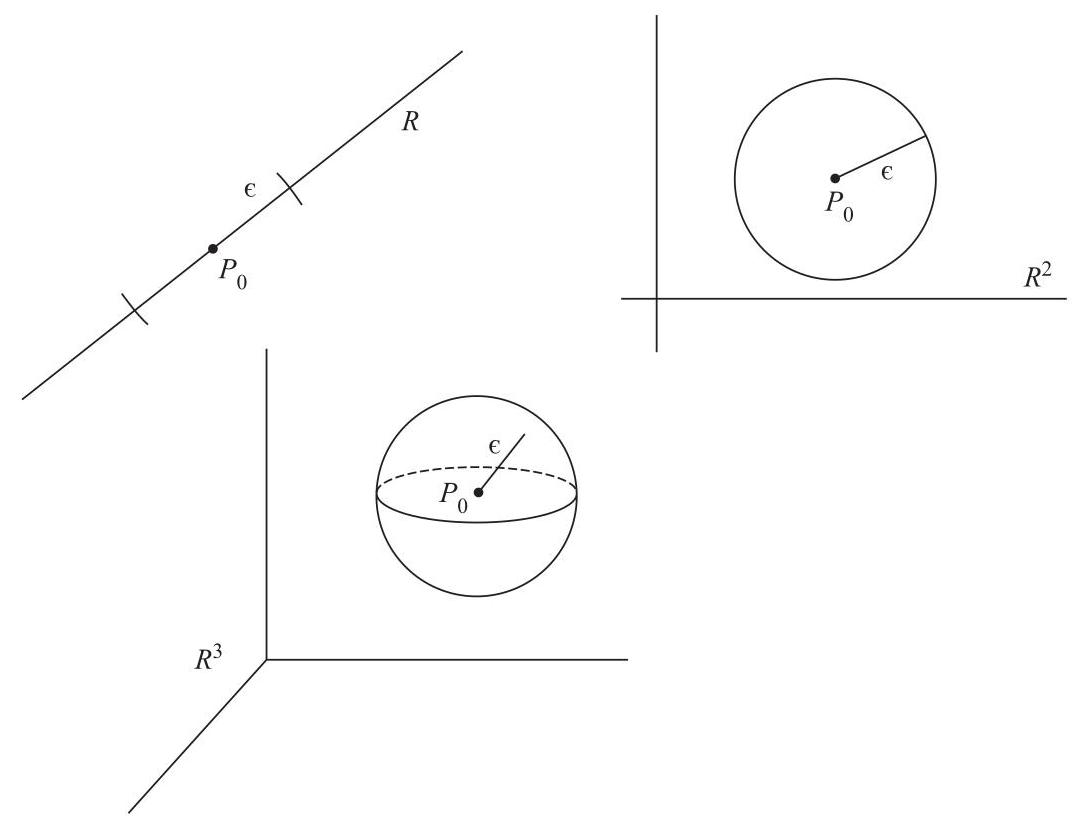
\includegraphics[max width=0.9\textwidth]{images/bo_d4b9jf3ef24c73e0334g_132_243_191_1083_824_0.jpg}
\end{center}
\hspace*{3em} 

图 A2-1

为了方便起见，我们说包含点 \(p \in  {R}^{n}\) 的 \({R}^{n}\) 中的开集是 \(p\) 的邻域.

从现在开始， \(U \subset  {R}^{n}\) 将表示 \({R}^{n}\) 中的一个开集.

我们回顾一下，一个实变量的实函数 \(f : U \subset  R \rightarrow  R\) 在 \({x}_{0} \in  U\) 处是连续的，如果给定一个 \(\epsilon  > 0\) ，存在一个 \(\delta  > 0\) ，使得如果 \(\left| {x - {x}_{0}}\right|  < \; \delta\) ，则

\[
\left| {f\left( x\right)  - f\left( {x}_{0}\right) }\right|  < \epsilon
\]

\begin{center}
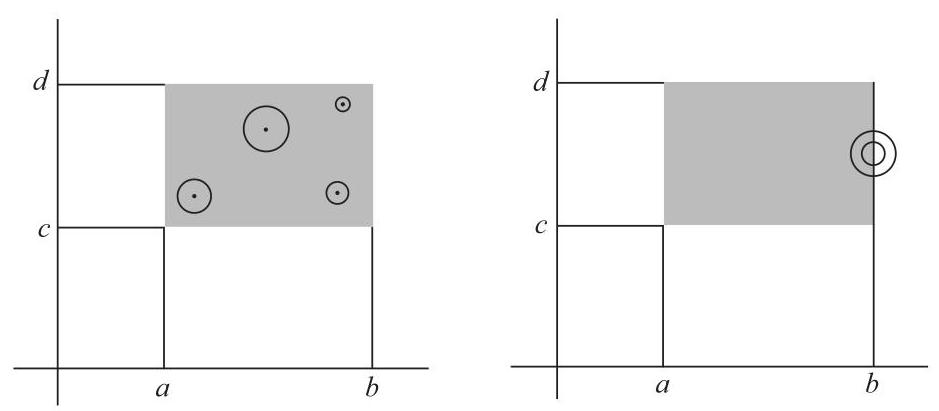
\includegraphics[max width=0.8\textwidth]{images/bo_d4b9jf3ef24c73e0334g_132_316_1628_939_411_0.jpg}
\end{center}
\hspace*{3em} 

图 A2-2

类似地，一个二元实函数的实函数 \(f : U \subset  {R}^{2} \rightarrow  R\) 在 \(\left( {{x}_{0},{y}_{0}}\right)  \in  U\) 处是连续的，如果给定一个 \(\epsilon  > 0\) ，存在一个 \(\delta  > 0\) ，使得如果 \({\left( x - {x}_{0}\right) }^{2} + {\left( y - {y}_{0}\right) }^{2} < {\delta }^{2}\) ，则

\[
\left| {f\left( {x,y}\right)  - f\left( {{x}_{0},{y}_{0}}\right) }\right|  < \epsilon .
\]

球的概念将这些定义统一为以下一般概念的特例:

一个映射 \(F : U \subset  {R}^{n} \rightarrow  {R}^{m}\) 在 \(p \in  U\) 处是连续的，如果给定 \(\epsilon  > 0\) ，存在一个 \(\delta  > 0\) ，使得

\[
F\left( {{B}_{\delta }\left( p\right) }\right)  \subset  {B}_{\epsilon }\left( {F\left( p\right) }\right) .
\]

换句话说， \(F\) 在 \(p\) 处是连续的，如果任意接近 \(F\left( p\right)\) 的点是任意接近 \(p\) 的点的像.很容易看出，在 \(n = 1,2\) 和 \(m = 1\) 的特例中，这与之前的定义一致.我们说 \(F\) 在 \(U\) 中是连续的，如果 \(F\) 对于所有 \(p \in  U\) 都是连续的(图 A2-3).

\begin{center}
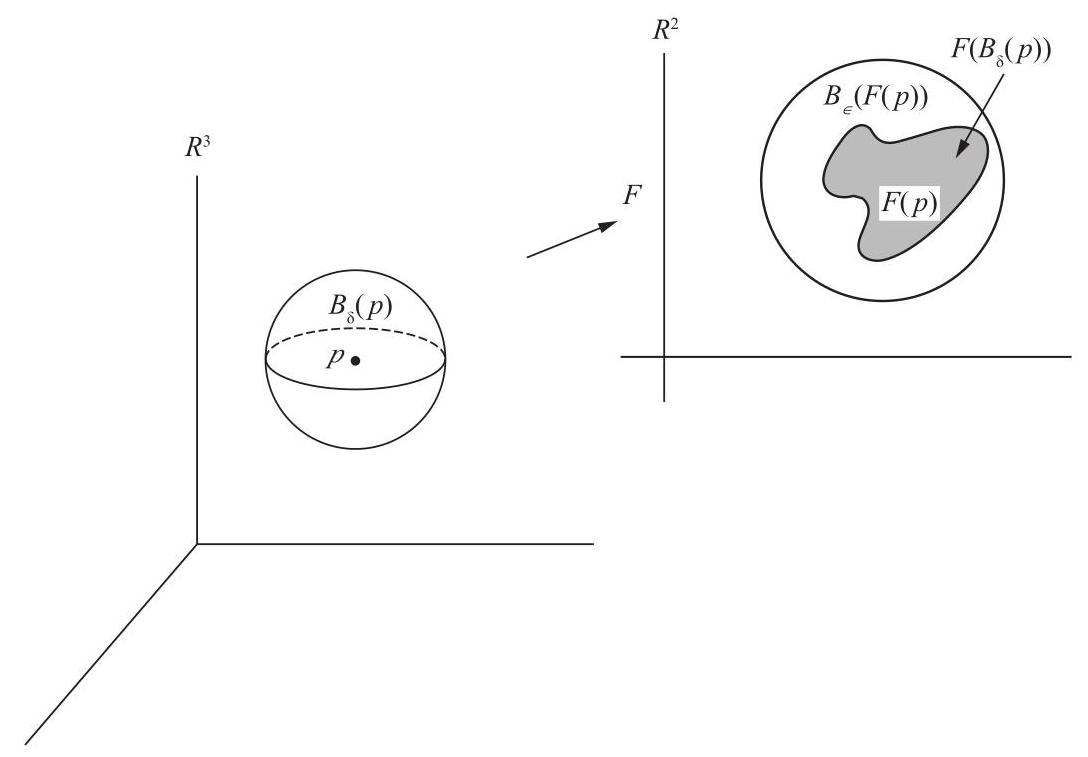
\includegraphics[max width=0.9\textwidth]{images/bo_d4b9jf3ef24c73e0334g_133_218_1013_1088_757_0.jpg}
\end{center}
\hspace*{3em} 

图 A2-3

给定一个映射 \(F : U \subset  {R}^{n} \rightarrow  {R}^{m}\) ，我们可以如下确定 \(n\) 个变量的 \(m\) 函数.令 \(p = \left( {{x}_{1},\ldots ,{x}_{n}}\right)  \in  U\) 和 \(f\left( p\right)  = \left( {{y}_{1},\ldots ,{y}_{m}}\right)\) .那么我们可以写成

\[
{y}_{1} = {f}_{1}\left( {{x}_{1},\ldots ,{x}_{n}}\right) ,\ldots ,{y}_{m} = {f}_{m}\left( {{x}_{1},\ldots ,{x}_{n}}\right) .
\]

函数 \({f}_{i} : U \rightarrow  R,i = 1,\ldots ,m\) 是 \(F\) 的分量函数.

例 1 (对称性).令 \(F : {R}^{3} \rightarrow  {R}^{3}\) 为将每个 \(p \in  {R}^{3}\) 映射到关于原点 \(O \in  {R}^{3}\) 对称的点 \(p\) 的映射.则 \(F\left( p\right)  =  - p\) ，或

\[
F\left( {x,y,z}\right)  = \left( {-x, - y, - z}\right) ,
\]

而 \(F\) 的分量函数是

\[
{f}_{1}\left( {x,y,z}\right)  =  - x,\;{f}_{2}\left( {x,y,z}\right)  =  - y,\;{f}_{3}\left( {x,y,z}\right)  =  - z.
\]

例 2 (反演).令 \(F : {R}^{2} - \{ \left( {0,0}\right) \}  \rightarrow  {R}^{2}\) 定义如下.用 \(\left( {0,0}\right)  = O\) 表示点 \(p \in  {R}^{2}\) 到原点 \(\left| p\right|\) 的距离.根据定义， \(F\left( p\right) ,p \neq  0\) 属于半直线 \({Op}\) 并且满足 \(\left| {F\left( p\right) }\right|\) . \(\left| p\right|  = 1\) .因此， \(F\left( p\right)  = p/{\left| p\right| }^{2}\) ，或

\[
F\left( {x,y}\right)  = \left( {\frac{x}{{x}^{2} + {y}^{2}},\frac{y}{{x}^{2} + {y}^{2}}}\right) ,\;\left( {x,y}\right)  \neq  \left( {0,0}\right) ,
\]

而 \(F\) 的分量函数是

\[
{f}_{1}\left( {x,y}\right)  = \frac{x}{{x}^{2} + {y}^{2}},\;{f}_{2}\left( {x,y}\right)  = \frac{y}{{x}^{2} + {y}^{2}}.
\]

例 3 (投影).令 \(\pi  : {R}^{3} \rightarrow  {R}^{2}\) 为投影 \(\pi \left( {x,y,z}\right)  = \; \left( {x,y}\right)\) .则 \({f}_{1}\left( {x,y,z}\right)  = x,{f}_{2}\left( {x,y,z}\right)  = y\) .

下面的命题表明映射 \(F\) 的连续性等价于其分量函数的连续性.

命题 1.F: \(\mathrm{U} \subset  {\mathbb{R}}^{N} \rightarrow  {\mathbb{R}}^{\mathrm{m}}\) 是连续的当且仅当每个分量函数 \({\mathrm{f}}_{\mathrm{i}} : \mathrm{U} \subset  {\mathbb{R}}^{N} \rightarrow  \mathbb{R},\mathrm{i} = 1,\ldots ,\mathrm{m}\) 是连续的.

证明.假设 \(F\) 在 \(p \in  U\) 处连续.则给定 \(\epsilon  > 0\) ，存在 \(\delta  > 0\) 使得 \(F\left( {{B}_{\delta }\left( p\right) }\right)  \subset  {B}_{\epsilon }\left( {F\left( p\right) }\right)\) .因此，如果 \(q \in  {B}_{\delta }\left( p\right)\) ，则

\[
F\left( q\right)  \in  {B}_{\epsilon }\left( {F\left( p\right) }\right) ,
\]

即，

\[
{\left( {f}_{1}\left( q\right)  - {f}_{1}\left( p\right) \right) }^{2} + \cdots  + {\left( {f}_{m}\left( q\right)  - {f}_{m}\left( p\right) \right) }^{2} < {\epsilon }^{2},
\]

这意味着，对于每个 \(i = 1,\ldots ,m,\left| {{f}_{i}\left( q\right)  - {f}_{i}\left( p\right) }\right|  < \epsilon\) .因此，给定 \(\epsilon  > 0\) 存在 \(\delta  > 0\) 使得如果 \(q \in  {B}_{\delta }\left( p\right)\) ，则 \(\left| {{f}_{i}\left( q\right)  - {f}_{i}\left( p\right) }\right|  < \epsilon\) .因此，每个 \({f}_{i}\) 在 \(p\) 处是连续的.

反之，设 \({f}_{i},i = 1,\ldots ,m\) 在 \(p\) 处连续.则给定 \(\epsilon  > 0\) 存在 \({\delta }_{i} > 0\) 使得如果 \(q \in  {B}_{{\delta }_{i}}\left( p\right)\) ，则 \(\left| {{f}_{i}\left( q\right)  - {f}_{i}\left( p\right) }\right|  < \epsilon /\sqrt{m}\) .令 \(\delta  < \min {\delta }_{i}\) 并设 \(q \in  {B}_{\delta }\left( p\right)\) .则

\[
{\left( {f}_{1}\left( q\right)  - {f}_{1}\left( p\right) \right) }^{2} + \cdots  + {\left( {f}_{m}\left( q\right)  - {f}_{m}\left( p\right) \right) }^{2} < {\epsilon }^{2},
\]

从而证明了 \(F\) 在 \(p\) 处的连续性.Q.E.D.

由此可知，示例 1、2 和 3 中的映射是连续的.

示例 4. 设 \(F : U \subset  R \rightarrow  {R}^{m}\) .则

\[
F\left( t\right)  = \left( {{x}_{1}\left( t\right) ,\ldots ,{x}_{m}\left( t\right) }\right) ,\;t \in  U.
\]

这通常称为向量值函数，而 \(F\) 的分量函数是向量 \(F\left( t\right)  \in  {R}^{m}\) 的分量.当 \(F\) 连续，或者等价地，函数 \({x}_{i}\left( t\right) ,i = 1,\ldots ,m\) 连续时，我们说 \(F\) 是 \({R}^{m}\) 中的一条连续曲线.

在大多数应用中，用邻域而不是球来表示连续性更为方便.

命题 2. 映射 \(\mathrm{F} : \mathrm{U} \subset  {\mathbb{R}}^{N} \rightarrow  {\mathbb{R}}^{\mathrm{m}}\) 在 \(\mathrm{p} \in  \mathrm{U}\) 处连续当且仅当，给定 \({\mathbb{R}}^{\mathrm{m}}\) 中 \(\mathrm{F}\left( \mathrm{p}\right)\) 的一个邻域 \(\mathrm{V}\) ，存在 \({\mathbb{R}}^{N}\) 中 \(\mathrm{p}\) 的一个邻域 \(\mathrm{W}\) 使得 \(\mathrm{F}\left( \mathrm{W}\right)  \subset  \mathrm{V}\) .

证明.假设 \(F\) 在 \(p\) 处连续.由于 \(V\) 是包含 \(F\left( p\right)\) 的开集，它包含某个 \(\epsilon  > 0\) 的一个球 \({B}_{\epsilon }\left( {F\left( p\right) }\right)\) .根据连续性，存在一个球 \({B}_{\delta }\left( p\right)  = W\) 使得

\[
F\left( W\right)  = F\left( {{B}_{\delta }\left( p\right) }\right)  \subset  {B}_{\epsilon }\left( {F\left( p\right) }\right)  \subset  V,
\]

这证明了该条件是必要条件.

反之，假设条件成立.设给定 \(\varepsilon  > 0\) 并令 \(V = {B}_{\epsilon }\left( {F\left( p\right) }\right)\) .根据假设，存在 \({R}^{n}\) 中 \(p\) 的一个邻域 \(W\) 使得 \(F\left( W\right)  \subset  V\) .由于 \(W\) 是开集，存在一个球 \({B}_{\delta }\left( p\right)  \subset  W\) .因此，

\[
F\left( {{B}_{\delta }\left( p\right) }\right)  \subset  F\left( W\right)  \subset  V = {B}_{\epsilon }\left( {F\left( p\right) }\right) ,
\]

从而证明了 \(F\) 在 \(p\) 处的连续性.Q.E.D.

连续映射的复合产生连续映射.更精确地说，我们有以下命题.

命题 3. 设 \(\mathrm{F} : \mathrm{U} \subset  {\mathbb{R}}^{N} \rightarrow  {\mathbb{R}}^{\mathrm{m}}\) 和 \(\mathrm{G} : \mathrm{V} \subset  {\mathbb{R}}^{\mathrm{m}} \rightarrow  {\mathbb{R}}^{\mathrm{k}}\) 是连续映射，其中 \(\mathrm{U}\) 和 \(\mathrm{V}\) 是开集，且 \(\mathrm{F}\left( \mathrm{U}\right)  \subset  \mathrm{V}\) .则 \(\mathrm{G} \circ  \mathrm{F} : \mathrm{U} \subset  {\mathbb{R}}^{N} \rightarrow  {\mathbb{R}}^{\mathrm{k}}\) 是一个连续映射.

证明. 设 \(p \in  U\) ，且设 \({W}_{1}\) 是 \({R}^{k}\) 中 \(G \circ  F\left( p\right)\) 的一个邻域.由 \(G\) 的连续性，存在 \({R}^{m}\) 中 \(F\left( p\right)\) 的一个邻域 \(Q\) ，使得 \(G\left( Q\right)  \subset  {W}_{1}\) .由 \(F\) 的连续性，存在 \({R}^{n}\) 中 \(\left( p\right)\) 的一个邻域 \({W}_{2}\) ，使得 \(F\left( {W}_{2}\right)  \subset  Q\) .因此，

\[
G \circ  F\left( {W}_{2}\right)  \subset  G\left( Q\right)  \subset  {W}_{1},
\]

以及因此 \(G \circ  F\) 的连续性.Q.E.D.

通常有必要处理定义在 \({R}^{n}\) 的任意(不一定是开的)集合上的映射.为了将前面的思想扩展到这种情况，我们将按如下方式进行.

设 \(F : A \subset  {R}^{n} \rightarrow  {R}^{m}\) 是一个映射，其中 \(A\) 是 \({R}^{n}\) 中的一个任意集合.如果给定 \({R}^{m}\) 中 \(F\left( p\right)\) 的一个邻域 \(V\) ，存在 \({R}^{n}\) 中 \(p\) 的一个邻域 \(W\) ，使得 \(F\left( {W \cap  A}\right)  \subset  V\) ，则称 \(F\) 在 \(p \in  A\) 处是连续的.为此，将 \(A\) 中 \(p\) 的邻域称为 \(W \cap  A\) 是方便的.当对于每个点 \(p \in  B\) ，存在一个完全包含在 \(B\) 中的 \(A\) 中 \(p\) 的邻域时，集合 \(B \subset  A\) 是开的.

\begin{center}
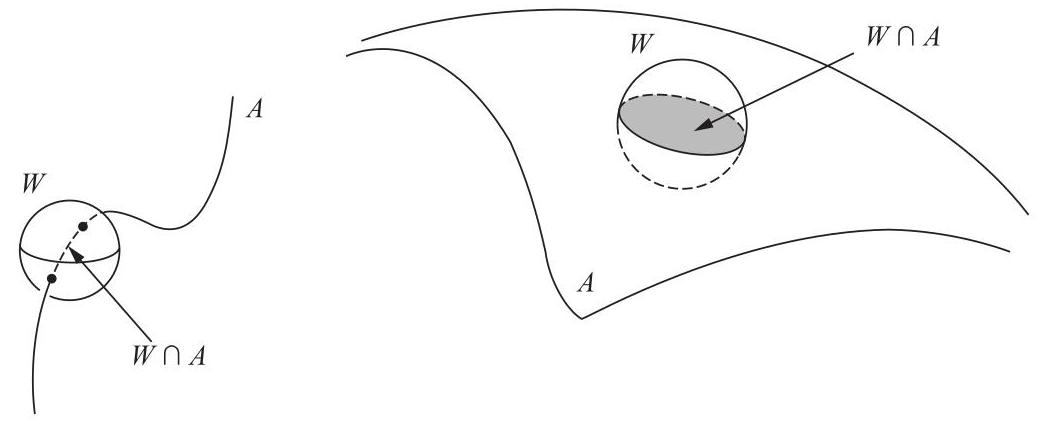
\includegraphics[max width=0.9\textwidth]{images/bo_d4b9jf3ef24c73e0334g_136_260_508_1048_425_0.jpg}
\end{center}
\hspace*{3em} 

图 A2-4

例 5. 设

\[
E = \left\{  {\left( {x,y,z}\right)  \in  {R}^{3};\frac{{x}^{2}}{{a}^{2}} + \frac{{y}^{2}}{{b}^{2}} + \frac{{z}^{2}}{{c}^{2}} = 1}\right\}
\]

是一个椭球体，设 \(\pi  : {R}^{3} \rightarrow  {R}^{2}\) 是例 3 的投影.则 \(\pi\) 在 \(E\) 上的限制是从 \(E\) 到 \({R}^{2}\) 的一个连续映射.

我们称连续映射 \(F : A \subset  {R}^{n} \rightarrow  {R}^{n}\) 是到 \(F\left( A\right)\) 的同胚，如果 \(F\) 是单射且逆映射 \({F}^{-1} : F\left( A\right)  \subset  {R}^{n} \rightarrow  {R}^{n}\) 是连续的.在这种情况下， \(A\) 和 \(F\left( A\right)\) 是同胚集.

例 6. 设 \(F : {R}^{3} \rightarrow  {R}^{3}\) 由下式给出

\[
F\left( {x,y,z}\right)  = \left( {{xa},{yb},{zc}}\right) .
\]

\(F\) 显然是连续的，并且 \(F\) 在球面上的限制

\[
{S}^{2} = \left\{  {\left( {x,y,z}\right)  \in  {R}^{3};{x}^{2} + {y}^{2} + {z}^{2} = 1}\right\}
\]

是一个连续映射 \(\widetilde{F} : {S}^{2} \rightarrow  {R}^{3}\) .注意 \(\widetilde{F}\left( {S}^{2}\right)  = E\) ，其中 \(E\) 是例 5 的椭球体.也很清楚 \(F\) 是单射并且

\[
{F}^{-1}\left( {x,y,z}\right)  = \left( {\frac{x}{a},\frac{y}{b},\frac{z}{c}}\right) .
\]

因此， \({\widetilde{F}}^{-1} = {F}^{-1} \mid  E\) 是连续的.所以， \(\widetilde{F}\) 是从球面 \({S}^{2}\) 到椭球体 \(E\) 的一个同胚.

最后，我们想描述定义在闭区间 \(\left\lbrack  {a,b}\right\rbrack\) 上的实连续函数的两个性质，

\[
\left\lbrack  {a,b}\right\rbrack   = \{ x \in  R;a \leq  x \leq  b\}
\]

(下面的命题 4 和 5)，以及闭区间 \(\left\lbrack  {a,b}\right\rbrack\) 本身的一个重要性质.它们将在本书中反复使用.

命题 4(介值定理).设 f: [a, b] \(\rightarrow\) R 是定义在闭区间 [a, b] 上的连续函数.假设 \(\mathrm{f}\left( \mathrm{a}\right)\) 和 \(\mathrm{f}\left( \mathrm{b}\right)\) 符号相反；即， \(\mathrm{f}\left( \mathrm{a}\right) \mathrm{f}\left( \mathrm{b}\right)  < 0\) .则存在一点 \(c \in  \left( {a,b}\right)\) 使得 \(\mathrm{f}\left( \mathrm{c}\right)  = 0\) .

命题 5.设 \(\mathrm{f} : \left\lbrack  {\mathrm{a},\mathrm{b}}\right\rbrack\) 是定义在闭区间 \(\left\lbrack  {\mathrm{a},\mathrm{b}}\right\rbrack\) 上的连续函数.则 \(\mathrm{f}\) 在 \(\left\lbrack  {\mathrm{a},\mathrm{b}}\right\rbrack\) 中达到其最大值和最小值；即，存在点 \({x}_{1},{x}_{2} \in  \left\lbrack  {\mathrm{a},\mathrm{b}}\right\rbrack\) 使得对于所有 \(x \in  \left\lbrack  {\mathrm{a},\mathrm{b}}\right\rbrack\) ，都有 \(\mathrm{f}\left( {x}_{1}\right)  < \mathrm{f}\left( x\right)  < \mathrm{f}\left( {x}_{2}\right)\) .

命题 6(Heine-Borel 定理).设 \(\left\lbrack  {\mathrm{a},\mathrm{b}}\right\rbrack\) 是一个闭区间，设 \({\mathrm{I}}_{\alpha },\alpha  \in  \mathrm{A}\) 是一个开区间集合，使得 \(\mathop{\bigcup }\limits_{\alpha }{\mathrm{I}}_{\alpha } \supset  \left\lbrack  {\mathrm{a},\mathrm{b}}\right\rbrack\) .则可以选取有限个 \({\mathrm{I}}_{{\mathrm{k}}_{1}},{\mathrm{I}}_{{\mathrm{k}}_{2}},\ldots ,{\mathrm{I}}_{{\mathrm{k}}_{N}}\) 个 \({\mathrm{I}}_{\alpha }\) 使得 \(\mathop{\bigcup }\limits_{{\mathrm{k}}_{\mathrm{i}}}{\mathrm{I}}_{{\mathrm{k}}_{\mathrm{i}}} \supset \; \left\lbrack  {\mathrm{a},\mathrm{b}}\right\rbrack  ,\mathrm{i} = 1,\ldots ,N\) .

这些命题是高等微积分课程中的标准定理，我们在此不予证明.然而，证明在第 5 章的附录中提供(分别是命题 8、13 和 11).

\section*{B. \({R}^{n}\) 中的可微性}

设 \(f : U \subset  R \rightarrow  R\) . \(f\) 在 \({x}_{0} \in  U\) 处的导数 \({f}^{\prime }\left( {x}_{0}\right)\) 是极限(如果存在)

\[
{f}^{\prime }\left( {x}_{0}\right)  = \mathop{\lim }\limits_{{h \rightarrow  0}}\frac{f\left( {{x}_{0} + h}\right)  - f\left( {x}_{0}\right) }{h},\;{x}_{0} + h \in  U.
\]

当 \(f\) 在 \({x}_{0}\) 的邻域 \(V\) 的所有点处都有导数时，我们可以考虑 \({f}^{\prime } : V \rightarrow  R\) 在 \({x}_{0}\) 处的导数，这被称为 \(f\) 在 \({x}_{0}\) 处的二阶导数 \({f}^{\prime \prime }\left( {x}_{0}\right)\) ，依此类推.如果 \(f\) 在 \({x}_{0}\) 处具有各阶连续导数，则称 \(f\) 在 \({x}_{0}\) 处可微.如果 \(f\) 在 \(U\) 内的所有点处都可微，则称 \(f\) 在 \(U\) 内可微.

注.我们使用“可微”一词来表示有时称为“无穷可微”(或属于 \({C}^{\infty }\) 类)的概念.我们的用法不应与初等微积分中的用法混淆，在初等微积分中，如果一个函数的一阶导数存在，则称该函数是可微的.

设 \(F : U \subset  {R}^{2} \rightarrow  R\) . \(\mathrm{f}\) 关于 \(x\) 在 \(\left( {{x}_{0},{y}_{0}}\right)  \in  U\) 处的偏导数，记作 \(\left( {\partial f/\partial x}\right) \left( {{x}_{0},{y}_{0}}\right)\) ，(当它存在时)是函数 \(x \rightarrow  f\left( {x,{y}_{0}}\right)\) 的一元函数在 \({x}_{0}\) 处的导数.类似地，关于 \(y\) 在 \(\left( {{x}_{0},{y}_{0}}\right) ,\left( {\partial f/\partial y}\right) \left( {{x}_{0},{y}_{0}}\right)\) 处的偏导数，定义为函数 \(y \rightarrow  f\left( {{x}_{0},y}\right)\) 在 \({y}_{0}\) 处的导数.当 \(f\) 在 \(\left( {{x}_{0},{y}_{0}}\right)\) 的邻域 \(V\) 的所有点上都存在偏导数时，我们可以考虑 \(\left( {{x}_{0},{y}_{0}}\right)\) 处的二阶偏导数:

\[
\frac{\partial }{\partial x}\left( \frac{\partial f}{\partial x}\right)  = \frac{{\partial }^{2}f}{\partial {x}^{2}},\;\frac{\partial }{\partial x}\left( \frac{\partial f}{\partial y}\right)  = \frac{{\partial }^{2}f}{\partial x\partial y},
\]

\[
\frac{\partial }{\partial y}\left( \frac{\partial f}{\partial x}\right)  = \frac{{\partial }^{2}f}{\partial y\partial x},\;\frac{\partial }{\partial y}\left( \frac{\partial f}{\partial y}\right)  = \frac{{\partial }^{2}f}{\partial {y}^{2}},
\]

依此类推.如果 \(f\) 在 \(\left( {{x}_{0},{y}_{0}}\right) .f\) 处具有所有阶的连续偏导数，则称 \(f\) 在 \(\left( {{x}_{0},{y}_{0}}\right)\) 处可微；如果 \(f\) 在 \(U\) 的所有点处都可微，则称 \(f\) 在 \(U\) 中可微.我们有时用以下方式表示偏导数:

\[
\frac{\partial f}{\partial x} = {f}_{x},\;\frac{\partial f}{\partial y} = {f}_{y},\;\frac{{\partial }^{2}f}{\partial {x}^{2}} = {f}_{xx},\;\frac{{\partial }^{2}f}{\partial x\partial y} = {f}_{xy},\;\frac{{\partial }^{2}f}{\partial {y}^{2}} = {f}_{yy}.
\]

一个重要的事实是，当 \(f\) 可微时， \(f\) 的偏导数与它们的执行顺序无关；也就是说，

\[
\frac{{\partial }^{2}f}{\partial x\partial y} = \frac{{\partial }^{2}f}{\partial y\partial x},\;\frac{{\partial }^{3}f}{{\partial }^{2}x\partial y} = \frac{{\partial }^{3}f}{\partial x\partial y\partial x},\;\text{ etc. }
\]

偏导数和可微性的定义可以很容易地推广到函数 \(f : U \subset  {R}^{n} \rightarrow  R\) .例如， \(\left( {\partial f/\partial {x}_{3}}\right) \left( {{x}_{1}^{0},{x}_{2}^{0},\ldots ,{x}_{n}^{0}}\right)\) 是函数的一元函数

\[
{x}_{3} \rightarrow  f\left( {{x}_{1}^{0},{x}_{2}^{0},{x}_{3},{x}_{4}^{0},\ldots ,{x}_{n}^{0}}\right) .
\]

另一个重要的事实是，偏导数遵循所谓的链式法则.例如，如果 \(x = x\left( {u,v}\right) ,y = y\left( {u,v}\right) ,z = z\left( {u,v}\right)\) 是 \(U \subset  {R}^{2}\) 中的实可微函数，而 \(f\left( {x,y,z}\right)\) 是 \({R}^{3}\) 中的实可微函数，那么复合函数 \(f\left( {x\left( {u,v}\right) ,y\left( {u,v}\right) ,z\left( {u,v}\right) }\right)\) 是 \(U\) 中的可微函数，并且 \(f\) 关于，比如说， \(u\) 的偏导数由下式给出:

\[
\frac{\partial f}{\partial u} = \frac{\partial f}{\partial x}\frac{\partial x}{\partial u} + \frac{\partial f}{\partial y}\frac{\partial y}{\partial u} + \frac{\partial f}{\partial z}\frac{\partial z}{\partial u}.
\]

我们现在有兴趣将可微性的概念推广到映射 \(F : U \subset  {R}^{n} \rightarrow  {R}^{m}\) .我们说，如果它的分量函数在 \(p\) 处可微，则 \(F\) 在 \(p \in  U\) 处可微；也就是说，通过写出

\[
F\left( {{x}_{1},\ldots ,{x}_{n}}\right)  = \left( {{f}_{1}\left( {{x}_{1},\ldots ,{x}_{n}}\right) ,\ldots ,{f}_{m}\left( {{x}_{1},\ldots ,{x}_{n}}\right) }\right) ,
\]

函数 \({f}_{i},i = 1,\ldots ,m\) 在 \(p.F\) 处具有所有阶的连续偏导数，如果在 \(U\) 中的所有点都可微，则在 \(U\) 中是可微的.

对于 \(m = 1\) 的情况，这重复了之前的定义.对于 \(n = 1\) 的情况，我们得到了 \({R}^{m}\) 中(参数化)可微曲线的概念.在第 1 章中，我们已经看到了 \({R}^{3}\) 中的这样一个对象.为了我们的目的，我们需要将第 1 章的切向量定义扩展到当前情况.映射 \(\alpha  : U \subset  R \rightarrow  {R}^{m}\) 在 \({t}_{0} \in  U\) 处的切向量是 \({R}^{m}\) 中的向量

\[
{\alpha }^{\prime }\left( {t}_{0}\right)  = \left( {{x}_{1}^{\prime }\left( {t}_{0}\right) ,\ldots ,{x}_{m}^{\prime }\left( {t}_{0}\right) }\right) .
\]

例 7. 设 \(F : U \subset  {R}^{2} \rightarrow  {R}^{3}\) 由下式给出

\[
F\left( {u,v}\right)  = \left( {\cos u\cos v,\cos u\sin v,{\cos }^{2}v}\right) ,\;\left( {u,v}\right)  \in  U.
\]

\(F\) 的分量函数，即，

\[
{f}_{1}\left( {u,v}\right)  = \cos u\cos v,\;{f}_{2}\left( {u,v}\right)  = \cos u\sin v,\;{f}_{3}\left( {u,v}\right)  = {\cos }^{2}v
\]

在 \(U\) 中具有所有阶的连续偏导数.因此， \(F\) 在 \(U\) 中是可微的.

例 8. 设 \(\alpha  : U \subset  R \rightarrow  {R}^{4}\) 由下式给出

\[
\alpha \left( t\right)  = \left( {{t}^{4},{t}^{3},{t}^{2},t}\right) ,\;t \in  U.
\]

则 \(\alpha\) 是 \({R}^{4}\) 中的一条可微曲线，并且 \(\alpha\) 在 \(t\) 处的切向量是 \({\alpha }^{\prime }\left( t\right)  = \left( {4{t}^{3},3{t}^{2},{2t},1}\right) .\)

例 9. 给定一个向量 \(w \in  {R}^{m}\) 和一个点 \({p}_{0} \in  U \subset  {R}^{m}\) ，我们总能找到一条可微曲线 \(\alpha  : \left( {-\epsilon ,\epsilon }\right)  \rightarrow  U\) ，使得 \(\alpha \left( 0\right)  = {p}_{0}\) 和 \({\alpha }^{\prime }\left( 0\right)  = \; w\) .只需定义 \(\alpha \left( t\right)  = {p}_{0} + {tw},t \in  \left( {-\epsilon ,\epsilon }\right)\) .通过写出 \({p}_{0} = \left( {{x}_{1}^{0},\ldots ,{x}_{m}^{0}}\right)\) 和 \(w = \left( {{w}_{1},\ldots ,{w}_{m}}\right)\) ， \(\alpha\) 的分量函数是 \({x}_{i}\left( t\right)  = {x}_{i}^{0} + t{w}_{i}\) ， \(i = 1,\ldots ,m\) .因此， \(\alpha\) 是可微的， \(\alpha \left( 0\right)  = {p}_{0}\) 和

\[
{\alpha }^{\prime }\left( 0\right)  = \left( {{x}_{1}^{\prime }\left( 0\right) ,\ldots ,{x}_{m}^{\prime }\left( 0\right) }\right)  = \left( {{w}_{1},\ldots ,{w}_{m}}\right)  = w.
\]

我们现在将介绍可微映射的微分概念.它将在本书中扮演重要角色.

定义 1. 设 \(\mathrm{F} : \mathrm{U} \subset  {\mathbb{R}}^{N} \rightarrow  {\mathbb{R}}^{\mathrm{m}}\) 为一个可微映射.对于每个 \(\mathrm{p} \in  \mathrm{U}\) ，我们关联一个线性映射 \({\mathrm{{dF}}}_{\mathrm{p}} : {\mathbb{R}}^{N} \rightarrow  {\mathbb{R}}^{\mathrm{m}}\) ，该映射称为 \(\mathrm{F}\) 在 \(\mathrm{p}\) 处的微分，其定义如下.设 \(\mathrm{w} \in  {\mathbb{R}}^{N}\) ，并设 \(\alpha  : \left( {-\epsilon ,\epsilon }\right)  \rightarrow  \mathrm{U}\) 为一条可微曲线，使得 \(\alpha \left( 0\right)  = \mathrm{p},{\alpha }^{\prime }\left( 0\right)  = \mathrm{w}\) .根据链式法则，曲线 \(\beta  = \mathrm{F} \circ  \alpha  : \left( {-\epsilon ,\epsilon }\right)  \rightarrow  {\mathbb{R}}^{\mathrm{m}}\) 也是可微的.则(图 A2-5)

\[
{\mathrm{{dF}}}_{\mathrm{p}}\left( \mathrm{w}\right)  = {\beta }^{\prime }\left( 0\right) .
\]

\begin{center}
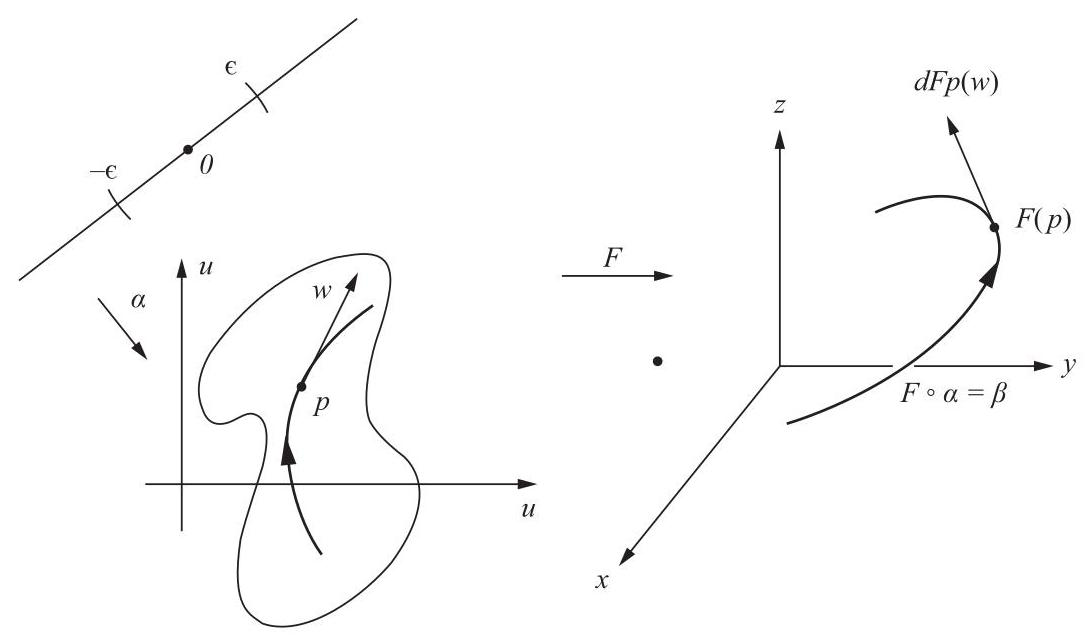
\includegraphics[max width=0.9\textwidth]{images/bo_d4b9jf3ef24c73e0334g_140_237_542_1091_637_0.jpg}
\end{center}
\hspace*{3em} 

图 A2-5

命题 7. 上述 \({\mathrm{{dF}}}_{\mathrm{p}}\) 的定义不依赖于通过 \(\mathrm{p}\) 且切向量为 \(\mathrm{w}\) 的曲线的选择，并且 \({\mathrm{{dF}}}_{\mathrm{p}}\) 实际上是一个线性映射.

证明. 为简化记号，我们处理 \(F : U \subset  {R}^{2} \rightarrow  {R}^{3}\) 的情况.设 \(\left( {u,v}\right)\) 为 \({R}^{2}\) 中的坐标，设 \(\left( {x,y,z}\right)\) 为 \({R}^{3}\) 中的坐标.设 \({e}_{1} = \left( {1,0}\right) ,{e}_{2} = \left( {0,1}\right)\) 为 \({R}^{2}\) 中的标准基，设 \({f}_{1} = \left( {1,0,0}\right)\) ， \({f}_{2} = \left( {0,1,0}\right) ,{f}_{3} = \left( {0,0,1}\right)\) 为 \({R}^{3}\) 中的标准基.则我们可以写出 \(\alpha \left( t\right)  = \left( {u\left( t\right) ,v\left( t\right) }\right) ,t \in  \left( {-\epsilon ,\epsilon }\right) ,\)

\[
{\alpha }^{\prime }\left( 0\right)  = w = {u}^{\prime }\left( 0\right) {e}_{1} + {v}^{\prime }\left( 0\right) {e}_{2},
\]

\(F\left( {u,v}\right)  = \left( {x\left( {u,v}\right) ,y\left( {u,v}\right) ,z\left( {u,v}\right) }\right)\) ，并且

\[
\beta \left( t\right)  = F \circ  \alpha \left( t\right)  = \left( {x\left( {u\left( t\right) ,v\left( t\right) }\right) ,y\left( {u\left( t\right) ,v\left( t\right) }\right) ,z\left( {u\left( t\right) ,v\left( t\right) }\right) }\right) .
\]

因此，利用链式法则并在 \(t = 0\) 处求导，我们得到

\[
{\beta }^{\prime }\left( 0\right)  = \left( {\frac{\partial x}{\partial u}\frac{du}{dt} + \frac{\partial x}{\partial v}\frac{dv}{dt}}\right) {f}_{1} + \left( {\frac{\partial y}{\partial u}\frac{du}{dt} + \frac{\partial y}{\partial v}\frac{dv}{dt}}\right) {f}_{2}
\]

\[
+ \left( {\frac{\partial z}{\partial u}\frac{du}{dt} + \frac{\partial z}{\partial v}\frac{dv}{dt}}\right) {f}_{3}
\]

\[
= \left( \begin{array}{ll} \frac{\partial x}{\partial u} & \frac{\partial x}{\partial v} \\  \frac{\partial y}{\partial u} & \frac{\partial y}{\partial v} \\  \frac{\partial z}{\partial u} & \frac{\partial z}{\partial v} \end{array}\right) \left( \begin{array}{l} \frac{du}{dt} \\  \frac{dv}{dt} \end{array}\right)  = d{F}_{p}\left( w\right) .
\]

这表明 \(d{F}_{p}\) 在 \({R}^{2}\) 和 \({R}^{3}\) 的标准基中由一个矩阵表示，该矩阵仅取决于 \(p\) 处 \(F\) 的分量函数 \(x,y,z\) 的偏导数.因此， \(d{F}_{p}\) 是一个线性映射，并且显然 \(d{F}_{p}\left( w\right)\) 不依赖于 \(\alpha\) 的选择.

读者将不难将此论证推广到更一般的情况.Q.E.D.

在 \({R}^{n}\) 和 \({R}^{m}\) 的标准基下的 \(d{F}_{p} : {R}^{n} \rightarrow  {R}^{m}\) 的矩阵，即矩阵 \(\left( {\partial {f}_{i}/\partial {x}_{j}}\right) ,i = 1,\ldots ,m,j = 1,\ldots ,n\) ，称为 \(F\) 在 \(p\) 处的雅可比矩阵.当 \(n = m\) 时，这是一个方阵，其行列式称为雅可比行列式；通常用它来表示

\[
\det \left( \frac{\partial {f}_{i}}{\partial {x}_{j}}\right)  = \frac{\partial \left( {{f}_{1},\ldots ,{f}_{n}}\right) }{\partial \left( {{x}_{1},\ldots ,{x}_{n}}\right) }.
\]

注记.关于微分的记号，文献中没有统一的规定.通常也称 \(d{F}_{p}\) 为 \(F\) 在 \(p\) 处的导数，并记为 \({F}^{\prime }\left( p\right)\) .

例 10. 设 \(F : {R}^{2} \rightarrow  {R}^{2}\) 由下式给出

\[
F\left( {x,y}\right)  = \left( {{x}^{2} - {y}^{2},{2xy}}\right) ,\;\left( {x,y}\right)  \in  {R}^{2}.
\]

容易看出 \(F\) 是可微的，其在 \(p = \left( {x,y}\right)\) 处的微分 \(d{F}_{p}\) 为

\[
d{F}_{p} = \left( \begin{matrix} {2x} &  - {2y} \\  {2y} & {2x} \end{matrix}\right) .
\]

例如， \(d{F}_{\left( 1,1\right) }\left( {2,3}\right)  = \left( {-2,{10}}\right)\) .

映射微分概念的一个优点是它允许我们用几何语言表达微积分的许多事实.例如，考虑以下情况:设 \(F : U \subset  {R}^{2} \rightarrow  {R}^{3},G : V \subset  {R}^{3} \rightarrow  {R}^{2}\) 是可微映射，其中 \(U\) 和 \(V\) 是开集，且 \(F\left( U\right)  \subset  V\) .我们约定以下坐标集，

\[
U \subset  {R}^{2}\xrightarrow[\left( u,v\right) ]{}V \subset  {R}^{3}\xrightarrow[\left( x,y,z\right) ]{}{R}^{2}
\]

并写出

\[
F\left( {u,v}\right)  = \left( {x\left( {u,v}\right) ,y\left( {u,v}\right) ,z\left( {u,v}\right) }\right) ,
\]

\[
G\left( {x,y,z}\right)  = \left( {\xi \left( {x,y,z}\right) ,\eta \left( {x,y,z}\right) }\right) .
\]

那么

\[
G \circ  F\left( {u,v}\right)  = \left( {\xi \left( {x\left( {u,v}\right) ,y\left( {u,v}\right) ,z\left( {u,v}\right) }\right) ,\eta \left( {x\left( {u,v}\right) ,y\left( {u,v}\right) ,z\left( {u,v}\right) }\right) }\right) ,
\]

根据链式法则，我们可以说 \(G \circ  F\) 是可微的，并计算其分量函数的偏导数.例如，

\[
\frac{\partial \xi }{\partial u} = \frac{\partial \xi }{\partial x}\frac{\partial x}{\partial u} + \frac{\partial \xi }{\partial y}\frac{\partial y}{\partial u} + \frac{\partial \xi }{\partial z}\frac{\partial z}{\partial u}.
\]

现在，表达上述情况的一个简单方法是使用以下一般事实.

命题 8(映射的链式法则).设 \(\mathrm{F} : \mathrm{U} \subset  {\mathbb{R}}^{N} \rightarrow  {\mathbb{R}}^{\mathrm{m}}\) 和 \(\mathrm{G} : \mathrm{V} \subset  {\mathbb{R}}^{\mathrm{m}} \rightarrow  {\mathbb{R}}^{\mathrm{k}}\) 是可微映射，其中 \(\mathrm{U}\) 和 \(\mathrm{V}\) 是开集，且 \(\mathrm{F}\left( \mathrm{U}\right)  \subset  \mathrm{V}\) .则 \(\mathrm{G} \circ  \mathrm{F} : \mathrm{U} \rightarrow  {\mathbb{R}}^{\mathrm{k}}\) 是一个可微映射，并且

\[
\mathrm{d}{\left( \mathrm{G} \circ  \mathrm{F}\right) }_{\mathrm{p}} = {\mathrm{{dG}}}_{\mathrm{F}\left( \mathrm{p}\right) } \circ  {\mathrm{{dF}}}_{\mathrm{p}},\;\mathrm{p} \in  \mathrm{U}.
\]

证明. \(G \circ  F\) 可微这一事实是函数链式法则的结果.现在，设 \({w}_{1} \in  {R}^{n}\) 给定，并考虑一条曲线 \(\alpha  : \left( {-{\epsilon }_{2},{\epsilon }_{2}}\right)  \rightarrow  U\) ，其中 \(\alpha \left( 0\right)  = p,{\alpha }^{\prime }\left( 0\right)  = {w}_{1}\) .设 \(d{F}_{p}\left( {w}_{1}\right)  = {w}_{2}\) 并注意到 \(d{G}_{F\left( p\right) }\left( {w}_{2}\right)  = {\left. \left( d/dt\right) \left( G \circ  F \circ  \alpha \right) \right| }_{t = 0}\) .则

\[
d{\left( G \circ  F\right) }_{p}\left( {w}_{1}\right)  = \frac{d}{dt}{\left( G \circ  F \circ  \alpha \right) }_{t = 0} = d{G}_{F\left( p\right) }\left( {w}_{2}\right)  = d{G}_{F\left( p\right) } \circ  d{F}_{p}\left( {w}_{1}\right) . \tag{Q.E.D.}
\]

请注意，对于我们之前考虑的特定情况，关系 \(d{\left( G \circ  F\right) }_{p} = d{G}_{F\left( p\right) } \circ  d{F}_{p}\) 等价于以下雅可比矩阵的乘积，

\[
\left( \begin{array}{ll} \frac{\partial \xi }{\partial u} & \frac{\partial \xi }{\partial v} \\  \frac{}{} & \\  \frac{\partial \eta }{\partial u} & \frac{\partial \eta }{\partial v} \end{array}\right)  = \left( \begin{array}{lll} \frac{\partial \xi }{\partial x} & \frac{\partial \xi }{\partial y} & \frac{\partial \xi }{\partial z} \\   & & \\  \frac{\partial \eta }{\partial x} & \frac{\partial \eta }{\partial y} & \frac{\partial \eta }{\partial z} \end{array}\right) \left( \begin{array}{ll} \frac{\partial x}{\partial u} & \frac{\partial x}{\partial v} \\  \frac{\partial y}{\partial u} & \frac{\partial y}{\partial v} \\  \frac{\partial z}{\partial u} & \frac{\partial z}{\partial v} \end{array}\right) ,
\]

包含所有偏导数的表达式 \(\partial \xi /\partial u,\partial \xi /\partial v,\partial \eta /\partial u\) ， \(\partial \eta /\partial v\) .因此，映射链式法则的简单表达式包含了其分量函数偏导数的丰富信息.

定义在开区间 \(\left( {a,b}\right)\) 上的可微函数 \(f : \left( {a,b}\right)  \subset  R \rightarrow  R\) 的一个重要性质是，如果在 \(\left( {a,b}\right)\) 上 \({f}^{\prime }\left( x\right)  \equiv  0\) ，则 \(f\) 在 \(\left( {a,b}\right)\) 上是常数.这可以推广到多变量可微函数，如下所示.

我们称开集 \(U \subset  {R}^{n}\) 是连通的，如果给定任意两点 \(p,q \in  U\) ，存在一个连续映射 \(\alpha  : \left\lbrack  {a,b}\right\rbrack   \rightarrow  U\) ，使得 \(\alpha \left( a\right)  = p\) 和 \(\alpha \left( b\right)  = q\) .这意味着 \(U\) 中的两点可以通过 \(U\) 中的连续曲线连接，或者说 \(U\) 由一个单一的“块”组成.

命题 9.设 \(\mathrm{f} : \mathrm{U} \subset  {\mathbb{R}}^{N} \rightarrow  \mathbb{R}\) 是定义在 \({\mathbb{R}}^{N}\) 的连通开子集 \(\mathrm{U}\) 上的可微函数.假设在每一点 \(\mathrm{p} \in  \mathrm{U}\) 处 \({\mathrm{{df}}}_{\mathrm{p}} : {\mathbb{R}}^{N} \rightarrow  \mathbb{R}\) 为零.则 \(\mathrm{f}\) 在 \(\mathrm{U}\) 上是常数.

证明.设 \(p \in  U\) ，令 \({B}_{\delta }\left( p\right)  \subset  U\) 为围绕 \(p\) 且包含在 \(U\) 中的一个开球.任意点 \(q \in  {B}_{\epsilon }\left( p\right)\) 可以通过“径向”线段 \(\beta  : \left\lbrack  {0,1}\right\rbrack   \rightarrow  U\) 连接到 \(p\) ，其中 \(\beta \left( t\right)  = {tq} + \left( {1 - t}\right) p,t \in  \left\lbrack  {0,1}\right\rbrack\) (图 A2-6).由于 \(U\) 是开的，我们可以将 \(\beta\) 扩展到 \(\left( {0 - \epsilon ,1 + \epsilon }\right)\) .现在， \(f \circ  \beta  : \left( {0 - \epsilon ,1 + \epsilon }\right)  \rightarrow  R\) 是定义在开区间上的一个函数，并且

\[
d{\left( f \circ  \beta \right) }_{t} = {\left( df \circ  d\beta \right) }_{t} = 0,
\]

因为 \({df} \equiv  0\) .因此，

\[
\frac{d}{dt}\left( {f \circ  \beta }\right)  = 0
\]

\begin{center}
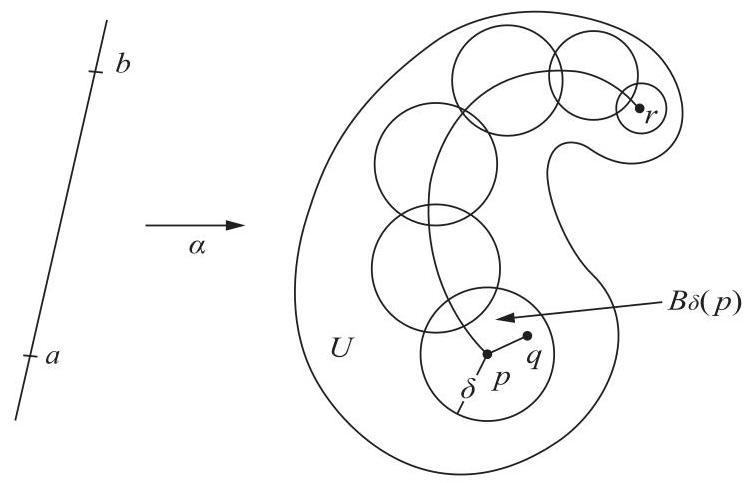
\includegraphics[max width=0.6\textwidth]{images/bo_d4b9jf3ef24c73e0334g_143_385_1558_751_483_0.jpg}
\end{center}
\hspace*{3em} 

图 A2-6

对于所有 \(t \in  \left( {0 - \epsilon ,1 + \epsilon }\right)\) ，因此 \(\left( {f \circ  \beta }\right)  =\) 是常数.这意味着 \(f\left( {\beta \left( 0\right) }\right)  = f\left( p\right)  = f\left( {\beta \left( 1\right) }\right)  = f\left( q\right)\) ；也就是说， \(f\) 在 \({B}_{\delta }\left( p\right)\) 上是常数.

因此，该命题在局部上得到了证明；也就是说， \(U\) 的每个点都有一个邻域，使得 \(f\) 在该邻域上是常数.请注意，到目前为止我们还没有使用 \(U\) 的连通性.我们现在需要它来证明这些常数都是相同的.

设 \(r\) 是 \(U\) 中的任意一点.由于 \(U\) 是连通的，存在一个连续曲线 \(\alpha  : \left\lbrack  {a,b}\right\rbrack   \rightarrow  U\) ，使得 \(\alpha \left( a\right)  = p,\alpha \left( b\right)  = r\) .函数 \(f \circ \; \alpha  : \left\lbrack  {a,b}\right\rbrack   \rightarrow  R\) 在 \(\left\lbrack  {a,b}\right\rbrack\) 上是连续的.根据证明的第一部分，对于每个 \(t \in  \left\lbrack  {a,b}\right\rbrack\) ，存在一个在 \(\left\lbrack  {a,b}\right\rbrack\) 中开的区间 \({I}_{t}\) ，使得 \(f \circ  \alpha\) 在 \({I}_{t}\) 上是常数.由于 \(\mathop{\bigcup }\limits_{t}{I}_{t} = \left\lbrack  {a,b}\right\rbrack\) ，我们可以应用 Heine-Borel 定理(命题 6).因此，我们可以选择有限个 \({I}_{t}\) 区间，记为 \({I}_{1},\ldots ,{I}_{k}\) 个，使得 \(\mathop{\bigcup }\limits_{i}{I}_{i} = \left\lbrack  {a,b}\right\rbrack  ,i = 1,\ldots ,k\) .我们可以假设，通过重新编号区间(如果需要)，使得两个连续的区间重叠.因此， \(f \circ  \alpha\) 在两个连续区间的并集上是常数.由此可知， \(f\) 在 \(\left\lbrack  {a,b}\right\rbrack\) 上是常数；即:

\[
f\left( {\alpha \left( a\right) }\right)  = f\left( p\right)  = f\left( {\alpha \left( b\right) }\right)  = f\left( r\right) .
\]

由于 \(r\) 是任意的， \(f\) 在 \(U\) 上是常数.Q.E.D.

微分学最重要的定理之一是所谓的反函数定理，用现在的记号表示如下.(回忆一下，线性映射 \(A\) 是一个同构，当且仅当 \(A\) 的矩阵是可逆的.)

反函数定理.设 \(\mathrm{F} : \mathrm{U} \subset  {\mathbb{R}}^{N} \rightarrow  {\mathbb{R}}^{N}\) 是一个可微映射，并假设在 \(\mathrm{p} \in  \mathrm{U}\) 处，微分 \({\mathrm{{dF}}}_{\mathrm{p}} : {\mathbb{R}}^{N} \rightarrow  {\mathbb{R}}^{N}\) 是一个同构.那么，在 \(\mathrm{U}\) 中存在 \(\mathrm{p}\) 的一个邻域 \(\mathrm{V}\) ，以及在 \({\mathbb{R}}^{N}\) 中存在 \(\mathrm{F}\left( \mathrm{p}\right)\) 的一个邻域 \(\mathrm{W}\) ，使得 \(\mathrm{F} : \mathrm{V} \rightarrow  \mathrm{W}\) 有一个可微的逆 \({F}^{-1} : W \rightarrow  V\) .

一个可微映射 \(F : V \subset  {R}^{n} \rightarrow  W \subset  {R}^{n}\) ，其中 \(V\) 和 \(W\) 是开集，称为从 \(V\) 到 \(W\) 的微分同胚，如果 \(F\) 有一个可微的逆.反函数定理断言，如果在点 \(p \in  U\) 处，微分 \(d{F}_{p}\) 是一个同构，那么 \(F\) 在 \(p\) 的一个邻域内是微分同胚.换句话说，关于 \(F\) 在某点处的微分的断言，意味着关于 \(F\) 在该点邻域的行为的类似断言.

本书将反复使用这个定理.例如，可以在 Buck 的《高等微积分》第 285 页找到证明.

例 11.设 \(F : {R}^{2} \rightarrow  {R}^{2}\) 由下式给出

\[
F\left( {x,y}\right)  = \left( {{e}^{x}\cos y,{e}^{x}\sin y}\right) ,\;\left( {x,y}\right)  \in  {R}^{2}.
\]

函数 \(F\) 的分量函数 \(u\left( {x,y}\right)  = {e}^{x}\cos y,v\left( {x,y}\right)  = \; {e}^{x}\sin y\) 具有所有阶的连续偏导数.因此， \(F\) 是可微的.

从几何上考察 \(F\) 如何变换 \({xy}\) 平面上的曲线是很有启发性的.例如，垂直线 \(x = {x}_{0}\) 被映射到半径为 \({e}^{{x}_{0}}\) 的圆 \(u = {e}^{{x}_{0}}\cos y,v = {e}^{{x}_{0}}\sin y\) 上，水平线 \(y = {y}_{0}\) 被映射到斜率为 tan \({y}_{0}\) 的半直线 \(u = {e}^{x}\cos {y}_{0},v = {e}^{x}\sin {y}_{0}\) 上.由此可知(图 A2-7)

\[
d{F}_{\left( {x}_{0},{y}_{0}\right) }\left( {1,0}\right)  = {\left. \frac{d}{dx}\left( {e}^{x}\cos {y}_{0},{e}^{x}\sin {y}_{0}\right) \right| }_{x = {x}_{0}}
\]

\[
= \left( {{e}^{{x}_{0}}\cos {y}_{0},{e}^{{x}_{0}}\sin {y}_{0}}\right) ,
\]

\[
d{F}_{\left( {x}_{0},{y}_{0}\right) }\left( {0,1}\right)  = {\left. \frac{d}{dy}\left( {e}^{{x}_{0}}\cos y,{e}^{{x}_{0}}\sin y\right) \right| }_{y = {y}_{0}}
\]

\[
= \left( {-{e}^{{x}_{0}}\sin {y}_{0},{e}^{{x}_{0}}\cos {y}_{0}}\right) .
\]

\begin{center}
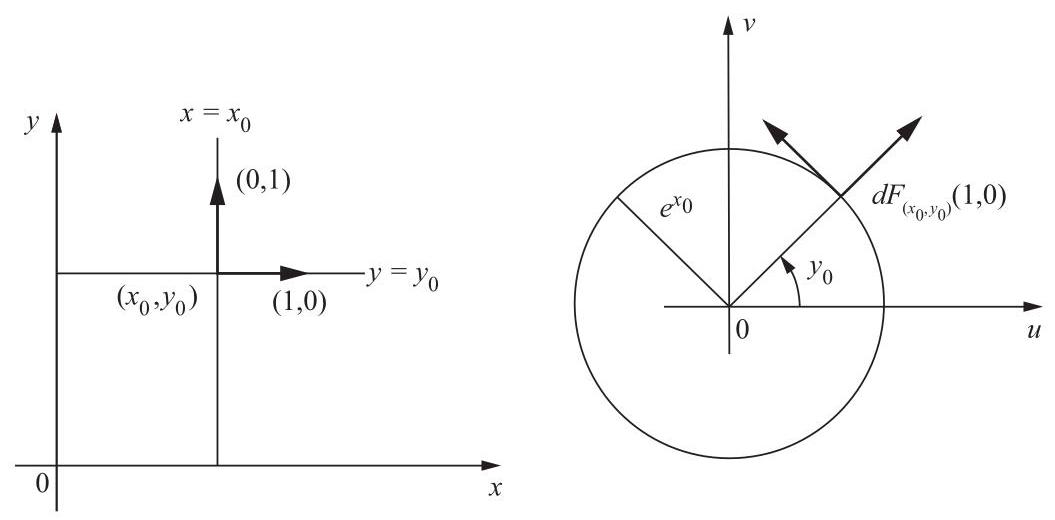
\includegraphics[max width=0.9\textwidth]{images/bo_d4b9jf3ef24c73e0334g_145_240_603_1055_520_0.jpg}
\end{center}
\hspace*{3em} 

图 A2-7

最容易通过计算 \(F\) 的雅可比矩阵来验证这一点，

\[
d{F}_{\left( x,y\right) } = \left( \begin{array}{ll} \frac{\partial u}{\partial x} & \frac{\partial u}{\partial y} \\  \frac{\partial v}{\partial x} & \frac{\partial v}{\partial y} \end{array}\right)  = \left( \begin{matrix} {e}^{x}\cos y &  - {e}^{x}\sin y \\   & \\  {e}^{x}\sin y & {e}^{x}\cos y \end{matrix}\right) ,
\]

并将其应用于 \(\left( {{x}_{0},{y}_{0}}\right)\) 处的向量 \(\left( {1,0}\right)\) 和 \(\left( {0,1}\right)\) .

我们注意到雅可比行列式 \(\det \left( {d{F}_{\left( x,y\right) }}\right)  = {e}^{x} \neq  0\) ，因此 \(d{F}_{p}\) 对于所有 \(p = \left( {x,y}\right)  \in  {R}^{2}\) 都是非奇异的(这从先前的几何考虑中也很清楚).因此，我们可以应用反函数定理得出结论， \(F\) 在局部是一个微分同胚.

观察到 \(F\left( {x,y}\right)  = F\left( {x,y + {2\pi }}\right)\) .因此， \(F\) 不是一对一的，并且没有全局逆.对于每一个 \(p \in  {R}^{2}\) ，逆函数定理给出了 \(p\) 的邻域 \(V\) 和 \(F\left( p\right)\) 的邻域 \(W\) ，使得限制 \(F : V \rightarrow  W\) 是一个微分同胚.在我们的例子中， \(V\) 可以取为条带 \(\{  - \infty  < x < \infty ,0 < \; y < {2\pi }\}\) ， \(W\) 可以取为 \({R}^{2} - \{ \left( {0,0}\right) \}\) .然而，正如例子所示，即使定理的条件在处处都满足，并且 \(F\) 的定义域非常简单， \(F\) 的全局逆也可能不存在.


4 曲面的内蕴几何

曲面

\section*{4-1. 引言}

在第 2 章中，我们介绍了曲面的第一基本形式 \(S\) ，并展示了如何使用它来计算曲面上简单的度量概念(长度、角度、面积等).关键在于，一旦知道了第一基本形式，就可以在不“离开”曲面的情况下进行此类计算.因此，这些概念被称为曲面的内蕴概念 \(S\) .

然而，第一基本形式的几何学并不局限于上面提到的简单概念.正如我们将在本章中看到的，曲面的许多重要局部性质只能用第一基本形式来表达.此类性质的研究被称为曲面的内蕴几何.本章致力于内蕴几何.

在第 4-2 节中，我们将定义等距的概念，它本质上精确地表达了两个曲面具有“相同”第一基本形式的直观想法.

在第 4-3 节中，我们将证明著名的 Gauss 公式，该公式将高斯曲率 \(K\) 表示为第一基本形式的系数及其导数的函数.这意味着 \(K\) 是一个内蕴概念，考虑到 \(K\) 是使用第二基本形式定义的，这是一个非常惊人的事实.

在第 4-4 节中，我们将开始系统地研究内蕴几何.事实证明，该主题可以通过曲面上向量场的协变导数概念来统一.这是平面上向量场通常导数的推广，并在整个章节中起着基本作用.

第 4-5 节致力于 Gauss-Bonnet 定理的局部和全局版本.这可能是本书最重要的定理.即使在短期课程中，也应该努力学习到第 4-5 节.

在第 4-6 节中，我们将定义指数映射，并使用它来引入两种特殊的坐标系，即法坐标和测地极坐标.

在第 4-7 节中，我们将讨论一些在前面各节中被搁置的关于测地线理论的精妙问题.例如，我们将证明，对于曲面 \(S\) 上的每一点 \(p\) ，都存在 \(S\) 中以 \(p\) 为中心的邻域，该邻域是其所有点的法域(法域的定义在第 4-6 节给出).这个结果及一个相关结果在第 5 章中使用；然而，在初读时，最好假定它们并省略第 4-7 节.我们还将证明凸域的存在性，但这在本书的其他地方均不使用.

\section*{4-2. 等距映射；共形映射}

第 2-5 节的例 1 和例 2 显示了一个有趣的特点.尽管圆柱面和平面是不同的曲面，但它们的 الأول 基础形式是“相等”的(至少在我们考虑的坐标邻域中是如此).这意味着，就内在度量问题(长度、角度、面积)而言，平面和圆柱面在局部上的表现是相同的.(这是直观上清晰的，因为通过沿一条母线切割圆柱面，我们可以将其展开成平面的一部分.)在本章中，我们将看到许多与正则曲面相关的其他重要概念仅取决于 الأول 基础形式，应归类为内在概念.因此，我们有必要精确地阐述两个正则曲面具有相等的 الأول 基础形式的含义.

\(S\) 和 \(\bar{S}\) 始终表示正则曲面.

定义 1. 映射 \(\varphi  : S \rightarrow  \overline{S}\) 是一个等距映射，如果对于所有 \(\mathrm{p} \in  S\) 和所有点对 \({\mathrm{w}}_{1},{\mathrm{w}}_{2} \in  {\mathrm{T}}_{\mathrm{p}}\left( S\right)\) ，都有

\[
{\left\langle  {\mathrm{w}}_{1},{\mathrm{w}}_{2}\right\rangle  }_{\mathrm{p}} = {\left\langle  \mathrm{d}{\varphi }_{\mathrm{p}}\left( {\mathrm{w}}_{1}\right) ,\mathrm{d}{\varphi }_{\mathrm{p}}\left( {\mathrm{w}}_{2}\right) \right\rangle  }_{\varphi \left( \mathrm{p}\right) }.
\]

则称曲面 \(S\) 和 \(\overline{S}\) 是等距的.

换句话说，映射 \(\varphi\) 是一个等距映射，如果其微分 \({d\varphi }\) 保持内积.由此可知，若 \({d\varphi }\) 是一个等距映射，则

\[
{I}_{p}\left( w\right)  = \langle w,w{\rangle }_{p} = {\left\langle  d{\varphi }_{p}\left( w\right) ,d{\varphi }_{p}\left( w\right) \right\rangle  }_{\varphi \left( p\right) } = {I}_{\varphi \left( p\right) }\left( {d{\varphi }_{p}\left( w\right) }\right)
\]

对于所有 \(w \in  {T}_{p}\left( S\right)\) .反之，如果一个映射 \(\varphi\) 保持 الأول 基础形式，即

\[
{I}_{p}\left( w\right)  = {I}_{\varphi \left( p\right) }\left( {d{\varphi }_{p}\left( w\right) }\right) \;\text{ for all }w \in  {T}_{p}\left( S\right) ,
\]

则

\[
2\left\langle  {{w}_{1},{w}_{2}}\right\rangle   = {I}_{p}\left( {{w}_{1} + {w}_{2}}\right)  - {I}_{p}\left( {w}_{1}\right)  - {I}_{p}\left( {w}_{2}\right)
\]

\[
= {I}_{\varphi \left( p\right) }\left( {d{\varphi }_{p}\left( {{w}_{1} + {w}_{2}}\right) }\right)  - {I}_{\varphi \left( p\right) }\left( {d{\varphi }_{p}\left( {w}_{1}\right) }\right)  - {I}_{\varphi \left( p\right) }\left( {d{\varphi }_{p}\left( {w}_{2}\right) }\right)
\]

\[
= 2\left\langle  {d{\varphi }_{p}\left( {w}_{1}\right) ,d{\varphi }_{p}\left( {w}_{2}\right) }\right\rangle  ,
\]

因此， \(\varphi\) 是一个等距映射.

定义 2. 若存在 \(\varphi \left( \mathrm{p}\right)  \in  \overline{S}\) 的一个邻域 \(\overline{\mathrm{V}}\) 使得 \(\varphi  : \mathrm{V} \rightarrow  \overline{\mathrm{V}}\) 为等距映射，则从 \(\mathrm{p} \in  S\) 的邻域 \(\mathrm{V}\) 出发的映射 \(\varphi  : \mathrm{V} \rightarrow  \overline{S}\) 在 \(\mathrm{p}\) 处为局部等距映射.若在每一点 \(\mathrm{p} \in  S\) 处都存在到 \(\overline{S}\) 的局部等距映射，则称曲面 \(S\) 局部等距于 \(S\) .若 \(S\) 局部等距于 \(S\) 且 \(S\) 局部等距于 \(S\) ，则称 \(S\) 和 \(S\) 局部等距.

显然，如果 \(\varphi  : S \rightarrow  \bar{S}\) 是一个映射且对于每个 \(p \in  S\) 都是局部等距映射，那么 \(\varphi\) 就是一个(全局)等距映射.然而，可能出现两个曲面局部等距但(全局)不等距的情况，如下例所示.

令 \(\varphi\) 为圆柱体在坐标邻域 \(\overline{\mathbf{x}}\left( U\right)\) 到平面 \(\mathbf{x}\left( {R}^{2}\right)\) 的映射，其中圆柱体由 2-5 节例 2 定义，平面由 2-5 节例 1 定义，映射由 \(\varphi  = \mathbf{x} \circ  {\overline{\mathbf{x}}}^{-1}\) 定义(我们已将圆柱体参数化中的 \(\mathbf{x}\) 改为 \(\overline{\mathbf{x}}\) ).那么 \(\varphi\) 是一个局部等距映射.事实上，圆柱体上某点 \(p \in  \overline{\mathbf{x}}\left( U\right)\) 处的切向量 \(w\) ，是曲线 \(\overline{\mathbf{x}}\left( {u\left( t\right) ,v\left( t\right) }\right)\) 的切向量，其中 \(\left( {u\left( t\right) ,v\left( t\right) }\right)\) 是 \(U \subset  {R}^{2}\) 中的一条曲线.因此， \(w\) 可以写成

\[
w = {\overline{\mathbf{x}}}_{u}{u}^{\prime } + {\overline{\mathbf{x}}}_{v}{v}^{\prime }.
\]

另一方面， \({d\varphi }\left( w\right)\) 是曲线的切向量

\[
\varphi \left( {\overline{\mathbf{x}}\left( {u\left( t\right) ,v\left( t\right) }\right) }\right)  = \mathbf{x}\left( {u\left( t\right) ,v\left( t\right) }\right) .
\]

因此， \({d\varphi }\left( w\right)  = {\mathbf{x}}_{u}{u}^{\prime } + {\mathbf{x}}_{v}{v}^{\prime }\) .由于 \(E = \bar{E},F = \bar{F},G = \bar{G}\) ，我们得到

\[
{I}_{p}\left( w\right)  = \bar{E}{\left( {u}^{\prime }\right) }^{2} + 2\bar{F}{u}^{\prime }{v}^{\prime } + \bar{G}{\left( {v}^{\prime }\right) }^{2}
\]

\[
= E{\left( {u}^{\prime }\right) }^{2} + {2F}{u}^{\prime }{v}^{\prime } + G{\left( {v}^{\prime }\right) }^{2} = {I}_{\varphi \left( p\right) }\left( {d{\varphi }_{p}\left( w\right) }\right) ,
\]

正如我们所声称的.由此可知，圆柱体 \({x}^{2} + {y}^{2} = 1\) 在局部上与平面等距.

该等距映射不能扩展到整个圆柱体，因为圆柱体甚至与平面不全等价.对后一个断言的严格证明将使我们离题太远，但以下直观论证可以提供证明思路.平面中的任何简单闭合曲线都可以连续地收缩成一点而不离开平面(图 4-1).这样的性质在全等映射下肯定会被保留.但是圆柱体的一个平行圈(图 4-1)不具备这个性质，这就与平面和圆柱体之间存在全等映射的假设相矛盾.

\begin{center}
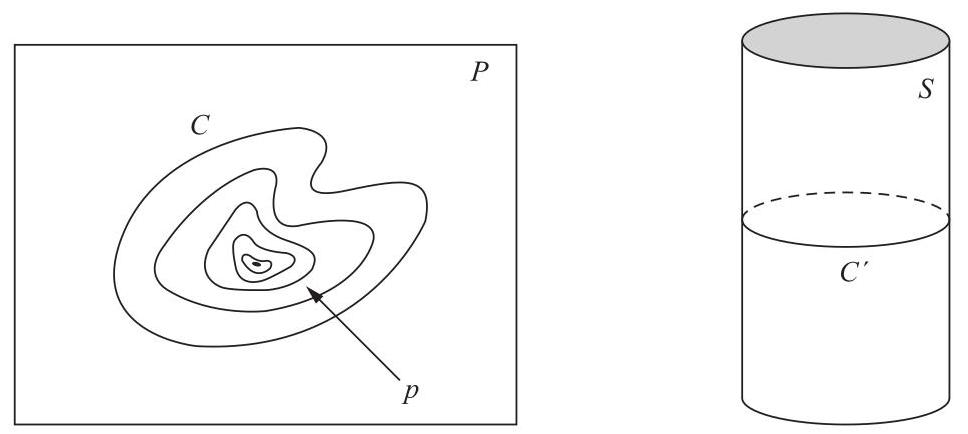
\includegraphics[max width=0.8\textwidth]{images/bo_d4b9jf3ef24c73e0334g_234_303_193_968_434_0.jpg}
\end{center}
\hspace*{3em} 

图 4-1. \(C \subset  P\) 可以连续地收缩成 \(p\) 而不离开 \(P\) .对于 \({C}^{\prime } \subset  S\) 则不然.

在给出更多例子之前，我们将推广上述论证，以获得一个关于局部坐标下局部等距的判据.

命题 1. 假设存在参数化 \(\mathbf{x} : \mathrm{U} \rightarrow  S\) 和 \(\overline{\mathbf{x}} : \mathrm{U} \rightarrow  \overline{S}\) ，使得在 \(\mathrm{U}\) 中有 \(\mathrm{E} = \overline{\mathrm{E}},\mathrm{F} = \overline{\mathrm{F}},\mathrm{G} = \overline{\mathrm{G}}\) .那么映射 \(\varphi  = \; \overline{\mathbf{x}} \circ  {\mathbf{x}}^{-1} : \mathbf{x}\left( \mathrm{U}\right)  \rightarrow  \overline{S}\) 是一个局部等距映射.

证明. 令 \(p \in  \mathbf{x}\left( U\right)\) 和 \(w \in  {T}_{p}\left( S\right)\) .那么 \(w\) 是曲线 \(\mathbf{x}\left( {\alpha \left( t\right) }\right)\) 在 \(t = 0\) 处的切向量，其中 \(\alpha \left( t\right)  = \left( {u\left( t\right) ,v\left( t\right) }\right)\) 是 \(U\) 中的一条曲线；因此， \(w\) 可以写成 \(\left( {t = 0}\right)\)

\[
w = {\mathbf{x}}_{u}{u}^{\prime } + {\mathbf{x}}_{v}{v}^{\prime }
\]

根据定义，向量 \(d{\varphi }_{p}\left( w\right)\) 是曲线 \(\overline{\mathbf{x}} \circ  {\mathbf{x}}^{-1} \circ \; \mathbf{x}\left( {\alpha \left( t\right) }\right)\) 的切向量，即曲线 \(\overline{\mathbf{x}}\left( {\alpha \left( t\right) }\right)\) 在 \(t = 0\) 处的切向量(图 4-2).因此，

\[
d{\varphi }_{p}\left( w\right)  = {\overline{\mathbf{x}}}_{u}{u}^{\prime } + {\overline{\mathbf{x}}}_{v}{v}^{\prime }.
\]

因为

\[
{I}_{p}\left( w\right)  = E{\left( {u}^{\prime }\right) }^{2} + {2F}{u}^{\prime }{v}^{\prime } + G{\left( {v}^{\prime }\right) }^{2},
\]

\[
{I}_{\varphi \left( p\right) }\left( {d{\varphi }_{p}\left( w\right) }\right)  = \bar{E}{\left( {u}^{\prime }\right) }^{2} + 2\bar{F}{u}^{\prime }{v}^{\prime } + \bar{G}{\left( {v}^{\prime }\right) }^{2},
\]

我们得出结论，对于所有 \(p \in  \mathbf{x}\left( U\right)\) 和所有 \(w \in  {T}_{p}\left( S\right)\) ，都有 \({I}_{p}\left( w\right)  = {I}_{\varphi \left( p\right) }\left( {d{\varphi }_{p}\left( w\right) }\right)\) ；因此， \(\varphi\) 是一个局部等距映射.证毕.

\begin{center}
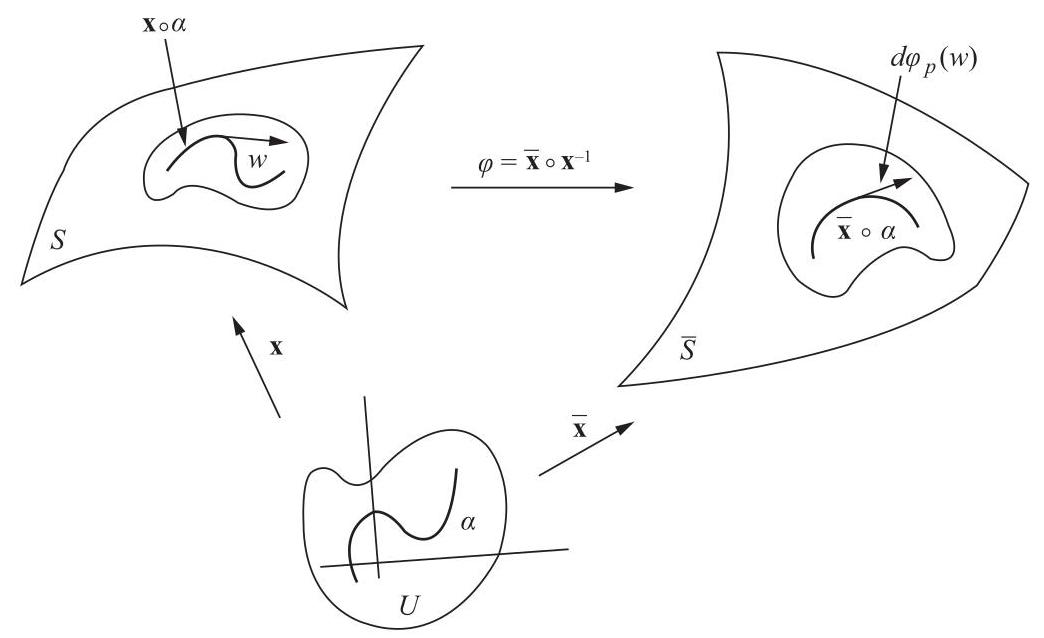
\includegraphics[max width=0.9\textwidth]{images/bo_d4b9jf3ef24c73e0334g_235_242_198_1044_638_0.jpg}
\end{center}
\hspace*{3em} 

图 4-2

例 2. 令 \(S\) 为一个旋转曲面，令

\[
\mathbf{x}\left( {u,v}\right)  = \left( {f\left( v\right) \cos u,f\left( v\right) \sin u,g\left( v\right) }\right) ,
\]

\[
a < v < b,\;0 < u < {2\pi },\;f\left( v\right)  > 0,
\]

为 \(S\) 的一个参数化(参见例 4，第 2-3 节).在参数化 \(\mathbf{x}\) 下， \(S\) 的第一基本形式系数由下式给出:

\[
E = {\left( f\left( v\right) \right) }^{2},\;F = 0,\;G = {\left( {f}^{\prime }\left( v\right) \right) }^{2} + {\left( {g}^{\prime }\left( v\right) \right) }^{2}.
\]

特别地，悬链线旋转曲面，

\[
x = a\cosh v,\;z = {av},\; - \infty  < v < \infty ,
\]

具有以下参数化:

\[
\mathbf{x}\left( {u,v}\right)  = \left( {a\cosh v\cos u,a\cosh v\sin u,{av}}\right) ,
\]

\[
0 < u < {2\pi },\; - \infty  < v < \infty ,
\]

相对于它，第一基本形式的系数为

\[
E = {a}^{2}{\cosh }^{2}v,\;F = 0,\;G = {a}^{2}\left( {1 + {\sinh }^{2}v}\right)  = {a}^{2}{\cosh }^{2}v.
\]

这个旋转曲面称为链面(见图 4-3).我们将证明链面在局部上与例 3，第 2-5 节中的螺旋面是等距的.

螺旋面的参数化由下式给出:

\[
\overline{\mathbf{x}}\left( {\bar{u},\bar{v}}\right)  = \left( {\bar{v}\cos \bar{u},\bar{v}\sin \bar{u},a\bar{u}}\right) ,\;0 < \bar{u} < {2\pi }, - \infty  < \bar{v} < \infty .
\]

\begin{center}
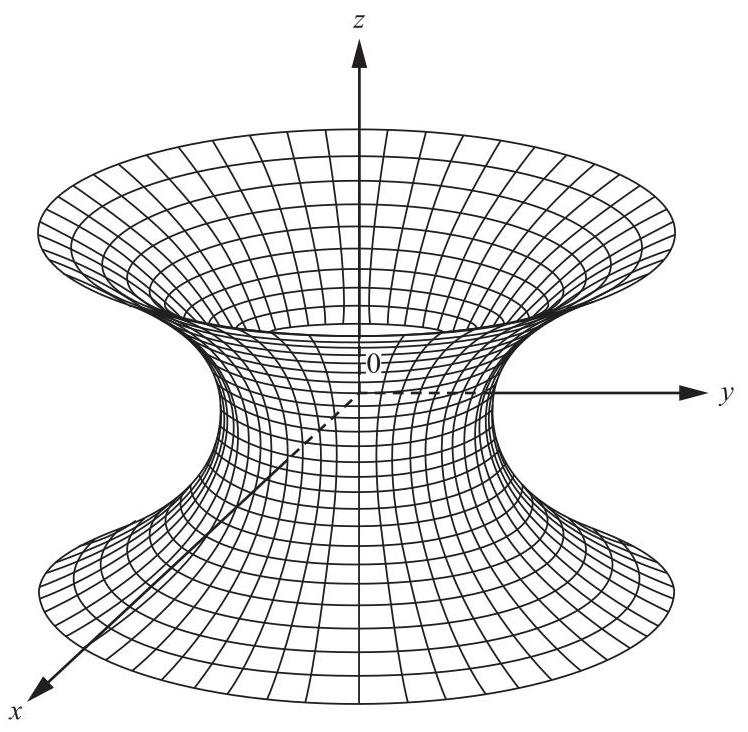
\includegraphics[max width=0.6\textwidth]{images/bo_d4b9jf3ef24c73e0334g_236_413_201_748_732_0.jpg}
\end{center}
\hspace*{3em} 

图 4-3. 链面.

我们进行以下参数变换:

\[
\bar{u} = u,\;\bar{v} = a\sinh v,\;0 < u < {2\pi }, - \infty  < v < \infty ,
\]

这是可能的，因为该映射显然是一一对应的，并且雅可比行列式

\[
\frac{\partial \left( {\bar{u},\bar{v}}\right) }{\partial \left( {u,v}\right) } = a\cosh v
\]

处处非零.因此，螺旋面的一种新参数化是

\[
\overline{\mathbf{x}}\left( {u,v}\right)  = \left( {a\sinh v\cos u,a\sinh v\sin u,{au}}\right) ,
\]

相对于它，第一基本形式的系数由下式给出:

\[
E = {a}^{2}{\cosh }^{2}v,\;F = 0,\;G = {a}^{2}{\cosh }^{2}v.
\]

利用命题1，我们得出悬链面和螺旋面是局部等距的.

图4-4给出了等距映射如何操作的几何概念；它将螺旋面的一“圈”(对应于 \(0 < u < {2\pi }\) 的坐标邻域)映射到悬链面减去一条经线.

注1. 螺旋面与悬链面之间的等距映射已在第3章极小曲面的背景下出现；参见第3-5节的练习14.

例3. 我们将证明单叶锥(除去顶点)

\[
z =  + k\sqrt{{x}^{2} + {y}^{2}},\;\left( {x,y}\right)  \neq  \left( {0,0}\right) ,
\]

与平面局部等距.其思想是证明一个锥面减去一条母线可以“滚动”到一个平面片上.

\begin{center}
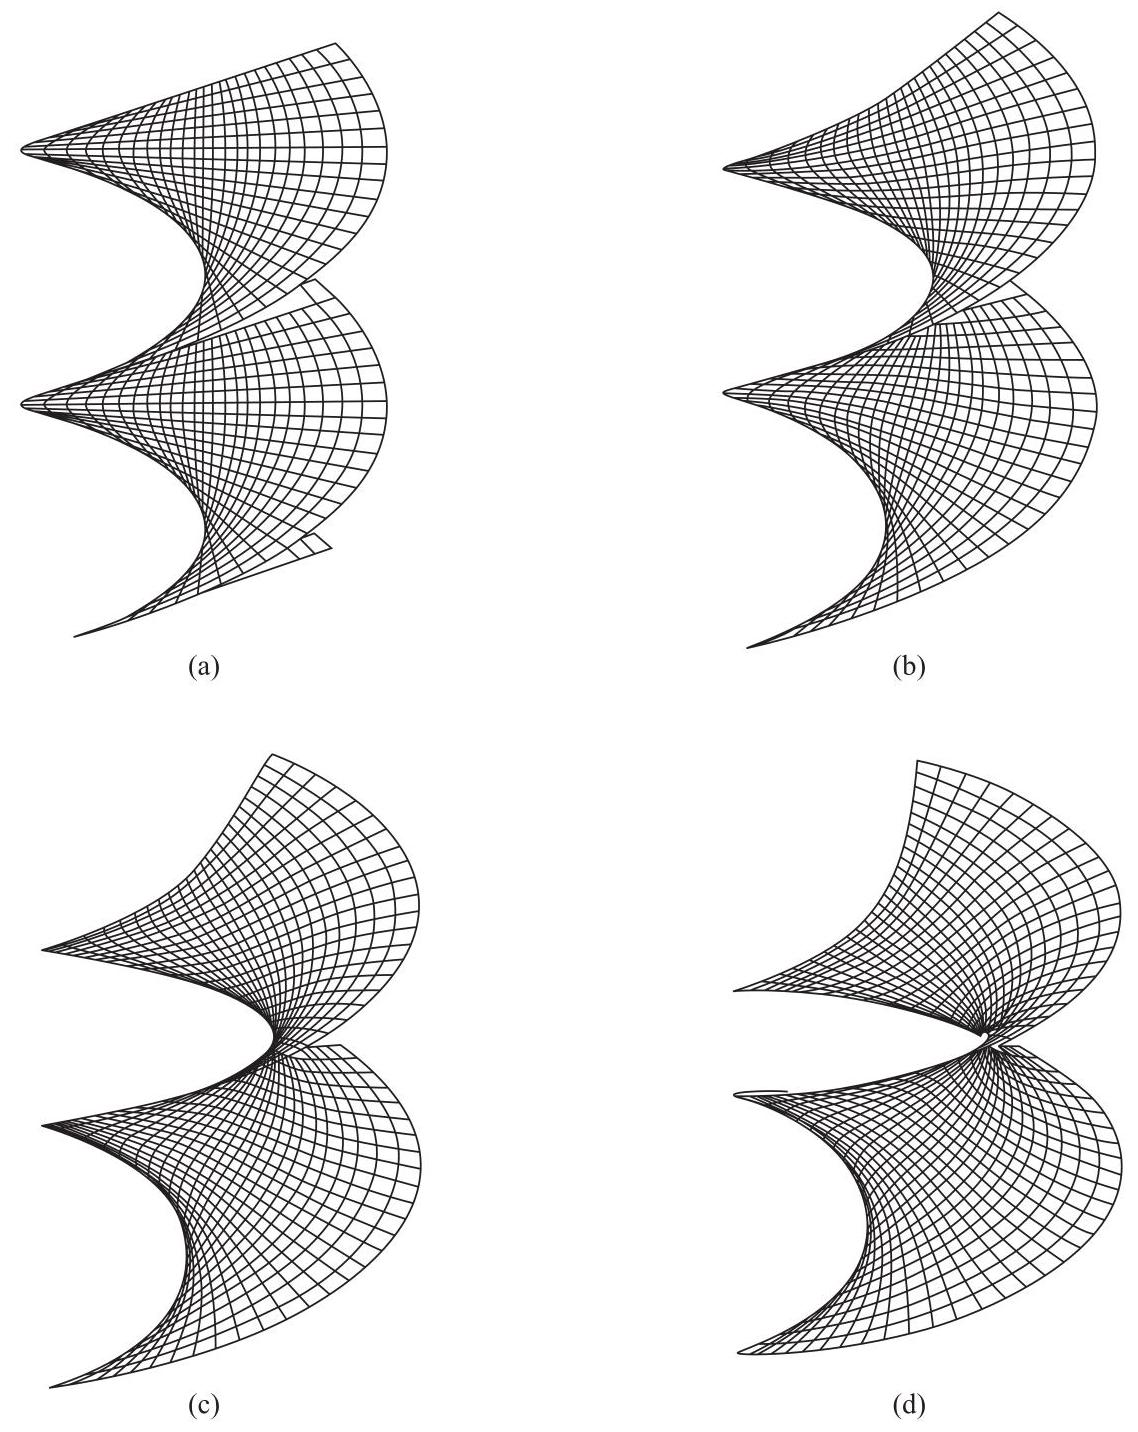
\includegraphics[max width=1.0\textwidth]{images/bo_d4b9jf3ef24c73e0334g_237_195_570_1138_1432_0.jpg}
\end{center}
\hspace*{3em} 

图4-4. 螺旋面到悬链面的等距变形.(a) 相1.(b) 相2.(c) 相3.(d) 相4.

\begin{center}
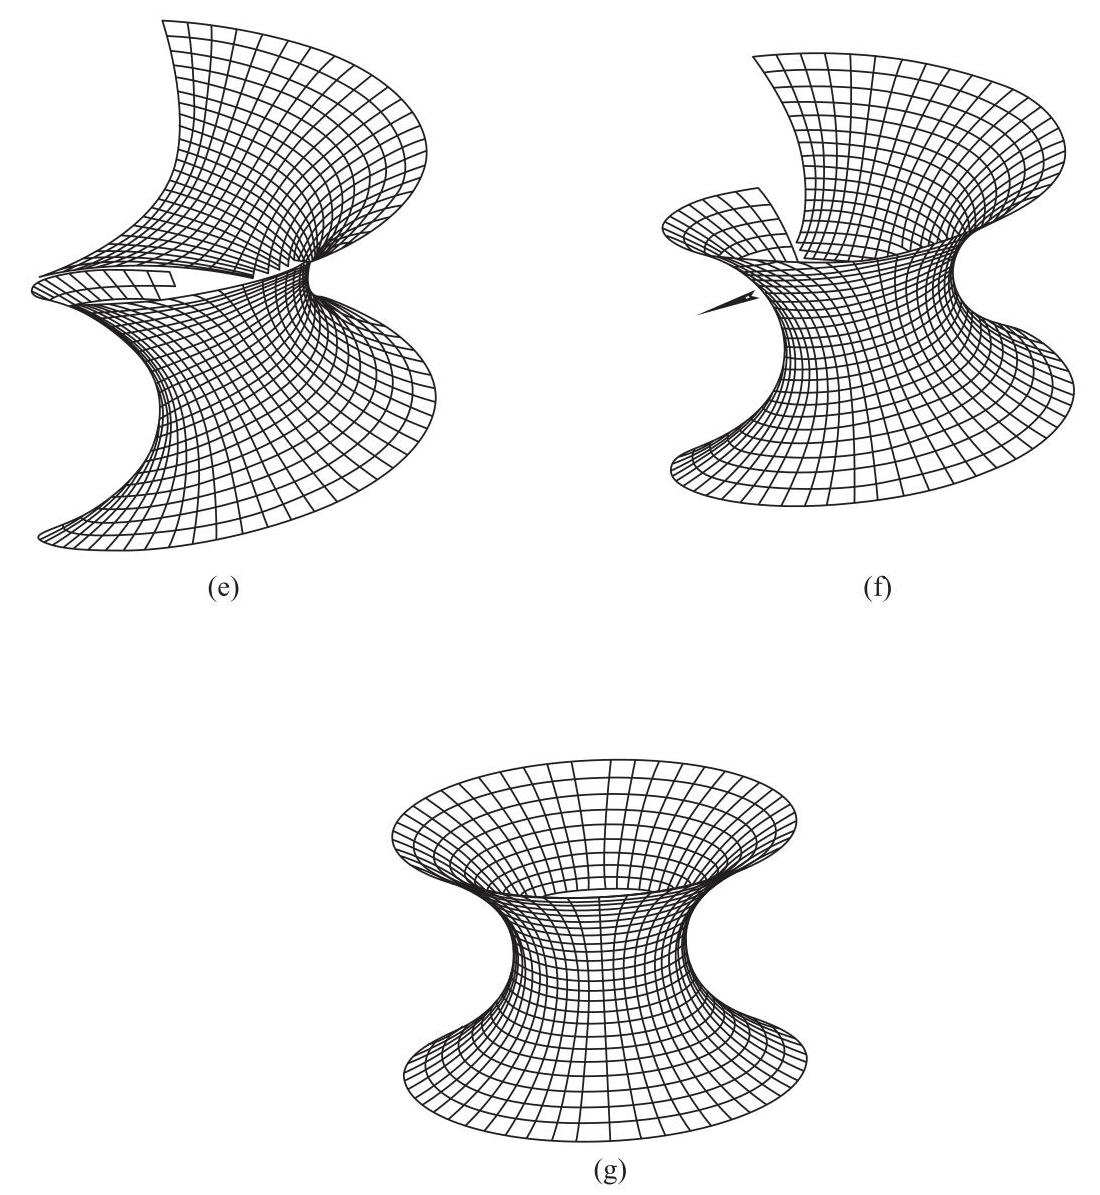
\includegraphics[max width=0.9\textwidth]{images/bo_d4b9jf3ef24c73e0334g_238_230_186_1100_1195_0.jpg}
\end{center}
\hspace*{3em} 

图4-4. (e) 相5.(f) 相6.(g) 相7.

设 \(U \subset  {R}^{2}\) 为在极坐标 \(\left( {\rho ,\theta }\right)\) 下给出的开集

\[
0 < \rho  < \infty ,\;0 < \theta  < {2\pi }\sin \alpha ,
\]

其中 \({2\alpha }\left( {0 < {2\alpha } < \pi }\right)\) 是锥顶角(即，其中余切 \(\alpha  = k)\) )，设 \(f : U \rightarrow  {R}^{3}\) 为映射(图4-5)

\[
f\left( {\rho ,\theta }\right)  = \left( {\rho \sin \alpha \cos \left( \frac{\theta }{\sin \alpha }\right) ,\rho \sin \alpha \sin \left( \frac{\theta }{\sin \alpha }\right) ,\rho \cos \alpha }\right) .
\]

显然 \(f\left( U\right)\) 包含在锥面中，因为

\[
k\sqrt{{x}^{2} + {y}^{2}} = \operatorname{cotan}\alpha \sqrt{{\rho }^{2}{\sin }^{2}\alpha } = \rho \cos \alpha  = z.
\]

\begin{center}
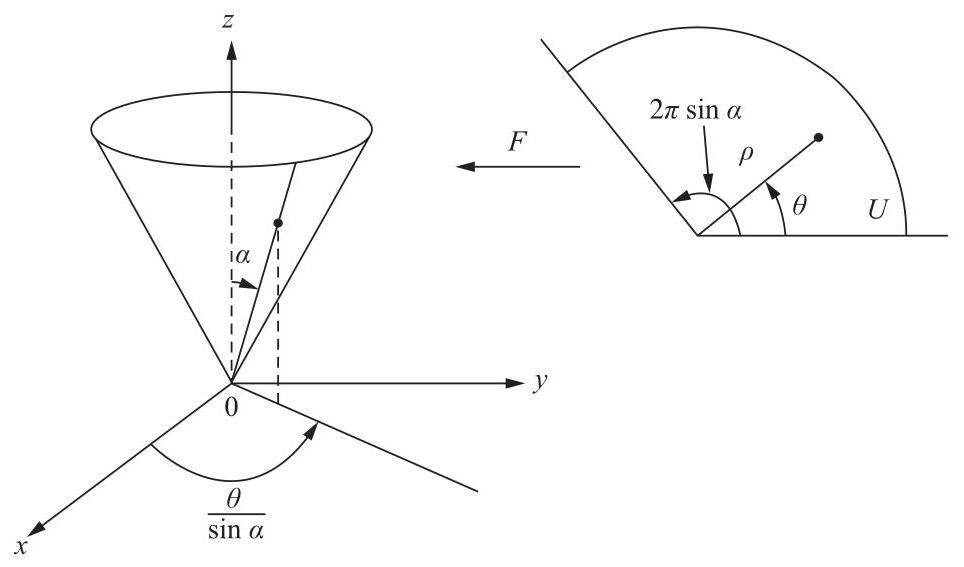
\includegraphics[max width=0.8\textwidth]{images/bo_d4b9jf3ef24c73e0334g_239_286_200_964_567_0.jpg}
\end{center}
\hspace*{3em} 

图4-5

此外，当 \(\theta\) 描述区间 \(\left( {0,{2\pi }\sin \alpha }\right) ,\theta /\sin \alpha\) 时， \(\left( {0,{2\pi }\sin \alpha }\right) ,\theta /\sin \alpha\) 描述区间 \(\left( {0,{2\pi }}\right)\) .因此，除了母线 \(\theta  = 0\) 之外的所有锥面点都被 \(f\left( U\right)\) 覆盖.

容易验证 \(f\) 和 \({df}\) 在 \(U\) 中是一一对应的；因此， \(f\) 是从 \(U\) 到除去一条母线的锥面的一个微分同胚.

我们现在将证明 \(f\) 是一个等距映射.事实上， \(U\) 可以被看作一个正则曲面，由以下参数化给出

\[
\overline{\mathbf{x}}\left( {\rho ,\theta }\right)  = \left( {\rho \cos \theta ,\rho \sin \theta ,0}\right) ,\;0 < \rho  < \infty ,0 < \theta  < {2\pi }\sin \alpha .
\]

在此参数化下， \(U\) 的第一个基本形式系数为

\[
\bar{E} = 1,\;\bar{F} = 0,\;\bar{G} = {\rho }^{2}.
\]

另一方面，在参数化 \(F \circ  \overline{\mathbf{x}}\) 下，锥面的第一个基本形式系数为

\[
E = 1,\;F = 0,\;G = {\rho }^{2}.
\]

根据命题 1，我们得出 \(F\) 是一个局部等距映射，正如我们所期望的.

注 2. 事实上，我们可以仅使用第一基本形式来计算曲面上 \(S\) 的曲线长度，这允许我们引入 \(S\) 中点之间的“内禀”距离的概念.粗略地说，我们定义 \(S\) 中两点 \(p\) 和 \(q\) 之间的(内禀)距离 \(d\left( {p,q}\right)\) 为连接 \(p\) 和 \(q\) 的 \(S\) 上曲线长度的下确界.(我们将在第 5-3 节中更详细地讨论这一点.)这个距离显然大于或等于 \(p\) 到 \(q\) 作为 \({R}^{3}\) 中的点的距离 \(\parallel p - q\parallel\) (图 4-6).我们将在练习 3 中证明，距离 \(d\) 在等距映射下是不变的；也就是说，如果 \(\varphi  : S \rightarrow  \bar{S}\) 是一个等距映射，那么 \(d\left( {p,q}\right)  = d\left( {\varphi \left( p\right) ,\varphi \left( q\right) }\right) ,p,q \in  S.\)

\begin{center}
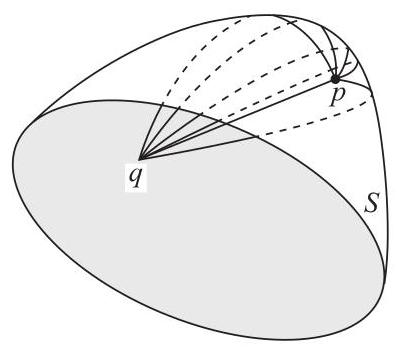
\includegraphics[max width=0.3\textwidth]{images/bo_d4b9jf3ef24c73e0334g_240_197_191_397_352_0.jpg}
\end{center}
\hspace*{3em} 

图 4-6

等距映射的概念是正则曲面度量性质的自然等价概念.正如可微同胚曲面在可微性观点下是等价的，等距曲面在度量观点下也是等价的.

在曲面研究中，可以定义进一步的等价类型.从我们的观点来看，微分同胚和等距映射是最重要的.然而，在处理与复变量的解析函数相关的问题时，引入共形等价是很重要的，我们现在将简要讨论这一点.

定义 3. 一个微分同胚 \(\varphi  : S \rightarrow  \overline{S}\) 被称为共形映射，如果对于所有 \(\mathrm{p} \in  S\) 和所有 \({\mathrm{v}}_{1},{\mathrm{v}}_{2} \in  {\mathrm{T}}_{\mathrm{p}}\left( S\right)\) ，我们有

\[
\left\langle  {\mathrm{d}{\varphi }_{\mathrm{p}}\left( {\mathrm{v}}_{1}\right) ,\mathrm{d}{\varphi }_{\mathrm{p}}\left( {\mathrm{v}}_{2}\right) }\right\rangle   = {\lambda }^{2}\left( \mathrm{p}\right) {\left\langle  {\mathrm{v}}_{1},{\mathrm{v}}_{2}\right\rangle  }_{\mathrm{p}}\text{ , }
\]

其中 \({\lambda }^{2}\) 是 \(S\) 上一个处处非零的可微函数；曲面 \(S\) 和 \(\mathrm{\bar{S}}\) 则被称为共形.一个映射 \(\varphi  : \mathrm{V} \rightarrow  \mathrm{\bar{S}}\) 从 \(\mathrm{p} \in  S\) 的一个邻域 \(\mathrm{V}\) 到 \(S\) ，如果存在 \(\varphi \left( \mathrm{p}\right)\) 的一个邻域 \(\mathrm{V}\) 使得 \(\varphi  : \mathrm{V} \rightarrow  \overline{\mathrm{V}}\) 是一个共形映射，则称其为 \(\mathrm{p}\) 处的局部共形映射.如果对于每个 \(\mathrm{p} \in  S\) ，都存在一个 \(\mathrm{p}\) 处的局部共形映射，则称曲面 \(S\) 与 \(\overline{S}\) 是局部共形的.

上述定义的几何意义是，角度(但不一定是长度)被共形映射所保持.事实上，设 \(\alpha  : I \rightarrow  S\) 和 \(\beta  : I \rightarrow  S\) 是 \(S\) 中相交于，比如说， \(t = 0\) 的两条曲线.它们在 \(t = 0\) 处的夹角 \(\theta\) 由下式给出:

\[
\cos \theta  = \frac{\left\langle  {\alpha }^{\prime },{\beta }^{\prime }\right\rangle  }{\left| {\alpha }^{\prime }\right| \left| {\beta }^{\prime }\right| },\;0 \leq  \theta  \leq  \pi .
\]

一个共形映射 \(\varphi  : S \rightarrow  \bar{S}\) 将这些曲线映射为曲线 \(\varphi  \circ  \alpha  : I \rightarrow  \bar{S}\) 、 \(\varphi  \circ  \beta  : I \rightarrow  \bar{S}\) ，它们在 \(t = 0\) 处相交，形成一个夹角 \(\overline{\theta }\) ，由下式给出:

\[
\cos \overline{\theta } = \frac{\left\langle  d\varphi \left( {\alpha }^{\prime }\right) ,d\varphi \left( {\beta }^{\prime }\right) \right\rangle  }{\left| {{d\varphi }\left( {\alpha }^{\prime }\right) }\right| \left| {{d\varphi }\left( {\beta }^{\prime }\right) }\right| } = \frac{{\lambda }^{2}\left\langle  {{\alpha }^{\prime },{\beta }^{\prime }}\right\rangle  }{{\lambda }^{2}\left| {\alpha }^{\prime }\right| \left| {\beta }^{\prime }\right| } = \cos \theta ,
\]

正如我们所声称的.不难证明这个性质表征了局部共形映射(练习 14).

以下命题是保形映射的命题1的类似物，其证明也留作练习.

命题 2. 设 \(x : \mathrm{U} \rightarrow  S\) 和 \(\overline{\mathbf{x}} : \mathrm{U} \rightarrow  \overline{S}\) 是参数化，使得在 \(\mathrm{U}\) 中有 \(\mathrm{E} = {\lambda }^{2}\overline{\mathrm{E}},\mathrm{F} = {\lambda }^{2}\overline{\mathrm{F}},\mathrm{G} = {\lambda }^{2}\overline{\mathrm{G}}\) ，其中 \({\lambda }^{2}\) 是 \(\mathrm{U}\) 中的一个处处非零的可微函数.则映射 \(\varphi  = \overline{\mathbf{x}} \circ  {\mathbf{x}}^{-1} : \mathbf{x}\left( \mathrm{U}\right)  \rightarrow  \overline{S}\) 是一个局部共形映射.

局部保形性很容易被看作是一种传递关系；也就是说，如果 \({S}_{1}\) 与 \({S}_{2}\) 局部保形，并且 \({S}_{2}\) 与 \({S}_{3}\) 局部保形，那么 \({S}_{1}\) 与 \({S}_{3}\) 局部保形.

保形映射最重要的性质由以下定理给出，我们不在此证明.

定理. 任何两个正则曲面都是局部保形的.

证明基于以下可能性:可以对正则曲面任何点的邻域进行参数化，使得第一基本形式的系数为

\[
E = {\lambda }^{2}\left( {u,v}\right)  > 0,\;F = 0,\;G = {\lambda }^{2}\left( {u,v}\right) .
\]

这样的坐标系称为等温坐标系.一旦假设存在正则曲面 \(S\) 的等温坐标系， \(S\) 显然与平面局部保形，并且通过复合与任何其他曲面局部保形.

任何正则曲面上存在等温坐标系这一证明很微妙，在此不予讨论.感兴趣的读者可以参考 L. Bers, Riemann Surfaces, New York University, Institute of Mathematical Sciences, New York, 1957-1958, pp. 15-35.

注3. 等温参数化已在第3章的极小曲面部分出现过；参见命题2和第3-5节的练习13.

\exerciseline

1. 设 \(F : U \subset  {R}^{2} \rightarrow  {R}^{3}\) 由下式给出

\[
F\left( {u,v}\right)  = \left( {u\sin \alpha \cos v,u\sin \alpha \sin v,u\cos \alpha }\right) ,
\]

\[
\left( {u,v}\right)  \in  U = \left\{  {\left( {u,v}\right)  \in  {R}^{2};u > 0}\right\}  ,\;\alpha  = \text{ const. }
\]

a. 证明 \(F\) 是 \(U\) 到以原点为顶点、 \({2\alpha }\) 为顶角角的圆锥 \(C\) 的局部微分同胚.

b. \(F\) 是局部等距映射吗？

2. 证明命题1的以下“逆命题”:设 \(\varphi  : S \rightarrow  \bar{S}\) 是一个等距映射， \(\mathbf{x} : U \rightarrow  S\) 是 \(p \in  S\) 处的一个参数化；则 \(\overline{\mathbf{x}} = \varphi  \circ  \mathbf{x}\) 是 \(\varphi \left( p\right)\) 处的一个参数化，并且 \(E = \bar{E},F = \bar{F},G = \bar{G}\) .

*3. 证明一个微分同胚 \(\varphi  : S \rightarrow  \bar{S}\) 是一个等距映射当且仅当 \(S\) 中任何参数化曲线的弧长等于 \(\varphi\) 的像曲线的弧长.

4. 使用立体投影(参见第2-2节练习16)证明球体与平面局部保形.

5. 设 \({\alpha }_{1} : I \rightarrow  {R}^{3},{\alpha }_{2} : I \rightarrow  {R}^{3}\) 为正则参数化曲线，其中参数为弧长.假设 \({\alpha }_{1}\) 的曲率 \({k}_{1}\) 和 \({\alpha }_{2}\) 的曲率 \({k}_{2}\) 满足 \({k}_{1}\left( s\right)  = {k}_{2}\left( s\right)  \neq  0,s \in  I\) .设

\[
{\mathbf{x}}_{1}\left( {s,v}\right)  = {\alpha }_{1}\left( s\right)  + v{\alpha }_{1}^{\prime }\left( s\right)
\]

\[
{\mathbf{x}}_{2}\left( {s,v}\right)  = {\alpha }_{2}\left( s\right)  + v{\alpha }_{2}^{\prime }\left( s\right)
\]

为它们的(正则)切面(参见例5，第2-3节)，设 \(V\) 为 \(\left( {{s}_{0},{v}_{0}}\right)\) 的一个邻域，使得 \({\mathbf{x}}_{1}\left( V\right)  \subset  {R}^{3},{\mathbf{x}}_{2}\left( V\right)  \subset  {R}^{3}\) 为正则曲面(参见命题2，第2-3节).证明 \({\mathbf{x}}_{1} \circ  {\mathbf{x}}_{2}^{-1} : {\mathbf{x}}_{2}\left( V\right)  \rightarrow  {\mathbf{x}}_{1}\left( V\right)\) 是等距映射.

*6. 设 \(\alpha  : I \rightarrow  {R}^{3}\) 为具有 \(k\left( t\right)  \neq  0,t \in  I\) 的正则参数化曲线.设 \(\mathbf{x}\left( {t,v}\right)\) 为其切面.证明，对于每个 \(\left( {{t}_{0},{v}_{0}}\right)  \in  I \times \; \left( {R-\{ 0\} }\right)\) ，存在 \(\left( {{t}_{0},{v}_{0}}\right)\) 的一个邻域 \(V\) ，使得 \(\mathbf{x}\left( V\right)\) 与平面上的一个开集等距(因此，切面局部等距于平面).

7. 设 \(V\) 和 \(W\) 为( \(n\) 维)向量空间，其内积分别记为 \(\langle\) ， \(\rangle {andletF} : V \rightarrow  W\) 为线性映射.证明以下条件等价:

a. 对所有 \({v}_{1},{v}_{2} \in  V\) ，有 \(\left\langle  {F\left( {v}_{1}\right) ,F\left( {v}_{2}\right) }\right\rangle   = \left\langle  {{v}_{1},{v}_{2}}\right\rangle\) .

b. 对所有 \(v \in  V\) ，有 \(\left| {F\left( v\right) }\right|  = \left| v\right|\) .

c. 如果 \(V\) 中存在一个标准正交基 \(\left\{  {{v}_{1},\ldots ,{v}_{n}}\right\}\) ，则 \(W\) 中存在一个标准正交基 \(\left\{  {F\left( {v}_{1}\right) ,\ldots ,F\left( {v}_{n}\right) }\right\}\) .

d. 存在 \(V\) 中的一个标准正交基 \(\left\{  {{v}_{1},\ldots ,{v}_{n}}\right\}\) ，使得 \(W\) 中存在一个标准正交基 \(\left\{  {F\left( {v}_{1}\right) ,\ldots ,F\left( {v}_{n}\right) }\right\}\) .

如果满足这些条件中的任何一个，则称 \(F\) 为从 \(V\) 到 \(W\) 的线性等距映射.(当 \(W = V\) 时，线性等距映射常被称为正交变换.)

*8. 设 \(G : {R}^{3} \rightarrow  {R}^{3}\) 为一个映射，使得

\[
\left| {G\left( p\right)  - G\left( q\right) }\right|  = \left| {p - q}\right| \;\text{ for all }p,q \in  {R}^{3}
\]

(即， \(G\) 是一个保距映射).证明存在 \({p}_{0} \in  {R}^{3}\) 和向量空间 \({R}^{3}\) 的线性等距映射(参见练习 7) \(F\) ，使得

\[
G\left( p\right)  = F\left( p\right)  + {p}_{0}\;\text{ for all }p \in  {R}^{3}.
\]

9. 设 \({S}_{1},{S}_{2}\) 和 \({S}_{3}\) 是正则曲面.证明:

a. 如果 \(\varphi  : {S}_{1} \rightarrow  {S}_{2}\) 是等距映射，则 \({\varphi }^{-1} : {S}_{2} \rightarrow  {S}_{1}\) 也是等距映射.

b. 如果 \(\varphi  : {S}_{1} \rightarrow  {S}_{2},\psi  : {S}_{2} \rightarrow  {S}_{3}\) 是等距映射，则 \(\psi  \circ  \varphi  : {S}_{1} \rightarrow  {S}_{3}\) 是等距映射.

这表明正则曲面 \(S\) 的等距映射自然构成一个群，称为 \(S\) 的等距映射群.

10. 设 \(S\) 是一个旋转曲面.证明绕其轴线的旋转是 \(S\) 的等距映射.

11. a. 设 \(S \subset  {R}^{3}\) 是一个正则曲面，令 \(F : {R}^{3} \rightarrow  {R}^{3}\) 是 \({R}^{3}\) 的一个保距微分同胚(参见练习 8)，使得 \(F\left( S\right)  \subset  S\) .证明 \(F\) 在 \(S\) 上的限制是 \(S\) 的一个等距映射.

b. 利用 a 部分证明单位球面 \({x}^{2} + {y}^{2} + {z}^{2} = 1\) 的等距映射群(参见练习 10)包含 \({R}^{3}\) 的正交线性变换群(实际上它们相等；参见第 4-4 节练习 23).

c. 举例说明存在 \(\varphi  : {S}_{1} \rightarrow  {S}_{2}\) 的等距映射不能扩展为 \(F : {R}^{3} \rightarrow  {R}^{3}\) 的保距映射.

*12. 设 \(C = \left\{  {\left( {x,y,z}\right)  \in  {R}^{3};{x}^{2} + {y}^{2} = 1}\right\}\) 是一个圆柱体.构造一个等距映射 \(\varphi  : C \rightarrow  C\) ，使得 \(\varphi\) 的不动点集，即集合 \(\{ p \in  C;\varphi \left( p\right)  = p\}\) ，恰好包含两个点.

13. 设 \(V\) 和 \(W\) 是具有内积 \(\langle\) 、 \(\rangle .\) 的 \(\left( {n\text{ -dimensional }}\right)\) 向量空间.设 \(G : V \rightarrow  W\) 是一个线性映射.证明以下条件等价:

a. 存在一个实常数 \(\lambda  \neq  0\) 使得

\[
\left\langle  {G\left( {v}_{1}\right) ,G\left( {v}_{2}\right) }\right\rangle   = {\lambda }^{2}\left\langle  {{v}_{1},{v}_{2}}\right\rangle  \;\text{ for all }{v}_{1},{v}_{2} \in  V.
\]

b. 存在一个实常数 \(\lambda  > 0\) 使得

\[
\left| {G\left( v\right) }\right|  = \lambda \left| v\right| \;\text{ for all }v \in  V.
\]

c. 存在 \(V\) 的一个标准正交基 \(\left\{  {{v}_{1},\ldots ,{v}_{n}}\right\}\) ，使得 \(\left\{  {G\left( {v}_{1}\right) ,\ldots ,G\left( {v}_{n}\right) }\right\}\) 是 \(W\) 的一个正交基，并且向量 \(G\left( {v}_{i}\right) ,i = 1,\ldots ,n\) 具有相同的(非零)长度.

如果满足这些条件中的任何一个，则称 \(G\) 为线性保角映射(或相似变换).

14. 当对于任意 \(p \in  {S}_{1}\) 和任意一对 \({v}_{1},{v}_{2} \in  {T}_{p}\left( {S}_{1}\right)\) 都有时，我们称可微映射 \(\varphi  : {S}_{1} \rightarrow  {S}_{2}\) 保角.

\[
\cos \left( {{v}_{1},{v}_{2}}\right)  = \cos \left( {d{\varphi }_{p}\left( {v}_{1}\right) ,d{\varphi }_{p}\left( {v}_{2}\right) }\right) .
\]

证明 \(\varphi\) 是局部共形映射当且仅当它保角.

15. 令 \(\varphi  : {R}^{2} \rightarrow  {R}^{2}\) 由 \(\varphi \left( {x,y}\right)  = \left( {u\left( {x,y}\right) ,v\left( {x,y}\right) }\right)\) 给出，其中 \(u\) 和 \(v\) 是满足柯西-黎曼方程的可微函数.

\[
{u}_{x} = {v}_{y},\;{u}_{y} =  - {v}_{x}.
\]

证明 \(\varphi\) 是从 \({R}^{2} - Q\) 到 \({R}^{2}\) 的局部保形映射，其中 \(Q = \left\{  {\left( {x,y}\right)  \in  {R}^{2};{u}_{x}^{2} + {u}_{y}^{2} = 0}\right\}  .\)

16. 令 \(\mathbf{x} : U \subset  {R}^{2} \rightarrow  {R}^{3}\) ，其中

\[
U = \left\{  {\left( {\theta ,\varphi }\right)  \in  {R}^{2};0 < \theta  < \pi ,0 < \varphi  < {2\pi }}\right\}  ,
\]

\[
\mathbf{x}\left( {\theta ,\varphi }\right)  = \left( {\sin \theta \cos \varphi ,\sin \theta \sin \varphi ,\cos \theta }\right) ,
\]

是单位球面 \({S}^{2}\) 的参数化.令

\[
\log \tan \frac{1}{2}\theta  = u,\;\varphi  = v,
\]

并证明坐标邻域 \(\mathbf{x}\left( U\right)  = V\) 的新参数化可以由

\[
\mathbf{y}\left( {u,v}\right)  = \left( {\operatorname{sech}u\cos v,\operatorname{sech}u\sin v,\tanh u}\right) .
\]

证明在参数化 \(\mathbf{y}\) 中，第一基本形式的系数是

\[
E = G = {\operatorname{sech}}^{2}u,\;F = 0.
\]

因此， \({\mathbf{y}}^{-1} : V \subset  {S}^{2} \rightarrow  {R}^{2}\) 是一个共形映射，它将 \({S}^{2}\) 的子午线和纬线映射到平面上的直线.这称为墨卡托投影.

*17. 考虑单位球面上的一个三角形，其边由等角线段组成(即与子午线成恒定角度的曲线；参见第 2-5 节的示例 4)，并且不包含极点.证明这样的三角形的内角和是 \(\pi\) .

18. 如果一个区域 \(R \subset  S\) 的面积等于 \(\varphi \left( R\right)\) 的面积，则称微分同胚 \(\varphi  : S \rightarrow  \bar{S}\) 是保面积的.证明如果 \(\varphi\) 是保面积且共形的，则 \(\varphi\) 是等距映射.

19. 令 \({S}^{2} = \left\{  {\left( {x,y,z}\right)  \in  {R}^{3};{x}^{2} + {y}^{2} + {z}^{2} = 1}\right\}\) 为单位球面， \(C = \; \left\{  {\left( {x,y,z}\right)  \in  {R}^{3};{x}^{2} + {y}^{2} = 1}\right\}\) 为外切圆柱面.令

\[
\varphi  : {S}^{2} - \{ \left( {0,0,1}\right)  \cup  \left( {0,0, - 1}\right) \}  = M \rightarrow  C
\]

为如下定义的映射.对于每个 \(p \in  M\) ，通过 \(p\) 且垂直于 \({0z}\) 的直线在 \({0z}\) 上相交于点 \(q\) .令 \(l\) 为从 \(q\) 开始并包含 \(p\) 的半直线(图 4-7).根据定义， \(\varphi \left( p\right)  = C \cap  l\) .

\begin{center}
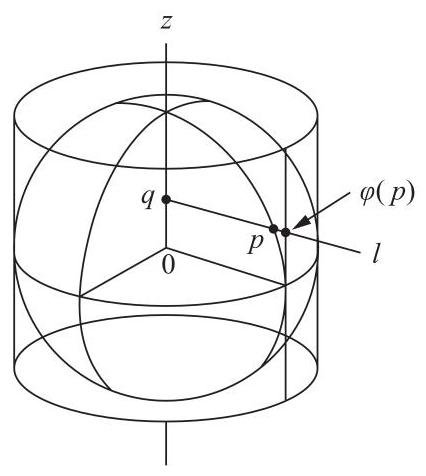
\includegraphics[max width=0.3\textwidth]{images/bo_d4b9jf3ef24c73e0334g_245_179_390_426_476_0.jpg}
\end{center}
\hspace*{3em} 

图 4-7

证明 \(\varphi\) 是一个保面积微分同胚.

20. 令 \(\mathbf{x} : U \subset  {R}^{2} \rightarrow  S\) 为旋转曲面 \(S\) 的参数化:

\[
\mathbf{x}\left( {u,v}\right)  = \left( {f\left( v\right) \cos u,f\left( v\right) \sin u,g\left( v\right) }\right) ,\;f\left( v\right)  > 0,
\]

\[
U = \left\{  {\left( {u,v}\right)  \in  {R}^{2};0 < u < {2\pi },a < v < b}\right\}  .
\]

a. 证明由下式给出的映射 \(\varphi  : U \rightarrow  {R}^{2}\)

\[
\varphi \left( {u,v}\right)  = \left( {u,\int \frac{\sqrt{{\left( {f}^{\prime }\left( v\right) \right) }^{2} + {\left( {g}^{\prime }\left( v\right) \right) }^{2}}}{f\left( v\right) }{dv}}\right)
\]

是一个局部微分同胚.

b. 利用 a 部分证明旋转曲面 \(S\) 在局部上与平面共形，使得每个局部共形映射 \(\theta\) : \(V \subset  S \rightarrow  {R}^{2}\) 将邻域 \(V\) 的平行线和经线映射到 \(\theta \left( V\right)  \subset  {R}^{2}\) 中的一组正交直线系统.(注意，这推广了练习 16 的墨卡托投影.)

c. 证明由下式给出的映射 \(\psi  : U \rightarrow  {R}^{2}\)

\[
\psi \left( {u,v}\right)  = \left( {u,\int f\left( v\right) \sqrt{{\left( {f}^{\prime }\left( v\right) \right) }^{2} + {\left( {g}^{\prime }\left( v\right) \right) }^{2}}{dv}}\right)
\]

是一个局部微分同胚.

d. 利用 \(c\) 部分证明，对于旋转曲面 \(S\) 的每一点 \(p\) ，都存在一个邻域 \(V \subset  S\) 和一个将 \(V\) 映射到平面的保面积映射 \(\overline{\theta } : V \rightarrow  {R}^{2}\) .

\section*{4-3. 高斯定理与相容性方程}

第 3 章的性质是从研究切平面在某点邻域的变化中获得的.类比曲线，我们将为曲面上的每一点分配一个三面体(费雷三面体的类似物)，并研究其向量的导数.

如常， \(S\) 表示一个正则、可定向、定向的曲面.令 \(\mathbf{x} : U \subset  {R}^{2} \rightarrow  S\) 为 \(S\) 方向的参数化.可以为 \(\mathbf{x}\left( U\right)\) 的每一点分配一个由向量 \({\mathbf{x}}_{u},{\mathbf{x}}_{v}\) 和 \(N\) 给出的自然三面体.本节将研究这个三面体.

通过在基 \(\left\{  {{\mathbf{x}}_{u},{\mathbf{x}}_{v},N}\right\}\) 中表示向量 \({\mathbf{x}}_{u},{\mathbf{x}}_{v}\) 和 \(N\) 的导数，我们得到

\[
{\mathbf{x}}_{uu} = {\mathbf{\Gamma }}_{11}^{1}{\mathbf{x}}_{u} + {\mathbf{\Gamma }}_{11}^{2}{\mathbf{x}}_{v} + {L}_{1}N
\]

\[
{\mathbf{x}}_{uv} = {\mathbf{\Gamma }}_{12}^{1}{\mathbf{x}}_{u} + {\mathbf{\Gamma }}_{12}^{2}{\mathbf{x}}_{v} + {L}_{2}N
\]

\[
{\mathbf{x}}_{vu} = {\mathbf{\Gamma }}_{21}^{1}{\mathbf{x}}_{u} + {\mathbf{\Gamma }}_{21}^{2}{\mathbf{x}}_{v} + {\bar{L}}_{2}N \tag{1}
\]

\[
{\mathbf{x}}_{vv} = {\mathbf{\Gamma }}_{22}^{1}{\mathbf{x}}_{u} + {\mathbf{\Gamma }}_{22}^{2}{\mathbf{x}}_{v} + {L}_{3}N
\]

\[
{N}_{u} = {a}_{11}{\mathbf{x}}_{u} + {a}_{21}{\mathbf{x}}_{v},
\]

\[
{N}_{v} = {a}_{12}{\mathbf{x}}_{u} + {a}_{22}{\mathbf{x}}_{v},
\]

其中 \({a}_{ij},i,j = 1,2\) 在第 3 章中获得，其他系数待定.系数 \({\mathbf{\Gamma }}_{ij}^{k},i,j,k = 1,2\) 称为 \(S\) 在参数化 \(\mathbf{x}\) 下的克里斯托费尔符号.由于 \({\mathbf{x}}_{uv} = {\mathbf{x}}_{vu}\) ，我们得出 \({\mathbf{\Gamma }}_{12}^{1} = {\mathbf{\Gamma }}_{21}^{1}\) 和 \({\mathbf{\Gamma }}_{12}^{2} = {\mathbf{\Gamma }}_{21}^{2}\) ；也就是说，克里斯托费尔符号相对于下指标是对称的.

通过将 (1) 中的前四个关系与 \(N\) 进行内积，我们立即得到 \({L}_{1} = e,{L}_{2} = {\bar{L}}_{2} = f,{L}_{3} = g\) ，其中 \(e,f,g\) 是 \(S\) 的第二基本形式的系数.

为了确定克里斯托费尔符号，我们取前四个关系与 \({\mathbf{x}}_{u}\) 和 \({\mathbf{x}}_{v}\) 的内积，得到系统

\[
\left\{  \begin{array}{l} {\mathbf{\Gamma }}_{11}^{1}E + {\mathbf{\Gamma }}_{11}^{2}F = \left\langle  {{\mathbf{x}}_{uu},{\mathbf{x}}_{u}}\right\rangle   = \frac{1}{2}{E}_{u}, \\  {\mathbf{\Gamma }}_{11}^{1}F + {\mathbf{\Gamma }}_{11}^{2}G = \left\langle  {{\mathbf{x}}_{uu},{\mathbf{x}}_{v}}\right\rangle   = {F}_{u} - \frac{1}{2}{E}_{v}, \end{array}\right.
\]

\[
\left\{  \begin{array}{l} {\mathbf{\Gamma }}_{12}^{1}E + {\mathbf{\Gamma }}_{12}^{2}F = \left\langle  {{\mathbf{x}}_{uv},{\mathbf{x}}_{u}}\right\rangle   = \frac{1}{2}{E}_{v}, \\  {\mathbf{\Gamma }}_{12}^{1}F + {\mathbf{\Gamma }}_{12}^{2}G = \left\langle  {{\mathbf{x}}_{uv},{\mathbf{x}}_{v}}\right\rangle   = \frac{1}{2}{G}_{u}, \end{array}\right. \tag{2}
\]

\[
\left\{  \begin{array}{l} {\mathbf{\Gamma }}_{22}^{1}E + {\mathbf{\Gamma }}_{22}^{2}F = \left\langle  {{\mathbf{x}}_{vv},{\mathbf{x}}_{u}}\right\rangle   = {F}_{v} - \frac{1}{2}{G}_{u}, \\  {\mathbf{\Gamma }}_{22}^{1}F + {\mathbf{\Gamma }}_{22}^{2}G = \left\langle  {{\mathbf{x}}_{vv},{\mathbf{x}}_{v}}\right\rangle   = \frac{1}{2}{G}_{v}. \end{array}\right.
\]

请注意，上述方程已分为三对方程，对于每一对方程，系统的行列式为 \({EG} - {F}^{2} \neq  0\) .

因此，可以解出上述系统并用第一基本形式的系数 E、F、G 及其导数来计算克里斯托费尔符号.我们不会得到 \({\mathbf{\Gamma }}_{ij}^{k}\) 的显式表达式，因为在每种特定情况下，使用方程组 (2) 更为容易.(参见下面的示例 1.)然而，我们能够解出方程组 (2) 的以下推论非常重要:用克里斯托费尔符号表示的所有几何概念和性质在等距变换下是不变的.

示例 1. 我们将计算由(参见第 2-3 节，示例 4)参数化的旋转曲面的克里斯托费尔符号.

\[
\mathbf{x}\left( {u,v}\right)  = \{ f\left( v\right) \cos u,f\left( v\right) \sin u,g\left( v\right) ),\;f\left( v\right)  \neq  0.
\]

因为

\[
E = {\left( f\left( v\right) \right) }^{2},\;F = 0,\;G = {\left\{  {f}^{\prime }\left( v\right) \right) }^{2} + {\left( {g}^{\prime }\left( v\right) \right) }^{2},
\]

我们得到

\[
{E}_{u} = 0,\;{E}_{v} = {2f}{f}^{\prime },
\]

\[
{F}_{u} = {F}_{v} = 0,\;{G}_{u} = 0,
\]

\[
{G}_{v} = 2\left( {{f}^{\prime }{f}^{\prime \prime } + {g}^{\prime }{g}^{\prime \prime }}\right) ,
\]

其中撇号表示相对于 \(v\) 的导数.方程组 (2) 的前两个方程给出

\[
{\Gamma }_{11}^{1} = 0,\;{\Gamma }_{11}^{2} =  - \frac{f{f}^{\prime }}{{\left( {f}^{\prime }\right) }^{2} + {\left( {g}^{\prime }\right) }^{2}}.
\]

接下来，方程组 (2) 的第二对方程给出

\[
{\Gamma }_{12}^{1} = \frac{f{f}^{\prime }}{{f}^{2}},\;{\Gamma }_{12}^{2} = 0.
\]

最后，从方程组 (2) 的最后两个方程我们得到

\[
{\Gamma }_{22}^{1} = 0,\;{\Gamma }_{22}^{2} = \frac{{f}^{\prime }{f}^{\prime \prime } + {g}^{\prime }{g}^{\prime \prime }}{{\left( {f}^{\prime }\right) }^{2} + {\left( {g}^{\prime }\right) }^{2}}.
\]

正如我们刚才所见， \({\mathbf{x}}_{u},{\mathbf{x}}_{v}\) 、 \(N\) 的导数在基 \(\left\{  {{x}_{u},{\mathbf{x}}_{v},N}\right\}\) 中的表达式仅涉及 \(S\) 的第一和第二基本形式系数的知识.获得这些系数之间关系的途径是考虑表达式

\[
{\left( {\mathbf{x}}_{uu}\right) }_{v} - {\left( {\mathbf{x}}_{uv}\right) }_{u} = 0
\]

\[
{\left( {\mathbf{x}}_{vv}\right) }_{u} - {\left( {\mathbf{x}}_{vu}\right) }_{v} = 0, \tag{3}
\]

\[
{N}_{uv} - {N}_{vu} = 0
\]

通过引入 (1) 的值，我们可以将上述关系写成

\[
{A}_{1}{\mathbf{x}}_{u} + {B}_{1}{\mathbf{x}}_{v} + {C}_{1}N = 0,
\]

\[
{A}_{2}{\mathbf{x}}_{u} + {B}_{2}{\mathbf{x}}_{v} + {C}_{2}N = 0, \tag{3a}
\]

\[
{A}_{3}{\mathbf{x}}_{u} + {B}_{3}{\mathbf{x}}_{v} + {C}_{3}N = 0,
\]

其中 \({A}_{i},{B}_{i},{C}_{i},i = 1,2,3\) 是 \(E,F,G,e,f,g\) 及其导数的函数.由于向量 \({\mathbf{x}}_{u},{\mathbf{x}}_{v},N\) 是线性无关的，(3a) 暗示存在九个关系:

\[
{A}_{i} = 0,\;{B}_{i} = 0,\;{C}_{i} = 0,\;i = 1,2,3.
\]

例如，我们将确定关系 \({A}_{1} = 0,{B}_{1} = 0,{C}_{1} = 0\) .通过使用 (1) 的值，(3) 的第一个关系可以写成

(4)
\[
{\mathbf{\Gamma }}_{11}^{1}{\mathbf{x}}_{uv} + {\mathbf{\Gamma }}_{11}^{2}{\mathbf{x}}_{vv} + e{N}_{v} + {\left( {\mathbf{\Gamma }}_{11}^{1}\right) }_{v}{\mathbf{x}}_{u} + {\left( {\mathbf{\Gamma }}_{11}^{2}\right) }_{v}{\mathbf{x}}_{v} + {e}_{v}N
\]

\[
= {\mathbf{\Gamma }}_{12}^{1}{\mathbf{x}}_{uu} + {\mathbf{\Gamma }}_{12}^{2}{\mathbf{x}}_{vu} + f{N}_{u} + {\left( {\mathbf{\Gamma }}_{12}^{1}\right) }_{u}{\mathbf{x}}_{u} + {\left( {\mathbf{\Gamma }}_{12}^{2}\right) }_{u}{\mathbf{x}}_{v} + {f}_{u}N.
\]

再次使用 (1) 并使 \({\mathbf{x}}_{v}\) 的系数相等，我们得到

\[
{\mathbf{\Gamma }}_{11}^{1}{\mathbf{\Gamma }}_{12}^{2} + {\mathbf{\Gamma }}_{11}^{2}{\mathbf{\Gamma }}_{22}^{2} + e{a}_{22} + {\left( {\mathbf{\Gamma }}_{11}^{2}\right) }_{v}
\]

\[
= {\mathbf{\Gamma }}_{12}^{1}{\mathbf{\Gamma }}_{11}^{2} + {\mathbf{\Gamma }}_{12}^{2}{\mathbf{\Gamma }}_{12}^{2} + f{a}_{21} + {\left( {\mathbf{\Gamma }}_{12}^{2}\right) }_{u}.
\]

引入已计算出的 \({a}_{ij}\) 的值(参见第 3-3 节)，可得出

\[
{\left( {\mathbf{\Gamma }}_{12}^{2}\right) }_{u} - {\left( {\mathbf{\Gamma }}_{11}^{2}\right) }_{v} + {\mathbf{\Gamma }}_{12}^{1}{\mathbf{\Gamma }}_{11}^{2} + {\mathbf{\Gamma }}_{12}^{2}{\mathbf{\Gamma }}_{12}^{2} - {\mathbf{\Gamma }}_{11}^{2}{\mathbf{\Gamma }}_{22}^{2} - {\mathbf{\Gamma }}_{11}^{1}{\mathbf{\Gamma }}_{12}^{2}
\]

\[
=  - E\frac{{eg} - {f}^{2}}{{EG} - {F}^{2}}
\]

\[
=  - {EK}\text{ . } \tag{5}
\]

此时，中断计算以提请注意以下事实是方便的:上述方程证明了 K. F. Gauss 的以下定理.

卓越定理 (高斯).曲面的高斯曲率 \(\mathrm{K}\) 在局部等距变换下是不变的.

事实上，如果 \(\mathbf{x} : U \subset  {R}^{2} \rightarrow  S\) 是 \(p \in  S\) 的一个参数化，并且如果 \(\varphi  : V \subset  S - \bar{S}\) ，其中 \(V \subset  \mathbf{x}\left( U\right)\) 是 \(p\) 的一个邻域，是 \(p\) 的一个局部等距，那么 \(y = \varphi  \circ  \mathbf{x}\) 是 \(\bar{S}\) 在 \(\varphi \left( p\right)\) 处的参数化.由于 \(\varphi\) 是一个等距，在参数化 \(\mathbf{x}\) 和 \(\mathbf{y}\) 中，第一基本形式的系数在对应点 \(q\) 和 \(\varphi \left( q\right) ,q \in  V\) 处相等；因此，对应的克里斯托费尔符号也相等.根据公式 (5)， \(K\) 可以在某点处计算，作为该点处给定参数化中克里斯托费尔符号的函数.由此得出，对于所有 \(q \in  V.\) ，都有 \(K\left( q\right)  = K\left( {\varphi \left( q\right) }\right)\) .

上述表达式给出了 \(K\) 相对于第一基本形式的系数及其导数的值，被称为高斯公式.它最早由高斯在一篇著名的论文 [1] 中证明.

高斯定理因其推论的推广而被认为是微分几何最重要的事实之一.目前我们只提及以下推论.

正如在第 4-2 节中所证明的，悬链面在局部上与螺旋面等距.从高斯定理可以得出，高斯曲率在对应点处相等，这是一个几何上非平凡的事实.

实际上，一个概念如高斯曲率，其定义本质上依赖于曲面在空间中的位置，但它不依赖于这个位置，而只依赖于曲面的度量结构(第一基本形式)，这是一个值得注意的事实.

我们将在下一节中看到，微分几何的许多其他概念与高斯曲率处于相同的设定中；也就是说，它们仅依赖于曲面的第一基本形式.因此，谈论第一基本形式的几何是有意义的，我们称之为内蕴几何，因为它可以在不参考包含曲面的空间的情况下进行发展(一旦给出了第一基本形式).

\({}^{ \dagger  }\) 为了进一步的几何结果，我们回到我们的计算.通过在 (4) 中使 \({\mathbf{x}}_{u}\) 的系数相等，我们看到关系 \({A}_{1} = 0\) 可以写成形式

\[
{\left( {\mathbf{\Gamma }}_{12}^{1}\right) }_{u} - {\left( {\mathbf{\Gamma }}_{11}^{1}\right) }_{v} + {\mathbf{\Gamma }}_{12}^{2}{\mathbf{\Gamma }}_{12}^{1} - {\mathbf{\Gamma }}_{11}^{2}{\mathbf{\Gamma }}_{22}^{1} = {FK}. \tag{5a}
\]

通过在公式 (4) 中也使 \(N\) 的系数相等，我们得到 \({C}_{1} = 0\) 的形式为

\[
{e}_{v} - {f}_{u} = e{\mathbf{\Gamma }}_{12}^{1} + f\left( {{\mathbf{\Gamma }}_{12}^{2} - {\mathbf{\Gamma }}_{11}^{1}}\right)  - g{\mathbf{\Gamma }}_{11}^{2}. \tag{6}
\]

注意到关系式 (5a) (当 \(F \neq  0\) 时)只是高斯公式 (5) 的另一种形式.

将相同的过程应用于 (3) 的第二个表达式，我们得到方程 \({A}_{2} = 0\) 和 \({B}_{2} = 0\) 再次给出高斯公式 (5).此外， \({C}_{2} = 0\) 由下式给出:

\[
{f}_{v} - {g}_{u} = e{\mathbf{\Gamma }}_{22}^{1} + f\left( {{\mathbf{\Gamma }}_{22}^{2} - {\mathbf{\Gamma }}_{12}^{1}}\right)  - g{\mathbf{\Gamma }}_{12}^{2}. \tag{6a}
\]

最后，相同的过程可以应用于 (3) 的最后一个表达式，得出 \({C}_{3} = 0\) 是一个恒等式，而 \({A}_{3} = 0\) 和 \({B}_{3} = 0\) 再次是方程 (6) 和 (6a).方程 (6) 和 (6a) 被称为 Mainardi-Codazzi 方程.



†本节的其余部分将直到第 5 章才使用.如果省略，练习 7 和 8 也应省略.



高斯公式和 Mainardi-Codazzi 方程被称为曲面理论的相容性方程.

一个自然的问题是，除了已经得到的关系之外，是否存在第一和第二基本形式之间的进一步相容性关系.下面陈述的定理表明答案是否定的.换句话说，通过连续的推导或任何其他过程，我们不会得到系数 \(E,F,G,e,f,g\) 及其导数之间的任何进一步关系.实际上，该定理更明确，并断言第一和第二基本形式的知识在局部上确定了一个曲面.更精确地说，

定理 (Bonnet).设 E, F, G, e, f, g 是定义在开集 \(\mathrm{V} \subset  {\mathbb{R}}^{2}\) 上的可微函数，且 \(\mathrm{E} > 0\) 和 \(\mathrm{G} > 0\) .假设给定的函数形式上满足 Gauss 和 Mainardi-Codazzi 方程，并且 \(\mathrm{{EG}} - {\mathrm{F}}^{2} > 0\) .那么，对于每一个 \(\mathrm{q} \in  \mathrm{V}\) ，都存在一个邻域 \(\mathrm{U} \subset  \mathrm{V}\) 包含 \(\mathrm{q}\) ，以及一个微分同胚 \(\mathbf{x} : \mathrm{U} \rightarrow  \mathbf{x}\left( \mathrm{U}\right)  \subset  {\mathbb{R}}^{3}\) ，使得正则曲面 \(\mathbf{x}\left( \mathrm{U}\right)  \subset  {\mathbb{R}}^{3}\) 具有 \(\mathrm{E},\mathrm{F},\mathrm{G}\) 和 \(\mathrm{e},\mathrm{f},\mathrm{g}\) 作为第一和第二基本形式的系数.此外，如果 \(\mathrm{U}\) 是连通的，并且

\[
\overline{x} : \mathrm{U} \rightarrow  \overline{x}\left( \mathrm{U}\right)  \subset  {\mathbb{R}}^{3}
\]

是另一个满足相同条件的微分同胚，那么存在一个平移 \(\mathrm{T}\) 和一个 \({\mathbb{R}}^{3}\) 中的真线性正交变换 \(\rho\) ，使得 \(\overline{x} = \mathrm{T} \circ  \rho  \circ  \mathbf{x}.\)

本定理的证明可在第 4 章的附录中找到.

为了以后使用方便，我们观察当坐标邻域不包含脐点且坐标曲线是曲率线 \(\left( {F = 0 = f}\right)\) 时，Mainardi-Codazzi 方程如何简化.此时，方程 (6) 和 (6a) 可写为

\[
{e}_{v} = e{\mathbf{\Gamma }}_{12}^{1} - g{\mathbf{\Gamma }}_{11}^{2},\;{g}_{u} = g{\mathbf{\Gamma }}_{12}^{2} - e{\mathbf{\Gamma }}_{22}^{1}.
\]

考虑到 \(F = 0\) 暗示

\[
{\mathbf{\Gamma }}_{11}^{2} =  - \frac{1}{2}\frac{{E}_{v}}{G},\;{\mathbf{\Gamma }}_{12}^{1} = \frac{1}{2}\frac{{E}_{v}}{E}
\]

\[
{\mathbf{\Gamma }}_{22}^{1} =  - \frac{1}{2}\frac{{G}_{u}}{E},\;{\mathbf{\Gamma }}_{12}^{2} = \frac{1}{2}\frac{{G}_{u}}{G},
\]

我们得出 Mainardi-Codazzi 方程具有以下形式:

\[
{e}_{v} = \frac{{E}_{v}}{2}\left( {\frac{e}{E} + \frac{g}{G}}\right) , \tag{7}
\]

\[
{g}_{u} = \frac{{G}_{u}}{2}\left( {\frac{e}{E} + \frac{g}{G}}\right) . \tag{7a}
\]

\section*{习题}

1. 证明如果 \(\mathbf{x}\) 是一个正交参数化，即 \(F = 0\) ，那么

\[
K =  - \frac{1}{2\sqrt{EG}}\left\{  {{\left( \frac{{E}_{v}}{\sqrt{EG}}\right) }_{v} + {\left( \frac{{G}_{u}}{\sqrt{EG}}\right) }_{u}}\right\}  .
\]

2. 证明如果 \(\mathbf{x}\) 是一个等温参数化，即 \(E = G = \lambda \left( {u,v}\right)\) 和 \(F = 0\) ，那么

\[
K =  - \frac{1}{2\lambda }\Delta \left( {\log \lambda }\right)
\]

其中 \({\Delta \varphi }\) 表示拉普拉斯算子 \(\left( {{\partial }^{2}\varphi /\partial {u}^{2}}\right)  + \left( {{\partial }^{2}\varphi /\partial {v}^{2}}\right)\) ，作用于函数 \(\varphi\) .由此得出，当 \(E = G = {\left( {u}^{2} + {v}^{2} + c\right) }^{-2}\) 和 \(F = 0\) 时， \(K =\) 是常数 \(= {4c}\) .

3. 验证曲面

\[
\mathbf{x}\left( {u,v}\right)  = \left( {u\cos v,u\sin v,\log u}\right) ,\;u > 0
\]

\[
\overline{\mathbf{x}}\left( {u,v}\right)  = \left( {u\cos v,u\sin v,v}\right) ,
\]

在点 \(\mathbf{x}\left( {u,v}\right)\) 和 \(\overline{\mathbf{x}}\left( {u,v}\right)\) 处具有相同的高斯曲率，但映射 \(\overline{\mathbf{x}} \circ  {\mathbf{x}}^{-1}\) 不是等距的.这表明 Gauss 定理的“逆命题”不成立.

4. 证明球面上任意一点的邻域都不能等距地映射到平面上.

5. 如果坐标曲线构成一个 Tchebyshef 网(参见第 2-5 节的习题 7 和 8)，则 \(E = G = 1\) 和 \(F = \cos \theta\) .证明在这种情况下

\[
K =  - \frac{{\theta }_{uv}}{\sin \theta }.
\]

6. 证明不存在曲面 \(\mathbf{x}\left( {u,v}\right)\) 使得 \(E = G = 1,F = 0\) 和 \(e = 1,g =  - 1,f = 0.\)

7. 是否存在一个曲面 \(\mathbf{x} = \mathbf{x}\left( {u,v}\right)\) 满足 \(E = 1,F = 0,G = {\cos }^{2}u\) 和 \(e = {\cos }^{2}u,f = 0,g = 1?\) ？

8. 计算平面开集上的克里斯托费尔符号.

a. 在笛卡尔坐标系下.

b. 在极坐标系下.

使用高斯公式计算两种情况下的 \(K\) .

9. 论证以下曲面为何不是局部等距的:

a. 球面.

b. 圆柱面.

c. 马鞍面 \(z = {x}^{2} - {y}^{2}\) .

\section*{4-4. 联络. 测地线.}

现在我们将系统地阐述内蕴几何.为了展示概念的直观意义，我们将经常给出涉及曲面外部空间的定义和解释.然而，在每种情况下，我们都将证明要引入的概念仅取决于第一基本形式.

我们将从向量场协变导数的定义开始，这是曲面上向量的通常微分在平面上的类似物.我们回顾一下，在正则曲面 \(S\) 的开集 \(U \subset  S\) 中的(切向)向量场是一个对应关系 \(w\) ，它为每个 \(p \in  U\) 分配一个向量 \(w\left( p\right)  \in \; {T}_{p}\left( S\right)\) .向量场 \(w\) 在 \(p\) 处是可微的，如果对于 \(p\) 中的某个参数化 \(\mathbf{x}\left( {u,v}\right)\) ，在基 \(\left\{  {{\mathbf{x}}_{u},{\mathbf{x}}_{v}}\right\}\) 下 \(w = a{\mathbf{x}}_{u} + b{\mathbf{x}}_{v}\) 的分量 \(a\) 和 \(b\) 是 \(p\) 处的可微函数.向量场 \(w\) 在 \(U\) 中是可微的，如果它对于每个 \(p \in  U\) 都是可微的.

定义 1. 设 \(\mathrm{w}\) 是开集 \(\mathrm{U} \subset  S\) 中的一个可微向量场， \(\mathrm{p} \in  \mathrm{U}\) .设 \(\mathrm{y} \in  {\mathrm{T}}_{\mathrm{p}}\left( S\right)\) .考虑一个参数化曲线

\[
\alpha  : \left( {-\epsilon ,\epsilon }\right)  \rightarrow  \mathrm{U},
\]

其中 \(\alpha \left( 0\right)  = \mathrm{p}\) 和 \({\alpha }^{\prime }\left( 0\right)  = \mathrm{y}\) ，令 \(\mathrm{w}\left( \mathrm{t}\right) ,\mathrm{t} \in  \left( {-\epsilon ,\epsilon }\right)\) 为向量场 \(\mathrm{w}\) 在曲线 \(\alpha\) 上的限制.通过 \(\left( {\mathrm{{dw}}/\mathrm{{dt}}}\right) \left( 0\right)\) 在平面 \({\mathrm{T}}_{\mathrm{p}}\left( S\right)\) 上的法向投影得到的向量称为向量场 \(\mathrm{w}\) 在 \(\mathrm{p}\) 处相对于向量 \(\mathrm{y}\) 的协变导数.该协变导数记为 (Dw/dt)(0) 或 (D \({}_{\mathrm{y}}\) w)(p) (图 4-8).

上述定义使用了 \(S\) 的法向量和一条切于 \(y\) 在 \(p\) 处的曲线 \(\alpha\) .为了表明协变微分是内蕴几何的一个概念，并且它不依赖于曲线 \(\alpha\) 的选择，我们将得到它在 \(S\) 在 \(p\) 的参数化 \(\mathbf{x}\left( {u,v}\right)\) 中的表达式.

\begin{center}
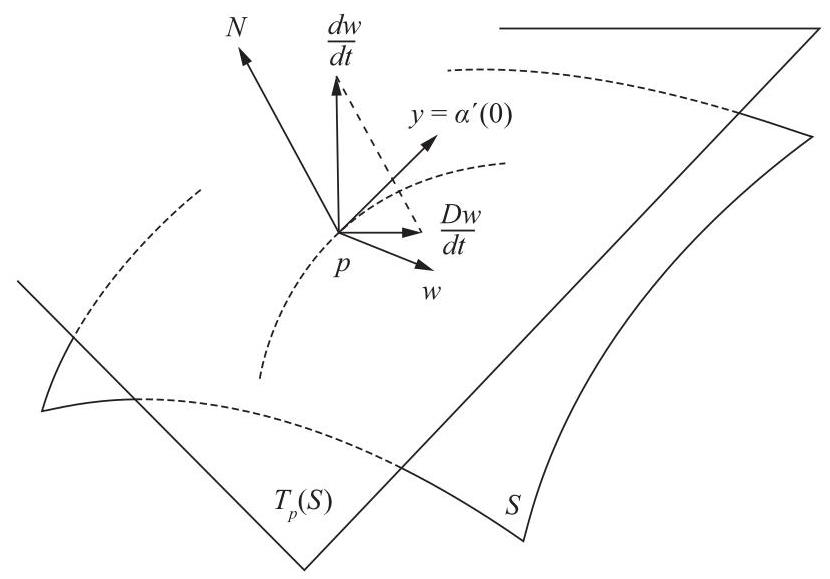
\includegraphics[max width=0.7\textwidth]{images/bo_d4b9jf3ef24c73e0334g_252_367_1462_830_579_0.jpg}
\end{center}
\hspace*{3em} 

图 4-8. 协变导数.

设 \(\mathbf{x}\left( {u\left( t\right) ,v\left( t\right) }\right)  = \alpha \left( t\right)\) 为曲线 \(\alpha\) 的表达式，且

\[
w\left( t\right)  = a\left( {u\left( t\right) ,v\left( t\right) }\right) {\mathbf{x}}_{u} + b\left( {u\left( t\right) ,v\left( t\right) }\right) {\mathbf{x}}_{v}
\]

\[
= a\left( t\right) {\mathbf{x}}_{u} + b\left( t\right) {\mathbf{x}}_{v},
\]

为 \(w\left( t\right)\) 在参数化 \(\mathbf{x}\left( {u,v}\right)\) 下的表达式.则

\[
\frac{dw}{dt} = a\left( {{\mathbf{x}}_{uu}{u}^{\prime } + {\mathbf{x}}_{uv}{v}^{\prime }}\right)  + b\left( {{\mathbf{x}}_{vu}{u}^{\prime } + {\mathbf{x}}_{vv}{v}^{\prime }}\right)  + {a}^{\prime }{\mathbf{x}}_{u} + {b}^{\prime }{\mathbf{x}}_{v},
\]

其中撇号表示关于 \(t\) 的导数.

由于 \({Dw}/{dt}\) 是 \({dw}/{dt}\) 在切平面上的分量，我们使用第 4-3 节式 (1) 中 \({\mathbf{x}}_{uu},{\mathbf{x}}_{uv}\) 和 \({\mathbf{x}}_{vv}\) 的表达式，并通过忽略法向分量，得到

\[
\frac{Dw}{dt} = \left( {{a}^{\prime } + {\Gamma }_{11}^{1}a{u}^{\prime } + {\Gamma }_{12}^{1}a{v}^{\prime } + {\Gamma }_{12}^{1}b{u}^{\prime } + {\Gamma }_{22}^{1}b{v}^{\prime }}\right) {\mathbf{x}}_{u} \tag{1}
\]

\[
+ \left( {{b}^{\prime } + {\mathbf{\Gamma }}_{11}^{2}a{u}^{\prime } + {\mathbf{\Gamma }}_{12}^{2}a{v}^{\prime } + {\mathbf{\Gamma }}_{12}^{2}b{u}^{\prime } + {\mathbf{\Gamma }}_{22}^{2}b{v}^{\prime }}\right) {\mathbf{x}}_{v}.
\]

式 (1) 表明 \({Dw}/{dt}\) 仅取决于向量 \(\left( {{u}^{\prime },{v}^{\prime }}\right)  = y\) 而不取决于曲线 \(\alpha\) .此外，曲面通过克里斯托费尔符号(即第一基本形式)出现在式 (1) 中.因此，我们的论断已得到证明.

特别地，如果 \(S\) 是一个平面，我们知道可以找到一个参数化，使得 \(E = G = 1\) 和 \(F = 0\) .快速检查给出克里斯托费尔符号的方程表明，在这种情况下， \({\mathbf{\Gamma }}_{ij}^{k}\) 变为零.在这种情况下，从式 (1) 可以得出，协变导数与平面中向量的通常导数一致(这也可以从定义 1 中几何上看出来).因此，协变导数是平面中向量通常导数的推广.

式 (1) 的另一个推论是，协变导数的定义可以扩展到仅在参数化曲线点上定义的向量场.为了弄清这一点，我们需要一些定义.

定义 2. 参数化曲线 \(\alpha  : \left\lbrack  {0,l}\right\rbrack   \rightarrow  S\) 是 \(\left( {0 - \epsilon ,l + \epsilon }\right) ,\epsilon  > 0\) 到 \(S\) 的可微映射在 \(\left\lbrack  {0,l}\right\rbrack\) 上的限制.如果 \(\alpha \left( 0\right)  = \mathrm{p}\) 和 \(\alpha \left( l\right)  = \mathrm{q}\) ，我们说 \(\alpha\) 连接 \(\mathrm{p}\) 到 \(\mathrm{q}.\alpha\) 是正则的，如果 \({\alpha }^{\prime }\left( t\right)  \neq  0\) 对于 \(\mathrm{t} \in  \left\lbrack  {0,l}\right\rbrack\) .

在接下来的讨论中，当终点 \(l\) 的指定不是必需的时，使用符号 \(\left\lbrack  {0,l}\right\rbrack   = I\) 会很方便.

定义 3. 设 \(\alpha  : \mathrm{I} \rightarrow  S\) 为 \(S\) 中的一条参数化曲线.沿着 \(\alpha\) 的 \(A\) 向量场 \(\mathrm{w}\) 是一个对应关系，它为每个 \(\mathrm{t} \in  \mathrm{I}\) 分配一个向量

\[
\mathrm{w}\left( \mathrm{t}\right)  \in  {\mathrm{T}}_{\alpha \left( \mathrm{t}\right) }\left( S\right) \text{ . }
\]

若在 \(\alpha \left( {\mathrm{t}}_{0}\right)\) 中存在某个参数化 \(\mathbf{x}\left( {\mathrm{u},\mathrm{v}}\right)\) ，使得 \(\mathrm{w}\left( \mathrm{t}\right)  = \mathrm{a}{\mathbf{x}}_{u} + \mathrm{b}{\mathbf{x}}_{v}\) 的分量 \(\mathrm{a}\left( \mathrm{t}\right) ,\mathrm{b}\left( \mathrm{t}\right)\) 在 \({\mathrm{t}}_{0}\) 处是 \(\mathrm{t}\) 的可微函数，则向量场 \(\mathrm{w}\) 在 \({\mathrm{t}}_{0} \in  \mathrm{I}\) 处可微.若 \(\mathrm{w}\) 对于每一个 \(\mathrm{t} \in  \mathrm{I}\) 都可微，则它在 \(\mathrm{I}\) 中可微.

沿 \(\alpha\) 的(可微)向量场的一个例子是 \(\alpha\) 的切向量场 \({\alpha }^{\prime }\left( t\right)\) (图 4-9).

\begin{center}
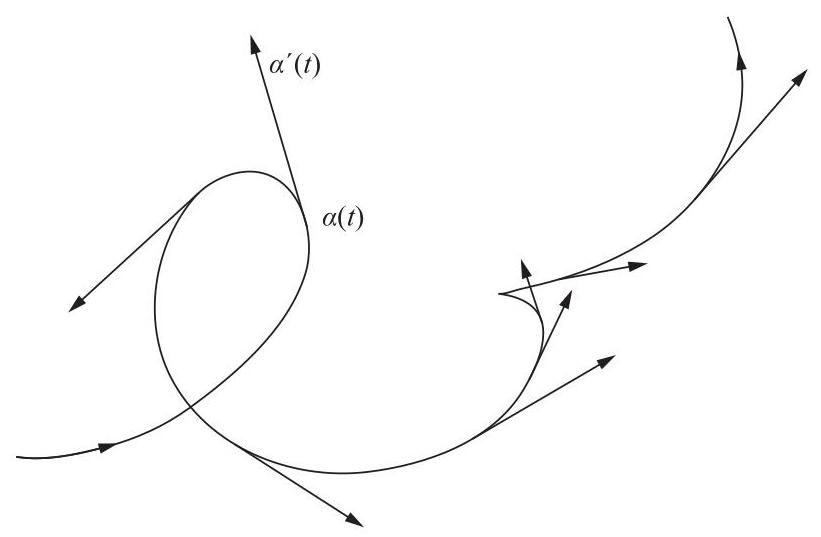
\includegraphics[max width=0.7\textwidth]{images/bo_d4b9jf3ef24c73e0334g_254_373_779_821_537_0.jpg}
\end{center}
\hspace*{3em} 

图 4-9. 沿曲线 \(\alpha\) 的切向量场.

定义 4. 设 \(\mathrm{w}\) 是沿 \(\alpha  : \mathrm{I} \rightarrow  S\) 的可微向量场.表达式 (1) 的 \(\left( {\mathrm{{Dw}}/\mathrm{{dt}}}\right) \left( \mathrm{t}\right) ,\mathrm{t} \in  \mathrm{I}\) 是良定义的，并称为 \(\mathrm{w}\) 在 \(\mathrm{t}\) 处的协变导数.

从曲面外部的视角来看，为了获得曲面 \(\alpha  : I \rightarrow  S\) 上向量场 \(w\) 在 \(t \in  I\) 处的协变导数，我们取 \(w\) 在 \(t\) 中的通常导数 \(\left( {{dw}/{dt}}\right) \left( t\right)\) ，并将该向量正交投影到切平面 \({T}_{\alpha \left( t\right) }\left( S\right)\) 上.由此可知，当两个曲面沿参数化曲线 \(\alpha\) 相切时，向量场 \(w\) 沿 \(\alpha\) 的协变导数对于两个曲面是相同的.

如果 \(\alpha \left( t\right)\) 是曲面 \(S\) 上的一条曲线，我们可以将其视为一个在曲面上运动的点的轨迹.此时 \({\alpha }^{\prime }\left( t\right)\) 是 \(\alpha\) 的速度， \({\alpha }^{\prime \prime }\left( t\right)\) 是其加速度.向量场 \({\alpha }^{\prime }\left( t\right)\) 的协变导数 \(D{\alpha }^{\prime }/{dt}\) 是加速度 \({\alpha }^{\prime \prime }\left( t\right)\) 的切向分量.直观地说， \(D{\alpha }^{\prime }/{dt}\) 是点 \(\alpha \left( t\right)\) “从曲面 \(S\) 看到的”加速度.

定义 5. 沿参数化曲线 \(\alpha  : \mathrm{I} \rightarrow  S\) 的向量场 \(\mathrm{w}\) 被称为平行，如果对于每一点 \(\mathrm{t} \in  \mathrm{I}\) ， \(\mathrm{{Dw}}/\mathrm{{dt}} = 0\) 都成立.

在平面这个特例中，沿参数化曲线的平行场概念简化为沿曲线的常数场；也就是说，向量的长度及其与固定方向的夹角是恒定的(图 4-10).以下命题表明，这些性质在任何曲面上都部分地得以保留.

\begin{center}
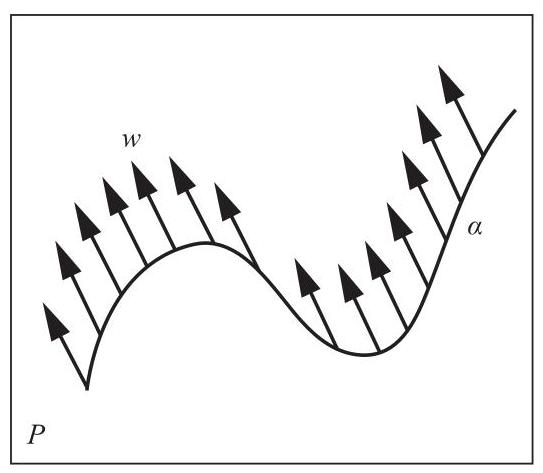
\includegraphics[max width=0.4\textwidth]{images/bo_d4b9jf3ef24c73e0334g_255_182_588_543_473_0.jpg}
\end{center}
\hspace*{3em} 

图 4-10

命题 1. 设 \(\mathrm{w}\) 和 \(\mathrm{v}\) 是 \(\alpha  : \mathrm{I} \rightarrow  S\) 上的平行向量场.则 \(\langle \mathrm{w}\left( \mathrm{t}\right) ,\mathrm{v}\left( \mathrm{t}\right) \rangle\) 是常数.特别地， \(\left| {\mathrm{w}\left( \mathrm{t}\right) }\right|\) 和 \(\left| {\mathrm{v}\left( \mathrm{t}\right) }\right|\) 是常数， \(\mathrm{v}\left( \mathrm{t}\right)\) 和 \(\mathrm{w}\left( \mathrm{t}\right)\) 之间的夹角是常数.

证明.说向量场 \(w\) 沿 \(\alpha\) 是平行的，意味着 \({dw}/{dt}\) 垂直于在 \(\alpha \left( t\right)\) 处与曲面相切的平面；也就是说，

\[
\left\langle  {v\left( t\right) ,{w}^{\prime }\left( t\right) }\right\rangle   = 0,\;t \in  I.
\]

另一方面， \({v}^{\prime }\left( t\right)\) 也垂直于 \(\alpha \left( t\right)\) 处的切平面.因此，

\[
\langle v\left( t\right) ,w\left( t\right) {\rangle }^{\prime } = \left\langle  {{v}^{\prime }\left( t\right) ,w\left( t\right) }\right\rangle   + \left\langle  {v\left( t\right) ,{w}^{\prime }\left( t\right) }\right\rangle   = 0;
\]

也就是说， \(\langle v\left( t\right) ,w\left( t\right) \rangle  =\) 是常数.Q.E.D.

当然，在任意曲面上，平行场可能看起来与我们的 \({R}^{3}\) 直觉不符.例如，单位球 \({S}^{2}\) 的一条经线(由弧长参数化)的切向量场是 \({S}^{2}\) 上的一个平行场(图 4-11).事实上，由于经线是 \({S}^{2}\) 上的一个大圆，该场通常的导数垂直于 \({S}^{2}\) .因此，其协变导数为零.

以下命题表明，存在参数化曲线 \(\alpha \left( t\right)\) 上的平行向量场，并且它们由它们在某点 \({t}_{0}\) 的值完全确定.

\begin{center}
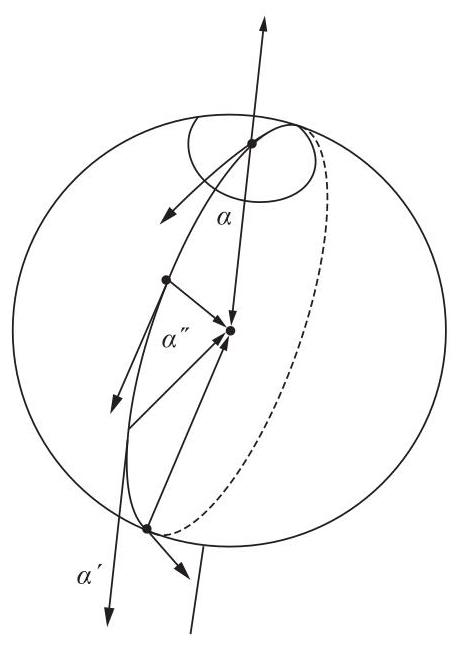
\includegraphics[max width=0.4\textwidth]{images/bo_d4b9jf3ef24c73e0334g_256_197_190_459_648_0.jpg}
\end{center}
\hspace*{3em} 

图 4-11. 球面上的平行场.

命题 2. 设 \(\alpha  : \mathrm{I} \rightarrow  S\) 是 \(S\) 中的一个参数化曲线，设 \({\mathrm{w}}_{0} \in  {\mathrm{T}}_{\alpha \left( {\mathrm{t}}_{0}\right) }\left( S\right) ,{\mathrm{t}}_{0} \in  \mathrm{I}\) .则存在一个唯一的平行向量场 \(\mathrm{w}\left( \mathrm{t}\right)\) 沿 \(\alpha \left( \mathrm{t}\right)\) ，使得 \(\mathrm{w}\left( {\mathrm{t}}_{0}\right)  = {\mathrm{w}}_{0}\) .

命题 2 的一个初等证明将在本节稍后给出.然而，熟悉 3-4 节内容的读者会注意到，该证明是微分方程存在唯一性定理的直接推论.

命题 2 允许我们讨论向量沿参数化曲线的平行移动.

定义 6. 设 \(\alpha  : \mathrm{I} \rightarrow  S\) 是一个参数化曲线， \({\mathrm{w}}_{0} \in \; {\mathrm{T}}_{\alpha \left( {\mathrm{t}}_{0}\right) }\left( S\right) ,{\mathrm{t}}_{0} \in  \mathrm{I}\) .设 \(\mathrm{w}\) 是沿 \(\alpha\) 的平行向量场，使得 \(\mathrm{w}\left( {\mathrm{t}}_{0}\right)  = {\mathrm{w}}_{0}\) .向量 \(\mathrm{w}\left( {\mathrm{t}}_{1}\right) ,{\mathrm{t}}_{1} \in  \mathrm{I}\) 被称为向量 \({\mathrm{w}}_{0}\) 沿 \(\alpha\) 在点 \({\mathrm{t}}_{1}\) 的平行移动.

应该指出，如果 \(\alpha  : I \rightarrow  S,t \in  I\) 是正则的，那么平行移动不依赖于 \(\alpha \left( I\right)\) 的参数化.事实上，如果 \(\beta  : J \rightarrow  S,\sigma  \in  J\) 是 \(\alpha \left( I\right)\) 的另一个正则参数化，则由式 (1) 可知

\[
\frac{Dw}{d\sigma } = \frac{Dw}{dt}\frac{dt}{d\sigma },\;t \in  I,\sigma  \in  J.
\]

当且仅当 \(w\left( \sigma \right)\) 是平行的， \({dt}/{d\sigma } \neq  0,w\left( t\right)\) 才是平行的.

命题 1 包含平行移动的一个有趣性质.固定两个点 \(p,q \in  S\) 和一个参数化曲线 \(\alpha  : I \rightarrow  S\) ，其中 \(\alpha \left( 0\right)  = p\) ， \(\alpha \left( 1\right)  = q\) .令 \({P}_{\alpha } : {T}_{p}\left( S\right)  \rightarrow  {T}_{q}\left( S\right)\) 为将每个 \(v \in \; {T}_{p}\left( S\right)\) 沿 \(\alpha\) 在 \(q\) 处映射到其平行移动的映射.命题 1 表明该映射是一个线性等距变换.

平行移动的另一个有趣性质是，如果两个曲面 \(S\) 和 \(\bar{S}\) 沿参数化曲线 \(\alpha\) 和 \({w}_{0}\) 相切，并且 \({T}_{\alpha \left( {t}_{0}\right) }\left( S\right)  = \; {T}_{\alpha \left( {t}_{0}\right) }\left( \bar{S}\right)\) 是 \(S\) 的一个向量，那么当且仅当 \(w\left( t\right)\) 是 \({w}_{0}\) 相对于曲面 \(\bar{S}\) 的平行移动时， \(w\left( t\right)\) 才是 \({w}_{0}\) 相对于曲面 \(S\) 的平行移动.事实上， \(w\) 的协变导数 \({Dw}/{dt}\) 对于两个曲面是相同的.由于平行移动是唯一的，因此该断言成立.

上述性质将使我们能够给出一个简单且有启发性的平行移动的例子.

示例 1. 设 \(C\) 为一个定向单位球的余纬度 \(\varphi\) 的平行圈(见图 4-12)，设 \({w}_{0}\) 为一个单位向量，在 \(C\) 的某点 \(p\) 处切于 \(C\) .我们沿 \(C\) 来确定 \({w}_{0}\) 的平行移动，其中 \(C\) 由弧长 \(s\) 参数化，且在 \(p\) 处有 \(s = 0\) .

\begin{center}
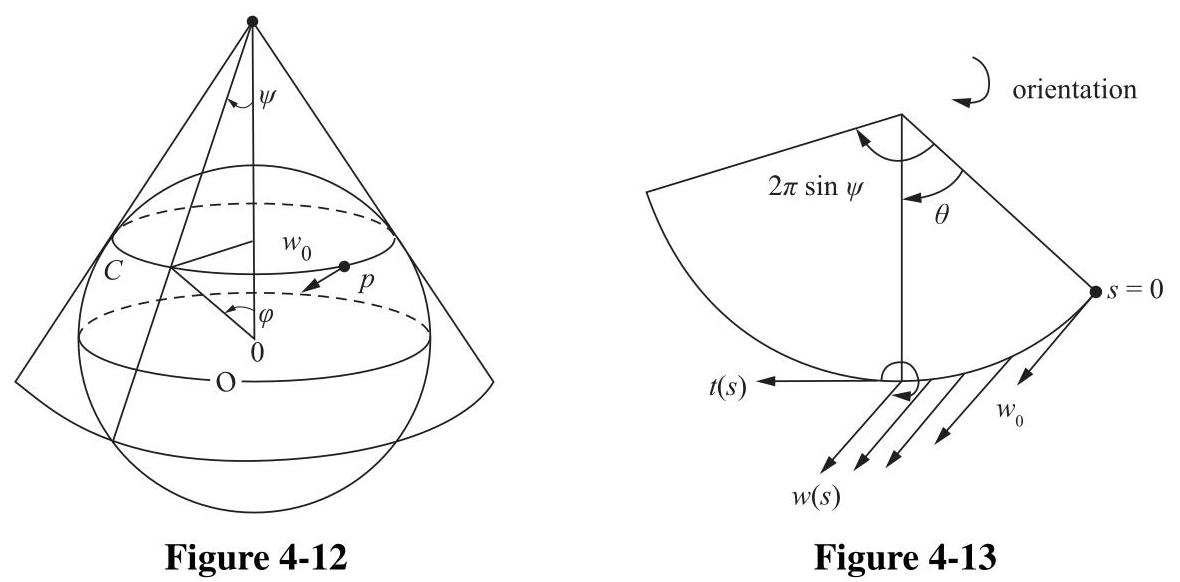
\includegraphics[max width=1.0\textwidth]{images/bo_d4b9jf3ef24c73e0334g_257_178_805_1180_582_0.jpg}
\end{center}
\hspace*{3em} 

考虑沿 \(C\) 切于球面的圆锥.该圆锥顶点处的角度 \(\psi\) 由 \(\psi  = \left( {\pi /2}\right)  - \varphi\) 给出.根据上述性质，问题简化为确定 \({w}_{0}\) 沿 \(C\) 相对于切面圆锥的平行移动.

然而，除去一条母线的圆锥与一个开集 \(U \subset  {R}^{2}\) 等距(参见第 4-2 节例 3)，该开集用极坐标表示为

\[
0 < p <  + \infty ,\;0 < \theta  < {2\pi }\sin \psi .
\]

由于在平面上，平行移动与通常的概念一致，对于 \(p\) 的一个位移 \(s\) ，对应于中心角 \(\theta\) (参见图 4-13)，我们得到切向量 \(t\left( s\right)\) 与平行移动 \(w\left( s\right)\) 形成的定向角由 \({2\pi } - \theta\) 给出.

有时引入“折线”的概念会更方便，这可以表述如下.

定义 7. 一个映射 \(\alpha  : \left\lbrack  {0,l}\right\rbrack   \rightarrow  S\) 是一个分段正则参数化曲线，如果 \(\alpha\) 是连续的，并且存在一个细分

\[
0 = {\mathrm{t}}_{0} < {\mathrm{t}}_{1} < \cdots  < {\mathrm{t}}_{\mathrm{k}} < {\mathrm{t}}_{\mathrm{k} + 1} = l
\]

以这样的方式对区间 \(\left\lbrack  {0,l}\right\rbrack\) 进行参数化，使得其限制 \(\alpha  \mid  \left\lbrack  {{\mathrm{t}}_{\mathrm{i}},{\mathrm{t}}_{\mathrm{i} + 1}}\right\rbrack  ,\mathrm{i} = 0,\ldots ,\mathrm{k}\) 是一条正则曲线.每一条 \(\alpha  \mid  \left\lbrack  {{\mathrm{t}}_{\mathrm{i}},{\mathrm{t}}_{\mathrm{i} + 1}}\right\rbrack\) 都称为 \(\alpha\) 的正则弧.

平行移动的概念可以很容易地推广到参数化的分段正则曲线.例如，如果初始值 \({w}_{0}\) 位于区间 \(\left\lbrack  {{t}_{i},{t}_{i + 1}}\right\rbrack\) 中，我们在正则弧 \(\alpha  \mid  \left\lbrack  {{t}_{i},{t}_{i + 1}}\right\rbrack\) 上进行通常的平行移动；如果 \({t}_{i + 1} \neq  l\) ，我们将 \(w\left( {t}_{i + 1}\right)\) 作为下一个弧 \(\alpha  \mid  \left\lbrack  {{t}_{i + 1},{t}_{i + 2}}\right\rbrack\) 上平行移动的初始值，依此类推.

例 2. \({}^{ \dagger  }\) 前面的例子是平行移动的一个有趣几何构造的特例.设 \(C\) 是曲面 \(S\) 上的一条正则曲线，并假设 \(C\) 在任何地方都不与渐近方向相切.考虑 \(S\) 沿 \(C\) 的切平面族的外包线(参见第 3-5 节例 4).在 \(C\) 的邻域中，这个外包线是一个正则曲面 \(\sum\) ，它沿 \(C\) 与 \(S\) 相切.(在例 1 中， \(\sum\) 可以取为圆锥上围绕 \(C\) 的一个带，该圆锥沿 \(C\) 与球面相切.)因此，无论我们是相对于 \(S\) 还是 \(\sum\) 来考虑，沿 \(C\) 的任何向量 \(w \in  {T}_{p}\left( S\right) ,p \in  S\) 的平行移动都是相同的.此外， \(\sum\) 是一个可展曲面；因此，其高斯曲率为零.

现在，我们将在本书后面(第 4-6 节，Minding 定理)证明，高斯曲率为零的曲面在局部上与平面等距.因此，我们可以通过一个等距变换 \(\varphi  : V \rightarrow  P\) 将 \(p\) 的一个邻域 \(V \subset  \sum\) 映射到一个平面 \(P\) .为了得到 \(V \cap  C\) 上的 \(w\) 的平行移动，我们在 \(d{\varphi }_{p}\left( w\right)\) 的平面上进行通常的平行移动，沿 \(\varphi \left( C\right)\) ，然后通过 \({d\varphi }\) 将其拉回到 \(\sum\) (图 4-14).

这为沿 \(C\) 的小弧的平行移动提供了一个几何构造.我们将其留作练习，以证明此构造可以逐步扩展到给定的 \(C\) 弧.(使用 Heine-Borel 定理，并按照折线的情况进行.)

平面上参数化曲线 \(\gamma  : I \rightarrow  {R}^{2}\) ，其切向量场 \({\gamma }^{\prime }\left( t\right)\) 平行，正是该平面的直线.满足曲面上类似条件的参数化曲线称为测地线.

定义 8. 一个非常值、参数化的曲线 \(\gamma  : \mathrm{I} \rightarrow  S\) 在 \(\mathrm{t} \in  \mathrm{I}\) 处被称为测地线，如果其切向量场 \({\gamma }^{\prime }\left( \mathrm{t}\right)\) 沿 \(\gamma\) 在 \(\mathrm{t}\) 处是平行的话；也就是说，

\[
\frac{\mathrm{D}{\gamma }^{\prime }\left( \mathrm{t}\right) }{\mathrm{{dt}}} = 0;
\]



†本例使用了第 3-5 节关于直纹曲面的材料.



\begin{center}
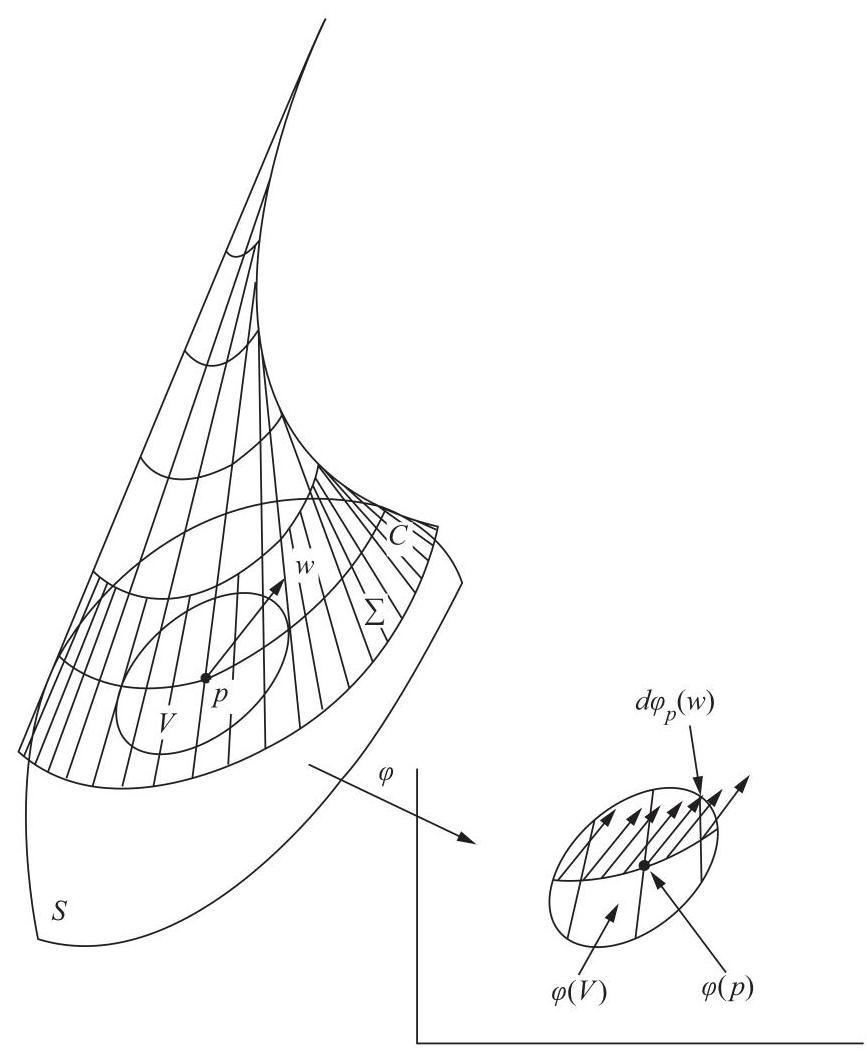
\includegraphics[max width=0.7\textwidth]{images/bo_d4b9jf3ef24c73e0334g_259_326_188_867_1055_0.jpg}
\end{center}
\hspace*{3em} 

图 4-14. 沿 \(C\) 的平行移动.

如果 \(\gamma\) 对于所有 \(\mathrm{t} \in  \mathrm{I}\) 都是测地线，则称 \(\gamma\) 是参数化测地线.

根据命题 1，我们立即得到 \(\left| {{\gamma }^{\prime }\left( t\right) }\right|  =\) 是常数 \(= c \neq  0\) .因此，我们可以引入弧长 \(s = {ct}\) 作为参数，并得出参数化测地线 \(\gamma\) 的参数 \(t\) 与 \(\gamma\) 的弧长成正比.

请注意，参数化测地线可能存在自交点.(例 6 将说明这一点；参见图 4-20.)然而，其切向量永远不为零，因此参数化是正则的.

测地线的概念显然是局部的.先前的讨论允许我们将测地线的定义扩展到 \(S\) 的正则曲线子集.

定义 8a. \(S\) 中的一个正则连通曲线 \(\mathrm{C}\) 被称为 \(a\) 测地线，如果对于每一个 \(\mathrm{p} \in  \mathrm{C}\) ，通过弧长 \(S\) 的坐标邻域 \(\mathrm{p}\) 的参数化 \(\alpha \left( S\right)\) 是一个参数化测地线；也就是说， \({\alpha }^{\prime }\left( S\right)\) 是沿 \(\alpha \left( S\right)\) 的平行向量场.

请注意，包含在曲面上的每条直线都满足定义 8a.

从曲面 \(S\) 的外部来看，定义 8a 等价于说 \({\alpha }^{\prime \prime }\left( s\right)  = {kn}\) 垂直于切平面，也就是说，平行于曲面的法线.换句话说，一条正则曲线 \(C \subset  S\left( {k \neq  0}\right)\) 是测地线当且仅当其在每一点 \(p \in  C\) 的主法线平行于 \(S\) 在 \(p\) 处的法线.

上述性质可用于通过几何方式识别某些测地线，如下例所示.

例 3. 球体 \({S}^{2}\) 的大圆是测地线.事实上，大圆 \(C\) 是通过与通过球心 \(O\) 的平面相交得到的.在某点 \(p \in  C\) 的主法线位于连接 \(p\) 和 \(O\) 的直线的方向上，因为 \(C\) 是以 \(O\) 为中心的圆.由于 \({S}^{2}\) 是一个球体，法线位于同一方向，这验证了我们的说法.

在本节后面，我们将证明一个普遍事实:对于每一点 \(p \in  S\) 和 \({T}_{p}\left( S\right)\) 中的每个方向，都存在唯一一条通过 \(p\) 且切线方向为此方向的测地线 \(C \subset  S\) .对于球体的情况，通过每一点和切线方向的每条方向都恰好有一条大圆，正如我们之前证明的，它是一条测地线.因此，根据唯一性，大圆是球体的唯一测地线.

例 4. 对于圆 \({x}^{2} + {y}^{2} = 1\) 上的正圆柱体，很明显，通过圆柱体与垂直于圆柱体轴线的平面相交得到的圆是测地线.这是因为其任意点的法线平行于该点处曲面的法线.

另一方面，根据定义 8a 后的观察，圆柱体的直线(母线)也是测地线.

为了验证圆柱体上是否存在其他测地线 \(C\) ，我们将考虑一个参数化(参见示例 2，第 2-5 节)

\[
\mathbf{x}\left( {u,v}\right)  = \left( {\cos u,\sin u,v}\right)
\]

在圆柱体上的一个点 \(p \in  C\) ，具有 \(\mathbf{x}\left( {0,0}\right)  = p\) .在此参数化中，曲线 \(\mathbf{\Gamma }\) 上的一个邻域 \(p\) 由 \(\mathbf{x}\left( {u\left( s\right) ,v\left( s\right) }\right)\) 表示，其中 \(s\) 是 \(\mathbf{\Gamma }\) 的弧长.正如我们之前所见(参见示例 1，第 4-2 节)， \(\mathbf{x}\) 是一个局部等距变换，将 \({uv}\) 平面上的 \(\left( {0,0}\right)\) 的邻域 \(U\) 映射到圆柱体上.由于测地线的条件是局部的且等距变换不变，因此曲线 \(\left( {u\left( s\right) ,v\left( s\right) }\right)\) 必须是 \(U\) 中通过 \(\left( {0,0}\right)\) 的测地线.但平面上的测地线是直线.因此，排除已获得的情况，

\[
u\left( s\right)  = {as},\;v\left( s\right)  = {bs},\;{a}^{2} + {b}^{2} = 1.
\]

由此可知，当一条正则曲线 \(\mathbf{\Gamma }\) (既不是圆也不是直线)是圆柱体的测地线时，它在局部上具有(图 4-15)的形式

\[
\text{ (cos }{as}\text{ , }\sin {as},{bs}\text{ ), }
\]

因此它是一条螺旋线.这样，就确定了所有直圆柱体的测地线.

\begin{center}
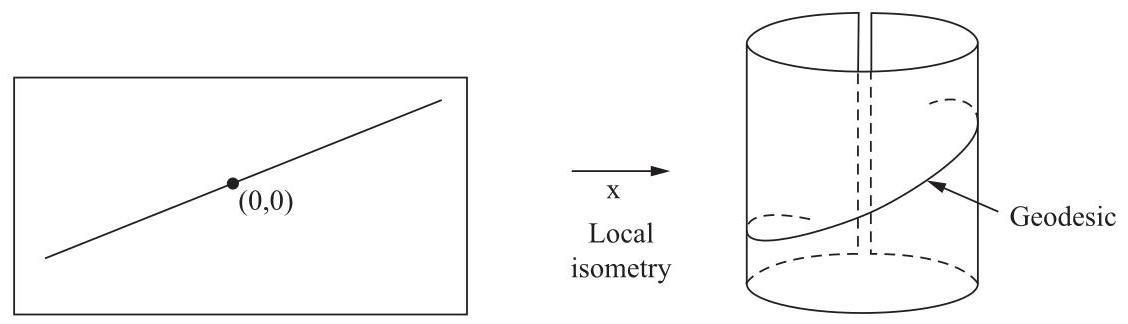
\includegraphics[max width=1.0\textwidth]{images/bo_d4b9jf3ef24c73e0334g_261_202_616_1128_324_0.jpg}
\end{center}
\hspace*{3em} 

图 4-15. 圆柱体上的测地线.

观察到，给定圆柱体上不位于平行于 \({xy}\) 平面的圆上的两点，可以通过无限多条螺旋线连接它们.这一事实意味着，与平面上的情况不同，圆柱体上的两点通常可以通过无限多条测地线连接.观察到这种情况只可能发生在那些“完整转一圈”的测地线上，因为圆柱体减去一条母线与平面(图 4-16)是等距的.

\begin{center}
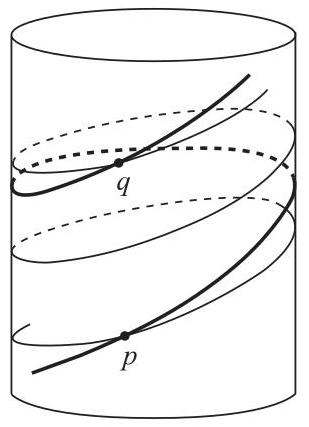
\includegraphics[max width=0.2\textwidth]{images/bo_d4b9jf3ef24c73e0334g_261_182_1479_309_427_0.jpg}
\end{center}
\hspace*{3em} 

图 4-16. 连接 \(p\) 和 \(q\) 的圆柱体上的两条测地线.

继续类比平面，我们观察到直线，即平面的测地线，也具有曲率为零的正则曲线的特征.现在，定向平面曲线的曲率由切向于该曲线的单位向量场的导数的绝对值给出，并带有一个符号，该符号表示曲线相对于平面方向的凹度(参见第 1-5 节，备注 1).为了考虑符号，引入以下定义是方便的.

定义 9. 令 \(\mathrm{W}\) 为定向曲面 \(S\) 上参数化曲线 \(\alpha  : \mathrm{I} \rightarrow  S\) 上的单位向量的可微场.由于 \(\mathrm{w}\left( \mathrm{t}\right) ,\mathrm{t} \in  \mathrm{I}\) 是单位向量场， \(\left( {\mathrm{{dw}}/\mathrm{{dt}}}\right) \left( \mathrm{t}\right)\) 垂直于 \(\mathrm{w}\left( \mathrm{t}\right)\) ，因此

\[
\frac{\mathrm{D}\mathrm{w}}{\mathrm{{dt}}} = \lambda \left( {N \land  \mathrm{w}\left( \mathrm{t}\right) }\right) .
\]

实数 \(\lambda  = \lambda \left( \mathrm{t}\right)\) ，记作 [Dw/dt]，称为 \(\mathrm{w}\) 在 \(\mathrm{t}\) 处的协变导数的代数值.

观察到 \(\left\lbrack  {{Dw}/{dt}}\right\rbrack\) 的符号取决于 \(S\) 的方向以及 \(\left\lbrack  {{Dw}/{dt}}\right\rbrack   = \langle {dw}/{dt},N \land  w\rangle .\)

我们还应作一般性说明，从现在起， \(S\) 的定向将在要介绍的概念中起至关重要的作用.细心的读者会注意到，平行移动和测地的定义不依赖于 \(S\) 的定向.相比之下，下面将定义的测地曲率，在 \(S\) 的定向改变时会改变符号.

现在，我们将为曲面上的曲线定义一个概念，它是平面曲线曲率的类似物.

定义 10. 设 \(\mathrm{C}\) 是包含在定向曲面 \(S\) 中的定向正则曲线，设 \(\alpha \left( S\right)\) 是 \(\mathrm{C}\) 在 \(\mathrm{p} \in  S\) 邻域内的参数化，参数为弧长 \(S\) . \({\alpha }^{\prime }\left( S\right)\) 在 \(\mathrm{p}\) 处的协变导数 \(\left\lbrack  {\mathrm{D}{\alpha }^{\prime }\left( S\right) /\mathrm{{ds}}}\right\rbrack   = {\mathrm{k}}_{\mathrm{g}}\) 的代数值称为 \(\mathrm{C}\) 在 \(\mathrm{p}\) 处的测地曲率.

因此，正则曲线的测地线被表征为测地曲率为零的曲线.

从曲面外部的观点来看， \(C\) 在 \(p\) 处的 \({k}_{g}\) 的测地曲率的绝对值是向量 \({\alpha }^{\prime \prime }\left( s\right)  = {kn}\) 的切向分量的绝对值，其中 \(k\) 是 \(C\) 在 \(p\) 处的曲率， \(n\) 是 \(C\) 在 \(p\) 处的法向量.回想一下，向量 \({kn}\) 的法向分量的绝对值是 \(C \subset  S\) 在 \(p\) 中的 \({k}_{n}\) 的法曲率的绝对值，我们立即得到(图 4-17)

\[
{k}^{2} = {k}_{g}^{2} + {k}_{n}^{2}.
\]

例如，单位球 \({S}^{2}\) 中，余纬 \(\varphi\) 的平行线 \(C\) 的 \({k}_{g}\) 的测地曲率的绝对值可以从关系式(见图 4-18)计算得出

\[
\frac{1}{{\sin }^{2}\varphi } = {k}_{n}^{2} + {k}_{g}^{2} = 1 + {k}_{g}^{2}
\]

\begin{center}
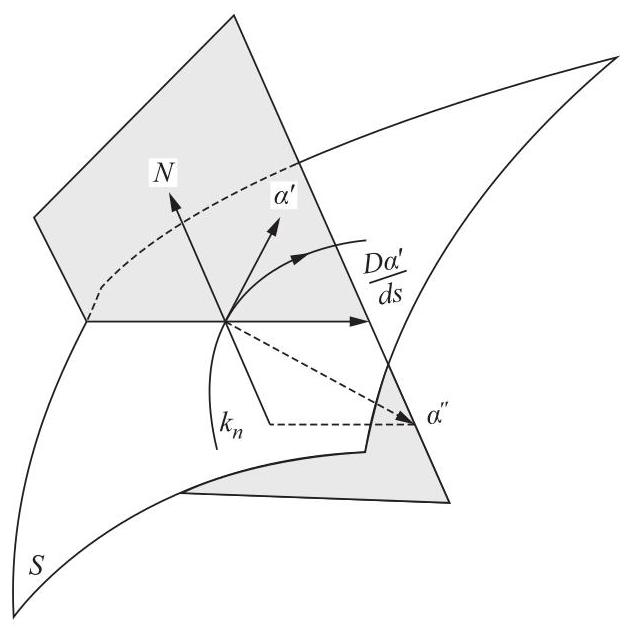
\includegraphics[max width=0.5\textwidth]{images/bo_d4b9jf3ef24c73e0334g_263_180_190_626_630_0.jpg}
\end{center}
\hspace*{3em} 

图 4-17

\(\left| {k}_{\mathrm{g}}\right|  = \left| {\operatorname{cotan}\varphi }\right|\)

\(C \; \sin \varphi\)

\(\pi /2 - \varphi\)

1

图 4-18. 单位球上平行线的测地曲率.

即，

\[
{k}_{g}^{2} = {\operatorname{cotan}}^{2}\varphi
\]

\({k}_{g}\) 的符号取决于 \({S}^{2}\) 和 \(C\) 的定向.

从外部解释得出的另一个结论是，当两个曲面沿着一条正则曲线 \(C\) 相切时， \(C\) 的测地曲率的绝对值相对于这两个曲面中的任何一个都是相同的.

注. 当我们改变 \(C\) 或 \(S\) 的定向时， \(C \subset  S\) 的测地曲率会改变符号.

现在我们将得到协变导数代数值的表达式(命题 3 如下).为此，我们需要一些准备工作.

设 \(v\) 和 \(w\) 是参数化曲线 \(\alpha  : I \rightarrow  S\) 沿下的两个可微向量场，其中 \(\left| {v\left( t\right) }\right|  = \left| {w\left( t\right) }\right|  = 1,t \in  I\) .我们想定义一个可微函数 \(\varphi  : I \rightarrow  R\) ，使得 \(\varphi \left( t\right) ,t \in  I\) 是 \(S\) 的定向下从 \(v\left( t\right)\) 到 \(w\left( t\right)\) 的角度的确定值.为此，我们考虑沿 \(\alpha\) 的可微向量场 \(\bar{v}\) ，它由条件定义，即 \(\{ v\left( t\right) ,\bar{v}\left( t\right) \}\) 对于每个 \(t \in  I\) 都是一个标准正交正基.因此， \(w\left( t\right)\) 可以表示为

\[
w\left( t\right)  = a\left( t\right) v\left( t\right)  + b\left( t\right) \bar{v}\left( t\right) ,
\]

其中 \(a\) 和 \(b\) 是 \(I\) 和 \({a}^{2} + {b}^{2} = 1\) 中的可微函数.

下面的引理 1 表明，通过固定从 \(v\left( {t}_{0}\right)\) 到 \(w\left( {t}_{0}\right)\) 的角度的确定性 \({\varphi }_{0}\) ，可以将其在 \(I\) 中可微地“扩展”，从而得到所需的函数.

引理 1. 令 a 和 \(\mathrm{b}\) 为 I 中的可微函数，且 \({\mathrm{a}}^{2} + {\mathrm{b}}^{2} = 1\) 和 \({\varphi }_{0}\) 满足 \(\mathrm{a}\left( {\mathrm{t}}_{0}\right)  = \cos {\varphi }_{0},\mathrm{\;b}\left( {\mathrm{t}}_{0}\right)  = \sin {\varphi }_{0}\) .则可微函数

\[
\varphi  = {\varphi }_{0} + {\int }_{{\mathrm{t}}_{0}}^{\mathrm{t}}\left( {{\mathrm{{ab}}}^{\prime } - {\mathrm{{ba}}}^{\prime }}\right) \mathrm{{dt}}
\]

满足 \(\cos \varphi \left( \mathrm{t}\right)  = \mathrm{a}\left( \mathrm{t}\right) ,\sin \varphi \left( \mathrm{t}\right)  = \mathrm{b}\left( \mathrm{t}\right) ,\mathrm{t} \in  \mathrm{I}\) ，且 \(\varphi \left( {\mathrm{t}}_{0}\right)  = {\varphi }_{0}\) .

证明. 只需证明函数

\[
{\left( a - \cos \varphi \right) }^{2} + {\left( b - \sin \varphi \right) }^{2} = 2 - 2\left( {a\cos \varphi  + b\sin \varphi }\right)
\]

恒等于零，或者

\[
A = a\cos \varphi  + b\sin \varphi  = 1.
\]

利用 \(a{a}^{\prime } =  - b{b}^{\prime }\) 的事实以及 \(\varphi\) 的定义，我们很容易得到

\[
{A}^{\prime } =  - a\left( {\sin \varphi }\right) {\varphi }^{\prime } + b\left( {\cos \varphi }\right) {\varphi }^{\prime } + {a}^{\prime }\cos \varphi  + {b}^{\prime }\sin \varphi
\]

\[
=  - {b}^{\prime }\left( {\sin \varphi }\right) \left( {{a}^{2} + {b}^{2}}\right)  - {a}^{\prime }\left( {\cos \varphi }\right) \left( {{a}^{2} + {b}^{2}}\right)
\]

\[
+ {a}^{\prime }\cos \varphi  + {b}^{\prime }\sin \varphi  = 0.
\]

因此， \(A\left( t\right)  =\) 为常数，且由于 \(A\left( {t}_{0}\right)  = 1\) ，引理得证.证毕.

现在我们可以将两条单位向量场沿曲线的协变导数与它们形成的夹角的变化联系起来.

引理 2. 令 \(\mathrm{v}\) 和 \(\mathrm{w}\) 为沿曲线 \(\alpha  : \mathrm{I} \rightarrow  S\) 的两个可微向量场，且 \(\left| {\mathrm{w}\left( \mathrm{t}\right) }\right|  = \left| {\mathrm{v}\left( \mathrm{t}\right) }\right|  = 1,\mathrm{t} \in  \mathrm{I}\) .则

\[
\left\lbrack  \frac{\mathrm{{Dw}}}{\mathrm{{dt}}}\right\rbrack   - \left\lbrack  \frac{\mathrm{{Dv}}}{\mathrm{{dt}}}\right\rbrack   = \frac{\mathrm{d}\varphi }{\mathrm{{dt}}},
\]

其中 \(\varphi\) 是从 \(\mathrm{v}\) 到 \(\mathrm{w}\) 的角度的一个可微确定性，如引理 1 所给出.

证明. 我们首先证明引理对于 \(\varphi  \neq  0\) .由于 \(\langle v,w\rangle  = \cos \varphi\) ，我们得到

\[
\left\langle  {{v}^{\prime },w}\right\rangle   + \left\langle  {v,{w}^{\prime }}\right\rangle   =  - \sin \varphi {\varphi }^{\prime }, \tag{2}
\]

因此

\[
\langle {Dv}/{dt},w\rangle  + \langle v,{Dw}/{dt}\rangle  = \sin \varphi {\varphi }^{\prime }.
\]

但是

\[
\langle {Dv}/{dt},w\rangle  + \langle {\lambda N} \land  v,w\rangle  = \left\lbrack  {{Dv}/{dt}}\right\rbrack   < N \land  v,w\rangle .
\]

因此，我们可以将 (2) 的左侧写成

\[
\langle {Dv}/{dt},w\rangle  + \langle v,{Dw}/{dt}\rangle  = \left\lbrack  {{Dv}/{dt}}\right\rbrack   < N \land  v,w\rangle  + \left\lbrack  {{Dw},{dt}}\right\rbrack  \langle v,N \land  w\rangle
\]

\[
= \left( {\left\lbrack  {{Dv}/{dt}}\right\rbrack   - \left\lbrack  {{Dw},{dt}}\right\rbrack  }\right)  < N \land  v,w\rangle .
\]

由此可知

\[
\left( {\left\lbrack  {{Dv}/{dt}}\right\rbrack   - \left\lbrack  {{Dw}/{dt}}\right\rbrack  }\right) \sin \varphi  = \sin \varphi {\varphi }^{\prime }
\]

这证明了引理对 \(\varphi  \neq  0\) 成立.

如果 \(\varphi  = 0\) 在 \(p\) 处，那么在 \(p\) 的某个邻域 \(U\) 中存在 \(\varphi  \equiv  0\) ，或者存在一个序列 \(\left( {p}_{n}\right)  \rightarrow  p\) 满足 \(\varphi \left( {p}_{n}\right)  \neq  0\) .在第一种情况下， \({\varphi }^{\prime } \equiv  0\) 在 \(U,v = w\) 中，引理显然成立.在第二种情况下，引理通过连续性成立.

Q.E.D.

上述引理的一个直接推论是以下观察.设 \(C\) 是 \(S,\alpha \left( s\right)\) 上的一个正则定向曲线，其参数化由弧长 \(s\) 在 \(p \in  C\) 处给出，并且 \(v\left( s\right)\) 是 \(\alpha \left( s\right)\) 上的一个平行场.那么，通过取 \(w\left( s\right)  = {\alpha }^{\prime }\left( s\right)\) ，我们得到

\[
{k}_{g}\left( s\right)  = \left\lbrack  \frac{D{\alpha }^{\prime }\left( s\right) }{ds}\right\rbrack   = \frac{d\varphi }{ds}.
\]

换句话说，测地曲率是曲线切线与曲线上的平行方向所成角度的变化率.在平面情况下，平行方向是固定的，测地曲率简化为通常的曲率.

现在我们可以得到协变导数的代数值的预期表达式.每当我们谈论定向曲面的参数化时，都假定该参数化与给定的方向兼容.

命题 3. 设 \(x\left( {\mathrm{u},\mathrm{v}}\right)\) 是定向曲面 \(S\) 的邻域的正交参数化(即 \(\mathrm{F} = 0\) )，并且 \(\mathrm{w}\left( \mathrm{t}\right)\) 是沿曲线 \(\mathbf{x}\left( {\mathrm{u}\left( \mathrm{t}\right) ,\mathrm{v}\left( \mathrm{t}\right) }\right)\) 的单位向量的可微场.那么

\[
\left\lbrack  \frac{\mathrm{{Dw}}}{\mathrm{{dt}}}\right\rbrack   = \frac{1}{2\sqrt{\mathrm{{EG}}}}\left\{  {{\mathrm{G}}_{\mathrm{u}}\frac{\mathrm{{dv}}}{\mathrm{{dt}}} - {\mathrm{E}}_{\mathrm{v}}\frac{\mathrm{{du}}}{\mathrm{{dt}}}}\right\}   + \frac{\mathrm{d}\varphi }{\mathrm{{dt}}},
\]

其中 \(\varphi \left( \mathrm{t}\right)\) 是给定方向下从 \({\mathbf{x}}_{\mathrm{u}}\) 到 \(\mathrm{w}\left( \mathrm{t}\right)\) 的角度.

证明.设 \({e}_{1} = {\mathbf{x}}_{u}/\sqrt{E},{e}_{2} = {\mathbf{x}}_{v}/\sqrt{G}\) 是坐标曲线的切线单位向量.注意到 \({e}_{1} \land  {e}_{2} = N\) ，其中 \(N\) 是 \(S\) 的给定方向.通过使用引理 2，我们可以写出

\[
\left\lbrack  \frac{Dw}{dt}\right\rbrack   = \left\lbrack  \frac{D{e}_{1}}{dt}\right\rbrack   + \frac{d\varphi }{dt},
\]

其中 \({e}_{1}\left( t\right)  = {e}_{1}\left( {u\left( t\right) ,v\left( t\right) }\right)\) 是 \({e}_{1}\) 限制在曲线 \(\mathbf{x}\left( {u\left( t\right) ,v\left( t\right) }\right)\) 上的场.现在

\[
\left\lbrack  \frac{D{e}_{1}}{dt}\right\rbrack   = \left\langle  {\frac{d{e}_{1}}{dt},N \land  {e}_{1}}\right\rangle   = \left\langle  {\frac{d{e}_{1}}{dt},{e}_{2}}\right\rangle   = \left\langle  {{\left( {e}_{1}\right) }_{u},{e}_{2}}\right\rangle  \frac{du}{dt} + \left\langle  {{\left( {e}_{1}\right) }_{v},{e}_{2}}\right\rangle  \frac{dv}{dt}.
\]

另一方面，因为 \(F = 0\) ，我们有

\[
\left\langle  {{\mathbf{x}}_{uu},{\mathbf{x}}_{v}}\right\rangle   =  - \frac{1}{2}{E}_{v},
\]

因此

\[
\left\langle  {{\left( {e}_{1}\right) }_{u},{e}_{2}}\right\rangle   = \left\langle  {{\left( \frac{{\mathbf{x}}_{u}}{\sqrt{E}}\right) }_{u},\frac{{\mathbf{x}}_{v}}{\sqrt{G}}}\right\rangle   =  - \frac{1}{2}\frac{{E}_{v}}{\sqrt{EG}}.
\]

类似地，

\[
\left\langle  {{\left( {e}_{1}\right) }_{v},{e}_{2}}\right\rangle   = \frac{1}{2}\frac{{G}_{u}}{\sqrt{EG}}.
\]

通过在 \(\left\lbrack  {{Dw}/{dt}}\right\rbrack\) 的表达式中引入这些关系，我们最终得到

\[
\left\lbrack  \frac{Dw}{dt}\right\rbrack   = \frac{1}{2\sqrt{EG}}\left\{  {{G}_{u}\frac{dv}{dt} - {E}_{v}\frac{dv}{dt}}\right\}   + \frac{d\varphi }{dt},
\]

这就完成了证明.Q.E.D.

作为命题 3 的一个应用，我们将证明平行移动的存在性和唯一性(命题 2).

命题 2 的证明.我们最初假设参数化曲线 \(\alpha  : I \rightarrow  S\) 包含在正交参数化 \(\mathbf{x}\left( {u,v}\right)\) 的一个坐标邻域中.那么，根据命题 3 的记号，场 \(w\) 的平行性条件变为

\[
\frac{d\varphi }{dt} =  - \frac{1}{2\sqrt{EG}}\left\{  {{G}_{u}\frac{dv}{dt} - {E}_{v}\frac{du}{dt}}\right\}   = B\left( t\right) .
\]

令 \({\varphi }_{0}\) 表示从 \({\mathbf{x}}_{u}\) 到 \({w}_{0}\) 的定向角度的一个确定值，则场 \(w\) 完全由以下方式确定:

\[
\varphi  = {\varphi }_{0} + {\int }_{{t}_{0}}^{t}B\left( t\right) {dt}
\]

这证明了在这种情况下 \(w\) 的存在性和唯一性.

如果 \(\alpha \left( I\right)\) 不包含在坐标邻域中，我们将利用 \(I\) 的紧致性将其分成有限多部分，每一部分都包含在坐标邻域中.通过利用证明第一部分在这些片段的非空交集中的唯一性，很容易将结果推广到当前情况.证毕.

命题 3 的一个进一步应用是以下测地曲率的表达式，称为刘维尔公式.

命题 4(刘维尔).设 \(\alpha \left( S\right)\) 是正则定向曲线 \(\mathrm{C}\) 在定向曲面 \(S\) 上一点 \(\mathrm{p} \in  S\) 的邻域的弧长参数化.设 \(\mathbf{x}\left( {\mathrm{u},\mathrm{v}}\right)\) 是 \(S\) 在 \(\mathrm{p}\) 中的正交参数化，设 \(\varphi \left( S\right)\) 是 \({\mathbf{x}}_{\mathrm{u}}\) 与 \({\alpha }^{\prime }\left( S\right)\) 在给定方向所成的角度.则

\[
{\mathrm{k}}_{\mathrm{g}} = {\left( {\mathrm{k}}_{\mathrm{g}}\right) }_{1}\cos \varphi  + {\left( {\mathrm{k}}_{\mathrm{g}}\right) }_{2}\sin \varphi  + \frac{\mathrm{d}\varphi }{\mathrm{{ds}}},
\]

其中 \({\left( {\mathrm{k}}_{\mathrm{g}}\right) }_{1}\) 和 \({\left( {\mathrm{k}}_{\mathrm{g}}\right) }_{2}\) 分别是坐标曲线 \(\mathrm{v} =\) = const. 和 \(\mathrm{u} =\) = const. 的测地曲率.

证明.通过在命题 3 中令 \(w = {\alpha }^{\prime }\left( s\right)\) ，我们得到

\[
{k}_{g} = \frac{1}{2\sqrt{EG}}\left\{  {{G}_{u}\frac{dv}{ds} - {E}_{v}\frac{du}{ds}}\right\}   + \frac{d\varphi }{ds}.
\]

沿着坐标曲线 \(v =\) = const. \(u = u\left( s\right)\) ，我们有 \({dv}/{ds} = 0\) 和 \({du}/{ds} = 1/\sqrt{E}\) ；因此，

\[
{\left( {k}_{g}\right) }_{1} =  - \frac{{E}_{v}}{{2E}\sqrt{G}}.
\]

类似地，

\[
{\left( {k}_{g}\right) }_{2} = \frac{{G}_{u}}{{2G}\sqrt{E}}.
\]

通过将这些关系引入上面关于 \({k}_{g}\) 的公式中，我们得到

\[
{k}_{g} = {\left( {k}_{g}\right) }_{1}\sqrt{E}\frac{du}{ds} + {\left( {k}_{g}\right) }_{2}\sqrt{G}\frac{dv}{ds} + \frac{d\varphi }{ds}.
\]

因为

\[
\sqrt{E}\frac{du}{ds} = \left\langle  {{\alpha }^{\prime }\left( s\right) ,\frac{{\mathbf{x}}_{u}}{\sqrt{E}}}\right\rangle   = \cos \varphi \;\text{ and }\;\sqrt{G}\frac{dv}{ds} = \sin \varphi ,
\]

我们最终得到

如我们所愿.

\[
{k}_{g} = {\left( {k}_{g}\right) }_{1}\cos \varphi  + {\left( {k}_{g}\right) }_{2}\sin \varphi  + \frac{d\varphi }{ds},
\]

Q.E.D.

现在我们将介绍坐标邻域中测地线的方程.为此，设 \(\gamma  : I \rightarrow  S\) 为 \(S\) 的参数化曲线，设 \(\mathbf{x}\left( {u,v}\right)\) 为 \(S\) 在 \(\gamma \left( {t}_{0}\right) ,{t}_{0} \in  I\) 的邻域 \(V\) 中的参数化.设 \(J \subset  I\) 为包含 \({t}_{0}\) 的开区间，使得 \(\gamma \left( J\right)  \subset  V\) .那么， \(\gamma  : J \rightarrow  S\) 在参数化 \(\mathbf{x}\) 中的表达式为 \(\mathbf{x}\left( {u\left( t\right) ,v\left( t\right) }\right) ,t \in  J\) .则切向量场 \({\gamma }^{\prime }\left( t\right) ,t \in  J\) 由下式给出:

\[
w = {u}^{\prime }\left( t\right) {\mathbf{x}}_{u} + {v}^{\prime }\left( t\right) {\mathbf{x}}_{v}.
\]

因此， \(w\) 平行这一事实等价于微分方程组

(4)
\[
{u}^{\prime \prime } + {\mathbf{\Gamma }}_{11}^{1}{\left( {u}^{\prime }\right) }^{2} + 2{\mathbf{\Gamma }}_{12}^{1}{u}^{\prime }{v}^{\prime } + {\mathbf{\Gamma }}_{22}^{1}{\left( {v}^{\prime }\right) }^{2} = 0,
\]

\[
{v}^{\prime \prime } + {\mathbf{\Gamma }}_{11}^{2}{\left( {u}^{\prime }\right) }^{2} + 2{\mathbf{\Gamma }}_{12}^{2}{u}^{\prime }{v}^{\prime } + {\mathbf{\Gamma }}_{22}^{2}{\left( {v}^{\prime }\right) }^{2} = 0,
\]

由式 (1) 通过令 \(a = {u}^{\prime }\) 和 \(b = {v}^{\prime }\) ，并令 \({\mathbf{x}}_{u}\) 和 \({\mathbf{x}}_{v}\) 的系数为零得到.

换句话说， \(\gamma  : I \rightarrow  S\) 是测地线当且仅当对于每个区间 \(J \subset  I\) ，只要 \(\gamma \left( J\right)\) 包含在坐标邻域中，方程组 (4) 都成立.方程组 (4) 被称为 \(S\) 的测地线微分方程.

测地线由方程组 (4) 表征这一事实的一个重要推论是以下命题.

命题 5. 给定一点 \(\mathrm{p} \in  S\) 和一个向量 \(\mathrm{w} \in  {\mathrm{T}}_{\mathrm{p}}\left( S\right) ,\mathrm{w} \neq  0\) ，存在一个 \(\epsilon  > 0\) 和一条唯一的参数化测地线 \(\gamma  : \left( {-\epsilon ,\epsilon }\right)  \rightarrow  S\) ，使得 \(\gamma \left( 0\right)  = \mathrm{p},{\gamma }^{\prime }\left( 0\right)  = \mathrm{w}\) .

在第 4-7 节中，我们将展示如何从向量场定理推导出命题 5.

注记.在命题 5 中取 \(w \neq  0\) 的原因是，我们在参数化测地线的定义中排除了常值曲线(参见定义 8).

本节的其余部分将用于给出方程组 (4) 的一些几何应用.如果读者愿意，可以省略这部分内容.在这种情况下，练习 18、20 和 21 也应被省略.

例 5. 我们将使用方程组 (4) 来局部研究旋转曲面(参见例 4，第 2-3 节)的测地线，其参数化为

\[
x = f\left( v\right) \cos u,\;y = f\left( v\right) \sin u,\;z = g\left( v\right) .
\]

根据第 4-3 节的例 1，克里斯托费尔符号由下式给出:

\[
{\mathbf{\Gamma }}_{11}^{1} = 0,\;{\mathbf{\Gamma }}_{11}^{2} =  - \frac{f{f}^{\prime }}{{\left( {f}^{\prime }\right) }^{2} + {\left( {g}^{\prime }\right) }^{2}},\;{\mathbf{\Gamma }}_{12}^{1} = \frac{f{f}^{\prime }}{{f}^{2}},
\]

\[
{\mathbf{\Gamma }}_{12}^{2} = 0,\;{\mathbf{\Gamma }}_{22}^{1} = 0,\;{\mathbf{\Gamma }}_{22}^{2} = \frac{{f}^{\prime }{f}^{\prime \prime } + {g}^{\prime }{g}^{\prime \prime }}{{\left( {f}^{\prime }\right) }^{2} + {\left( {g}^{\prime }\right) }^{2}}.
\]

使用上述值，方程组 (4) 变为

(4a)
\[
{u}^{\prime \prime } + \frac{{2f}{f}^{\prime }}{{f}^{2}}{u}^{\prime }{v}^{\prime } = 0
\]

\[
{v}^{\prime \prime } - \frac{f{f}^{\prime }}{{\left( {f}^{\prime }\right) }^{2} + {\left( {g}^{\prime }\right) }^{2}}{\left( {u}^{\prime }\right) }^{2} + \frac{{f}^{\prime }{f}^{\prime \prime } + {g}^{\prime }{g}^{\prime \prime }}{{\left( {f}^{\prime }\right) }^{2} + {\left( {g}^{\prime }\right) }^{2}}{\left( {v}^{\prime }\right) }^{2} = 0.
\]

我们将从这些方程中得出一些结论.

首先，正如预期的那样，经线 \(u =\) const. 和 \(v = v\left( s\right)\) ，由弧长 \(s\) 参数化，是测地线.事实上，(4a) 的第一个方程对于 \(u =\) const. 是平凡满足的.第二个方程变为

\[
{v}^{\prime \prime } + \frac{{f}^{\prime }{f}^{\prime \prime } + {g}^{\prime }{g}^{\prime \prime }}{{\left( {f}^{\prime }\right) }^{2} + {\left( {g}^{\prime }\right) }^{2}}{\left( {v}^{\prime }\right) }^{2} = 0.
\]

由于沿经线 \(u =\) const. \(v = v\left( s\right)\) 的第一基本形式给出

\[
\left( {{\left( {f}^{\prime }\right) }^{2} + {\left( {g}^{\prime }\right) }^{2}}\right) {\left( {v}^{\prime }\right) }^{2} = 1,
\]

我们得出结论:

\[
{\left( {v}^{\prime }\right) }^{2} = \frac{1}{{\left( {f}^{\prime }\right) }^{2} + {\left( {g}^{\prime }\right) }^{2}}.
\]

因此，通过推导，

\[
2{v}^{\prime }{v}^{\prime \prime } =  - \frac{2\left( {{f}^{\prime }{f}^{\prime \prime } + {g}^{\prime }{g}^{\prime \prime }}\right) }{{\left( {\left( {f}^{\prime }\right) }^{2} + {\left( {g}^{\prime }\right) }^{2}\right) }^{2}}{v}^{\prime } =  - \frac{2\left( {{f}^{\prime }{f}^{\prime \prime } + {g}^{\prime }{g}^{\prime \prime }}\right) }{{\left( {f}^{\prime }\right) }^{2} + {\left( {g}^{\prime }\right) }^{2}}{\left( {v}^{\prime }\right) }^{3},
\]

或者，因为 \({v}^{\prime } \neq  0\) ，

\[
{v}^{\prime \prime } =  - \frac{{f}^{\prime }{f}^{\prime \prime } + {g}^{\prime }{g}^{\prime \prime }}{{\left( {f}^{\prime }\right) }^{2} + {\left( {g}^{\prime }\right) }^{2}}{\left( {v}^{\prime }\right) }^{2};
\]

即，沿子午线，方程 (4a) 的第二个方程也得到满足，这表明子午线实际上是测地线.

现在我们来确定哪些平行线 \(v =\) const. \(u = u\left( s\right)\) ，由弧长参数化，是测地线.方程 (4a) 的第一个方程给出 \({u}^{\prime } =\) const.，第二个方程变为

\[
\frac{f{f}^{\prime }}{{\left( {f}^{\prime }\right) }^{2} + {\left( {g}^{\prime }\right) }^{2}}{\left( {u}^{\prime }\right) }^{2} = 0.
\]

为了使平行线 \(v =\) const. \(u = u\left( s\right)\) 成为测地线，必须满足 \({u}^{\prime } \neq  0\) .因为 \({\left( {f}^{\prime }\right) }^{2} + {\left( {g}^{\prime }\right) }^{2} \neq  0\) 且 \(f \neq  0\) ，我们从上述方程得出 \({f}^{\prime } = 0\) .

换句话说，旋转曲面的一条平行线成为测地线的必要条件是，该平行线由生成曲线上的一个点的旋转生成，该点的切线平行于旋转轴(图 4-19).这个条件显然是充分的，因为它意味着平行线的法线与曲面的法线一致(图 4-19).

\begin{center}
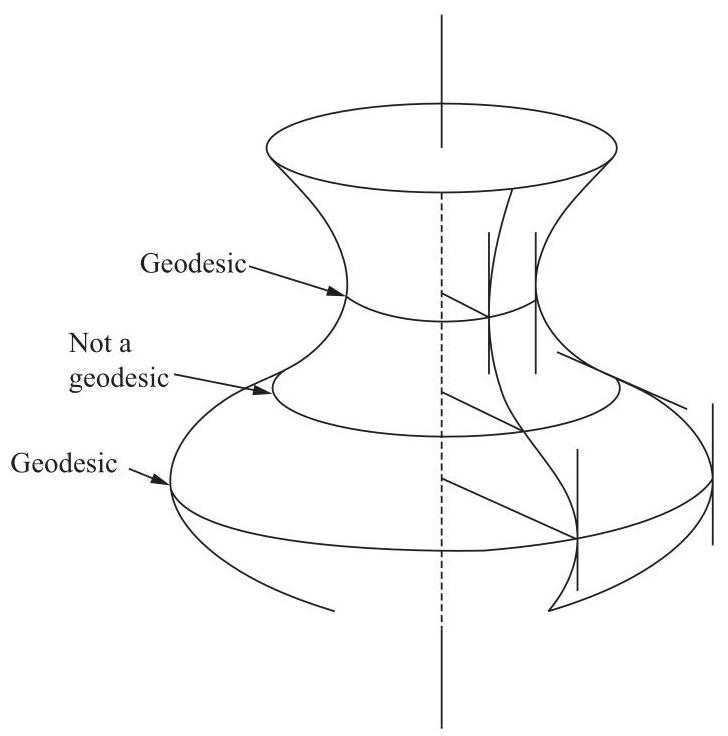
\includegraphics[max width=0.6\textwidth]{images/bo_d4b9jf3ef24c73e0334g_270_422_892_728_736_0.jpg}
\end{center}
\hspace*{3em} 

图 4-19

我们将从方程 (4a) 的第一个方程中得到一个有趣的几何推论，称为克莱罗关系.请注意，方程 (4a) 的第一个方程可以写成

\[
{\left( {f}^{2}{u}^{\prime }\right) }^{\prime } = {f}^{2}{u}^{\prime \prime } + {2f}{f}^{\prime }{u}^{\prime }{v}^{\prime } = 0;
\]

因此，

\[
{f}^{2}{u}^{\prime } = \text{ const. } = c.
\]

另一方面，测地线与相交的平行线的夹角 \(\theta ,0 \leq  \theta  \leq  \pi /2\) 由下式给出

\[
\cos \theta  = \frac{\left| \left\langle  {\mathbf{x}}_{u},{\mathbf{x}}_{u}{u}^{\prime } + {\mathbf{x}}_{v}{v}^{\prime }\right\rangle  \right| }{\left| {\mathbf{x}}_{u}\right| } = \left| {f{u}^{\prime }}\right| ,
\]

其中 \(\left\{  {{\mathbf{x}}_{u},{\mathbf{x}}_{v}}\right\}\) 是给定参数化相关的基.由于 \(f = r\) 是交点处平行线的半径，我们得到克莱罗关系:

\[
r\cos \theta  = \text{ const. } = \left| c\right| .
\]

在下一个例子中，我们将展示这个关系有多么有用.另请参阅练习 18、20 和 21.

最后，我们将证明方程组 (4a) 可以通过原函数进行积分.设 \(u = u\left( s\right) ,v = v\left( s\right)\) 为由弧长参数化的测地线，我们假设它既不是曲面的子午线也不是平行线.那么方程 (4a) 的第一个方程写为 \({f}^{2}{u}^{\prime } =\) const. \(= c \neq  0\) .

首先观察，沿 \(\left( {u\left( s\right) ,v\left( s\right) }\right)\) 的第一基本形式，

\[
1 = {f}^{2}{\left( \frac{du}{ds}\right) }^{2} + \left( {{\left( {f}^{\prime }\right) }^{2} + {\left( {g}^{\prime }\right) }^{2}}\right) {\left( \frac{dv}{ds}\right) }^{2}, \tag{5}
\]

与方程 (4a) 的第一个方程一起，等价于方程 (4a) 的第二个方程.事实上，通过将 \({f}^{2}{u}^{\prime } = c\) 代入方程 (5)，我们得到

\[
{\left( \frac{dv}{ds}\right) }^{2}\left( {{\left( {f}^{\prime }\right) }^{2} + {\left( {g}^{\prime }\right) }^{2}}\right)  =  - \frac{{c}^{2}}{{f}^{2}} + 1
\]

因此，通过对 \(s\) 求导，

\[
2\frac{dv}{ds}\frac{{d}^{2}v}{d{s}^{2}}\left( {{\left( {f}^{\prime }\right) }^{2} + {\left( {g}^{\prime }\right) }^{2}}\right)  + {\left( \frac{dv}{ds}\right) }^{2}\left( {2{f}^{\prime }{f}^{\prime \prime } + 2{g}^{\prime }{g}^{\prime \prime }}\right) \frac{dv}{ds} = \frac{{2f}{f}^{\prime }{c}^{2}}{{f}^{4}}\frac{dv}{ds},
\]

这等价于 (4a) 的第二个方程，因为 \(\left( {u\left( s\right) ,v\left( s\right) }\right)\) 不是平行圈.(当然，测地线可能与一个不是测地线的平行圈相切，这时 \({v}^{\prime }\left( s\right)  = 0\) .然而，Clairaut 关系表明这种情况只发生在孤立点).

另一方面，因为 \(c \neq  0\) (因为测地线不是子午线)，我们有 \({u}^{\prime }\left( s\right)  \neq  0\) .因此，我们可以反转 \(u = u\left( s\right)\) ，得到 \(s = s\left( u\right)\) ，从而得到 \(v = v\left( {s\left( u\right) }\right)\) .通过将方程 (5) 乘以 \({\left( ds/du\right) }^{2}\) ，我们得到

\[
{\left( \frac{ds}{du}\right) }^{2} = {f}^{2} + \left( {{\left( {f}^{\prime }\right) }^{2} + {\left( {g}^{\prime }\right) }^{2}}\right) {\left( \frac{dv}{ds}\frac{ds}{du}\right) }^{2},
\]

或者，利用 \({\left( ds/du\right) }^{2} = {f}^{4}/{c}^{2}\) 的事实，

\[
{f}^{2} = {c}^{2} + {c}^{2}\frac{{\left( {f}^{\prime }\right) }^{2} + {\left( {g}^{\prime }\right) }^{2}}{{f}^{2}}{\left( \frac{dv}{du}\right) }^{2},
\]

即，

\[
\frac{dv}{du} = \frac{1}{c}f\sqrt{\frac{{f}^{2} - {c}^{2}}{{\left( {f}^{\prime }\right) }^{2} + {\left( {g}^{\prime }\right) }^{2}}};
\]

因此，

\[
u = c\int \frac{1}{f}\sqrt{\frac{{\left( {f}^{\prime }\right) }^{2} + {\left( {g}^{\prime }\right) }^{2}}{{f}^{2} - {c}^{2}}}{dv} + \text{ const. } \tag{6}
\]

这是旋转曲面上既不是平行圈也不是子午线的测地线段的方程.

例 6.我们将证明，旋转抛物面 \(z = {x}^{2} + {y}^{2}\) 的任何非子午线的测地线都会与自身无限次相交.

设 \({p}_{0}\) 为抛物面上的一个点，设 \({P}_{0}\) 为通过 \({p}_{0}\) 的半径为 \({r}_{0}\) 的平行圈.设 \(\gamma\) 为通过 \({p}_{0}\) 且与 \({P}_{0}\) 成角 \({\theta }_{0}\) 的参数化测地线.因为根据 Clairaut 关系，

\[
r\cos \theta  = \text{ const. } = \left| c\right| ,\;0 \leq  \theta  \leq  \frac{\pi }{2},
\]

我们得出 \(\theta\) 随着 \(r\) 增大而增大.

因此，如果我们沿着平行圈增大的方向前进， \(\theta\) 就会增大.在某些旋转曲面上， \(\gamma\) 可能渐近地接近一条子午线.我们将在不久的将来证明旋转抛物面不是这种情况.也就是说，测地线 \(\gamma\) 与所有子午线相交，因此它绕抛物面旋转无限次.

另一方面，如果我们沿着平行圈减小的方向前进，角度 \(\theta\) 会减小并接近值 0，这对应于半径为 \(\left| c\right|\) 的平行圈 (注意，如果 \({\theta }_{0} \neq  0,\left| c\right|  < r\) ).我们将在本书后面证明，旋转曲面的任何测地线都不能渐近于一个不是测地线的平行圈 (第 4-7 节).由于抛物面的任何平行圈都不是测地线，因此测地线 \(\gamma\) 实际上在半径为 \(\left| c\right|\) 的平行圈上的点 \({p}_{1}\) 处相切.因为 1 是 \(\cos \theta\) 的最大值，所以 \(r\) 的值将从 \({p}_{1}\) 开始增加.因此，我们处于与之前相同的情况.测地线将围绕抛物面无限次旋转，朝着 \(r\) 增大的方向，并且它显然会与另一分支无限次相交 (图 4-20).

\begin{center}
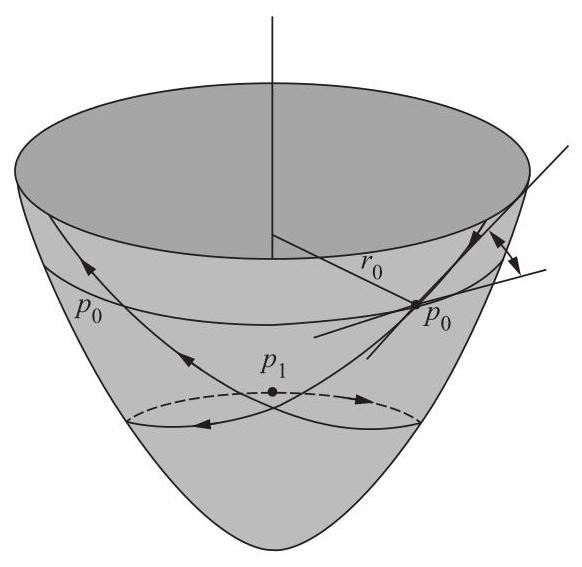
\includegraphics[max width=0.5\textwidth]{images/bo_d4b9jf3ef24c73e0334g_273_178_190_582_567_0.jpg}
\end{center}
\hspace*{3em} 

图 4-20

注意，如果 \({\theta }_{0} = 0\) ，初始情况是点 \({p}_{1}\) 的情况.

剩下要证明的是，当 \(r\) 增大时，测地线 \(\gamma\) 会遇到抛物面的所有子午线.最初注意，测地线不能与子午线相切.否则，根据命题 5 的唯一性部分，它将与子午线重合.因为角度 \(\theta\) 随着 \(r\) 增大而增大，如果 \(\gamma\) 没有与所有子午线相交，它将渐近地接近一条子午线，比如说 \(M\) .

我们假设情况如此，并为抛物面 \(z = {x}^{2} + {y}^{2}\) 选择一个局部坐标系，该坐标系由下式给出:

\[
x = v\cos u,\;y = v\sin u,\;z = {v}^{2},
\]

\[
0 < v <  + \infty ,\;0 < u < {2\pi },
\]

使得相应的坐标邻域包含 \(M\) 作为 \(u = {u}_{0}\) .根据假设，当 \(v \rightarrow  \infty\) 时，有 \(u \rightarrow  {u}_{0}\) .另一方面，该坐标系中测地线 \(y\) 的方程由(参见方程 (6))给出，示例 5，并选择 \(\gamma\) 上的一个方向，使得 \(c > 0\) )

\[
u = c\int \frac{1}{v}\sqrt{\frac{1 + 4{v}^{2}}{{v}^{2} - {c}^{2}}}{dv} + \text{ const. } > c\int \frac{dv}{v} + \text{ const. },
\]

因为

\[
\frac{1 + 4{v}^{2}}{{v}^{2} - {c}^{2}} > 1
\]

从上述不等式可以得出，当 \(v \rightarrow  \infty ,u\) 任意增大时，这与 \(\gamma\) 渐近于 \(M\) 的事实相矛盾.因此， \(\gamma\) 与所有经线相交，这就完成了本例开头所述论断的证明.

\exerciseline

1. a. 证明如果一条曲线 \(C \subset  S\) 既是曲率线又是测地线，那么 \(C\) 是平面曲线.

b. 证明如果一条(非直线)测地线是平面曲线，那么它是一条曲率线.

c. 举一个曲率线是平面曲线但不是测地线的例子.

2. 证明曲线 \(C \subset  S\) 既是渐近线又是测地线，当且仅当 \(C\) 是(一段)直线.

3. 不使用命题 5，证明直线是平面上唯一的测地线.

4. 设 \(v\) 和 \(w\) 是曲线 \(\alpha  : I \rightarrow  S\) 上的向量场.证明

\[
\frac{d}{dt}\langle v\left( t\right) ,w\left( t\right) \rangle  = \left\langle  {\frac{Dv}{dt},w\left( t\right) }\right\rangle   + \left\langle  {v\left( t\right) ,\frac{Dw}{dt}}\right\rangle  .
\]

5. 考虑由旋转圆生成的旋转环面

\[
{\left( x - a\right) }^{2} + {z}^{2} = {r}^{2},y = 0,
\]

绕 \(z\) 轴 \(\left( {a > r > 0}\right)\) .由 \(\left( {a + r,0}\right) ,\left( {a - r,0}\right) ,\left( {a,r}\right)\) 点生成的平行线分别称为最大平行线、最小平行线和上平行线.检查这些平行线中的哪一条是

a. 测地线.

b. 渐近线.

c. 曲率线.

*6. 计算练习5中圆环的上平行线的测地曲率.

7. 将圆柱面 \({x}^{2} + {y}^{2} = 1\) 与一条通过 \(x\) 轴且与 \({xy}\) 平面成 \(\theta ,0 < \theta  < \pi /2\) 角的平面相交.

a. 证明交线是一个椭圆 \(C\) .

b. 计算 \(C\) 在圆柱面上与其主轴相交点的测地曲率的绝对值.

*8. 证明如果一个连通曲面的所有测地线都是平面曲线，则该曲面包含在一个平面或一个球体中.

*9. 考虑一个球面 \({C}_{1}\) 和 \({C}_{2}\) 的两条经线，它们在点 \({p}_{1}\) 处成角 \(\varphi\) .沿着 \({C}_{1}\) 和 \({C}_{2}\) ，从初始点 \({p}_{1}\) 到两条经线再次相遇的点 \({p}_{2}\) ，平行移动 \({C}_{1}\) 的切向量 \({w}_{0}\) ，分别得到 \({w}_{1}\) 和 \({w}_{2}\) .计算从 \({w}_{1}\) 到 \({w}_{2}\) 的角度.

*10. 证明一个定向曲线 \(C \subset  S\) 在点 \(p \in  C\) 的测地曲率等于将 \(C\) 沿着曲面在 \(p\) 处的法线投影到切平面 \({T}_{p}\left( S\right)\) 上得到的平面曲线的曲率.

11. 精确陈述并证明:协变导数的代数值在保持方向的等距变换下不变.

*12. 我们说曲面 \(S\) 上的一组正则曲线是 \(S\) 上的可微曲线族，如果该族曲线的切线构成一个可微方向场(参见第3-4节).假设曲面 \(S\) 存在两条可微的正交测地线族.证明 \(S\) 的高斯曲率为零.

*13. 令 \(V\) 为曲面 \(S\) 上一点 \(p\) 的一个连通邻域，并假设 \(V\) 中任意两点之间的平行移动不依赖于连接这两点的曲线.证明 \(V\) 的高斯曲率为零.

14. 令 \(S\) 为一个定向正则曲面，令 \(\alpha  : I \rightarrow  S\) 为一条由弧长参数化的曲线.在点 \(p = \alpha \left( s\right)\) 处考虑三个单位向量(达布三面体) \(T\left( s\right)  = {\alpha }^{\prime }\left( s\right) ,N\left( s\right)  =\) 曲面在 \(p,V\left( s\right)  = N\left( s\right)  \land  T\left( s\right)\) 处的法向量.证明

\[
\frac{dT}{ds} = 0 + {aV} + {bN}
\]

\[
\frac{dV}{ds} =  - {aT} + 0 + {cN},
\]

\[
\frac{dN}{ds} =  - {bT} - {cV} + 0,
\]

其中 \(a = a\left( s\right) ,b = b\left( s\right) ,c = c\left( s\right) ,s \in  I\) .上述公式是三面体 \(T,V,N\) 的弗雷内公式的类似物.为了确定系数的几何意义，证明

a. \(c =  - \langle {dN}/{ds},V\rangle\) ；由此得出，当且仅当 \(c \equiv  0( - c\) 是 \(\alpha\) 的测地挠率时， \(\alpha \left( I\right)  \subset  S\) 是一条曲率线(参见第3-2节练习19).

b. \(b\) 是 \(\alpha \left( I\right)  \subset  S\) 在 \(p\) 处的法曲率.

c. \(a\) 是 \(\alpha \left( I\right)  \subset  S\) 在 \(p\) 处的测地曲率.

设 \({p}_{0}\) 为单位球面 \({S}^{2}\) 的极点，设 \(q,r\) 为对应赤道上的两点，使得子午线 \({p}_{0}q\) 和 \({p}_{0}r\) 在 \({p}_{0}\) 处夹角为 \(\theta\) .考虑一个单位向量 \(v\) ，它在 \({p}_{0}\) 处与子午线 \({p}_{0}q\) 相切，并将 \(v\) 沿着由子午线 \({p}_{0}q\) 、纬线 \({qr}\) 和子午线 \(r{p}_{0}\) 组成的闭合曲线进行平行移动(图 4-21).

\begin{center}
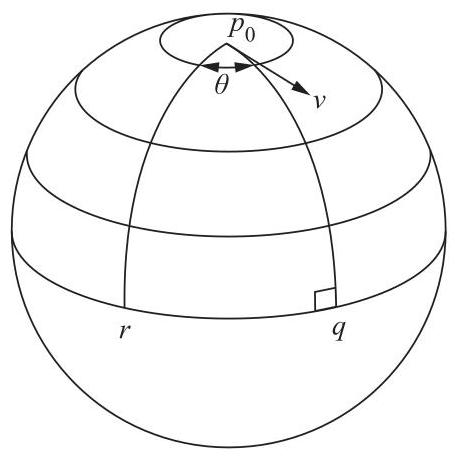
\includegraphics[max width=0.4\textwidth]{images/bo_d4b9jf3ef24c73e0334g_276_198_199_455_459_0.jpg}
\end{center}
\hspace*{3em} 

图 4-21

a. 求 \(v\) 的最终位置与 \(v\) 之间的夹角.

b. 当点 \(r,q\) 不在赤道上，而是在余纬 \(\varphi\) 的平行圈上时，执行相同的操作(参见示例 1).

*16. 设 \(p\) 是一个定向曲面 \(S\) 上的点，并假设在 \(p\) 的一个邻域内， \(S\) 上的所有点都是抛物点.证明通过 \(p\) 的(唯一)渐近线是一条直线段.举例说明具有抛物点邻域的条件是必不可少的.

17. 设 \(\alpha  : I \rightarrow  {R}^{3}\) 是由弧长 \(s\) 参数化的曲线，其曲率和挠率均不为零.考虑参数化曲面(第 2-3 节)

\[
\mathbf{x}\left( {s,v}\right)  = \alpha \left( s\right)  + {vb}\left( s\right) ,\;s \in  I, - \epsilon  < v < \epsilon ,\epsilon  > 0,
\]

其中 \(b\) 是 \(\alpha\) 的副法向量.证明如果 \(\epsilon\) 很小，则 \(\mathbf{x}(I \times \; \left( {-\epsilon ,\epsilon }\right) ) = S\) 是一个正则曲面，其上 \(\alpha \left( I\right)\) 是测地线(因此，每条曲线都是由其副法线生成的曲面上的测地线).

*18. 考虑一条测地线，它从双曲面 \({x}^{2} + {y}^{2} - {z}^{2} = 1\) 的上半部分 \(\left( {z > 0}\right)\) 中的点 \(p\) 开始，并与通过 \(p\) 的平行圈成角 \(\theta\) ，使得 \(\cos \theta  = 1/r\) ，其中 \(r\) 是 \(p\) 到 \(z\) 轴的距离.证明通过沿着测地线朝减小平行圈的方向前进，它渐近地接近平行圈 \({x}^{2} + {y}^{2} = 1,z = 0\) (图 4-22).

*19. 证明当测地线的微分方程(4)参照弧长时，方程(4)的第二个方程除了坐标曲线外，是方程(4)的第一个方程的推论.

*20. 设 \(T\) 是一个旋转环面，我们将假设它由(参见示例 6，第 2-2 节)参数化

\[
\mathbf{x}\left( {u,v}\right)  = \left( {\left( {r\cos u + a}\right) \cos v,\left( {r\cos u + a}\right) \sin v,r\sin u}\right) .
\]

\begin{center}
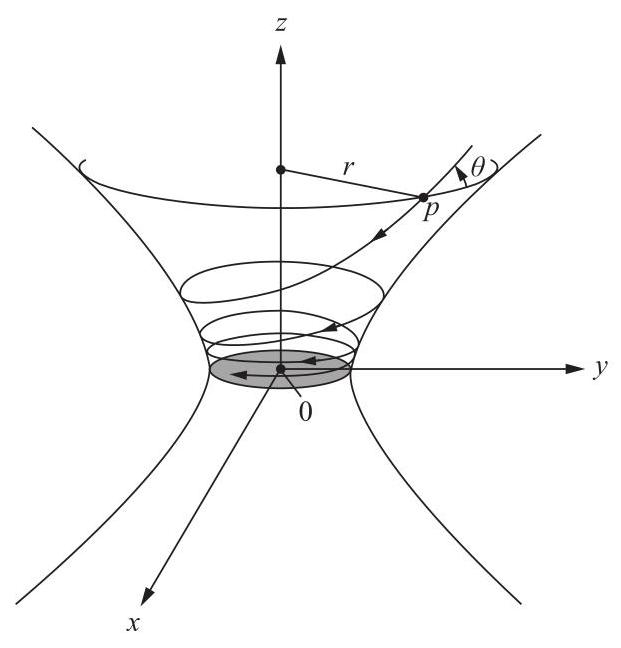
\includegraphics[max width=0.5\textwidth]{images/bo_d4b9jf3ef24c73e0334g_277_177_199_621_648_0.jpg}
\end{center}
\hspace*{3em} 

图 4-22

证明

a. 如果一条测地线与平行圈 \(u = \pi /2\) 相切，则它完全包含在 \(T\) 的区域中，该区域由下式给出:

\[
- \frac{\pi }{2} \leq  u \leq  \frac{\pi }{2}.
\]

b. 一条与平行圈 \(u = 0\) 成角 \(\theta \; \left( {0 < \theta  < \pi /2}\right)\) 相交的测地线也与平行圈 \(u = \pi\) 相交，如果

\[
\cos \theta  < \frac{a - r}{a + r}
\]

21. 黎曼曲面是那些可以得到一组局部坐标 \(\mathbf{x}\left( {u,v}\right)\) 的曲面，使得第一基本形式的系数可以写成如下形式:

\[
E = G = U + V,\;F = 0,
\]

其中 \(U = U\left( u\right)\) 仅是 \(u\) 的函数，而 \(V = V\left( v\right)\) 仅是 \(v\) 的函数.请注意，黎曼曲面是旋转曲面的推广，并证明(参见示例 5)

a. 黎曼曲面的测地线可以通过积分得到，形式为:

\[
\int \frac{du}{\sqrt{U - c}} =  \pm  \int \frac{dv}{\sqrt{V + c}} + {c}_{1}
\]

其中 \(c\) 和 \({c}_{1}\) 是取决于初始条件的常数.

b. 如果 \(\theta ,0 \leq  \theta  \leq  \pi /2\) 是测地线与曲线 \(v =\) const. 所成的角度，则

\[
U{\sin }^{2}\theta  - V{\cos }^{2}\theta  = \text{ const. }
\]

(请注意，这是 Liouville 曲面 Clairaut 关系的类似物.)

22. 令 \({S}^{2} = \left\{  {\left( {x,y,z}\right)  \in  {R}^{3};{x}^{2} + {y}^{2} + {z}^{2} = 1}\right\}\) 且令 \(p \in  {S}^{2}\) .对于每条分段正则参数化曲线 \(\alpha  : \left\lbrack  {0,l}\right\rbrack   \rightarrow  {S}^{2}\) 且满足 \(\alpha \left( 0\right)  = \alpha \left( l\right)  = \; p\) ，令 \({P}_{\alpha } : {T}_{p}\left( {S}^{2}\right)  \rightarrow  {T}_{p}\left( {S}^{2}\right)\) 为将每一点 \(v \in \; {T}_{p}\left( {S}^{2}\right)\) 沿 \(\alpha\) 平行移动回 \(p\) 的映射.根据命题 1， \({P}_{\alpha }\) 是一个等距映射.证明对于 \({T}_{p}\left( S\right)\) 的每一次旋转 \(R\) ，都存在一个 \(\alpha\) 使得 \(R = {P}_{\alpha }\) .

23. 证明单位球面的等距映射

\[
{S}^{2} = \left\{  {\left( {x,y,z}\right)  \in  {R}^{3};{x}^{2} + {y}^{2} + {z}^{2} = 1}\right\}
\]

是 \({R}^{3}\) 的线性正交变换在 \({S}^{2}\) 上的限制.

\section*{4-5. 高斯-博内定理及其应用}

在本节中，我们将介绍高斯-博内定理及其一些推论.该定理涉及的几何学相当简单，其证明的难点在于某些拓扑事实.这些事实将不加证明地呈现.

高斯-博内定理可能是曲面微分几何中最深刻的定理.该定理的一个早期版本由高斯在一个著名的论文 [1] 中提出，涉及曲面上的测地三角形(即边是测地线弧的三角形).粗略地说，它断言一个测地三角形 \(T\) 的内角和 \({\varphi }_{1},{\varphi }_{2},{\varphi }_{3}\) 超过 \(\pi\) 的量等于高斯曲率 \(K\) 在 \(T\) 上的积分；即(图 4-23)，

\[
\mathop{\sum }\limits_{{i = 1}}^{3}{\varphi }_{i} - \pi  = {\iint }_{T}{Kd\sigma }
\]

例如，如果 \(K \equiv  0\) ，我们得到 \(\sum {\varphi }_{i} = \pi\) ，这是高中几何中 Thales 定理在零曲率曲面上的推广.同样，如果 \(K \equiv  1\) ，我们得到 \(\sum {\varphi }_{i} - \pi  = \operatorname{area}\left( T\right)  > 0\) .因此，在单位球面上，任何测地三角形的内角和都大于 \(\pi\) ，而超过 \(\pi\) 的量恰好是 \(T\) 的面积.类似地，在伪球面(练习 6，第 3-3 节)上，任何测地三角形的内角和都小于 \(\pi\) (图 4-24).

\begin{center}
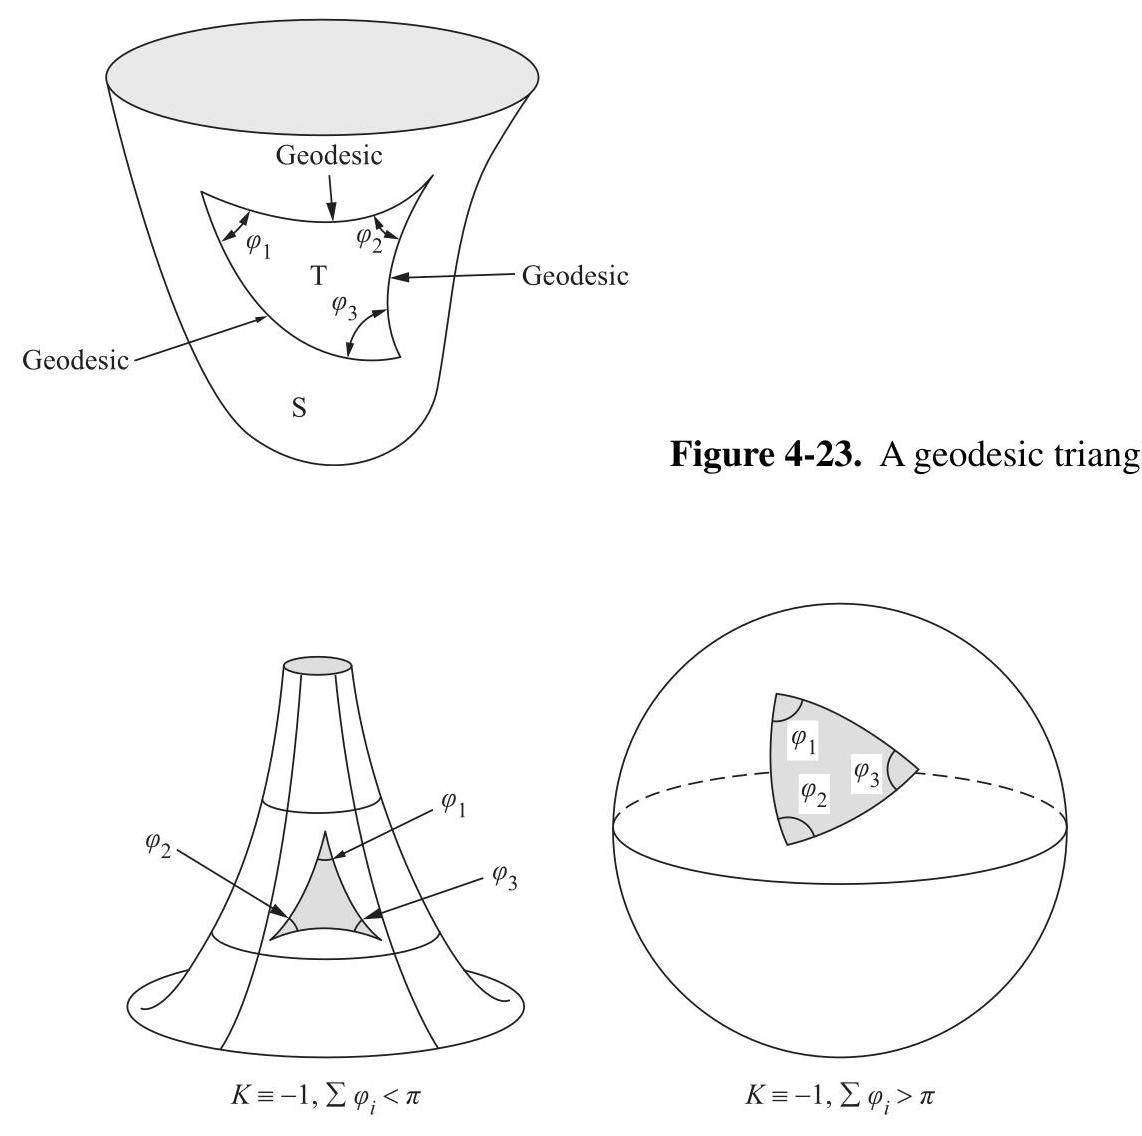
\includegraphics[max width=1.0\textwidth]{images/bo_d4b9jf3ef24c73e0334g_279_170_185_1142_1136_0.jpg}
\end{center}
\hspace*{3em} 

图 4-24

该定理推广到由非测地简单曲线(见下文公式 (1))所界定的区域，归功于 O. Bonnet.为了进一步推广它，例如推广到紧致曲面，将涉及一些拓扑学的考虑.实际上，高斯-博内定理最重要的特征之一是它在紧致曲面的拓扑与其曲率积分之间提供了一个 remarkable 的关系(见下文推论 2).

现在我们将开始介绍高斯-博内定理局部版本的一些细节.我们需要一些定义.

设 \(\alpha  : \left\lbrack  {0,l}\right\rbrack   \rightarrow  S\) 是从闭区间 \(\left\lbrack  {0,l}\right\rbrack\) 到正则曲面 \(S\) 的连续映射.我们称 \(\alpha\) 是一个简单、闭合、分段正则的参数化曲线，如果

1. \(\alpha \left( 0\right)  = \alpha \left( l\right)\) .

2. \({t}_{1} \neq  {t}_{2},{t}_{1},{t}_{2} \in  \lbrack 0,l)\) ，意味着 \(\alpha \left( {t}_{1}\right)  \neq  \alpha \left( {t}_{2}\right)\) .

3. 存在一个细分

\[
0 = {t}_{0} < {t}_{1} < \cdots  < {t}_{k} < {t}_{k + 1} = l
\]

使得 \(\alpha\) 在每个 \(\left( {{t}_{i},{t}_{i + 1}}\right) ,i = \; 0,\ldots ,k\) 中可微且正则的 \((0,l\rbrack\) .

直观地说，这意味着 \(\alpha\) 是一条闭合曲线(条件 1)，没有自交点(条件 2)，并且只在有限个点处无法定义切线(条件 3).

点 \(\alpha \left( {t}_{i}\right) ,i = 0,\ldots ,k\) 称为 \(\alpha\) 的顶点，而轨迹 \(\alpha \left( \left\lbrack  {{t}_{i},{t}_{i + 1}}\right\rbrack  \right)\) 称为 \(\alpha\) 的正则弧.通常称轨迹 \(\alpha \left( \left\lbrack  {0,l}\right\rbrack  \right)\) 为闭合分段正则曲线.

根据正则性条件，对于每个顶点 \(\alpha \left( {t}_{i}\right)\) ，存在左极限，即对于 \(t < {t}_{i}\)

\[
\mathop{\lim }\limits_{{t \rightarrow  {t}_{i}}}{\alpha }^{\prime }\left( t\right)  = {\alpha }^{\prime }\left( {{t}_{i} - 0}\right)  \neq  0,
\]

和右极限，即对于 \(t > {t}_{i}\) ，

\[
\mathop{\lim }\limits_{{t \rightarrow  {t}_{i}}}{\alpha }^{\prime }\left( t\right)  = {\alpha }^{\prime }\left( {{t}_{i} + 0}\right)  \neq  0.
\]

现在假设 \(S\) 是定向的，设 \(\left| {\theta }_{i}\right| ,0 \leq  \left| {\theta }_{i}\right|  < \pi\) 是从 \({\alpha }^{\prime }\left( {{t}_{i} - 0}\right)\) 到 \({\alpha }^{\prime }\left( {{t}_{i} + 0}\right)\) 的角度的最小确定值.如果 \(\left| {\theta }_{i}\right|  \neq  \pi\) ，我们赋予 \({\theta }_{i}\) 行列式 \(\left( {{\alpha }^{\prime }\left( {{t}_{i} - 0}\right) ,{\alpha }^{\prime }\left( {{t}_{i} + 0}\right) ,N}\right)\) 的符号.这意味着如果顶点 \(\alpha \left( {t}_{i}\right)\) 不是一个“尖点”(图 4-25)，则 \({\theta }_{i}\) 的符号由 \(S\) 的定向给出.有符号角 \({\theta }_{i}, - \pi  < {\theta }_{i} < \pi\) 称为顶点 \(\alpha \left( {t}_{i}\right)\) 处的外角.

在 \(\alpha \left( {t}_{i}\right)\) 是尖点的情况下，即 \(\left| {\theta }_{i}\right|  = \pi\) ，我们按如下方式选择 \({\theta }_{i}\) 的符号.设闭合简单曲线 \(\alpha\) 包含在具有给定方向的共形参数化图像中，并假设 \(\alpha \left( {t}_{i}\right)\) 是一个尖点.选择坐标轴 \({x0y}\) ，其中 \(\alpha \left( {t}_{i}\right)  = 0\) ，具有给定的方向，并进一步假设 \(\alpha\) 到达 \(\alpha \left( {t}_{i}\right)\) 的部分指向轴 \({0x}\) 的负方向(当然， \(\alpha\) 离开 \(\alpha \left( {t}_{i}\right)\) 的部分指向轴 \({0x})\) 的正方向).

\begin{center}
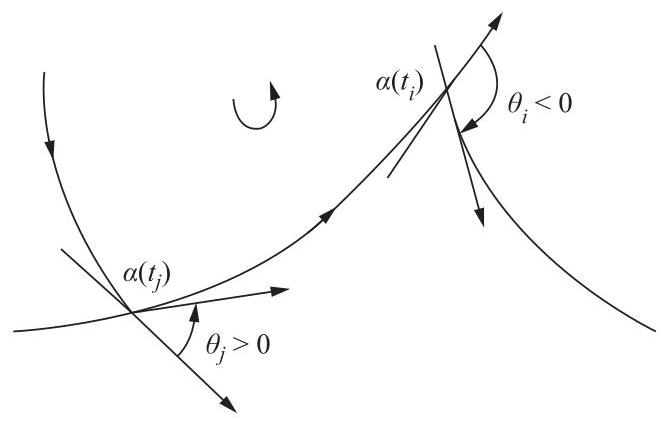
\includegraphics[max width=0.6\textwidth]{images/bo_d4b9jf3ef24c73e0334g_280_448_1622_667_422_0.jpg}
\end{center}
\hspace*{3em} 

图 4-25

\begin{center}
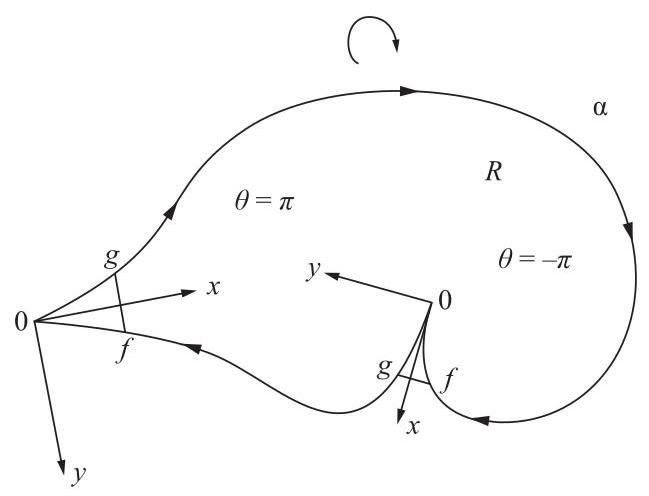
\includegraphics[max width=0.5\textwidth]{images/bo_d4b9jf3ef24c73e0334g_281_448_191_649_496_0.jpg}
\end{center}
\hspace*{3em} 

图 4-26. 尖点情况下的外角符号.

对于小的 \(\varepsilon  > 0\) ，到达 \(\alpha \left( {t}_{i}\right)\) 附近的 \(\alpha\) 的部分由函数 \(f\left( x\right)  = y,0 < x < \epsilon\) 给出，而离开 \({t}_{i}\) 附近的 \(\alpha\) 的部分由函数 \(g\left( x\right)  = y,0 < x < \epsilon\) 给出.如果 \(f > 0\) 和 \(g < 0\) ，我们设 \(\theta \left( {t}_{i}\right)  = \pi\) ；如果 \(f < 0\) 和 \(g > 0\) ，我们设 \(\theta \left( {t}_{i}\right)  =  - \pi\) .

这就解决了尖点处角度的问题.

设 \(\alpha  : \left\lbrack  {0,l}\right\rbrack   \rightarrow  \mathbf{x}\left( U\right)  \subset  S\) 为一条简单的闭合、分段正则、参数化的曲线，其顶点为 \(\alpha \left( {t}_{i}\right)\) ，外角为 \({\theta }_{i},i = 0,\ldots ,k\) .

设 \({\varphi }_{i} : \left\lbrack  {{t}_{i},{t}_{i + 1}}\right\rbrack   \rightarrow  R\) 为可微函数，它们在每个 \(t \in  \left\lbrack  {{t}_{i},{t}_{i + 1}}\right\rbrack\) 处测量从 \({\mathbf{x}}_{u}\) 到 \({\alpha }^{\prime }\left( t\right)\) 的正角(参见引理 1，第 4-4 节).

我们将要提出的第一个拓扑事实是以下内容，不加证明.

定理(转切线定理).在上述记号下，对于平面曲线，我们有

\[
\mathop{\sum }\limits_{{\mathrm{i} = 0}}^{\mathrm{k}}\left( {{\varphi }_{\mathrm{i}}\left( {\mathrm{t}}_{\mathrm{i} + 1}\right)  - {\varphi }_{\mathrm{i}}\left( {\mathrm{t}}_{\mathrm{i}}\right) }\right)  + \mathop{\sum }\limits_{{\mathrm{i} = 0}}^{\mathrm{k}}{\theta }_{\mathrm{i}} =  \pm  {2\pi },
\]

其中加号或减号取决于 \(\alpha\) 的方向.

该定理指出，切线向量对 \(\alpha\) 的角度的总变化量加上顶点处的“跳跃”等于 \({2\pi }\) .

H. Hopf 在 Compositio Math. 2 (1935), 50-62 给出该定理的一个优雅证明.对于 \(\alpha\) 没有顶点的 경우，Hopf 的证明可以在本书第 5-7 节(定理 2)中找到.应该注意的是，Hopf 的证明是针对平面曲线的.

在陈述高斯-博内定理的局部版本之前，我们还需要一些术语.

令 \(S\) 为一个定向曲面.一个区域 \(R \subset  S\) (一个连通开集与其边界的并集)称为简单区域，如果 \(R\) 与一个圆盘同胚，并且 \(R\) 的边界 \(\partial R\) 是一个简单、闭合、分段正则的参数化曲线 \(\alpha  : I \rightarrow  S\) 的轨迹.我们称 \(\alpha\) 是正定向的，如果对于每个属于正则弧的 \(\alpha \left( t\right)\) ，正交基 \(\left\{  {{\alpha }^{\prime }\left( t\right) ,h\left( t\right) }\right\}\) 满足 \(h\left( t\right)\) “指向” \(R\) ；更精确地说，对于任何具有 \(\beta \left( 0\right)  = \alpha \left( t\right)\) 和 \({\beta }^{\prime }\left( 0\right)  \neq  {\alpha }^{\prime }\left( t\right)\) 的曲线 \(\beta  : I \rightarrow  R\) ，我们有 \(\left\langle  {{\beta }^{\prime }\left( 0\right) ,h\left( t\right) }\right\rangle   > 0\) .直观地说，这意味着如果一个人沿着曲线 \(\alpha\) 朝正方向行走，头部指向 \(N\) ，那么区域 \(R\) 就会留在左侧(图 4-27).可以证明， \(\alpha\) 的两种可能定向中的一种使其成为正定向.

\begin{center}
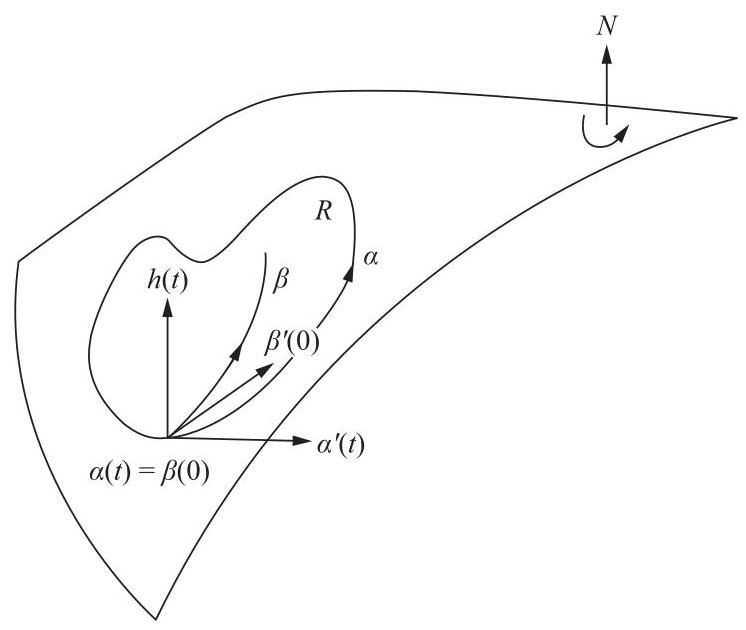
\includegraphics[max width=0.6\textwidth]{images/bo_d4b9jf3ef24c73e0334g_282_409_787_746_630_0.jpg}
\end{center}
\hspace*{3em} 

图 4-27. 一个正定向的边界曲线.

现在令 \(\mathbf{x} : U \subset  {R}^{2} \rightarrow  S\) 为与 \(S\) 的定向兼容的 \(S\) 的一个参数化，并令 \(R \subset  \mathbf{x}\left( U\right)\) 为 \(S\) 的一个有界区域.如果 \(f\) 是 \(S\) 上的一个可微函数，那么很容易看出积分

\[
{\iint }_{{\mathbf{x}}^{-1}\left( R\right) }f\left( {u,v}\right) \sqrt{{EG} - {F}^{2}}{dudv}
\]

不依赖于在 \(\mathbf{x}\) 的定向类别中选择的参数化 \(\mathbf{x}\) .(证明与面积定义中的相同；参见第 2-5 节.)因此，这个积分具有几何意义，称为 \(f\) 在区域 \(R\) 上的积分.通常用

\[
{\iint }_{R}{fd\sigma }
\]

用这些定义，我们现在陈述

高斯-博内定理(局部).令 \(\mathbf{x} : \mathrm{U} \rightarrow  S\) 为一个定向曲面 \(S\) 的等温参数化(即， \(F = 0,E = G = {\lambda }^{2}\left( {u,v}\right)\) ).参见第 4.2 节，命题 2 之后)其中 \(\mathrm{U} \subset  {\mathbb{R}}^{2}\) 与一个开圆盘同胚，并且 \(\mathbf{x}\) 与 \(S\) 的定向兼容.

令 \(\mathbb{R} \subset  \mathbf{x}\left( \mathrm{U}\right)\) 为 \(S\) 的一个简单区域，并令 \(\alpha  : I \rightarrow  S\) 使得 \(\partial \mathbb{R} = \alpha \left( \mathrm{I}\right)\) .假设 \(\alpha\) 是正定向的，由弧长 \(S\) 参数化，并令 \(\alpha \left( {S}_{0}\right) ,\ldots ,\alpha \left( {S}_{\mathrm{k}}\right)\) 和 \({\theta }_{0},\ldots ,{\theta }_{\mathrm{k}}\) 分别为 \(\alpha\) 的顶点和外角.则

\[
\mathop{\sum }\limits_{{\mathrm{i} = 0}}^{\mathrm{k}}{\int }_{{S}_{\mathrm{i}}}^{{S}_{\mathrm{i} + 1}}{\mathrm{k}}_{\mathrm{g}}\left( S\right) \mathrm{{ds}} + {\iint }_{\mathbb{R}}\mathrm{K}\mathrm{d}\sigma  + \mathop{\sum }\limits_{{\mathrm{i} = 0}}^{\mathrm{k}}{\theta }_{\mathrm{i}} = {2\pi }, \tag{1}
\]

其中 \({\mathrm{k}}_{\mathrm{g}}\left( S\right)\) 是 \(\alpha\) 的正则弧的测地曲率，而 \(\mathrm{K}\) 是 \(S\) 的高斯曲率.

注. 区域 \(R\) 包含在等温参数化图像集中的限制仅是为了简化证明并能使用转切线定理. 正如我们稍后将看到的 (全局高斯-博内定理的推论 1)，上述结果对于正则曲面上的任何简单区域仍然成立. 这是非常合理的，因为方程 (1) 并不以任何方式涉及特定的参数化. \({}^{ \dagger  }\)

证明. 令 \(u = u\left( s\right) ,v = v\left( s\right)\) 为 \(\alpha\) 在参数化 \(\mathbf{x}\) 下的表达式. 使用 4-4 节的命题 3，我们得到

\[
{k}_{g}\left( s\right)  = \frac{1}{2\sqrt{EG}}\left\{  {{G}_{u}\frac{dv}{ds} - {E}_{v}\frac{du}{ds}}\right\}   + \frac{d{\varphi }_{i}}{ds},
\]

其中 \({\varphi }_{i} = {\varphi }_{i}\left( s\right)\) 是一个可微函数，它测量了 \({\mathbf{x}}_{u}\) 到 \({\alpha }^{\prime }\left( s\right)\) 在 \(\left\lbrack  {{s}_{i},{s}_{i + 1}}\right\rbrack\) 中的正角. 通过在每个区间 \(\left\lbrack  {{s}_{i},{s}_{i + 1}}\right\rbrack\) 上积分上述表达式并将结果相加，

\[
\mathop{\sum }\limits_{{i = 0}}^{k}{\int }_{{s}_{i}}^{{s}_{i + 1}}{k}_{g}\left( s\right) {ds} = \mathop{\sum }\limits_{{i = 0}}^{k}{\int }_{{s}_{i}}^{{s}_{i + 1}}\left( {\frac{{G}_{u}}{2\sqrt{EG}}\frac{dv}{ds} - \frac{{E}_{v}}{2\sqrt{EG}}\frac{du}{ds}}\right) {ds}
\]

\[
+ \mathop{\sum }\limits_{{i = 0}}^{k}{\int }_{{s}_{i}}^{{s}_{i + 1}}\frac{d{\varphi }_{i}}{ds}{ds}
\]

现在我们使用 \({uv}\) 平面上的高斯-格林定理，该定理说明如下: 如果 \(P\left( {u,v}\right)\) 和 \(Q\left( {u,v}\right)\) 是简单区域 \(A \subset  {R}^{2}\) 中的可微函数，其边界由 \(u = u\left( s\right) ,v = v\left( s\right)\) 给出，则

\[
\mathop{\sum }\limits_{{i = 0}}^{k}{\int }_{{s}_{i}}^{{s}_{i + 1}}\left( {P\frac{du}{ds} + Q\frac{dv}{ds}}\right) {ds} = {\iint }_{A}\left( {\frac{\partial Q}{\partial u} - \frac{\partial P}{\partial v}}\right) {dudv}.
\]



†如果此断言为真，则下面给出的应用 2 和 6 即可呈现.



由此得出

\[
\mathop{\sum }\limits_{{i = 0}}^{k}{\int }_{{s}_{i}}^{{s}_{i + 1}}{k}_{g}\left( s\right) {ds} = {\iint }_{{\mathbf{x}}^{-1\left( R\right) }}\left\{  {{\left( \frac{{E}_{v}}{2\sqrt{EG}}\right) }_{v} + {\left( \frac{{G}_{u}}{2\sqrt{EG}}\right) }_{u}}\right\}  {dudv}
\]

\[
+ \mathop{\sum }\limits_{{i = 0}}^{k}{\int }_{{s}_{i}}^{{s}_{i + 1}}\frac{d{\varphi }_{i}}{ds}{ds}
\]

为了能够使用转切线定理，我们必须假设我们的参数化是等温的，也就是说，除了 \(F = 0\) 之外，我们还有 \(E = G = \lambda \left( {u,v}\right)  > 0\) . 在这种情况下，

\[
{\left( \frac{{E}_{v}}{2\sqrt{EG}}\right) }_{v} + {\left( \frac{{G}_{u}}{2\sqrt{EG}}\right) }_{u} = \frac{1}{2}\left\{  {{\left( \frac{{\lambda }_{v}}{\lambda }\right) }_{v} + {\left( \frac{{\lambda }_{u}}{\lambda }\right) }_{u}}\right\}
\]

\[
= \frac{1}{2\lambda }\left\{  {{\left( \log \lambda \right) }_{vv} + {\left( \log \lambda \right) }_{uu}}\right\}  \lambda
\]

\[
= \frac{1}{2\lambda }\left( {\Delta \log \lambda }\right) \lambda  =  - {K\lambda },
\]

在最后一个等式中，我们使用了 4-3 节的练习 2. 通过在坐标邻域的定义域上积分上述表达式，我们得到

\[
\mathop{\sum }\limits_{{i = 0}}^{k}{\int }_{{s}_{i}}^{{s}_{i + 1}}{k}_{g}\left( s\right) {ds} =  - {\iint }_{R}{K\lambda dudv} + \mathop{\sum }\limits_{i}{\int }_{{s}_{i}}^{{s}_{i + 1}}\frac{d{\varphi }_{i}}{ds}{ds}
\]

另一方面，根据转切线定理，

\[
\mathop{\sum }\limits_{{i = 0}}^{k}{\int }_{{s}_{i}}^{{s}_{i + 1}}\frac{d{\varphi }_{i}}{ds}{ds} = \mathop{\sum }\limits_{{i = 0}}^{k}\left( {{\varphi }_{i}\left( {s}_{i + 1}\right)  - {\varphi }_{i}\left( {s}_{i}\right) }\right)
\]

\[
=  \pm  {2\pi } - \mathop{\sum }\limits_{{i = 0}}^{k}{\theta }_{i}
\]

由于曲线 \(\alpha\) 是正向定向的，符号应该是加号，正如在平面圆的特例中可以轻易看到的.

将这些事实结合起来，我们得到

\[
\mathop{\sum }\limits_{{i = 0}}^{k}{\int }_{{s}_{i}}^{{s}_{i + 1}}{k}_{g}\left( s\right) {ds} + {\iint }_{R}{Kd\sigma } + \mathop{\sum }\limits_{{i = 0}}^{k}{\theta }_{i} = {2\pi }. \tag{Q.E.D.}
\]

在进入高斯-博内定理的全局版本之前，我们想展示该定理证明中使用的技术如何也可能用于解释高斯曲率与平行性的关系.

为此，令 \(\mathbf{x} : U \rightarrow  S\) 是某点 \(p \in  S\) 处的等温参数化，令 \(R \subset  \mathbf{x}\left( U\right)\) 是一个不含顶点的简单区域，其中包含 \(p\) 在其内部. 令 \(\alpha  : \left\lbrack  {0,l}\right\rbrack   \rightarrow  \mathbf{x}\left( U\right)\) 为由弧长 \(s\) 参数化的曲线，使得 \(\alpha\) 的轨迹是 \(R\) 的边界. 令 \({w}_{0}\) 为切向 \(S\) 在 \(\alpha \left( 0\right)\) 处的单位向量，令 \(w\left( s\right) ,s \in  \left\lbrack  {0,l}\right\rbrack\) 为 \({w}_{0}\) 沿 \(\alpha\) 的平行移动 (图 4-28). 使用 4-4 节的命题 3 和 \({uv}\) 平面上的高斯-格林定理，我们得到

\[
0 = {\int }_{0}^{l}\left\lbrack  \frac{Dw}{ds}\right\rbrack  {ds}
\]

\[
= {\int }_{0}^{l}\frac{1}{2\sqrt{EG}}\left\{  {{G}_{u}\frac{dv}{ds} - {E}_{v}\frac{du}{ds}}\right\}  {ds} + {\int }_{0}^{l}\frac{d\varphi }{ds}{ds}
\]

\[
=  - {\iint }_{R}{Kd\sigma } + \varphi \left( l\right)  - \varphi \left( 0\right) ,
\]

其中 \(\varphi  = \varphi \left( s\right)\) 是从 \({\mathbf{x}}_{u}\) 到 \(w\left( s\right)\) 的角度的一个可微确定值. 由此得出 \(\varphi \left( l\right)  - \varphi \left( 0\right)  = {\Delta \varphi }\) 由下式给出

\[
{\Delta \varphi } = {\iint }_{R}{Kd\sigma } \tag{2}
\]

\begin{center}
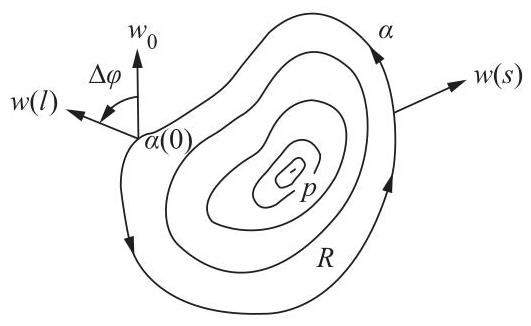
\includegraphics[max width=0.4\textwidth]{images/bo_d4b9jf3ef24c73e0334g_285_182_1074_531_326_0.jpg}
\end{center}
\hspace*{3em} 

图 4-28

现在， \({\Delta \varphi }\) 不依赖于 \({w}_{0}\) 的选择，并且从上面的表达式可知 \({\Delta \varphi }\) 也不依赖于 \(\alpha \left( 0\right)\) 的选择.通过取极限(在命题 2，第 3-3 节的意义下)

\[
\mathop{\lim }\limits_{{R \rightarrow  p}}\frac{\Delta \varphi }{A\left( R\right) } = K\left( p\right)
\]

其中 \(A\left( R\right)\) 表示区域 \(R\) 的面积，我们得到 \(K\) 的期望解释.

为了推广高斯-博内定理，我们需要进一步的拓扑预备知识.

设 \(S\) 为一个正则曲面.一个连通区域 \(R \subset  S\) 被称为正则的，如果 \(R\) 是紧致的，并且其边界 \(\partial R\) 是有限个(简单)闭合的分段正则曲线的并集，这些曲线不相交(图 4-29(a) 中的区域是正则的，但图 4-29(b) 中的不是).为方便起见，我们将紧致曲面视为一个正则区域，其边界为空.

\begin{center}
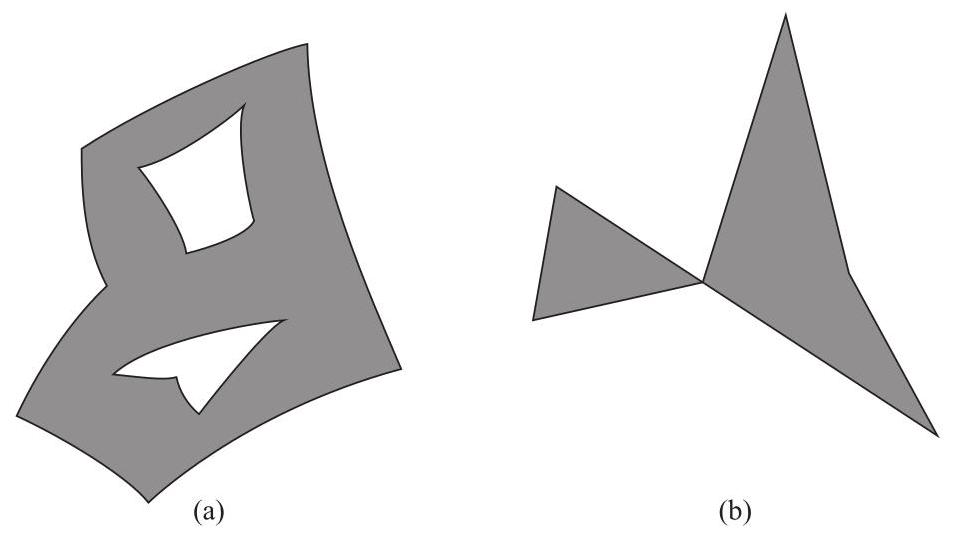
\includegraphics[max width=0.8\textwidth]{images/bo_d4b9jf3ef24c73e0334g_286_305_561_957_537_0.jpg}
\end{center}
\hspace*{3em} 

图 4-29

一个只有三个顶点且外角分别为 \({\alpha }_{i} \neq  0\) 、 \(i = l,2,3\) 的简单区域称为三角形.

正则区域 \(R \subset  S\) 的三角剖分是指一个有限的三角形 \({T}_{i}, = 1,\ldots ,n\) 的族 \(\mathfrak{J}\) ，使得

1. \(\mathop{\bigcup }\limits_{{i = 1}}^{n}{T}_{i} = R\) .

2. 如果 \({T}_{i} \cap  {T}_{j} \neq  \phi\) ，那么 \({T}_{i} \cap  {T}_{j}\) 要么是 \({T}_{i}\) 和 \({T}_{j}\) 的公共边，要么是 \({T}_{i}\) 和 \({T}_{j}\) 的公共顶点.

给定曲面 \(S\) 的正则区域 \(R \subset  S\) 的一个三角剖分 \(\mathfrak{J}\) ，我们将用 \(F\) 表示三角形(面)的数量，用 \(E\) 表示边(棱)的数量，用 \(V\) 表示三角剖分的顶点数量.数量

\[
F - E + V = \chi
\]

称为三角剖分的欧拉-庞加莱示性数.

以下命题在没有证明的情况下给出.这些事实的阐述可以在例如 L. Ahlfors 和 L. Sario 的著作 Riemann Surfaces, Princeton University Press, Princeton, N.J., 1960, Chap. 1 中找到.

命题 1. 每个正则曲面的正则区域都允许进行三角剖分.

命题 2. 设 \(S\) 为一个定向曲面， \(\left\{  {\mathbf{x}}_{\alpha }\right\}  ,\alpha  \in  \mathrm{A}\) 为与 \(S\) 的定向相容的参数化族.设 \(\mathbb{R} \subset  S\) 为 \(S\) 的一个正则区域.那么存在 \(\mathbb{R}\) 的 \(\mathfrak{J}\) 的一个三角剖分，使得每个三角形 \(\mathrm{T} \in  \mathfrak{J}\) 都包含在 \(\left\{  {\mathbf{x}}_{\alpha }\right\}\) 族中的某个坐标邻域内.此外，如果 \(\mathfrak{J}\) 中每个三角形的边界都定向为正，则相邻的三角形在公共边上确定相反的定向(图 4-30).

\begin{center}
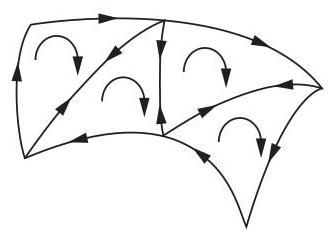
\includegraphics[max width=0.3\textwidth]{images/bo_d4b9jf3ef24c73e0334g_287_186_585_333_240_0.jpg}
\end{center}
\hspace*{3em} 

图 4-30

命题 3. 如果 \(\mathbb{R} \subset  S\) 是曲面 \(S\) 的一个正则区域，则欧拉-庞加莱示性数不依赖于 \(\mathbb{R}\) 的三角剖分.因此，将其记为 \(\chi \left( \mathbb{R}\right)\) 是方便的.

后一个命题表明欧拉-庞加莱示性数是正则区域 \(R\) 的一个拓扑不变量.为了应用高斯-博内定理，我们将提及一个重要事实，即这个不变量允许对 \({R}^{3}\) 中的紧致曲面进行拓扑分类.

直接计算表明，球体的欧拉-庞加莱示性数为 2，环面的(带有一个“把手”的球体；见图 4-31)为零，双环面的(带有两个把手的球体)为 -2，并且，一般来说， \(n\) -环面的(带 \(n\) 个把手的球体)为 \(- 2\left( {n - 1}\right)\) .

以下命题表明，此列表穷尽了 \({R}^{3}\) 中的所有紧致曲面.

命题 4. 设 \(S \subset  {\mathbb{R}}^{3}\) 是一个紧致连通曲面；则欧拉-庞加莱示性数 \(\chi \left( S\right)\) 的值之一是 \(2,0, - 2,\ldots , - 2N,\ldots\) .此外，如果 \({S}^{\prime } \subset  {\mathbb{R}}^{3}\) 是另一个紧致曲面且 \(\chi \left( S\right)  = \chi \left( {S}^{\prime }\right)\) ，则 \(S\) 同胚于 \({S}^{\prime }\) .

换句话说，每个紧致连通曲面 \(S \subset  {R}^{3}\) 都同胚于一个带有所述数量 \(g\) 的把手的球体.这个数量

\[
g = \frac{2 - \chi \left( S\right) }{2}
\]

称为 \(S\) 的亏格.

最后，设 \(R \subset  S\) 是一个定向曲面 \(S\) 的正则区域，设 \(\mathfrak{J}\) 是 \(R\) 的一个三角剖分，使得每个三角形 \({T}_{j} \in  \mathfrak{J},j = 1,\ldots ,k\) 都包含在坐标邻域 \({\mathbf{x}}_{j}\left( {U}_{j}\right)\) 中，该邻域由一组与 \(S\) 的定向兼容的参数化 \(\left\{  {\mathbf{x}}_{\alpha }\right\}  ,\alpha  \in  A\) 构成.设 \(f\) 是 \(S\) 上的一个可微函数.以下命题表明，讨论 \(f\) 在区域 \(R\) 上的积分是有意义的.

\begin{center}
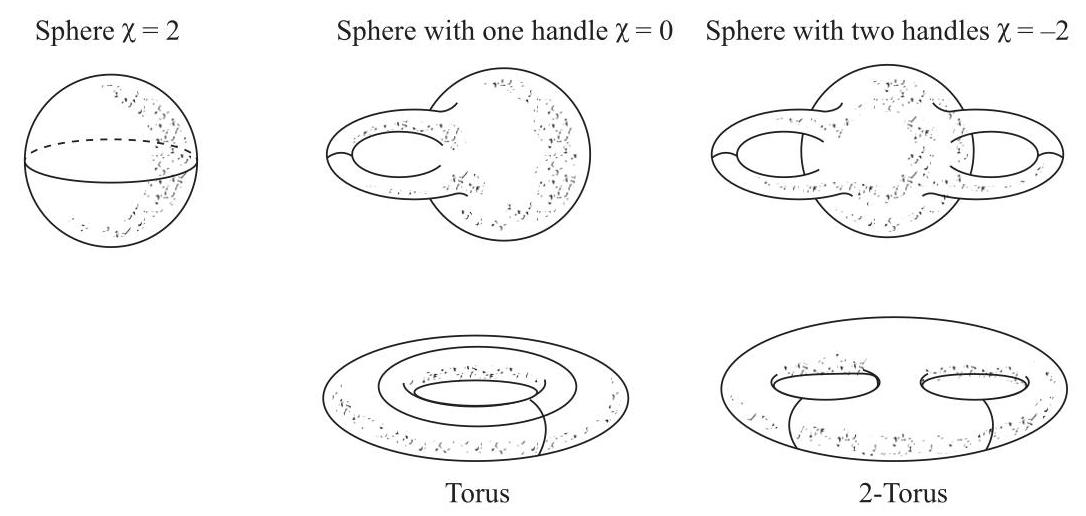
\includegraphics[max width=0.9\textwidth]{images/bo_d4b9jf3ef24c73e0334g_288_237_194_1086_516_0.jpg}
\end{center}
\hspace*{3em} 

图 4-31

命题 5. 在上述记号下，和

\[
\mathop{\sum }\limits_{{j = 1}}^{k}{\iint }_{{x}_{j}^{-1}\left( {T}_{j}\right) }f\left( {{u}_{i},{v}_{j}}\right) \sqrt{{E}_{j}{G}_{j} - {F}_{j}^{2}}d{u}_{j}d{v}_{j}
\]

不依赖于剖分 \(\mathfrak{J}\) 或 \(S\) 的参数化族 \(\left\{  {\mathbf{x}}_{\mathrm{j}}\right\}\) .

因此，这个和具有几何意义，称为 \(\mathrm{f}\) 在正则区域 \(\mathbb{R}\) 上的积分.它通常记为

\[
{\iint }_{R}{fd\sigma }
\]

现在我们可以陈述并证明

整体高斯-博内定理.设 \(\mathbb{R} \subset  S\) 是一个有向曲面上的正则区域，设 \({\mathrm{C}}_{1},\ldots ,{\mathrm{C}}_{N}\) 是构成 \(\mathbb{R}\) 的边界 \(\partial \mathbb{R}\) 的闭合、简单、分段正则曲线.假设每条 \({\mathrm{C}}_{\mathrm{i}}\) 都是正向定向的，设 \({\theta }_{1},\ldots ,{\theta }_{\mathrm{p}}\) 是曲线 \({\mathrm{C}}_{1},\ldots ,{\mathrm{C}}_{N}\) 的所有外角集合.则

\[
\mathop{\sum }\limits_{{\mathrm{i} = 1}}^{N}{\int }_{{\mathrm{c}}_{\mathrm{i}}}{\mathrm{k}}_{\mathrm{g}}\left( S\right) \mathrm{{ds}} + {\iint }_{\mathbb{R}}\mathrm{{Kd\sigma }} + \mathop{\sum }\limits_{{l = 1}}^{\mathrm{p}}{\theta }_{l} = {2\pi \chi }\left( \mathbb{R}\right) ,
\]

其中 \(S\) 表示 \({\mathrm{C}}_{\mathrm{i}}\) 的弧长，而 \({\mathrm{C}}_{\mathrm{i}}\) 上的积分表示在 \({\mathrm{C}}_{\mathrm{i}}\) 的每个正则弧上的积分之和.

证明.考虑区域 \(R\) 的一个剖分 \(\mathfrak{J}\) ，使得每个三角形 \({T}_{j}\) 都包含在与 \(S\) 的定向相容的等温参数化族的一个坐标邻域内.根据命题 2，这样的剖分存在.此外，如果 \(\mathfrak{J}\) 的每个三角形的边界都是正向定向的，那么在相邻三角形共有的边上，我们将得到相反的定向(图 4-32).

\begin{center}
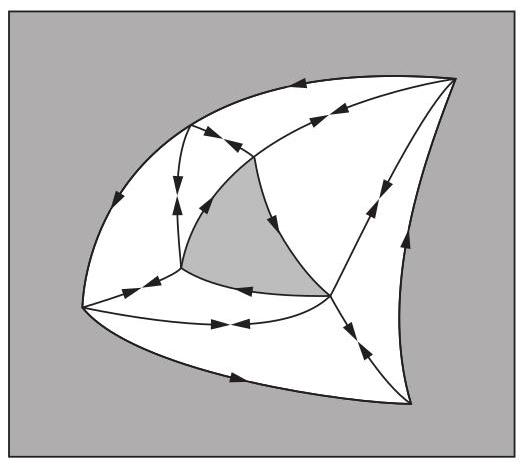
\includegraphics[max width=0.4\textwidth]{images/bo_d4b9jf3ef24c73e0334g_289_184_625_521_464_0.jpg}
\end{center}
\hspace*{3em} 

图 4-32

通过将局部高斯-博内定理应用于每个三角形并累加结果，我们得到，利用命题 5 和每个“内部”边被描述两次且方向相反的事实，

\[
\mathop{\sum }\limits_{i}{\int }_{{c}_{i}}{k}_{g}\left( s\right) {ds} + {\iint }_{R}{Kd\sigma } + \mathop{\sum }\limits_{{j,k = 1}}^{{F,3}}{\theta }_{jk} = {2\pi F},
\]

其中 \(F\) 表示 \(\mathfrak{J}\) 的三角形数量，而 \({\theta }_{j1},{\theta }_{j2},{\theta }_{j3}\) 是三角形 \({T}_{j}\) 的外角.

现在我们将引入三角形 \({T}_{j}\) 的内角，由 \({\varphi }_{jk} = \pi  - {\theta }_{jk}\) 给出.因此，

\[
\mathop{\sum }\limits_{{j,k}}{\theta }_{jk} = \mathop{\sum }\limits_{{j,k}}\pi  - \mathop{\sum }\limits_{{j,k}}{\varphi }_{jk} = {3\pi F} - \mathop{\sum }\limits_{{j,k}}{\varphi }_{jk}.
\]

我们将使用以下记号:

\[
{E}_{e} = \text{ number of external edges of }\mathfrak{J}\text{ , }
\]

\[
{E}_{i} = \text{ number of internal edges of }\mathfrak{J}\text{ , }
\]

\[
{V}_{e} = \text{ number of external vertices of }\mathfrak{J}\text{ , }
\]

\[
{V}_{i} = \text{ number of internal vertices of }\mathfrak{J}\text{ . }
\]

由于曲线 \({C}_{i}\) 是闭合的， \({E}_{e} = {V}_{e}\) .此外，通过归纳法很容易证明

\[
{3F} = 2{E}_{i} + {E}_{e}
\]

因此

\[
\mathop{\sum }\limits_{{j,k}}{\theta }_{jk} = {2\pi }{E}_{i} + \pi {E}_{e} - \mathop{\sum }\limits_{{j,k}}{\varphi }_{jk}.
\]

我们现在注意到，外部顶点可以是曲线 \({C}_{i}\) 的顶点，也可以是剖分引入的顶点.我们设 \({V}_{e} = {V}_{ec} + {V}_{et}\) ，其中 \({V}_{ec}\) 是曲线 \({C}_{i}\) 的顶点数，而 \({V}_{et}\) 是剖分的外部顶点数，这些顶点不是曲线 \({C}_{i}\) 的顶点.由于每个内部顶点的角度和为 \({2\pi }\) ，我们得到

\[
\mathop{\sum }\limits_{{j,k}}{\theta }_{jk} = {2\pi }{E}_{i} + \pi {E}_{e} - {2\pi }{V}_{i} - \pi {V}_{et} - \mathop{\sum }\limits_{l}\left( {\pi  - {\theta }_{i}}\right) .
\]

通过将 \(\pi {E}_{e}\) 加到上述表达式并从中减去，并考虑到 \({E}_{e} = {V}_{e}\) ，我们得出结论:

\[
\mathop{\sum }\limits_{{j,k}}{\theta }_{jk} = {2\pi }{E}_{i} + {2\pi }{E}_{e} - {2\pi }{V}_{i} - \pi {V}_{e} - \pi {V}_{et} - \pi {V}_{ec} + \mathop{\sum }\limits_{l}{\theta }_{i}
\]

\[
= {2\pi E} - {2\pi V} + \mathop{\sum }\limits_{i}{\theta }_{i}.
\]

通过将各部分组合起来，我们最终得到

\[
\mathop{\sum }\limits_{{i = 1}}^{n}{\int }_{{C}_{i}}{k}_{g}\left( s\right) {ds} + {\iint }_{R}{Kd\sigma } + \mathop{\sum }\limits_{{i = 1}}^{p}{\theta }_{l} = {2\pi }\left( {F - E + V}\right)
\]

\[
= {2\pi \chi }\left( R\right) \text{ . } \tag{Q.E.D.}
\]

由于简单区域的欧拉-庞加莱示性数为 1，我们得到(参见注记 1)

推论 1. 如果 R 是 S 的一个简单区域，则

\[
\mathop{\sum }\limits_{{\mathrm{i} = 0}}^{\mathrm{k}}{\int }_{{S}_{\mathrm{i}}}^{{S}_{\mathrm{i} + 1}}{\mathrm{k}}_{\mathrm{g}}\left( S\right) \mathrm{{ds}} + {\iint }_{\mathbb{R}}\mathrm{K}\mathrm{d}\sigma  + \mathop{\sum }\limits_{{\mathrm{i} = 0}}^{\mathrm{k}}{\theta }_{\mathrm{i}} = {2\pi }.
\]

考虑到一个紧致曲面可以被视为一个边界为空的区域，我们得到

推论 2. 令 \(S\) 为一个可定向的紧致曲面；则

\[
{\iint }_{S}\mathrm{{Kd}}\sigma  = {2\pi \chi }\left( S\right) .
\]

推论 2 最为引人注目.我们只需考虑一个与球面同胚的曲面的所有可能形状，就会发现它非常令人惊讶，因为在每种情况下，曲率函数都以这样的方式分布，使得“总曲率”，即 \(\iint {Kd\sigma }\) ，对于所有情况都相同.

下面我们将给出高斯-博内定理的一些应用.对于这些应用(以及本节末尾的练习)，我们方便地假设平面拓扑的一个基本事实(若尔当曲线定理)，我们将以以下形式使用它:平面中的每条闭合的分段正则曲线(因此没有自交点)是一个简单区域的边界.

1. 正曲率的紧致曲面同胚于球面.

这样的曲面的欧拉-庞加莱示性数为正，而球面是满足此条件的唯一紧致曲面 \({R}^{3}\) .

2. 令 \(S\) 为一个曲率非负或零的可定向曲面.则从一点 \(\mathrm{p} \in  S\) 出发的两条测地线 \({\gamma }_{1}\) 和 \({\gamma }_{2}\) 不能在一点 \(\mathrm{q} \in  S\) 再次相遇，使得 \({\gamma }_{1}\) 和 \({\gamma }_{2}\) 的轨迹构成 S 的一个简单区域 R 的边界.

假设相反的情况成立.根据高斯-博内定理( \(R\) 是简单的)

\[
{\iint }_{R}{Kd\sigma } + {\theta }_{1} + {\theta }_{2} = {2\pi }
\]

其中 \({\theta }_{1}\) 和 \({\theta }_{2}\) 是区域 \(R\) 的外角.由于测地线 \({\gamma }_{1}\) 和 \({\gamma }_{2}\) 不能相互相切，我们有 \({\theta }_{i} < \pi ,i = 1,2\) .另一方面， \(K \leq  0\) ，由此产生矛盾.

当 \({\theta }_{1} = {\theta }_{2} = 0\) 时，测地线 \({\gamma }_{1}\) 和 \({\gamma }_{2}\) 的轨迹构成 \(S\) 的一个简单闭合测地线(即，一条闭合的正则曲线，它是一条测地线).由此可知，在曲率为零或负的曲面上，不存在作为 \(S\) 的简单区域边界的简单闭合测地线.

3. 令 S 为一个与高斯曲率为 \(\mathrm{K} < 0\) 的圆柱面微分同胚(即，存在一个可微映射，它有一个可微的逆映射)的曲面.则 \(S\) 最多有一条简单闭合测地线.

假设 \(S\) 包含一个简单的闭合测地线 \(\mathbf{\Gamma }\) .根据应用 2，并且存在一个微分同胚 \(\varphi\) ，将 \(S\) 与一个平面 \(P\) 减去一个点 \(q \in  P,\varphi \left( \mathbf{\Gamma }\right)\) 联系起来，该点是 \(P\) 中包含 \(q\) 的一个简单区域的边界.

假设现在 \(S\) 包含另一个简单闭合测地线 \({\mathbf{\Gamma }}^{\prime }\) .我们声称 \({\mathbf{\Gamma }}^{\prime }\) 不与 \(\mathbf{\Gamma }\) 相交.否则， \(\varphi \left( \mathbf{\Gamma }\right)\) 和 \(\varphi \left( {\mathbf{\Gamma }}^{\prime }\right)\) 在两个“连续”交点 \({r}_{1}\) 和 \({r}_{2}\) 之间的弧将构成一个简单区域的边界，这与应用 2(见图 4-33)相矛盾.我们现在可以将高斯-博内定理应用于由 \(S\) 的两条简单、不相交的测地线 \(\mathbf{\Gamma }\) 和 \({\mathbf{\Gamma }}^{\prime }\) 所界定的区域 \(R\) .由于 \(\chi \left( R\right)  = 0\) ，我们得到

\[
{\iint }_{{\varphi }^{-1}\left( R\right) }{Kd\sigma } = {2\pi \chi }\left( R\right)  = 0,
\]

\begin{center}
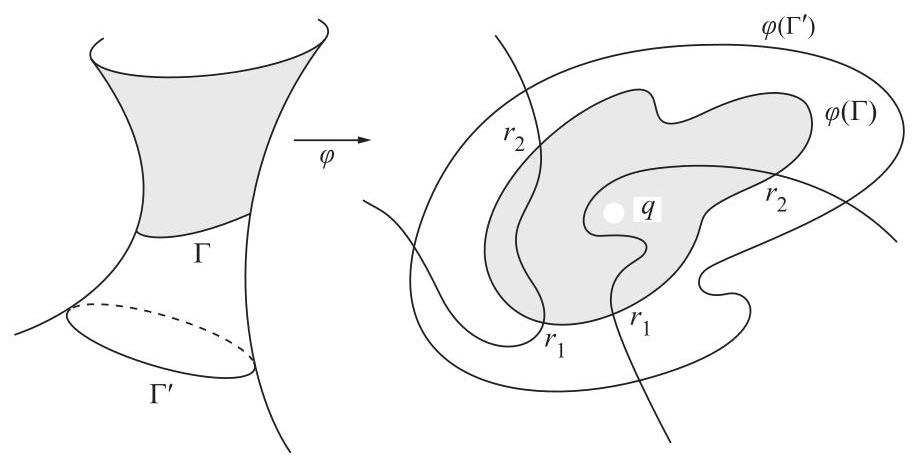
\includegraphics[max width=0.8\textwidth]{images/bo_d4b9jf3ef24c73e0334g_292_328_194_917_463_0.jpg}
\end{center}
\hspace*{3em} 

图 4-33

这与 \(K < 0\) 相矛盾.

4. 如果在具有正曲率的紧致、连通曲面 \(S\) 上存在两条简单闭合测地线 \({\mathbf{\Gamma }}_{1}\) 和 \({\mathbf{\Gamma }}_{2}\) ，则 \({\mathbf{\Gamma }}_{1}\) 和 \({\mathbf{\Gamma }}_{2}\) 相交.

根据应用 \(1,S\) 同胚于一个球面.如果 \({\mathbf{\Gamma }}_{1}\) 和 \({\mathbf{\Gamma }}_{2}\) 不相交，则由 \({\mathbf{\Gamma }}_{1}\) 和 \({\mathbf{\Gamma }}_{2}\) 组成的集合是区域 \(R\) 的边界，该区域的欧拉-庞加莱示性数为 \(\chi \left( R\right)  = 0\) .根据高斯-博内定理，

\[
{\iint }_{R}{Kd\sigma } = 0
\]

这与 \(K > 0\) 相矛盾.

5. 我们将证明雅可比的以下结果:设 \(\alpha  : \mathrm{I} \rightarrow  {\mathbb{R}}^{3}\) 为一条闭合的、正则的、参数化的曲线，其曲率非零.假设由单位球面 \({S}^{2}\) 中的法向量 \(N\left( S\right)\) (法指示曲面)描述的曲线是简单的.则 \(N\left( \mathrm{I}\right)\) 将 \({S}^{2}\) 分为两个面积相等的区域.

我们可以假设 \(\alpha\) 是由弧长参数化的.设 \(\bar{s}\) 表示曲线 \(n = n\left( s\right)\) 在 \({S}^{2}\) 上的弧长. \(n\left( s\right)\) 的测地曲率 \({\bar{k}}_{g}\) 为

\[
{\bar{k}}_{g} = \langle \ddot{n},n \land  \dot{n}\rangle ,
\]

其中点表示相对于 \(\bar{s}\) 的微分.由于

\[
\dot{n} = \frac{dn}{ds}\frac{ds}{d\bar{s}} = \left( {-{kt} - {\tau b}}\right) \frac{ds}{d\bar{s}},
\]

\[
\ddot{n} = \left( {-{kt} - {\tau b}}\right) \frac{{d}^{2}s}{d{\bar{s}}^{2}} + \left( {-{k}^{\prime }t - {\tau }^{\prime }b}\right) {\left( \frac{ds}{d\bar{s}}\right) }^{2} - \left( {{k}^{2} + {\tau }^{2}}\right) n{\left( \frac{ds}{d\bar{s}}\right) }^{2},
\]

和

\[
{\left( \frac{ds}{d\bar{s}}\right) }^{2} = \frac{1}{{k}^{2} + {\tau }^{2}},
\]

我们得到

\[
{\bar{k}}_{g} = \langle n \land  \dot{n},\ddot{n}\rangle  = \frac{ds}{d\bar{s}}\langle \left( {{kb} - {\tau t}}\right) ,\ddot{n}\rangle  = {\left( \frac{ds}{d\bar{s}}\right) }^{3}\left( {-k{\tau }^{\prime } + {k}^{\prime }\tau }\right)
\]

\[
=  - \frac{{\tau }^{\prime }k - {k}^{\prime }\tau }{{k}^{2} + {\tau }^{2}}\frac{ds}{d\bar{s}} =  - \frac{d}{ds}{\tan }^{-1}\left( \frac{\tau }{k}\right) \frac{ds}{d\bar{s}}.
\]

因此，通过将高斯-博内定理应用于 \(n\left( I\right)\) 所界定的区域 \(R\) 之一，并利用 \(K \equiv  1\) 的事实，我们得到

\[
{2\pi } = {\int }_{R}{Kd\sigma } + {\int }_{\partial R}{\bar{k}}_{g}d\bar{s} = {\int }_{R}{d\sigma } = \text{ area of }R.
\]

由于 \({S}^{2}\) 的面积为 \({4\pi }\) ，结果成立.

6. 设 \(T\) 为定向曲面 \(S\) 中的一个测地三角形(即 \(T\) 的边是测地线).假设高斯曲率 \(K\) 在 \(T\) 中不改变符号.设 \({\theta }_{1},{\theta }_{2},{\theta }_{3}\) 为 \(T\) 的外角，设 \({\varphi }_{1} = \pi  - {\theta }_{1}\) 、 \({\varphi }_{2} = \pi  - {\theta }_{2},{\varphi }_{3} = \pi  - {\theta }_{3}\) 为其内角.根据高斯-博内定理，

\[
{\iint }_{T}{Kd\sigma } + \mathop{\sum }\limits_{{i = 1}}^{3}{\theta }_{i} = {2\pi }.
\]

因此，

\[
{\iint }_{T}{Kd\sigma } = {2\pi } - \mathop{\sum }\limits_{{i = 1}}^{3}\left( {\pi  - {\varphi }_{i}}\right)  =  - \pi  + \mathop{\sum }\limits_{{i = 1}}^{3}{\varphi }_{i}.
\]

由此可知，测地三角形的内角和 \(\mathop{\sum }\limits_{{i = 1}}^{3}{\varphi }_{i}\) 为

1. 等于 \(\pi\) 如果 \(K = 0\) .

2. 大于 \(\pi\) 如果 \(K > 0\) .

3. 小于 \(\pi\) 如果 \(K < 0\) .

此外，差值 \(\mathop{\sum }\limits_{{i = 1}}^{3}{\varphi }_{i} - \pi\) ( \(T\) 的超额部分)由 \({\iint }_{T}{Kd\sigma }\) 精确给出.如果 \(K \neq  0\) 在 \(T\) 上，则这是高斯映射 \(N : S \rightarrow  {S}^{2}\) 将 \(T\) 映射到 \(N\left( T\right)\) 的图像的面积(参见第 3-3 节的公式 (12)).高斯本人陈述其定理的形式如下:测地三角形 \(\mathrm{T}\) 的超额部分等于其球面像 \(N\left( \mathrm{T}\right)\) 的面积.

上述事实与一个关于证明欧几里得第五公理(平行公理)可能性的历史争议有关，由此得出任何三角形的内角和等于 \(\pi\) .通过将测地线视为直线，可以证明常负曲率的曲面构成一个(局部)模型，其中欧几里得公理成立，但第五公理以及保证直线可以无限延长的公理除外.实际上，希尔伯特证明了在 \({R}^{3}\) 中不存在常负曲率的曲面，其测地线可以无限延长(第 3-3 节练习 6 中的伪球面有一个奇异点边缘).因此，具有常负高斯曲率的 \({R}^{3}\) 曲面不能提供一个检验第五公理独立性的模型.然而，通过使用抽象曲面的概念，可以绕过这个不便，并构建一个模型，其中除第五公理外，所有欧几里得公理都成立.因此，第五公理独立于其他公理.

在第 5-10 节和 5-11 节中，我们将证明刚刚引用的希尔伯特的结果，并描述非欧几里得几何的抽象模型.

7. 曲面上的向量场. \({}^{ \dagger  }\) 设 \(v\) 为定向曲面 \(S\) 上的可微向量场.如果 \(v\left( p\right)  = 0\) ，则称 \(p \in  S\) 是 \(v\) 的奇点.如果存在 \(S\) 中 \(p\) 的一个邻域 \(V\) ，使得 \(V\) 中除了 \(p\) 之外没有 \(v\) 的奇点，则称奇点 \(p\) 是孤立的.

对于向量场 \(v\) 的每个孤立奇异点 \(p\) ，我们将关联一个整数，即 \(v\) 的指标，定义如下.令 \(\mathbf{x} : U \rightarrow  S\) 为在 \(p = \mathbf{x}\left( {0,0}\right)\) 处与 \(S\) 的定向兼容的正交参数化，并令 \(\alpha  : \left\lbrack  {0,l}\right\rbrack   \rightarrow  S\) 为一条简单、闭合、正定向的分段正则参数化曲线，使得 \(\alpha \left( \left\lbrack  {0,l}\right\rbrack  \right)  \subset  \mathbf{x}\left( U\right)\) 是包含 \(p\) 作为其唯一奇异点的简单区域 \(R\) 的边界.令 \(v = v\left( t\right) ,t \in  \left\lbrack  {0,l}\right\rbrack\) 为 \(v\) 沿 \(\alpha\) 的限制，并令 \(\varphi  = \varphi \left( t\right)\) 为从 \({\mathbf{x}}_{u}\) 到 \(v\left( t\right)\) 的某个可微角度确定值，由第 4-4 节的引理 1 给出(该引理可以轻松扩展到分段正则曲线).由于 \(\alpha\) 是闭合的，存在一个整数 \(I\) 定义为

\[
{2\pi I} = \varphi \left( l\right)  - \varphi \left( 0\right)  = {\int }_{0}^{l}\frac{d\varphi }{dt}{dt}.
\]

\(I\) 称为 \(v\) 在 \(p\) 处的指标.



此应用需要第 3-4 节的材料.如果省略，则本节的练习 6-9 也应省略.



我们必须证明该定义独立于所做的选择，第一个选择是参数化 \(\mathbf{x}\) .令 \({w}_{0} \in  {T}_{\alpha \left( 0\right) }\left( S\right)\) ，令 \(w\left( t\right)\) 为 \({w}_{0}\) 沿 \(\alpha\) 的平行移动.令 \(\psi \left( t\right)\) 为从 \({\mathbf{x}}_{u}\) 到 \(w\left( t\right)\) 的角度的可微确定值.那么，正如我们在 \(K\) 的平行移动解释中所见(参见方程 (2))，

\[
\psi \left( l\right)  - \psi \left( 0\right)  = {\iint }_{R}{Kd\sigma }
\]

通过减去上述关系，我们得到

\[
{\iint }_{R}{Kd\sigma } - {2\pi I} = \left( {\psi  - \varphi }\right) \left( l\right)  - \left( {\psi  - \varphi }\right) \left( 0\right)  = \Delta \left( {\psi  - \varphi }\right) \tag{3}
\]

由于 \(\psi  - \varphi\) 不依赖于 \({\mathbf{x}}_{u}\) ，因此索引 \(I\) 不依赖于参数化 \(\mathbf{x}\) .

索引不依赖于 \(\alpha\) 选择的证明更为技术性(尽管相当直观)，我们将只对其进行概述.

令 \({\alpha }_{0}\) 和 \({\alpha }_{1}\) 为索引定义中的两条曲线，并证明 \(v\) 的索引对两条曲线都相同.我们首先假设 \({\alpha }_{0}\) 和 \({\alpha }_{1}\) 的轨迹不相交.那么存在一个同胚，将 \({\alpha }_{0}\) 和 \({\alpha }_{1}\) 轨迹所围成的区域映射到平面上由两条同心圆 \({C}_{0}\) 和 \({C}_{1}\) (一个环形区域)围成的区域.由于我们可以得到一个 \({C}_{t}\) 的同心圆族，它连续依赖于 \(t\) 并将 \({C}_{0}\) 变形为 \({C}_{1}\) ，我们得到一个 \({\alpha }_{t}\) 的曲线族，它连续依赖于 \(t\) 并将 \({\alpha }_{0}\) 变形为 \({\alpha }_{1}\) (图 4-34).令 \({I}_{t}\) 为使用曲线 \({\alpha }_{t}\) 计算的 \(v\) 的索引.现在，由于索引是一个积分， \({I}_{t}\) 连续依赖于 \(t,t \in  \left\lbrack  {0,1}\right\rbrack\) .由于 \({I}_{t}\) 是一个整数，在变形过程中它是恒定的，因此得到 \({I}_{0} = {I}_{1}\) ，正如我们所希望的.如果 \({\alpha }_{0}\) 和 \({\alpha }_{1}\) 的轨迹相交，我们选择一条足够小的曲线，使其轨迹与 \({\alpha }_{0}\) 和 \({\alpha }_{1}\) 都不相交，然后应用前面的结果.

应该注意的是，即使 \(p\) 不是 \(v\) 的奇异点，索引的定义仍然适用.然而，结果是索引为零.

\begin{center}
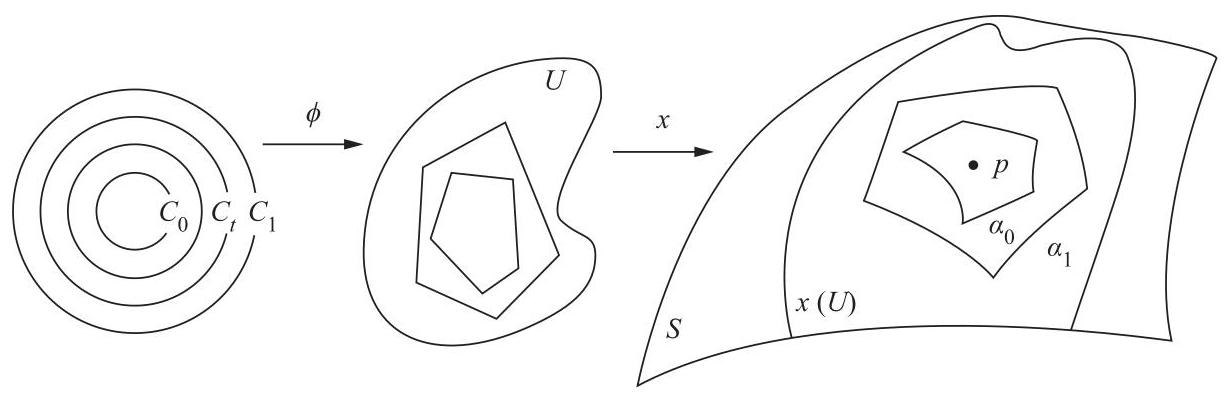
\includegraphics[max width=1.0\textwidth]{images/bo_d4b9jf3ef24c73e0334g_295_180_1646_1231_397_0.jpg}
\end{center}
\hspace*{3em} 

图 4-34

这是因为，由于 \(I\) 不依赖于 \({\mathbf{x}}_{u}\) ，我们可以选择 \({\mathbf{x}}_{u}\) 为 \(v\) 本身；因此， \(\varphi \left( t\right)  \equiv  0\) .

在图 4-35 中，我们展示了一些在 \({xy}\) 平面上具有 \(\left( {0,0}\right)\) 作为奇异点的向量场的索引示例.图中出现的曲线是向量场的轨迹.

\begin{center}
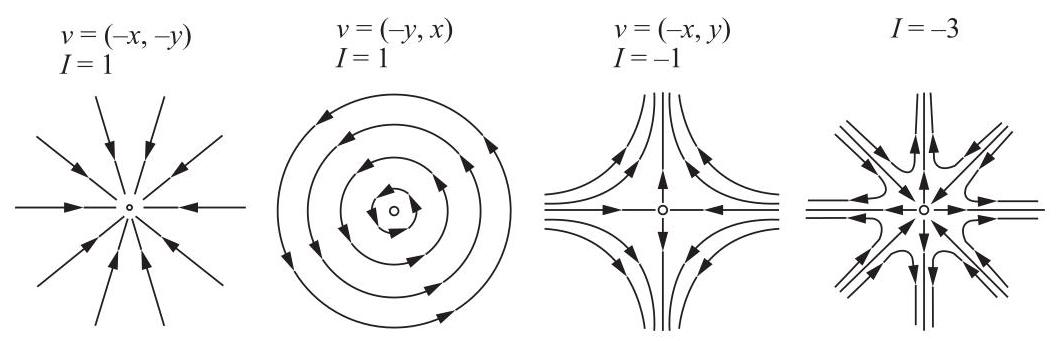
\includegraphics[max width=0.9\textwidth]{images/bo_d4b9jf3ef24c73e0334g_296_253_495_1056_341_0.jpg}
\end{center}
\hspace*{3em} 

图 4-35

现在，设 \(S \subset  {R}^{3}\) 为一个定向的紧致曲面， \(v\) 为一个只有孤立奇点的可微向量场.我们注意到它们的数量是有限的.否则，根据紧致性(参见第 2-7 节，性质 1)，它们会有一个极限点，这是一个非孤立的奇点.设 \(\left\{  {\mathbf{x}}_{\alpha }\right\}\) 为一组与 \(S\) 的定向相容的正交参数化.设 \(\mathfrak{J}\) 为 \(S\) 的一个三角剖分，使得

1. 每个三角形 \(T \in  \mathfrak{J}\) 都包含在 \(\left\{  {\mathbf{x}}_{\alpha }\right\}\) 的某个坐标邻域内.

2. 每个 \(T \in  \mathfrak{J}\) 最多包含一个奇点.

3. 每个 \(T \in  \mathfrak{J}\) 的边界不包含奇点且是正定向的.

如果我们对每个三角形 \(T \in  \mathfrak{J}\) 应用公式 (3)，将结果相加，并考虑到每个 \(T \in  \mathfrak{J}\) 的边出现两次且方向相反，我们得到

\[
{\iint }_{s}{Kd\sigma } - {2\pi }\mathop{\sum }\limits_{{i = 1}}^{k}{I}_{i} = 0,
\]

其中 \({I}_{i}\) 是奇点 \({p}_{i},i = 1,\ldots ,k\) 的指数.结合高斯-博内定理(参见推论 2)，我们最终得到

\[
\sum {I}_{i} = \frac{1}{2\pi }{\iint }_{S}{Kd\sigma } = \chi \left( S\right) .
\]

因此，我们证明了以下内容:

庞加莱定理.具有孤立奇点的可微向量场 \(\mathrm{v}\) 在紧致曲面 \(S\) 上的指数之和等于 \(S\) 的欧拉-庞加莱示性数.

这是一个了不起的结果.它意味着 \(\sum {I}_{i}\) 不依赖于 \(v\) ，而只依赖于 \(S\) 的拓扑.例如，在任何同胚于球面的曲面上，所有具有孤立奇点的向量场的指数之和必须等于 2.特别地，任何这样的曲面都不可能有一个没有奇点的可微向量场.

\exerciseline

1. 设 \(S \subset  {R}^{3}\) 为一个正则、紧致、连通、可定向曲面，它不同胚于球面.证明 \(S\) 上存在高斯曲率为正、负和零的点.

2. 设 \(T\) 为一个旋转环面.描述 \(T\) 的高斯映射的像，并证明(不使用高斯-博内定理)

\[
{\iint }_{T}{Kd\sigma } = 0.
\]

计算 \(T\) 的欧拉-庞加莱示性数，并用高斯-博内定理检验上述结果.

3. 设 \(S \subset  {R}^{3}\) 为一个正则紧致曲面，其 \(K > 0\) .设 \(\Gamma  \subset  S\) 为 \(S\) 中的一个简单闭合测地线，设 \(A\) 和 \(B\) 为 \(S\) 中以 \(\mathbf{\Gamma }\) 为公共边界的区域.设 \(N : S \rightarrow  {S}^{2}\) 为 \(S\) 的高斯映射.证明 \(N\left( A\right)\) 和 \(N\left( B\right)\) 的面积相等.

4. 计算的欧拉-庞加莱示性数

a. 一个椭球体.

*.b. 表面 \(S = \left\{  {\left( {x,y,z}\right)  \in  {R}^{3};{x}^{2} + {y}^{10} + {z}^{6} = 1}\right\}\) .

5. 令 \(C\) 为定向单位球面 \({S}^{2}\) 上的余纬平行圈 \(\varphi\) ，令 \({w}_{0}\) 为在点 \(p \in  C\) 处切于 \(C\) 的单位向量(参见示例 1，第 4-4 节).将 \({w}_{0}\) 沿 \(C\) 进行平行移动，并证明经过一整圈后，其位置与初始位置 \({w}_{0}\) 之间的夹角为 \({\Delta \varphi } = {2\pi }\left( {1 - \cos \varphi }\right)\) .验证

\[
\mathop{\lim }\limits_{{R \rightarrow  p}}\frac{\Delta \varphi }{A} = 1 = \text{ curvature of }{S}^{2},
\]

其中 \(A\) 是 \({S}^{2}\) 中由 \(C\) 围成的区域 \(R\) 的面积.

6. 证明 \(\left( {0,0}\right)\) 是一个孤立奇点，并计算平面上以下向量场在 \(\left( {0,0}\right)\) 处的指标:

*a. \(v = \left( {x,y}\right)\) .

b. \(v = \left( {-x,y}\right)\) .

c. \(v = \left( {x, - y}\right)\) .

*d. \(v = \left( {{x}^{2} - {y}^{2}, - {2xy}}\right)\) .

e. \(v = \left( {{x}^{3} - {3x}{y}^{2},{y}^{3} - 3{x}^{2}y}\right)\) .

7. 奇点的指标会为零吗？如果会，请举例说明.

8. 证明一个可定向的紧致曲面 \(S \subset  {R}^{3}\) 存在一个无奇点的可微向量场，当且仅当 \(S\) 与环面同胚.

9. 令 \(C\) 为球面 \({S}^{2}\) 上的一条正则闭合简单曲线.令 \(v\) 为 \({S}^{2}\) 上一个具有孤立奇点的可微向量场，使得 \(v\) 的轨迹从不与 \(C\) 相切.证明 \(C\) 确定的两个区域中的每一个都包含至少一个 \(v\) 的奇点.

\section*{4-6. 指数映射.测地极坐标}

在本节中，我们将介绍一些特殊的坐标系，并着眼于它们的几何应用.引入此类坐标的自然方式是通过指数映射，我们现在将对此进行描述.

正如我们在第 4-4 节命题 5 中所学到的，给定一个正则曲面 \(S\) 上的点 \(p\) 和一个非零向量 \(v \in  {T}_{p}\left( S\right)\) ，存在一个唯一的参数化测地线 \(\gamma  : \left( {-\epsilon ,\epsilon }\right)  \rightarrow  S\) ，其初始点为 \(\gamma \left( 0\right)  = p\) 且初始方向为 \({\gamma }^{\prime }\left( 0\right)  = v\) .为了表示该测地线对向量 \(v\) 的依赖性，我们方便地将其记为 \(\gamma \left( {t,v}\right)  = \gamma\) .

引理 1. 如果测地线 \(\gamma \left( {\mathrm{t},\mathrm{v}}\right)\) 对 \(\mathrm{t} \in  \left( {-\epsilon ,\epsilon }\right)\) 定义，则测地线 \(\gamma \left( {\mathrm{t},\lambda \mathrm{v}}\right) ,\lambda  \in  \mathbb{R},\lambda  > 0\) 对 \(\mathrm{t} \in  \left( {-\epsilon /\lambda ,\epsilon /\lambda }\right)\) 定义，并且 \(\gamma \left( {\mathrm{t},\lambda \mathrm{v}}\right)  = \gamma \left( {\lambda \mathrm{t},\mathrm{v}}\right) .\)

证明.令 \(\alpha  : \left( {-\epsilon /\lambda ,\epsilon /\lambda }\right)  \rightarrow  S\) 为由 \(\alpha \left( t\right)  = \gamma \left( {\lambda t}\right)\) 定义的参数化曲线.则 \(\alpha \left( 0\right)  = \gamma \left( 0\right) ,{\alpha }^{\prime }\left( 0\right)  = \lambda {\gamma }^{\prime }\left( 0\right)\) ，并且，由于 \(D\) 的线性(参见第 4-4 节方程 (1))，

\[
{D}_{{\alpha }^{\prime }\left( t\right) }{\alpha }^{\prime }\left( t\right)  = {\lambda }^{2}{D}_{{\gamma }^{\prime }\left( t\right) }{\gamma }^{\prime }\left( t\right)  = 0.
\]

因此， \(\alpha\) 是一个具有初始条件 \(\gamma \left( 0\right) ,\lambda {\gamma }^{\prime }\left( 0\right)\) 的测地线，并且根据唯一性

\[
\alpha \left( t\right)  = \gamma \left( {t,{\lambda v}}\right)  = \gamma \left( {{\lambda t},v}\right) \tag{Q.E.D.}
\]

直观地说，引理 1 意味着，由于测地线的速度是恒定的，我们可以通过适当调整速度，在规定时间内沿着其轨迹前进.

我们现在引入以下记法.如果 \(v \in  {T}_{p}\left( S\right) ,v \neq  0\) 使得 \(\gamma \left( {\left| v\right| ,v/\left| v\right| }\right)  = \gamma \left( {1,v}\right)\) 有定义，我们则设定

\[
{\exp }_{p}\left( v\right)  = \gamma \left( {1,v}\right) \;\text{ and }\;{\exp }_{p}\left( 0\right)  = p.
\]

在几何上，该构造对应于沿着通过 \(p\) 的测地线，在 \(v\) 的方向上(如果可能)截取长度等于 \(\left| v\right|\) 的线段；由此得到的 \(S\) 的点记为 \({\exp }_{p}\left( v\right)\) (图 4-36).

\begin{center}
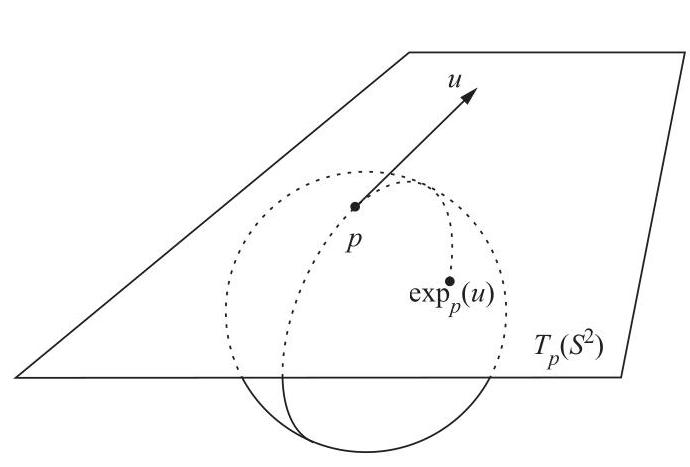
\includegraphics[max width=0.6\textwidth]{images/bo_d4b9jf3ef24c73e0334g_299_179_799_690_467_0.jpg}
\end{center}
\hspace*{3em} 

图 4-36

\begin{center}
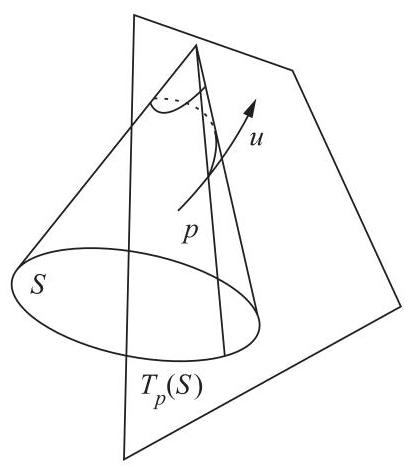
\includegraphics[max width=0.3\textwidth]{images/bo_d4b9jf3ef24c73e0334g_299_939_791_412_467_0.jpg}
\end{center}
\hspace*{3em} 

图 4-37

例如，对于单位球面 \({S}^{2}\) 上的每个 \(v \in  {T}_{p}\left( {S}^{2}\right)\) ， \({\exp }_{p}\left( v\right)\) 都有定义.半径为 \(\pi ,{3\pi },\ldots ,\left( {{2n} + 1}\right) \pi\) 的圆上的点被映射到点 \(q\) ，即 \(p\) 的对径点.半径为 \({2\pi },{4\pi },\ldots ,{2n\pi }\) 的圆上的点被映射回 \(p\) .

另一方面，在由单叶锥体(除去顶点)构成的正则曲面 \(C\) 上，对于指向连接 \(p\) 与顶点的子午线的向量 \(v \in  {T}_{p}\left( C\right)\) ，当 \(\left| v\right|  \geq  d\) 且 \(d\) 是 \(p\) 到顶点的距离时， \({\exp }_{p}\left( v\right)\) 没有定义 (图 4-37).

如果在球面的例子中，我们从 \({S}^{2}\) 中移除 \(p\) 的对径点，那么 \({\exp }_{p}\left( v\right)\) 只在以原点为中心、半径为 \(\pi\) 的 \({T}_{p}\left( {S}^{2}\right)\) 圆盘的内部有定义.

关键在于 \({\exp }_{p}\) 在 \({T}_{p}\left( S\right)\) 的原点附近的某个邻域内总是定义且可微的.

命题 1. 给定 \(\mathrm{p} \in  S\) ，存在一个 \(\epsilon  > 0\) ，使得 \({\exp }_{\mathrm{p}}\) 在以原点为中心、半径为 \(\epsilon\) 的 \({\mathrm{T}}_{\mathrm{p}}\left( S\right)\) 圆盘的内部 \({\mathrm{B}}_{\epsilon }\) 有定义且可微.

证明.显然，对于 \({T}_{p}\left( S\right)\) 的每个方向，根据引理 1，可以选择足够小的 \(v\) ，使得 \(\gamma \left( {t,v}\right)\) 的定义区间包含 1，因此 \(\gamma \left( {1,v}\right)  = {\exp }_{p}\left( v\right)\) 有定义.为了证明这种缩减可以统一地在所有方向上进行，我们需要测地线依赖于其初始条件的定理(见第 4-7 节)，其形式如下:给定 \(\mathrm{p} \in  S\) ，存在数 \({\epsilon }_{1} > 0,{\epsilon }_{2} > 0\) 和一个可微映射

\[
\gamma  : \left( {-{\epsilon }_{2},{\epsilon }_{2}}\right)  \times  {B}_{{\epsilon }_{1}} \rightarrow  S
\]

使得对于 \(\mathrm{v} \in  {\mathrm{B}}_{{\epsilon }_{1}},\mathrm{v} \neq  0,\mathrm{t} \in  \left( {-{\epsilon }_{2},{\epsilon }_{2}}\right)\) ，曲线 \(\gamma \left( {\mathrm{t},\mathrm{v}}\right)\) 是 \(S\) 的测地线，具有 \(\gamma \left( {0,\mathrm{v}}\right)  = p,{\gamma }^{\prime }\left( {0,\mathrm{v}}\right)  = \mathrm{v}\) ，并且对于 \(\mathrm{v} = 0,\gamma \left( {\mathrm{t},0}\right)  = \mathrm{p}\) .

从这个陈述和引理 1，我们的断言成立.事实上，由于 \(\gamma \left( {t,v}\right)\) 对 \(\left| t\right|  < {\epsilon }_{2},\left| v\right|  < {\epsilon }_{1}\) 定义，通过在引理 1 中设置 \(\lambda  = {\epsilon }_{2}/2\) ，我们得到 \(\gamma \left( {t,\left( {{\epsilon }_{2}/2}\right) v}\right)\) 对 \(\left| t\right|  < 2,\left| v\right|  < {\epsilon }_{1}\) 定义.因此，通过取一个以原点为中心、半径为 \(\epsilon  < {\epsilon }_{1}{\epsilon }_{2}/2\) 的圆盘 \({B}_{\epsilon } \subset  {T}_{p}\left( S\right)\) ，我们得到 \(\gamma \left( {1,w}\right)  = {\exp }_{p}w,w \in  {B}_{\epsilon }\) 已定义. \({\exp }_{p}\) 在 \({B}_{\epsilon }\) 中的可微性源于 \(\gamma\) 的可微性.Q.E.D.

这个结果的一个重要补充是:

命题 2. \({\exp }_{p} : {\mathrm{B}}_{\epsilon } \subset  {\mathrm{T}}_{\mathrm{p}}\left( S\right)  \rightarrow  S\) 是 \({\mathrm{T}}_{\mathrm{p}}\left( S\right)\) 原点 \(\mathrm{U} \subset  \mathrm{B}\) 的邻域中的一个微分同胚.

证明.我们将证明微分 \(d\left( {\exp }_{p}\right)\) 在 \(0 \in \; {T}_{p}\left( S\right)\) 处是非奇异的.为此，我们将 \({T}_{p}\left( S\right)\) 在 0 处的切向量空间与 \({T}_{p}\left( S\right)\) 本身等同起来.考虑曲线 \(\alpha \left( t\right)  = {tv},v \in  {T}_{p}\left( S\right)\) .显然 \(\alpha \left( 0\right)  = 0\) 和 \({\alpha }^{\prime }\left( 0\right)  = v\) .曲线 \(\left( {{\exp }_{p} \circ  \alpha }\right) \left( t\right)  = {\exp }_{p}\left( {tv}\right)\) 在 \(t = 0\) 处具有切向量

\[
{\left. \frac{d}{dt}\left( {\exp }_{p}\left( tv\right) \right) \right| }_{t = 0} = {\left. \frac{d}{dt}\left( \gamma \left( t,v\right) \right) \right| }_{t = 0} = v.
\]

由此得出

\[
{\left( d{\exp }_{p}\right) }_{0} = v
\]

这表明 \(d{\exp }_{p}\) 在 0 处是非奇异的.通过应用反函数定理(参见第 2-4 节的命题 3)，我们完成了命题的证明.Q.E.D.

为了方便起见，我们将 \(V \subset  S\) 称为 \(p \in  S\) 的正常邻域，如果 \(V\) 是 \({T}_{p}\left( S\right)\) 原点的一个邻域 \(U\) 的像 \(V = {\exp }_{p}\left( U\right)\) ，并且在 \({\exp }_{p}\) 上是微分同胚的.

由于 \(p \in  S\) 处的指数映射在 \(U\) 上是微分同胚的，因此可以用来在 \(V\) 中引入坐标.在这样引入的坐标系中，最常用的是

\begin{center}
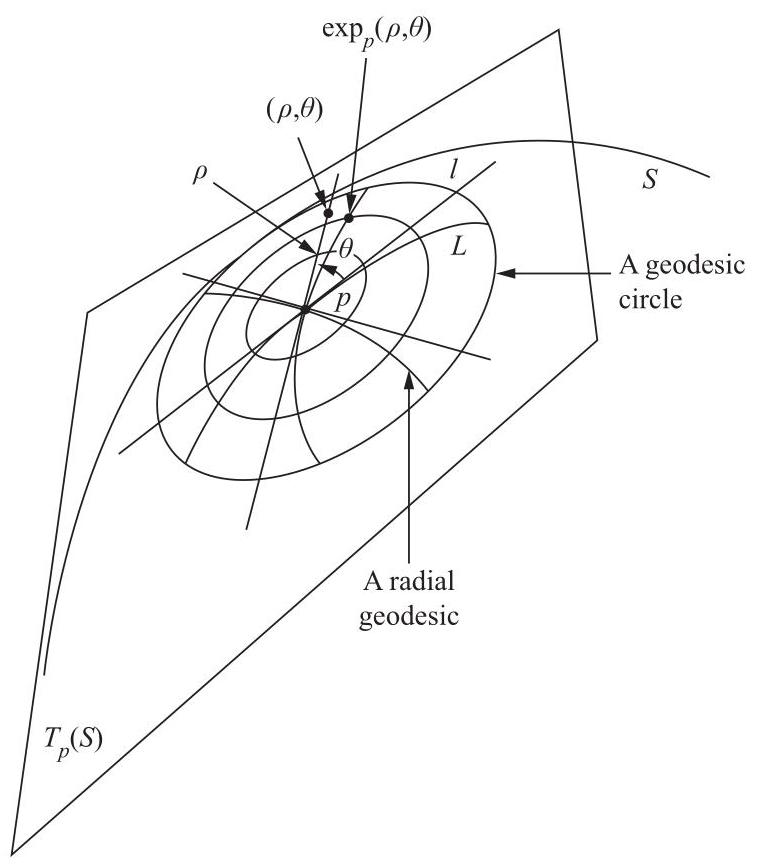
\includegraphics[max width=0.6\textwidth]{images/bo_d4b9jf3ef24c73e0334g_301_389_191_757_867_0.jpg}
\end{center}
\hspace*{3em} 

图 4-38. 极坐标.

1. 与切平面 \({T}_{p}\left( S\right)\) 中的直角坐标系相对应的法坐标.

2. 与切平面 \({T}_{p}\left( S\right)\) 中的极坐标相对应的测地极坐标 (图 4-38).

我们首先研究法坐标，它通过在平面 \({T}_{p}\left( S\right) ,p \in  S\) 中选择两个正交单位向量 \({e}_{1}\) 和 \({e}_{2}\) 来获得.由于 \({\exp }_{p} : U \rightarrow  V \subset  S\) 是一个微分同胚，它满足 \(p\) 中的参数化条件.如果 \(q \in  V\) ，则 \(q = {\exp }_{p}\left( w\right)\) ，其中 \(w = u{e}_{1} + v{e}_{2} \in  U\) ，并且我们称 \(q\) 具有坐标 \(\left( {u,v}\right)\) .显然，由此获得的法坐标取决于 \({e}_{1},{e}_{2}\) 的选择.

在以 \(p\) 为中心的法坐标系中，通过 \(p\) 的测地线是 \({\exp }_{p}\) 到通过 \({T}_{p}\left( S\right)\) 原点的直线 \(u = {at},v = {bt}\) 的像.还要注意，在 \(p\) 处，该坐标系中第一基本形式的系数由 \(E\left( p\right)  = G\left( p\right)  = 1,F\left( p\right)  = 0\) 给出.

现在我们来处理测地极坐标.在平面 \({T}_{p}\left( S\right) ,p \in  S\) 中选择一个极坐标系 \(\left( {\rho ,\theta }\right)\) ，其中 \(\rho\) 是极径， \(\theta ,0 < \theta  < {2\pi }\) 是极角，其极点是 \({T}_{p}\left( S\right)\) 的原点 0.请注意，平面中的极坐标未在闭半直线 \(l\) 上定义，该半直线对应于 \(\theta  = 0\) .设 \({\exp }_{p}\left( l\right)  = L\) .

由于 \({\exp }_{p} : U - l \rightarrow  V - L\) 仍然是一个微分同胚，我们可以用坐标 \(\left( {\rho ,\theta }\right)\) 来参数化 \(V - L\) 的点，这些坐标称为测地极坐标.

我们将使用以下术语. \({\exp }_{p} : U \rightarrow  V\) 到以 0 为中心的 \(U\) 中的圆的像将被称为 \(V\) 的测地圆， \({\exp }_{p}\) 到通过 0 的直线的像将被称为 \(V\) 的径向测地线.在 \(V - L\) 中，它们分别是曲线 \(\rho  =\) = 常数和 \(\theta  =\) = 常数.

现在我们将确定测地极坐标系中第一基本形式的系数.

命题 3. 设 \(x : \mathrm{U} - 1 \rightarrow  \mathrm{V} - \mathrm{L}\) 为一个测地极坐标系 \(\left( {\rho ,\theta }\right)\) .则第一基本形式的系数 \(\mathrm{E} = \mathrm{E}\left( {\rho ,\theta }\right) ,\mathrm{F} = \mathrm{F}\left( {\rho ,\theta }\right)\) 和 \(\mathrm{G} = \; \mathrm{G}\left( {\rho ,\theta }\right)\) 满足条件

\[
\mathrm{E} = 1,\;\mathrm{\;F} = 0,\;\mathop{\lim }\limits_{{\rho  \rightarrow  0}}\mathrm{G} = 0,\;\mathop{\lim }\limits_{{\rho  \rightarrow  0}}{\left( \sqrt{\mathrm{G}}\right) }_{\rho } = 1.
\]

证明.根据指数映射的定义， \(\rho\) 测量沿曲线 \(\theta  =\) = 常数的弧长.由此可直接得出 \(E = 1\) .

为了证明 \(F = 0\) ，我们首先证明 \({F}_{\rho } = 0\) .由于 \(\left\langle  {\frac{\partial \mathbf{x}}{\partial \rho },\frac{\partial \mathbf{x}}{\partial \theta }}\right\rangle   = F\) ，我们得到

\[
{F}_{\rho } = \left\langle  {\frac{{\partial }^{2}\mathbf{x}}{\partial {\rho }^{2}},\frac{\partial \mathbf{x}}{\partial \theta }}\right\rangle   + \left\langle  {\frac{\partial \mathbf{x}}{\partial \rho },\frac{{\partial }^{2}\mathbf{x}}{\partial \theta \partial \rho }}\right\rangle  .
\]

由于 \(\theta  =\) 是测地线，我们有

\[
{F}_{\rho } = \left\langle  {\frac{\partial \mathbf{x}}{\partial \rho },\frac{\partial }{\partial \theta }\left( \frac{\partial \mathbf{x}}{\partial \rho }\right) }\right\rangle
\]

\[
= \frac{1}{2}\frac{\partial }{\partial \theta } + \left\langle  {\frac{\partial \mathbf{x}}{\partial \rho },\frac{\partial \mathbf{x}}{\partial \rho }}\right\rangle   = 0,
\]

正如我们所声称的.因此 \(F\left( {\rho ,\theta }\right)\) 不依赖于 \(\rho\) .

对于每个 \(q \in  V\) ，我们将用 \(\alpha \left( \sigma \right)\) 表示通过 \(q\) 的测地圆，其中 \(\sigma  \in  \left\lbrack  {0,{2\pi }}\right\rbrack\) (如果 \(q = p,\alpha \left( \sigma \right)\) 是常数曲线 \(\alpha \left( \sigma \right)  = p\) ).我们将用 \(\gamma \left( s\right)\) 表示通过 \(q\) 的径向测地线，其中 \(s\) 是 \(\gamma\) 的弧长.用这个记号，我们可以写出

\[
F\left( {\rho ,\theta }\right)  = \left\langle  {\frac{d\alpha }{d\sigma },\frac{d\gamma }{ds}}\right\rangle  .
\]

系数 \(F\left( {\rho ,\theta }\right)\) 在 \(p\) 处未定义.然而，如果我们固定径向测地线 \(\theta  =\) 为常数，则上述方程的第二项对于该测地线的每一点都已定义.由于在 \(p,\alpha \left( \sigma \right)  = p\) ，即 \({d\alpha }/{d\sigma } = 0\) ，我们得到

\[
\mathop{\lim }\limits_{{\rho  \rightarrow  0}}F\left( {\rho ,\theta }\right)  = \mathop{\lim }\limits_{{\rho  \rightarrow  0}}\left\langle  {\frac{d\alpha }{d\sigma },\frac{d\gamma }{ds}}\right\rangle   = 0.
\]

连同 \(F\) 不依赖于 \(\rho\) 这一事实，这表明 \(F = 0\) .

为了证明命题的最后一个论断，我们在 \(p\) 中选择一个法坐标系 \(\left( {\bar{u},\bar{v}}\right)\) ，使得坐标变换由下式给出

\[
\bar{u} = \rho \cos \theta ,\;\bar{v} = \rho \sin \theta ,\;\rho  \neq  0,\;0 < \theta  < {2\pi }.
\]

回想一下

\[
\sqrt{{EG} - {F}^{2}} = \sqrt{\bar{E}\bar{G} - {F}^{2}}\frac{\partial \left( {\bar{u},\bar{v}}\right) }{\partial \left( {\rho ,\theta }\right) },
\]

其中 \(\partial \left( {\bar{u},\bar{v}}\right) /\partial \left( {\rho ,\theta }\right)\) 是坐标变换的雅可比行列式， \(\bar{E},\bar{F},\bar{G}\) 是法坐标系 \(\left( {\bar{u},\bar{v}}\right)\) 下的第一基本形式的系数，我们有

\[
\sqrt{G} = \rho \sqrt{\bar{E}\bar{G} - {\bar{F}}^{2}},\;\rho  \neq  0. \tag{1}
\]

由于在 \(p,\bar{E} = \bar{G} = 1,\bar{F} = 0\) (法坐标系定义在 \(p\) 处)，我们得出

\[
\mathop{\lim }\limits_{{\rho  \rightarrow  0}}\sqrt{G} = 0,\;\mathop{\lim }\limits_{{\rho  \rightarrow  0}}{\left( \sqrt{G}\right) }_{\rho } = 1,
\]

这就完成了命题的证明.Q.E.D.

注1. \(F = 0\) 这一事实的几何意义是，在法邻域中，测地圆族与径向测地线族正交.这一事实被称为高斯引理.

现在我们将给出测地极坐标的一些几何应用.

首先，我们将研究高斯曲率为常数的曲面.由于在极坐标系 \(E = 1\) 和 \(F = 0\) 中，高斯曲率 \(K\) 可以写成

\[
K =  - \frac{{\left( \sqrt{G}\right) }_{\rho \rho }}{\sqrt{G}}.
\]

如果我们要使曲面(在所讨论的坐标邻域中)具有曲率 \(K\left( {\rho ,\theta }\right)\) ，则该表达式可以视为 \(\sqrt{G}\left( {\rho ,\theta }\right)\) 应满足的微分方程.如果 \(K\) 是常数，则上述表达式，或等价地，

\[
{\left( \sqrt{G}\right) }_{\rho \rho } + K\sqrt{G} = 0, \tag{2}
\]

是一个具有常系数的二阶线性微分方程.我们将证明

定理 (Minding).任何两个具有相同常数高斯曲率的正则曲面在局部上都是等距的.更精确地说，设 \({S}_{1},{\mathrm{\;S}}_{2}\) 为具有相同常数曲率 K 的两个正则曲面.选择点 \({\mathrm{p}}_{1} \in  {S}_{1},{\mathrm{p}}_{2} \in  {S}_{2}\) 和标准正交基 \(\left\{  {{\mathrm{e}}_{1},{\mathrm{e}}_{2}}\right\}   \subset  {\mathrm{T}}_{{\mathrm{p}}_{1}}\left( {\mathrm{\;S}}_{1}\right) ,\left\{  {{\mathrm{f}}_{1},{\mathrm{f}}_{2}}\right\}   \subset  {\mathrm{T}}_{{\mathrm{p}}_{2}}\left( {\mathrm{\;S}}_{2}\right)\) .则存在邻域 \({\mathrm{V}}_{1}\) ， \({\mathrm{p}}_{1},{\mathrm{\;V}}_{2}\) 和 \({\mathrm{p}}_{2}\) ，以及一个等距映射 \(\psi  : {\mathrm{V}}_{1} \rightarrow  {\mathrm{V}}_{2}\) ，使得 \(\mathrm{d}\psi \left( {\mathrm{e}}_{1}\right)  = {\mathrm{f}}_{1},\mathrm{\;d}\psi \left( {\mathrm{e}}_{2}\right)  = {\mathrm{f}}_{2}\) .

证明.我们首先考虑方程 (2)，并分别研究情况 (1) \(K = 0,\left( 2\right) K > 0\) 和 \(\left( 3\right) K < 0\) .

1. 如果 \(K = 0,{\left( \sqrt{G}\right) }_{\rho \rho } = 0\) .因此， \({\left( \sqrt{G}\right) }_{\rho } = g\left( \theta \right)\) ，其中 \(g\left( \theta \right)\) 是 \(\theta\) 的函数.由于

\[
\mathop{\lim }\limits_{{\rho  \rightarrow  0}}{\left( \sqrt{G}\right) }_{\rho } = 1
\]

我们得出 \({\left( \sqrt{G}\right) }_{\rho } \equiv  1\) .因此， \(\sqrt{G} = \rho  + f\left( \theta \right)\) ，其中 \(f\left( \theta \right)\) 是 \(\theta\) 的函数.由于

\[
f\left( \theta \right)  = \mathop{\lim }\limits_{{\rho  \rightarrow  0}}\sqrt{G} = 0,
\]

在此情况下，我们最终得到

\[
E = 1,\;F = 0,\;G\left( {\rho ,\theta }\right)  = {\rho }^{2}.
\]

2. 如果 \(K > 0\) ，方程 (2) 的通解由下式给出

\[
\sqrt{G} = A\left( \theta \right) \cos \left( {\sqrt{K}\rho }\right)  + B\left( \theta \right) \sin \left( {\sqrt{K}\rho }\right) ,
\]

其中 \(A\left( \theta \right)\) 和 \(B\left( \theta \right)\) 是 \(\theta\) 的函数.通过微分可以轻松验证该表达式是方程 (2) 的解.

由于 \(\mathop{\lim }\limits_{{\rho  \rightarrow  0}}\sqrt{G} = 0\) ，我们得到 \(A\left( \theta \right)  = 0\) .因此，

\[
{\left( \sqrt{G}\right) }_{\rho } = B\left( \theta \right) \sqrt{K}\cos \left( {\sqrt{K}\rho }\right) ,
\]

并且由于 \(\mathop{\lim }\limits_{{\rho  \rightarrow  0}}{\left( \sqrt{G}\right) }_{\rho } = 1\) ，我们得出

\[
B\left( \theta \right)  = \frac{1}{\sqrt{K}}.
\]

因此，在此情况下，

\[
E = 1,\;F = 0,\;G = \frac{1}{K}{\sin }^{2}\left( {\sqrt{K}\rho }\right) .
\]

3. 最后，如果 \(K < 0\) ，方程 (2) 的通解是

\[
\sqrt{G} = A\left( \theta \right) \cosh \left( {\sqrt{-K}\rho }\right)  + B\left( \theta \right) \sinh \left( {\sqrt{-K}\rho }\right) .
\]

利用初始条件，我们验证在此情况下

\[
E = 1,\;F = 0,\;G = \frac{1}{-K}{\sinh }^{2}\left( {\sqrt{-K}\rho }\right) .
\]

我们现在准备证明 Minding 定理.设 \({V}_{1}\) 和 \({V}_{2}\) 分别是 \({p}_{1}\) 和 \({p}_{2}\) 的法邻域.设 \(\varphi\) 是由 \(\varphi \left( {e}_{1}\right)  = {f}_{1},\varphi \left( {e}_{2}\right)  = {f}_{2}\) 给出的 \({T}_{{p}_{1}}\left( {S}_{1}\right)\) 到 \({T}_{{p}_{2}}\left( {S}_{2}\right)\) 上的线性等距映射.在 \({T}_{{p}_{1}}\left( {S}_{1}\right)\) 中取一个以 \(l\) 为轴的极坐标系 \(\left( {\rho ,\theta }\right)\) ，并设 \({L}_{1} = {\exp }_{{p}_{1}}\left( l\right) ,{L}_{2} = {\exp }_{{p}_{2}}\left( {\varphi \left( l\right) }\right)\) .设 \(\psi  : {V}_{1} \rightarrow  {V}_{2}\) 由下式定义:

\[
\psi  = {\exp }_{{p}_{2}} \circ  \varphi  \circ  {\exp }_{{p}_{1}}^{-1}.
\]

我们声称 \(\psi\) 是所要求的等距映射.

事实上， \(\psi\) 在 \({V}_{1} - {L}_{1}\) 上的限制 \(\overline{\psi }\) 将一个以 \({p}_{1}\) 为中心的、具有坐标 \(\left( {\rho ,\theta }\right)\) 的极坐标邻域映射到一个以 \({p}_{2}\) 为中心的、具有坐标 \(\left( {\rho ,\theta }\right)\) 的极坐标邻域.根据上面对式 (2) 的研究，对应点处第一基本形式的系数相等.根据 4-2 节的命题 1， \(\overline{\psi }\) 是一个等距映射.根据连续性， \(\psi\) 在 \({L}_{1}\) 的点处仍然保持内积，因此是一个等距映射.很容易验证 \({d\psi }\left( {e}_{1}\right)  = {f}_{1},{d\psi }\left( {e}_{2}\right)  = {f}_{2}\) ，这就完成了证明.Q.E.D.

注 2. 在 \(K\) 不为常数但保持其符号的情况下，表达式 \(\sqrt{G}K =  - {\left( \sqrt{G}\right) }_{\rho \rho }\) 有一个很好的直观意义.考虑曲线 \(\rho  =\) = const. 在两条接近的测地线 \(\theta  = {\theta }_{0}\) 和 \(\theta  = {\theta }_{1}\) 之间的弧长 \(L\left( \rho \right)\) :

\[
L\left( \rho \right)  = {\int }_{{\theta }_{0}}^{{\theta }_{1}}\sqrt{G\left( {\rho ,\theta }\right) }{d\theta }.
\]

假设 \(K < 0\) .因为

\[
\mathop{\lim }\limits_{{\rho  \rightarrow  0}}{\left( \sqrt{G}\right) }_{\rho } = 1\text{ and }{\left( \sqrt{G}\right) }_{\rho \rho } =  - K\sqrt{G} > 0,
\]

函数 \(L\left( \rho \right)\) 的行为如图 4-39(a) 所示.这意味着 \(L\left( \rho \right)\) 随着 \(\rho\) 的增加而增加；也就是说，随着 \(\rho\) 的增加，测地线 \(\theta  = {\theta }_{0}\) 和 \(\theta  = {\theta }_{1}\) 之间的距离越来越远(当然，我们必须保持在所讨论的坐标邻域内).

另一方面，如果 \(K > 0,L\left( \rho \right)\) 的行为如图 4-39(b) 所示.测地线 \(\theta  = {\theta }_{0}\) 和 \(\theta  = {\theta }_{1}\) 在 \(\rho\) 的某个值之后可能会(情况 I)或可能不会(情况 II)靠拢，这取决于高斯曲率.例如，在球面上，两条从极点出发的测地线在经过赤道后会开始靠拢(图 4-40).

在第 5 章(第 5-4 和 5-5 节)中，我们将回到这个主题，并使这个观察更加精确.

测地极坐标的另一个应用是高斯曲率 \(K\) 的几何解释.

\begin{center}
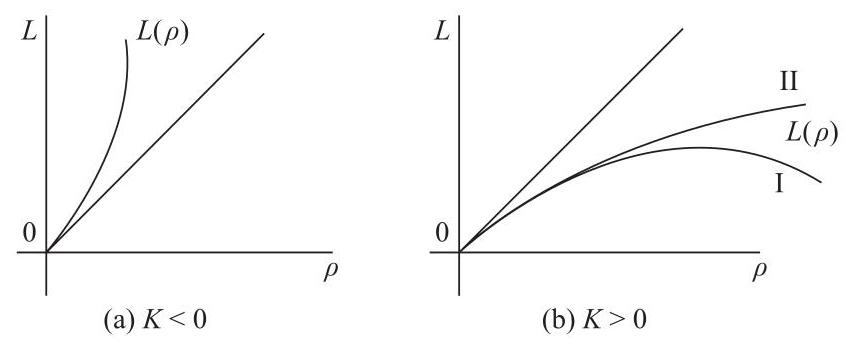
\includegraphics[max width=0.7\textwidth]{images/bo_d4b9jf3ef24c73e0334g_306_356_191_849_346_0.jpg}
\end{center}
\hspace*{3em} 

图 4-39. 法邻域中接近的测地线的展开.

\begin{center}
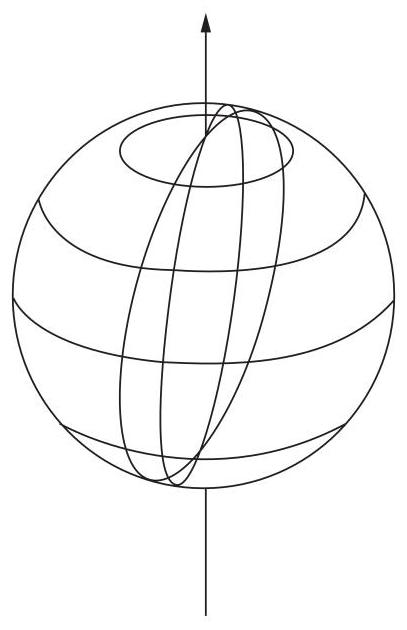
\includegraphics[max width=0.3\textwidth]{images/bo_d4b9jf3ef24c73e0334g_306_197_658_407_630_0.jpg}
\end{center}
\hspace*{3em} 

图 4-40

为此，我们首先注意到，在以 \(p \in  S\) 为中心的测地极坐标 \(\left( {\rho ,\theta }\right)\) 中， \(K\) 的表达式为

\[
K =  - \frac{{\left( \sqrt{G}\right) }_{\rho \rho }}{\sqrt{G}},
\]

因此

\[
\frac{{\partial }^{3}\left( \sqrt{G}\right) }{\partial {\rho }^{3}} =  - K{\left( \sqrt{G}\right) }_{\rho } - {K}_{\rho }\left( \sqrt{G}\right) .
\]

因此，回想一下

\[
\mathop{\lim }\limits_{{\rho  \rightarrow  0}}\sqrt{G} = 0
\]

我们得到

\[
- K\left( p\right)  = \mathop{\lim }\limits_{{\rho  \rightarrow  0}}\frac{{\partial }^{3}\sqrt{G}}{\partial {\rho }^{3}}.
\]

另一方面，通过定义 \(\sqrt{G}\) 及其相对于 \(\rho\) 在 \(p\) 处的导数(参见公式 (1))的极限值，我们可以写出

\[
\sqrt{G}\left( {\rho ,\theta }\right)  = \sqrt{G}\left( {0,\theta }\right)  + \rho {\left( \sqrt{G}\right) }_{\rho }\left( {0,\theta }\right)  + \frac{{\rho }^{2}}{2!}{\left( \sqrt{G}\right) }_{\rho \rho }\left( {0,\theta }\right)
\]

\[
+ \frac{{\rho }^{3}}{3!}{\left( \sqrt{G}\right) }_{\rho \rho \rho }\left( {0,\theta }\right)  + R\left( {\rho ,\theta }\right)
\]

其中

\[
\mathop{\lim }\limits_{{\rho  \rightarrow  0}}\frac{R\left( {\rho ,\theta }\right) }{{\rho }^{3}} = 0,
\]

在 \(\theta\) 中一致.将已知值代入上述表达式，我们得到

\[
\sqrt{G}\left( {\rho ,\theta }\right)  = \rho  - \frac{{\rho }^{3}}{3!}K\left( \rho \right)  + R.
\]

有了 \(\sqrt{G}\) 的这个值，我们计算半径为 \(\rho  = r\) 的测地圆的弧长 \(L\) :

\[
L = \mathop{\lim }\limits_{{\epsilon  \rightarrow  0}}{\int }_{0 + \epsilon }^{{2\pi } - \epsilon }\sqrt{G}\left( {r,\theta }\right) {d\theta } = {2\pi r} - \frac{\pi }{3}{r}^{3}K\left( p\right)  + {R}_{1},
\]

其中

\[
\mathop{\lim }\limits_{{r \rightarrow  0}}\frac{{R}_{1}}{{r}^{3}} = 0
\]

由此可知

\[
K\left( p\right)  = \mathop{\lim }\limits_{{r \rightarrow  0}}\frac{3}{\pi }\frac{{2\pi r} - L}{{r}^{3}},
\]

这提供了 \(K\left( p\right)\) 的内在解释，用测地圆 \({S}_{r}\left( p\right)\) 的半径 \(r\) (围绕 \(p\) )以及 \({S}_{r}\left( P\right)\) 和 \({\exp }_{p}^{-1}\left( {{S}_{r}\left( p\right) }\right)\) 的弧长 \(L\) 和 \({2\pi r}\) 来表示，分别表示.

通过上述过程可以轻松获得涉及由 \({S}_{r}\left( p\right)\) 界定的区域面积的 \(K\left( p\right)\) 的解释(参见练习 3).

作为测地极坐标的最后一个应用，我们将研究测地线的一些极小性质.测地线的一个基本性质是，局部上它最小化弧长.更准确地说，我们有

命题 4. 设 \(\mathrm{p}\) 是曲面 S 上的一个点.那么，存在 \(\mathrm{p}\) 的一个邻域 \(\mathrm{W} \subset  S\) ，使得如果 \(\gamma  : \mathrm{I} \rightarrow  \mathrm{W}\) 是一条参数化的测地线，且 \(\gamma \left( 0\right)  = \mathrm{p},\gamma \left( {\mathrm{t}}_{1}\right)  = \mathrm{q},{\mathrm{t}}_{1} \in  \mathrm{I}\) ，而 \(\alpha  : \left\lbrack  {0,{\mathrm{t}}_{1}}\right\rbrack   \rightarrow  S\) 是一条连接 \(\mathrm{p}\) 和 \(q\) 的参数化正则曲线，则有

\[
{l}_{\gamma } \leq  {l}_{\alpha }
\]

其中 \({l}_{\alpha }\) 表示曲线 \(\alpha\) 的长度.此外，如果 \({l}_{r} = {l}_{\alpha }\) ，则 \(\gamma\) 的轨迹与 \(\alpha\) 在 \(\mathrm{p}\) 和 \(\mathrm{q}\) 之间的轨迹重合.

证明.设 \(V\) 是 \(p\) 的一个法邻域，设 \(\bar{W}\) 是一个闭区域，由包含在 \(V\) 中的半径为 \(r\) 的测地圆界定.设 \(\left( {\rho ,\theta }\right)\) 是 \(\bar{W} - L\) 中以 \(p\) 为中心的测地极坐标.

\begin{center}
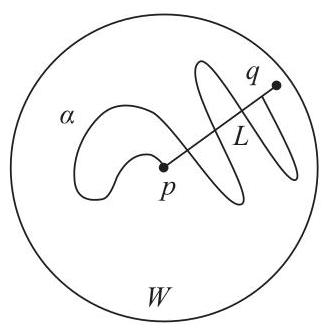
\includegraphics[max width=0.2\textwidth]{images/bo_d4b9jf3ef24c73e0334g_308_199_674_327_333_0.jpg}
\end{center}
\hspace*{3em} 

图 4-41

我们首先考虑 \(\alpha \left( \left\lbrack  {0,{t}_{1}}\right\rbrack  \right)  \subset  W\) 的情况(图 4-41).设 \(0 < {\beta }_{0} < \; {\beta }_{1} < {t}_{1}\) .由于 \(\alpha\) 具有有限长度，我们可以选择 \(L\) ，使得 \(\alpha \left( \left\lbrack  {{\beta }_{0},{\beta }_{1}}\right\rbrack  \right)\) 与 \(L\) 的交点为有限个，设为 \({\tau }_{1} < {\tau }_{2} < \cdots  < {\tau }_{k - 1}\) .令 \({\beta }_{0} = {\tau }_{0},{\beta }_{1} = {\tau }_{k}\) ，并在每个区间 \(\left( {{\tau }_{i},{\tau }_{i + 1}}\right)\) 、 \(i = 0,\ldots ,k - 1\) 中将 \(\alpha \left( t\right)  = \left( {\rho \left( t\right) ,\beta \left( t\right) }\right)\) 写为.

\[
\sqrt{{\left( {\rho }^{\prime }\right) }^{2} + G{\left( {\theta }^{\prime }\right) }^{2}} \geq  \sqrt{{\left( {\rho }^{\prime }\right) }^{2}}
\]

当且仅当 \({\theta }^{\prime } = 0\) ，即 \(\left( {{\tau }_{i},{\tau }_{i + 1}}\right)\) 中的 \(\theta  =\) 为常数时， \(\left( {{\tau }_{i},{\tau }_{i + 1}}\right)\) 中的等式成立.我们声称， \({\beta }_{0}\) 和 \({\beta }_{1}\) 之间的 \(\alpha\) 的长度大于或等于 \(\left| {\rho \left( {\beta }_{1}\right)  - \rho \left( {\beta }_{0}\right) }\right|\) ，并且当且仅当 \(\alpha\) 是具有参数 \(\rho \left( t\right)\) 的径向测地线 \(\theta  =\) 为常数时，等式成立，其中 \({\rho }^{\prime }\left( t\right)  > 0\) .

为了说明这一点，注意到这样的长度由(收敛的)不适定积分给出

\[
\mathop{\sum }\limits_{{i = 0}}^{{k + 1}}{\int }_{{\tau }_{i}}^{{\tau }_{i + 1}}\sqrt{{\left( {\rho }^{\prime }\right) }^{2} + G{\left( {\theta }^{\prime }\right) }^{2}}{dt} \geq  \mathop{\sum }\limits_{i}{\int }_{{\tau }_{i}}^{{\tau }_{i + 1}}\sqrt{{\left( {\rho }^{\prime }\right) }^{2}}{dt}
\]

\[
= \mathop{\sum }\limits_{i}{\int }_{{\tau }_{i}}^{{\tau }_{i + 1}}\left| {\rho }^{\prime }\right| {dt} \geq  \left| {\rho \left( {\beta }_{1}\right)  - \rho \left( {\beta }_{2}\right) }\right| .
\]

此外，当且仅当 \({\rho }^{\prime }\left( t\right)  > 0\) 和 \(\theta \left( t\right)  =\) 在每个区间 \(\left( {{\tau }_{i},{\tau }_{i + 1}}\right)\) 上为常数时，上述等式成立，即 \(\alpha \left( {\tau }_{i}\right)\) 和 \(\alpha \left( {\tau }_{i + 1}\right)\) 实际上在一条径向测地线上.这就证明了我们的论断.

命题 4 在 \(\alpha \left( \left\lbrack  {{p}_{0},{t}_{1}}\right\rbrack  \right)  \subset  \bar{W}\) 的情况下，通过令 \({\beta }_{0} \rightarrow  0\) 和 \({\beta }_{1} \rightarrow  {t}_{1}\) ，可以立即从上述论断中得出.

最后假设 \(\alpha \left( \left\lbrack  {0,{t}_{1}}\right\rbrack  \right)\) 没有完全包含在 \(\bar{W}\) 中.设 \({t}_{0} \in  \left\lbrack  {0,{t}_{1}}\right\rbrack\) 为 \(\alpha \left( {t}_{0}\right)  = x\) 属于 \(\bar{W}\) 边界的第一个值.设 \(\overline{\gamma }\) 为径向测地线 \({px}\) ，并设 \(\overline{\alpha }\) 为曲线 \(\alpha\) 在区间 \(\left\lbrack  {0,{t}_{0}}\right\rbrack\) 上的限制.那么显然 \({l}_{\alpha } \geq  {l}_{\alpha }\) (见图 4-42).

\begin{center}
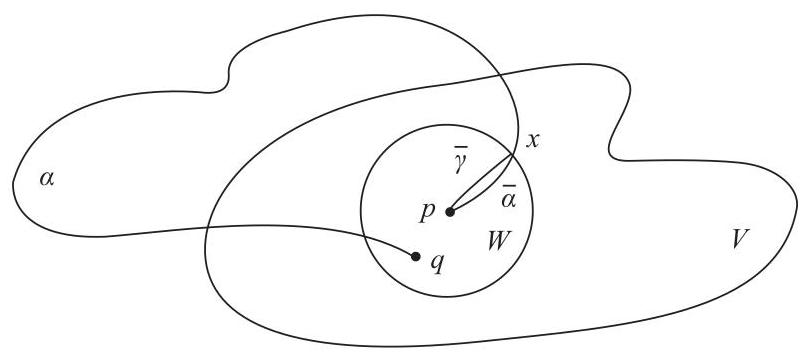
\includegraphics[max width=0.7\textwidth]{images/bo_d4b9jf3ef24c73e0334g_309_362_522_809_353_0.jpg}
\end{center}
\hspace*{3em} 

图 4-42

根据之前的论证， \({l}_{\overline{\alpha }} \geq  {l}_{\overline{\gamma }}\) .由于 \(q\) 是 \(\bar{W}\) 的内部点， \({l}_{\overline{\gamma }} > {l}_{\gamma }\) .我们得出结论， \({l}_{\alpha } > {l}_{\gamma }\) ，证明完毕.Q.E.D.

注3.为简化起见，我们已证明了该命题对正则曲线成立.然而，它对分段正则曲线(参见定义7，第4-4节)也成立；证明完全类似，留作练习.

注 4. 证明也表明，命题 4 的最后一个断言的逆命题成立.然而，这个逆命题不能推广到分段正则曲线.

前面的命题并非全局成立，球面的例子就说明了这一点.球面上两个非对径点可以通过两条长度不等的经线连接，只有较短的一条满足命题的结论.换句话说，测地线如果足够长，可能不是其端点之间的最短路径.然而，下面的命题表明，当一条正则曲线是其任意两点之间的最短路径时，这条曲线必然是一条测地线.

命题 5. 设 \(\alpha  : \mathrm{I} \rightarrow  S\) 是一条正则参数化曲线，其参数与弧长成比例.假设 \(\alpha\) 上任意两点 \(\mathrm{t},\tau  \in  \mathrm{I}\) 之间的弧长小于或等于连接 \(\alpha \left( \mathrm{t}\right)\) 和 \(\alpha \left( \tau \right)\) 的任意一条正则参数化曲线的弧长.则 \(\alpha\) 是一条测地线.

证明. 设 \({t}_{0} \in  I\) 是 \(I\) 上的任意一点，设 \(W\) 是由命题 4 给出的 \(\alpha \left( {t}_{0}\right)  = p\) 的邻域.设 \(q = \alpha \left( {t}_{1}\right)  \in  W\) .从命题 4 的等号情况可知， \(\alpha\) 在 \(\left( {{t}_{0},{t}_{1}}\right)\) 中是一条测地线.否则， \(\alpha\) 在 \({t}_{0}\) 和 \({t}_{1}\) 之间的长度将大于连接 \(\alpha \left( {t}_{0}\right)\) 和 \(\alpha \left( {t}_{1}\right)\) 的径向测地线，这与假设矛盾.由于 \(\alpha\) 是正则的，我们通过连续性可知， \(\alpha\) 在 \({t}_{0}\) 中仍然是一条测地线.证毕.

\exerciseline

1. 证明在常曲率的曲面上，测地圆具有常测地曲率.

2. 证明在测地极坐标 \(\left( {E = 1,F = 0}\right)\) 中，测地线的方程由下式给出

\[
{\rho }^{\prime \prime } - \frac{1}{2}{G}_{\rho }{\left( {\theta }^{\prime }\right) }^{2} = 0
\]

\[
{\theta }^{\prime \prime } + \frac{{G}_{\rho }}{G}{\rho }^{\prime }{\theta }^{\prime } + \frac{1}{2}\frac{{G}_{\theta }}{G}{\left( {\theta }^{\prime }\right) }^{2} = 0.
\]

3. 如果 \(p\) 是正则曲面 \(S\) 上的一个点，证明

\[
K\left( p\right)  = \mathop{\lim }\limits_{{r \rightarrow  0}}\frac{12}{\pi }\frac{\pi {r}^{2} - A}{{r}^{4}},
\]

其中 \(K\left( p\right)\) 是 \(S\) 在 \(p,r\) 处的斯曲率， \({S}_{r}\left( p\right)\) 是以 \(p\) 为中心的测地圆的半径， \(A\) 是由 \({S}_{r}\left( p\right)\) 围成的区域的面积.

4. 证明在以 \(p\) 为中心的法坐标系中，所有克里斯托费尔符号在 \(p\) 处都为零.

5. 对于下面给出的曲面对，哪些存在局部等距映射？

a. 回转环面和圆锥面.

b. 圆锥面和球面.

c. 圆锥面和圆柱面.

6. 设 \(S\) 是一个曲面， \(p\) 是 \(S\) 上的一个点， \({S}^{1}\left( p\right)\) 是围绕 \(p\) 的一个测地圆，足够小以包含在法邻域内.设 \(r\) 和 \(s\) 是 \({S}^{1}\left( p\right)\) 上的两个点， \(C\) 是 \({S}^{1}\left( p\right)\) 上介于 \(r\) 和 \(s\) 之间的弧.考虑曲线 \({\exp }_{p}^{-1}\left( C\right)  \subset  {T}_{p}\left( S\right)\) .证明 \({S}^{1}\left( p\right)\) 可以选择得足够小，使得

a. 若 \(K > 0\) ，则 \(l\left( {{\exp }_{p}^{-1}\left( C\right) }\right)  > l\left( C\right)\) ，其中 \(l\left( \right)\) 表示相应曲线的弧长.

b. 若 \(K < 0\) ，则 \(l\left( {{\exp }_{p}^{-1}\left( C\right) }\right)  < l\left( C\right)\) .

7. 设 \(\left( {\rho ,\theta }\right)\) 是曲面 \(\left( {E = 1,F = 0}\right)\) 上的测地极坐标系，设 \(\gamma \left( {\rho \left( s\right) ,\theta \left( s\right) }\right)\) 是一条与曲线 \(\theta  =\) 常数成角 \(\varphi \left( s\right)\) 的测地线.为明确起见，曲线 \(\theta  =\) 常数按 \(\rho\) 增大方向定向，并且 \(\varphi\) 从 \(\theta  =\) 常数测量到 \(\gamma\) ，方向由参数化 \(\left( {\rho ,\theta }\right)\) 给出.证明:

\[
\frac{d\varphi }{ds} + {\left( \sqrt{G}\right) }_{\rho }\frac{d\theta }{ds} = 0.
\]

*8. (“小”测地三角形内角和的高斯定理.)设 \(\Delta\) 是曲面 \(S\) 上的一个测地三角形(即其边是测地线的段).假设 \(\Delta\) 足够小，可以包含在其某个顶点的法域内.直接证明(即不使用高斯-博内定理)以下等式成立:

\[
{\iint }_{\Delta }{KdA} = \left( {\mathop{\sum }\limits_{{i = 1}}^{3}{\alpha }_{i}}\right)  - \pi ,
\]

其中 \(K\) 是 \(S\) 的高斯曲率，而 \(0 < {\alpha }_{i} < \pi ,i = 1,2,3\) 是三角形 \(\Delta\) 的内角.

9. (测地圆的局部等周不等式.)设 \(p \in  S\) ，且 \({S}_{r}\left( p\right)\) 是以 \(p\) 为中心、半径为 \(r\) 的测地圆.设 \(L\) 是 \({S}_{r}\left( p\right)\) 的弧长， \(A\) 是由 \({S}_{r}\left( p\right)\) 围成的区域的面积.证明:

\[
{4\pi A} - {L}^{2} = {\pi }^{2}{r}^{4}K\left( p\right)  + R,
\]

其中 \(K\left( p\right)\) 是 \(S\) 在 \(p\) 处的高斯曲率，而

\[
\mathop{\lim }\limits_{{r \rightarrow  0}}\frac{R}{{r}^{4}} = 0
\]

因此，如果 \(K\left( p\right)  > 0\) (或 \(< 0\) )且 \(r\) 很小，则 \({4\pi A} - {L}^{2} > 0\) (或 \(< 0\) ).(比较第 1-7 节的等周不等式.)

10. 设 \(S\) 是一个连通曲面，设 \(\varphi ,\psi  : S \rightarrow  S\) 是 \(S\) 的两个等距映射.假设存在一点 \(p \in  S\) 使得对于所有 \(v \in  {T}_{p}\left( S\right)\) 都有 \(\varphi \left( p\right)  = \psi \left( p\right)\) 和 \(d{\varphi }_{p}\left( v\right)  = d{\psi }_{p}\left( v\right)\) .证明对于所有 \(q \in  S\) 都有 \(\varphi \left( q\right)  = \psi \left( q\right)\) .

11. 如果对于 \({S}_{1}\) 的每条测地线 \(C \subset  {S}_{1}\) ，正则曲线 \(\varphi \left( C\right)  \subset  {S}_{2}\) 都是 \({S}_{2}\) 的测地线，则称微分同胚 \(\varphi  : {S}_{1} \rightarrow  {S}_{2}\) 为测地映射.如果 \(U\) 是 \(p \in  {S}_{1}\) 的一个邻域，则称 \(\varphi  : U \rightarrow  {S}_{2}\) 在 \(p\) 中是局部测地映射，如果存在 \({S}_{2}\) 中 \(\varphi \left( p\right)\) 的一个邻域 \(V\) ，使得 \(\varphi  : U \rightarrow  V\) 是一个测地映射.

a. 证明如果 \(\varphi  : {S}_{1} \rightarrow  {S}_{2}\) 既是测地映射又是共形映射，则 \(\varphi\) 是相似映射；即，

\[
\langle v,w{\rangle }_{p} = \lambda {\left\langle  d{\varphi }_{p}\left( v\right) ,d{\varphi }_{p}\left( w\right) \right\rangle  }_{\varphi \left( p\right) },\;p \in  {S}_{1},v,w \in  {T}_{p}\left( {S}_{1}\right) ,
\]

其中 \(\lambda\) 是常数.

b. 令 \({S}^{2} = \left\{  {\left( {x,y,z}\right)  \in  {R}^{3};{x}^{2} + {y}^{2} + {z}^{2} = 1}\right\}\) 为单位球面， \({S}^{ - } = \; \{ \left( {x,y,z}\right)  \in  {S}^{2};z < 0\}\) 为其下半球面， \(P\) 为平面 \(z =  - 1\) .证明映射(中心投影) \(\varphi  : {S}^{ - } \rightarrow  P\) 将点 \(p \in  {S}^{ - }\) 映射到 \(P\) 与连接 \(p\) 和 \({S}^{2}\) 的中心的直线相交的点，是一个测地映射.

*c. 证明对于任意 \(p \in  S\) ，常曲率曲面都允许一个局部测地映射到平面.

12. (Beltrami 定理.)在习题 11 的第 \(\mathrm{c}\) 部分，我们证明了常曲率 \(K\) 的曲面 \(S\) 对于任意 \(p \in  S\) 都允许一个到平面的局部测地映射.为了证明其逆命题(Beltrami 定理)——如果一个正则连通曲面 \(S\) 对于任意 \(\mathrm{p} \in  S\) 都允许一个到平面的局部测地映射，则 \(S\) 的曲率为常数，应证明以下命题:

a. 如果 \(v = v\left( u\right)\) 是一条测地线，在由 \(\left( {u,v}\right)\) 参数化的曲面(不与 \(u =\) const. 重合)的坐标邻域中，则

\[
\frac{{d}^{2}v}{d{u}^{2}} = {\mathbf{\Gamma }}_{22}^{1}{\left( \frac{dv}{du}\right) }^{3} + \left( {2{\mathbf{\Gamma }}_{12}^{1} - {\mathbf{\Gamma }}_{22}^{2}}\right) {\left( \frac{dv}{du}\right) }^{2} + \left( {{\mathbf{\Gamma }}_{11}^{1} - 2{\mathbf{\Gamma }}_{12}^{2}}\right) \frac{dv}{du} - {\mathbf{\Gamma }}_{11}^{2}.
\]

*b. 如果 \(S\) 允许一个点 \(p \in  S\) 的邻域 \(V\) 到平面 \({R}^{2}\) 的局部测地映射 \(\varphi  : V \rightarrow  {R}^{2}\) ，则可以对邻域 \(V\) 进行参数化，使得 \(\left( {u,v}\right)\) 满足:

\[
{\mathbf{\Gamma }}_{22}^{1} = {\mathbf{\Gamma }}_{11}^{2} = 0,\;{\mathbf{\Gamma }}_{22}^{2} = 2{\mathbf{\Gamma }}_{12}^{1},\;{\mathbf{\Gamma }}_{11}^{1} = 2{\mathbf{\Gamma }}_{12}^{2}.
\]

*c. 如果存在一个邻域 \(V\) 的 \(p \in  S\) 到平面的测地映射，则 \(V\) 中的曲率 \(K\) 满足关系式

\[
{KE} = {\Gamma }_{12}^{2}{\Gamma }_{12}^{2} - {\left( {\Gamma }_{12}^{2}\right) }_{u} \tag{a}
\]

\[
{KF} = {\mathbf{\Gamma }}_{12}^{1}{\mathbf{\Gamma }}_{12}^{2} - {\left( {\mathbf{\Gamma }}_{12}^{2}\right) }_{v} \tag{b}
\]

\[
{KG} = {\mathbf{\Gamma }}_{12}^{1}{\mathbf{\Gamma }}_{12}^{1} - {\left( {\mathbf{\Gamma }}_{12}^{1}\right) }_{v} \tag{c}
\]

\[
{KF} = {\mathbf{\Gamma }}_{12}^{2}{\mathbf{\Gamma }}_{12}^{1} - {\left( {\mathbf{\Gamma }}_{12}^{1}\right) }_{u} \tag{d}
\]

*d. 如果存在一个邻域 \(V\) 的 \(p \in  S\) 到平面的测地映射，则 \(V\) 中的曲率 \(K\) 是常数.

e. 利用上述结果和连通性的标准论证，证明 Beltrami 定理.

13. (全 সম্পর্কিত群.) 令 \(S\) 为一个正则曲面，令 \(p \in  S\) .对于每条分段正则参数化曲线 \(\alpha  : \left\lbrack  {0,l}\right\rbrack   \rightarrow  S\) ，其中 \(\alpha \left( 0\right)  = \alpha \left( l\right)  = \; p\) ，令 \({P}_{\alpha } : {T}_{p}\left( S\right)  \rightarrow  {T}_{p}\left( S\right)\) 为映射，它将 \(v \in  {T}_{p}\left( S\right)\) 映射到沿 \(\alpha\) 平行移动回到 \(p\) 的点.根据 4-4 节的命题 1， \({P}_{\alpha }\) 是 \({T}_{p}\left( S\right)\) 的一个线性等距映射.如果 \(\beta  : \left\lbrack  {l,\bar{l}}\right\rbrack\) 是另一条分段正则参数化曲线，其中 \(\beta \left( \dot{l}\right)  = \beta \left( \bar{l}\right)  = p\) ，则定义曲线 \(\beta  \circ  \alpha  : \left\lbrack  {0,\bar{l}}\right\rbrack   \rightarrow  S\) ，通过依次先运行 \(\alpha\) 再运行 \(\beta\) ；也就是说，如果 \(s \in  \left\lbrack  {0,l}\right\rbrack\) ，则 \(\beta  \circ  \alpha \left( s\right)  = \alpha \left( s\right)\) ，如果 \(s \in  \left\lbrack  {l,\bar{l}}\right\rbrack\) ，则 \(\beta  \circ  \alpha \left( s\right)  = \beta \left( s\right)\) .

a. 考虑集合

\[
{H}_{p}\left( S\right)  = \left\{  {{P}_{\alpha } : {T}_{p}\left( S\right)  \rightarrow  {T}_{p}\left( S\right) \text{ ; all }\alpha \text{ joining }p\text{ to }p}\right\}  \text{ , }
\]

其中 \(\alpha\) 是分段正则的.在该集合中定义运算 \({P}_{\beta } \circ  {P}_{\alpha } = \; {P}_{\beta  \circ  \alpha }\) ；也就是说， \({P}_{\beta } \circ  {P}_{\alpha }\) 是先执行 \({P}_{\alpha }\) 再执行 \({P}_{\beta }\) 的通常复合运算.证明，通过此运算， \({H}_{p}\left( S\right)\) 是一个群(实际上，是 \({T}_{p}\left( S\right)\) 的线性等距群的一个子群). \({H}_{p}\left( S\right)\) 被称为 \(S\) 在 \(p\) 处的全 সম্পর্কিত群.

b. 表明，与盘同胚且具有 \(K \equiv  0\) 的曲面上任意点的全 সম্পর্কিত群退化为恒等映射.

c. 证明，如果 \(S\) 是连通的，则在两个任意点 \(p,q \in  S\) 处，全 সম্পর্কিত群 \({H}_{p}\left( S\right)\) 和 \({H}_{q}\left( S\right)\) 是同构的.因此，我们可以讨论曲面的(抽象)全 সম্পর্কিত群.

d. 证明，球面的全 সম্পর্কিত群同构于 \(2 \times  2\) 旋转矩阵群(参见练习 22，4-4 节).

\section*{4-7. 测地线的进一步性质；凸邻域 \({}^{ \dagger  }\)}

在本节中，我们将展示测地线的一些事实(特别是 4-4 节的命题 5)如何从向量场存在性、唯一性和初值依赖性的普遍定理中得出.

在参数化 \(\mathbf{x}\left( {u,v}\right)\) 下的测地线由以下系统给出:

(1)
\[
{u}^{\prime \prime } + {\mathbf{\Gamma }}_{11}^{1}{\left( {u}^{\prime }\right) }^{2} + 2{\mathbf{\Gamma }}_{12}^{1}{u}^{\prime }{v}^{\prime } + {\mathbf{\Gamma }}_{22}^{1}{\left( {v}^{\prime }\right) }^{2} = 0,
\]

\[
{v}^{\prime \prime } + {\mathbf{\Gamma }}_{11}^{2}{\left( {u}^{\prime }\right) }^{2} + 2{\mathbf{\Gamma }}_{12}^{2}{u}^{\prime }{v}^{\prime } + {\mathbf{\Gamma }}_{22}^{2}{\left( {v}^{\prime }\right) }^{2} = 0,
\]

其中 \({\mathbf{\Gamma }}_{ij}^{k}\) 是局部坐标 \(u\) 和 \(v\) 的函数.通过令 \({u}^{\prime } = \xi\) 和 \({v}^{\prime } = \eta\) ，我们可以将上述系统写成一般形式:

\[
{\xi }^{\prime } = {F}_{1}\left( {u,v,\xi ,\eta }\right) ,
\]

(2)
\[
{\eta }^{\prime } = {F}_{2}\left( {u,v,\xi ,\eta }\right)
\]

\[
{u}^{\prime } = {F}_{3}\left( {u,v,\xi ,\eta }\right) ,
\]

\[
{v}^{\prime } = {F}_{4}\left( {u,v,\xi ,\eta }\right) ,
\]



†本节在初读时可以跳过.然而，命题 1 和 2(它们的陈述可以在不阅读本节的情况下理解)在第 5 章中使用.



其中 \({F}_{3}\left( {u,v,\xi ,\eta }\right)  = \xi ,{F}_{4}\left( {u,v,\xi ,\eta }\right)  = \eta\) .

使用以下记法很方便: \(\left( {u,v,\xi ,\eta }\right)\) 表示一个 \({R}^{4}\) 的点，它将被看作是笛卡尔积 \({R}^{4} = {R}^{2} \times  {R}^{2}\) ； \(\left( {u,v}\right)\) 表示第一个因子中的一个点，而 \(\left( {\xi ,\eta }\right)\) 表示第二个因子中的一个点.

系统 (2) 等价于 \({R}^{4}\) 的一个开集中的向量场，该向量场以完全类似于 \({R}^{2}\) 中向量场的方式定义(参见第 3-4 节).轨迹的存在性和唯一性定理(第 3-4 节定理 1)在此情况下仍然成立(实际上，该定理适用于 \({R}^{n}\) ；参见 S. Lang, Analysis I, Addison-Wesley, Reading, Mass., 1968, pp. 383-386)，其表述如下:

给定 \(U \subset  {R}^{4}\) 的一个开集中的系统 (2) 和一个点

\[
\left( {{\mathrm{u}}_{0},{\mathrm{v}}_{0},{\xi }_{0},{\eta }_{0}}\right)  \in  \mathrm{U}
\]

存在一个唯一的轨迹 \(\alpha  : \left( {-\epsilon ,\epsilon }\right)  \rightarrow  \mathrm{U}\) ，属于 \(\mathrm{{Eq}}\) .(2)，且

\[
\alpha \left( 0\right)  = \left( {{\mathrm{u}}_{0},{\mathrm{v}}_{0},{\xi }_{0},{\eta }_{0}}\right) .
\]

为了将此结果应用于一个正则曲面 \(S\) ，我们应该注意到，给定一个在 \(p \in  S\) 中的参数化 \(\mathbf{x}\left( {u,v}\right)\) ，坐标邻域 \(V\) ，点对集 \(\left( {q,v}\right) ,q \in  V,v \in  {T}_{q}\left( S\right)\) 可以被识别为一个开集 \(V \times  {R}^{2} = \; U \subset  {R}^{4}\) .为此，我们通过基 \(\left\{  {{\mathbf{x}}_{u},{\mathbf{x}}_{v}}\right\}\) 将每个 \({T}_{q}\left( S\right) ,q \in  V\) 与 \({R}^{2}\) 进行识别.每当我们谈论点对集 \(\left( {q,v}\right)\) 中的可微性和连续性时，我们指的是由这种识别引起的微可微性和连续性.

假设上述定理，第 4-4 节命题 5 的证明是微不足道的.事实上，在 \(p \in  S\) 中的参数化 \(\mathbf{x}\left( {u,v}\right)\) 下测地线的方程在 \(U \subset  {R}^{4}\) 中产生一个形式为 (2) 的系统.基本定理因此意味着，给定一个点 \(q = \left( {{u}_{0},{v}_{0}}\right)  \in  V\) 和一个非零切向量 \(v = \; \left( {{\xi }_{0},{\eta }_{0}}\right)  \in  {T}_{q}\left( S\right)\) ，存在一个唯一的参数化测地线

\[
\gamma  = \pi  \circ  \alpha  : \left( {-\epsilon ,\epsilon }\right)  \rightarrow  V
\]

在 \(V\) 中(其中 \(\pi \left( {q,v}\right)  = q\) 是投影 \(V \times  {R}^{2} \rightarrow  V\) ).

由式 (2) 定义的向量场关于初值条件的依赖性定理也很重要.它与 \({R}^{2} :\) 的向量场的情况基本相同.给定一点 \(\mathrm{p} = \left( {{\mathrm{u}}_{0},{\mathrm{v}}_{0},{\xi }_{0},{\eta }_{0}}\right)  \in  \mathrm{U}\) ，存在 \(\mathrm{p}\) 的邻域 \(\mathrm{V} = {\mathrm{V}}_{1} \times  {\mathrm{V}}_{2}\) (其中 \({\mathrm{V}}_{1}\) 是 \(\left( {{\mathrm{u}}_{0},{\mathrm{v}}_{0}}\right)\) 的邻域， \({\mathrm{V}}_{2}\) 是 \(\left( {{\xi }_{0},{\eta }_{0}}\right)\) 的邻域)、一个开区间 \(\mathrm{I}\) 和一个可微映射 \(\alpha  : \mathrm{I} \times  {\mathrm{V}}_{1} \times  {\mathrm{V}}_{2} \rightarrow  \mathrm{U}\) ，使得对于固定的 \(\left( {\mathrm{u},\mathrm{v},\xi ,\eta }\right)  = \left( {\mathrm{q},\mathrm{v}}\right)  \in  \mathrm{V}\) ，则 \(\alpha \left( {\mathrm{t},\mathrm{q},\mathrm{v}}\right) ,\mathrm{t} \in  \mathrm{I}\) 是通过 \(\left( {\mathrm{q},\mathrm{v}}\right)\) 的 (2) 的轨迹.

为了将此陈述应用于正则曲面 \(S\) ，我们在 \(p \in  S\) 中引入一个参数化，其坐标邻域为 \(V\) ，并像上面一样，将对 \(\left( {q,v}\right) ,q \in  V,v \in  {T}_{q}\left( S\right)\) 与 \(V \times  {R}^{2}\) 的识别.以对 \(\left( {p,0}\right)\) 作为初值条件，我们得到一个区间 \(\left( {-{\epsilon }_{2},{\epsilon }_{2}}\right)\) 、 \(S\) 中 \(p\) 的邻域 \({V}_{1} \subset  V\) 、 \({R}^{2}\) 中原点的邻域 \({V}_{2}\) 和一个可微映射

\[
\gamma  : \left( {-{\epsilon }_{2},{\epsilon }_{2}}\right)  \times  {V}_{1} \times  {V}_{2} \rightarrow  V
\]

使得如果 \(\left( {q,v}\right)  \in  {V}_{1} \times  {V}_{2},v \neq  0\) ，则曲线

\[
t \rightarrow  \gamma \left( {t,q,v}\right) ,\;t \in  \left( {-{\epsilon }_{2},{\epsilon }_{2}}\right) ,
\]

是满足 \(\gamma \left( {0,q,v}\right)  = q,{\gamma }^{\prime }\left( {0,q,v}\right)  = v\) 的 \(S\) 的测地线，并且如果 \(v = 0\) ，则该曲线简化为点 \(q\) .这里 \(\gamma  = \pi  \circ  \alpha\) ，其中 \(\pi \left( {q,v}\right)  = q\) 是投影 \(U = V \times  {R}^{2} \rightarrow  V\) ，而 \(\alpha\) 是上面给出的映射.

回到曲面上，集合 \({V}_{1} \times  {V}_{2}\) 的形式为

\[
\left\{  {\left( {q,v}\right) ,q \in  {V}_{1},v \in  {V}_{q}\left( 0\right)  \subset  {T}_{q}\left( S\right) }\right\}  ,
\]

其中 \({V}_{q}\left( 0\right)\) 表示 \({T}_{q}\left( S\right)\) 中原点的邻域.因此，如果我们把 \(\gamma\) 限制在 \(\left( {-{\epsilon }_{2},{\epsilon }_{2}}\right)  \times  \{ p\}  \times  {V}_{2}\) 上，我们可以选择 \(\{ p\}  \times  {V}_{2} = {B}_{{\epsilon }_{1}} \subset  {T}_{p}\left( S\right)\) ，并得到

定理 1. 给定 \(\mathrm{p} \in  S\) ，存在数 \({\epsilon }_{1} > 0,{\epsilon }_{2} > 0\) 和一个可微映射

\[
\gamma  : \left( {-{\epsilon }_{2},{\epsilon }_{2}}\right)  \times  {\mathrm{B}}_{{\epsilon }_{1}} \rightarrow  S,\;{\mathrm{B}}_{{\epsilon }_{1}} \subset  {\mathrm{T}}_{\mathrm{p}}\left( S\right)
\]

使得对于 \(\mathrm{v} \in  {\mathrm{B}}_{{\epsilon }_{1}},\mathrm{v} \neq  0,\mathrm{t} \in  \left( {-{\epsilon }_{2},{\epsilon }_{2}}\right)\) ，曲线 \(\mathrm{t} \rightarrow  \gamma \left( {\mathrm{t},\mathrm{v}}\right)\) 是 \(S\) 关于 \(\gamma \left( {0,\mathrm{v}}\right)  = \mathrm{p},{\gamma }^{\prime }\left( {0,\mathrm{v}}\right)  = \mathrm{v}\) 的测地线，并且对于 \(\mathrm{v} = 0,\gamma \left( {\mathrm{t},0}\right)  = \mathrm{p}\) .

该结果用于 4-6 节命题 1 的证明中.

上述定理对应于 \(p\) 固定 的情况.为了处理一般情况，我们用 \({B}_{r}\left( q\right)\) 表示由半径为 \(r\) 、中心为 \(q\) 的(小的)测地圆所界定的区域，并用 \({\bar{B}}_{r}\left( q\right)\) 表示 \({B}_{r}\left( q\right)\) 及其边界的并集.

设 \(\epsilon  > 0\) 使得 \({\bar{B}}_{\epsilon }\left( p\right)  \subset  {V}_{1}\) .设 \({B}_{\delta \left( q\right) }\left( 0\right)  \subset  {\bar{V}}_{q}\left( 0\right)\) 是由 \({V}_{q}\left( 0\right)\) 及其极限点组成的集合 \({\bar{V}}_{q}\left( 0\right)\) 中的最大开圆盘，并设 \({\epsilon }_{1} = \inf \delta \left( q\right) ,q \in  {\bar{B}}_{\epsilon }\left( p\right)\) .显然， \(\epsilon  > 0\) .因此，集合

\[
\mathfrak{U} = \left\{  {\left( {q,v}\right) ;q \in  {B}_{\epsilon }\left( p\right) ,v \in  {B}_{{\epsilon }_{1}}\left( 0\right)  \subset  {T}_{q}\left( S\right) }\right\}
\]

包含在 \({V}_{1} \times  {V}_{2}\) 中，并且我们得到

定理 1a.给定 \(\mathrm{p} \in  S\) ，存在正数 \(\epsilon ,{\epsilon }_{1},{\epsilon }_{2}\) 和一个可微映射

\[
\gamma  : \left( {-{\epsilon }_{2},{\epsilon }_{2}}\right)  \times  \mathfrak{U} \rightarrow  S,
\]

其中

\[
\mathfrak{U} = \left\{  {\left( {\mathrm{q},\mathrm{v}}\right) ;\mathrm{q} \in  {\mathrm{B}}_{\epsilon }\left( \mathrm{p}\right) ,\mathrm{v} \in  {\mathrm{B}}_{{\epsilon }_{1}}\left( 0\right)  \subset  {\mathrm{T}}_{\mathrm{q}}\left( S\right) }\right\}  ,
\]

使得 \(\gamma \left( {\mathrm{t},\mathrm{q},0}\right)  = \mathrm{q}\) ，并且对于 \(\mathrm{v} \neq  0\) ，曲线

\[
\mathrm{t} \rightarrow  \gamma \left( {\mathrm{t},\mathrm{q},\mathrm{v}}\right) ,\;\mathrm{t} \in  \left( {-{\epsilon }_{2},{\epsilon }_{2}}\right)
\]

是 \(S\) 关于 \(\gamma \left( {0,\mathrm{q},\mathrm{v}}\right)  = \mathrm{q},{\gamma }^{\prime }\left( {0,\mathrm{q},\mathrm{v}}\right)  = \mathrm{v}\) 的测地线.

让我们应用定理 1a 来获得以下关于法范数存在的精炼结果.

命题 1.给定 \(\mathrm{p} \in  S\) ，存在 \(S\) 中 \(\mathrm{p}\) 的一个邻域 \(\mathrm{W}\) 和一个数 \(\delta  > 0\) ，使得对于每一个 \(\mathrm{q} \in  \mathrm{W},{\exp }_{\mathrm{q}}\) ， 是 \({\mathrm{B}}_{\delta }\left( 0\right)  \subset  {\mathrm{T}}_{\mathrm{q}}\left( S\right)\) 上的一个微分同胚且 \({\exp }_{\mathrm{q}}\left( {{\mathrm{B}}_{\delta }\left( 0\right) }\right)  \supset  \mathrm{W}\) ；也就是说， \(\mathrm{W}\) 是其所有点的法范数邻域.

证明. 令 \(V\) 为 \(p\) 的一个坐标邻域. 令 \(\epsilon ,{\epsilon }_{1},{\epsilon }_{2}\) 和 \(\gamma  : \left( {-{\epsilon }_{1},{\epsilon }_{2}}\right)  \times  \mathfrak{U} \rightarrow  V\) 如定理 1a 所述. 通过选择 \({\epsilon }_{1} < {\epsilon }_{2}\) , 我们可以确保 \(\left( {q,v}\right)  \in  \mathfrak{U},{\exp }_{q}\left( v\right)  = \gamma \left( {\left| v\right| ,q,\frac{v}{\left| v\right| }}\right)\) 有定义. 因此, 我们可以定义一个可微映射 \(\varphi  : \mathfrak{U} \rightarrow  V \times  V\) 如下:

\[
\varphi \left( {q,v}\right)  = \left( {q,{\exp }_{q}\left( v\right) }\right) .
\]

我们首先证明 \({d\varphi }\) 在 \(\left( {p,0}\right)\) 处是非奇异的. 为此, 我们研究 \(\varphi\) 如何变换 \(\mathfrak{U}\) 中的曲线, 这些曲线由下式给出:

\[
t \rightarrow  \left( {p,{tw}}\right) ,\;t \rightarrow  \left( {\alpha \left( t\right) ,0}\right) ,
\]

其中 \(w \in  {T}_{p}\left( S\right)\) 和 \(\alpha \left( t\right)\) 是 \(S\) 中的一条曲线, 且满足 \(\alpha \left( 0\right)  = p\) . 注意到这些曲线在 \(t = 0\) 处的切向量分别是 \(\left( {0,w}\right)\) 和 \(\left( {{\alpha }^{\prime }\left( 0\right) ,0}\right)\) . 因此,

\[
d{\varphi }_{\left( p,0\right) }\left( {0,w}\right)  = {\left. \frac{d}{dt}\left( p,{\exp }_{p}\left( wt\right) \right) \right| }_{t = 0} = \left( {0,w}\right) ,
\]

\[
{\left. d{\varphi }_{\left( p,0\right) }\left( {\alpha }^{\prime }\left( 0\right) ,0\right)  = \frac{d}{dt}\left( \alpha \left( t\right) ,{\exp }_{\alpha \left( t\right) }\left( 0\right) \right) \right| }_{t = 0} = \left( {{\alpha }^{\prime }\left( 0\right) ,{\alpha }^{\prime }\left( 0\right) }\right) ,
\]

并且 \(d{\varphi }_{\left( p,0\right) }\) 将线性无关向量映射为线性无关向量. 因此, \(d{\varphi }_{\left( p,0\right) }\) 是非奇异的.

由此可知, 我们可以应用反函数定理, 并得出存在 \(\mathfrak{U}\) 中 \(\left( {p,0}\right)\) 的一个邻域 \(\mathfrak{V}\) , 使得 \(\varphi\) 将 \(\mathfrak{V}\) 微分同胚地映射到 \(V \times  V\) 中 \(\left( {p,p}\right)\) 的一个邻域. 令 \(U \subset  {B}_{\epsilon }\left( p\right)\) 和 \(\delta  > 0\) 满足:

\[
\mathfrak{V} = \left\{  {\left( {q,v}\right)  \in  \mathfrak{U};q \in  U,v \in  {B}_{\delta }\left( 0\right)  \subset  {T}_{q}\left( S\right) }\right\}  .
\]

最后，设 \(W \subset  U\) 是 \(p\) 的一个邻域，使得 \(W \times  W \subset  \varphi \left( \mathfrak{V}\right)\) .

我们声称由此得到的 \(\delta\) 和 \(W\) 满足定理的陈述. 事实上, 由于 \(\varphi\) 在 \(\mathfrak{V},{\exp }_{q}\) 中是微分同胚的, \({B}_{\delta }\left( 0\right)\) 是微分同胚的, \(q \in  W\) . 此外, 如果 \(q \in  W\) , 那么

\[
\varphi \left( {\{ q\}  \times  {B}_{\delta }\left( 0\right) }\right)  \supset  \{ q\}  \times  W,
\]

并且, 根据 \(\varphi ,{\exp }_{q}\left( {{B}_{\delta }\left( 0\right) }\right)  \supset  W\) 的定义.Q.E.D.

注记 1. 从前面的命题可知，给定两点 \({q}_{1},{q}_{2} \in  W\) ，存在一条长度小于 \(\delta\) 的唯一测地线 \(\gamma\) 连接 \({q}_{1}\) 和 \({q}_{2}\) .此外，证明也表明 \(\gamma\) 在以下意义上“可微地依赖”于 \({q}_{1}\) 和 \({q}_{2}\) :给定 \(\left( {{q}_{1},{q}_{2}}\right)  \in  W \times  W\) ，确定了一个唯一的 \(v \in  {T}_{{q}_{1}}\left( S\right)\) (精确地说，由 \({\varphi }^{-1}\left( {{q}_{1},{q}_{2}}\right)  = \left( {{q}_{1},v}\right)\) 给出的 \(v\) )，它可微地依赖于 \(\left( {{q}_{1},{q}_{2}}\right)\) 并且满足 \({\gamma }^{\prime }\left( 0\right)  = v\) .

前面结果的一个应用是证明局部最小化弧长的曲线不可能是“断开的”.更精确地说，我们有

命题 2. 令 \(\alpha  : \mathrm{I} \rightarrow  S\) 为一条参数化、分段正则曲线，使得在每段正则弧上，参数与弧长成比例.假设任意两点之间的弧长小于或等于连接这两点的任意一条参数化正则曲线的弧长.则 \(\alpha\) 是一条测地线；特别地， \(\alpha\) 在处处正则.

证明. 令 \(0 = {t}_{0} \leq  {t}_{1} \leq  \cdots  \leq  {t}_{k} \leq  {t}_{k + 1} = l\) 为 \(\left\lbrack  {0,l}\right\rbrack   = I\) 的一个细分，使得 \(\alpha  \mid  \left\lbrack  {{t}_{i},{t}_{i + 1}}\right\rbrack  ,i = 0,\ldots ,k\) 是正则的.根据第 4-6 节的命题 5， \(\alpha\) 在 \(\left( {{t}_{i},{t}_{i + 1}}\right)\) 的点处是测地线.为了证明 \(\alpha\) 在 \({t}_{i}\) 中是测地线，考虑由第 1 命题给出的 \(\alpha \left( {t}_{i}\right)\) 的邻域 \(W\) .令 \({q}_{1} = \alpha \left( {{t}_{i} - \epsilon }\right) ,{q}_{2} = \; \alpha \left( {{t}_{i} + \epsilon }\right) ,\epsilon  > 0\) 为 \(W\) 中的两点，令 \(\gamma\) 为连接 \({q}_{1}\) 和 \({q}_{2}\) 的 \({B}_{\delta }\left( {q}_{1}\right)\) 的径向测地线(图 4-43).根据第 4-6 节的命题 4，推广到分段正则曲线， \(l\left( \gamma \right)  \leq  l\left( \alpha \right)\) 在 \({q}_{1}\) 和 \({q}_{2}\) 之间.连同命题的假设，这表明 \(l\left( \gamma \right)  = l\left( \alpha \right)\) .因此，再次根据第 4-6 节的命题 4， \(\gamma\) 和 \(\alpha\) 的轨迹重合.因此， \(\alpha\) 在 \({t}_{i}\) 中是测地线，证明完毕.Q.E.D.

在第 4-4 节的例子 6 中，我们使用了以下事实:旋转曲面的 \(A\) 测地线 \(\gamma \left( \mathrm{t}\right)\) 不能渐近于一个非测地线的平行线 \({\mathrm{P}}_{0}\) .作为命题 1 的进一步应用，我们将勾勒出该事实的证明(细节可以作为练习完成).

假设与上述陈述相反，令 \(p\) 为平行 \({P}_{0}\) 中的一点.令 \(W\) 和 \(\delta\) 为命题 1 所给的邻域和数，令 \(q \in  {P}_{0} \cap  W,q \neq  p\) .因为 \(\gamma \left( t\right)\) 是 \({P}_{0}\) 的渐近线，所以点 \(p\) 是点 \(\gamma \left( {t}_{i}\right)\) 的极限，其中 \(\left\{  {t}_{i}\right\}   \rightarrow  \infty\) ，并且 \(\gamma\) 在 \({t}_{i}\) 处的切线收敛于 \({P}_{0}\) 在 \(p\) 处的切线.根据注记 1，长度小于 \(\delta\) 的连接 \(p\) 和 \(q\) 的测地线 \(\overline{\gamma }\left( t\right)\) 必须在 \(p\) 处与 \({P}_{0}\) 相切.根据 Clairaut 关系(参见例 5，第 4-4 节)， \(\overline{\gamma }\left( t\right)\) 在 \(p\) 附近的短弧将位于 \(\gamma \left( t\right)\) 所在的 \(W\) 区域内.因此，在足够接近 \(p\) 的地方，存在 \(W\) 中的一对点，它们由两条长度小于 \(\delta\) 的测地线连接(参见图 4-44).这是一个矛盾，证明了我们的主张.

\begin{center}
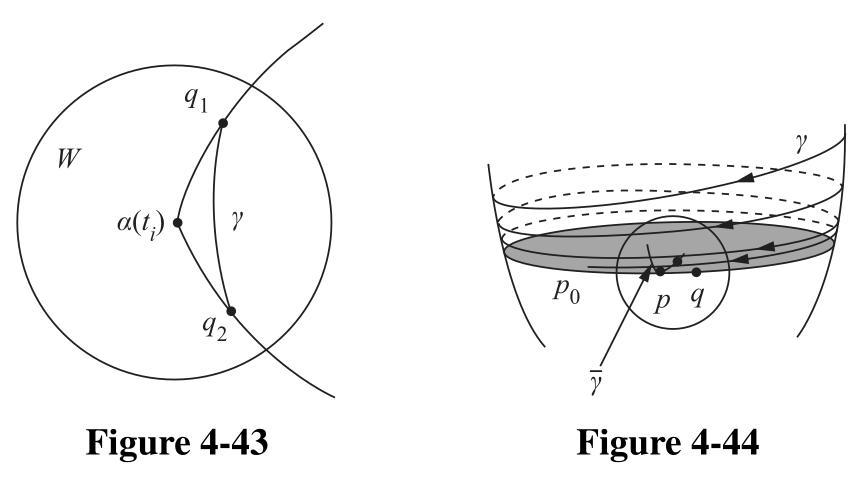
\includegraphics[max width=0.7\textwidth]{images/bo_d4b9jf3ef24c73e0334g_318_352_776_860_484_0.jpg}
\end{center}
\hspace*{3em} 

关于命题1的一个自然问题是，连接 \(W\) 中两点 \({q}_{1},{q}_{2}\) 的长度小于 \(\delta\) 的测地线是否包含在 \(W\) 中.如果对于 \(W\) 中的每对点都成立，我们就说 \(W\) 是凸的.

我们说连接两点的参数化测地线是极小的，如果它的长度小于或等于连接这两点的任何其他参数化分段正则曲线的长度.

当 \(W\) 是凸的时，根据第 4-6 节的命题 4(也参见注记 3)，连接 \({q}_{1} \in  W\) 和 \({q}_{2} \in  W\) 的测地线 \(\gamma\) 是极小的.因此，在这种情况下，我们可以说 \(W\) 中的任意两点由 \(W\) 中的唯一极小测地线连接.然而，通常情况下， \(W\) 不是凸的.

我们现在将证明 \(W\) 可以被选择为凸的.证明的关键在于以下命题，它本身也很有趣.像往常一样，我们用 \({B}_{r}\left( p\right)\) 表示由半径为 \(r\) 、中心为 \(p\) 的测地圆 \({S}_{r}\left( p\right)\) 所围区域的内部.

命题 3. 对于每个点 \(\mathrm{p} \in  S\) ，存在一个正数 \(\epsilon\) ，它具有以下性质:如果一条测地线 \(\gamma \left( \mathrm{t}\right)\) 在 \(\gamma \left( 0\right)\) 处与测地圆 \({S}_{\mathrm{r}}\left( \mathrm{p}\right) ,\mathrm{r} < \epsilon ,\) 相切，那么，当 \(\mathrm{t} \neq  0\) 很小时， \(\gamma \left( t\right)\) 位于 \({\mathrm{B}}_{\mathrm{r}}\left( \mathrm{p}\right)\) 的外部(图 4-45).

\begin{center}
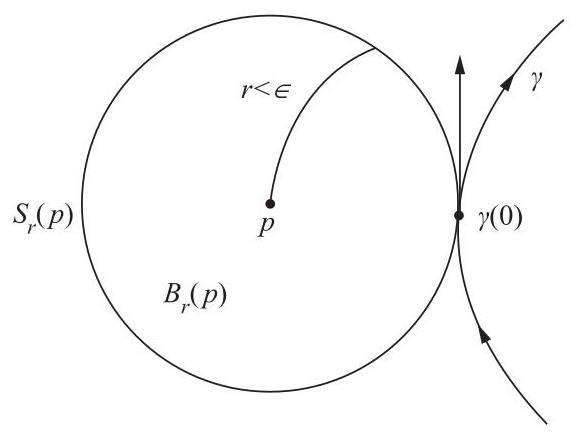
\includegraphics[max width=0.5\textwidth]{images/bo_d4b9jf3ef24c73e0334g_319_181_190_576_439_0.jpg}
\end{center}
\hspace*{3em} 

图 4-45

证明.令 \(W\) 为命题 1 所给的 \(p\) 的邻域.对于每对 \(\left( {q,v}\right) ,q \in  W,v \in  {T}_{q}\left( S\right) ,\left| v\right|  = 1\) ，考虑测地线 \(\gamma \left( {t,q,v}\right)\) ，并为固定的 \(\left( {q,v}\right)\) (图 4-46)设置:

\[
{\exp }_{p}^{-1}\gamma \left( {t,q,v}\right)  = u\left( t\right) ,
\]

\[
F\left( {t,q,v}\right)  = {\left| u\left( t\right) \right| }^{2} = F\left( t\right) .
\]

因此，对于固定的 \(\left( {q,v}\right) ,F\left( t\right)\) ，它是点 \(\gamma \left( {t,q,v}\right)\) 到 \(p\) 的距离的平方.显然， \(F\left( {t,q,v}\right)\) 是可微的.注意到 \(F\left( {t,p,v}\right)  = {\left| vt\right| }^{2}\) .

现在用 \({\mathfrak{U}}^{1}\) 表示集合

\[
{\mathfrak{U}}^{1} = \left\{  {\left( {q,v}\right) ;q \in  W,v \in  {T}_{q}\left( S\right) ,\left| v\right|  = 1}\right\}  ,
\]

并定义函数 \(Q : {\mathfrak{U}}^{1} \rightarrow  R\) 为

\[
Q\left( {q,v}\right)  = {\left. \frac{{\partial }^{2}F}{\partial {t}^{2}}\right| }_{t = 0}.
\]

\begin{center}
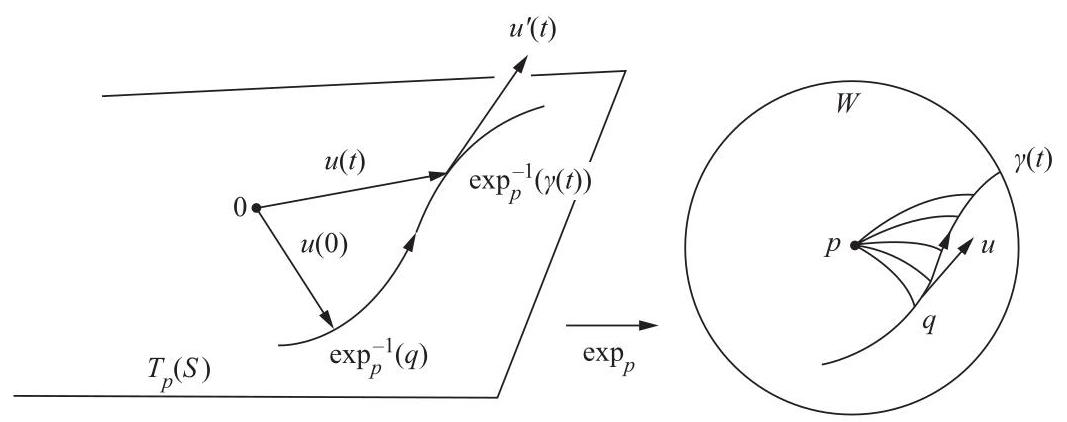
\includegraphics[max width=0.9\textwidth]{images/bo_d4b9jf3ef24c73e0334g_319_236_1618_1067_422_0.jpg}
\end{center}
\hspace*{3em} 

图 4-46

由于 \(F\) 可微， \(Q\) 连续.此外，由于

\[
\frac{\partial F}{\partial t} = 2\left\langle  {u\left( t\right) ,{u}^{\prime }\left( t\right) }\right\rangle  ,
\]

\[
\frac{{\partial }^{2}F}{\partial {t}^{2}} = 2\left\langle  {u\left( t\right) ,{u}^{\prime \prime }\left( t\right) }\right\rangle   + 2\left\langle  {{u}^{\prime }\left( t\right) ,{u}^{\prime }\left( t\right) }\right\rangle  ,
\]

在 \(\left( {p,v}\right)\) 处

\[
{u}^{\prime }\left( t\right)  = v,\;{u}^{\prime \prime }\left( t\right)  = 0,
\]

我们得到

\[
Q\left( {p,v}\right)  = 2{\left| v\right| }^{2} = 2 > 0\;\text{ for all }v \in  {T}_{p}\left( S\right) ,\left| v\right|  = 1.
\]

因此，根据连续性，存在一个邻域 \(V \subset  W\) 使得对于所有 \(q \in  V\) 和 \(v \in  {T}_{q}\left( S\right)\) 且 \(\left| v\right|  = 1\) 的情况，都有 \(Q\left( {q,v}\right)  > 0\) .令 \(\epsilon  > 0\) 使得 \({B}_{\epsilon }\left( p\right)  \subset  V\) .我们声称这个 \(\epsilon\) 满足命题的陈述.

事实上，令 \(r < \epsilon\) ，并令 \(\gamma \left( {t,q,v}\right)\) 是在 \(\gamma \left( 0\right)  = q\) 处切于 \({S}_{r}\left( p\right)\) 的测地线.通过在 \(p\) 周围引入测地极坐标，我们看到 \(\left\langle  {u\left( 0\right) ,{u}^{\prime }\left( 0\right) }\right\rangle   = 0\) (见图 4-47).因此， \(\partial F/\partial t\left( 0\right)  = 0\) .由于 \(F\left( {0,q,v}\right)  = {r}^{2}\) 且 \(\left( {{\partial }^{2}F/\partial {t}^{2}}\right) \left( 0\right)  > 0\) ，我们得到对于小的 \(t \neq  0\) ，有 \(F\left( t\right)  > {r}^{2}\) ；因此， \(\gamma \left( t\right)\) 在 \({B}_{r}\left( p\right)\) 的外部.Q.E.D.

\begin{center}
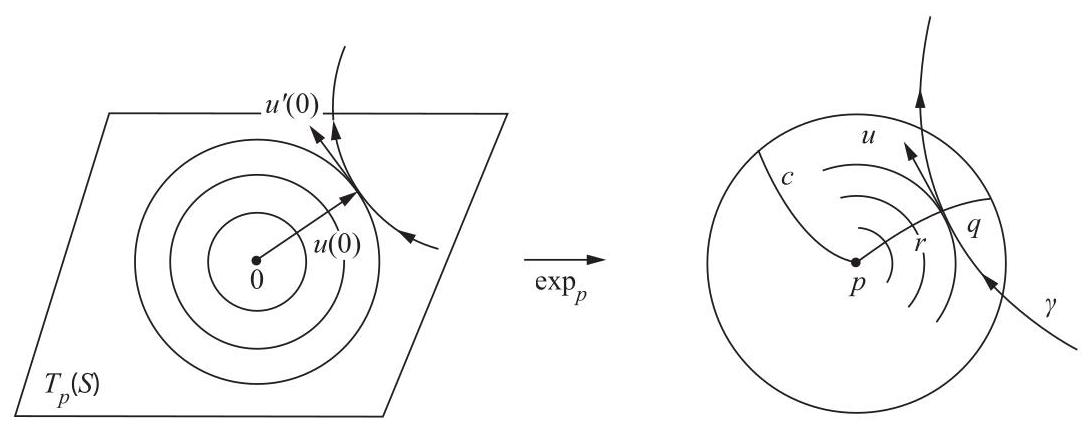
\includegraphics[max width=0.9\textwidth]{images/bo_d4b9jf3ef24c73e0334g_320_238_1172_1092_428_0.jpg}
\end{center}
\hspace*{3em} 

图 4-47

我们现在可以证明

命题 4(凸邻域的存在性).对于每个点 \(\mathrm{p} \in  S\) ，存在一个数 \(\mathrm{c} > 0\) 使得 \({\mathrm{B}}_{\mathrm{c}}\left( \mathrm{p}\right)\) 是凸的；也就是说， \({\mathrm{B}}_{\mathrm{c}}\left( \mathrm{p}\right)\) 中的任意两点都可以通过 \({\mathrm{B}}_{\mathrm{c}}\left( \mathrm{p}\right)\) 中的一条唯一的最小测地线连接.

证明.令 \(\epsilon\) 如命题 3 所示.选择命题 1 中的 \(\delta\) 和 \(W\) 使得 \(\delta  < \epsilon /2\) .选择 \(c < \delta\) 和 使得 \({B}_{c}\left( p\right)  \subset  W\) .我们将证明 \({B}_{c}\left( p\right)\) 是凸的.

令 \({q}_{1},{q}_{2} \in  {B}_{c}\left( p\right)\) ，并令 \(\gamma  : I \rightarrow  S\) 是连接 \({q}_{1}\) 到 \({q}_{2}.\gamma \left( I\right)\) 的长度小于 \(\delta  < \epsilon /2\) 的测地线.显然，它包含在 \({B}_{\epsilon }\left( p\right)\) 中，我们想证明 \(\gamma \left( I\right)\) 包含在 \({B}_{c}\left( p\right)\) 中.假设相反.那么存在一个点 \(m \in  {B}_{\epsilon }\left( p\right)\) ，其中 \(\gamma \left( I\right)\) 到 \(p\) 的最大距离 \(r\) 被达到(图 4-48).在 \(m\) 的邻域中， \(\gamma \left( I\right)\) 的点将在 \({B}_{r}\left( p\right)\) 中.但这与命题 3 矛盾.证毕.

\begin{center}
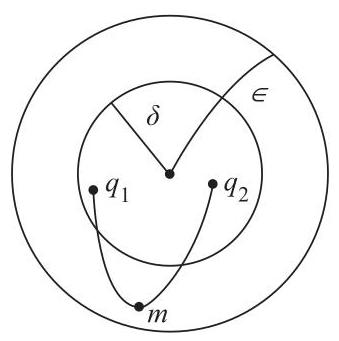
\includegraphics[max width=0.3\textwidth]{images/bo_d4b9jf3ef24c73e0334g_321_181_547_339_341_0.jpg}
\end{center}
\hspace*{3em} 

图 4-48

\exerciseline

*1. 设 \(y\) 和 \(w\) 是开集 \(U \subset  S\) 上的可微向量场.设 \(p \in  S\) 且设 \(\alpha  : I \rightarrow  U\) 是一条曲线，使得 \(\alpha \left( 0\right)  = p,{\alpha }^{\prime }\left( 0\right)  = y\) .令 \({P}_{\alpha ,t} : {T}_{\alpha \left( 0\right) }\left( S\right)  \rightarrow  {T}_{\alpha \left( t\right) }\left( S\right)\) 表示沿 \(\alpha\) 从 \(\alpha \left( 0\right)\) 到 \(\alpha \left( t\right) ,t \in  I\) 的平行移动.证明:

\[
\left( {{D}_{y}w}\right) \left( p\right)  = {\left. \frac{d}{dt}\left( {P}_{\alpha ,t}^{-1}\left( w\left( \alpha \left( t\right) \right) \right) \right) \right| }_{t = 0},
\]

其中第二项是曲线 \({P}_{\alpha ,t}^{-1}\left( {w\left( {\alpha \left( t\right) }\right) }\right)\) 在 \({T}_{p}\left( S\right)\) 中 \(t = 0\) 处的速度向量.(因此，协变导数的概念可以从平行移动的概念导出.)

2. a. 证明协变导数具有以下性质.设 \(v,w\) 和 \(y\) 是 \(U \subset  S,f : U \rightarrow  R\) 中的可微向量场， \(U \subset  S,f : U \rightarrow  R\) 是 \(S,y\left( f\right)\) 中的可微函数， \(f\) 是 \(y\) 方向上的 \(f\) 的导数(参见习题 7，第 3-4 节)， \(\lambda ,\mu\) 是实数.则

1. \({D}_{y}\left( {{\lambda v} + {\mu w}}\right)  = \lambda {D}_{y}\left( v\right)  + \mu {D}_{\gamma }\left( w\right)\) ;

\[
{D}_{{\lambda y} + {\mu v}}\left( w\right)  = \lambda {D}_{y}\left( w\right)  + \mu {D}_{v}\left( w\right) .
\]

2. \({D}_{y}\left( {fv}\right)  = y\left( f\right) v + f{D}_{y}\left( v\right) ;{D}_{fy}\left( v\right)  = f{D}_{y}\left( v\right)\) .

3. \(y\left( {\langle v,w\rangle }\right)  = \left\langle  {{D}_{y}v,w}\right\rangle   + \left\langle  {v,{D}_{y}w}\right\rangle\) .

4. \({D}_{{\mathbf{x}}_{v}}{\mathbf{x}}_{u} = {D}_{{\mathbf{x}}_{u}}{\mathbf{x}}_{v}\) ，其中 \(\mathbf{x}\left( {u,v}\right)\) 是 \(S\) 的参数化.

*b. 证明性质 3 等价于连接两点 \(p,q \in  S\) 的分段正则参数化曲线 \(\alpha  : I \rightarrow  S\) 上的平行移动是 \({T}_{p}\left( S\right)\) 和 \({T}_{q}\left( S\right)\) 之间的等距变换.证明性质 4 等价于克里斯托费尔符号下指标的对称性.

*c. 设 \(\mathfrak{U}\left( U\right)\) 是 \(U \subset  S\) 中(可微)向量场的空间，设 \(D : \mathfrak{U} \times  \mathfrak{U} \rightarrow  \mathfrak{U}\) (其中我们记 \(D\left( {y,v}\right)  = {D}_{y}\left( v\right)\) )是一个满足性质 1-4 的映射.验证 \({D}_{y}\left( v\right)\) 与文本中的协变导数一致.(通常，满足性质 1 和 2 的 \(D\) 称为 \(U\) 中的联络.本题的目的是证明，在具有给定标积的曲面上，存在一个唯一的具有附加性质 3 和 4 的联络.)

*3. 设 \(\alpha  : I = \left\lbrack  {0,l}\right\rbrack   \rightarrow  S\) 是一条简单、参数化、正则曲线.考虑沿 \(\alpha\) 的单位向量场 \(v\left( t\right)\) ，其中 \(\left\langle  {{\alpha }^{\prime }\left( t\right) ,v\left( t\right) }\right\rangle   = 0\) ，以及一个映射 x: \(R \times  I \rightarrow  S\) ，由下式给出:

\[
\mathbf{x}\left( {s,t}\right)  = {\exp }_{\alpha \left( t\right) }\left( {{sv}\left( t\right) }\right) ,\;s \in  R,t \in  I.
\]

a. 证明 \(\mathbf{x}\) 在 \(R \times  I\) 中 \(I\) 的邻域内是可微的，并且 \(d\mathbf{x}\) 在 \(\left( {0,t}\right) ,t \in  I\) 中是非奇异的.

b. 证明存在 \(\epsilon  > 0\) 使得 \(\mathbf{x}\) 在矩形 \(t \in  I,\left| s\right|  < \epsilon\) 中是一一对应的.

c. 证明在开集 \(t \in  \left( {0,l}\right) ,\left| s\right|  < \epsilon ,\mathbf{x}\) 中是 \(S\) 的一个参数化，其坐标邻域包含 \(\alpha \left( \left( {0,l}\right) \right)\) .由此得到的坐标称为基 \(\alpha\) 的测地坐标(或费米坐标).证明在此类系统中 \(F = 0,E = 1\) .此外，如果 \(\alpha\) 是由弧长参数化的测地线，则 \(G\left( {0,t}\right)  =\) 1 且 \({G}_{s}\left( {0,t}\right)  = 0\) .

d. 建立高斯引理的以下类似物(第 4-6 节命题 3 后的备注 1).设 \(\alpha  : I \rightarrow  S\) 为正则参数化曲线，设 \({\gamma }_{t}\left( s\right) ,t \in  I\) 为由弧长 \(s\) 参数化并由以下方式给出的测地线族: \({\gamma }_{t}\left( 0\right)  = \alpha \left( t\right) ,\left\{  {{\gamma }_{t}^{\prime }\left( 0\right) ,{\alpha }^{\prime }\left( t\right) }\right\}\) 为正交基.那么，对于固定的 \(\bar{s}\) ，足够小，曲线 \(t \rightarrow  {\gamma }_{t}\left( \bar{s}\right) ,t \in  I\) 与所有 \({\gamma }_{t}\) 正交相交(此类曲线称为测地线平行线).

4. 曲线 \(\alpha  : \left\lbrack  {a,b}\right\rbrack   \rightarrow  S\) 的能量 \(E\) 定义为

\[
E\left( \alpha \right)  = {\int }_{a}^{b}{\left| {\alpha }^{\prime }\left( t\right) \right| }^{2}{dt}
\]

*a. 证明 \({\left( I\left( \alpha \right) \right) }^{2} \leq  \left( {b - a}\right) E\left( \alpha \right)\) 且当且仅当 \(t\) 与弧长成比例时等式成立.

b. 从 a 部分得出结论，如果 \(\gamma  : \left\lbrack  {a,b}\right\rbrack   \rightarrow  S\) 是具有 \(\gamma \left( a\right)  = p,\gamma \left( b\right)  = q\) 的最小测地线，那么对于连接 \(p\) 到 \(q\) 的任何曲线 \(\alpha  : \left\lbrack  {a,b}\right\rbrack   \rightarrow  S\) ，我们有 \(E\left( \gamma \right)  \leq  E\left( \alpha \right)\) 且当且仅当 \(\alpha\) 是最小测地线时等式成立.

5. 设 \(\gamma  : \left\lbrack  {0,l}\right\rbrack   \rightarrow  S\) 为由弧长参数化的简单测地线，并设 \(u\) 和 \(v\) 为 \(\gamma \left( \left\lbrack  {0,l}\right\rbrack  \right)\) 邻域中的费米坐标，其中 \(\gamma \left( \left\lbrack  {0,l}\right\rbrack  \right)\) 由 \(u = 0\) 给出(参见练习 3).设 \(u = \gamma \left( {v,t}\right)\) 为依赖于参数 \(t, - \epsilon  < t < \epsilon\) 的曲线族，使得 \(\gamma\) 可微且

\[
\gamma \left( {0,t}\right)  = \gamma \left( 0\right)  = p,\;\gamma \left( {l,t}\right)  = \gamma \left( l\right)  = q,\;\gamma \left( {v,0}\right)  = \gamma \left( v\right)  \equiv  0.
\]

这样的族称为 \(\gamma\) 的变分，保持端点 \(p\) 和 \(q\) 固定.设 \(E\left( t\right)\) 为曲线 \(\gamma \left( {v,t}\right)\) 的能量(参见练习 4)；即，

\[
E\left( t\right)  = {\int }_{0}^{l}{\left( \frac{\partial \gamma }{\partial v}\left( v,t\right) \right) }^{2}{dv}.
\]

*a. 证明

\[
{E}^{\prime }\left( 0\right)  = 0
\]

\[
\frac{1}{2}{E}^{\prime \prime }\left( 0\right)  = {\int }_{0}^{l}\left\{  {{\left( \frac{d\eta }{dv}\right) }^{2} - K{\eta }^{2}}\right\}  {dv},
\]

其中 \(\eta \left( v\right)  = \partial \gamma /{\left. \partial t\right| }_{t = 0},\;K = K\left( v\right)\) 是 \(\gamma\) 上的高斯曲率，表示对 \(t\) 的导数(上述公式分别称为 \(\gamma\) 的能量的第一次和第二次变分；更完整的处理这些公式，包括 \(\gamma\) 不简单的情况，将在第 5-4 节给出).

b. 从 a 部分得出结论，如果 \(K \leq  0\) ，则任何简单的测地线 \(\gamma  : \left\lbrack  {0,l}\right\rbrack   \rightarrow  S\) 相对于足够接近 \(\gamma\) 且连接 \(\gamma \left( 0\right)\) 和 \(\gamma \left( l\right)\) 的曲线都是极小的.

6. 令 \(S\) 为圆锥 \(z = k\sqrt{{x}^{2} + {y}^{2}},k > 0,\left( {x,y}\right)  \neq  \left( {0,0}\right)\) ，令 \(V \subset  {R}^{2}\) 为 \({R}^{2}\) 的开集，在极坐标中由 \(0 < \rho  < \infty ,0 < \; \theta  < {2\pi n}\sin \beta\) 给出，其中 cotan \(\beta  = k\) 且 \(n\) 是满足 \({2\pi n}\sin \beta  < {2\pi }\) 的最大整数(参见第 4-2 节的示例 3).令 \(\varphi  : V \rightarrow  S\) 为映射

\[
\varphi \left( {\rho ,\theta }\right)  = \left( {\rho \sin \beta \cos \left( \frac{\theta }{\sin \beta }\right) ,\rho \sin \beta \sin \left( \frac{\theta }{\sin \beta }\right) ,\rho \cos \beta }\right) .
\]

a. 证明 \(\varphi\) 是局部等距变换.

\begin{center}
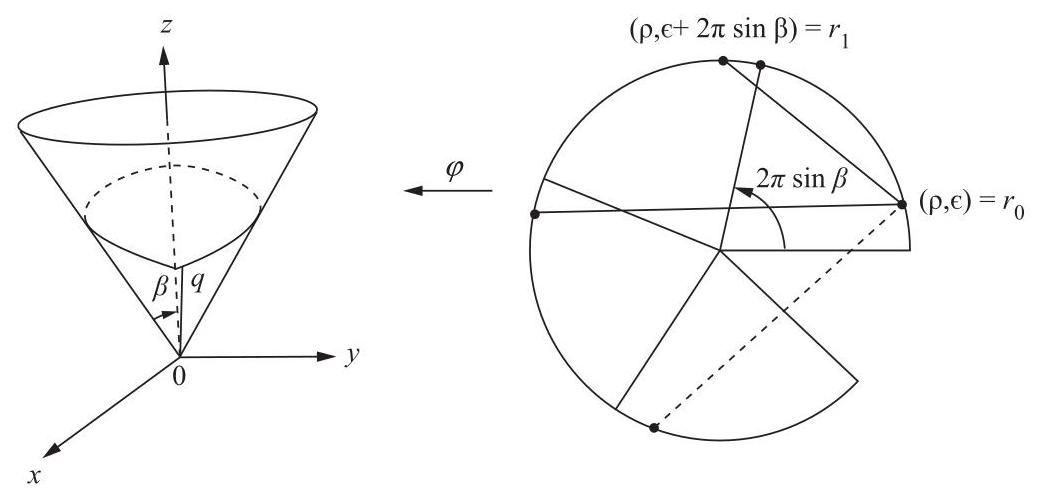
\includegraphics[max width=0.9\textwidth]{images/bo_d4b9jf3ef24c73e0334g_324_258_195_1039_495_0.jpg}
\end{center}
\hspace*{3em} 

图 4-49

b. 令 \(q \in  S\) .假设 \(\beta  < \pi /6\) 且令 \(k\) 是满足 \({2\pi k}\sin \beta  < \pi\) 的最大整数.证明存在至少 \(k\) 条从 \(q\) 出发并返回 \(q\) 的测地线.证明这些测地线在 \(q\) 处断开，因此它们都不是闭合测地线(图 4-49).

*c. 在 \(\mathrm{b}\) 条件下，证明存在恰好 \(k\) 条这样的测地线.

7. 令 \(\alpha  : I - {R}^{3}\) 为参数化的正则曲线.对于每个 \(t \in  I\) ，令 \(P\left( t\right)  \subset \; {R}^{3}\) 为通过 \(\alpha \left( t\right)\) 且包含 \({\alpha }^{\prime }\left( t\right)\) 的平面.当 \(P\left( t\right)\) 的单位法向量 \(N\left( t\right)\) 是 \(t\) 和 \({N}^{\prime }\left( t\right)  \neq  0,t \in  I\) 的可微函数时，我们称映射 \(t \rightarrow  \{ \alpha \left( t\right) ,N\left( t\right) \}\) 是切平面族的可微族.给定这样的族，我们通过(参见第 2-3 节的定义 2)确定一个参数化曲面

\[
\mathbf{x}\left( {t,v}\right)  = \alpha \left( t\right)  + v\frac{N\left( t\right)  \land  {N}^{\prime }\left( t\right) }{\left| {N}^{\prime }\left( t\right) \right| }.
\]

参数化曲面 \(\mathbf{x}\) 称为族 \(\{ \alpha \left( t\right) ,N\left( t\right) \}\) 的包络(参见第 3-5 节的示例 4).

a. 令 \(S\) 为一个定向曲面，令 \(\gamma  : I \rightarrow  S\) 为一条由弧长参数化的测地线，其端点为 \(k\left( s\right)  \neq  0\) 和 \(\tau \left( s\right)  \neq  0,s \in  I\) .令 \(N\left( s\right)\) 为 \(S\) 在 \(\gamma\) 处的单位法向量.证明:切平面族 \(\{ \gamma \left( s\right) ,N\left( s\right) \}\) 的包络在 \(\gamma\) 的邻域内是正则的，具有高斯曲率 \(K \equiv  0\) ，并且在 \(\gamma\) 处与 \(S\) 相切.(因此，我们得到了一个局部等距于平面且包含 \(\gamma\) 作为测地线的曲面.)

b. 令 \(\alpha  : I \rightarrow  {R}^{3}\) 为一条由弧长参数化的曲线，其端点为 \(k\left( s\right)  \neq  0\) 和 \(\tau \left( s\right)  \neq  0,s \in  I\) ，令 \(\{ \alpha \left( s\right) ,n\left( s\right) \}\) 为其法平面族.证明:该族包络在 \(\alpha\) 的邻域内是正则的，具有高斯曲率 \(K = 0\) ，并且包含 \(\alpha\) 作为测地线.(因此，每条曲线都是其法平面族包络中的测地线；由于该包络局部等距于平面，这证明了法平面名称的合理性.)

8. (小测地线三角形的自由移动性.)令 \(S\) 为一个高斯曲率为常数的曲面.选择点 \({p}_{1},{p}_{1}^{\prime } \in  S\) ，并令 \(V,{V}^{\prime }\) 分别为 \({p}_{1},{p}_{1}^{\prime }\) 的凸邻域.在 \(v\) 中选择测地线三角形 \({p}_{1},{p}_{2},{p}_{3}\) (测地线意味着边 \(\widehat{{p}_{1}}{p}_{2},\widehat{{p}_{2}}{p}_{3},\widehat{{p}_{3}}{p}_{1}\) 是测地线弧)，在 \(V\) 中选择测地线三角形 \({p}_{1},{p}_{2},{p}_{3}\) ，在 \({V}^{\prime }\) 中选择测地线三角形 \({p}_{1}^{\prime },{p}_{2}^{\prime },{p}_{3}^{\prime }\) ，使得

\[
l\left( {{p}_{1},{p}_{2}}\right)  = l\left( {{p}_{1}^{\prime },{p}_{2}^{\prime }}\right) ,
\]

\[
l\left( {{p}_{2},{p}_{3}}\right)  = l\left( {{p}_{2}^{\prime },{p}_{3}^{\prime }}\right) ,
\]

\[
l\left( {{p}_{3},{p}_{1}}\right)  = l\left( {{p}_{3}^{\prime },{p}_{1}^{\prime }}\right)
\]

(此处 \(l\) 表示测地线弧的长度).证明存在一个等距映射 \(\theta  : V \rightarrow  {V}^{\prime }\) ，将第一个三角形映射到第二个三角形.(这是常曲率曲面的局部版本，对应于平面几何中“任意两个对应边相等的三角形都全等”的定理.)

附录 曲线和曲面局部理论的基本定理证明

在本附录中，我们将展示如何从微分方程的定理中得到曲线和曲面的存在唯一性基本定理(第 1-5 节和 4-2 节).

曲线局部理论基本定理证明(参见第 1-5 节的陈述).出发点是观察到弗雷内方程

\[
\frac{dt}{ds} = {kn}
\]

\[
\frac{dn}{ds} =  - {kt} - {\tau b} \tag{1}
\]

\[
\frac{db}{ds} = {\tau n}
\]

可以看作是关于 \(I \times  {R}^{9}\) 的一个微分系统，

\[
\left. \begin{array}{l} \frac{d{\xi }_{1}}{ds} = {f}_{1}\left( {s,{\xi }_{1},\ldots ,{\xi }_{9}}\right) \\  \vdots \\  \frac{d{\xi }_{9}}{ds} = {f}_{9}\left( {s,{\xi }_{1},\ldots ,{\xi }_{9}}\right)  \end{array}\right\}  ,\;s \in  I, \tag{1a}
\]

其中 \(\left( {{\xi }_{1},{\xi }_{2},{\xi }_{3}}\right)  = t,\left( {{\xi }_{4},{\xi }_{5},{\xi }_{6}}\right)  = n,\left( {{\xi }_{7},{\xi }_{8},{\xi }_{9}}\right)  = b\) ，以及 \({f}_{i},i = 1,\ldots ,9\) ，是坐标 \({\xi }_{i}\) 的线性函数(系数依赖于 \(s\) ).

一般而言，类型为 (1a) 的微分系统不能与一个“稳态”向量场相关联(如第 3-4 节所示).无论如何，存在唯一性定理以如下形式成立:

给定初始条件 \({S}_{0} \in  \mathrm{I},{\left( {\xi }_{1}\right) }_{0},\ldots ,{\left( {\xi }_{9}\right) }_{0}\) ，存在包含 \({S}_{0}\) 的开区间 \(\mathrm{J} \subset  \mathrm{I}\) 和唯一的微分映射 \(\alpha  : \mathrm{J} \rightarrow  {\mathbb{R}}^{9}\) ，其中

\[
\alpha \left( {S}_{0}\right)  = \left( {{\left( {\xi }_{1}\right) }_{0},\ldots ,{\left( {\xi }_{9}\right) }_{0}}\right) \;\text{ and }\;{\alpha }^{\prime }\left( S\right)  = \left( {{\mathrm{f}}_{1},\ldots ,{\mathrm{f}}_{9}}\right) ,
\]

其中每个 \({\mathrm{f}}_{\mathrm{i}},\mathrm{i} = 1,\ldots ,9\) 都在 \(\left( {S,\alpha \left( S\right) }\right)  \in  \mathrm{J} \times  {\mathbb{R}}^{9}\) 中计算.此外，如果系统是线性的， \(\mathrm{J} = \mathrm{I}\) (参见 S. Lang, Analysis I, Addison-Wesley, Reading, Mass., 1968, pp. 383-386).

由此可知，给定 \({R}^{3}\) 中的一个标准正交、定向的 삼면체 \(\left\{  {{t}_{0},{n}_{0},{b}_{0}}\right\}\) 和一个值 \({s}_{0} \in  I\) ，存在一个 삼면体族 \(\{ t\left( s\right) ,n\left( s\right) ,b\left( s\right) \} ,s \in  I\) ，其中 \(t\left( {s}_{0}\right)  = {t}_{0},n\left( {s}_{0}\right)  = {n}_{0},b\left( {s}_{0}\right)  = {b}_{0}\) .

我们首先证明所获得的族 \(\{ t\left( s\right) ,n\left( s\right) ,b\left( s\right) \}\) 对于每个 \(s \in  I\) 都保持标准正交.事实上，通过使用系统 (1) 来表示六个量的 \(s\) 导数

\[
\langle t,n\rangle ,\;\langle t,b\rangle ,\;\langle n,b\rangle ,\;\langle t,t\rangle ,\;\langle n,n\rangle ,\;\langle b,b\rangle
\]

作为这些量本身的函数，我们得到微分方程组

\[
\frac{d}{ds}\langle t,n\rangle  = k\langle n,n\rangle  - k\langle t,t\rangle  - \tau \langle t,b\rangle ,
\]

\[
\frac{d}{ds}\langle t,b\rangle  = k\langle n,b\rangle  + \tau \langle t,n\rangle ,
\]

\[
\frac{d}{ds}\langle n,b\rangle  =  - k\langle t,b\rangle  - \tau \langle b,b\rangle  + \tau \langle n,n\rangle ,
\]

\[
\frac{d}{ds}\langle t,t\rangle  = {2k}\langle t,n\rangle
\]

\[
\frac{d}{ds}\langle n,n\rangle  =  - {2k}\langle n,t\rangle  - {2\tau }\langle n,b\rangle ,
\]

\[
\frac{d}{ds}\langle b,b\rangle  = {2\tau }\langle b,n\rangle
\]

很容易检查出

\[
\langle t,n\rangle  \equiv  0,\;\langle t,b\rangle  \equiv  0,\;\langle n,b\rangle  \equiv  0,
\]

\[
{t}^{2} \equiv  1,{n}^{2} \equiv  1,{b}^{2} \equiv  1,
\]

是上述系统在初始条件 0,0,0,1,1,1 下的解.根据唯一性，族 \(\{ t\left( s\right) ,n\left( s\right) ,b\left( s\right) \}\) 对于每个 \(s \in  I\) 都标准正交，正如我们所声称的.

从族 \(\{ t\left( s\right) ,n\left( s\right) ,b\left( s\right) \}\) 可以通过设置得到一条曲线

\[
\alpha \left( s\right)  = \int t\left( s\right) {ds},\;s \in  I,
\]

其中向量的积分是指通过对每个分量进行积分得到的向量函数.显然 \({\alpha }^{\prime }\left( s\right)  = t\left( s\right)\) 并且 \({\alpha }^{\prime \prime }\left( s\right)  = {kn}\) .因此， \(k\left( s\right)\) 是 \(\alpha\) 在 \(s\) 处的曲率.此外，由于

\[
{\alpha }^{\prime \prime \prime }\left( s\right)  = {k}^{\prime }n + k{n}^{\prime } = {k}^{\prime }n - {k}^{2}t - {k\tau b},
\]

\(\alpha\) 的挠率由下式给出 (参见练习 12, 第 1-5 节)

\[
- \frac{\left\langle  \alpha  \land  {\alpha }^{\prime \prime },{\alpha }^{\prime \prime \prime }\right\rangle  }{{k}^{2}} =  - \frac{\left\langle  t \land  kn,\left( -{k}^{2}t + {k}^{\prime }n - k\tau b\right) \right\rangle  }{{k}^{2}} = \tau ;
\]

\(\alpha\) 因此是所需的曲线.

我们仍需证明 \(\alpha\) 在平移和旋转 \({R}^{3}\) 下是唯一的.设 \(\overline{\alpha } : I \rightarrow  {R}^{3}\) 是另一条曲线，具有 \(\bar{k}\left( s\right)  = k\left( s\right)\) 和 \(\overline{\tau }\left( s\right)  = \tau \left( s\right) ,s \in  I\) ，设 \(\left\{  {{\bar{t}}_{0},{\bar{n}}_{0},{\bar{b}}_{0}}\right\}\) 是 \(\overline{\alpha }\) 在 \({s}_{0}\) 处的弗雷内三面体.显然，通过平移 \(A\) 和旋转 \(\rho\) ，可以使三面体 \(\left\{  {{\bar{t}}_{0},{\bar{n}}_{0},{\bar{b}}_{0}}\right\}\) 与三面体 \(\left\{  {{t}_{0},{n}_{0},{b}_{0}}\right\}\) 重合(两个三面体都是正的).通过应用上述微分方程定理的唯一性部分，我们得到所需的结果.证毕.

局部曲面理论基本定理的证明(参见第 4-3 节的陈述).证明思路与上述相同；也就是说，我们寻找一个三面体族 \(\left\{  {{\mathbf{x}}_{u},{\mathbf{x}}_{v},N}\right\}\) ，它依赖于 \(u\) 和 \(v\) ，并满足以下方程组

\[
{\mathbf{x}}_{uu} = {\mathbf{\Gamma }}_{11}^{1}{\mathbf{x}}_{u} + {\mathbf{\Gamma }}_{11}^{2}{\mathbf{x}}_{v} + {eN}
\]

\[
{\mathbf{x}}_{uv} = {\mathbf{\Gamma }}_{12}^{1}{\mathbf{x}}_{u} + {\mathbf{\Gamma }}_{12}^{2}{\mathbf{x}}_{v} + {fN} = {\mathbf{x}}_{vu}
\]

\[
{\mathbf{x}}_{vv} = {\mathbf{\Gamma }}_{22}^{1}{\mathbf{x}}_{u} + {\mathbf{\Gamma }}_{22}^{2}{\mathbf{x}}_{v} + {gN} \tag{2}
\]

\[
{N}_{u} = {a}_{11}{\mathbf{x}}_{u} + {a}_{21}{\mathbf{x}}_{v},
\]

\[
{N}_{v} = {a}_{12}^{1}{\mathbf{x}}_{u} + {a}_{22}{\mathbf{x}}_{v},
\]

其中系数 \({\mathbf{\Gamma }}_{ij}^{k},{a}_{ij},i,j,k = 1,2\) ，是从 \(E,F,G,e,f,g\) 得到的，就好像它在曲面上一样.

上述方程定义了一个关于 \(V \times  {R}^{9},\) 的偏微分方程组

\[
{\left( {\xi }_{1}\right) }_{u} = {f}_{1}\left( {u,v,{\xi }_{1},\ldots ,{\xi }_{9}}\right) ,
\]

(2a)

\[
{\left( {\xi }_{9}\right) }_{v} = {f}_{15}\left( {u,v,{\xi }_{1},\ldots ,{\xi }_{9}}\right) ,
\]

其中 \(\xi  = \left( {{\xi }_{1},{\xi }_{2},{\xi }_{3}}\right)  = {\mathbf{x}}_{u},\eta  = \left( {{\xi }_{4},{\xi }_{5},{\xi }_{6}}\right)  = {\mathbf{x}}_{v},\zeta  = \left( {{\xi }_{7},{\xi }_{8},{\xi }_{9}}\right)  = N\) 和 \({f}_{i} = 1,\ldots ,{15}\) 是坐标 \({\xi }_{j},j = 1,\ldots ,9\) 的线性函数，系数依赖于 \(u\) 和 \(v\) .

与常微分方程的情况不同，(2a)类型的方程组通常是不可积的.对于所讨论的情况，保证局部解的存在性和唯一性的条件是

\[
{\xi }_{uv} = {\xi }_{vu},\;{\eta }_{uv} = {\eta }_{vu},\;{\zeta }_{uv} = {\zeta }_{vu}.
\]

该论断的证明可在 J. Stoker 的《微分几何》中找到，Wiley Interscience，纽约，1969 年，附录 B.

正如我们在第 4-3 节中所见，可积性条件等价于高斯方程和主科达齐方程，根据假设，这些方程是满足的.因此，方程组(2a)是可积的.

设 \(\{ \xi ,\eta ,\zeta \}\) 是在 \(\left( {{u}_{0},{v}_{0}}\right)  \in \; V\) 的邻域中定义的(2a)的一个解，具有初始条件 \(\xi \left( {{u}_{0},{v}_{0}}\right)  = {\xi }_{0},\eta \left( {{u}_{0},{v}_{0}}\right)  = {\eta }_{0},\zeta \left( {{u}_{0},{v}_{0}}\right)  = {\zeta }_{0}\) .显然，可以选择初始条件，使得

\[
{\xi }_{0}^{2} = E\left( {{u}_{0},{v}_{0}}\right)
\]

\[
{\eta }_{0}^{2} = G\left( {{u}_{0},{v}_{0}}\right) ,
\]

\[
\left\langle  {{\xi }_{0},{\eta }_{0}}\right\rangle   = F\left( {{u}_{0},{v}_{0}}\right) , \tag{3}
\]

\[
{\zeta }_{0}^{2} = 1
\]

\[
\left\langle  {{\xi }_{0},{\zeta }_{0}}\right\rangle   = \left\langle  {{\eta }_{0},{\zeta }_{0}}\right\rangle   = 0.
\]

利用给定的解，我们构造一个新的方程组，

\[
{\mathbf{x}}_{u} = \xi \tag{4}
\]

\[
{\mathbf{x}}_{v} = \eta
\]

显然可积，因为 \({\xi }_{v} = {\eta }_{u}\) .令 \(\mathbf{x} : \bar{V} \rightarrow  {R}^{3}\) 为 (4) 的一个解，定义在 \(\left( {{u}_{0},{v}_{0}}\right)\) 的邻域 \(\bar{V}\) 中，且有 \(\mathbf{x}\left( {{u}_{0},{v}_{0}}\right)  = {p}_{0} \in  {R}^{3}\) .我们将证明，通过收缩 \(\bar{V}\) 并必要时交换 \(v\) 和 \(u\) ， \(\mathbf{x}\left( \bar{V}\right)\) 是所需的曲面.

我们首先证明族 \(\{ \xi ,\eta ,\zeta \}\) 是 (2a) 的一个解，并具有以下性质.对于解所定义的每个 \(\left( {u,v}\right)\) ，我们有

\[
{\xi }^{2} = E
\]

\[
{\eta }^{2} = G
\]

\[
\langle \xi ,\eta \rangle  = F \tag{5}
\]

\[
{\zeta }^{2} = 1
\]

\[
\langle \xi ,\zeta \rangle  = \langle \eta ,\zeta \rangle  = 0.
\]

事实上，通过使用 (2) 来表示的偏导数

\[
{\xi }^{2},\;{\eta }^{2},\;{\zeta }^{2},\;\langle \xi ,\eta \rangle ,\;\langle \xi ,\zeta \rangle ,\;\langle \eta ,\zeta \rangle
\]

作为这 6 个量本身的函数，我们得到一个 12 个偏微分方程的系统:

\[
{\left( {\xi }^{2}\right) }_{u} = {B}_{1}\left( {{\xi }^{2},{\eta }^{2},\ldots ,\langle \eta ,\zeta \rangle }\right) ,
\]

\[
{\left( {\xi }^{2}\right) }_{v} = {B}_{2}\left( {{\xi }^{2},{\eta }^{2},\ldots ,\langle \xi ,\zeta \rangle }\right) ,
\]

(6)

\[
{\left( \eta ,\zeta \right) }_{v} = {B}_{12}\left( {{\xi }^{2},{\eta }^{2},\ldots ,\langle \eta ,\zeta \rangle }\right) .
\]

由于 (6) 是从 (2a) 得到的，因此很清楚(并且可以直接验证)(6) 是可积的，并且

\[
{\xi }^{2} = E
\]

\[
{\eta }^{2} = G
\]

\[
\langle \eta ,\xi \rangle  = F,
\]

\[
{\zeta }^{2} = 1
\]

\[
\langle \xi ,\zeta \rangle  = \langle \eta ,\zeta \rangle  = 0
\]

是 (6) 的一个解，具有初始条件 (3).根据唯一性，我们得到我们的结论.

由此可知

\[
{\left| {\mathbf{x}}_{u} \land  {\mathbf{x}}_{v}\right| }^{2} = {\mathbf{x}}_{u}^{2}{\mathbf{x}}_{v}^{2} - {\left\langle  {\mathbf{x}}_{u},{\mathbf{x}}_{v}\right\rangle  }^{2} = {EG} - {F}^{2} > 0.
\]

因此，如果 \(\mathbf{x} : \bar{V} \rightarrow  {R}^{3}\) 由下式给出

\[
\mathbf{x}\left( {uv}\right)  = \left( {x\left( {u,v}\right) ,y\left( {u,v}\right) ,z\left( {u,v}\right) }\right) ,\;\left( {u,v}\right)  \in  \bar{V},
\]

\({\mathbf{x}}_{u} \land  {\mathbf{x}}_{v}\) 的一个分量，例如 \(\partial \left( {x,y}\right) /\partial \left( {u,v}\right)\) ，在 \(\left( {{u}_{0},{v}_{0}}\right)\) 中不为零.因此，我们可以在 \(\left( {{u}_{0},{v}_{0}}\right)\) 的邻域 \(U \subset  \bar{V}\) 中，通过反转 \(\mathbf{x}\) 的前两个分量函数构成的系统，得到一个映射 \(F\left( {x,y}\right)  = \left( {u,v}\right)\) .通过将 \(\mathbf{x}\) 限制在 \(U\) 上，映射 \(\mathbf{x} : U \rightarrow  {R}^{3}\) 是单射的，并且其逆映射 \({\mathbf{x}}^{-1} = F \circ  \pi\) (其中 \(\pi\) 是 \({R}^{3}\) 在 \({xy}\) 平面上的投影)是连续的.因此， \(\mathbf{x} : U \rightarrow  {R}^{3}\) 是一个可微同胚，具有 \({\mathbf{x}}_{u} \land  {\mathbf{x}}_{v} \neq  0\) ；因此， \(\mathbf{x}\left( U\right)  \subset  {R}^{3}\) 是一个正则曲面.

从 (5) 可以直接得出 \(E,F,G\) 是 \(\mathbf{x}\left( U\right)\) 的第一基本形式的系数，并且 \(\zeta\) 是垂直于曲面的单位法向量.必要时交换 \(v\) 和 \(u\) ，我们得到

\[
\zeta  = \frac{{\mathbf{x}}_{u} \land  {\mathbf{x}}_{v}}{\left| {\mathbf{x}}_{u} \land  {\mathbf{x}}_{v}\right| } = N.
\]

由此，通过 (2) 计算出 \(\mathbf{x}\left( {u,v}\right)\) 的第二基本形式的系数，得到

\[
\left\langle  {\zeta ,{\mathbf{x}}_{uu}}\right\rangle   = e,\;\left\langle  {\zeta ,{\mathbf{x}}_{uv}}\right\rangle   = f,\;\left\langle  {\zeta ,{\mathbf{x}}_{vv}}\right\rangle   = g,
\]

这表明这些系数是 \(e,f,g\) ，并完成了证明的第一部分.

剩下要证明的是，如果 \(U\) 是连通的，那么 \(\mathbf{x}\) 在 \({R}^{3}\) 的平移和旋转下是唯一的.为此，设 \(\overline{\mathbf{x}} : U \rightarrow  {R}^{3}\) 是另一个正则曲面，具有 \(\bar{E} = E,\bar{F} = F,\bar{G} = G,\bar{e} = e,\bar{f} = f\) 和 \(\bar{g} = g\) .由于第一和第二基本形式相等，可以通过平移 \(U\) 和旋转 \(\mathbf{x}\) 将三面体

\[
\left\{  {{\overline{\mathbf{x}}}_{u}\left( {{u}_{0},{v}_{0}}\right) ,{\overline{\mathbf{x}}}_{v}\left( {{u}_{0},{v}_{0}}\right) ,\bar{N}\left( {{u}_{0},{v}_{0}}\right) }\right\}
\]

与三面体

\[
\left\{  {{\mathbf{x}}_{u}\left( {{u}_{0},{v}_{0}}\right) ,{\mathbf{x}}_{v}\left( {{u}_{0},{v}_{0}}\right) ,N\left( {{u}_{0},{v}_{0}}\right) }\right\}
\]

通过一个 \(A\) 的平移和一个 \(\rho\) 的旋转.

系统 (1a) 由两个解满足.

\[
\xi  = {\mathbf{x}}_{u},\;\eta  = {\mathbf{x}}_{v},\;\zeta  = N
\]

\[
\xi  = {\overline{\mathbf{x}}}_{u},\;\eta  = {\overline{\mathbf{x}}}_{v},\;\zeta  = \bar{N}.
\]

由于两个解在 \(\left( {{u}_{0},{v}_{0}}\right)\) 处重合，我们根据唯一性得到

\[
{\mathbf{x}}_{u} = {\overline{\mathbf{x}}}_{u},\;{\mathbf{x}}_{v} = {\overline{\mathbf{x}}}_{v},\;N = \bar{N}, \tag{7}
\]

在 \(\left( {{u}_{0},{v}_{0}}\right)\) 的邻域内.另一方面，根据连续性，(7)成立的 \(U\) 的子集是闭集.由于 \(U\) 是连通的，(7)对所有 \(\left( {u,v}\right)  \in  U\) 成立.

从 (7) 的前两个方程以及 \(U\) 是连通的事实，我们得出

\[
\mathbf{x}\left( {u,v}\right)  = \overline{\mathbf{x}}\left( {u,v}\right)  + C,
\]

其中 \(C\) 是一个常向量.由于 \(\mathbf{x}\left( {{u}_{0},{v}_{0}}\right)  = \overline{\mathbf{x}}\left( {{u}_{0},{v}_{0}}\right)\) ，我们得到 \(C = 0\) ，这就完成了定理的证明.Q.E.D.

\section*{5 全微分几何}

\section*{5-1. 引言}

本章的目的是介绍全微分几何.我们已经遇到过全局定理(第 2-7 节中紧致可定向曲面的刻画和第 4-5 节中的高斯-博内定理是一些例子).然而，这些定理或多或少是顺带遇到的，我们的主要任务是为 \({R}^{3}\) 中正则曲面的局部理论奠定基础.现在，这些都已完成，我们可以开始更系统地研究全局性质.

全微分几何处理曲线和曲面的局部性质与全局(通常是拓扑)性质之间的关系.我们试图通过将自己限制在欧几里得空间子集上来最小化拓扑学的要求.只使用了欧几里得空间连通和紧致子集的最基本性质.为完整起见，这些材料在第 5 章的附录中提供了证明.

在使用本章时，读者可以做出多种选择，并考虑到这一点，我们将简要介绍本章各节的内容.在本引言的末尾，将给出各节的依赖关系表.

在第 5-2 节中，我们将证明球是刚性的；也就是说，如果一个连通的、紧致的、正则曲面 \(S \subset  {R}^{3}\) 与一个球等距，那么 \(S\) 是一个球.除了作为第 5-3 节的动机外，本节在本书中不被使用.

在第 5-3 节中，我们将引入完备曲面的概念，作为全局定理的自然背景.我们将证明基本的海夫纳-林诺定理，该定理断言在完备曲面的任意两点之间存在一条极小测地线.

在第 5-4 节中，我们将推导弧长的一阶和二阶变分公式.作为应用，我们将证明邦内定理:具有正且远离零的高斯曲率的完备曲面是紧致的.

在第 5-5 节中，我们将引入测地线 \(\gamma\) 上的雅可比场的重要概念，它衡量 \(\gamma\) 附近的测地线离开 \(\gamma\) 的速度有多快.我们将证明，如果一个完备曲面 \(S\) 的高斯曲率是非正的，那么 \({\exp }_{p} : {T}_{p}\left( S\right)  \rightarrow  S\) 是一个局部微分同胚.

这就引出了寻找局部微分同胚成为全局微分同胚的条件的问题，这促使我们在第 5-6 节中引入覆盖空间.第 5-6 节 A 部分完全独立于前面的章节.在 B 部分，我们将证明哈达玛的两个定理:(1) 如果 \(S\) 是完备且单连通的，并且 \(S\) 的高斯曲率是非正的，那么 \(S\) 与一个平面微分同胚.(2) 如果 \(S\) 是紧致的且具有正高斯曲率，那么高斯映射 \(N : S \rightarrow  {S}^{2}\) 是一个微分同胚；特别是， \(S\) 与一个球面微分同胚.

在第 5-7 节中，我们将介绍一些关于曲线的全局定理.本节仅依赖于第 5-6 节 A 部分.

在第 5-8 节中，我们将证明一个在 \({R}^{3}\) 中高斯曲率为零的完备曲面要么是平面，要么是圆柱面.

在第 5-9 节中，我们将证明所谓的雅可比定理:一条测地弧相对于具有相同端点的邻近曲线是极小的，当且仅当这样的弧不包含共轭点.

\begin{center}
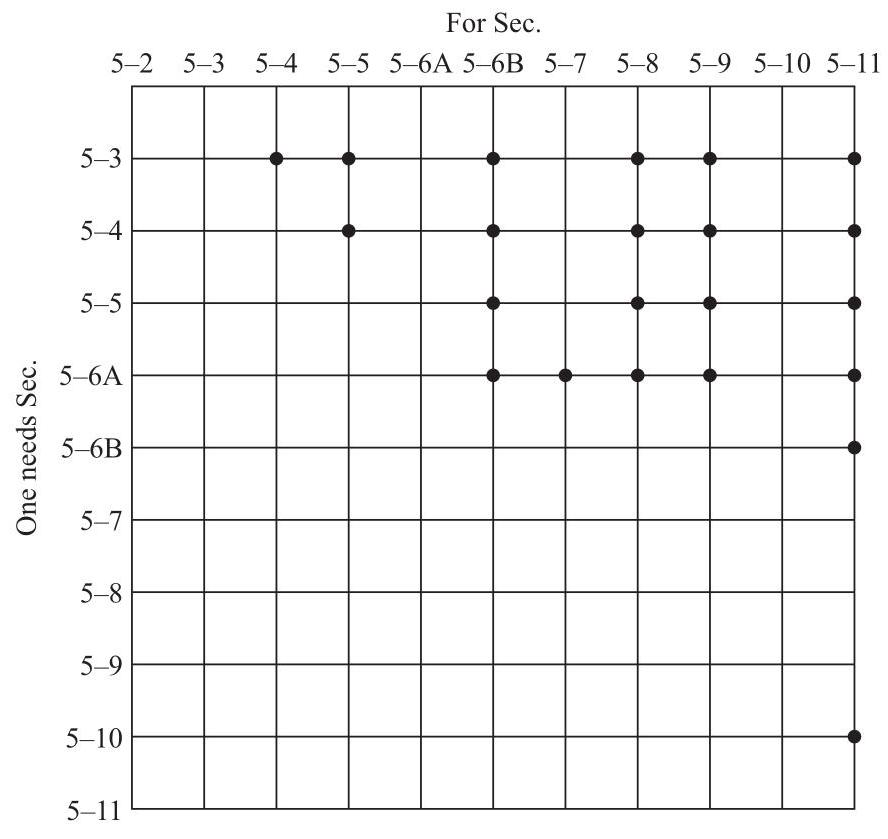
\includegraphics[max width=0.8\textwidth]{images/bo_d4b9jf3ef24c73e0334g_333_319_1328_888_839_0.jpg}
\end{center}
\hspace*{3em} 

5-2. 球面的刚性

在第 5-10 节中，我们将引入抽象曲面的概念，并将第 4 章的内蕴几何推广到这类曲面.除了练习题，本节完全独立于前面的章节.在本节末尾，我们将提及可能的进一步推广，例如可微流形和黎曼流形.

在第 5-11 节中，我们将证明希尔伯特定理，该定理意味着在 \({R}^{3}\) 中不存在具有常负高斯曲率的完备正则曲面.

在附带的图表中，我们给出了本章各节的依赖关系表.例如，第 5-11 节需要第 5-3、5-4、5-5、5-6 和 5-10 节；第 5-7 节需要第 5-6 节 A 部分；第 5-8 节需要第 5-3、5-4 和 5-5 节以及第 5-6 节 A 部分.

\section*{5-2. 球面的刚性}

也许从一个典型的、尽管简单的全局定理例子开始是方便的.我们选择球面的刚性.

我们将证明球面是刚性的，具体含义如下.设 \(\varphi  : \sum  \rightarrow  S\) 是一个球面 \(\sum  \subset  {R}^{3}\) 到一个正则曲面 \(S = \; \varphi \left( \sum \right)  \subset  {R}^{3}\) 的等距映射.那么 \(S\) 是一个球面.直观地说，这意味着不可能使一个由柔韧但无弹性的材料制成的球变形.

实际上，我们将证明以下定理.

定理 1. 设 S 是一个紧致、连通、正则曲面，其高斯曲率为常数 K.则 S 是一个球面.

球体的刚性可由定理 1 直接得出.事实上，设 \(\varphi  : \sum  \rightarrow  S\) 是球面 \(\sum\) 到 \(S\) 的一个等距映射.那么，由于曲率在等距映射下不变， \(\varphi \left( \sum \right)  = S\) 具有常曲率.此外，由于 \(\varphi \left( \sum \right)  = S\) 是紧致且连通集 \(\sum\) 的连续像(附录第 5 章，命题 6 和 12)，因此 \(\varphi \left( \sum \right)  = S\) 是紧致且连通的.由定理 1 可知， \(S\) 是一个球面.

定理 1 的第一个证明由 H. Liebmann (1899) 完成.我们在此提出的证明是 S. S. Chern 对 D. Hilbert 的一个证明的修改(S. S. Chern，“欧几里得球体的若干新刻画”，Duke Math. J. 12 (1945)，270-290；以及 D. Hilbert，Grundlagen der Geometrie，第 3 版，莱比锡，1909，附录 5).

注 1. 应该注意到，存在与球面同胚但并非刚性的曲面.图 5-1 给出了一个例子.我们将图 5-1 中曲面 \(S\) 的平面区域 \(P\) 替换为一个向内的“凸起”，使得所得曲面 \({S}^{\prime }\) 仍然是规则的.由“对称凸起”形成的曲面 \({S}^{\prime \prime }\) 与 \({S}^{\prime }\) 等距，但不存在一个线性正交变换将 \({S}^{\prime }\) 映射到 \({S}^{\prime \prime }\) .因此， \({S}^{\prime }\) 不是刚性的.

\begin{center}
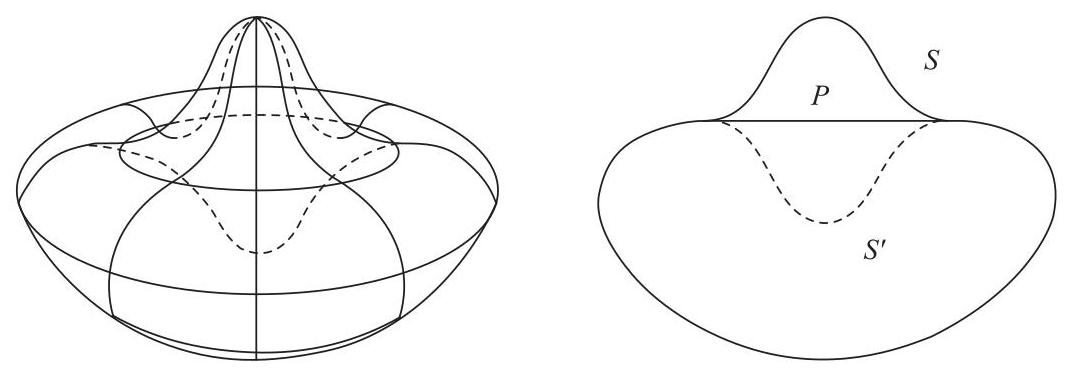
\includegraphics[max width=0.9\textwidth]{images/bo_d4b9jf3ef24c73e0334g_335_230_189_1072_370_0.jpg}
\end{center}
\hspace*{3em} 

图 5-1

我们回顾以下约定.我们选择主曲率 \({k}_{1}\) 和 \({k}_{2}\) ，使得对于每一个 \(q \in  S\) 都有 \({k}_{1}\left( q\right)  \geq  {k}_{2}\left( q\right)\) .通过这种方式，我们得到 \({k}_{1}\) 和 \({k}_{2}\) 作为 \(S\) 中的连续函数，它们除了可能在 \(S\) 的脐点 \(\left( {{k}_{1} = {k}_{2}}\right)\) 处之外是可微的.

定理 1 的证明基于以下局部引理，我们将使用 Mainardi-Codazzi 方程(第 4-3 节).

引理 1. 设 \(S\) 是一个规则曲面， \(\mathrm{p} \in  S\) 是 \(S\) 上的一点，满足以下条件:

1. \(\mathrm{K}\left( \mathrm{p}\right)  > 0\) ；即， \(\mathrm{p}\) 处的高斯曲率为正.

2. \(\mathrm{p}\) 同时是函数 \({\mathrm{k}}_{1}\) 的局部最大点和函数 \({\mathrm{k}}_{2}\left( {{\mathrm{k}}_{1} \geq  {\mathrm{k}}_{2}}\right)\) 的局部最小点.

那么 \(\mathrm{p}\) 是 \(S\) 的脐点.

证明.假设 \(p\) 不是脐点，并导出矛盾.

如果 \(p\) 不是 \(S\) 的脐点，则可以通过坐标 \(\left( {u,v}\right)\) 来参数化 \(p\) 的邻域，使得坐标线是曲率线(第 3-4 节).在这种情况下， \(F = f = 0\) ，并且主曲率由 \(e/E,g/G\) 给出.由于点 \(p\) 不是脐点，我们可以假设，通过必要时交换 \(u\) 和 \(v\) ，在 \(p\) 的邻域内

\[
{k}_{1} = \frac{e}{E},\;{k}_{2} = \frac{g}{G}. \tag{1}
\]

在由此得到的坐标系中，Mainardi-Codazzi 方程写为(第 4-3 节，方程 (7) 和 (7a))

\[
{e}_{v} = \frac{{E}_{v}}{2}\left( {{k}_{1} + {k}_{2}}\right) , \tag{2}
\]

\[
{g}_{u} = \frac{{G}_{u}}{2}\left( {{k}_{1} + {k}_{2}}\right) . \tag{3}
\]

通过对方程 (1) 的第一个方程关于 \(v\) 求导，并使用方程 (2)，我们得到

\[
E{\left( {k}_{1}\right) }_{v} = \frac{{E}_{v}}{2}\left( {-{k}_{1} + {k}_{2}}\right) . \tag{4}
\]

类似地，通过对 (1) 的第二个方程关于 \(u\) 求导，并使用公式 (3)，

\[
G{\left( {k}_{2}\right) }_{u} = \frac{{G}_{u}}{2}\left( {{k}_{1} - {k}_{2}}\right) . \tag{5}
\]

另一方面，当 \(F = 0\) 时， \(K\) 的高斯公式简化为 (见第 4-3 节，练习 1)

\[
K =  - \frac{1}{2\sqrt{EG}}\left\{  {{\left( \frac{{E}_{v}}{\sqrt{EG}}\right) }_{v} + {\left( \frac{{G}_{u}}{\sqrt{EG}}\right) }_{u}}\right\}  ;
\]

因此，

\[
- {2KEG} = {E}_{vv} + {G}_{uu} + M{E}_{v} + N{G}_{u}, \tag{6}
\]

其中 \(M = M\left( {u,v}\right)\) 和 \(N = N\left( {u,v}\right)\) 是 \(\left( {u,v}\right)\) 的函数，它们的表达式对于证明来说无关紧要.同样的说明也适用于下面将要引入的 \(\bar{M},\bar{N},\widetilde{M}\) 和 \(\widetilde{N}\) .

从公式 (4) 和 (5) 中，我们得到 \({E}_{v}\) 和 \({G}_{u}\) 的表达式，将它们求导并代入公式 (6) 中，得到

\[
- {2KEG} =  - \frac{2E}{{k}_{1} - {k}_{2}}{\left( {k}_{1}\right) }_{vv} + \frac{2G}{{k}_{1} - {k}_{2}}{\left( {k}_{2}\right) }_{uu} + \bar{M}{\left( {k}_{1}\right) }_{v} + \bar{N}{\left( {k}_{2}\right) }_{u};
\]

因此，

\[
- 2\left( {{k}_{1} - {k}_{2}}\right) {KEG} =  - {2E}{\left( {k}_{1}\right) }_{vv} + {2G}{\left( {k}_{2}\right) }_{uu} + \widetilde{M}{\left( {k}_{1}\right) }_{v} + \widetilde{N}{\left( {k}_{2}\right) }_{u}. \tag{7}
\]

由于 \(K > 0\) 和 \({k}_{1} > {k}_{2}\) 在 \(p\) 处，公式 (7) 的左侧在 \(p\) 处严格为负.由于 \({k}_{1}\) 在 \(p\) 处达到局部最大值，而 \({k}_{2}\) 在 \(p\) 处达到局部最小值，我们有

\[
{\left( {k}_{1}\right) }_{v} = 0,\;{\left( {k}_{2}\right) }_{u} = 0,\;{\left( {k}_{1}\right) }_{vv} \leq  0,\;{\left( {k}_{2}\right) }_{uu} \geq  0
\]

在 \(p\) 处.然而，这意味着公式 (7) 的右侧为正或零，这是一个矛盾.引理 1 证毕.Q.E.D.

应该注意的是，如果我们假设 \({k}_{1}\) 在 \(p\) 处有局部最小值，而 \({k}_{2}\) 在 \(p\) 处有局部最大值，那么在证明中不会出现矛盾.实际上，这种情况可能发生在曲率为正的曲面上，而 \(p\) 不是脐点，如下例所示.

例 1. 令 \(S\) 为一个旋转曲面，其方程为 (参见第 3-3 节，例 4)

\[
x = \varphi \left( v\right) \cos u,\;y = \varphi \left( v\right) \sin u,\;z = \psi \left( v\right) ,\;0 < u < {2\pi },
\]

其中

\[
\varphi \left( v\right)  = C\cos v,\;C > 1,
\]

\[
\psi \left( v\right)  = \int \sqrt{1 - {C}^{2}{\sin }^{2}v}{dv},\;\psi \left( 0\right)  = 0.
\]

我们取 \(\left| v\right|  < {\sin }^{-1}\left( {1/C}\right)\) ，使得 \(\psi \left( v\right)\) 有定义.

利用已知的表达式 (参见第 3-3 节，例 4)，我们得到

\[
E = {C}^{2}{\cos }^{2}v
\]

\[
F = 0,
\]

\[
G = 1,
\]

\[
e =  - C\cos v\left( \sqrt{1 - {C}^{2}{\sin }^{2}v}\right)
\]

\[
f = 0
\]

\[
g =  - \frac{C\cos v}{\sqrt{1 - {C}^{2}{\sin }^{2}v}}
\]

因此，

\[
{k}_{1} = \frac{e}{E} =  - \frac{\sqrt{1 - {C}^{2}{\sin }^{2}v}}{C\cos v},\;{k}_{2} = \frac{g}{G} =  - \frac{C\cos v}{\sqrt{1 - {C}^{2}{\sin }^{2}v}}.
\]

因此， \(S\) 的曲率为 \(K = {k}_{1}{k}_{2} = 1 > 0\) ，为正且恒定 (参见第 3-3 节，练习 7).

很容易看出 \({k}_{1} > {k}_{2}\) 在 \(S\) 的所有地方，因为 \(C > 1\) .因此， \(S\) 没有脐点.此外，由于 \({k}_{1} =  - \left( {1/C}\right)\) 对于 \(v = 0\) ，并且

\[
{k}_{1} =  - \frac{\sqrt{1 - {C}^{2}{\sin }^{2}v}}{C\cos v} >  - \frac{1}{C}\;\text{ for }v \neq  0,
\]

我们得出结论， \({k}_{1}\) 达到最小值(因此 \({k}_{2}\) 达到最大值，因为 \(K = 1\) )，在平行 \(v = 0\) 的点上.

顺便说一句，这个例子表明定理 1 中的紧致性假设是必不可少的，因为曲面 \(S\) (见图 5-2)具有恒定的正曲率，但不是球面.

在定理 1 的证明中，我们将使用以下事实，并将其建立为一个引理.

\begin{center}
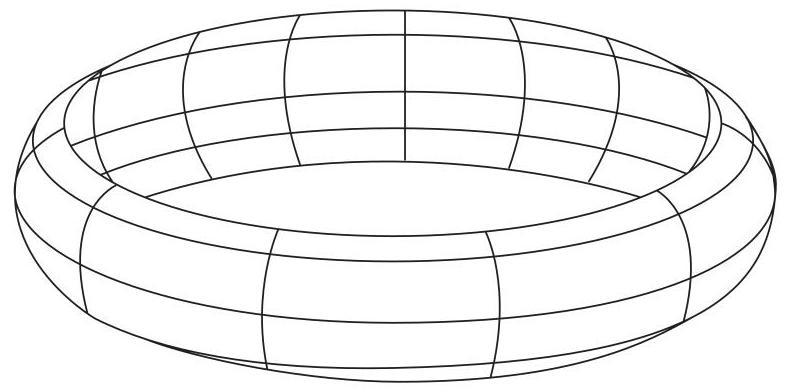
\includegraphics[max width=0.7\textwidth]{images/bo_d4b9jf3ef24c73e0334g_338_388_196_789_388_0.jpg}
\end{center}
\hspace*{3em} 

图 5-2

引理 2. 一个正则紧致曲面 \(S \subset  {\mathbb{R}}^{3}\) 至少有一个椭圆点.

证明.由于 \(S\) 是紧致的， \(S\) 是有界的.因此，存在半径为 \({R}^{3}\) 、中心固定在点 \(O \in  {R}^{3}\) 的球面，使得 \(S\) 包含在其中任何一个球面所围区域的内部.考虑所有这些球面的集合.设 \(r\) 为它们半径的下确界，设 \(\sum  \subset  {R}^{3}\) 为半径为 \(r\) 、中心在 \(O\) 的球面.显然， \(\sum\) 和 \(S\) 至少有一个公共点，记为 \(p\) . \(\sum\) 在 \(p\) 处的切平面在 \(p\) 的邻域内仅与 \(S\) 有公共点 \(p\) .因此， \(\sum\) 和 \(S\) 在 \(p\) 处相切.通过观察 \(p\) 处的法截面，很容易得出 \(S\) 在 \(p\) 处的任何法曲率都大于或等于 \(\sum\) 在 \(p\) 处的相应曲率.因此， \({K}_{S}\left( p\right)  \geq  {K}_{\sum }\left( p\right)  > 0\) ，并且 \(p\) 是一个椭圆点，正如我们所希望的.Q.E.D.

定理 1 的证明.由于 \(S\) 是紧致的，根据引理 2，存在一个椭圆点.因为 \(K\) 是常数， \(K > 0\) 在 \(S\) 中.

根据紧致性，连续函数 \({k}_{1}\) 在 \(S\) 上在点 \(p \in  S\) 处达到最大值(附录第 5 章，命题 13).因为 \(K = {k}_{1}{k}_{2}\) 是一个正常数， \({k}_{2}\) 是 \({k}_{1}\) 的减函数，因此它在 \(p\) 处达到最小值.从引理 1 可知， \(p\) 是一个脐点；也就是说， \({k}_{1}\left( p\right)  = \; {k}_{2}\left( p\right)\) .

现在设 \(q\) 是 \(S\) 的任意给定点.因为我们假设 \({k}_{1}\left( q\right)  \geq  {k}_{2}\left( q\right)\) ，所以我们有

\[
{k}_{1}\left( p\right)  \geq  {k}_{1}\left( q\right)  \geq  {k}_{2}\left( q\right)  \geq  {k}_{2}\left( p\right)  = {k}_{1}\left( p\right) .
\]

因此，对于每一个 \(q \in  S\) ，都有 \({k}_{1}\left( q\right)  = {k}_{2}\left( q\right)\) .

由此可知， \(S\) 的所有点都是脐点，根据 3-2 节的命题 4， \(S\) 包含在一个球面或平面中.因为 \(K > 0,S\) 包含在一个球面 \(\sum\) 中.根据紧致性， \(S\) 在 \(\sum\) 中是闭合的，并且因为 \(S\) 是一个正则曲面， \(S\) 在 \(\sum\) 中是开放的.因为 \(\sum\) 是连通的，并且 \(S\) 在 \(\sum ,S = \sum\) 中是开放的和闭合的(附录第 5 章，命题 5).

因此，曲面 \(S\) 是一个球面.Q.E.D.

注意到定理1的证明中，仅使用 \(K = {k}_{1}{k}_{2}\) 为常数的假设来保证 \({k}_{2}\) 是 \({k}_{1}\) 的减函数.如果我们假设平均曲率 \(H = \; \frac{1}{2}\left( {{k}_{1} + {k}_{2}}\right)\) 为常数，也能得出相同的结论.这允许我们陈述

定理1a.设 \(S\) 为一个正则、紧致且连通的曲面，其高斯曲率为 \(\mathrm{K} > 0\) ，平均曲率为 \(\mathrm{H}\) 常数.则 \(S\) 是一个球面.

证明与定理1的证明完全类似.实际上，该论证适用于 \({k}_{2} = f\left( {k}_{1}\right)\) ，其中 \(f\) 是 \({k}_{1}\) 的减函数.更精确地说，我们有

定理1b.设S为一个具有正高斯曲率的正则、紧致且连通的曲面.如果存在一个关系 \({\mathrm{k}}_{2} = \mathrm{f}\left( {\mathrm{k}}_{1}\right)\) 在 \(S\) 中，其中 \(\mathrm{f}\) 是 \({\mathrm{k}}_{1},{\mathrm{k}}_{1} \geq  {\mathrm{k}}_{2}\) 的减函数，则 \(S\) 是一个球面.

注2.高斯曲率为 \(K > 0\) 的紧致连通曲面 \({R}^{3}\) 称为卵形面.因此，定理1a可以陈述如下:平均曲率为常数的卵形面是一个球面.

另一方面，根据Gauss-Bonnet定理，卵形面同胚于球面(参见第4-5节，应用1).H. Hopf证明了定理1a仍然成立，其(更强的)陈述如下:平均曲率为常数且同胚于球面的正则曲面是一个球面.A. Alexandroff的一个定理通过用紧致性替换同胚于球面的条件，进一步推广了这个结果:平均曲率为常数的正则、紧致且连通的曲面是一个球面.

上述结果的阐述可以在Hopf [11]中找到.(参考文献列在书末.)

注3.球面的刚性可以作为卵形面一般刚性定理的一个推论得到.这个由Cohn-Vossen提出的定理指出:两个等距的卵形面相差一个 \({R}^{3}\) 的正交线性变换.这个结果的证明可以在Chern [10]中找到.

定理1是全局微分几何的一个典型结果，即局部实体的信息(在此情况下是曲率)加上弱的全局假设(在此情况下是紧致性和连通性)对整个曲面(在此情况下是球面)产生了强烈的限制.注意到连通性的唯一作用是防止在定理1的结论中出现两个或多个球面.另一方面，紧致性的假设在几个方面都是必不可少的，其作用之一是确保我们得到一个完整的球面而不是一个包含在球面内的曲面.

\exerciseline

1.设 \(S \subset  {R}^{3}\) 为一个紧致正则曲面，并固定一点 \({p}_{0} \in  {R}^{3},{p}_{0} \notin  S\) .设 \(d : S \rightarrow  R\) 是由 \(d\left( q\right)  = \frac{1}{2}{\left| q - {p}_{0}\right| }^{2}\) 定义的微分函数， \(q \in  S\) .由于 \(S\) 是紧致的，存在 \({q}_{0} \in  S\) 使得对于所有 \(q \in  S\) 都有 \(d\left( {q}_{0}\right)  \geq  d\left( q\right)\) .证明 \({q}_{0}\) 是 \(S\) 的一个椭圆点(这提供了引理2的另一个证明).

2. 设 \(S \subset  {R}^{3}\) 为一个高斯曲率为 \(K > 0\) 且无脐点的正则曲面.证明在 \(S\) 上不存在一点，使得 \(H\) 达到最大值且 \(K\) 达到最小值.

3. (卡兹丹-沃纳的注记.) 令 \(S \subset  {R}^{3}\) 为由旋转曲线得到的延拓紧致旋转曲面(参见第 2-3 节注记 4)

\[
\alpha \left( s\right)  = \left( {0,\varphi \left( s\right) ,\psi \left( s\right) }\right) ,
\]

参数化由弧长 \(s \in  \left\lbrack  {0,l}\right\rbrack\) 给出，绕 \(z\) 轴旋转.此处对于所有 \(s \in  \left\lbrack  {0,l}\right\rbrack\) 均有 \(\varphi \left( 0\right)  = \varphi \left( l\right)  = 0\) 和 \(\varphi \left( s\right)  > 0\) .极点的 \(S\) 的正则性进一步意味着 \({\varphi }^{\prime }\left( 0\right)  = 1,{\varphi }^{\prime }\left( l\right)  =  - 1\) (参见第 2-3 节练习 10).我们也知道 \(S\) 的高斯曲率由 \(K =  - {\varphi }^{\prime \prime }\left( s\right) /\varphi \left( s\right)\) 给出(参见第 3-3 节例 4).

*a. 证明

\[
{\int }_{0}^{t}{K}^{\prime }{\varphi }^{2}{ds} = 0,\;{K}^{\prime } = \frac{dK}{ds}.
\]

b. 从 a 部分得出结论，在 \({R}^{3}\) 中不存在具有单调递增曲率的紧致(延拓)回转曲面.

以下练习概述了 Hopf 定理的证明:一个具有常数平均曲率且同胚于球面的正则曲面是一个球面(参见注记 2).Hopf 的主要思想在近期的工作中被反复使用.该练习需要一些关于复变函数的基本事实.

4. 设 \(U \subset  {R}^{3}\) 是 \({R}^{2}\) 的一个开连通子集，设 \(\mathbf{x} : U \rightarrow  S\) 是正则曲面 \(S\) 的一个等温参数化(即 \(E = G,F = 0\) ；参见第 4-2 节).我们通过令 \(u + {iv} = \zeta\) 来将 \({R}^{2}\) 与复平面 \(\mathbb{C}\) 识别， \(\left( {u,v}\right)  \in  {R}^{2},\zeta  \in  \mathbb{C}.\zeta\) 被称为对应于 \(\mathbf{x}\) 的复参数.设 \(\phi  : \mathbf{x}\left( U\right)  \rightarrow  \mathbb{C}\) 是由下式给出的复值函数

\[
\phi \left( \zeta \right)  = \phi \left( {u,v}\right)  = \frac{e - g}{2} - {if} = {\phi }_{1} + i{\phi }_{2},
\]

其中 \(e,f,g\) 是 \(S\) 的第二基本形式的系数.

a. 证明在等温参数化 \(\mathbf{x}\) 下，Mainardi-Codazzi 方程(参见第 4-3 节)可以写成

\[
{\left( \frac{e - g}{2}\right) }_{u} + {f}_{v} = E{H}_{u},\;{\left( \frac{e - g}{2}\right) }_{v} - {f}_{u} =  - E{H}_{v}
\]

并得出结论， \(\mathbf{x}\left( U\right)  \subset  S\) 的平均曲率 \(H\) 是常数当且仅当 \(\phi\) 是 \(\zeta\) 的解析函数(即 \({\left( {\phi }_{1}\right) }_{u} = {\left( {\phi }_{2}\right) }_{v},{\left( {\phi }_{1}\right) }_{v} = \; \left. {-{\left( {\phi }_{2}\right) }_{u}}\right)\) .

b. 定义“复导数”

\[
\frac{\partial }{\partial \zeta } = \frac{1}{2}\left( {\frac{\partial }{\partial u} - i\frac{\partial }{\partial v}}\right) ,
\]

并证明 \(\phi \left( \zeta \right)  =  - 2\left\langle  {{\mathbf{x}}_{\zeta },{N}_{\zeta }}\right\rangle\) ，其中 \({\mathbf{x}}_{\zeta }\) 例如表示具有复数坐标的向量

\[
{\mathbf{x}}_{\zeta } = \left( {\frac{\partial x}{\partial \zeta },\frac{\partial y}{\partial \zeta },\frac{\partial z}{\partial \zeta }}\right) .
\]

c. 设 \(f : U \subset  \mathbb{C} \rightarrow  V \subset  \mathbb{C}\) 是一个由 \(f\left( {u + {iv}}\right)  = x + {iy} = \eta\) 定义的一一复函数.证明 \(\left( {x,y}\right)\) 是 \(S\) 上的等温参数(即 \(\eta\) 是 \(S\) 上的复参数)，当且仅当 \(f\) 是解析的且 \({f}^{\prime }\left( \zeta \right)  \neq  0,\zeta  \in  U\) .设 \(\mathbf{y} = \mathbf{x} \circ  {f}^{-1}\) 是相应的参数化，并定义 \(\psi \left( \eta \right)  =  - 2\left\langle  {{\mathbf{y}}_{\eta },{N}_{\eta }}\right\rangle\) .证明在 \(\mathbf{x}\left( U\right)  \cap  \mathbf{y}\left( V\right)\) 上

\[
\phi \left( \zeta \right)  = \psi \left( \eta \right) {\left( \frac{\partial \eta }{\partial \zeta }\right) }^{2}.
\]
 (*)

d. 令 \({S}^{2}\) 为 \({R}^{3}\) 的单位球面.使用立体投影(参见练习 16，第 2-2 节)从极点 \(N = \left( {0,0,1}\right)\) 和 \(S = \left( {0,0, - 1}\right)\) 将 \({S}^{2}\) 用两个(等温)复参数 \(\zeta\) 和 \(\eta\) 的坐标邻域覆盖，其中包含 \(\zeta \left( S\right)  = 0\) 和 \(\eta \left( N\right)  = 0\) ，使得在这些坐标邻域的交集 \(W\) (球面减去两个极点)中， \(\eta  = {\zeta }^{-1}\) .假设在每个坐标邻域上都存在解析函数 \(\varphi \left( \zeta \right) ,\psi \left( \eta \right)\) ，使得在 \(W\) 中成立 \(\left( *\right)\) .使用刘维尔定理证明 \(\varphi \left( \zeta \right)  \equiv  0\) (因此， \(\psi \left( \eta \right)  \equiv  0\) ).

e. 设 \(S \subset  {R}^{3}\) 是一个具有常平均曲率且同胚于球面的正则曲面.假设存在一个共形微分同胚 \(\varphi  : S \rightarrow  {S}^{2}\) 将 \(S\) 映射到单位球面 \({S}^{2}\) (这是黎曼曲面均匀化定理的一个结果，在此假设).设 \(\widetilde{\zeta }\) 和 \(\widetilde{\eta }\) 是在 \(\varphi\) 下与 d 部分中给出的 \({S}^{2}\) 的参数 \(\zeta\) 和 \(\eta\) 相对应的复参数.根据 a 部分，函数 \(\phi \left( \widetilde{\zeta }\right)  = \left( {\left( {e - g}\right) /2}\right)  - {if}\) 是解析的.类似的函数 \(\psi \left( \widetilde{\eta }\right)\) 也是解析的，并且根据 \(c\) 部分，它们的关系是 \(\left( *\right)\) .使用 \(d\) 部分证明 \(\phi \left( \widetilde{\zeta }\right)  \equiv  0\) (因此， \(\psi \left( \widetilde{\eta }\right)  \equiv  0\) ).由此得出 \(S\) 由脐点组成，因此是一个球面.这证明了霍普夫定理.

\section*{5-3. 完全曲面.霍普夫-林诺夫定理}

从现在开始，除非另有说明，所有将要考虑的曲面都是正则且连通的.

5-2节末尾的考虑表明，为了获得全局定理，除了连通性之外，我们还需要一些全局假设来确保曲面不能作为正则曲面被“扩展”.显然，紧致性可以达到这个目的.然而，拥有一个比紧致性更弱但仍能产生相同效果的假设将是有用的.这将使我们能够在比紧致性更一般的情况下预期全局定理.

以下定义对曲面不可扩展的概念给出了更精确的表述.

定义 1. 若存在一个正则(连通)曲面 \(\overline{S}\) ，使得正则(连通)曲面 \(S\) 是 \(S \subset  \overline{S}\) 的真子集，则称 \(S\) 是可扩展的.若不存在这样的 \(\overline{S}\) ，则称 \(S\) 是不可扩展的.

不幸的是，不可扩展曲面的类别太大，无法得出有趣的结论.一个更合适的假设由以下给出:

定义 2. 当对于每一点 \(\mathrm{p} \in  S\) ，从 \(\mathrm{p} = \gamma \left( 0\right)\) 开始的 \(S\) 的任意参数化测地线 \(\gamma  : \lbrack 0,\epsilon ) \rightarrow  S\) 都可以扩展为在整个直线 R 上定义的参数化测地线 \(\widetilde{\gamma } : \mathbb{R} \rightarrow  S\) 时，称正则曲面 \(S\) 是完备的.

换句话说，当对于每一点 \(\mathrm{p} \in  S\) ，映射 \({\exp }_{\mathrm{p}} : {\mathrm{T}}_{\mathrm{p}}\left( S\right)  \rightarrow  S\) (第 4-6 节)对于每一点 \(\mathrm{v} \in  {\mathrm{T}}_{\mathrm{p}}\left( S\right)\) 都有定义时， \(S\) 就是完备的.

我们将在后面证明(命题 1)每个完备曲面都是不可扩展的，并且存在不可扩展但非完备的曲面(例 1).因此，完备性的假设比不可扩展性的假设更强.此外，我们将证明(命题 5) \({R}^{3}\) 中的每个闭曲面都是完备的；也就是说，完备性的假设比紧致性的假设更弱.

本节的目的是证明，给定一个完备曲面 \(S\) 上的两点 \(p,q \in  S\) ，存在一条连接 \(p\) 和 \(q\) 的测地线是极小的(即其长度小于或等于连接 \(p\) 和 \(q\) 的任何其他曲线的长度).这个基本结果首先由 Hopf 和 Rinow 证明(H. Hopf, W. Rinow, "Über den Begriff der vollständigen differentialgeometriscben Flächen," Comm. Math. Helv. 3 (1931), 209-225).这个定理是完备曲面比不可扩展曲面更适合微分几何的主要原因.

现在我们来看一些例子.平面显然是一个完备曲面.去掉顶点的圆锥体是一个非完备曲面，因为通过充分扩展一条生成线(这是一条测地线)，我们可以到达不属于该曲面的顶点.球体是一个完备曲面，因为它的参数化测地线(其轨迹是球体的大圆)可以为所有实数值定义.圆柱体也是一个完备曲面，因为它的测地线是圆、直线和螺旋线，它们对所有实数值都有定义.

另一方面，从一个完整的曲面 \(S\) 中移除一个点 \(p\) 所得到的曲面 \(S - \{ p\}\) 不是完整的.事实上， \(S\) 的一条测地线 \(\gamma\) 应该经过 \(p\) .通过取一点 \(q\) ，在 \(\gamma\) 上靠近 \(p\) 的地方(图 5-3)，存在一个参数化的 \(S - \{ p\}\) 的测地线，它从 \(q\) 开始，但不能通过 \(p\) 延拓(这个论证将在命题 1 中详细给出).因此，一个点去掉后的球面和一个点去掉后的圆柱体都不是完整的曲面.

\begin{center}
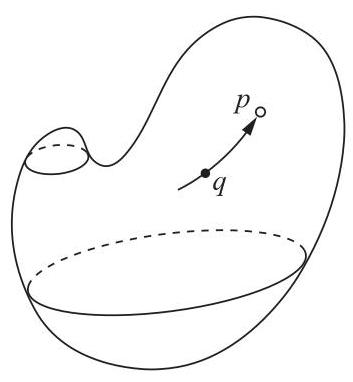
\includegraphics[max width=0.3\textwidth]{images/bo_d4b9jf3ef24c73e0334g_343_183_914_353_382_0.jpg}
\end{center}
\hspace*{3em} 

图 5-3

命题 1. 一个完整的曲面 \(S\) 是不可延拓的.

证明. 假设 \(S\) 是可延拓的，并导出矛盾. 说 \(S\) 是可延拓的，意味着存在一个正则(连通)曲面 \(\bar{S}\) 具有 \(S \subset  \bar{S}\) . 由于 \(S\) 是一个正则曲面， \(S\) 在 \(\bar{S}\) 中是开集. \(S\) 在 \(\bar{S}\) 中的边界(第 5 章附录，定义 4)Bd \(S\) 非空；否则 \(\bar{S} = S \cup  \left( {\bar{S} - S}\right)\) 将是两个不相交的开集 \(S\) 和 \(\bar{S} - S\) 的并集，这与 \(\bar{S}\) 的连通性(第 5 章附录，定义 10)矛盾. 因此，存在一点 \(p \in  \operatorname{Bd}S\) , 并且由于 \(S\) 在 \(\bar{S},p \notin  S\) 中是开集.

设 \(\bar{V} \subset  \bar{S}\) 是 \(\bar{S}\) 中 \(p\) 的一个邻域，使得每个 \(q \in  \bar{V}\) 都可以通过 \(\bar{S}\) 的唯一测地线与 \(p\) 连接(第 4-6 节，命题 2). 由于 \(p \in  \operatorname{Bd}S\) , 某个 \({q}_{0} \in  \bar{V}\) 属于 \(S\) . 设 \(\overline{\gamma } : \left\lbrack  {0,1}\right\rbrack   \rightarrow  \bar{S}\) 是 \(S\) 的一条测地线，具有 \(\overline{\gamma }\left( 0\right)  = p\) 和 \(\overline{\gamma }\left( 1\right)  = {q}_{0}\) . 显然， \(\alpha  : \lbrack 0,\epsilon ) \rightarrow  S\) , 由 \(\alpha \left( t\right)  = \overline{\gamma }\left( {1 - t}\right)\) 给出，是 \(S\) 的一条测地线，其 \(\alpha \left( 0\right)  = {q}_{0}\) , 延拓到直线 \(R\) 将穿过 \(p\) 对于 \(t = 1\) (图 5-4). 由于 \(p \notin  S\) , 这条测地线不能延拓，这与完备性的假设矛盾，并结束证明. Q.E.D.

\begin{center}
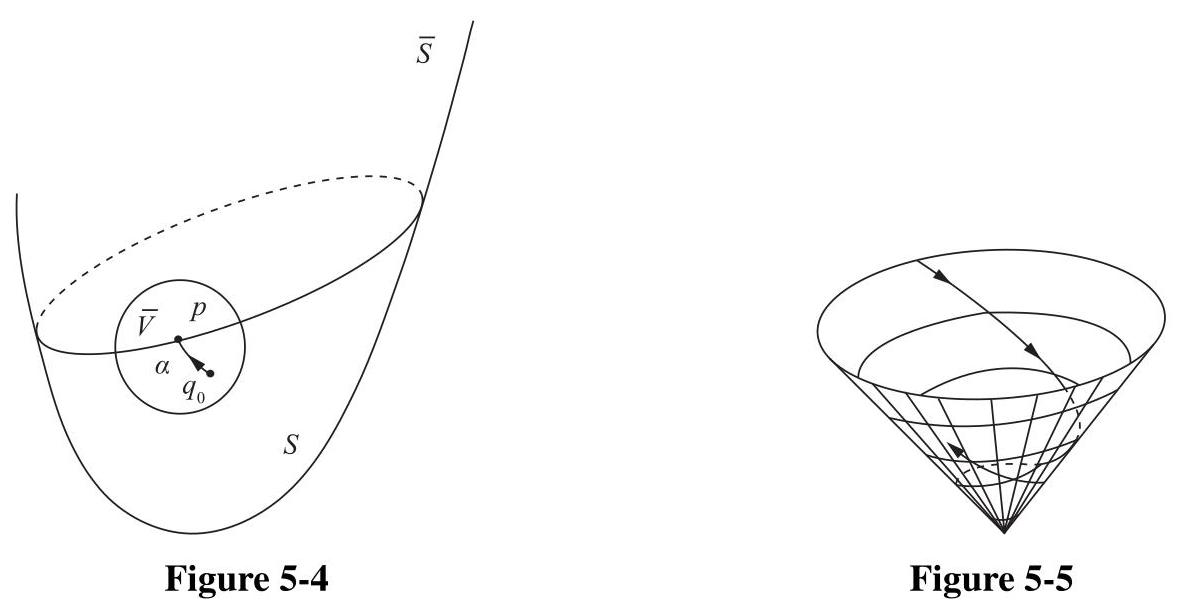
\includegraphics[max width=1.0\textwidth]{images/bo_d4b9jf3ef24c73e0334g_344_195_185_1185_613_0.jpg}
\end{center}
\hspace*{3em} 

命题 1 的逆命题是错误的，如下例所示.

例 1. 当我们从由下式给出的单叶锥中移除顶点 \({p}_{0}\) 时

\[
z = \sqrt{{x}^{2} + {y}^{2}},\;\left( {x,y}\right)  \in  {R}^{2},
\]

我们得到一个正则曲面 \(S.S\) 不完整，因为生成线在任意弧长值下都无法延拓而不到达顶点.

我们通过假设 \(S \subset  \bar{S}\) , 其中 \(\bar{S} \neq  S\) 是一个正则曲面，并导出矛盾来证明 \(S\) 是不可延拓的. 该论证包括证明 \(S\) 在 \(\bar{S}\) 中的边界简化为顶点 \({p}_{0}\) , 并且存在 \(\bar{S}\) 中 \({p}_{0}\) 的一个邻域 \(\bar{W}\) , 使得 \(\bar{W} - \left\{  {p}_{0}\right\}   \subset  S\) . 但这与锥体(包含顶点 \({p}_{0}\) )在 \({p}_{0}\) 中不是正则曲面(第 2-2 节，例 5)这一事实相矛盾.

首先，我们观察到 \(S\) 中唯一一条从点 \(p \in  S\) 开始的测地线，对于参数的任意值都不能延拓，那就是通过 \(p\) 的子午线(生成线)(见图 5-5). 通过使用，例如，克莱罗关系(第 4-4 节，例 5)，可以很容易地看出这一点，并将留作练习(练习 2).

现在令 \(p \in  \operatorname{Bd}S\) ，其中 \(\operatorname{Bd}S\) 表示 \(\bar{S}\) 中的 \(S\) 的边界(正如我们在命题 1，Bd \(S \neq  \phi\) 中所见).由于 \(S\) 是 \(\bar{S},p \notin  S\) 中的一个开集.令 \(\bar{V}\) 是 \(\bar{S}\) 中 \(p\) 的一个邻域，使得 \(\bar{V}\) 的每个点都可以通过 \(\bar{S}\) 在 \(\bar{V}\) 中的唯一测地线与 \(p\) 连接.由于 \(p \in  \operatorname{Bd}S\) ，存在 \(q \in  \bar{V} \cap  S\) .令 \(\overline{\gamma }\) 是连接 \(p\) 和 \(q\) 的 \(\bar{S}\) 的一条测地线.因为 \(S\) 是 \(\bar{S},\overline{\gamma }\) 中的一个开集，它在 \(q\) 的邻域中与 \(S\) 的一条测地线 \(\gamma\) 一致.令 \({p}_{0}\) 是 \(\overline{\gamma }\) 中第一个不属于 \(S\) 的点.根据初步观察， \(\overline{\gamma }\) 是一条经线，而 \({p}_{0}\) 是 \(S\) 的顶点.此外， \({p}_{0} = p\) ；否则，将存在一个不包含 \({p}_{0}\) 的 \(p\) 的邻域.通过重复对该邻域的论证，我们将得到一个不同于 \({p}_{0}\) 的顶点，这是矛盾的.因此，Bd \(S\) 缩减为顶点 \({p}_{0}\) .

现在令 \(\bar{W}\) 是 \(\bar{S}\) 中 \({p}_{0}\) 的一个邻域，使得 \(\bar{W}\) 的任意两点都可以通过 \(\bar{S}\) 的测地线连接(第 4-7 节，命题 1).我们将证明 \(\bar{W} - \left\{  {p}_{0}\right\}   \subset  S\) .事实上， \(\gamma\) 的点属于 \(S\) .另一方面，一个不属于 \(\gamma\) 或其延长线的点 \(r \in  \bar{W}\) 可以通过一条不同于 \(\gamma\) 的测地线 \(\alpha\) 连接到 \(\gamma ,t \neq  {p}_{0},t \in  \bar{W}\) 的一个点 \(t\) (见图 5-6).根据初步观察， \(\alpha\) 的每个点，特别是 \(r\) ，都属于 \(S\) .最后， \(\gamma\) 的延长线的点，除了 \({p}_{0}\) ，也属于 \(S\) ；否则，它们将属于 \(S\) 的边界，而我们已经证明该边界只由 \({p}_{0}\) 组成.

\begin{center}
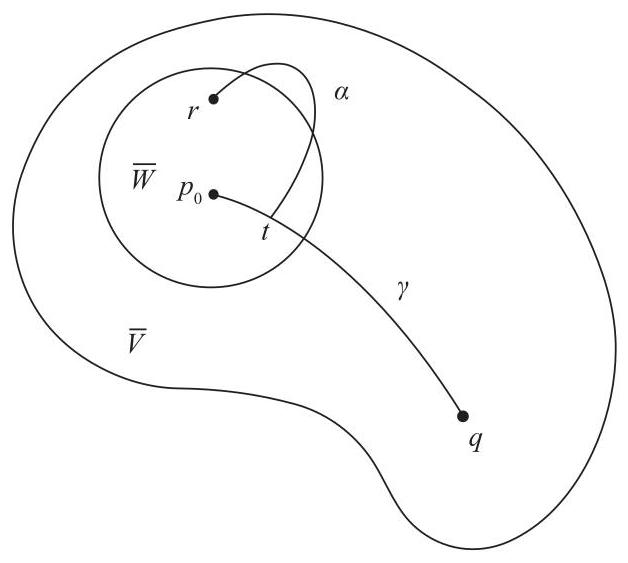
\includegraphics[max width=0.5\textwidth]{images/bo_d4b9jf3ef24c73e0334g_345_180_711_628_563_0.jpg}
\end{center}
\hspace*{3em} 

图 5-6

这样，我们的论断就完全证明了.因此， \(S\) 是不可延拓的，并得到了所需的例子.

对于接下来的内容，引入一个仅取决于 \(S\) 的内在几何形状而不取决于 \(S\) 如何嵌入 \({R}^{3}\) 中的 \(S\) 上两点之间距离的概念是方便的(参见第 4-2 节，注 2).请注意，由于 \(S \subset  {R}^{3}\) ，可以定义 \(S\) 上两点之间的距离，作为这两点在 \({R}^{3}\) 中的距离.然而，这个距离取决于第二基本形式，因此不适用于本章的目的.

我们需要一些准备工作.

一个闭区间 \(\left\lbrack  {a,b}\right\rbrack   \subset  R\) 到直线 \(R\) 的连续映射 \(\alpha  : \left\lbrack  {a,b}\right\rbrack   \rightarrow  S\) 到曲面 \(S\) 被称为连接 \(\alpha \left( a\right)\) 到 \(\alpha \left( b\right)\) 的参数化分段可微曲线，如果存在一个由点 \(a = {t}_{0} < {t}_{1} < {t}_{2} < \cdots  < {t}_{k} < {t}_{k + 1} = b\) 分割的 \(\left\lbrack  {a,b}\right\rbrack\) 的分区，使得 \(\alpha\) 在 \(\left\lbrack  {{t}_{i},{t}_{i + 1}}\right\rbrack\) 中可微， \(i = 0,\ldots ,k\) . \(\alpha\) 的长度 \(l\left( \alpha \right)\) 定义为

\[
l\left( \alpha \right)  = \mathop{\sum }\limits_{{l = 0}}^{k}{\int }_{{t}_{i}}^{{t}_{i + 1}}\left| {{\alpha }^{\prime }\left( t\right) }\right| {dt}
\]

命题 2. 给定一个正则(连通)曲面 \(S\) 上的两点 \(\mathrm{p},\mathrm{q} \in  S\) ，存在一条连接 p 和 q 的参数化分段可微曲线.

证明. 由于 \(S\) 是连通的，存在一条连续曲线 \(\alpha  : \left\lbrack  {a,b}\right\rbrack   \rightarrow  S\) ，其 \(\alpha \left( a\right)  = p,\alpha \left( b\right)  = q\) . 令 \(t \in  \left\lbrack  {a,b}\right\rbrack\) ，令 \({I}_{t}\) 是 \(\left\lbrack  {a,b}\right\rbrack\) 中的一个开区间，包含 \(t\) ，使得 \(\alpha \left( {I}_{t}\right)\) 包含在 \(\alpha \left( t\right)\) 的一个坐标邻域中.并集 \(\cup  {I}_{t},t \in  \left\lbrack  {a,b}\right\rbrack\) 覆盖了 \(\left\lbrack  {a,b}\right\rbrack\) ，并且由于紧致性，有限个 \({I}_{1},\ldots ,{I}_{n}\) 仍然覆盖了 \(\left\lbrack  {a,b}\right\rbrack\) . 因此，可以通过点 \(a = {t}_{0} < {t}_{1} < \cdots  < {t}_{k} < {t}_{k + 1} = b\) 将 \(I\) 分解，使得 \(\left\lbrack  {{t}_{i},{t}_{i + 1}}\right\rbrack\) 包含在某个 \({I}_{j},j = 1,\ldots ,n\) 中.因此， \(\alpha \left( {{t}_{i},{t}_{i + 1}}\right)\) 包含在一个坐标邻域中.

由于 \(p = \alpha \left( {t}_{0}\right)\) 和 \(\alpha \left( {t}_{1}\right)\) 位于同一坐标邻域 \(\mathbf{x}\left( U\right)  \subset  S\) 中，因此可以用一条可微曲线将它们连接起来，即通过 \(\mathbf{x}\) 将连接 \({\mathbf{x}}^{-1}\left( {\alpha \left( {t}_{0}\right) }\right)\) 和 \({\mathbf{x}}^{-1}\left( {\alpha \left( {t}_{1}\right) }\right)\) 的 \(U \subset  {R}^{2}\) 中的一条可微曲线进行映射.通过这个过程，我们用一条可微曲线将 \(\alpha \left( {t}_{i}\right)\) 和 \(\alpha \left( {t}_{i + 1}\right) ,i = 0,\ldots ,k\) 连接起来.这就得到了一条分段可微曲线，连接了 \(p = \alpha \left( {t}_{0}\right)\) 和 \(q = \alpha \left( {t}_{k + 1}\right)\) ，并完成了命题的证明.Q.E.D.

设 \(p,q \in  S\) 为正则曲面 \(S\) 上的两点.我们用 \({\alpha }_{p,q}\) 表示连接 \(p\) 和 \(q\) 的参数化分段可微曲线，用 \(l\left( {\alpha }_{p,q}\right)\) 表示其长度.命题 2 表明所有这样的 \({\alpha }_{p,q}\) 的集合非空.因此，我们可以设定如下:

定义 3. 点 \(\mathrm{p} \in  S\) 到点 \(\mathrm{q} \in  S\) 的(内禀)距离 \(\mathrm{d}\left( {\mathrm{p},\mathrm{q}}\right)\) 是

\[
\mathrm{d}\left( {\mathrm{p},\mathrm{q}}\right)  = \inf \operatorname{l}\left( {\alpha }_{p,q}\right) ,
\]

其中 inf 是在连接 \(\mathrm{p}\) 和 \(\mathrm{q}\) 的所有分段可微曲线上取值.

命题 3. 上述定义的距离 d 具有以下性质，

1. \(\mathrm{d}\left( {\mathrm{p},\mathrm{q}}\right)  = \mathrm{d}\left( {\mathrm{q},\mathrm{p}}\right)\) ,

2. \(\mathrm{d}\left( {\mathrm{p},\mathrm{q}}\right)  + \mathrm{d}\left( {\mathrm{q},\mathrm{r}}\right)  \geq  \mathrm{d}\left( {\mathrm{p},\mathrm{r}}\right)\) ,

3. \(\mathrm{d}\left( {\mathrm{p},\mathrm{q}}\right)  \geq  0\) ,

4. \(\mathrm{d}\left( {\mathrm{p},\mathrm{q}}\right)  = 0\) 当且仅当 \(\mathrm{p} = \mathrm{q}\) ，

其中 \(\mathrm{p},\mathrm{q},\mathrm{r}\) 是 \(S\) 的任意点.

证明.性质 1 是显而易见的，因为每条参数化曲线

\[
\alpha  : \left\lbrack  {a,b}\right\rbrack   \rightarrow  S,
\]

与 \(\alpha \left( a\right)  = p,\alpha \left( b\right)  = q\) ，产生一条参数化曲线 \(\widetilde{\alpha } : \left\lbrack  {a,b}\right\rbrack   \rightarrow  S\) ，由 \(\widetilde{\alpha }\left( t\right)  = \alpha \left( {a - t + b}\right)\) 定义.显然 \(\widetilde{\alpha }\left( a\right)  = q,\widetilde{\alpha }\left( b\right)  = p\) ，和 \(l\left( {\alpha }_{p,q}\right)  = l\left( {\widetilde{\alpha }}_{p,q}\right) .\)

性质 2 源于这样一个事实:当 \(A\) 和 \(B\) 是实数集且 \(A \subseteq  B\) 时，则 inf \(A \geq  \inf B\) .

性质 3 源于正数的下确界为正或零这一事实.

现在我们来证明性质 4.设 \(p = q\) .然后，通过取由 \(\alpha \left( t\right)  = p,t \in  \left\lbrack  {a,b}\right\rbrack\) 给出的常值曲线 \(\alpha  : \left\lbrack  {a,b}\right\rbrack   \rightarrow  S\) ，我们得到 \(l\left( \alpha \right)  = 0\) ；因此， \(d\left( {p,q}\right)  = 0.\)

为证明 \(d\left( {p,q}\right)  = 0\) 蕴含 \(p = q\) ，我们按如下方式进行.假设 \(d\left( {p,q}\right)  = \inf l\left( {\alpha }_{p,q}\right)  = 0\) 且 \(p \neq  q\) .设 \(V\) 是 \(p\) 在 \(S\) 中的一个邻域，且 \(q \notin  V\) ，并使得 \(V\) 的每一点都可以通过 \(V\) 中的唯一测地线与 \(p\) 连接.设 \({B}_{r}\left( p\right)  \subset  V\) 是由半径为 \(r\) 的测地圆所围成的区域，该圆以 \(p\) 为中心且包含在 \(V\) 中.根据下确界定义，给定 \(\epsilon  > 0,0 < \epsilon  < r\) ，存在一条参数化、分段可微的曲线 \(\alpha  : \left\lbrack  {a,b}\right\rbrack   \rightarrow  S\) 连接 \(p\) 和 \(q\) 且 \(l\left( \alpha \right)  < \epsilon\) .由于 \(\alpha \left( \left\lbrack  {a,b}\right\rbrack  \right)\) 是连通的且 \(q \notin  {B}_{r}\) ，存在一点 \({t}_{0} \in  \left\lbrack  {a,b}\right\rbrack\) 使得 \(\alpha \left( {t}_{0}\right)\) 属于 \({B}_{r}\left( p\right)\) 的边界.由此得出 \(l\left( \alpha \right)  \geq  r > \epsilon\) ，这是一个矛盾.因此， \(p = q\) ，这完成了命题的证明.证毕.

推论. \(\left| {\mathrm{d}\left( {\mathrm{p},\mathrm{r}}\right)  - \mathrm{d}\left( {\mathrm{r},\mathrm{q}}\right) }\right|  \leq  \mathrm{d}\left( {\mathrm{p},\mathrm{q}}\right)\) .

只需观察到

\[
d\left( {p,r}\right)  \leq  d\left( {p,q}\right)  + d\left( {q,r}\right) ,
\]

\[
d\left( {r,q}\right)  \leq  d\left( {r,p}\right)  + d\left( {p,q}\right)
\]

因此，

\[
- d\left( {p,q}\right)  \leq  d\left( {p,r}\right)  - d\left( {r,q}\right)  \leq  d\left( {p,q}\right) .
\]

命题 4.如果我们设 \({\mathrm{p}}_{0} \in  S\) 是 \(S\) 中的一点，那么函数 \(\mathrm{f} : S \rightarrow  \mathbb{R}\) 由 \(\mathrm{f}\left( \mathrm{p}\right)  = \mathrm{d}\left( {{\mathrm{p}}_{0},\mathrm{p}}\right) ,\mathrm{p} \in  S\) 给出，在 \(S\) 上是连续的.

证明.我们必须证明，对于每个 \(p \in  S\) ，给定 \(\epsilon  > 0\) ，存在 \(\delta  > 0\) 使得如果 \(q \in  {B}_{\delta }\left( p\right)  \cap  S\) ，其中 \({B}_{\delta }\left( p\right)  \subset  {R}^{3}\) 是以 \(p\) 为中心、半径为 \(\delta\) 的 \({R}^{3}\) 中的一个开球，那么 \(\left| {f\left( p\right)  - f\left( q\right) }\right|  = \left| {d\left( {{p}_{0},p}\right)  - d\left( {{p}_{0},q}\right) }\right|  < \epsilon\) .

令 \({\epsilon }^{\prime } < \epsilon\) 使得指数映射 \({\exp }_{p} = {T}_{p}\left( S\right)  \rightarrow  S\) 在圆盘 \({B}_{{\epsilon }^{\prime }}\left( 0\right)  \subset  {T}_{p}\left( S\right)\) 中是微分同胚，其中 0 是 \({T}_{p}\left( S\right)\) 的原点，并设 \(\exp \left( {{B}_{{\epsilon }^{\prime }}\left( 0\right) }\right)  = V\) .显然， \(V\) 是 \(S\) 中的一个开集；因此，存在 \({R}^{3}\) 中的一个开球 \({B}_{\delta }\left( p\right)\) ，使得 \({B}_{\delta }\left( p\right)  \cap  S \subset  V\) .因此，如果 \(q \in  {B}_{\delta }\left( p\right)  \cap  S\) ，

\[
\left| {d\left( {{p}_{0},p}\right)  - d\left( {{p}_{0},q}\right) }\right|  \leq  d\left( {p,q}\right)  < {\epsilon }^{\prime } < \epsilon ,
\]

这就完成了证明.Q.E.D.

注 1. 具有初等拓扑知识的读者会注意到，命题 3 表明函数 \(d : S \times  S \rightarrow  R\) 赋予 \(S\) 度量空间的结构.另一方面，作为度量空间的子集， \(S \subset  {R}^{3}\) 具有诱导度量 \(\bar{d}\) .重要的是，这两个度量确定了相同的拓扑，即 \(S\) 中相同的开集族.这源于 \({\exp }_{p} : U \subset  {T}_{p}\left( S\right)  \rightarrow  S\) 是局部微分同胚的事实，其证明类似于命题 4 的证明.

在完成初步工作后，我们可以进行如下观察.

命题 5. 一个闭曲面 \(S \subset  {\mathbb{R}}^{3}\) 是完备的.

证明. 令 \(\gamma  : \lbrack 0,\epsilon ) \rightarrow  S\) 为 \(S,\gamma \left( 0\right)  = p \in  S\) 的参数化测地线，我们可以无妨地假设它由弧长参数化.我们需要证明可以将 \(\gamma\) 扩展为在整个直线 \(R\) 上定义的测地线 \(\overline{\gamma } : R \rightarrow  S\) .首先观察到，当 \(\overline{\gamma }\left( {s}_{0}\right) ,{s}_{0} \in  R\) 定义时，根据测地线的存在唯一性定理(第 4-4 节，命题 5)，可以将 \(\overline{\gamma }\) 扩展到 \(R\) 中 \({s}_{0}\) 的邻域.因此，定义 \(\overline{\gamma }\) 的所有 \(s \in  R\) 的集合在 \(R\) 中是开集.如果我们能证明这个集合在 \(R\) (它是连通的)中是闭集，那么就可以为 \(R\) 中的所有点定义 \(\overline{\gamma }\) ，证明也就完成了.

我们假设 \(\overline{\gamma }\) 对 \(s < {s}_{0}\) 定义，并证明 \(\overline{\gamma }\) 对 \(s = {s}_{0}\) 定义.考虑一个序列 \(\left\{  {s}_{n}\right\}   \rightarrow  {s}_{0}\) ，其中 \({s}_{n} < {s}_{0},n = 1,2,\ldots\)

我们首先证明序列 \(\left\{  {\overline{\gamma }\left( {s}_{n}\right) }\right\}\) 在 \(S\) 中收敛.事实上，给定 \(\epsilon  > 0\) ，存在 \({n}_{0}\) 使得如果 \(n,m > {n}_{0}\) ，则 \(\left| {{s}_{n} - {s}_{m}}\right|  < \epsilon\) .令 \(\bar{d}\) 表示 \({R}^{3}\) 中的距离，并注意到如果 \(p,q \in  S\) ，则 \(\bar{d}\left( {p,q}\right)  \leq  d\left( {p,q}\right)\) .因此，

\[
\bar{d}\left( {\overline{\gamma }\left( {s}_{n}\right) ,\overline{\gamma }\left( {s}_{m}\right) }\right)  \leq  d\left( {\overline{\gamma }\left( {s}_{n}\right) ,\overline{\gamma }\left( {s}_{m}\right) }\right)  \leq  \left| {{s}_{n} - {s}_{m}}\right|  < \epsilon ,
\]

其中第二个不等式来自 \(d\) 的定义以及 \(\left| {{s}_{n} - {s}_{m}}\right|\) 等于 \(\overline{\gamma }\) 在 \({s}_{n}\) 和 \({s}_{m}\) 之间的曲线的弧长这一事实.由此可知 \(\left\{  {\overline{\gamma }\left( {s}_{n}\right) }\right\}\) 是 \({R}^{3}\) 中的柯西序列；因此，它收敛于一点 \(q \in  {R}^{3}\) (附录第 5 章，命题 4).由于 \(q\) 是 \(\left. \left\{  {\overline{\gamma }\left( {s}_{n}\right) }\right) \right\}\) 的极限点且 \(S\) 是闭集， \(q \in  S\) ，这证明了我们的断言.

现在令 \(W\) 和 \(\delta\) 分别为 \(q\) 的邻域和第 4-7 节命题 1 给出的数.令 \(\overline{\gamma }\left( {s}_{n}\right) ,\overline{\gamma }\left( {s}_{m}\right)  \in  W\) 为满足 \(\left| {{s}_{n} - {s}_{m}}\right|  < \; \delta\) 的点，并令 \(\gamma\) 为连接 \(\overline{\gamma }\left( {s}_{n}\right)\) 和 \(\overline{\gamma }\left( {s}_{m}\right)\) 的具有 \(l\left( \gamma \right)  < \delta\) 的唯一测地线.显然， \(\overline{\gamma }\) 与 \(\gamma\) 一致.由于 \({\exp }_{\overline{\gamma }\left( {s}_{m}\right) }\) 是 \({B}_{\delta }\left( 0\right)\) 中的一个微分同胚，而 \({\exp }_{\overline{\gamma }\left( {s}_{m}\right) }\left( {{B}_{\delta }\left( 0\right) }\right)  \supset  W,\gamma\) 将 \(\overline{\gamma }\) 扩展到 \(q\) 之外.因此， \(\overline{\gamma }\) 在 \(s = {s}_{0}\) 处有定义，这就完成了证明.

推论.一个紧致曲面是完备的.

注 2. 命题 5 的逆命题不成立.例如，一个建立在渐近于圆的平面曲线上的右圆柱体很容易被看作是完备但非闭合的(图 5-7).

我们称连接两点 \(p,q \in  S\) 的测地线 \(\gamma\) 是极小的，如果它的长度 \(l\left( \gamma \right)\) 小于或等于连接 \(p\) 到 \(q\) 的任何分段正则曲线的长度(参见第 4-7 节).这等价于说 \(l\left( \gamma \right)  = d\left( {p,q}\right)\) ，因为给定一条连接 \(p\) 到 \(q\) 的分段可微曲线 \(\alpha\) ，我们可以找到一条连接 \(p\) 到 \(q\) 的分段正则曲线，它比 \(\alpha\) 更短(或至少不更长).最后一个断言的证明留作练习.

\begin{center}
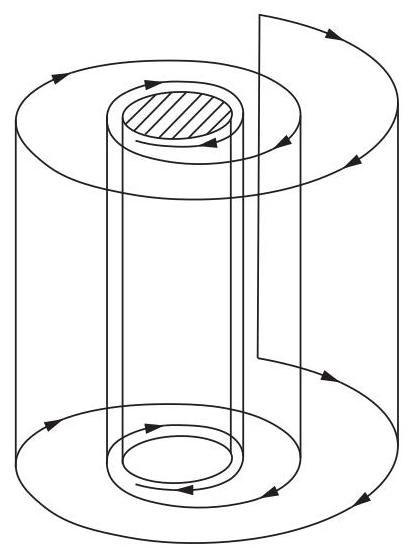
\includegraphics[max width=0.3\textwidth]{images/bo_d4b9jf3ef24c73e0334g_349_309_190_408_548_0.jpg}
\end{center}
\hspace*{3em} 

图 5-7.一个完备的非闭合曲面.

\begin{center}
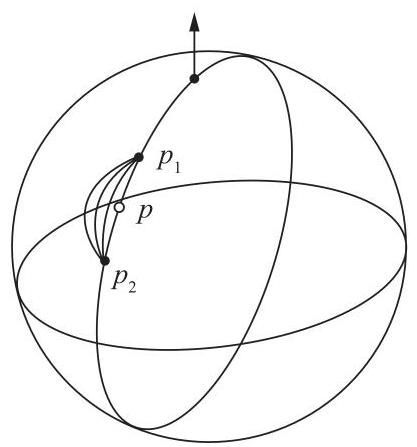
\includegraphics[max width=0.3\textwidth]{images/bo_d4b9jf3ef24c73e0334g_349_935_291_417_447_0.jpg}
\end{center}
\hspace*{3em} 

图 5-8

注意到极小测地线可能不存在，如下例所示.

设 \({S}^{2} - \{ p\}\) 是由球面 \({S}^{2}\) 减去点 \(p \in  {S}^{2}\) 形成的曲面.通过在通过 \(p\) 的经线上取两个点 \({p}_{1}\) 和 \({p}_{2}\) ，它们相对于 \(p\) 对称且足够接近 \(p\) ，我们发现曲面 \({S}^{2} - \{ p\}\) 上不存在连接 \({p}_{1}\) 和 \({p}_{2}\) 的最小测地线(见图 5-8).

另一方面，曲面上两点之间可能存在无限多条最小测地线，例如球面上两个对径点的情况；连接这两个对径点的所有经线都是最小测地线.

本节的主要结果是，在一个完备曲面上，连接两给定点总存在一条最小测地线.

定理 1 (Hopf-Rinow).设 \(S\) 是一个完备曲面.给定两点 \(\mathrm{p},\mathrm{q} \in  S\) ，存在一条连接 \(\mathrm{p}\) 和 \(\mathrm{q}\) 的最小测地线.

证明.设 \(r = d\left( {p,q}\right)\) 是点 \(p\) 和 \(q\) 之间的距离.设 \({B}_{\delta }\left( 0\right)  \subset  {T}_{p}\left( S\right)\) 是一个半径为 \(\delta\) 的圆盘，以切平面 \({T}_{p}\left( S\right)\) 的原点 0 为中心，并包含在 0 的邻域 \(U \subset  {T}_{p}\left( S\right)\) 中，其中 \({\exp }_{p}\) 是一个微分同胚.设 \({B}_{\delta }\left( p\right)  = {\exp }_{p}\left( {{B}_{\delta }\left( 0\right) }\right)\) .注意到边界 Bd \({B}_{\delta }\left( p\right)  = \sum\) 是紧致的，因为它是紧致集 Bd \({B}_{\delta }\left( 0\right)  \subset  {T}_{p}\left( S\right) .\) 的连续像.

如果 \(x \in  \sum\) ，则连续函数 \(d\left( {x,q}\right)\) 在紧致集 \(\sum\) 的某点 \({x}_{0}\) 处达到最小值.点 \({x}_{0}\) 可以写成

\[
{x}_{0} = {\exp }_{p}\left( {\delta v}\right) ,\;\left| v\right|  = l,v \in  {T}_{p}\left( S\right) .
\]

\begin{center}
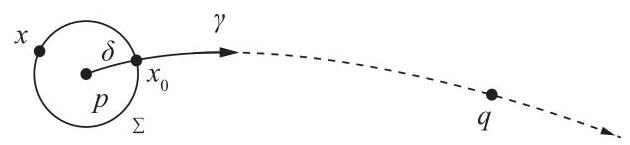
\includegraphics[max width=0.5\textwidth]{images/bo_d4b9jf3ef24c73e0334g_350_465_202_630_145_0.jpg}
\end{center}
\hspace*{3em} 

图 5-9

设 \(\gamma\) 是由弧长参数化的测地线，由(见图 5-9)给出

\[
\gamma \left( s\right)  = {\exp }_{p}\left( {sv}\right) .
\]

由于 \(S\) 是完备的， \(\gamma\) 对所有 \(s \in  R\) 都有定义.特别地， \(\gamma\) 在区间 \(\left\lbrack  {0,r}\right\rbrack\) 上有定义.如果我们证明 \(\gamma \left( r\right)  = q\) ，那么 \(\gamma\) 必须是一条连接 \(p\) 和 \(q\) 的测地线，并且是最小的，因为 \(l\left( \gamma \right)  = r = d\left( {p,q}\right)\) ，这将完成证明.

为了证明这一点，我们将证明，如果 \(s \in  \left\lbrack  {\delta ,r}\right\rbrack\) ，那么

\[
d\left( {\gamma \left( s\right) ,q}\right)  = r - s. \tag{1}
\]

方程 (1) 对 \(s = r\) 暗示 \(\gamma \left( r\right)  = q\) ，正如所期望的那样.

为证明式 (1)，我们首先证明它对 \(s = \delta\) 成立.现在集合 \(A = \{ s \in  \left\lbrack  {\delta ,r}\right\rbrack\) ；式 (1) 在 \(\}\) 中成立，该集合在 \(\left\lbrack  {0,r}\right\rbrack\) 中显然是闭合的.接下来我们证明，如果 \({s}_{0} \in  A\) 且 \({s}_{0} < r\) ，则式 (1) 对 \({S}_{0} + {\delta }^{\prime }\) 成立，其中 \({\delta }^{\prime } > 0\) 且 \({\delta }^{\prime }\) 足够小.由此得出 \(A = \left\lbrack  {\delta ,r}\right\rbrack\) ，式 (1) 得证.

我们现在证明式 (1) 对 \(s = \delta\) 成立.事实上，由于连接 \(p\) 到 \(q\) 的每条曲线都与 \(\sum\) 相交，我们有，令 \(x\) 为 \(\sum\) 的任意一点，

\[
d\left( {p,q}\right)  = \mathop{\inf }\limits_{\alpha }l\left( {\alpha }_{p,q}\right)  = \mathop{\inf }\limits_{{x \in  \sum }}\left\{  {\mathop{\inf }\limits_{\alpha }l\left( {\alpha }_{p,x}\right)  + \mathop{\inf }\limits_{\alpha }l\left( {\alpha }_{x,q}\right) }\right\}
\]

\[
= \mathop{\inf }\limits_{{x \in  \sum }}\left( {d\left( {p,x}\right)  + d\left( {x,q}\right) }\right)  = \mathop{\inf }\limits_{{x \in  \sum }}\left( {\delta  + d\left( {x,q}\right) }\right)
\]

\[
= \delta  + d\left( {{x}_{0},q}\right) .
\]

因此，

\[
d\left( {\gamma \left( \delta \right) ,q}\right)  = r - \delta ,
\]

即式 (1) 对 \(s = \delta\) 成立.

现在我们证明，如果式 (1) 对 \({s}_{0} \in  \left\lbrack  {\delta ,r}\right\rbrack\) 成立，那么对于 \({\delta }^{\prime } > 0\) 且足够小，它对 \({s}_{0} + {\delta }^{\prime }\) 成立.

设 \({B}_{{\delta }^{\prime }}\left( 0\right)\) 是切平面 \({T}_{\gamma \left( {s}_{0}\right) }\left( S\right)\) 中的一个圆盘，以该切平面的原点 0 为中心，并包含在邻域 \({U}^{\prime }\) 中，其中 \({\exp }_{\gamma \left( {s}_{0}\right) }\) 是一个微分同胚.设 \({B}_{{\delta }^{\prime }}\left( {\gamma \left( {s}_{0}\right) }\right)  = {\exp }_{\gamma \left( {s}_{0}\right) }{B}_{{\delta }^{\prime }}\left( 0\right)\) 且 \({\sum }^{\prime } = \operatorname{Bd}\left( {{B}_{{\delta }^{\prime }}\left( {\gamma \left( {s}_{0}\right) }\right) }\right.\) .如果 \({x}^{\prime } \in  {\sum }^{\prime }\) ，则连续函数 \(d\left( {{x}^{\prime },q}\right)\) 在 \({x}_{0}^{\prime } \in  {\sum }^{\prime }\) 处达到最小值(见图 5-10).那么，如前所述，

\[
d\left( {\gamma \left( {s}_{0}\right) ,q}\right)  = \mathop{\inf }\limits_{{{x}^{\prime } \in  {\sum }^{\prime }}}\left\{  {d\left( {\gamma \left( {s}_{0}\right) ,{x}^{\prime }}\right)  + d\left( {{x}^{\prime },q}\right) }\right\}
\]

\[
= {\delta }^{\prime } + d\left( {{x}_{0}^{\prime },q}\right) .
\]

\begin{center}
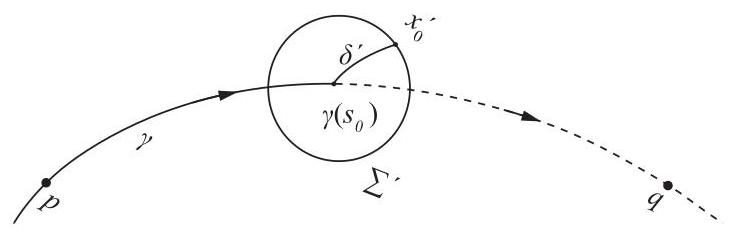
\includegraphics[max width=0.6\textwidth]{images/bo_d4b9jf3ef24c73e0334g_351_399_203_731_234_0.jpg}
\end{center}
\hspace*{3em} 

图 5-10

由于式 (1) 在 \({s}_{0}\) 中成立，我们有 \(d\left( {\gamma \left( {s}_{0}\right) ,q}\right)  = r - {s}_{0}\) .因此，

\[
d\left( {{x}_{0}^{\prime },q}\right)  = r - {s}_{0} - {\delta }^{\prime }. \tag{2}
\]

此外，由于

\[
d\left( {p,{x}_{0}^{\prime }}\right)  \geq  d\left( {p,q}\right)  - d\left( {q,{x}_{0}^{\prime }}\right) ,
\]

我们从式 (2) 得到

\[
d\left( {p,{x}_{0}^{\prime }}\right)  \geq  r - \left( {r - {s}_{0}}\right)  + {\delta }^{\prime } = {s}_{0} + {\delta }^{\prime }.
\]

现在观察从 \(p\) 到 \(\gamma \left( {s}_{0}\right)\) 经过 \(\gamma\) 的曲线，以及从 \(\gamma \left( {s}_{0}\right)\) 到 \({x}_{0}^{\prime }\) 经过半径为 \({B}_{{\delta }^{\prime }}\left( {\gamma \left( {s}_{0}\right) }\right)\) 的测地线段的曲线，其长度恰好等于 \({s}_{0} + {\delta }^{\prime }\) .由于 \(d\left( {p,{x}_{0}^{\prime }}\right)  \geq  {s}_{0} + {\delta }^{\prime }\) ，这条连接 \(p\) 到 \({x}_{0}^{\prime }\) 的曲线具有最小长度.由此可知(第 4-7 节，命题 2)，它是一条测地线，因此在其所有点上都是正则的.所以，它应该与 \(\gamma\) 重合；因此， \({x}_{0}^{\prime } = \gamma \left( {{s}_{0} + {\delta }^{\prime }}\right)\) .因此，方程 (2) 可以写成

\[
d\left( {\gamma \left( {{s}_{0} + {\delta }^{\prime }}\right) ,q}\right)  = r - \left( {{s}_{0} + {\delta }^{\prime }}\right) ,
\]

这是 \(s = {s}_{0} + {\delta }^{\prime }\) 的方程 (1).

这就证明了我们的论断并结束了证明.Q.E.D.

推论 1. 设 \(S\) 是完备的.则对于每一点 \(\mathrm{p} \in  S\) ，映射 \({\exp }_{\mathrm{p}} : {\mathrm{T}}_{\mathrm{p}}\left( S\right)  \rightarrow  S\) 是 \(S\) 上的满射.

这是正确的，因为如果 \(q \in  S\) 和 \(d\left( {p,q}\right)  = r\) ，那么 \(q = {\exp }_{p}{rv}\) ，其中 \(v = {\gamma }^{\prime }\left( 0\right)\) 是连接 \(p\) 到 \(q\) 的最小测地线 \(\gamma\) 的切向量，该测地线由弧长参数化.

推论 2. 设 \(S\) 是完备的且在度量 \(\mathrm{d}\) 中是有界的(即存在 \(\mathrm{r} > 0\) 使得对于任意一对 \(\mathrm{p},\mathrm{q} \in  S\) 都有 \(\mathrm{d}\left( {\mathrm{p},\mathrm{q}}\right)  < \mathrm{r}\) ).则 \(S\) 是紧致的.

证明.通过固定 \(p \in  S\) ， \(S\) 有界的事实意味着存在一个半径为 \(r\) 的闭球 \(B \subset  {T}_{p}\left( S\right)\) ，该球以切平面 \({T}_{p}\left( S\right)\) 的原点 0 为中心，使得 \({\exp }_{p}\left( B\right)  = {\exp }_{p}\left( {{T}_{p}\left( S\right) }\right)\) .根据 \({\exp }_{p}\) 是满射的事实，我们有 \(S = {\exp }_{p}\left( {{T}_{p}\left( S\right) }\right)  = {\exp }_{p}\left( B\right)\) .由于 \(B\) 是紧致的且 \({\exp }_{p}\) 是连续的，我们得出 \(S\) 是紧致的.Q.E.D.

从现在开始，除非另有说明，将要使用的度量概念将指定义 3 中的距离 \(d\) .例如，曲面 \(S\) 的直径 \(\rho \left( S\right)\) 定义为，

\[
\rho \left( s\right)  = \mathop{\sup }\limits_{{p,q \in  S}}d\left( {p,q}\right) .
\]

根据这个定义，单位球面 \({S}^{2}\) 的直径是 \(\rho \left( {S}^{2}\right)  = \pi\) .

\exerciseline

1. 设 \(S \subset  {R}^{3}\) 是一个完备曲面，设 \(F \subset  S\) 是 \(S\) 的一个非空闭子集，其补集 \(S - F\) 是连通的.证明 \(S - F\) 是一个非完备的正则曲面.

2. 令 \(S\) 为例 1 中的单叶锥.证明，给定 \(p \in  S\) ，在 \(S\) 上通过 \(p\) 且不能对参数的任意值进行延拓的唯一测地线是 \(S\) 上通过 \(p\) 的经线.

3. 令 \(S\) 为例 1 中的单叶锥.利用 4-2 节例 3 的等距性证明， \(S\) 上任意两点 \(p,q \in  S\) (见图 5-11)都可以通过一条最短测地线连接.

4. 我们称正则曲面 \(S \subset  {R}^{3}\) 上点列 \(\left\{  {p}_{n}\right\}\) 在(内禀)距离 \(d\) 下收敛于点 \({p}_{0} \in  S\) ，如果对于任意给定的 \(\epsilon  > 0\) ，存在一个指标 \({n}_{0}\) ，使得 \(n \geq  {n}_{0}\) 蕴含 \(d\left( {{p}_{n},{p}_{0}}\right)  > \epsilon\) .证明点列 \(\left\{  {p}_{n}\right\}\) 在 \(S\) 中在 \(d\) 下收敛于 \({p}_{0} \in  S\) 当且仅当 \(\left\{  {p}_{n}\right\}\) 作为 \({R}^{3}\) 中的点列(即在欧氏距离下)收敛于 \({p}_{0}\) .

\begin{center}
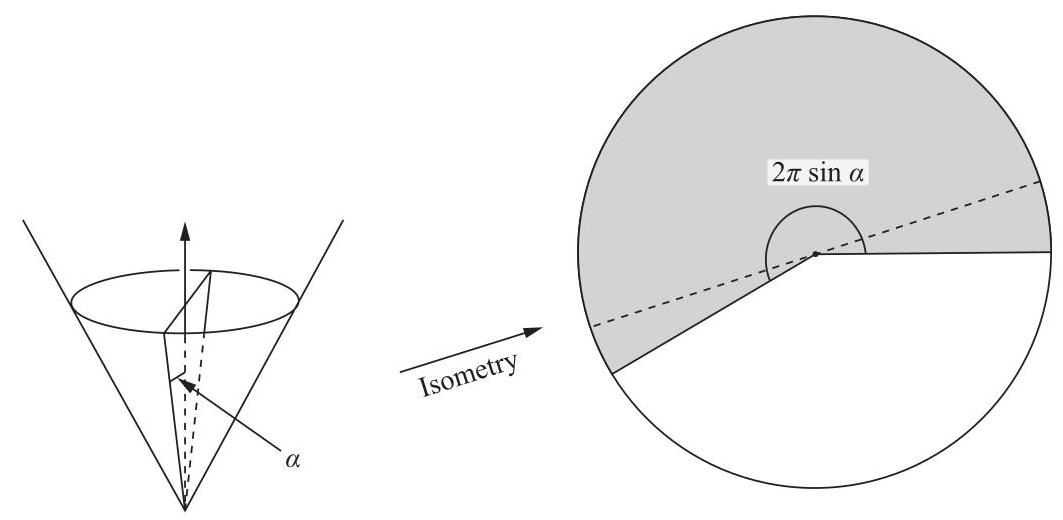
\includegraphics[max width=0.9\textwidth]{images/bo_d4b9jf3ef24c73e0334g_352_246_1521_1063_520_0.jpg}
\end{center}
\hspace*{3em} 

图 5-11

*5. 令 \(S \subset  {R}^{3}\) 为一个正则曲面.曲面 \(S\) 上的点列 \(\left\{  {p}_{n}\right\}\) 在(内禀)距离 \(d\) 下是柯西序列，如果对于任意给定的 \(\epsilon  > 0\) ，存在一个指标 \({n}_{0}\) ，使得当 \(n,m \geq  {n}_{0}\) 时，则 \(d\left( {{p}_{n},{p}_{m}}\right)  < \epsilon\) .证明 \(S\) 是完备的当且仅当 \(S\) 上的每个柯西序列都收敛于 \(S\) 中的一个点.

*6. 曲面 \(S\) 上的测地线 \(\gamma  : \lbrack 0,\infty ) \rightarrow  S\) 是从 \(\gamma \left( 0\right)\) 发出的射线，如果它对所有 \(s \in  \lbrack 0,\infty )\) 都实现了 \(\gamma \left( 0\right)\) 和 \(\gamma \left( s\right)\) 之间的(内禀)距离.令 \(p\) 为完备、非紧曲面 \(S\) 上的一点.证明 \(S\) 包含一条从 \(p\) 发出的射线.

7. \(S\) 上的发散曲线是一个可微映射 \(\alpha  : \lbrack 0,\infty ) \rightarrow  S\) ，使得对于每个紧子集 \(K \subset  S\) ，存在一个 \({t}_{0} \in  \left( {0,\infty }\right)\) ，使得对于 \(t > {t}_{0}\) 有 \(\alpha \left( t\right)  \notin  K\) (即 \(\alpha\) “离开” \(S\) 的每个紧子集).发散曲线的长度定义为

\[
\mathop{\lim }\limits_{{t \rightarrow  \infty }}{\int }_{0}^{t}\left| {{\alpha }^{\prime }\left( t\right) }\right| {dt}
\]

证明 \(S \subset  {R}^{3}\) 是完备的当且仅当每条发散曲线的长度是无界的.

*8. 令 \(S\) 和 \(\bar{S}\) 为正则曲面，令 \(\varphi  : S \rightarrow  \bar{S}\) 为一个微分同胚.假设 \(\bar{S}\) 是完备的，并且存在一个常数 \(c > 0\) 使得

\[
{I}_{p}\left( v\right)  \geq  c{\bar{I}}_{\varphi \left( p\right) }\left( {d{\varphi }_{p}\left( v\right) }\right)
\]

对于所有 \(p \in  S\) 和所有 \(v \in  {T}_{p}\left( S\right)\) ，其中 \(I\) 和 \(\bar{I}\) 分别表示 \(S\) 和 \(\bar{S}\) 的第一基本形式.证明 \(S\) 是完备的.

*9. 设 \({S}_{1} \subset  {R}^{3}\) 为一个(连通的)完备曲面，设 \({S}_{2} \subset  {R}^{3}\) 为一个连通曲面，使得 \({S}_{2}\) 的任意两点都可以由一条唯一的测地线连接.设 \(\varphi  : {S}_{1} \rightarrow  {S}_{2}\) 为一个局部等距映射.证明 \(\varphi\) 是一个全局等距映射.

*10. 设 \(S \in  {R}^{3}\) 为一个完备曲面.固定一个单位向量 \(v \in  {R}^{3}\) ，设 \(h : S \rightarrow \; R\) 为高度函数 \(h\left( p\right)  = \langle p,v\rangle ,p \in  S\) .我们回顾 \(h\) 的梯度是 \(S\) 上的(切)向量场 grad \(h\) ，定义为

\[
\langle \operatorname{grad}h\left( p\right) ,w{\rangle }_{p} = d{h}_{p}\left( w\right) \;\text{ for all }w \in  {T}_{p}\left( S\right)
\]

(参见练习 14，第 2-5 节).设 \(\alpha \left( t\right)\) 为 grad \(h\) 的一条轨迹；即， \(\alpha \left( t\right)\) 是 \(S\) 上的一个曲线，使得 \({\alpha }^{\prime }\left( t\right)  = \operatorname{grad}h\left( {\alpha \left( t\right) }\right)\) .证明

a. 对所有 \(p \in  S\) ， \(\left| {\operatorname{grad}h\left( p\right) }\right|  \leq  1\) 成立.

b. grad \(h\) 的一条轨迹 \(\alpha \left( t\right)\) 对所有 \(t \in  R\) 都有定义.

以下练习假定已掌握第 3-5 节 B 部分的材料以及复变函数的基本知识.

11. (Osserman 引理.) 设 \({D}_{1} = \{ \zeta  \in  \mathbb{C};\left| \zeta \right|  \leq  1\}\) 为复平面 \(\mathbb{C}\) 中的单位圆盘.照常，我们通过 \(\zeta  = u + {iv}\) 来识别 \(\mathbb{C} \approx  {R}^{2}\) .设 \(\mathbf{x} : {D}_{1} \rightarrow  {R}^{3}\) 是一个极小曲面 \(\mathbf{x}\left( {D}_{1}\right)  \subset  {R}^{3}\) 的等温参数化.这意味着(参见第 3-5 节 B 部分)

\[
\left\langle  {{\mathbf{x}}_{u},{\mathbf{x}}_{u}}\right\rangle   = \left\langle  {{\mathbf{x}}_{v},{\mathbf{x}}_{v}}\right\rangle  ,\;\left\langle  {{\mathbf{x}}_{u},{\mathbf{x}}_{v}}\right\rangle   = 0
\]

以及(极小性条件)

\[
{\mathbf{x}}_{uu} + {\mathbf{x}}_{vv} = 0.
\]

假设 \(\mathbf{x}\left( {D}_{1}\right)\) 的单位法向量避开了单位球的某个邻域.更确切地说，假设对于某个向量 \(w \in  {R}^{3}\) ， \(\left| w\right|  = 1\) ，存在一个 \(\epsilon  > 0\) 使得

\[
\frac{{\left\langle  {\mathbf{x}}_{u},w\right\rangle  }^{2}}{{\left| {\mathbf{x}}_{u}\right| }^{2}} \geq  {\epsilon }^{2}\;\text{ and }\;\frac{{\left\langle  {\mathbf{x}}_{v},w\right\rangle  }^{2}}{{\left| {\mathbf{x}}_{v}\right| }^{2}} \geq  {\epsilon }^{2}.
\]
 (*)

本练习的目标是证明 \(\mathbf{x}\left( D\right)\) 不是一个完备曲面.(这是第 3-5 节末尾引用的 Osserman 定理证明中的关键步骤.)按以下步骤进行:

a. 定义 \(\varphi  : {D}_{1} \rightarrow  \mathbb{C}\) 为

\[
\varphi \left( {u,v}\right)  = \varphi \left( \zeta \right)  = \left\langle  {{\mathbf{x}}_{\mathbf{u}},w}\right\rangle   + i\left\langle  {{\mathbf{x}}_{v},w}\right\rangle  .
\]

证明极小性条件意味着 \(\varphi\) 是解析的.

b. 定义 \(\theta  : {D}_{1} \rightarrow  \mathbb{C}\) 为

\[
\theta \left( \zeta \right)  = {\int }_{0}^{\zeta }\varphi \left( \zeta \right) {d\zeta } = \eta .
\]

根据 a 部分， \(\theta\) 是一个解析函数.证明 \(\theta \left( 0\right)  = 0\) 成立，并且条件 \(\left( *\right)\) 意味着 \({\theta }^{\prime }\left( \zeta \right)  \neq  0\) .因此，在 0 的某个邻域内， \(\theta\) 有一个解析逆函数 \({\theta }^{-1}\) .使用 Liouville 定理证明 \({\theta }^{-1}\) 不能解析地延拓到整个 \(\mathbb{C}\) .

c. 根据 b 部分，存在一个圆盘

\[
{D}_{R} = \{ \eta  \in  \mathbb{C};\left| \eta \right|  \leq  R\}
\]

以及一个点 \({\eta }_{0}\) ，其中 \(\left| {\eta }_{0}\right|  = R\) ，使得 \({\theta }^{-1}\) 在 \(D\) 中是解析的，并且不能解析地延拓到 \({\eta }_{0}\) 的某个邻域(图 5-12).

\begin{center}
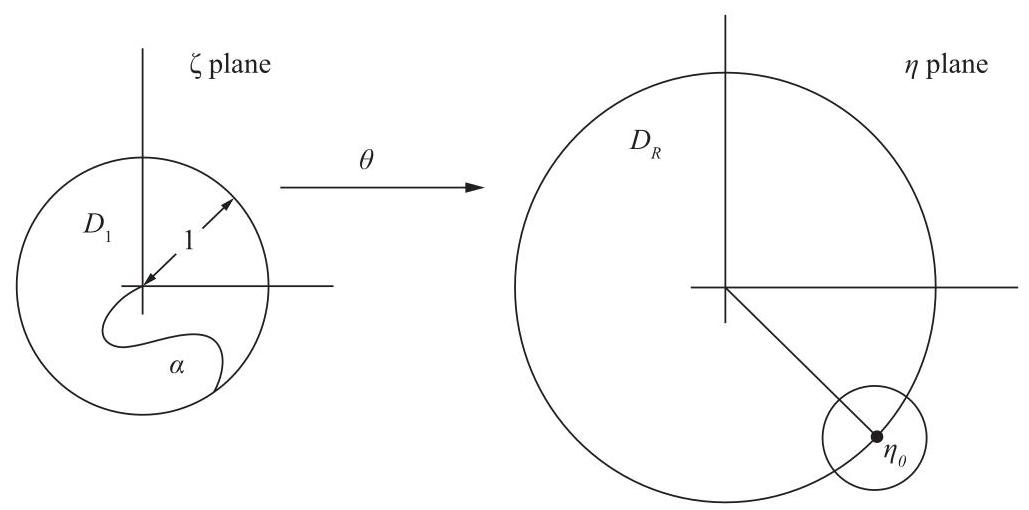
\includegraphics[max width=0.9\textwidth]{images/bo_d4b9jf3ef24c73e0334g_355_250_191_1029_510_0.jpg}
\end{center}
\hspace*{3em} 

图 5-12

设 \(L\) 为连接 \({\eta }_{0}\) 和 0 的 \({D}_{R}\) 的一段；即， \(L = \left\{  {t{\eta }_{0} \in  \mathbb{C};0 \leq  }\right. \; t \leq  1\}\) .令 \(\alpha  = {\theta }^{-1}\left( L\right)\) 并证明 \(\mathbf{x}\left( \alpha \right)\) 的弧长 \(l\) 为

\[
l = {\int }_{\alpha }\sqrt{2\left\langle  {{\mathbf{x}}_{u},{\mathbf{x}}_{v}}\right\rangle  \left\{  {{\left( \frac{du}{dt}\right) }^{2} + {\left( \frac{dv}{dt}\right) }^{2}}\right\}  }{dt}
\]

\[
\leq  \frac{1}{\epsilon }{\int }_{\alpha }\sqrt{{\left\langle  {\mathbf{x}}_{u},w\right\rangle  }^{2} + {\left\langle  {\mathbf{x}}_{v},w\right\rangle  }^{2}}\left| {d\zeta }\right|  = \frac{1}{\epsilon }{\int }_{\alpha }\left| {\varphi \left( \zeta \right) }\right| \left| {d\zeta }\right|
\]

\[
= \frac{R}{\epsilon } <  + \infty \text{ . }
\]

利用练习 7 得出 \(\mathbf{x}\left( D\right)\) 不完整.

\section*{5-4. 弧长的一阶和二阶变分；Bonnet 定理}

本节的目标是证明一个具有高斯曲率 \(S\) 的完整曲面 \(K \geq  \delta  > 0\) 是紧致的(Bonnet 定理).

证明的关键在于表明，如果 \(K \geq  \delta  > 0\) 是连接任意两点 \(\gamma\) 和 \(p,q \in  S\) 且长度为 \(l\left( \gamma \right)  > \pi /\sqrt{\delta }\) 的测地线，那么它不再是极小值；也就是说，存在一条连接 \(p\) 和 \(q\) 的参数化曲线，其长度小于 \(l\left( \gamma \right)\) .

一旦证明了这一点，就可以得出每条极小测地线的长度为 \(l \leq  \pi /\sqrt{\delta }\) ；因此， \(S\) 在距离 \(d\) 上是有界的.由于 \(S\) 是完整的， \(S\) 是紧致的(第 5-3 节推论 2).我们注意到，此外，我们还得到了 \(S\) 直径的估计值，即 \(\rho \left( S\right)  \leq  \pi /\sqrt{\delta }\) .

为了证明上述观点，我们需要将参数化曲线的弧长与“邻近曲线”的弧长进行比较.为此，我们将引入一些在微分几何的其他问题中有用的概念.实际上，这些概念是对变分学中更一般概念的微分几何适应.不假设任何变分学知识.

在本节中， \(S\) 表示一个正则(不一定是完整的)曲面.

我们将首先精确化给定曲线的邻近曲线的概念.

定义 1. 令 \(\alpha  : \left\lbrack  {0,l}\right\rbrack   \rightarrow  S\) 为一条正则参数化曲线，其中参数 \(S \in  \left\lbrack  {0,l}\right\rbrack\) 为弧长. \(\alpha\) 的一个变分是一个可微映射 \(\mathrm{h} : \left\lbrack  {0,l}\right\rbrack   \times  \left( {-\epsilon ,\epsilon }\right)  \subset  {\mathbb{R}}^{2} \rightarrow  S\) ，使得

\[
\mathrm{h}\left( {S,0}\right)  = \alpha \left( S\right) ,\;S \in  (0,l\rbrack .
\]

对于每个 \(\mathrm{t} \subset  \left( {-\epsilon ,\epsilon }\right)\) ，由 \({\mathrm{h}}_{\mathrm{t}} : \left\lbrack  {0,l}\right\rbrack   \rightarrow  S\) 给出的曲线 \({\mathrm{h}}_{\mathrm{t}}\left( s\right)  = \mathrm{h}\left( {S,\mathrm{t}}\right)\) 被称为变分 \(\mathrm{h}\) 的一条曲线.如果满足以下条件，则称变分 \(\mathrm{h}\) 为 proper:

\[
\mathrm{h}\left( {0,\mathrm{t}}\right)  = \alpha \left( 0\right) ,\;\mathrm{h}\left( {l,\mathrm{t}}\right)  = \alpha \left( l\right) ,\;\mathrm{t} \in  \left( {-\epsilon ,\epsilon }\right) .
\]

直观地说， \(\alpha\) 的一个变分是依赖于参数 \({h}_{t}\) 可微地变化的曲线族 \(t \in  \left( {-\epsilon ,\epsilon }\right)\) ，并且 \({h}_{0}\) 与 \(\alpha\) 一致(图 5-13).proper 的条件意味着所有曲线 \({h}_{t}\) 都具有相同的起点 \(\alpha \left( 0\right)\) 和相同的终点 \(\alpha \left( l\right)\) .

采用以下记法是方便的. \({R}^{2}\) 中的参数化曲线由以下方式给出:

\[
s \rightarrow  \left( {s,{t}_{0}}\right) ,
\]

\[
t \rightarrow  \left( {{s}_{0},t}\right)
\]

通过点 \({p}_{0} = \left( {{s}_{0},{t}_{0}}\right)  \in  {R}^{2}\) 且在 \(\left( {{s}_{0},{t}_{0}}\right)\) 处的切向量为 \(\left( {1,0}\right)\) 和 \(\left( {0,1}\right)\) .设 \(h : \left\lbrack  {0,l}\right\rbrack   \times  \left( {-\epsilon ,\epsilon }\right)  \subset  {R}^{2} \rightarrow  S\) 是一个可微映射，设 \({p}_{0} \in  \left\lbrack  {0,l}\right\rbrack   \times  \left( {-\epsilon ,\epsilon }\right)\) .则 \(d{h}_{{p}_{0}}\left( {1,0}\right)\) 是曲线 \(s \rightarrow  h\left( {s,{t}_{0}}\right)\) 在 \(h\left( {p}_{0}\right)\) 处的切向量，而 \(d{h}_{{p}_{0}}\left( {0,1}\right)\) 是曲线 \(t \rightarrow  h\left( {{s}_{0},t}\right)\) 在 \(h\left( {p}_{0}\right)\) 处的切向量.我们将记作

\[
d{h}_{{p}_{0}}\left( {1,0}\right)  = \frac{\partial h}{\partial s}\left( {p}_{0}\right) ,
\]

\[
d{h}_{{p}_{0}}\left( {0,1}\right)  = \frac{\partial h}{\partial t}\left( {p}_{0}\right) .
\]

\begin{center}
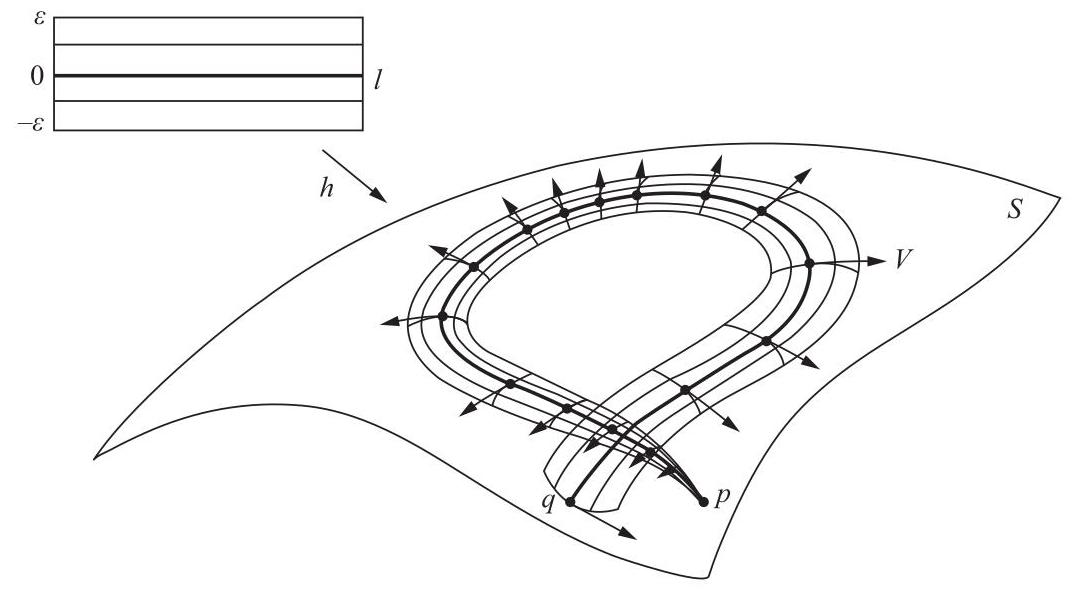
\includegraphics[max width=0.9\textwidth]{images/bo_d4b9jf3ef24c73e0334g_356_243_1454_1077_590_0.jpg}
\end{center}
\hspace*{3em} 

图 5-13

我们回顾(参见第 4-4 节，定义 3)沿曲线 \(\alpha  : I \rightarrow  S\) 的向量场 \(w\) 是一个对应关系，它将每个 \(t \in  I\) 分配给一个切于曲面 \(S\) 在 \(\alpha \left( t\right)\) 处的向量 \(w\left( t\right)\) .因此， \(\partial h/\partial s\) 和 \(\partial h/\partial t\) 是沿 \(\alpha\) 的可微切向量场.

由此可知， \(\alpha\) 的一个变分 \(h\) 通过以下方式确定一个沿 \(\alpha\) 的可微向量场 \(V\left( s\right)\) :

\[
V\left( s\right)  = \frac{\partial h}{\partial t}\left( {s,0}\right) ,\;S \in  \left\lbrack  {0,l}\right\rbrack  .
\]

\(V\) 称为 \(h\) 的变分向量场；我们注意到，如果 \(h\) 是 proper 的，则

\[
V\left( 0\right)  = V\left( l\right)  = 0
\]

以下命题证明了这种术语的合理性.

命题 1. 如果设 V(s) 是参数化正则曲线 \(\alpha  : \left\lbrack  {0,l}\right\rbrack   \rightarrow  S\) 沿的某个可微向量场，则存在 \(\alpha\) 的一个变分 \(\mathrm{h} : \left\lbrack  {0,l}\right\rbrack   \times  \left( {-\epsilon ,\epsilon }\right)  \rightarrow  S\) ，使得 \(\mathrm{V}\left( S\right)\) 是 \(\mathrm{h}\) 的变分向量场.此外，如果 \(\mathrm{V}\left( 0\right)  = \mathrm{V}\left( l\right)  = 0\) ，则 \(\mathrm{h}\) 可以选择为 proper 的.

证明.我们首先证明存在一个 \(\delta  > 0\) ，使得如果 \(\left| v\right|  < \delta\) ， \(v \in  {T}_{\alpha \left( s\right) }\left( S\right)\) ，则对于所有 \(s \in  \left\lbrack  {0,l}\right\rbrack\) ， \({\exp }_{\alpha \left( s\right) }v\) 是良定义的.事实上，对于每个 \(p \in  \alpha \left( \left\lbrack  {0,l}\right\rbrack  \right)  \subset  S\) ，考虑邻域 \({W}_{p}\) (它是其所有点的正常邻域)以及由第 4-7 节的命题 1 给出的数 \({\delta }_{p} > 0\) .并集 \(\mathop{\bigcup }\limits_{p}{W}_{p}\) 覆盖 \(\alpha \left( \left\lbrack  {0,l}\right\rbrack  \right)\) ，并且由于紧致性，其中有限个，例如 \({W}_{1},\ldots ,{W}_{n}\) ，仍然覆盖 \(\alpha \left( \left\lbrack  {0,l}\right\rbrack  \right)\) .令 \(\delta  = \min \left( {{\delta }_{1},\ldots ,{\delta }_{n}}\right)\) ，其中 \({\delta }_{i}\) 是与邻域 \({W}_{i},i = 1,\ldots ,n\) 对应的数.很容易看出 \(\delta\) 满足上述条件.

现在令 \(M = \mathop{\max }\limits_{{s \in  \left\lbrack  {0,l}\right\rbrack  }}\left| {V\left( s\right) }\right| ,\epsilon  < \delta /M\) ，并定义

\[
h\left( {s,t}\right)  = {\exp }_{\alpha \left( t\right) }{tV}\left( s\right) ,\;s \in  \left\lbrack  {0,l}\right\rbrack  ,\;t \in  \left( {-\epsilon ,\epsilon }\right) .
\]

\(h\) 是良定义的，这很明显.此外，由于

\[
\mathop{\exp }\limits_{{\alpha \left( s\right) }}{tV}\left( s\right)  = \gamma \left( {1,\alpha \left( s\right) ,{tV}\left( s\right) }\right) ,
\]

其中 \(\gamma\) 是第 4-7 节定理 1 的(可微)映射(即，对于 \(t \neq  0\) ，以及 \(V\left( s\right)  \neq  0,\gamma \left( {1,\alpha \left( s\right) ,{tV}\left( s\right) }\right)\) 是具有初始条件 \(\gamma \left( 0\right)  = \alpha \left( s\right) ,{\gamma }^{\prime }\left( 0\right)  = V\left( s\right) ),h\) 的测地线 \(\gamma\) 是可微的.可以立即检查出 \(h\left( {s,0}\right)  = \alpha \left( s\right)\) .最后， \(h\) 的变分向量场由下式给出

\[
\frac{\partial h}{\partial t}\left( {s,0}\right)  = d{h}_{\left( s,0\right) }\left( {0,1}\right)  = {\left. \frac{d}{dt}\left( {\exp }_{\alpha \left( s\right) }tV\left( s\right) \right) \right| }_{t = 0}
\]

\[
= {\left. \frac{d}{dt}\gamma \left( 1,\alpha \left( s\right) ,tV\left( s\right) \right) \right| }_{t = 0} = {\left. \frac{d}{dt}\gamma \left( t,\alpha \left( s\right) ,V\left( s\right) \right) \right| }_{t = 0} = V\left( s\right) ,
\]

并且根据 \(h\) 的定义，很明显，如果 \(V\left( 0\right)  = V\left( l\right)  = 0\) ，则 \(h\) 是真子集.

Q.E.D.

我们想比较 \(\alpha \left( { = {h}_{0}}\right)\) 的弧长与 \({h}_{t}\) 的弧长.因此，我们定义一个函数 \(L : \left( {-\epsilon ,\epsilon }\right)  \rightarrow  R\) 如下:

\[
L\left( t\right)  = {\int }_{0}^{l}\left| {\frac{\partial h}{\partial s}\left( {s,t}\right) }\right| {ds},\;t \in  \left( {-\epsilon ,\epsilon }\right) . \tag{1}
\]

对 \(L\) 在 \(t = 0\) 的邻域中的研究将告知我们邻近 \(\alpha\) 的曲线的“弧长行为”.

我们需要一些预备引理.

引理 1. 由方程 (1) 定义的函数 L 在 \(\mathrm{t} = 0\) 的邻域中是可微的；在该邻域中，可以通过在积分号下微分来获得 \(\mathrm{L}\) 的导数.

证明.由于 \(\alpha  : \left\lbrack  {0,l}\right\rbrack   \rightarrow  S\) 是由弧长参数化的，

\[
\left| \frac{\partial h}{\partial s}\right|  = \left| {\frac{\partial h}{\partial s}\left( {s,0}\right) }\right|  = 1.
\]

因此，由于 \(\left\lbrack  {0,l}\right\rbrack\) 的紧致性，存在一个 \(\delta  > 0,\delta  \leq  \epsilon\) ，使得

\[
\left| {\frac{\partial h}{\partial s}\left( {s,t}\right) }\right|  \neq  0,\;s \in  \left\lbrack  {0,l}\right\rbrack  ,\;\left| t\right|  < \delta .
\]

由于非零可微函数的绝对值是可微的，因此式 (1) 的被积函数在 \(\left| t\right|  < \delta\) 上是可微的.根据微积分的一个经典定理(参见 R. C. Buck, Advanced Calculus, 1965, p. 120)，我们得出结论: \(L\) 在 \(\left| t\right|  < \delta\) 上是可微的，并且

\[
{L}^{\prime }\left( t\right)  = {\int }_{0}^{l}\frac{\partial }{\partial t}\left| {\frac{\partial h}{\partial s}\left( {s,t}\right) }\right| {ds}. \tag{Q.E.D.}
\]

下文的引理 2、3 和 4 具有一定的独立意义.

引理 2. 设 \(\mathrm{w}\left( \mathrm{t}\right)\) 是沿参数化曲线 \(\alpha  : \left\lbrack  {\mathrm{a},\mathrm{b}}\right\rbrack   \rightarrow  S\) 的可微向量场，设 \(\mathrm{f} : \left\lbrack  {\mathrm{a},\mathrm{b}}\right\rbrack   \rightarrow  \mathbb{R}\) 是一个可微函数.则

\[
\frac{\mathrm{D}}{\mathrm{{dt}}}\left( {\mathrm{f}\left( \mathrm{t}\right) \mathrm{w}\left( \mathrm{t}\right) }\right)  = \mathrm{f}\left( \mathrm{t}\right) \frac{\mathrm{{DW}}}{\mathrm{{dt}}} + \frac{\mathrm{{df}}}{\mathrm{{dt}}}\mathrm{w}\left( \mathrm{t}\right) .
\]

证明. 仅需使用协变导数是通常导数的切向分量的这一事实，即可得出(此处 \({\left( \right) }_{T}\) 表示 \(\left( \;\right) )\) 的切向分量)

\[
\frac{D}{dt}\left( {fw}\right)  = {\left( \frac{df}{dt}w + f\frac{dw}{dt}\right) }_{T} = \frac{df}{dt}w + f{\left( \frac{dw}{dt}\right) }_{T}
\]

\[
= \frac{df}{dt}w + f\frac{Dw}{dt}. \tag{Q.E.D.}
\]

引理 3. 设 \(\mathrm{v}\left( \mathrm{t}\right)\) 和 \(\mathrm{w}\left( \mathrm{t}\right)\) 是沿参数化曲线 \(\alpha  : \left\lbrack  {\mathrm{a},\mathrm{b}}\right\rbrack   \rightarrow  S\) 的可微向量场.则

\[
\frac{\mathrm{d}}{\mathrm{{dt}}}\langle \mathrm{v}\left( \mathrm{t}\right) ,\mathrm{w}\left( \mathrm{t}\right) \rangle  = \left\langle  {\frac{\mathrm{{DV}}}{\mathrm{{dt}}},\mathrm{w}\left( \mathrm{t}\right) }\right\rangle   + \left\langle  {\mathrm{v}\left( \mathrm{t}\right) ,\frac{\mathrm{{DW}}}{\mathrm{{dt}}}}\right\rangle  .
\]

证明. 利用上述证明中的说明，我们得到

\[
\frac{d}{dt}\langle v,w\rangle  = \left\langle  {\frac{dv}{dt},w}\right\rangle   + \left\langle  {v,\frac{dw}{dt}}\right\rangle   = \left\langle  {{\left( \frac{dv}{dt}\right) }_{T},w}\right\rangle   + \left\langle  {v,{\left( \frac{dw}{dt}\right) }_{T}}\right\rangle
\]

\[
= \left\langle  {\frac{Dv}{dt},w}\right\rangle   + \left\langle  {v,\frac{Dw}{dt}}\right\rangle  . \tag{Q.E.D.}
\]

在陈述下一个引理之前，引入以下术语是方便的.设 \(h : \left\lbrack  {0,l}\right\rbrack   \times  \left( {-\epsilon ,\epsilon }\right)  \rightarrow  S\) 是一个可微映射.沿 \(h\) 的可微向量场 \(A\) 是一个可微映射

\[
V : \left\lbrack  {0,l}\right\rbrack   \times  \left( {-\epsilon ,\epsilon }\right)  \rightarrow  T\left( S\right)  \subset  {R}^{3}
\]

使得对于每一个 \(\left( {s,t}\right)  \in  \left\lbrack  {0,l}\right\rbrack   \times  \left( {-\epsilon ,\epsilon }\right)\) 都存在 \(V\left( {s,t}\right)  \in  {T}_{h\left( {s,t}\right) }\left( S\right)\) .这推广了可微向量场沿参数化曲线的定义(第 4-4 节，定义 2).

例如，上面引入的向量场 \(\left( {\partial h/\partial s}\right) \left( {s,t}\right)\) 和 \(\left( {\partial h/\partial t}\right) \left( {s,t}\right)\) 是沿 \(h\) 的向量场.

如果我们限制 \(V\left( {s,t}\right)\) 到曲线 \(s =\) = const., \(t =\) = const.，我们得到沿曲线的向量场.在此上下文中，符号 \(\left( {{DV}/\partial t}\right) \left( {s,t}\right)\) 表示在点 \(\left( {s,t}\right)\) 处，对 \(V\left( {s,t}\right)\) 限制到曲线 \(s =\) = const. 的协变导数.

引理 4. 设 \(\mathrm{h} : \left\lbrack  {0,l}\right\rbrack   \times  \left( {-\epsilon ,\epsilon }\right)  \subset  {\mathbb{R}}^{2} \rightarrow  S\) 是一个可微映射.则

\[
\frac{\mathrm{D}}{\partial S}\frac{\partial \mathrm{h}}{\partial \mathrm{t}}\left( {S,\mathrm{t}}\right)  = \frac{\mathrm{D}}{\partial \mathrm{t}}\frac{\partial \mathrm{h}}{\partial S}\left( {S,\mathrm{t}}\right) .
\]

证明. 设 \(\mathbf{x} : U \rightarrow  S\) 是点 \(h\left( {s,t}\right)\) 处 \(S\) 的一个参数化，参数为 \(u,v\) ，并且设

\[
u = {h}_{1}\left( {s,t}\right) ,\;v = {h}_{2}\left( {s,t}\right)
\]

是 \(h\) 在此参数化下的表达式.在这些条件下，当 \(\left( {s,t}\right)  \in  {h}^{-1}\left( {\mathbf{x}\left( U\right) }\right)  = W\) 时，曲线 \(h\left( {s,{t}_{0}}\right)\) 可表示为

\[
u = {h}_{1}\left( {s,{t}_{0}}\right) ,\;v = {h}_{2}\left( {s,{t}_{0}}\right) .
\]

由于 \(\left( {\partial h/\partial s}\right) \left( {{s}_{0},{t}_{0}}\right)\) 在 \(s = {s}_{0}\) 处与曲线 \(h\left( {s,{t}_{0}}\right)\) 相切，我们得到

\[
\frac{\partial h}{\partial s}\left( {{s}_{0},{t}_{0}}\right)  = \frac{\partial {h}_{1}}{\partial s}\left( {{s}_{0},{t}_{0}}\right) {\mathbf{x}}_{u} + \frac{\partial {h}_{2}}{\partial s}\left( {{s}_{0},{t}_{0}}\right) {\mathbf{x}}_{v}.
\]

由于 \(\left( {{s}_{0},{t}_{0}}\right)  \in  W\) 的任意性，我们得出

\[
\frac{\partial h}{\partial s} = \frac{\partial {h}_{1}}{\partial s}{\mathbf{x}}_{u} + \frac{\partial {h}_{2}}{\partial s}{\mathbf{x}}_{v},
\]

为简化记法，此处省略了点 \(\left( {s,t}\right)\) 的指示.

同理，

\[
\frac{\partial h}{\partial t} = \frac{\partial {h}_{1}}{\partial t}{\mathbf{x}}_{u} + \frac{\partial {h}_{2}}{\partial t}{\mathbf{x}}_{v}.
\]

现在我们将使用协变导数用克里斯托费尔符号 \({\Gamma }_{ij}^{k}\) (第 4-4 节，公式 (1)) 表示的表达式来计算协变导数 \(\left( {D/\partial s}\right) \left( {\partial h/\partial t}\right)\) 和 \(\left( {D/\partial t}\right) \left( {\partial h/\partial s}\right)\) ，并得到所断言的等式.例如，两个导数中 \({\mathbf{x}}_{u}\) 的系数由下式给出:

\[
\frac{{\partial }^{2}{h}_{1}}{\partial s\partial t} + {\Gamma }_{11}^{1}\frac{\partial {h}_{1}}{\partial t}\frac{\partial {h}_{1}}{\partial s} + {\Gamma }_{12}^{1}\frac{\partial {h}_{1}}{\partial t}\frac{\partial {h}_{2}}{\partial s} + {\Gamma }_{12}^{1}\frac{\partial {h}_{2}}{\partial t}\frac{\partial {h}_{1}}{\partial s} + {\Gamma }_{22}^{1}\frac{\partial {h}_{2}}{\partial t}\frac{\partial {h}_{2}}{\partial s}.
\]

同理可证 \({\mathbf{x}}_{v}\) 的系数相等，从而完成证明.Q.E.D.

现在我们可以计算 \(L\) 在 \(t = 0\) 处的第一个导数，得到

命题 2. 设 \(\mathrm{h} : \left\lbrack  {0,l}\right\rbrack   \times  \left( {-\epsilon ,\epsilon }\right)\) 是曲线 \(\alpha  : \left\lbrack  {0,l}\right\rbrack   \rightarrow  S\) 的一个适当变分，设 \(\mathrm{V}\left( S\right)  = \left( {\partial \mathrm{h}/\partial \mathrm{t}}\right) \left( {S,0}\right) ,S \in  (0,l\rbrack\) 是 \(\mathrm{h}\) 的变分向量场.则

\[
{\mathrm{L}}^{\prime }\left( 0\right)  =  - {\int }_{0}^{l}\langle \mathrm{A}\left( S\right) ,\mathrm{V}\left( S\right) \rangle \mathrm{{ds}}, \tag{2}
\]

其中 \(\mathrm{A}\left( S\right)  = \left( {\mathrm{D}/\partial S}\right) \left( {\partial \mathrm{h}/\partial S}\right) \left( {S,0}\right)\) .

证明. 如果 \(t\) 属于引理 1 给出的区间 \(\left( {-\delta ,\delta }\right)\) ，则

\[
{L}^{\prime }\left( t\right)  = {\int }_{0}^{l}\left\{  {\frac{d}{dt}{\left\langle  \frac{\partial h}{\partial s},\frac{\partial h}{\partial s}\right\rangle  }^{1/2}}\right\}  {ds}.
\]

应用引理 3 和 4，我们得到

\[
{L}^{\prime }\left( t\right)  = {\int }_{l}^{0}\frac{\left\langle  \frac{D}{\partial t}\frac{\partial h}{\partial s},\frac{\partial h}{\partial s}\right\rangle  }{\left| \frac{\partial h}{\partial s}\right| }{ds} = {\int }_{0}^{l}\frac{\left\langle  \frac{D}{\partial s}\frac{\partial h}{\partial t},\frac{\partial h}{\partial s}\right\rangle  }{\left| \frac{\partial h}{\partial s}\right| }{ds}.
\]

由于 \(\left| {\left( {\partial h/\partial s}\right) \left( {s,0}\right) }\right|  = 1\) ，我们得到

\[
{L}^{\prime }\left( 0\right)  = {\int }_{0}^{l}\left\langle  {\frac{D}{\partial s}\frac{\partial h}{\partial t},\frac{\partial h}{\partial s}}\right\rangle  {ds},
\]

其中被积函数在 \(\left( {s,0}\right)\) 处计算，为简化记法省略了.

根据引理 3，

\[
\frac{\partial }{\partial s}\left\langle  {\frac{\partial h}{\partial s},\frac{\partial h}{\partial t}}\right\rangle   = \left\langle  {\frac{D}{\partial s}\frac{\partial h}{\partial s},\frac{\partial h}{\partial t}}\right\rangle   + \left\langle  {\frac{\partial h}{\partial s},\frac{D}{\partial s}\frac{\partial h}{\partial t}}\right\rangle  .
\]

因此，

\[
{L}^{\prime }\left( 0\right)  = {\int }_{0}^{l}\frac{\partial }{\partial s}\left\langle  {\frac{\partial h}{\partial s},\frac{\partial h}{\partial t}}\right\rangle  {ds} - {\int }_{0}^{l}\left\langle  {\frac{D}{\partial s}\frac{\partial h}{\partial s},\frac{\partial h}{\partial t}}\right\rangle  {ds}
\]

\[
=  - {\int }_{0}^{l}\left\langle  {\frac{D}{\partial s}\frac{\partial h}{\partial s},\frac{\partial h}{\partial t}}\right\rangle  {ds},
\]

由于 \(\left( {\partial h/\partial t}\right) \left( {0,0}\right)  = \left( {\partial h/\partial t}\right) \left( {l,0}\right)  = 0\) ，这是因为变分是适当的.回想 \(A\left( s\right)\) 和 \(V\left( s\right)\) 的定义，我们可以将最后一个表达式写成

\[
{L}^{\prime }\left( 0\right)  =  - {\int }_{0}^{l}\langle A\left( s\right) ,V\left( s\right) \rangle {ds}. \tag{Q.E.D.}
\]

注1. 向量 \(A\left( s\right)\) 称为曲线 \(\alpha\) 的加速度向量，其范数即为 \(\alpha\) 的测地曲率的绝对值.注意到 \({L}^{\prime }\left( 0\right)\) 仅取决于变分场 \(V\left( s\right)\) 而非变分 \(h\) 本身.式(2)通常称为曲线 \(\alpha\) 的弧长的一阶变分公式.

注2. \(h\) 是合适的条件仅在证明的最后用于消除项

\[
\left\langle  {\frac{\partial h}{\partial s},\frac{\partial h}{\partial t}}\right\rangle  \left( {l,0}\right)  - \left\langle  {\frac{\partial h}{\partial s},\frac{\partial h}{\partial t}}\right\rangle  \left( {0,0}\right) .
\]

因此，如果 \(h\) 不合适，我们将得到一个类似于式(2)的公式，其中包含这些额外的边界项.

命题2的一个有趣推论是将测地线刻画为“变分问题”的解.更精确地说，

命题3. 正则参数化曲线 \(\alpha  : \left\lbrack  {0,l}\right\rbrack   \rightarrow  S\) ，其中参数 \(S \in  \left\lbrack  {0,l}\right\rbrack\) 是 \(\alpha\) 的弧长，是测地线当且仅当对于 \(\alpha ,{\mathrm{L}}^{\prime }\left( 0\right)  = 0\) 的每一次合适变分 \(\mathrm{h} : \left\lbrack  {0,l}\right\rbrack   \times  \left( {-\epsilon ,\epsilon }\right)  \rightarrow  S\) .

证明. 必要性是显然的，因为测地线 \(\alpha\) 的加速度向量 \(A\left( s\right)  = \; \left( {D/\partial s}\right) \left( {\partial \alpha /\partial s}\right)\) 恒为零.因此，对于每一次合适变分， \({L}^{\prime }\left( 0\right)  = 0\) .

现在假设对于 \(\alpha\) 的每一次合适变分都有 \({L}^{\prime }\left( 0\right)  = 0\) ，并考虑一个向量场 \(V\left( s\right)  = f\left( s\right) A\left( s\right)\) ，其中 \(f : \left\lbrack  {0,l}\right\rbrack   \rightarrow  R\) 是实可微函数，且 \(f\left( s\right)  \geq  0,f\left( 0\right)  = f\left( l\right)  = 0\) ，而 \(A\left( s\right)\) 是 \(\alpha\) 的加速度向量.通过构造一个对应于 \(V\left( s\right)\) 的变分，我们得到

\[
{L}^{\prime }\left( 0\right)  =  - {\int }_{0}^{l}\langle f\left( s\right) A\left( s\right) ,A\left( s\right) \rangle {ds}
\]

\[
=  - {\int }_{0}^{l}f\left( s\right) {\left| A\left( s\right) \right| }^{2}{ds} = 0.
\]

因此，由于 \(f\left( s\right) {\left| A\left( s\right) \right| }^{2} \geq  0\) ，我们得到

\[
f\left( s\right) {\left| A\left( s\right) \right| }^{2} \equiv  0.
\]

我们将证明上述关系蕴含 \(A\left( s\right)  = 0,s \in  \left\lbrack  {0,l}\right\rbrack\) .事实上，如果 \(\left| {A\left( {s}_{0}\right) }\right|  \neq  0,{s}_{0} \in  \left( {0,l}\right)\) ，则存在一个区间 \(I = \left( {{s}_{0} - \epsilon ,{s}_{0} + \epsilon }\right)\) 使得对于 \(s \in  I\) ，有 \(\left| {A\left( s\right) }\right|  \neq  0\) .通过选择 \(f\) 使得 \(f\left( {s}_{0}\right)  > 0\) ，我们与 \(f\left( {s}_{0}\right) \left| {A\left( {s}_{0}\right) }\right|  = 0\) 矛盾.因此，当 \(s \in  \left( {0,l}\right)\) 时， \(\left| {A\left( s\right) }\right|  = 0\) .由连续性可知， \(A\left( 0\right)  = A\left( l\right)  = 0\) ，正如所声称的.

由于 \(\alpha\) 的加速度矢量恒为零，因此 \(\alpha\) 是测地线.Q.E.D.

从现在开始，我们只考虑测地线 \(\gamma  : \left\lbrack  {0,l}\right\rbrack   \rightarrow  S\) 的真变分，由弧长参数化；也就是说，我们假设 \({L}^{\prime }\left( 0\right)  = 0\) .为了简化计算，我们将限制在正交变分；也就是说，我们假设变分场 \(V\left( s\right)\) 满足条件 \(\left\langle  {V\left( s\right) ,{\gamma }^{\prime }\left( s\right) }\right\rangle   = 0,s \in  \left\lbrack  {0,l}\right\rbrack\) .为了研究函数 \(L\) 在 0 的邻域中的行为，我们将计算 \({L}^{\prime \prime }\left( 0\right)\) .

对于这个计算，我们需要一些将高斯曲率与协变导数联系起来的引理.

引理 5. 令 \(x : \mathrm{U} \rightarrow  S\) 为正则曲面 \(S\) 在点 \(\mathrm{p} \in  S\) 的参数化，参数为 \(\mathrm{u},\mathrm{v}\) ，令 \(\mathrm{K}\) 为 S 的高斯曲率.则

\[
\frac{\mathrm{D}}{\partial \mathrm{v}}\frac{\mathrm{D}}{\partial \mathrm{u}}{\mathbf{x}}_{\mathrm{u}} - \frac{\mathrm{D}}{\partial \mathrm{u}}\frac{\mathrm{D}}{\partial \mathrm{v}}{\mathbf{x}}_{\mathrm{u}} = \mathrm{K}\left( {{\mathbf{x}}_{\mathrm{u}} \land  {\mathbf{x}}_{\mathrm{v}}}\right)  \land  {\mathbf{x}}_{\mathrm{u}}.
\]

证明. 通过观察到协变导数是切平面中通常导数的组成部分，我们得到(第 4-3 节)

\[
\frac{D}{\partial u}{\mathbf{x}}_{u} = {\Gamma }_{11}^{1}{\mathbf{x}}_{u} + {\Gamma }_{11}^{2}{\mathbf{x}}_{v}
\]

通过将协变导数的公式(第 4-4 节，方程 (1))应用于上述表达式，我们得到

\[
\frac{D}{\partial v}\left( {\frac{D}{\partial u}{\mathbf{x}}_{u}}\right)  = \left\{  {{\left( {\Gamma }_{11}^{1}\right) }_{v} + {\Gamma }_{12}^{1}{\Gamma }_{11}^{1} + {\Gamma }_{22}^{1}{\Gamma }_{11}^{2}}\right\}  {\mathbf{x}}_{u}
\]

\[
+ \left\{  {{\left( {\Gamma }_{11}^{2}\right) }_{v} + {\Gamma }_{12}^{2}{\Gamma }_{11}^{1} + {\Gamma }_{22}^{2}{\Gamma }_{11}^{2}}\right\}  {\mathbf{x}}_{v}.
\]

我们通过类似的计算验证

\[
\frac{D}{\partial u}\left( {\frac{D}{\partial v}{\mathbf{x}}_{u}}\right)  = \left\{  {{\left( {\Gamma }_{12}^{1}\right) }_{u} + {\Gamma }_{12}^{1}{\Gamma }_{11}^{1} + {\Gamma }_{12}^{1}{\Gamma }_{12}^{2}}\right\}  {\mathbf{x}}_{u}
\]

\[
+ \left\{  {{\left( {\Gamma }_{12}^{2}\right) }_{u} + {\Gamma }_{11}^{2}{\Gamma }_{12}^{1} + {\Gamma }_{12}^{2}{\Gamma }_{12}^{2}}\right\}  {\mathbf{x}}_{v}
\]

因此，

\[
\frac{D}{\partial v}\frac{D}{\partial u}{\mathbf{x}}_{u} - \frac{D}{\partial u}\frac{D}{\partial v}{\mathbf{x}}_{u} = \left\{  {{\left( {\Gamma }_{11}^{1}\right) }_{v} - {\left( {\Gamma }_{12}^{1}\right) }_{u} + {\Gamma }_{22}^{1}{\Gamma }_{11}^{2} - {\Gamma }_{12}^{1}{\Gamma }_{12}^{2}}\right\}  {\mathbf{x}}_{u}
\]

\[
+ \left\{  {{\left( {\Gamma }_{11}^{2}\right) }_{v} - {\left( {\Gamma }_{12}^{2}\right) }_{u} + {\Gamma }_{12}^{2}{\Gamma }_{11}^{1} + {\Gamma }_{22}^{2}{\Gamma }_{11}^{2}}\right.
\]

\[
\left. {-{\Gamma }_{11}^{2}{\Gamma }_{12}^{1} - {\Gamma }_{12}^{2}{\Gamma }_{12}^{2}}\right\}  {\mathbf{x}}_{v}.
\]

我们现在使用曲率用克里斯托费尔符号表示的表达式(第 4-3 节，方程 (5) 和 (5a))并得出结论

\[
\frac{D}{\partial v}\frac{D}{\partial u}{\mathbf{x}}_{u} - \frac{D}{\partial u}\frac{D}{\partial v}{\mathbf{x}}_{u} =  - {FK}{\mathbf{x}}_{u} + {EK}{\mathbf{x}}_{v}
\]

\[
= K\left\{  {\left\langle  {{\mathbf{x}}_{u},{\mathbf{x}}_{u}}\right\rangle  {\mathbf{x}}_{v} - \left\langle  {{\mathbf{x}}_{u},{\mathbf{x}}_{v}}\right\rangle  {\mathbf{x}}_{u}}\right\}
\]

\[
= K\left( {{\mathbf{x}}_{u} \land  {\mathbf{x}}_{v}}\right)  \land  {\mathbf{x}}_{u}. \tag{Q.E.D.}
\]

引理 6. 令 \(\mathrm{h} : \left\lbrack  {0,l}\right\rbrack   \times  \left( {-\epsilon ,\epsilon }\right)  \rightarrow  S\) 为一个可微映射，令 \(\mathrm{V}\left( {S,\mathrm{t}}\right) ,\left( {S,\mathrm{t}}\right)  \in  \left\lbrack  {0,l}\right\rbrack   \times  \left( {-\epsilon ,\epsilon }\right)\) 为 \(\mathrm{h}\) 沿的一个可微向量场.则

\[
\frac{\mathrm{D}}{\partial \mathrm{t}}\frac{\mathrm{D}}{\partial S}\mathrm{V} - \frac{\mathrm{D}}{\partial S}\frac{\mathrm{D}}{\partial \mathrm{t}}\mathrm{V} = \mathrm{K}\left( {S,\mathrm{t}}\right) \left( {\frac{\partial \mathrm{h}}{\partial S} \land  \frac{\partial \mathrm{h}}{\partial \mathrm{t}}}\right)  \land  \mathrm{V},
\]

其中 \(\mathrm{K}\left( {S,\mathrm{t}}\right)\) 是 \(S\) 在点 \(\mathrm{h}\left( {S,\mathrm{t}}\right)\) 的曲率.

证明. 令 \(\mathbf{x}\left( {u,v}\right)\) 为 \(S\) 在 \(h\left( {s,t}\right)\) 附近的坐标系，令

\[
V\left( {s,t}\right)  = a\left( {s,t}\right) {\mathbf{x}}_{u} + b\left( {s,t}\right) {\mathbf{x}}_{v}
\]

是该坐标系中 \(V\left( {s,t}\right)  = V\) 的表达式.根据引理 2，我们有

\[
\frac{D}{\partial s}V = \frac{D}{\partial s}\left( {a{\mathbf{x}}_{u} + b{\mathbf{x}}_{v}}\right)
\]

\[
= a\frac{D}{\partial s}{\mathbf{x}}_{u} + b\frac{D}{\partial s}{\mathbf{x}}_{v} + \frac{\partial a}{\partial s}{\mathbf{x}}_{u} + \frac{\partial b}{\partial s}{\mathbf{x}}_{v}.
\]

因此，

\[
\frac{D}{\partial t}\frac{D}{\partial s}V = a\frac{D}{\partial t}\frac{D}{\partial s}{\mathbf{x}}_{u} + b\frac{D}{\partial t}\frac{D}{\partial s}{\mathbf{x}}_{v} + \frac{\partial a}{\partial s}\frac{D}{\partial t}{\mathbf{x}}_{u}
\]

\[
+ \frac{\partial b}{\partial s}\frac{D}{\partial t}{\mathbf{x}}_{v} + \frac{\partial a}{\partial t}\frac{D}{\partial s}{\mathbf{x}}_{u} + \frac{\partial b}{\partial t}\frac{D}{\partial s}{\mathbf{x}}_{v} + \frac{{\partial }^{2}a}{\partial t\partial s}{\mathbf{x}}_{u} + \frac{{\partial }^{2}b}{\partial t\partial s}{\mathbf{x}}_{v}.
\]

通过类似的计算，我们得到 \(\left( {D/\partial s}\right) \left( {D/\partial t}\right) V\) 的一个公式，该公式是通过在最后一个表达式中交换 \(s\) 和 \(t\) 得到的.由此得出

\[
\frac{D}{\partial t}\frac{D}{\partial s}V - \frac{D}{\partial s}\frac{D}{\partial t}V = a\left( {\frac{D}{\partial t}\frac{D}{\partial s}{\mathbf{x}}_{u} - \frac{D}{\partial s}\frac{D}{\partial t}{\mathbf{x}}_{u}}\right)
\]

\[
+ b\left( {\frac{D}{\partial t}\frac{D}{\partial s}{\mathbf{x}}_{v} - \frac{D}{\partial s}\frac{D}{\partial t}{\mathbf{x}}_{v}}\right) . \tag{3}
\]

为了计算 \(\left( {D/\partial t}\right) \left( {D/\partial s}\right) {\mathbf{x}}_{u}\) ，我们将取 \(h\) 的表达式，

\[
u = {h}_{1}\left( {s,t}\right) ,\;v = {h}_{2}\left( {s,t}\right) ,
\]

在参数化 \(\mathbf{x}\left( {u,v}\right)\) 中并写出

\[
{\mathbf{x}}_{u}\left( {u,v}\right)  = {\mathbf{x}}_{u}\left( {{h}_{1}\left( {s,t}\right) ,{h}_{2}\left( {s,t}\right) }\right)  = {\mathbf{x}}_{u}.
\]

由于协变导数 \(\left( {D/\partial s}\right) {\mathbf{x}}_{u}\) 是通常导数 \(\left( {d/{ds}}\right) {\mathbf{x}}_{u}\) 在切平面上的投影，我们有

\[
\frac{D}{\partial s}{\mathbf{x}}_{u} = {\left\{  \frac{d}{ds}{\mathbf{x}}_{u}\right\}  }_{T} = {\left\{  {\mathbf{x}}_{uu}\frac{\partial {h}_{1}}{\partial s} + {\mathbf{x}}_{uv}\frac{\partial {h}_{2}}{\partial s}\right\}  }_{T}
\]

\[
= \frac{\partial {h}_{1}}{\partial s}{\left\{  {\mathbf{x}}_{uu}\right\}  }_{T} + \frac{\partial {h}_{2}}{\partial s}{\left\{  {\mathbf{x}}_{uv}\right\}  }_{T}
\]

\[
= \frac{\partial {h}_{1}}{\partial s}\frac{D}{\partial u}{\mathbf{x}}_{u} + \frac{\partial {h}_{2}}{\partial s}\frac{D}{\partial v}{\mathbf{x}}_{u},
\]

其中 \(T\) 表示向量在切平面上的投影.

使用相同的符号，我们得到

\[
\frac{D}{\partial t}\frac{D}{\partial s}{\mathbf{x}}_{u} = {\left\{  \frac{d}{dt}\left( \frac{\partial {h}_{1}}{\partial s}\frac{D}{\partial u}{\mathbf{x}}_{u} + \frac{\partial {h}_{2}}{\partial s}\frac{D}{\partial v}{\mathbf{x}}_{u}\right) \right\}  }_{T}
\]

\[
= \frac{{\partial }^{2}{h}_{1}}{\partial t\partial s}\frac{D}{\partial u}{\mathbf{x}}_{u} + \frac{{\partial }^{2}{h}_{2}}{\partial t\partial s}\frac{D}{\partial v}{\mathbf{x}}_{u} + \frac{\partial {h}_{1}}{\partial s}\left( {\frac{\partial {h}_{1}}{\partial t}\frac{D}{\partial u}\frac{D}{\partial u}{\mathbf{x}}_{u} + \frac{\partial {h}_{2}}{\partial t}\frac{D}{\partial v}\frac{D}{\partial u}{\mathbf{x}}_{u}}\right)
\]

\[
+ \frac{\partial {h}_{2}}{\partial s}\left( {\frac{\partial {h}_{1}}{\partial t}\frac{D}{\partial u}\frac{D}{\partial v}{\mathbf{x}}_{u} + \frac{\partial {h}_{2}}{\partial t}\frac{D}{\partial v}\frac{D}{\partial u}{\mathbf{x}}_{u}}\right) .
\]

以类似的方式，我们得到 \(\left( {D/\partial s}\right) \left( {D/\partial t}\right) {\mathbf{x}}_{u}\) ，该公式是通过在上述表达式中交换 \(s\) 和 \(t\) 得到的.由此得出

\[
\frac{D}{\partial t}\frac{D}{\partial s}{\mathbf{x}}_{u} - \frac{D}{\partial s}\frac{D}{\partial t}{\mathbf{x}}_{u} = \frac{\partial {h}_{2}}{\partial s}\frac{\partial {h}_{1}}{\partial t}\left( {\frac{D}{\partial u}\frac{D}{\partial v}{\mathbf{x}}_{u} - \frac{D}{\partial v}\frac{D}{\partial u}{\mathbf{x}}_{u}}\right)
\]

\[
+ \frac{\partial {h}_{1}}{\partial s}\frac{\partial {h}_{2}}{\partial t}\left( {\frac{D}{\partial v}\frac{D}{\partial u}{\mathbf{x}}_{u} - \frac{D}{\partial u}\frac{D}{\partial v}{\mathbf{x}}_{u}}\right)
\]

\[
= \Delta \left( {\frac{D}{\partial v}\frac{D}{\partial u}{\mathbf{x}}_{u} - \frac{D}{\partial u}\frac{D}{\partial v}{\mathbf{x}}_{u}}\right) ,
\]

其中

\[
\Delta  = \left( {\frac{\partial {h}_{1}}{\partial s}\frac{\partial {h}_{2}}{\partial t} - \frac{\partial {h}_{2}}{\partial s}\frac{\partial {h}_{1}}{\partial t}}\right) .
\]

通过在最后一个表达式中用 \({\mathbf{x}}_{u}\) 替换 \({\mathbf{x}}_{v}\) ，我们得到

\[
\frac{D}{\partial t}\frac{D}{\partial s}{\mathbf{x}}_{v} - \frac{D}{\partial s}\frac{D}{\partial t}{\mathbf{x}}_{v} = \Delta \left( {\frac{D}{\partial v}\frac{D}{\partial u}{\mathbf{x}}_{v} - \frac{D}{\partial u}\frac{D}{\partial v}{\mathbf{x}}_{v}}\right) .
\]

将上述表达式代入方程 (3) 并使用引理 5，我们得出结论:

\[
\frac{D}{\partial t}\frac{D}{\partial s}V - \frac{D}{\partial s}\frac{D}{\partial t}V = {a\Delta K}\left( {{\mathbf{x}}_{u} \land  {\mathbf{x}}_{v}}\right)  \land  {\mathbf{x}}_{u} + {b\Delta K}\left( {{\mathbf{x}}_{u} \land  {\mathbf{x}}_{v}}\right)  \land  {\mathbf{x}}_{v}
\]

\[
= K\left( {\Delta {\mathbf{x}}_{u} \land  {\mathbf{x}}_{v}}\right)  \land  \left( {a{\mathbf{x}}_{u} + b{\mathbf{x}}_{v}}\right) .
\]

另一方面，正如我们在引理 4 的证明中所见，

\[
\frac{\partial h}{\partial s} = \frac{\partial {h}_{1}}{\partial s}{\mathbf{x}}_{u} + \frac{\partial {h}_{2}}{\partial s}{\mathbf{x}}_{v},\;\frac{\partial h}{\partial t} = \frac{\partial {h}_{1}}{\partial t}{\mathbf{x}}_{u} + \frac{\partial {h}_{2}}{\partial t}{\mathbf{x}}_{v};
\]

因此，

\[
\frac{\partial h}{\partial s} \land  \frac{\partial h}{\partial t} = \Delta {\mathbf{x}}_{u} \land  {\mathbf{x}}_{v}
\]

因此，

\[
\frac{D}{\partial t}\frac{D}{\partial s}V - \frac{D}{\partial s}\frac{D}{\partial t}V = K\left( {\frac{\partial h}{\partial s} \land  \frac{\partial h}{\partial t}}\right)  \land  V. \tag{Q.E.D.}
\]

现在我们可以计算 \({L}^{\prime \prime }\left( 0\right)\) 了.

命题 4. 令 \(\mathrm{h} : \left\lbrack  {0,l}\right\rbrack   \times  \left( {-\epsilon ,\epsilon }\right)  \rightarrow  S\) 为由弧长 \(S \in  \left\lbrack  {0,l}\right\rbrack\) 参数化的测地线 \(\gamma  : \left\lbrack  {0,l}\right\rbrack   \rightarrow  S\) 的一个proper orthogonal variation.令 \(\mathrm{V}\left( S\right)  = \left( {\partial \mathrm{h}/\partial \mathrm{t}}\right) \left( {S,0}\right)\) 为 \(\mathrm{h}\) 的变分向量场.则

\[
{\mathrm{L}}^{\prime \prime }\left( 0\right)  = {\int }_{0}^{l}\left( {{\left| \frac{\mathrm{D}}{\partial S}\mathrm{V}\left( S\right) \right| }^{2} - \mathrm{K}\left( S\right) {\left| \mathrm{V}\left( S\right) \right| }^{2}}\right) \mathrm{{ds}}, \tag{4}
\]

其中 \(\mathrm{K}\left( S\right)  = \mathrm{K}\left( {S,0}\right)\) 是 \(S\) 在 \(\gamma \left( S\right)  = \mathrm{h}\left( {S,0}\right)\) 处的Gaussian曲率.

证明. 正如我们在命题 2 的证明中所见，

\[
{L}^{\prime }\left( t\right)  = {\int }_{0}^{l}\frac{\left\langle  \frac{D}{\partial s}\frac{\partial h}{\partial t},\frac{\partial h}{\partial s}\right\rangle  }{{\left\langle  \frac{\partial h}{\partial s},\frac{\partial h}{\partial s}\right\rangle  }^{1/2}}{ds}
\]

对于属于引理 1 给出的区间 \(\left( {-\delta ,\delta }\right)\) 的 \(t\) .通过对上述表达式求导，我们得到

\[
{L}^{\prime \prime }\left( t\right)  = {\int }_{0}^{l}\frac{\left( {\frac{d}{dt}\left\langle  {\frac{D}{\partial s}\frac{\partial h}{\partial t},\frac{\partial h}{\partial s}}\right\rangle  }\right) {\left\langle  \frac{\partial h}{\partial s},\frac{\partial h}{\partial s}\right\rangle  }^{1/2}}{\left\langle  \frac{\partial h}{\partial s},\frac{\partial h}{\partial s}\right\rangle  }{ds}
\]

\[
- {\int }_{0}^{l}\frac{{\left( \left\langle  \frac{D}{\partial s}\frac{\partial h}{\partial t},\frac{\partial h}{\partial s}\right\rangle  \right) }^{2}}{{\left| \frac{\partial h}{\partial s}\right| }^{3/2}}{ds}.
\]

现在注意到对于 \(t = 0,\left| {\left( {\partial h/\partial s}\right) \left( {s,0}\right) }\right|  = 1\) .此外，

\[
\frac{d}{ds}\left\langle  {\frac{\partial h}{\partial s},\frac{\partial h}{\partial t}}\right\rangle   = \left\langle  {\frac{D}{\partial s}\frac{\partial h}{\partial s},\frac{\partial h}{\partial t}}\right\rangle   + \left\langle  {\frac{\partial h}{\partial s},\frac{D}{\partial s}\frac{\partial h}{\partial t}}\right\rangle  .
\]

由于 \(\gamma\) 是测地线， \(\left( {D/\partial s}\right) \left( {\partial h/\partial s}\right)  = 0\) 对于 \(t = 0\) ，并且由于变分是正交的，

\[
\left\langle  {\frac{\partial h}{\partial s},\frac{\partial h}{\partial t}}\right\rangle   = 0\;\text{ for }t = 0.
\]

由此得出

\[
{L}^{\prime \prime }\left( 0\right)  = {\int }_{0}^{l}\frac{d}{dt}\left\langle  {\frac{D}{\partial s}\frac{\partial h}{\partial t},\frac{\partial h}{\partial s}}\right\rangle  {ds}, \tag{5}
\]

其中被积函数在 \(\left( {s,0}\right)\) 处计算.

现在让我们将方程 (5) 的被积函数转换为一个更方便的表达式.首先注意到

\[
\frac{d}{dt}\left\langle  {\frac{D}{\partial s}\frac{\partial h}{\partial t},\frac{\partial h}{\partial s}}\right\rangle   = \left\langle  {\frac{D}{\partial t}\frac{D}{\partial s}\frac{\partial h}{\partial t},\frac{\partial h}{\partial s}}\right\rangle   + \left\langle  {\frac{D}{\partial s}\frac{\partial h}{\partial t},\frac{D}{\partial t}\frac{\partial h}{\partial s}}\right\rangle
\]

\[
= \left\langle  {\frac{D}{\partial t}\frac{D}{\partial s}\frac{\partial h}{\partial t},\frac{\partial h}{\partial s}}\right\rangle   - \left\langle  {\frac{D}{\partial s}\frac{D}{\partial t}\frac{\partial h}{\partial t},\frac{\partial h}{\partial s}}\right\rangle
\]

\[
+ \left\langle  {\frac{D}{\partial s}\frac{D}{\partial t}\frac{\partial h}{\partial t},\frac{\partial h}{\partial s}}\right\rangle   + {\left| \frac{D}{\partial s}\frac{\partial h}{\partial t}\right| }^{2}.
\]

另一方面，对于 \(t = 0\) ，

\[
\frac{d}{ds}\left\langle  {\frac{D}{\partial t}\frac{\partial h}{\partial t},\frac{\partial h}{\partial s}}\right\rangle   = \left\langle  {\frac{D}{\partial s}\frac{D}{\partial t}\frac{\partial h}{\partial t},\frac{\partial h}{\partial s}}\right\rangle  ,
\]

由于 \(\left( {D/\partial s}\right) \left( {\partial h/\partial s}\right) \left( {s,0}\right)  = 0\) ，这是因为 \(\gamma\) 是测地线.此外，通过使用引理 6 以及变分是正交的事实，我们得到(对于 \(t = 0\) )

\[
\left\langle  {\frac{D}{\partial t}\frac{D}{\partial s}\frac{\partial h}{\partial t},\frac{\partial h}{\partial s}}\right\rangle   - \left\langle  {\frac{D}{\partial s}\frac{D}{\partial t}\frac{\partial h}{\partial t},\frac{\partial h}{\partial s}}\right\rangle   = K\left( s\right) \left\langle  {\left( {\frac{\partial h}{\partial s} \land  \frac{\partial h}{\partial t}}\right)  \land  \frac{\partial h}{\partial t},\frac{\partial h}{\partial s}}\right\rangle
\]

\[
=  - K\left( s\right) \left\langle  {{\left| V\left( s\right) \right| }^{2}\frac{\partial h}{\partial s},\frac{\partial h}{\partial s}}\right\rangle
\]

\[
=  - K{\left| V\left( s\right) \right| }^{2}\text{ . }
\]

将上述值代入方程 (5)，我们得到

\[
{L}^{\prime \prime }\left( 0\right)  = {\int }_{0}^{l}\left( {-K\left( s\right) {\left| V\left( s\right) \right| }^{2} + {\left| \frac{D}{\partial s}V\left( s\right) \right| }^{2}}\right) {ds}
\]

\[
+ \left\langle  {\frac{D}{\partial t}\frac{\partial h}{\partial t},\frac{\partial h}{\partial s}}\right\rangle  \left( {l,0}\right)  - \left\langle  {\frac{D}{\partial t}\frac{\partial h}{\partial t},\frac{\partial h}{\partial s}}\right\rangle  \left( {0,0}\right) .
\]

最后，由于变分是proper的， \(\left( {\partial h/\partial t}\right) \left( {0,t}\right)  = \left( {\partial h/\partial t}\right) \left( {l,t}\right)  = 0\) ， \(t \in  \left( {-\delta ,\delta }\right)\) .因此，

\[
{L}^{\prime \prime }\left( 0\right)  = {\int }_{0}^{l}\left( {{\left| \frac{D}{\partial s}V\left( s\right) \right| }^{2} - K{\left| V\left( s\right) \right| }^{2}}\right) {ds}. \tag{Q.E.D.}
\]

注 3. 表达式 (4) 称为 \(\gamma\) 的弧长二阶变分公式.注意到它仅取决于 \(h\) 的变分场，而不取决于变分 \(h\) 本身.有时为了方便起见，会通过写 \({L}_{v}^{\prime \prime }\left( 0\right)\) 来表示这种依赖关系.

注 4. 为了方便起见，通常将二阶变分公式 (4) 写成如下形式:

\[
{L}^{\prime \prime }\left( 0\right)  =  - {\int }_{0}^{l}\left\langle  {\frac{{D}^{2}V}{d{s}^{2}} + {KV},V}\right\rangle  {ds}. \tag{4a}
\]

方程 (4a) 来自方程 (4)，通过注意到 \(V\left( 0\right)  = V\left( l\right)  = 0\) 并且

\[
\frac{d}{ds}\left\langle  {V,\frac{DV}{ds}}\right\rangle   = \left\langle  {\frac{DV}{ds},\frac{DV}{ds}}\right\rangle   + \left\langle  {V,\frac{{D}^{2}V}{d{s}^{2}}}\right\rangle  .
\]

因此，

\[
{\int }_{0}^{l}\left( {\left\langle  {\frac{DV}{ds},\frac{DV}{ds}}\right\rangle   - K\langle V,V\rangle }\right) {ds} = {\left\lbrack  \left\langle  V,\frac{DV}{ds}\right\rangle  \right\rbrack  }_{0}^{l}
\]

\[
- {\int }_{0}^{l}\left\langle  {\frac{{D}^{2}V}{d{s}^{2}} + {KV},V}\right\rangle  {ds}
\]

\[
=  - {\int }_{0}^{l}\left\langle  {\frac{{D}^{2}V}{d{s}^{2}} + {KV},V}\right\rangle  {ds}.
\]

弧长的第二变分 \({L}^{\prime \prime }\left( 0\right)\) 是我们证明 Bonnett 定理关键步骤所需的工具，该步骤在本节开头已提及.我们现在可以证明

定理 1 (Bonnett).设一个完备曲面 S 的高斯曲率 K 满足条件

\[
K \geq  \delta  > 0\text{ . }
\]

则 \(S\) 是紧致的，并且 \(S\) 的直径 \(\rho\) 满足不等式

\[
\rho  \leq  \frac{\pi }{\sqrt{\delta }}.
\]

证明.由于 \(S\) 是完备的，给定任意两点 \(p,q \in  S\) ，根据 Hopf-Rinow 定理，存在一条连接 \(p\) 和 \(q\) 的 \(S\) 的测地线 \(\gamma\) .我们将证明这条测地线的长度 \(l = d\left( {p,q}\right)\) 满足不等式

\[
l \leq  \frac{\pi }{\sqrt{\delta }}
\]

我们将假设 \(l > \pi /\sqrt{\delta }\) ，并考虑测地线 \(\gamma  : \left\lbrack  {0,l}\right\rbrack   \rightarrow  S\) 的一种变分，定义如下.设 \({w}_{0}\) 是 \({T}_{\gamma \left( 0\right) }\left( S\right)\) 的单位向量，使得 \(\left\langle  {{w}_{0},{\gamma }^{\prime }\left( 0\right) }\right\rangle   = 0\) ，并且设 \(w\left( s\right) ,s \in  \left\lbrack  {0,l}\right\rbrack\) 是 \({w}_{0}\) 沿 \(\gamma\) 的平行移动.显然 \(\left| {w\left( s\right) }\right|  = 1\) 并且 \(\left\langle  {w\left( s\right) ,{\gamma }^{\prime }\left( s\right) }\right\rangle   = 0,s \in  \left\lbrack  {0,l}\right\rbrack\) .考虑由下式定义的向量场 \(V\left( s\right)\)

\[
V\left( s\right)  = w\left( s\right) \sin \frac{\pi }{l}s,\;s \in  (0,l\rbrack .
\]

由于 \(V\left( 0\right)  = V\left( l\right)  = 0\) 和 \(\left\langle  {V\left( s\right) ,{\gamma }^{\prime }\left( s\right) }\right\rangle   = 0\) ，向量场 \(V\left( s\right)\) 确定了 \(\gamma\) 的一个真、正交变分.根据命题 4，

\[
{L}_{v}^{\prime \prime }\left( 0\right)  = {\int }_{0}^{l}\left( {{\left| \frac{D}{\partial s}V\left( s\right) \right| }^{2} - K\left( s\right) {\left| V\left( s\right) \right| }^{2}}\right) {ds}.
\]

由于 \(w\left( s\right)\) 是一个平行向量场，

\[
\frac{D}{\partial s}V\left( s\right)  = \left( {\frac{\pi }{l}\cos \frac{\pi }{l}s}\right) w\left( s\right) .
\]

因此，由于 \(l > \pi /\sqrt{\delta }\) ，使得 \(K \geq  \delta  > {\pi }^{2}/{l}^{2}\) ，我们得到

\[
{L}_{v}^{\prime \prime }\left( 0\right)  = {\int }_{0}^{l}\left( {\frac{{\pi }^{2}}{{l}^{2}}{\cos }^{2}\frac{\pi }{l}s - K{\sin }^{2}\frac{\pi }{l}s}\right) {ds}
\]

\[
< {\int }_{0}^{l}\frac{{\pi }^{2}}{{l}^{2}}\left( {{\cos }^{2}\frac{\pi }{l}s - {\sin }^{2}\frac{\pi }{l}s}\right) {ds}
\]

\[
= \frac{{\pi }^{2}}{{l}^{2}}{\int }_{0}^{l}\cos \frac{2\pi }{l}{sds} = 0.
\]

因此，存在一个 \(\gamma\) 的变分，使得 \({L}^{\prime \prime }\left( 0\right)  < 0\) .然而，由于 \(\gamma\) 是一个最小测地线，其长度小于或等于连接 \(p\) 和 \(q\) 的任何曲线的长度.因此，对于 \(\gamma\) 的每一次变分，我们应该有 \({L}^{\prime }\left( 0\right)  = 0\) 和 \({L}^{\prime \prime }\left( 0\right)  \geq  0\) .因此我们得到了一个矛盾，这表明 \(l = d\left( {p,q}\right)  \leq  \pi /\sqrt{\delta }\) ，正如我们所声称的.

由于 \(d\left( {p,q}\right)  \leq  \pi /\sqrt{\delta }\) 对于 \(S\) 中的任意两点都成立，因此 \(S\) 是有界的，并且其直径为 \(p \leq  \pi /\sqrt{\delta }\) .此外，由于 \(S\) 是完备且有界的， \(S\) 是紧致的.Q.E.D.

注 5.如果我们在注 4 的形式 (4a) 中考察第二变分，可以更好地理解上述证明中变分 \(V\left( s\right)  = w\left( s\right) \sin \left( {\pi /l}\right) s\) 的选择.由于 \(K > {\pi }^{2}/{l}^{2}\) ，我们可以写成

\[
{L}_{V}^{\prime \prime }\left( 0\right)  =  - {\int }_{0}^{l}\left\langle  {V,\frac{{D}^{2}V}{d{s}^{2}} + \frac{{\pi }^{2}}{{l}^{2}}V}\right\rangle  {ds} - {\int }_{0}^{l}\left( {K - \frac{{\pi }^{2}}{{l}^{2}}}\right) {\left| V\right| }^{2}{ds}
\]

\[
<  - {\int }_{0}^{l}\left\langle  {V,\frac{{D}^{2}V}{d{s}^{2}} + \frac{{\pi }^{2}}{{l}^{2}}V}\right\rangle  {ds}.
\]

现在很容易猜到，上述 \(V\left( s\right)\) 使最后一个被积函数等于零；因此， \({L}_{V}^{\prime \prime }\left( 0\right)  < 0\) .

注记 6. 假设 \(K \geq  \delta  > 0\) 不能减弱到 \(K > 0\) .事实上，抛物面

\[
\left\{  {\left( {x,y,z}\right)  \in  {R}^{3};z = {x}^{2} + {y}^{2}}\right\}
\]

具有高斯曲率 \(K > 0\) ，是完备的，并且不是紧致的.注意到当点 \(\left( {x,y}\right)  \in  {R}^{2}\) 到原点 \(\left( {0,0}\right)\) 的距离任意增大时，抛物面的曲率趋于零(参见下面的注记 8).

注记 7. 如单位球面所示，Bonnet 定理给出的直径 \(\rho  \leq  \pi /\sqrt{\delta }\) 的估计是最好的: \(K \equiv  1\) 且 \(\rho  = \pi\) .

注记 8. 上述定理的第一个证明由 O. Bonnet 在“Sur quelques propriétés des lignes géodésiques，”C.R.Ac. Sc. Paris XL (1850)，1331 和“Note sur les lignes géodésiques，”ibid. XLI (1851)，32 中给出.在上一节引用的 Hopf-Rinow 的文章中，可以找到关于完备曲面的定理表述.实际上， \(K\) 不必有界且不趋于零，而只需不以过快的速度趋于零.参见 E. Calabi，“On Ricci Curvature and Geodesics，”Duke Math. J. 34 (1967)，667-676；或 R. Schneider，“Konvexe Flächen mit langsam abnehmender Krümmung，”Archiv der Math. 23 (1972)，650-654(也参见下面的练习 2).

\exerciseline

1. Bonnet 定理的逆命题是否成立；即，如果 \(S\) 是紧致的且直径为 \(\rho  \leq  \pi /\sqrt{\delta }\) ，那么 \(K \geq  \delta\) 吗？

*2. (Kazdan-Warner 的注记.参见第 5-10 节的练习 10.) 令 \(S = \; \left\{  {z = f\left( {x,y}\right) ;\left( {x,y}\right)  \in  {R}^{2}}\right\}\) 为一个完备的非紧致正则曲面.证明

\[
\mathop{\lim }\limits_{{r \rightarrow  \infty }}\left( {\mathop{\inf }\limits_{{{x}^{2} + {y}^{2} \geq  r}}K\left( {x,y}\right) }\right)  \leq  0.
\]

3. a. 在不假设变分是 proper 的情况下，推导弧长第一变分的公式.

b. 令 \(S\) 为一个完备曲面.令 \(\gamma \left( s\right) ,s \in  R\) 为 \(S\) 上的一条测地线，令 \(d\left( s\right)\) 为 \(\gamma \left( s\right)\) 到不在 \(\gamma\) 轨迹中的点 \(p \in  S\) 的距离 \(d\left( {\gamma \left( s\right) ,p}\right)\) .证明存在一点 \({s}_{0} \in  R\) ，使得对于所有 \(s \in  R\) 都有 \(d\left( {s}_{0}\right)  \leq  d\left( s\right)\) ，并且连接 \(p\) 和 \(\gamma \left( {s}_{0}\right)\) 的测地线 \(\Gamma\) 垂直于 \(\gamma\) (图 5-14).

\begin{center}
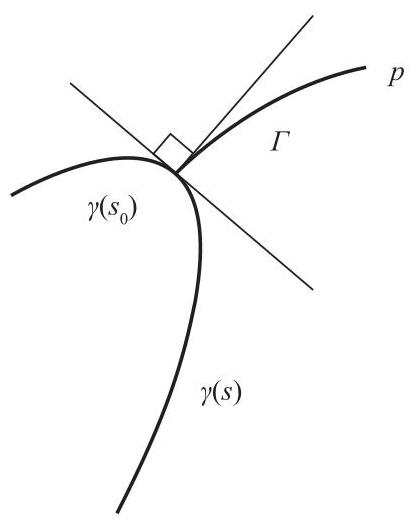
\includegraphics[max width=0.3\textwidth]{images/bo_d4b9jf3ef24c73e0334g_371_182_1026_417_529_0.jpg}
\end{center}
\hspace*{3em} 

图 5-14

c. 进一步假设 \(S\) 与平面同胚且具有高斯曲率 \(K \leq  0\) .证明 \({s}_{0}\) (因此 \(\Gamma\) )是唯一的.

4. (变分法.) 测地线是变分问题解的特例.在本练习中，我们将讨论一个简单但非常有代表性的变分问题的一些要点.在下一个练习中，我们将应用此处介绍的思想.

设 \(y = y\left( x\right) ,x \in  \left\lbrack  {{x}_{1},{x}_{2}}\right\rbrack\) 是 \({xy}\) 平面中的一条可微曲线，并设 \(y\) 的一个变分由可微映射 \(y = y\left( {x,t}\right)\) 给出， \(t \in  \left( {-\epsilon ,\epsilon }\right)\) .此处对所有 \(x \in  \left\lbrack  {{x}_{1},{x}_{2}}\right\rbrack\) 均有 \(y\left( {x,0}\right)  = y\left( x\right)\) ，对所有 \(t \in  \left( {-\epsilon ,\epsilon }\right)\) 均有 \(y\left( {{x}_{1},t}\right)  = \; y\left( {x}_{1}\right) ,y\left( {{x}_{2},t}\right)  = y\left( {x}_{2}\right)\) (即变分的端点固定).考虑积分

\[
I\left( t\right)  = {\int }_{{x}_{1}}^{{x}_{2}}F\left( {x,y\left( {x,t}\right) ,{y}^{\prime }\left( {x,t}\right) }\right) {dx},\;t \in  \left( {-\epsilon ,\epsilon }\right) ,
\]

其中 \(F\left( {x,y,{y}^{\prime }}\right)\) 是三个变量的可微函数， \({y}^{\prime } = \partial y/\partial x\) .寻找 \(I\left( t\right)\) 的临界点的问题称为以 \(F\) 为被积函数变分问题.

a. 假设曲线 \(y = y\left( x\right)\) 是 \(I\left( t\right)\) 的一个临界点(即对所有 \(t = 0\) 均有 \({dI}/{dt} = 0\) ).使用分部积分法得出 \(\left( {\dot{I} = {dI}/{dt}}\right)\)

\[
\dot{I}\left( t\right)  = {\int }_{{x}_{1}}^{{x}_{2}}\left( {{F}_{y}\frac{\partial y}{\partial t} + {F}_{{y}^{\prime }}\frac{\partial {y}^{\prime }}{\partial t}}\right) {dx}
\]

\[
= {\left\lbrack  \frac{\partial y}{\partial t}{F}_{{y}^{\prime }}\right\rbrack  }_{{x}_{1}}^{{x}_{2}} + {\int }_{{x}_{1}}^{{x}_{2}}\frac{\partial y}{\partial t}\left( {{F}_{y} - \frac{d}{dx}{F}_{{y}^{\prime }}}\right) {dx}.
\]

然后，利用边界条件，得到

\[
0 = \dot{I}\left( 0\right)  = {\int }_{{x}_{1}}^{{x}_{2}}\left\{  {\eta \left( {{F}_{y} - \frac{d}{dx}{F}_{{y}^{\prime }}}\right) }\right\}  {dx},
\]
 (*)

其中 \(\eta  = \left( {\partial y/\partial t}\right) \left( {x,0}\right)\) .(函数 \(\eta\) 对应于变分向量场或 \(y\left( {x,t}\right)\) .)

b. 证明如果对所有具有固定端点的变分(即对所有 \(\eta\) 在 \(\left( *\right)\) 中且 \(\left. {\eta \left( {x}_{1}\right)  = \eta \left( {x}_{2}\right)  = 0}\right)\) )均有 \(\dot{I}\left( 0\right)  = 0\) ，则

\[
{F}_{y} - \frac{d}{dx}{F}_{{y}^{\prime }} = 0.
\]
 (**)

方程(**)称为以 \(F\) 为被积函数的变分问题的欧拉-拉格朗日方程.

c. 证明如果 \(F\) 不显式地包含变量 \(x\) ，即 \(F = \; F\left( {y,{y}^{\prime }}\right)\) ，则通过对 \({y}^{\prime }{F}_{{y}^{\prime }} - F\) 求导，并使用(**)得到

\[
{y}^{\prime }{F}_{{y}^{\prime }} - F = \text{ const. }
\]

5.(变分法；应用.)

a.(最小面积的旋转曲面.)设 \(S\) 是通过将曲线 \(y = f\left( x\right) ,x \in  \left\lbrack  {{x}_{1},{x}_{2}}\right\rbrack\) 绕 \(x\) 轴旋转而得到的旋转曲面.假设 \(S\) 在连接 \(\left( {{x}_{1},f\left( {x}_{1}\right) }\right)\) 到 \(\left( {{x}_{2},f\left( {x}_{2}\right) }\right)\) 的所有旋转曲面中具有最小面积.因此， \(y = f\left( x\right)\) 最小化积分(参见练习 11，第 2-5 节)

\[
I\left( t\right)  = {\int }_{{x}_{1}}^{{x}_{2}}y\sqrt{1 + {\left( {y}^{\prime }\right) }^{2}}{dx}
\]

对所有具有固定端点 \(y\left( {x}_{1}\right) ,y\left( {x}_{2}\right)\) 的 \(y\) 的变分 \(y\left( {x,t}\right)\) .根据练习 4 的 b 部分， \(F\left( {y,{y}^{\prime }}\right)  = y\sqrt{1 + {\left( {y}^{\prime }\right) }^{2}}\) 满足欧拉-拉格朗日方程 \(\left( {* * }\right)\) .使用练习 4 的 \(c\) 部分得到

\[
{y}^{\prime }{F}_{{y}^{\prime }} - F =  - \frac{y}{\sqrt{1 + {\left( {y}^{\prime }\right) }^{2}}} =  - \frac{1}{c},\;c = \text{ const. };
\]

因此，

\[
y = \frac{1}{c}\cosh \left( {{cx} + {c}_{1}}\right) ,\;{c}_{1} = \text{ const. }
\]

若存在一个连接两个给定平行圆的最小面积的旋转曲面，则该曲面是链体面，且这两个给定圆是其平行线.

b. (旋转曲面的测地线.) 令

\[
\mathbf{x}\left( {u,v}\right)  = \left( {f\left( v\right) \cos u,f\left( v\right) \sin u,g\left( v\right) }\right)
\]

为旋转曲面 \(S\) 的参数化.令 \(u = u\left( v\right)\) 为 \(S\) 的一条既非平行线也非经线的测地线方程.则 \(u = u\left( v\right)\) 是弧长积分 \(\left( {F = 0}\right)\) 的一个临界点.

\[
\int \sqrt{E{\left( {u}^{\prime }\right) }^{2} + G}{dv},\;{u}^{\prime } = \frac{du}{dv}.
\]

由于 \(E = {f}^{2},G = {\left( {f}^{\prime }\right) }^{2} + {\left( {g}^{\prime }\right) }^{2}\) ，我们看到这个变分问题的欧拉-拉格朗日方程是

\[
{F}_{u} - \frac{d}{dv}{F}_{{u}^{\prime }} = 0,\;F = \sqrt{{f}^{2}{\left( {u}^{\prime }\right) }^{2} + {\left( {f}^{\prime }\right) }^{2} + {\left( {g}^{\prime }\right) }^{2}}.
\]

注意到 \(F\) 不依赖于 \(u\) .因此， \(\left( {d/{dv}}\right) {F}_{{u}^{\prime }} = 0\) ，并且

\[
c = \text{ const. } = {F}_{{u}^{\prime }} = \frac{{u}^{\prime }{f}^{2}}{\sqrt{{f}^{2}{\left( {u}^{\prime }\right) }^{2} + {\left( {f}^{\prime }\right) }^{2} + {\left( {g}^{\prime }\right) }^{2}}}.
\]

由此，得到测地线 \(u = u\left( v\right)\) 的以下方程(参见 4-4 节的例 5):

\[
u = c\int \frac{1}{f}\frac{\sqrt{{\left( {f}^{\prime }\right) }^{2} + {\left( {g}^{\prime }\right) }^{2}}}{{f}^{2} - {c}^{2}}{dv} + \text{ const. }
\]

\section*{5-5. 雅可比场与共轭点}

在本节中，我们将探讨用于证明邦内定理的变分技术的细节.

我们感兴趣的是获取关于给定测地线 \(\gamma\) 附近测地线行为的信息.自然的方法是考虑 \(\gamma\) 的变分，这些变分满足曲线本身也是测地线的附加条件.这种变分的变分场给出了测地线在 \(\gamma\) 邻域中分布密度的概念.

为简化表述，我们将假设曲面是完备的，尽管通过进一步的工作可以去掉这个假设.记号 \(\gamma  : \left\lbrack  {0,l}\right\rbrack   \rightarrow  S\) 将表示在完备曲面 \(S\) 上由弧长参数化的测地线.

定义 1. 令 \(\gamma  : \left\lbrack  {0,l}\right\rbrack   \rightarrow  S\) 为 \(S\) 上的参数化测地线，令 \(\mathrm{h} : \left\lbrack  {0,l}\right\rbrack   \times  \left( {-\epsilon ,\epsilon }\right)  \rightarrow  S\) 为 \(\gamma\) 的一个变分，使得对于每个 \(\mathrm{t} \in  \left( {-\epsilon ,\epsilon }\right)\) ，曲线 \({\mathrm{h}}_{\mathrm{t}}\left( S\right)  = \mathrm{h}\left( {S,\mathrm{t}}\right) ,S \in  \left\lbrack  {0,l}\right\rbrack\) 都是一个参数化测地线(不一定是按弧长参数化).变分场 \(\left( {\partial \mathrm{h}/\partial \mathrm{t}}\right) \left( {S,0}\right)  = \mathrm{J}\left( S\right)\) 称为沿 \(\gamma\) 的雅可比场.

雅可比场的一个平凡例子是由测地线 \(\gamma\) 的切向量场 \({\gamma }^{\prime }\left( s\right) ,s \in  \left\lbrack  {0,l}\right\rbrack\) 给出的.事实上，通过取 \(h\left( {s,t}\right)  = \gamma \left( {s + t}\right)\) ，我们得到

\[
J\left( s\right)  = \frac{\partial h}{\partial t}\left( {s,0}\right)  = \frac{d\gamma }{ds}.
\]

我们特别有兴趣研究从 \(\gamma \left( 0\right)\) 开始的、邻近 \(\gamma  : \left\lbrack  {0,l}\right\rbrack   \rightarrow  S\) 的测地线的行为.因此，我们将考虑满足条件 \(h\left( {0,t}\right)  = \gamma \left( 0\right)\) 、 \(t \in  \left( {-\epsilon ,\epsilon }\right)\) 的变分 \(h : \left\lbrack  {0,l}\right\rbrack   \times  \left( {-\epsilon ,\epsilon }\right)  \rightarrow  S\) .因此，相应的雅可比场满足条件 \(J\left( 0\right)  = 0\) (见图 5-15).

\begin{center}
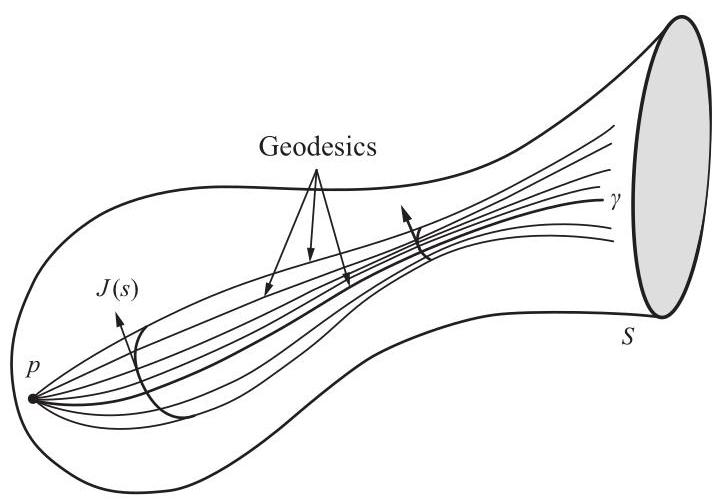
\includegraphics[max width=0.6\textwidth]{images/bo_d4b9jf3ef24c73e0334g_374_424_1541_720_500_0.jpg}
\end{center}
\hspace*{3em} 

图 5-15

在给出一个非平凡的雅可比场例子之前，我们将证明这样的场可以通过一个解析条件来表征.

命题 1. 设 \(\mathrm{J}\left( S\right)\) 是 \(\gamma  : \left\lbrack  {0,l}\right\rbrack   \rightarrow  S\) 、 \(S \in  \left\lbrack  {0,l}\right\rbrack\) 上的一个雅可比场.则 \(\mathrm{J}\) 满足所谓的雅可比方程

\[
\frac{\mathrm{D}}{\mathrm{{ds}}}\frac{\mathrm{D}}{\mathrm{{ds}}}\mathrm{J}\left( S\right)  + \mathrm{K}\left( S\right) \left( {{\gamma }^{\prime }\left( S\right)  \land  \mathrm{J}\left( S\right) }\right)  \land  {\gamma }^{\prime }\left( S\right)  = 0, \tag{1}
\]

其中 \(\mathrm{K}\left( S\right)\) 是 \(S\) 在 \(\gamma \left( S\right)\) 处的曲率.

证明.根据 \(J\left( s\right)\) 的定义，存在一个变分

\[
h : \left\lbrack  {0,l}\right\rbrack   \times  \left( {-\epsilon ,\epsilon }\right)  \rightarrow  S
\]

使得 \(\gamma\) 使得 \(\left( {\partial h/\partial t}\right) \left( {s,0}\right)  = J\left( s\right)\) 且 \({h}_{t}\left( s\right)\) 是测地线， \(t \in  \left( {-\epsilon ,\epsilon }\right)\) .由此可知 \(\left( {D/\partial s}\right) \left( {\partial h/\partial s}\right) \left( {s,t}\right)  = 0\) .因此，

\[
\frac{D}{\partial t}\frac{D}{\partial s}\frac{\partial h}{\partial s}\left( {s,t}\right)  = 0,\;\left( {s,t}\right)  \in  \left\lbrack  {0,l}\right\rbrack   \times  \left( {-\epsilon ,\epsilon }\right) .
\]

另一方面，利用第 5-4 节的引理 6，我们得到

\[
\frac{D}{\partial t}\frac{D}{\partial s}\frac{\partial h}{\partial s} = \frac{D}{\partial s}\frac{D}{\partial t}\frac{\partial h}{\partial s} + K\left( {s,t}\right) \left( {\frac{\partial h}{\partial s} \land  \frac{\partial h}{\partial t}}\right)  \land  \frac{\partial h}{\partial s} = 0.
\]

由于 \(\left( {D/\partial t}\right) \left( {\partial h/\partial s}\right)  = \left( {D/\partial s}\right) \left( {\partial h/\partial t}\right)\) ，我们对于 \(t = 0\) 有

\[
\frac{D}{\partial s}\frac{D}{\partial s}J\left( s\right)  + K\left( s\right) \left( {{\gamma }^{\prime }\left( s\right)  \land  J\left( s\right) }\right)  \land  {\gamma }^{\prime }\left( s\right)  = 0. \tag{Q.E.D.}
\]

为了从命题 1 中得出一些推论，将方程(1)的雅可比方程写成更熟悉的形式是方便的.为此，设 \({e}_{1}\left( 0\right)\) 和 \({e}_{2}\left( 0\right)\) 是切平面 \({T}_{\gamma \left( 0\right) }\left( S\right)\) 中的单位正交向量，并设 \({e}_{1}\left( s\right)\) 和 \({e}_{2}\left( s\right)\) 分别是 \({e}_{1}\left( 0\right)\) 和 \({e}_{2}\left( 0\right)\) 沿着 \(\gamma \left( s\right)\) 的平行移动.

假设

\[
J\left( s\right)  = {a}_{1}\left( s\right) {e}_{1}\left( s\right)  + {a}_{2}\left( s\right) {e}_{2}\left( s\right)
\]

对于某些函数 \({a}_{1} = {a}_{1}\left( s\right) ,{a}_{2} = {a}_{2}\left( s\right)\) .然后，利用上一节的引理 2 并为简化符号省略 \(s\) ，我们得到

\[
\frac{D}{\partial s}J = {a}_{1}^{\prime }{e}_{1} + {a}_{2}^{\prime }{e}_{2}
\]

\[
\frac{D}{\partial s}\frac{D}{\partial s}J = {a}_{1}^{\prime \prime }{e}_{1} + {a}_{2}^{\prime \prime }{e}_{2}
\]

另一方面，如果我们写成

\[
\left( {{\gamma }^{\prime } \land  J}\right)  \land  {\gamma }^{\prime } = {\lambda }_{1}{e}_{1} + {\lambda }_{2}{e}_{2},
\]

我们得到

\[
{\lambda }_{1}{e}_{1} + {\lambda }_{2}{e}_{2} = \left( {{\gamma }^{\prime } \land  \left( {{a}_{1}{e}_{1} + {a}_{2}{e}_{2}}\right) }\right)  \land  {\gamma }^{\prime }
\]

\[
= {a}_{1}\left( {{\gamma }^{\prime } \land  {e}_{1}}\right)  \land  {\gamma }^{\prime } + {a}_{2}\left( {{\gamma }^{\prime } \land  {e}_{2}}\right)  \land  {\gamma }^{\prime }.
\]

因此，通过令 \(\left\langle  {\left( {{\gamma }^{\prime } \land  {e}_{i}}\right)  \land  {\gamma }^{\prime },{e}_{j}}\right\rangle   = {\alpha }_{ij},i,j = 1,2\) ，我们得到

\[
{\lambda }_{1} = {a}_{1}{\alpha }_{11} + {a}_{2}{\alpha }_{21},\;{\lambda }_{2} = {a}_{1}{\alpha }_{12} + {a}_{2}{\alpha }_{22}.
\]

因此，方程 (1) 可写为

(1a)
\[
{a}_{1}^{\prime \prime } + K\left( {{\alpha }_{11}{a}_{1} + {\alpha }_{21}{a}_{2}}\right)  = 0,
\]

\[
{a}_{2}^{\prime \prime } + K\left( {{\alpha }_{12}{a}_{1} + {\alpha }_{22}{a}_{2}}\right)  = 0,
\]

其中所有元素都是 \(s\) 的函数.注意 (1a) 是一个二阶线性微分方程组.该方程组的解 \(\left( {{a}_{1}\left( s\right) ,{a}_{2}\left( s\right) }\right)  = J\left( s\right)\) 对每个 \(s \in  \left\lbrack  {0,l}\right\rbrack\) 都定义，并构成一个向量空间.此外，(1a)(或 (1))的解 \(J\left( s\right)\) 由初始条件 \(J\left( 0\right) ,\left( {{DJ}/\partial s}\right) \left( 0\right)\) 完全确定，解空间具有 \(2 \times  2 =\) 4 个维度.

可以证明，沿测地线 \(\gamma  : \left\lbrack  {0,l}\right\rbrack   \rightarrow  S\) 且满足方程 (1) 的每个向量场 \(J\left( s\right)\) 实际上是一个雅可比场.由于我们只对满足条件 \(J\left( 0\right)  = 0\) 的雅可比场 \(J\left( s\right)\) 感兴趣，因此我们仅在此特定情况下证明该命题.

我们将使用以下记法.设 \({T}_{p}\left( S\right) ,p \in  S\) 为 \(S\) 在点 \(p\) 处的切平面，并记 \({\left( {T}_{p}\left( S\right) \right) }_{v}\) 为在 \(v\) 处的切空间，将 \({T}_{p}\left( S\right)\) 视为 \({R}^{3}\) 中的一个曲面.由于 \({\exp }_{p} : {T}_{p}\left( S\right)  \rightarrow  S\) ，

\[
d{\left( {\exp }_{p}\right) }_{v} : {\left( {T}_{p}\left( S\right) \right) }_{v} \rightarrow  {T}_{{\exp }_{p}\left( v\right) }\left( S\right) .
\]

我们将经常进行以下记号滥用:如果 \(v,w \in  {T}_{p}\left( S\right)\) ，则 \(w\) 也表示 \({\left( {T}_{p}\left( S\right) \right) }_{v}\) 中的向量，该向量由将向量 \(v\) 平移 \(w\) 得到(参见图 5-16).这等价于通过向量 \(v\) 的平移来识别空间 \({T}_{p}\left( S\right)\) 和 \({\left( {T}_{p}\left( S\right) \right) }_{v}\) .

引理 1. 设 \(\mathrm{p} \in  S\) 且选择 \(\mathrm{v},\mathrm{w} \in  {\mathrm{T}}_{\mathrm{p}}\left( S\right)\) ，其中 \(\left| \mathrm{v}\right|  = 1\) .设 \(\gamma  : \left\lbrack  {0,l}\right\rbrack   \rightarrow  S\) 为 \(S\) 上的测地线，由下式给出

\[
\gamma \left( S\right)  = {\exp }_{\mathrm{p}}\left( \mathrm{{sv}}\right) ,\;S \in  \left\lbrack  {0,l}\right\rbrack  .
\]

那么，沿 \(\gamma\) 的向量场 \(\mathrm{J}\left( S\right)\) 由下式给出

\[
\mathrm{J}\left( S\right)  = S{\left( \mathrm{d}{\exp }_{\mathrm{p}}\right) }_{\mathrm{{sv}}}\left( \mathrm{w}\right) ,\;S \in  (0,l\rbrack ,
\]

是一个雅可比场.此外， \(\mathrm{J}\left( 0\right)  = 0,\left( {\mathrm{{DJ}}/\mathrm{{ds}}}\right) \left( 0\right)  = \mathrm{w}\) .

\begin{center}
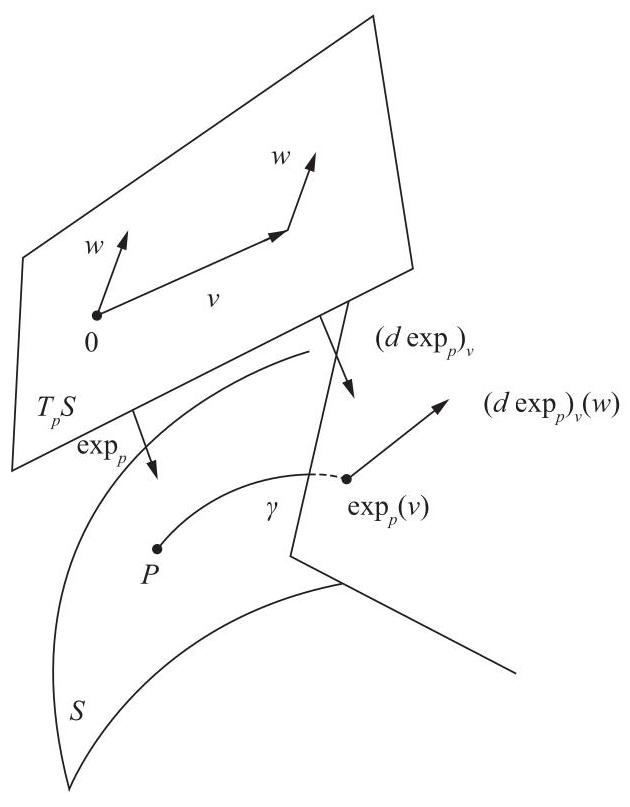
\includegraphics[max width=0.5\textwidth]{images/bo_d4b9jf3ef24c73e0334g_377_181_191_630_807_0.jpg}
\end{center}
\hspace*{3em} 

图 5-16

证明. 设 \(t \rightarrow  v\left( t\right) ,t \in  \left( {-\epsilon ,\epsilon }\right)\) 为 \({T}_{p}\left( S\right)\) 中的一个参数化曲线，使得 \(v\left( 0\right)  = v\) 和 \(\left( {{dv}/{dt}}\right) \left( 0\right)  = w\) .(请注意，我们正在进行上述记号滥用.)定义(参见图 5-17)

\[
h\left( {s,t}\right)  = {\exp }_{p}\left( {{sv}\left( t\right) }\right) ,\;t \in  \left( {-\epsilon ,\epsilon }\right) ,s \in  \left\lbrack  {0,l}\right\rbrack  .
\]

映射 \(h\) 显然是可微的，曲线 \(s \rightarrow  {h}_{t}\left( s\right)  = \; h\left( {s,t}\right)\) 是测地线 \(s \rightarrow  {\exp }_{p}\left( {{sv}\left( t\right) }\right)\) .因此， \(h\) 的变分场是 \(\gamma\) 上的雅可比场.

为了计算变分场 \(\left( {\partial h/\partial t}\right) \left( {s,0}\right)\) ，注意到 \({T}_{p}\left( S\right) ,s = {s}_{0},t = t\) 的曲线由 \(t \rightarrow  {s}_{0}v\left( t\right)\) 给出，并且该曲线在点 \(t = 0\) 处的切向量是

\[
{s}_{0}\frac{dv}{dt}\left( 0\right)  = {s}_{0}w
\]

由此可知

\[
\frac{\partial h}{\partial t}\left( {s,0}\right)  = {\left( d{\exp }_{p}\right) }_{sv}\left( {sw}\right)  = s{\left( d{\exp }_{p}\right) }_{sv}\left( w\right) .
\]

因此，向量场 \(J\left( s\right)  = s{\left( d{\exp }_{p}\right) }_{sv}\left( w\right)\) 是一个雅可比场.很容易验证 \(J\left( 0\right)  = 0\) .为了验证引理的最后论断，我们计算上述表达式的协变导数(参见引理 2，第 5-4 节)，得到

\[
\frac{D}{\partial s}s{\left( d{\exp }_{p}\right) }_{sv}\left( w\right)  = {\left( d{\exp }_{p}\right) }_{sv}\left( w\right)  + s\frac{D}{\partial s}{\left( d{\exp }_{p}\right) }_{sv}\left( w\right) .
\]

\begin{center}
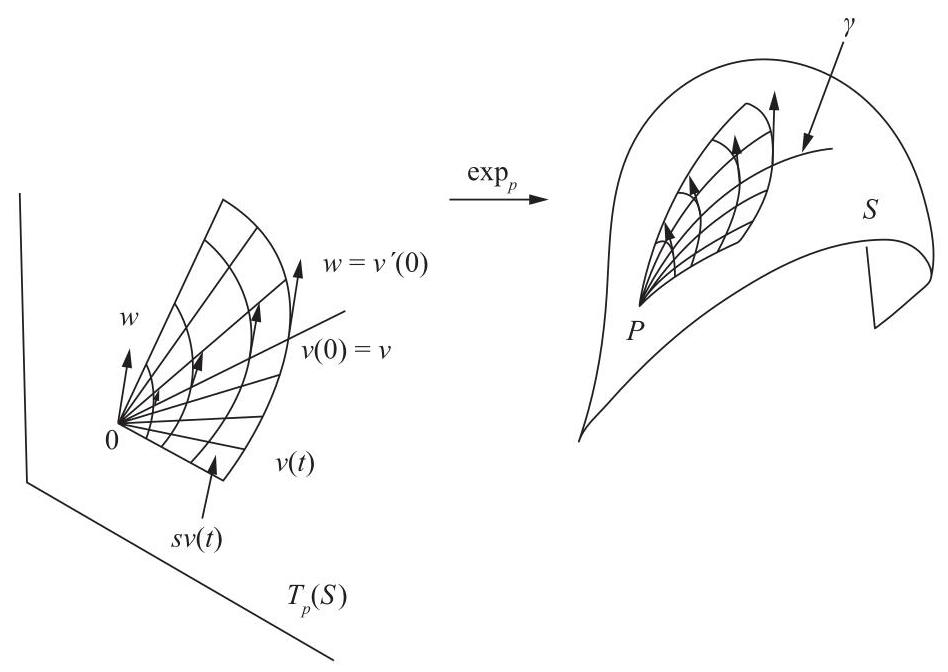
\includegraphics[max width=0.8\textwidth]{images/bo_d4b9jf3ef24c73e0334g_378_307_199_948_672_0.jpg}
\end{center}
\hspace*{3em} 

图 5-17

因此，在 \(s = 0\) 处，

\[
\frac{DJ}{\partial s}\left( 0\right)  = {\left( d{\exp }_{p}\right) }_{0}\left( w\right)  = w. \tag{Q.E.D.}
\]

命题 2. 如果令 \(\mathrm{J}\left( S\right)\) 为 \(\gamma  : \left\lbrack  {0,l}\right\rbrack   \rightarrow  S,S \in  \left\lbrack  {0,l}\right\rbrack\) 上的一个可微向量场，满足雅可比方程 (1)，且 \(\mathrm{J}\left( 0\right)  = 0\) ，则 \(\mathrm{J}\left( S\right)\) 是 \(\gamma\) 上的雅可比场.

证明. 令 \(w = \left( {{DJ}/{ds}}\right) \left( 0\right)\) 和 \(v = {\gamma }^{\prime }\left( 0\right)\) .根据引理 1，存在一个雅可比场 \(s{\left( d{\exp }_{p}\right) }_{sv}\left( w\right)  = \bar{J}\left( s\right) ,s \in  \left\lbrack  {0,l}\right\rbrack\) ，满足

\[
\bar{J}\left( 0\right)  = 0,\left( \frac{D\bar{J}}{ds}\right) \left( 0\right)  = w.
\]

那么， \(J\) 和 \(\bar{J}\) 是两个满足方程组 (1) 且具有相同初始条件的向量场.根据唯一性， \(J\left( s\right)  = \bar{J}\left( s\right) ,s \in  \left\lbrack  {0,l}\right\rbrack\) ；因此， \(J\) 是一个雅可比场.证毕.

现在我们可以给出一个非平凡的雅可比场例子了.

令 \({S}^{2} = \left\{  {\left( {x,y,z}\right)  \in  {R}^{3};{x}^{2} + {y}^{2} + {z}^{2} = 1}\right\}\) 为单位球面， \(\mathbf{x}\left( {\theta ,\varphi }\right)\) 为在 \(p \in  S\) 处的参数化，由余纬角 \(\theta\) 和经度 \(\varphi\) 给出(参见第 2-2 节，示例 1).考虑平行圈 \(\theta  = \pi /2\) 上介于 \({\varphi }_{0} = \pi /2\) 和 \({\varphi }_{1} = {3\pi }/2\) 之间的线段.该线段是一条测地线 \(\gamma\) ，我们假设它由 \(\varphi  - {\varphi }_{0} = s\) 参数化.令 \(w\left( s\right)\) 为沿 \(\gamma\) 的平行移动，移动一个向量 \(w\left( 0\right)  \in  {T}_{\gamma \left( 0\right) }\left( S\right)\) ，其中 \(\left| {w\left( 0\right) }\right|  = 1\) 和 \(\left\langle  {w\left( 0\right) ,{\gamma }^{\prime }\left( 0\right) }\right\rangle   = 0\) .我们将证明向量场(参见图 5-18)

\[
J\left( s\right)  = \left( {\sin s}\right) w\left( s\right) ,\;s \in  \left\lbrack  {0,\pi }\right\rbrack  ,
\]

\begin{center}
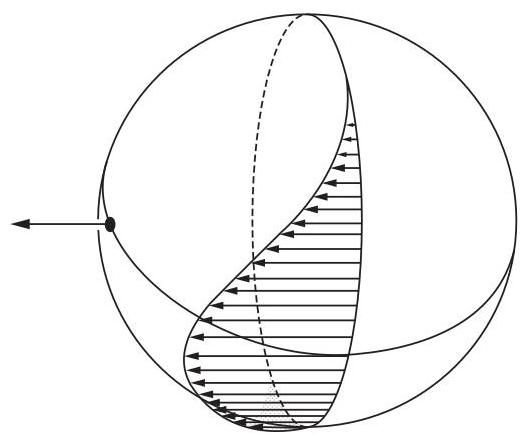
\includegraphics[max width=0.4\textwidth]{images/bo_d4b9jf3ef24c73e0334g_379_503_190_527_437_0.jpg}
\end{center}
\hspace*{3em} 

图 5-18. 球面上的雅可比场.

是 \(\gamma\) 上的一个雅可比场.

事实上，由于 \(J\left( 0\right)  = 0\) ，我们只需验证 \(J\) 满足方程 (1).利用 \(K = 1\) 和 \(w\) 是平行场这一事实，我们依次得到，

\[
\frac{DJ}{ds} = \left( {\cos s}\right) w\left( s\right)
\]

\[
\frac{D}{ds}\frac{DJ}{ds} = \left( {-\sin s}\right) w\left( s\right) ,
\]

\[
\frac{D}{ds}\frac{DJ}{ds} + K\left( {{\gamma }^{\prime } \land  J}\right)  \land  {\gamma }^{\prime } = \left( {-\sin s}\right) w\left( s\right)  + \left( {\sin s}\right) w\left( s\right)  = 0,
\]

这表明 \(J\) 是一个雅可比场.注意 \(J\left( \pi \right)  = 0\) .

定义 2. 令 \(\gamma  : \left\lbrack  {0,l}\right\rbrack   \rightarrow  S\) 为 \(S\) 的一条测地线，其中 \(\gamma \left( 0\right)  = \mathrm{p}\) .我们称点 \(\mathrm{q} = \gamma \left( {S}_{0}\right) ,{S}_{0} \in  \left\lbrack  {0,l}\right\rbrack\) 相对于测地线 \(\gamma\) 与 \(\mathrm{p}\) 共轭，如果存在一个非恒为零的雅可比场 \(\mathrm{J}\left( S\right)\) ，沿 \(\gamma\) 且 \(\mathrm{J}\left( 0\right)  = \mathrm{J}\left( {S}_{0}\right)  = 0\) .

正如我们在前面的例子中看到的，给定单位球面 \({S}^{2}\) 上的一个点 \(p \in  {S}^{2}\) ，其对径点与 \(p\) 共轭，沿任何从 \(p\) 开始的测地线.然而，球面的例子并不典型.一般来说，给定一个曲面 \(S\) 上的点 \(p\) ，与 \(p\) 的“第一个”共轭点 \(q\) 会随着我们改变通过 \(p\) 的测地线的方向而变化，并描述一个参数化曲线.该曲线的轨迹称为 \(p\) 的共轭轨迹，记为 \(C\left( p\right)\) .

\begin{center}
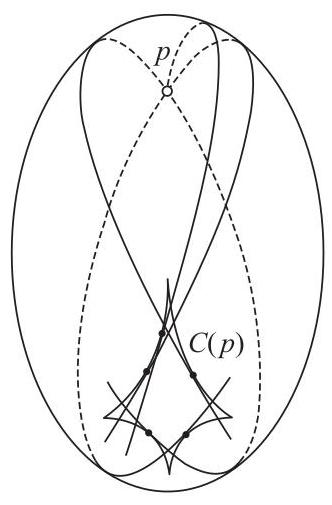
\includegraphics[max width=0.3\textwidth]{images/bo_d4b9jf3ef24c73e0334g_380_198_191_332_505_0.jpg}
\end{center}
\hspace*{3em} 

图 5-19. 椭球面的共轭轨迹.

图 5-19 展示了椭球的典型情况.从点 \(p\) 开始的测地线与曲线 \(C\left( p\right)\) 相切，使得当测地线 \(\overline{\gamma }\) 在 \(\gamma\) 附近接近 \(\gamma\) 时， \(\overline{\gamma }\) 和 \(\gamma\) 的交点接近 \(p\) 相对于 \(\gamma\) 的共轭点 \(q\) .这种情况用经典术语来说就是共轭点是两条“无限接近”的测地线的交点.

注 1. 在球面 \({S}^{2}\) 上，每一点 \(p \in  {S}^{2}\) 的共轭轨迹缩减为单点( \(p\) 的对径点)这一事实是一个特殊情况.事实上，可以证明球面是唯一具有此性质的曲面(参见 L. Green, "Aufwiedersehenfläche," Ann. Math. 78 (1963), 289-300).

注 2. 一般椭球的共轭轨迹由 A. Braunmühl, "Geodätische Linien auf dreiachsigen Flächen zweiten Grades," Math. Ann. 20 (1882), 557-586 确定.也可参见 H. Mangoldt, "Geodätische Linien auf positiv gekrümmten Flächen," Crelles Journ. 91 (1881), 23-52.

Jacobi 场 \(J\) 沿 \(\gamma  : \left\lbrack  {0,l}\right\rbrack   \rightarrow  S\) 的一个有用性质是，当 \(J\left( 0\right)  = J\left( l\right)  = 0\) 时，

\[
\left\langle  {J\left( s\right) ,{\gamma }^{\prime }\left( s\right) }\right\rangle   = 0
\]

对于每一个 \(s \in  \left\lbrack  {0,l}\right\rbrack\) .实际上，这是 Jacobi 场以下性质的结果.

命题 3. 设 \({\mathrm{J}}_{1}\left( \mathrm{\;s}\right)\) 和 \({\mathrm{J}}_{2}\left( \mathrm{\;s}\right)\) 是沿 \(\gamma  : \left\lbrack  {0,l}\right\rbrack   \rightarrow \; S,S \in  \left\lbrack  {0,l}\right\rbrack\) 的 Jacobi 场.则

\[
\left\langle  {\frac{D{J}_{1}}{ds},{J}_{2}\left( s\right) }\right\rangle   - \left\langle  {{J}_{1}\left( s\right) ,\frac{D{J}_{2}}{ds}}\right\rangle   = \text{ const. }
\]

证明. 只需对陈述的表达式求导并应用命题 1(为方便表示，省略了 \(s\) ):

\[
\frac{d}{ds}\left\{  {\left\langle  {\frac{D{J}_{1}}{ds},{J}_{2}}\right\rangle   - \left\langle  {{J}_{1},\frac{D{J}_{2}}{ds}}\right\rangle  }\right\}
\]

\[
= \left\langle  {\frac{D}{ds}\frac{D{J}_{1}}{ds},{J}_{2}}\right\rangle   - \left\langle  {{J}_{1},\frac{D}{ds}\frac{D{J}_{2}}{ds}}\right\rangle   + \left\langle  {\frac{D{J}_{1}}{ds},\frac{D{J}_{2}}{ds}}\right\rangle   - \left\langle  {\frac{D{J}_{1}}{ds},\frac{D{J}_{2}}{ds}}\right\rangle
\]

\[
=  - K\left\{  {\left\langle  {{\gamma }^{\prime } \land  {J}_{1}}\right\rangle   \land  {\gamma }^{\prime },{J}_{2}}\right\}   - \left\langle  {\left( {{\gamma }^{\prime } \land  {J}_{2}}\right)  \land  {\gamma }^{\prime },{J}_{1}}\right\rangle  \}  = 0. \tag{Q.E.D.}
\]

命题 4. 设 \(\mathrm{J}\left( S\right)\) 是沿 \(\gamma  : \left\lbrack  {0,l}\right\rbrack   \rightarrow  S\) 的 Jacobi 场，且

\[
\left\langle  {J\left( {s}_{1}\right) ,{\gamma }^{\prime }\left( {s}_{1}\right) }\right\rangle   = \left\langle  {J\left( {s}_{2}\right) ,{\gamma }^{\prime }\left( {s}_{2}\right) }\right\rangle   = 0,\;{s}_{1},{s}_{2} \in  \left\lbrack  {0,l}\right\rbrack  ,{s}_{1} \neq  {s}_{2}.
\]

则

\[
\left\langle  {J\left( s\right) ,{\gamma }^{\prime }\left( s\right) }\right\rangle   = 0,\;s \in  \left\lbrack  {0,l}\right\rbrack  .
\]

证明. 我们将 \({J}_{1}\left( s\right)  = J\left( s\right)\) 和 \({J}_{2}\left( s\right)  = {\gamma }^{\prime }\left( s\right)\) (这是一个 Jacobi 场)代入前一个命题，得到

\[
\left\langle  {\frac{DJ}{ds},{\gamma }^{\prime }\left( s\right) }\right\rangle   = \text{ const. } = A.
\]

因此，

\[
\frac{d}{ds}\left\langle  {J\left( s\right) ,{\gamma }^{\prime }\left( s\right) }\right\rangle   = \left\langle  {\frac{DJ}{ds},{\gamma }^{\prime }\left( s\right) }\right\rangle   = A;
\]

所以，

\[
\left\langle  {J\left( s\right) ,{\gamma }^{\prime }\left( s\right) }\right\rangle   = {As} + B,
\]

其中 \(B\) 是常数.由于线性表达式 \({As} + B\) 对于 \({s}_{1}\) 和 \({s}_{2} \in  \left\lbrack  {0,l}\right\rbrack  ,{s}_{1} \neq  {s}_{2}\) 为零，因此它恒为零.Q.E.D.

推论. 设 \(\mathrm{J}\left( S\right)\) 是沿 \(\gamma  : \left\lbrack  {0,l}\right\rbrack   \rightarrow  S\) 的 Jacobi 场，且 \(\mathrm{J}\left( 0\right)  = \mathrm{J}\left( l\right)  = 0\) .则 \(\langle \mathrm{J}\left( S\right) ,{\gamma }^{\prime }\left( S\right) \rangle  = 0,\mathrm{\;s} \in  \left\lbrack  {0,l}\right\rbrack\) .

现在我们将证明共轭点可以通过指数映射的行为来刻画.回想一下，当 \(\varphi  : {S}_{1} \rightarrow  {S}_{2}\) 是正则曲面 \({S}_{1}\) 到正则曲面 \({S}_{2}\) 的一个可微映射时，如果线性映射 \(\varphi\) 是奇异的，则称点 \(p \in  {S}_{1}\) 是 \(\varphi\) 的一个临界点.

\[
d{\varphi }_{p} : {T}_{p}\left( {S}_{1}\right)  \rightarrow  {T}_{\varphi \left( p\right) }\left( {S}_{2}\right)
\]

是奇异的，也就是说，如果存在 \(v \in  {T}_{p}\left( {S}_{1}\right) ,v \neq  0\) ，其中 \(d{\varphi }_{p}\left( v\right)  = 0\) .

命题 5. 设 \(\mathrm{p},\mathrm{q} \in  S\) 是 \(S\) 的两个点，设 \(\gamma  : \left\lbrack  {0,l}\right\rbrack   \rightarrow  S\) 是连接 \(\mathrm{p} = \gamma \left( 0\right)\) 到 \(\mathrm{q} = {\exp }_{\mathrm{p}}\left( {l{\gamma }^{\prime }\left( 0\right) }\right)\) 的测地线.则 \(\mathrm{q}\) 相对于 \(\gamma\) 与 \(\mathrm{p}\) 共轭，当且仅当 \(\mathrm{v} = l{\gamma }^{\prime }\left( 0\right)\) 是 \(\operatorname{ex}{p}_{\mathrm{p}}\) : \({\mathrm{T}}_{\mathrm{p}}\left( S\right)  \rightarrow  S\) 的一个临界点.

证明. 正如我们在引理 1 中看到的，对于每一个 \(w \in  {T}_{p}\left( S\right)\) (我们将其与 \({\left( {T}_{p}\left( S\right) \right) }_{v}\) 视为相同)，都存在一个沿 \(\gamma\) 的 Jacobi 场 \(J\left( s\right)\) ，使得

\[
J\left( 0\right)  = 0,
\]

\[
\frac{DJ}{ds}\left( 0\right)  = w
\]

和

\[
J\left( l\right)  = l\left\{  {{\left( d{\exp }_{p}\right) }_{v}\left( w\right) }\right\}
\]

如果 \(v \in  {T}_{p}\left( S\right)\) 是 \({\exp }_{p}\) 的一个临界点，则存在 \(w \in  {T}_{p}\left( S\right) {)}_{v},w \neq  0\) ，其中 \({\left( d{\exp }_{p}\right) }_{v}\left( w\right)  = 0\) .这意味着上述向量场 \(J\left( s\right)\) 不恒为零，并且 \(J\left( 0\right)  = J\left( l\right)  = 0\) ；也就是说，相对于 \(\gamma\) ， \(\gamma \left( l\right)\) 与 \(\gamma \left( 0\right)\) 共轭.

反之，如果相对于 \(\gamma\) ， \(q = \gamma \left( l\right)\) 与 \(p = \gamma \left( 0\right)\) 共轭，则存在一个非恒为零的 Jacobi 场 \(\bar{J}\left( s\right)\) ，使得 \(\bar{J}\left( 0\right)  = \bar{J}\left( l\right)  = 0\) .设 \(\left( {D\bar{J}/{ds}}\right) \left( 0\right)  = w \neq  0\) .通过如上构造一个 Jacobi 场 \(J\left( s\right)\) ，我们根据唯一性得到 \(\bar{J}\left( s\right)  = J\left( s\right)\) .因为

\[
J\left( l\right)  = l\left\{  {{\left( d{\exp }_{p}\right) }_{v}\left( w\right) }\right\}   = \bar{J}\left( l\right)  = 0,
\]

我们得出 \({\left( d{\exp }_{p}\right) }_{v}\left( w\right)  = 0\) ，其中 \(w \neq  0\) .因此 \(v\) 是 \({\exp }_{p}\) 的一个临界点.证毕.

Jacobi 场方程 (1) 涉及 \(S\) 的高斯曲率 \(K\) ，这表明从某点 \(p \in  S\) 出发的测地线“散开”的现象与 \(S\) 中曲率的分布密切相关(参见第 4-6 节的注记 2).从某点 \(p \in  S\) 出发的两条相邻测地线最初会相互远离，这是一个基本事实.在球体或椭球体 \(\left( {K > \delta  > 0}\right)\) 的情况下，它们会重新靠近并与共轭轨迹 \(C\left( p\right)\) 相切.在平面情况下，它们永远不会再次靠近.下面的定理表明，平面情况的“无穷小版本”出现在曲率为负或零的曲面上.(参见定理证明后的注记 3.)

定理 1. 假设曲面 \(S\) 的高斯曲率 \(\mathrm{K}\) 满足条件 \(\mathrm{K} \leq  0\) .那么，对于任意 \(\mathrm{p} \in  S\) ， \(\mathrm{p}\) 的共轭轨迹为空.简而言之，曲率为 \(\mathrm{K} \leq  0\) 的曲面没有共轭点.

证明. 令 \(p \in  S\) ，并令 \(\gamma  : \left\lbrack  {0,l}\right\rbrack   \rightarrow  S\) 为 \(S\) 上的一条测地线，且 \(\gamma \left( 0\right)  = p\) .假设存在一个非零的 Jacobi 场 \(J\left( s\right)\) ，且 \(J\left( 0\right)  = J\left( l\right)  = 0\) .我们将证明这会产生矛盾.

事实上，由于 \(J\left( s\right)\) 是一个 Jacobi 场且 \(J\left( 0\right)  = J\left( l\right)  = 0\) ，根据命题 4 的推论，我们有 \(\left\langle  {J\left( s\right) ,{\gamma }^{\prime }\left( s\right) }\right\rangle   = 0,s \in  \left\lbrack  {0,l}\right\rbrack\) .因此，

\[
\frac{D}{ds}\frac{DJ}{ds} + {KJ} = 0
\]

\[
\left\langle  {\frac{D}{ds}\frac{DJ}{ds},J}\right\rangle   =  - K\langle J,J\rangle  \geq  0
\]

由于 \(K \leq  0\) .

由此得出

\[
\frac{d}{ds}\left\langle  {\frac{DJ}{ds},J}\right\rangle   = \left\langle  {\frac{D}{ds}\frac{DJ}{ds},J}\right\rangle   + \left\langle  {\frac{DJ}{ds},\frac{DJ}{ds}}\right\rangle   \geq  0.
\]

因此，函数 \(\langle {DJ}/{ds},J\rangle\) 在区间 \(\left\lbrack  {0,l}\right\rbrack\) 上不减.由于该函数在 \(s = 0\) 时为零且在 \(s = l\) 时为零，我们得出结论:

\[
\left\langle  {\frac{DJ}{ds},J\left( s\right) }\right\rangle   = 0,\;s \in  \left\lbrack  {0,l}\right\rbrack  .
\]

最后，通过观察

\[
\frac{d}{ds}\langle J,J\rangle  = 2\left\langle  {\frac{DJ}{ds},J}\right\rangle   = 0,
\]

我们得到 \({\left| J\right| }^{2} =\) 为常数.由于 \(J\left( 0\right)  = 0\) ，我们得出 \(\left| {J\left( s\right) }\right|  = 0,s \in  \left\lbrack  {0,l}\right\rbrack\) ；也就是说， \(J\) 在 \(\left\lbrack  {0,l}\right\rbrack\) 中恒等于零.这产生了矛盾.Q.E.D.

注记 3. 该定理并未断言从给定点出发的两条测地线永远不会再次相遇.实际上，这是错误的，如圆柱体的闭合测地线所示，其曲率为零.即使我们考虑从给定点出发且具有“附近方向”的测地线，该断言也不成立.考虑圆柱体的子午线并观察到遵循接近子午线方向的螺旋线会与该子午线相遇就足够了.该命题所断言的是，两条“相邻”测地线的交点随着这些测地线相互靠近而趋于“无穷大”(这正是圆柱体中发生的情况).用经典的术语来说，我们可以说两条“无穷接近”的测地线永远不会相遇.从这个意义上说，该定理是平面情况的无穷小版本.

命题 5、上述定理和反函数定理的直接推论是以下推论.

推论. 假设 \(\mathrm{K}\) 的 \(S\) 的高斯曲率为负或零. 那么对于每一个 \(\mathrm{p} \in  S\) ,映射

\[
{\exp }_{\mathrm{p}} : {\mathrm{T}}_{\mathrm{p}}\left( S\right)  \rightarrow  S
\]

是一个局部微分同胚.

我们稍后将使用以下引理, 它推广了在 \(p\) 的法邻域中, 测地圆与径向测地线正交的事实 (见 4-6 节, 命题 3 和注 1).

引理 2 (高斯). 令 \(\mathrm{p} \in  S\) 为 (完备) 曲面 \(S\) 上的一点, 令 \(\mathrm{u} \in  {\mathrm{T}}_{\mathrm{p}}\left( S\right)\) 和 \(\mathrm{w} \in  {\left( {\mathrm{T}}_{\mathrm{p}}\left( \mathrm{\;S}\right) \right) }_{\mathrm{u}}\) . 则

\[
\langle \mathrm{u},\mathrm{w}\rangle  = \left\langle  {{\left( \mathrm{d}{\exp }_{\mathrm{p}}\right) }_{\mathrm{u}}\left( \mathrm{u}\right) ,{\left( \mathrm{d}{\exp }_{\mathrm{p}}\right) }_{\mathrm{u}}\left( \mathrm{w}\right) }\right\rangle  ,
\]

其中使用了 \({\mathrm{T}}_{\mathrm{p}}\left( S\right)  \approx  {\left( {\mathrm{T}}_{\mathrm{p}}\left( S\right) \right) }_{\mathrm{u}}\) 的等同.

证明. 令 \(l = \left| u\right| ,v = u/\left| u\right|\) ,令 \(\gamma  : \left\lbrack  {0,l}\right\rbrack   \rightarrow  S\) 为 \(S\) 上的一条测地线, 由

\[
\gamma \left( s\right)  = {\exp }_{p}\left( {sv}\right) ,\;s \in  \left\lbrack  {0,l}\right\rbrack  .
\]

则 \({\gamma }^{\prime }\left( 0\right)  = v\) . 此外,如果我们考虑 \({T}_{p}\left( S\right)\) 中通过 \(u\) 的曲线 \(s \rightarrow  {sv}\) 对于 \(s = l\) ,其切向量为 \(v\) (见图 5-20), 我们得到

\[
{\gamma }^{\prime }\left( l\right)  = {\left. \frac{d}{ds}\left( {\exp }_{p}sv\right) \right| }_{s = l} = {\left( d{\exp }_{p}\right) }_{u}\left( v\right) .
\]

\begin{center}
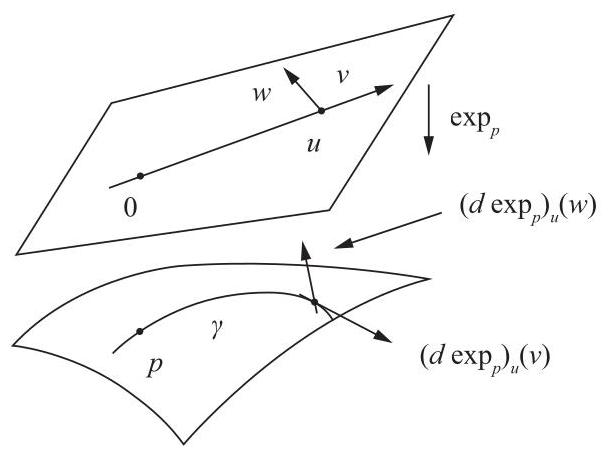
\includegraphics[max width=0.5\textwidth]{images/bo_d4b9jf3ef24c73e0334g_384_198_1153_608_458_0.jpg}
\end{center}
\hspace*{3em} 

图 5-20

现在考虑 \(\gamma\) 上的一条雅可比场 \(J\) ,由 \(J\left( 0\right)  = 0,\left( {{DJ}/{ds}}\right) \left( 0\right)  = w\) 给出 (参见引理 1). 那么,由于 \(\gamma \left( s\right)\) 是一条测地线,

\[
\frac{d}{ds}\left\langle  {{\gamma }^{\prime }\left( s\right) ,J\left( s\right) }\right\rangle   = \left\langle  {{\gamma }^{\prime }\left( s\right) ,\frac{DJ}{ds}}\right\rangle  ,
\]

并且由于 \(J\) 是一个雅可比场,

\[
\frac{d}{ds}\left\langle  {{\gamma }^{\prime }\left( s\right) ,\frac{DJ}{ds}}\right\rangle   = \left\langle  {{\gamma }^{\prime }\left( s\right) ,\frac{{D}^{2}J}{d{s}^{2}}}\right\rangle   = 0.
\]

由此得出

\[
\frac{d}{ds}\left\langle  {{\gamma }^{\prime }\left( s\right) ,J\left( s\right) }\right\rangle   = \left\langle  {{\gamma }^{\prime }\left( s\right) ,\frac{DJ}{ds}}\right\rangle   = \text{ const. } = C; \tag{2}
\]

因此 (由于 \(J\left( 0\right)  = 0\) )

\[
\left\langle  {{\gamma }^{\prime }\left( s\right) ,J\left( s\right) }\right\rangle   = {Cs}. \tag{3}
\]

为了计算常数 \(C\) ,将式 (3) 中的 \(l\) 设置为等于. 根据引理 1,

\[
J\left( l\right)  = l{\left( d{\exp }_{p}\right) }_{u}\left( w\right) .
\]

因此,

\[
{Cl} = \left\langle  {{\gamma }^{\prime }\left( l\right) ,J\left( l\right) }\right\rangle   = \left\langle  {{\left( d{\exp }_{p}\right) }_{u}\left( v\right) ,l{\left( d{\exp }_{p}\right) }_{u}\left( w\right) }\right\rangle  .
\]

从式 (2) 我们得出

\[
\left\langle  {{\gamma }^{\prime }\left( l\right) ,\frac{DJ}{ds}\left( l\right) }\right\rangle   = C = \left\langle  {{\gamma }^{\prime }\left( 0\right) ,\frac{DJ}{ds}\left( 0\right) }\right\rangle   = \langle v,w\rangle .
\]

利用 \(C\) 的值,我们从上述表达式得到

\[
\langle u,w\rangle  = \left\langle  {{\left( d{\exp }_{p}\right) }_{u}\left( u\right) ,{\left( d{\exp }_{p}\right) }_{u}\left( w\right) }\right\rangle  . \tag{Q.E.D.}
\]

\exerciseline

1. a. 设 \(\gamma  : \left\lbrack  {0,l}\right\rbrack   \rightarrow  S\) 是曲面 \(S\) 上一条由弧长参数化的测地线，设 \(J\left( s\right)\) 是 \(\gamma\) 上的一条雅可比场，满足 \(J\left( 0\right)  = 0\) ， \(\left\langle  {{J}^{\prime }\left( 0\right) ,{\gamma }^{\prime }\left( 0\right) }\right\rangle   = 0\) .证明对于所有 \(s \in  \left\lbrack  {0,l}\right\rbrack\) ，都有 \(\left\langle  {J\left( s\right) ,{\gamma }^{\prime }\left( s\right) }\right\rangle   = 0\) .

b. 进一步假设 \(\left| {{J}^{\prime }\left( 0\right) }\right|  = 1\) .对 \({e}_{1}\left( 0\right)  = \; {\gamma }^{\prime }\left( 0\right)\) 和 \({e}_{2}\left( 0\right)  = {J}^{\prime }\left( 0\right)\) 沿 \(\gamma\) 进行平行移动，得到正交基 \(\left\{  {{e}_{1}\left( s\right) ,{e}_{2}\left( s\right) }\right\}\) ，对于所有 \({T}_{\gamma \left( s\right) }\left( S\right) ,s \in  \left\lbrack  {0,l}\right\rbrack\) .根据 a 部分，对于某个函数 \(u = u\left( s\right)\) ，有 \(J\left( s\right)  = u\left( s\right) {e}_{2}\left( s\right)\) .证明 \(J\) 的雅可比方程可以写成

\[
{u}^{\prime \prime }\left( s\right)  + K\left( s\right) u\left( s\right)  = 0,
\]

初始条件为 \(u\left( 0\right)  = 0,{u}^{\prime }\left( 0\right)  = 1\) .

2. 证明抛物面 \(z = {x}^{2} + {y}^{2}\) 上的点 \(p = \left( {0,0,0}\right)\) 相对于测地线 \(\gamma \left( s\right)\) (满足 \(\gamma \left( 0\right)  = p\) )没有共轭点.

3. (比较定理.)设 \(S\) 和 \(\widetilde{S}\) 为完备曲面.设 \(p \in  S\) , \(\widetilde{p} \in  \widetilde{S}\) 并选择一个线性等距 \(i : {T}_{p}\left( S\right)  \rightarrow  {T}_{\widetilde{p}}\left( \widetilde{S}\right)\) .设 \(\gamma  : \lbrack 0,\infty ) \rightarrow  S\) 是 \(S\) 上的一条测地线，其 \(\gamma \left( 0\right)  = p,\left| {{\gamma }^{\prime }\left( 0\right) }\right|  = 1\) ，设 \(J\left( s\right)\) 是 \(\gamma\) 上的一条雅可比场，其 \(J\left( 0\right)  = 0,\left\langle  {{J}^{\prime }\left( 0\right) ,{\gamma }^{\prime }\left( 0\right) }\right\rangle   = 0,\left| {{J}^{\prime }\left( 0\right) }\right|  = 1\) .利用线性等距 \(i\) ，构造一条测地线 \(\widetilde{\gamma } : \lbrack 0,\infty ) \rightarrow  \widetilde{S}\) ，其 \(\widetilde{\gamma }\left( 0\right)  = \widetilde{p}\) , \({\widetilde{\gamma }}^{\prime }\left( 0\right)  = i\left( {{\gamma }^{\prime }\left( 0\right) }\right)\) ，以及一条雅可比场 \(\widetilde{J}\) ，其在 \(\widetilde{\gamma }\) 上，具有 \(\widetilde{J}\left( 0\right)  = 0,{\widetilde{J}}^{\prime }\left( 0\right)  = \; i\left( {{J}^{\prime }\left( 0\right) }\right)\) (图 5-21).下面我们将描述两个定理(它们本质上是经典 Sturm 比较定理的几何解释)，它们允许我们从 \(S\) 和 \(\widetilde{S}\) 的曲率的“比较假设”来比较雅可比场 \(J\) 和 \(\widetilde{J}\) .

\begin{center}
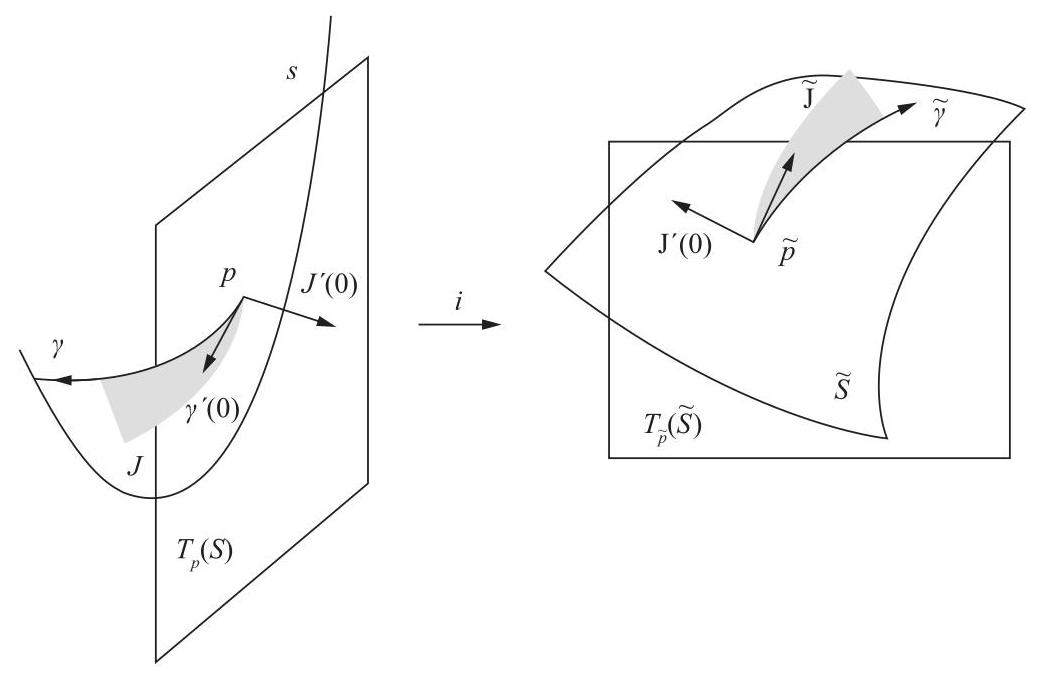
\includegraphics[max width=0.9\textwidth]{images/bo_d4b9jf3ef24c73e0334g_386_262_189_1041_674_0.jpg}
\end{center}
\hspace*{3em} 

图 5-21

a. 使用练习 1 表明，对于可微函数 \(u = u\left( s\right) ,v = v\left( s\right)\) ， \(J\left( s\right)  = v\left( s\right) {e}_{2}\left( s\right) ,\widetilde{J}\left( s\right)  = u\left( s\right) {\widetilde{e}}_{2}\left( s\right)\) ，其中 \({e}_{2}\left( s\right)\) (分别表示 \({\widetilde{e}}_{2}\left( s\right)\) ) 是 \({J}^{\prime }\left( 0\right)\) (分别表示 \({\widetilde{J}}^{\prime }\left( 0\right)\) ) 沿 \(\gamma\) (分别表示 \(\widetilde{\gamma }\) ) 的平行移动.得出 \(J\) 和 \(\widetilde{J}\) 的雅可比方程为

\[
{v}^{\prime \prime }\left( s\right)  + K\left( s\right) v\left( s\right)  = 0,\;v\left( 0\right)  = 0,{v}^{\prime }\left( 0\right)  = 1,
\]

\[
{u}^{\prime \prime }\left( s\right)  + K\left( s\right) u\left( s\right)  = 0,\;u\left( 0\right)  = 0,{u}^{\prime }\left( 0\right)  = 1,
\]

分别表示，其中 \(K\) 和 \(\widetilde{K}\) 表示 \(S\) 和 \(\widetilde{S}\) 的高斯曲率.

*b. 假设 \(K\left( s\right)  \leq  \widetilde{K}\left( s\right) ,s \in  \left\lbrack  {0,\infty }\right\rbrack\) .证明

(*)
\[
0 = {\int }_{0}^{s}\left\{  {u\left( {{v}^{\prime \prime } + {Kv}}\right)  - v\left( {{u}^{\prime \prime } + \widetilde{K}u}\right) }\right\}  {ds}
\]

\[
= {\left\lbrack  u{v}^{\prime } - v{u}^{\prime }\right\rbrack  }_{0}^{s} + {\int }_{0}^{s}\left( {K - \widetilde{K}}\right) {uvds}.
\]

得出结论，如果 \(a\) 是 \(u\) 在 \(\left( {0,\infty }\right)\) 中的第一个零点(即 \(u\left( a\right)  = 0\) 且 \(u\left( s\right)  > 0\) 在 \(\left( {0,a}\right) )\) 中)，而 \(b\) 是 \(v\) 在 \(\left( {0,\infty }\right)\) 中的第一个零点，则 \(b \geq  a\) .因此，如果对于所有 \(S\) 都有 \(\mathrm{K}\left( S\right)  \leq  \widetilde{\mathrm{K}}\left( S\right)\) ，则 \(\mathrm{p}\) 相对于 \(\gamma\) 的第一个共轭点不会出现在 \(\widetilde{\mathrm{p}}\) 相对于 \(\widetilde{\gamma }\) 的第一个共轭点之前.这被称为第一个比较定理.

*c. 假设 \(K\left( s\right)  \leq  \widetilde{K}\left( s\right) ,s \in  \lbrack 0,a)\) .使用 (*) 和 \(u\) 和 \(v\) 在 \(\left( {0,a}\right)\) 中为正这一事实，得到 \({\left\lbrack  u{v}^{\prime } - v{u}^{\prime }\right\rbrack  }_{0}^{s} \geq  0\) .使用此不等式证明对于所有 \(s \in  \left( {0,a}\right)\) 都有 \(v\left( s\right)  \geq  u\left( s\right)\) .因此，如果对于第一个共轭点 \(\widetilde{\gamma }\) 之前的所有 s 都有 \(\mathrm{K}\left( S\right)  \leq  \widetilde{\mathrm{K}}\left( S\right)\) ，则对于所有这样的 s 都有 \(\left| {\mathrm{J}\left( S\right) }\right|  \geq  \left| {\widetilde{\mathrm{J}}\left( S\right) }\right|\) .这被称为第二个比较定理(当然，这包括第一个作为特例；我们之所以单独列出第一个情况，是因为它更简单，而且是我们更常用的).

d. 证明在部分 \(c\) 中，当且仅当 \(K\left( s\right)  = \widetilde{K}\left( s\right) ,s \in  \lbrack 0,a)\) 时，对于所有 \(s \in  \lbrack 0,a)\) 等式 \(v\left( s\right)  = u\left( s\right)\) 成立.

4. 令 \(S\) 为一个具有高斯曲率 \(K \leq  {K}_{0}\) 的完备曲面，其中 \({K}_{0}\) 是一个正常数.将 \(S\) 与曲率为 \({K}_{0}\) 的球面 \({S}^{2}\left( {K}_{0}\right)\) 进行比较(即，在练习 3 中，令 \(\widetilde{S} = {S}^{2}\left( {K}_{0}\right)\) 并使用第一个比较定理，练习 3，部分 b)得出结论， \(S\) 上的任何测地线 \(\gamma  : \lbrack 0,\infty ) \rightarrow  S\) 在区间 \(\left( {0,\pi /\sqrt{{K}_{0}}}\right)\) 中没有与 \(\gamma \left( 0\right)\) 共轭的点.

5. 令 \(S\) 为一个完备曲面，其 \(K \geq  {K}_{1} > 0\) ，其中 \(K\) 是 \(S\) 的高斯曲率，而 \({K}_{1}\) 是一个常数.证明每条测地线 \(\gamma  : \lbrack 0,\infty ) \rightarrow  S\) 在区间 \(\left( {0,\pi /\sqrt{{K}_{1}}}\right\rbrack\) 中都有一个与 \(\gamma \left( 0\right)\) 共轭的点.

*6. (Sturm振荡定理.) 下面是第一个比较定理(习题3，b部分)的一个稍加推广的版本，它经常很有用.设 \(S\) 是一个完备曲面， \(\gamma  : \lbrack 0,\infty ) \rightarrow  S\) 是 \(S\) 上的一个测地线.设 \(J\left( s\right)\) 是 \(\gamma\) 上一个Jacobi场，满足 \(J\left( 0\right)  = J\left( {s}_{0}\right)  = 0,{s}_{0} \in  \left( {0,\infty }\right)\) 和 \(J\left( s\right)  \neq  0\) ，对于 \(s \in  \left( {0,{s}_{0}}\right)\) .因此， \(J\left( s\right)\) 是一个法向场(命题4的推论).由此可知 \(J\left( s\right)  = v\left( s\right) {e}_{2}\left( s\right)\) ，其中 \(v\left( s\right)\) 是以下方程的解:

\[
{v}^{\prime \prime }\left( s\right)  + K\left( s\right) v\left( s\right)  = 0,\;s \in  \lbrack 0,\infty ),
\]

并且 \({e}_{2}\left( s\right)\) 是 \({T}_{\gamma \left( 0\right) }\left( S\right)\) 上一个垂直于 \({\gamma }^{\prime }\left( 0\right)\) 的单位向量在 \({\gamma }^{\prime }\left( 0\right)\) 上的平行移动.假设 \(S\) 的高斯曲率 \(K\left( s\right)\) 满足 \(K\left( s\right)  \leq  L\left( s\right)\) ，其中 \(L\) 是 \(\lbrack 0,\infty )\) 上的一个可微函数.证明任何满足

\[
{u}^{\prime \prime }\left( s\right)  + L\left( s\right) u\left( s\right)  = 0,\;s \in  \lbrack 0,\infty ),
\]

的解在区间 \(\left( {0,{s}_{0}}\right\rbrack\) 内有一个零点(即存在 \({s}_{1} \in  \left( {0,{s}_{0}}\right\rbrack\) 使得 \(\left. {u\left( {s}_{1}\right)  = 0}\right)\) ).

7. (Kneser共轭点判据.) 设 \(S\) 是一个完备曲面， \(\gamma  : \lbrack 0,\infty ) \rightarrow  S\) 是 \(S\) 上的一条测地线，满足 \(\gamma \left( 0\right)  = p\) .设 \(K\left( s\right)\) 是 \(S\) 沿 \(\gamma\) 的高斯曲率.假设

\[
{\int }_{t}^{\infty }K\left( s\right) {ds} \leq  \frac{1}{4\left( {t + 1}\right) }\text{ for all }t \geq  0
\]
 (*)

表示积分收敛且如指示般有界.

a. 定义

\[
w\left( t\right)  = {\int }_{t}^{\infty }K\left( s\right) {ds} + \frac{1}{4\left( {t + 1}\right) },\;t \geq  0,
\]

并证明 \({w}^{\prime }\left( t\right)  + {\left( w\left( t\right) \right) }^{2} \leq   - K\left( t\right)\) .

b. 令 \(t \geq  0,{w}^{\prime }\left( t\right)  + {\left( w\left( t\right) \right) }^{2} =  - L\left( t\right)\) (使得 \(L\left( t\right)  \geq  K\left( t\right)\) )，并定义

\[
v\left( t\right)  = \exp \left( {{\int }_{0}^{t}w\left( s\right) {ds}}\right) ,\;t \geq  0.
\]

证明 \({v}^{\prime \prime }\left( t\right)  + L\left( t\right) v\left( t\right)  = 0,v\left( 0\right)  = 1,{v}^{\prime }\left( 0\right)  = 0\) .

c. 注意到 \(v\left( t\right)  > 0\) ，并使用 Sturm 振动定理(练习 6)证明不存在沿 \(\gamma \left( s\right)\) 且满足 \(J\left( 0\right)  = 0\) 和 \(J\left( {s}_{0}\right)  = 0,{s}_{0} \in  \left( {0,\infty }\right)\) 的 Jacobi 场 \(J\left( s\right)\) .因此，如果 \(\left( *\right)\) 成立，则不存在沿 \(\gamma\) 与 \(\mathrm{p}\) 共轭的点.

*8. 令 \(\gamma  : \left\lbrack  {0,l}\right\rbrack   \rightarrow  S\) 为完备曲面 \(S\) 上的一条测地线，并假设 \(\gamma \left( l\right)\) 不与 \(\gamma \left( 0\right)\) 共轭.令 \({w}_{0} \in  {T}_{\gamma \left( 0\right) }\left( S\right)\) 和 \({w}_{1} \in  {T}_{\gamma \left( l\right) }\left( S\right)\) .证明存在一条沿 \(\gamma\) 且满足 \(J\left( 0\right)  = {w}_{0}\) 、 \(J\left( l\right)  = {w}_{1}.\) 的唯一 Jacobi 场 \(J\left( s\right)\) .

9. 令 \(J\left( s\right)\) 为测地线 \(\gamma  : \left\lbrack  {0,l}\right\rbrack   \rightarrow  S\) 上的一条 Jacobi 场，使得 \(\left\langle  {J\left( 0\right) ,{\gamma }^{\prime }\left( 0\right) }\right\rangle   = 0\) 和 \({J}^{\prime }\left( 0\right)  = 0\) .证明对于所有 \(s \in  \left\lbrack  {0,l}\right\rbrack\) ，都有 \(\left\langle  {J\left( s\right) ,{\gamma }^{\prime }\left( s\right) }\right\rangle   = 0\) .

\section*{5-6. 覆盖空间；Hadamard 定理}

我们在上一节中看到，当完备曲面 \(S\) 的曲率 \(K\) 满足条件 \(K \leq  0\) 时，映射 \({\exp }_{p} : {T}_{p}\left( S\right)  \rightarrow  S,p \in  S\) 是一个局部微分同胚.自然会问，这个局部微分同胚何时是全局微分同胚.为了引入我们需要的覆盖空间概念，将这个问题置于更一般的环境中是方便的.

\section*{A. 覆盖空间}

定义 1. 令 \(\widetilde{\mathrm{B}}\) 和 \(\mathrm{B}\) 为 \({\mathbb{R}}^{3}\) 的子集.如果满足以下条件，我们称 \(\pi  : \widetilde{\mathrm{B}} \rightarrow  \mathrm{B}\) 为覆盖映射:

1. \(\pi\) 是连续的且 \(\pi \left( \widetilde{\mathrm{B}}\right)  = \mathrm{B}\) .

2. 每个点 \(\mathrm{p} \in  \mathrm{B}\) 都有一个邻域 \(\mathrm{U}\) 在 \(\mathrm{B}\) 中(称为 \(\mathrm{p}\) 的一个特殊邻域)，使得

\[
{\pi }^{-1}\left( \mathrm{U}\right)  = \mathop{\bigcup }\limits_{\alpha }{\mathrm{V}}_{\alpha }
\]

其中 \({\mathrm{V}}_{\alpha }\) 是成对不相交的开集，使得 \(\pi\) 在 \({\mathrm{V}}_{\alpha }\) 上的限制是 \({\mathrm{V}}_{\alpha }\) 到 \(\mathrm{U}\) 的一个同胚.

\(\widetilde{\mathrm{B}}\) 称为 \(\mathrm{B}\) 的覆盖空间.

示例 1. 令 \(P \subset  {R}^{3}\) 为 \({R}^{3}\) 的平面.通过固定一个点 \({q}_{0} \in  P\) 和两个正交单位向量 \({e}_{1},{e}_{2} \in  P\) ，原点在 \({q}_{0}\) ，每个点 \(q \in  P\) 都由坐标 \(\left( {u,v}\right)  = q\) 表征，其中

\[
q - {u}_{0} = u{e}_{1} + v{e}_{2}.
\]

现在令 \(S = \left\{  {\left( {x,y,z}\right)  \in  {R}^{3};{x}^{2} + {y}^{2} = 1}\right\}\) 为右圆柱体，其轴为 \(z\) 轴，令 \(\pi  : P \rightarrow  S\) 为由以下方式定义的映射

\[
\pi \left( {u,v}\right)  = \left( {\cos u,\sin u,v}\right)
\]

(该映射的几何意义是将平面 \(P\) 无限次地缠绕到圆柱体 \(S\) 上；见图 5-22).

\begin{center}
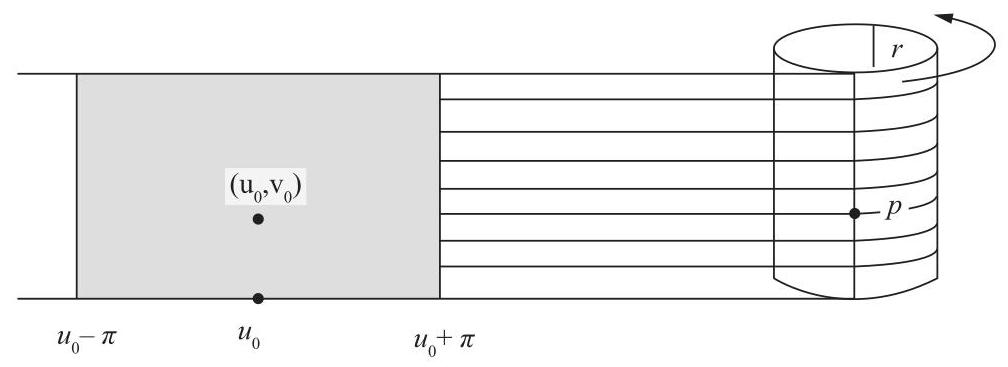
\includegraphics[max width=0.9\textwidth]{images/bo_d4b9jf3ef24c73e0334g_389_261_1222_1008_367_0.jpg}
\end{center}
\hspace*{3em} 

图 5-22

我们将证明 \(\pi\) 是一个覆盖映射.我们首先观察到，当 \(\left( {{u}_{0},{v}_{0}}\right)  \in  P\) 时，映射 \(\pi\) 在带状区域上的限制

\[
R = \left\{  {\left( {u,v}\right)  \in  P;{u}_{0} - \pi  \leq  u \leq  {u}_{0} + \pi }\right\}
\]

完全覆盖 \(S\) .实际上， \(\pi\) 在 \(R\) 内部上的限制是 \(S\) 的参数化，其坐标邻域覆盖了 \(S\) 减去一个生成元.因此， \(\pi\) 是连续的(实际上是可微的)，并且 \(\pi \left( P\right)  = S\) ，从而验证了条件 1.

为了验证条件 2，令 \(p \in  S\) 和 \(U = S - r\) ，其中 \(r\) 是与通过 \(p\) 的生成元相对的生成元.我们将证明 \(U\) 是 \(p\) 的一个特殊邻域.

令 \(\left( {{u}_{0},{v}_{0}}\right)  \in  P\) 使得 \(\pi \left( {{u}_{0},{v}_{0}}\right)  = p\) ，并选择 \({V}_{n}\) 为由以下方式给出的带状区域

\[
{V}_{n} = \left\{  {\left( {u,v}\right)  \in  P;{u}_{0} + \left( {{2n} - 1}\right) \pi  < u < {u}_{0} + \left( {{2n} + 1}\right) \pi }\right\}  ,
\]

\[
n = 0, \pm  1, \pm  2,\ldots
\]

可以立即验证，如果 \(n \neq  m\) ，则 \({V}_{n} \cap  {V}_{m} = \phi\) 且 \(\mathop{\bigcup }\limits_{n}{V}_{n} = \; {\pi }^{-1}\left( U\right)\) .此外，根据初始观察， \(\pi\) 在任何 \({V}_{n}\) 上的限制都是到 \(U\) 的一个同胚.因此， \(U\) 是 \(p\) 的一个特殊邻域.这验证了条件 2，并表明平面 \(P\) 是圆柱体 \(S\) 的一个覆盖空间.

示例 2. 令 \(H\) 为螺旋线

\[
H = \left\{  {\left( {x,y,z}\right)  \subset  {R}^{3};x = \cos t,y = \sin t;z = {bt},t \in  R}\right\}
\]

并令

\[
{S}^{1} = \left\{  {\left( {x,y,0}\right)  \in  {R}^{3};{x}^{2} + {y}^{2} = 1}\right\}
\]

为单位圆.令 \(\pi  : H \rightarrow  {S}^{1}\) 由以下方式定义

\[
\pi \left( {x,y,z}\right)  = \left( {x,y,0}\right) .
\]

我们将证明 \(\pi\) 是一个覆盖映射(参见图 5-23).

\begin{center}
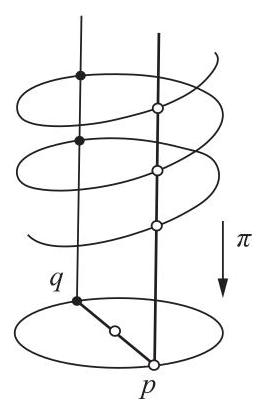
\includegraphics[max width=0.2\textwidth]{images/bo_d4b9jf3ef24c73e0334g_390_195_1473_264_411_0.jpg}
\end{center}
\hspace*{3em} 

图 5-23

显然 \(\pi\) 是连续的，并且 \(\pi \left( H\right)  = {S}^{1}\) .这验证了条件 1.

为了验证条件 2，令 \(p \in  {S}^{1}\) .我们将证明 \(U = {S}^{1} - \{ q\}\) ，其中 \(q \in  {S}^{1}\) 是与 \(p\) 对称的点，是 \(p\) 的一个区分邻域.事实上，令 \({t}_{0} \in  R\) 使得

\[
\pi \left( {\cos {t}_{0},\sin {t}_{0},b{t}_{0}}\right)  = p.
\]

我们取螺旋线对应于区间 \({V}_{n}\) 的弧段.

\[
\left( {{t}_{0} + \left( {{2n} - 1}\right) \pi ,{t}_{0} + \left( {{2n} + 1}\right) \pi }\right)  \subset  R,\;n = 0, \pm  1, \pm  2,\ldots .
\]

那么很容易证明 \({\pi }^{-1}\left( U\right)  = \mathop{\bigcup }\limits_{n}{V}_{n}\) ， \({V}_{n}\) 是两两不相交的，并且 \(\pi\) 在 \({V}_{n}\) 上的限制是到 \(U\) 的一个同胚.这验证了条件 2 并结束了该例子.

现在，令 \(\pi  : \widetilde{B} \rightarrow  B\) 是一个覆盖映射.由于 \(\pi \left( \widetilde{B}\right)  = B\) ，每个点 \(\widetilde{p} \in  \widetilde{B}\) 使得 \(\widetilde{p} \in  {\pi }^{-1}\left( p\right)\) 对于某个 \(p \in  B\) .因此，存在 \(\widetilde{p}\) 的一个邻域 \({V}_{\alpha }\) 使得 \(\pi\) 在 \({V}_{\alpha }\) 上的限制是一个同胚.由此可知 \(\pi\) 是一个局部同胚.然而，下面的例子表明，存在不是覆盖映射的局部同胚.

在给出例子之前，应该注意到，如果 \(U\) 是 \(p\) 的一个区分邻域，那么 \(p\) 的每个邻域 \(\bar{U}\) 使得 \(\bar{U} \subset  U\) 又是 \(p\) 的一个区分邻域.由于 \({\pi }^{-1}\left( \bar{U}\right)  \subset  \mathop{\bigcup }\limits_{\alpha }{V}_{\alpha }\) 和 \({V}_{\alpha }\) 是两两不相交的，我们得到

\[
{\pi }^{-1}\left( \bar{U}\right)  = \mathop{\bigcup }\limits_{\alpha }{W}_{\alpha }
\]

其中集合 \({W}_{\alpha } = {\pi }^{-1}\left( \bar{U}\right)  \cap  {V}_{\alpha }\) 仍然满足定义 1 的条件 2 的不相交性.这样，在处理区分邻域时，我们可以将自己限制在“小”邻域上.

例子 3. 在例子 2 中考虑螺旋线 \(H\) 对应于区间 \(\left( {\pi ,{4\pi }}\right)  \subset  R\) 的一段 \(\widetilde{H}\) .显然， \(\pi\) 在该螺旋线开段上的限制 \(\widetilde{\pi }\) 仍然是一个局部同胚，并且 \(\widetilde{\pi }\left( \widetilde{H}\right)  = {S}^{1}\) .然而，没有一个邻域

\[
\pi \left( {\cos {3\pi },\sin {3\pi },{b3\pi }}\right)  = \left( {-1,0,0}\right)  = p \in  {S}^{1}
\]

可以是一个杰出的邻域.事实上，通过取 \(U\) 足够小， \({\widetilde{\pi }}^{-1}\left( U\right)  = {V}_{1} \cup  {V}_{2}\) ，其中 \({V}_{1}\) 是对应于 \(t \in \; \left( {\pi ,\pi  + \epsilon }\right)\) 的螺旋段，而 \({V}_{2}\) 是对应于 \(t \in  \left( {{3\pi } - \epsilon ,{3\pi } + \epsilon }\right)\) 的段.现在 \(\widetilde{\pi }\) 限制在 \({V}_{1}\) 上不是到 \(U\) 的同胚，因为 \(\widetilde{\pi }\left( {V}_{1}\right)\) 甚至不包含 \(p\) .因此， \(\widetilde{\pi } : \widetilde{H} \rightarrow  S\) 是到 \({S}^{1}\) 的局部同胚，但不是覆盖映射.

我们现在可以用以下更一般形式重述本节开头提出的问题:在什么条件下，局部同胚是全局同胚？

覆盖空间的概念允许我们将这个问题分解为以下两个问题:

1. 在什么条件下，局部同胚是覆盖映射？

2. 在什么条件下，覆盖映射是全局同胚？

以下命题给出了问题 1 的一个简单答案.

命题 1. 令 \(\pi  : \widetilde{\mathrm{B}} \rightarrow  \mathrm{B}\) 为局部同胚， \(\widetilde{\mathrm{B}}\) 为紧致集， \(\mathrm{B}\) 为连通集.则 \(\pi\) 是覆盖映射.

证明.由于 \(\pi\) 是局部同胚， \(\pi \left( \widetilde{B}\right)  \subset  B\) 在 \(B\) 中是开集.此外，由于 \(\pi ,\pi \left( \widetilde{B}\right)\) 的连续性， \(\pi \left( \widetilde{B}\right)  \subset  B\) 是紧致的，因此在 \(B\) 中是闭集.由于 \(\pi \left( \widetilde{B}\right)  \subset  B\) 在连通集 \(B,\pi \left( \widetilde{B}\right)  = B\) 中既是开集又是闭集.因此，定义 1 的条件 1 得到验证.

为了验证条件 2，令 \(b \in  B\) .则 \({\pi }^{-1}\left( b\right)  \subset  \widetilde{B}\) 是有限的.否则，它将有一个极限点 \(\widetilde{q} \in  \widetilde{B}\) ，这将与 \(\pi  : \widetilde{B} \rightarrow  B\) 是局部同胚的事实相矛盾.因此，我们可以写 \({\pi }^{-1}\left( b\right)  = \left\{  {{\widetilde{b}}_{1},\ldots ,{\widetilde{b}}_{k}}\right\}\) .

令 \({W}_{i}\) 为 \({\widetilde{b}}_{i},i = 1,\ldots ,k\) 的一个邻域，使得 \(\pi\) 在 \({W}_{i}\) 上的限制是一个同胚( \(\pi\) 是一个局部同胚).由于 \({\pi }^{-1}\left( b\right)\) 是有限的，可以选择足够小的 \({W}_{i}\) 使得它们两两不相交.由于 \(\widetilde{B}\) 是紧致的且 \(\pi\) 是连续的， \(\widetilde{B}\) 中闭集的像在 \(B\) 中也是闭集.因此存在 \(b\) 的一个邻域 \(U\) ，使得 \(U \subset  \mathop{\bigcap }\limits_{i}\pi \left( {W}_{i}\right)\) 和 \({\pi }^{-1}\left( U\right)  \subset  { \cup  }_{i}{W}_{i}\) (见图 5-24 和本章附录 E 节的命题).通过令 \({V}_{i} = {\pi }^{-1}U \cap  {W}_{i}\) ，我们得到

\[
{\pi }^{-1}\left( U\right)  = \mathop{\bigcup }\limits_{i}{V}_{i}
\]

并且 \({V}_{i}\) 两两不相交.此外， \(\pi\) 在 \({V}_{i}\) 上的限制显然是到 \(U\) 的一个同胚.因此 \(U\) 是 \(p\) 的一个特殊邻域.这验证了条件 2 并完成了证明.证毕.

\begin{center}
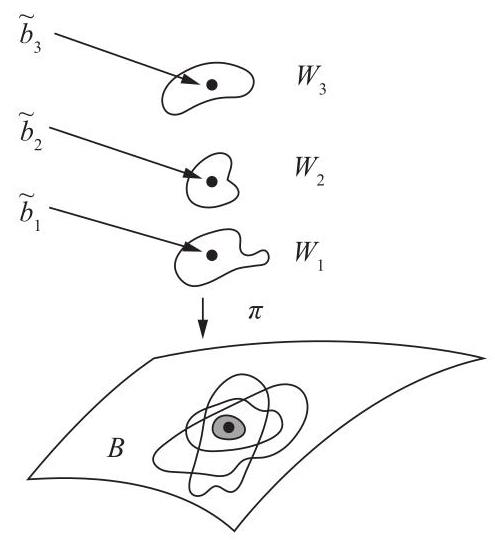
\includegraphics[max width=0.4\textwidth]{images/bo_d4b9jf3ef24c73e0334g_392_531_1501_495_540_0.jpg}
\end{center}
\hspace*{3em} 

图 5-24

当 \(\widetilde{B}\) 不紧致时，断言局部同胚是覆盖映射的有用判据很少.一个特例将在后面处理.对于这个特例以及对问题 2 的处理，我们需要回到覆盖空间.

覆盖映射最重要的性质是将 \(B\) 中的连续曲线“提升”到 \(\widetilde{B}\) 的可能性.更确切地说，我们将引入以下术语.

令 \(B \subset  {R}^{3}\) .回想一下，连续映射 \(\alpha  : \left\lbrack  {0,l}\right\rbrack   \rightarrow  B,\left\lbrack  {0,l}\right\rbrack   \subset  R\) 被称为 \(B\) 的一条弧(见第 5 章附录，定义 8).现在，令 \(\widetilde{B}\) 和 \(B\) 为 \({R}^{3}\) 的子集.令 \(\pi  : \widetilde{B} \rightarrow  B\) 为一个连续映射，令 \(\alpha  : \left\lbrack  {0,l}\right\rbrack   \rightarrow  B\) 为 \(B\) 的一条弧.如果存在 \(\widetilde{B}\) 的一条弧，

\[
\widetilde{\alpha } : \left\lbrack  {0,l}\right\rbrack   \rightarrow  \widetilde{B}
\]

与 \(\pi  \circ  \widetilde{\alpha } = \alpha ,\widetilde{\alpha }\) ，则称其为以 \(\widetilde{\alpha }\left( 0\right)  \in  \widetilde{B}\) 为起点的 \(\alpha\) 的提升.这种情况在附带的图示中进行了描述.

\begin{center}
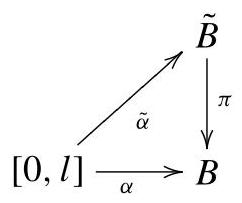
\includegraphics[max width=0.2\textwidth]{images/bo_d4b9jf3ef24c73e0334g_393_598_950_242_203_0.jpg}
\end{center}
\hspace*{3em} 

使用上述术语，覆盖空间的一个基本性质由以下存在性和唯一性命题表达.

命题 2. 设 \(\pi  : \widetilde{\mathrm{B}} \rightarrow  \mathrm{B}\) 是一个覆盖映射， \(\alpha  : \left\lbrack  {0,l}\right\rbrack   \rightarrow  \mathrm{B}\) 是 \(\mathrm{B}\) 中的一条弧，以及 \({\widetilde{\mathrm{p}}}_{0} \in  \widetilde{\mathrm{B}}\) 是 \(\widetilde{\mathrm{B}}\) 中的一点，使得 \(\pi \left( {\widetilde{\mathrm{p}}}_{0}\right)  = \alpha \left( 0\right)  = {\mathrm{p}}_{0}\) .则存在 \(\alpha\) 的一个唯一提升 \(\widetilde{\alpha } : \left\lbrack  {0,l}\right\rbrack   \rightarrow  \widetilde{\mathrm{B}}\) ，其起点为 \({\widetilde{\mathrm{p}}}_{0}\) ，即 \(\widetilde{\alpha }\left( 0\right)  = {\widetilde{\mathrm{p}}}_{0}.\) .

证明.我们首先证明唯一性.设 \(\widetilde{\alpha },\widetilde{\beta } : \left\lbrack  {0,l}\right\rbrack   \rightarrow  \widetilde{B}\) 是 \(\alpha\) 在 \({\widetilde{p}}_{0}\) 起点的两个提升.设 \(A \subset  \left\lbrack  {0,l}\right\rbrack\) 是点集 \(t \in  \left\lbrack  {0,l}\right\rbrack\) ，使得 \(\widetilde{\alpha }\left( t\right)  = \widetilde{\beta }\left( t\right) .A\) 非空，并且显然在 \(\left\lbrack  {0,l}\right\rbrack\) 中是闭集.

我们将证明 \(A\) 在 \(\left\lbrack  {0,l}\right\rbrack\) 中是开集.假设 \(\widetilde{\alpha }\left( t\right)  = \widetilde{\beta }\left( t\right)  = \widetilde{p}\) .考虑 \(\widetilde{p}\) 在 \(\left\lbrack  {0,l}\right\rbrack\) 中的一个邻域 \(V\) ，其中 \(\pi\) 是一个同胚.由于 \(\widetilde{\alpha }\) 和 \(\widetilde{\beta }\) 是连续映射，存在一个包含 \(t\) 的开区间 \({I}_{t} \subset  \left\lbrack  {0,l}\right\rbrack\) ，使得 \(\widetilde{\alpha }\left( {I}_{t}\right)  \subset  V\) 和 \(\widetilde{\beta }\left( {I}_{t}\right)  \subset  V\) .由于 \(\pi  \circ  \widetilde{\alpha } = \pi  \circ  \widetilde{\beta }\) 和 \(\pi\) 是 \(V,\widetilde{\alpha } = \widetilde{\beta }\) 在 \({I}_{t}\) 中的同胚，因此 \(A\) 是开集.由此得出 \(A = \left\lbrack  {0,l}\right\rbrack\) ，并且对于每一个 \(t \in  (0,l\rbrack\) ，这两个提升都重合.

现在我们证明存在性.由于 \(\alpha\) 是连续的，对于每一个 \(\alpha \left( t\right)  \in  B\) ，存在一个包含 \(t\) 的区间 \({I}_{t} \subset  \left\lbrack  {0,l}\right\rbrack\) ，使得 \(\alpha \left( {I}_{t}\right)\) 包含在一个特殊的邻域 \(\alpha \left( t\right)\) 中.族 \({I}_{t},t \in  \left\lbrack  {0,l}\right\rbrack\) 是 \(\left\lbrack  {0,l}\right\rbrack\) 的一个开覆盖，由于 \(\left\lbrack  {0,l}\right\rbrack\) 的紧致性，它允许一个有限子覆盖，例如 \({I}_{0},\ldots ,{I}_{n}\) .

\begin{center}
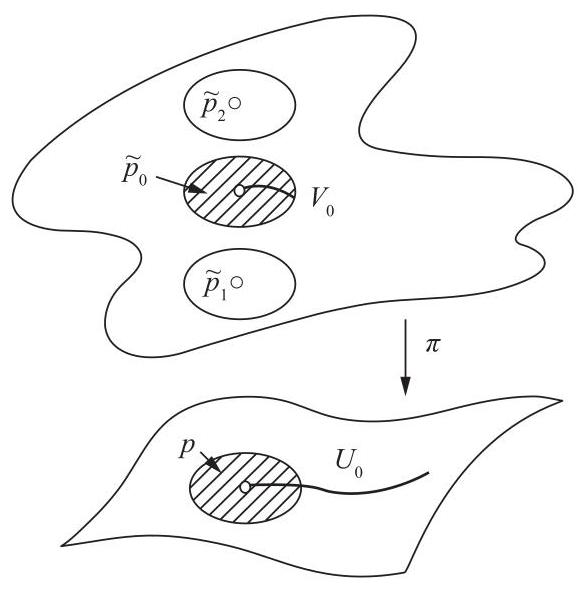
\includegraphics[max width=0.5\textwidth]{images/bo_d4b9jf3ef24c73e0334g_394_199_189_582_590_0.jpg}
\end{center}
\hspace*{3em} 

图 5-25

假设 \(0 \in  {I}_{0}\) .(否则，我们将更改区间的枚举.)由于 \(\alpha \left( {I}_{0}\right)\) 包含在 \(p\) 的一个特殊邻域 \({U}_{0}\) 中，因此存在 \({\widetilde{p}}_{0}\) 的一个邻域 \({V}_{0}\) ，使得 \(\pi\) 在 \({V}_{0}\) 上的限制 \({\pi }_{0}\) 是到 \({U}_{0}\) 的一个同胚.我们定义，对于 \(t \in  {I}_{0}\) (见图 5-25)，

\[
\widetilde{\alpha }\left( t\right)  = {\pi }_{0}^{-1} \circ  \alpha \left( t\right) ,
\]

其中 \({\pi }_{0}^{-1}\) 是同胚 \({\pi }_{0}\) 在 \({U}_{0}\) 中的逆映射.显然

\[
\widetilde{\alpha }\left( 0\right)  = {\widetilde{p}}_{0},
\]

\[
\pi  \circ  \widetilde{\alpha }\left( t\right)  = \alpha \left( t\right) ,\;t \in  {I}_{0}.
\]

现在假设 \({I}_{1} \cap  {I}_{0} \neq  \phi\) (否则我们将更改区间的顺序).令 \({t}_{1} \in  {I}_{1} \cap  {I}_{0}\) .由于 \(\alpha \left( {I}_{1}\right)\) 包含在 \(\alpha \left( {t}_{1}\right)\) 的一个特殊邻域 \({U}_{1}\) 中，我们可以定义一个以 \(\widetilde{\alpha }\left( {t}_{1}\right)\) 为起点的 \({I}_{1}\) 中 \(\alpha\) 的提升.根据唯一性，这条弧在 \({I}_{1} \cap  {I}_{0}\) 中与 \(\widetilde{\alpha }\) 一致，因此它是 \(\widetilde{\alpha }\) 到 \({I}_{0} \cup  {I}_{1}\) 的一个扩展.通过这种方式，我们构建了一条弧 \(\widetilde{\alpha }\left\lbrack  {0,l}\right\rbrack   \rightarrow  \widetilde{B}\) ，使得 \(\widetilde{\alpha }\left( 0\right)  = {\widetilde{p}}_{0}\) 和 \(\pi  \circ  \widetilde{\alpha }\left( t\right)  = \alpha \left( t\right) ,t \in  \left\lbrack  {0,l}\right\rbrack\) . \(\;\mathbf{Q}\) .证毕.

覆盖映射 \(\pi  : \widetilde{B} \rightarrow  B\) 的弧提升性质的一个有趣推论是，当 \(B\) 是弧连通的时，集合 \({\pi }^{-1}\left( p\right)\) 和 \({\pi }^{-1}\left( q\right)\) 之间存在一一对应关系，其中 \(p\) 和 \(q\) 是 \(B\) 中的任意两个点.事实上，如果 \(B\) 是弧连通的，则存在一个 \(\operatorname{arc}\alpha  : \left\lbrack  {0,l}\right\rbrack   \rightarrow  B\) ，使得 \(\alpha \left( 0\right)  = p\) 和 \(\alpha \left( l\right)  = q\) .对于每一个 \(\widetilde{p} \in  {\pi }^{-1}\left( p\right)\) ，都存在一个提升 \({\widetilde{\alpha }}_{p} : \left\lbrack  {0,l}\right\rbrack   \rightarrow  \widetilde{B}\) ，使得 \({\widetilde{\alpha }}_{p}\left( 0\right)  = \widetilde{p}\) .现在定义 \(\varphi  : {\pi }^{-1}\left( p\right)  \rightarrow  {\pi }^{-1}\left( q\right)\) 为 \(\varphi \left( \widetilde{p}\right)  = {\widetilde{\alpha }}_{p}\left( l\right)\) ；也就是说，令 \(\varphi \left( \widetilde{p}\right)\) 为以 \(\widetilde{p}\) 为起点、以 \(\alpha\) 为终点的提升的终点.根据提升的唯一性， \(\varphi\) 是一个一一对应关系，正如所声称的那样.

因此，点 \({\pi }^{-1}\left( p\right) ,p \in  B\) 的“数量”在 \(B\) 弧状连通时，不依赖于 \(p\) .如果这个数量是有限的，则称为覆盖的片数.如果 \({\pi }^{-1}\left( p\right)\) 是无限的，则称覆盖是无限的.例子 1 和 2 是无限覆盖.注意，当 \(\widetilde{B}\) 是紧致的时，覆盖总是有限的.

例 4.设

\[
{S}^{1} = \left\{  {\left( {x,y}\right)  \in  {R}^{2};x = \cos t,y = \sin t,t \in  R}\right\}
\]

为单位圆，并定义一个映射 \(\pi  : {S}^{1} \rightarrow  {S}^{1}\) 为

\[
\pi \left( {\cos t,\sin t}\right)  - \left( {\cos {kt},\sin {kt}}\right) ,
\]

其中 \(k\) 是一个正整数， \(t \in  R\) .根据反函数定理， \(\pi\) 是一个局部微分同胚，因此是一个局部同胚.由于 \({S}^{1}\) 是紧致的，可以应用命题 1.因此， \(\pi  : {S}^{1} \rightarrow  {S}^{1}\) 是一个覆盖映射.

几何上， \(\pi\) 将第一个 \({S}^{1}k\) 次缠绕到第二个 \({S}^{1}\) 上.注意到一个点 \(p \in  {S}^{1}\) 的逆像包含正好 \(k\) 个点.因此， \(\pi\) 是 \({S}^{1}\) 的一个 \(k\) 片覆盖.

为了处理问题 2，我们还需要精确化一些源于以下考虑的直观想法.为了使覆盖映射 \(\pi  : \widetilde{B} \rightarrow  B\) 成为一个同胚，只需它是一个一对一映射即可.因此，我们将不得不找到一个条件，确保当 \(\widetilde{B}\) 的两个点 \({\widetilde{p}}_{1},{\widetilde{p}}_{2}\) 通过 \(\pi\) 投影到同一个点

\[
p = \pi \left( {\widetilde{p}}_{1}\right)  = \pi \left( {\widetilde{p}}_{2}\right)
\]

时，这意味着 \({\widetilde{p}}_{1} = {\widetilde{p}}_{2}\) .我们将假设 \(\widetilde{B}\) 是弧状连通的，并将连接 \({\widetilde{p}}_{1}\) 和 \({\widetilde{p}}_{2}\) 的 \(\widetilde{B}\) 的一条弧 \(\widetilde{\alpha }\) 投影到 \(B\) 的一条闭合弧 \(\alpha\) 上，该弧连接 \(p\) 和 \(p\) (见图 5-26).如果 \(B\) 没有“洞”(在某种需要精确化的意义上)，则可以“将 \(\alpha\) 连续变形到点 \(p\) ”.也就是说，存在一个关于 \(t,t \in  \left\lbrack  {0,1}\right\rbrack\) 连续的弧族 \({\alpha }_{t}\) ，其中 \({\alpha }_{0} = \alpha\) 和 \({\alpha }_{1}\) 等于常数弧 \(p\) .由于 \(\widetilde{\alpha }\) 是 \(\alpha\) 的提升，自然可以预期弧族 \({\alpha }_{t}\) 也可以在关于 \(t,t \in  \left\lbrack  {0,l}\right\rbrack\) 连续的弧族 \({\widetilde{\alpha }}_{t}\) 中被提升，其中 \({\alpha }_{0} = \widetilde{\alpha }\) .因此， \({\widetilde{\alpha }}_{1}\) 是常数弧 \(p\) 的提升，因此简化为一个单点.另一方面， \({\widetilde{\alpha }}_{1}\) 连接 \({\widetilde{p}}_{1}\) 和 \({\widetilde{p}}_{2}\) ，因此我们得出结论 \({\widetilde{p}}_{1} = {\widetilde{p}}_{2}\) .

\begin{center}
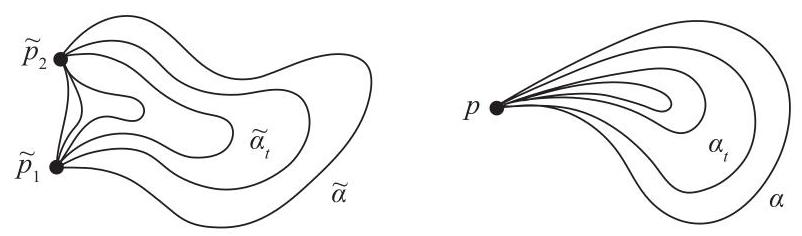
\includegraphics[max width=0.7\textwidth]{images/bo_d4b9jf3ef24c73e0334g_395_365_1805_802_236_0.jpg}
\end{center}
\hspace*{3em} 

图 5-26

为了使上述启发式论证严谨，我们必须定义“连接两个给定弧的连续弧族”，并证明这样的族可以被“提升”.

定义 2. 令 \(\mathrm{B} \subset  {\mathbb{R}}^{3}\) ，令 \({\alpha }_{0} : \left\lbrack  {0,l}\right\rbrack   \rightarrow  \mathrm{B},{\alpha }_{1} : \left\lbrack  {0,l}\right\rbrack   \rightarrow  \mathrm{B}\) 为 \(\mathrm{B}\) 的两条弧，连接点

\[
\mathrm{p} = {\alpha }_{0}\left( 0\right)  = {\alpha }_{1}\left( 0\right) \;\text{ and }\;\mathrm{q} = {\alpha }_{0}\left( l\right)  = {\alpha }_{1}\left( l\right) .
\]

我们称 \({\alpha }_{0}\) 和 \({\alpha }_{1}\) 是同伦的，如果存在一个连续映射 \(\mathrm{H} : \left\lbrack  {0,l}\right\rbrack   \times  \left\lbrack  {0,1}\right\rbrack   \rightarrow  \mathrm{B}\) 使得

1. \(\mathrm{H}\left( {S,0}\right)  = {\alpha }_{0}\left( \mathrm{\;s}\right) ,\mathrm{H}\left( {S,1}\right)  = {\alpha }_{1}\left( \mathrm{\;s}\right) ,\;S \in  \left\lbrack  {0,l}\right\rbrack\) .

2. \(\mathrm{H}\left( {0,\mathrm{t}}\right)  = \mathrm{p},\mathrm{H}\left( {l,\mathrm{t}}\right)  = \mathrm{q},\;\mathrm{t} \in  \left\lbrack  {0,1}\right\rbrack\) .

映射 \(\mathrm{H}\) 被称为 \({\alpha }_{0}\) 和 \({\alpha }_{1}\) 之间的同伦.

对于每一个 \(t \in  \left\lbrack  {0,1}\right\rbrack\) ，由 \({\alpha }_{t}\left( s\right)  = H\left( {s,t}\right)\) 给出的弧 \({\alpha }_{t} : \left\lbrack  {0,l}\right\rbrack   \rightarrow  B\) 被称为同伦 \(H\) 的一条弧.因此，同伦是一族弧 \({\alpha }_{t},t \in  \left\lbrack  {0,1}\right\rbrack\) ，它构成了 \({\alpha }_{0}\) 到 \({\alpha }_{1}\) 的连续变形(见图 5-27)，使得弧 \({\alpha }_{t}\) 的端点 \(p\) 和 \(q\) 在变形过程中保持固定(条件 2).

\begin{center}
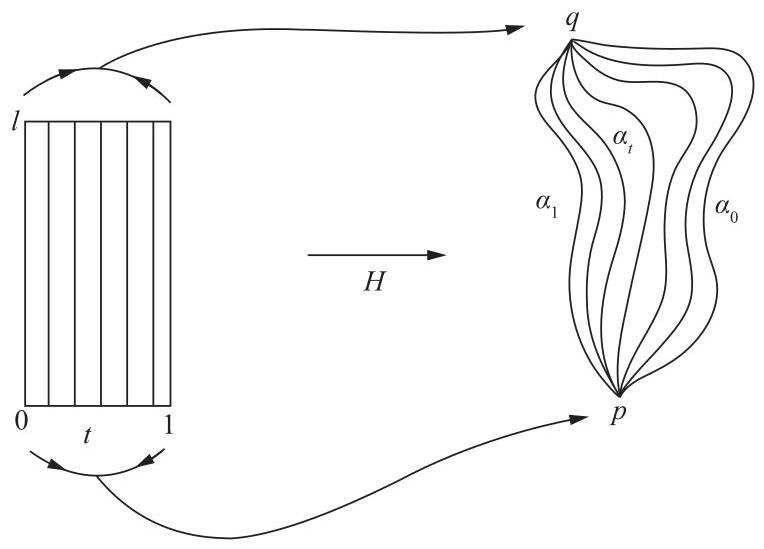
\includegraphics[max width=0.6\textwidth]{images/bo_d4b9jf3ef24c73e0334g_396_400_1087_764_549_0.jpg}
\end{center}
\hspace*{3em} 

图 5-27

同伦提升的概念与弧提升的概念完全类似.令 \(\pi  : \widetilde{B} \rightarrow  B\) 为一个连续映射，令 \({\alpha }_{0},{\alpha }_{1} : \left\lbrack  {0,l}\right\rbrack   \rightarrow  B\) 为连接点 \(p\) 和 \(q\) 的 \(B\) 的两条弧.令 \(H : \left\lbrack  {0,l}\right\rbrack   \times  \left\lbrack  {0,1}\right\rbrack   \rightarrow  B\) 为 \({\alpha }_{0}\) 和 \({\alpha }_{1}\) 之间的同伦.如果存在一个连续映射

\[
\widetilde{H} : \left\lbrack  {0,l}\right\rbrack   \times  \left\lbrack  {0,1}\right\rbrack   \rightarrow  \widetilde{B}
\]

使得 \(\pi  \circ  \widetilde{H} = H\) ，我们称 \(\widetilde{H}\) 是同伦 \(H\) 的提升，起点为 \(\widetilde{H}\left( {0,0}\right)  = \widetilde{p} \in  \widetilde{B}\) .

我们现在将证明覆盖映射具有提升同伦的性质.实际上，我们将证明一个更一般的命题.注意到覆盖映射 \(\pi  : \widetilde{B} \rightarrow  B\) 是一个局部同胚，并且，此外， \(B\) 的每一条弧都可以被提升为 \(\widetilde{B}\) 的一条弧.对于下面命题 3、4 和 5 的证明，我们将只使用覆盖映射的这两个性质，因此，为了将来使用，我们将以这种普遍性来陈述这些命题.因此，我们将说一个连续映射 \(\pi  : \widetilde{B} \rightarrow  B\) 具有提升弧的性质，当 \(B\) 的每一条弧都可以被提升时.注意到这蕴含了 \(\pi\) 将 \(\widetilde{B}\) 映射到 \(B\) .

命题 3. 设 \(B\) 是弧连通的，设 \(\pi  : \widetilde{\mathrm{B}} \rightarrow  \mathrm{B}\) 是具有提升弧性质的局部同胚. 设 \({\alpha }_{0},{\alpha }_{1} : \left\lbrack  {0,l}\right\rbrack   \rightarrow  B\) 是 \(\mathrm{B}\) 的两条连接点 \(\mathrm{p}\) 和 \(\mathrm{q}\) 的弧，设

\[
\text{ H: }\left\lbrack  {0,l}\right\rbrack   \times  \left\lbrack  {0,1}\right\rbrack   \rightarrow  \mathrm{B}
\]

是 \({\alpha }_{0}\) 和 \({\alpha }_{1}\) 之间的一个同伦，令 \(\widetilde{\mathrm{p}} \in  \widetilde{\mathrm{B}}\) 为 \(\widetilde{\mathrm{B}}\) 的一点，使得 \(\pi \left( \widetilde{\mathrm{p}}\right)  = \mathrm{p}\) .那么存在一个唯一的提升 \(\widetilde{\mathrm{H}}\) ，它是 \(\mathrm{H}\) 的，起点为 \(\widetilde{\mathrm{p}}\) .

证明. 唯一性的证明与弧的提升的证明完全类似. 设 \({\widetilde{H}}_{1}\) 和 \({\widetilde{H}}_{2}\) 是 \(H\) 的两个提升，具有 \({\widetilde{H}}_{1}\left( {0,0}\right)  = {\widetilde{H}}_{2}\left( {0,0}\right)  = \; \widetilde{p}\) . 则点集 \(A\) ，其中 \(\left( {s,t}\right)  \in  \left\lbrack  {0,l}\right\rbrack   \times  \left\lbrack  {0,1}\right\rbrack   = Q\) 使得 \({\widetilde{H}}_{1}\left( {s,t}\right)  = \; {\widetilde{H}}_{2}\left( {s,t}\right)\) ，非空且在 \(Q\) 中是闭集. 由于 \({\widetilde{H}}_{1}\) 和 \({\widetilde{H}}_{2}\) 是连续的，并且 \(\pi\) 是局部同胚，则 \(A\) 在 \(Q\) 中是开集. 由 \(Q,A = Q\) 的连通性；因此， \({\widetilde{H}}_{1} = {\widetilde{H}}_{2}\) .

为了证明存在性，设 \({\alpha }_{t}\left( s\right)  = H\left( {s,t}\right)\) 是同伦 \(H\) 的一条弧. 定义 \(\widetilde{H}\) 为

\[
\widetilde{H}\left( {s,t}\right)  = {\widetilde{\alpha }}_{t}\left( s\right) ,\;s \in  \left\lbrack  {0,l}\right\rbrack  ,t \in  \left\lbrack  {0,1}\right\rbrack  ,
\]

其中 \({\widetilde{\alpha }}_{t}\) 是 \({\alpha }_{t}\) 的提升，起点为 \(\widetilde{p}\) . 显然

\[
\pi  \circ  \widetilde{H}\left( {s,t}\right)  = {\alpha }_{t}\left( s\right)  = H\left( {s,t}\right) ,\;s \in  \left\lbrack  {0,l}\right\rbrack  ,t \in  \left\lbrack  {0,1}\right\rbrack  ,
\]

\[
\widetilde{H}\left( {0,0}\right)  = {\widetilde{\alpha }}_{0}\left( 0\right)  = \widetilde{p}.
\]

现在我们证明 \(\widetilde{H}\) 是连续的. 设 \(\left( {{s}_{0},{t}_{0}}\right)  \in  \left\lbrack  {0,l}\right\rbrack   \times  \left\lbrack  {0,1}\right\rbrack\) . 由于 \(\pi\) 是局部同胚，存在 \(\widetilde{H}\left( {{s}_{0},{t}_{0}}\right)\) 的一个邻域 \(V\) ，使得 \(\pi\) 在 \(V\) 上的限制 \({\pi }_{0}\) 是一个同胚，映射到一个 \(H\left( {{s}_{0},{t}_{0}}\right)\) 的邻域 \(U\) . 设 \({Q}_{0} \subset  {H}^{-1}\left( U\right)  \subset  \left\lbrack  {0,l}\right\rbrack   \times  \left\lbrack  {0,1}\right\rbrack\) 是一个由以下给出的开方块

\[
{S}_{0} - \epsilon  < S < {S}_{0} + \epsilon ,\;{t}_{0} - \epsilon  < t < {t}_{0} + \epsilon .
\]

只需证明 \(\widetilde{H}\) 在 \({Q}_{0}\) 上的限制可以写成 \(\widetilde{H} = {\pi }_{0}^{-1} \circ  H\) ，即可得出 \(\widetilde{H}\) 在 \(\left( {{s}_{0},{t}_{0}}\right)\) 处连续.由于 \(\left( {{s}_{0},{t}_{0}}\right)\) 是任意的， \(\widetilde{H}\) 在 \(\left\lbrack  {0,l}\right\rbrack   \times  \left\lbrack  {0,1}\right\rbrack\) 中是连续的，正如所愿.

为此，我们观察到

\[
{\pi }_{0}^{-1}\left( {H\left( {{s}_{0},t}\right) }\right) ,\;t \in  \left( {{t}_{0} - \epsilon ,{t}_{0} + \epsilon }\right) ,
\]

是穿过 \(\widetilde{H}\left( {{s}_{0},{t}_{0}}\right)\) 的弧 \(H\left( {{s}_{0},t}\right)\) 的提升.根据唯一性， \({\pi }_{0}^{-1}\left( {H\left( {{s}_{0},t}\right) }\right)  = \widetilde{H}\left( {{s}_{0},t}\right)\) .由于 \({Q}_{0}\) 是一个正方形，对于每一个 \(\left( {{s}_{1},{t}_{1}}\right)  \in  {Q}_{0}\) 都存在一个在 \(U,s \in  \left( {{s}_{0} - \epsilon ,{s}_{0} + \epsilon }\right)\) 中的弧 \(H\left( {s,{t}_{1}}\right)\) ，它与 \(\operatorname{arc}H\left( {{s}_{0},t}\right)\) 相交.由于 \({\pi }_{0}^{-1}\left( {H\left( {{s}_{0},{t}_{1}}\right) }\right)  = \widetilde{H}\left( {{s}_{0},{t}_{1}}\right)\) ， \(\operatorname{arc}{\pi }_{0}^{-1}\left( {H\left( {s,{t}_{1}}\right) }\right)\) 是穿过 \(\widetilde{H}\left( {{s}_{0},{t}_{1}}\right)\) 的弧 \(H\left( {s,{t}_{1}}\right)\) 的提升.根据提升的唯一性， \({\pi }_{0}^{-1}\left( {H\left( {s,{t}_{1}}\right) }\right)  = \widetilde{H}\left( {s,{t}_{1}}\right)\) ；因此， \({\pi }_{0}^{-1}\left( {H\left( {{s}_{1},{t}_{1}}\right) }\right)  = \widetilde{H}\left( {{s}_{1},{t}_{1}}\right)\) .通过 \(\left( {{s}_{1},{t}_{1}}\right)  \in  {Q}_{0}\) 的任意性，我们得出 \({\pi }_{0}^{-1}\left( {H\left( {s,t}\right) }\right)  = \widetilde{H}\left( {s,t}\right) ,\left( {s,t}\right)  \in  {Q}_{0}\) ，证明结束.Q.E.D.

命题 3 的一个推论是，如果 \(\pi  : \widetilde{B} \rightarrow  B\) 是一个覆盖映射，那么 \(B\) 的同伦弧会被提升为 \(\widetilde{B}\) 的同伦弧.这可以用一种更普遍、更精确的方式表达如下.

命题 4. 设 \(\pi  : \widetilde{\mathrm{B}} \rightarrow  \mathrm{B}\) 是一个具有弧提升性质的局部同胚. 设 \({\alpha }_{0},{\alpha }_{1} : \left\lbrack  {0,l}\right\rbrack   \rightarrow  \mathrm{B}\) 是 \(\mathrm{B}\) 中连接点 \(\mathrm{p}\) 和 \(\mathrm{q}\) 的两条弧, 并选择 \(\widetilde{\mathrm{p}} \in  \widetilde{\mathrm{B}}\) 使得 \(\pi \left( \widetilde{\mathrm{p}}\right)  = \mathrm{p}\) . 如果 \({\alpha }_{0}\) 和 \({\alpha }_{1}\) 同伦, 则以 \(\widetilde{\mathrm{p}}\) 为起点, \({\alpha }_{0}\) 和 \({\alpha }_{1}\) 的提升 \({\widetilde{\alpha }}_{0}\) 和 \({\widetilde{\alpha }}_{1}\) 也同伦.

证明. 设 \(H\) 是 \({\alpha }_{0}\) 和 \({\alpha }_{1}\) 之间的同伦, 设 \(\widetilde{H}\) 是其提升, 起点为 \(\widetilde{p}\) . 我们将证明 \(\widetilde{H}\) 是 \({\widetilde{\alpha }}_{0}\) 和 \({\widetilde{\alpha }}_{1}\) 之间的同伦 (参见图 5-28).

\begin{center}
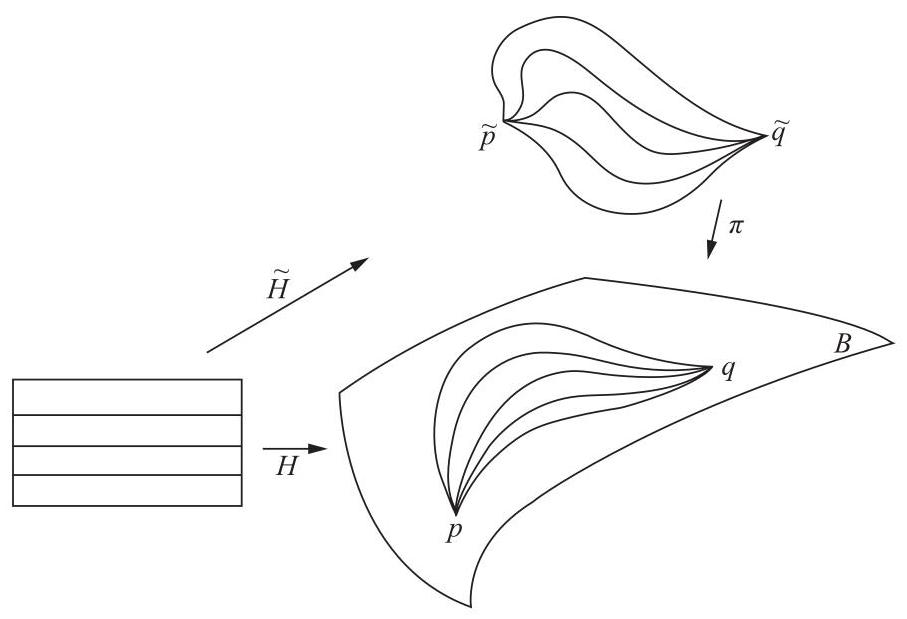
\includegraphics[max width=0.8\textwidth]{images/bo_d4b9jf3ef24c73e0334g_398_330_1425_907_619_0.jpg}
\end{center}
\hspace*{3em} 

图 5-28

事实上, 根据弧提升的唯一性,

\[
\widetilde{H}\left( {s,0}\right)  = {\widetilde{\alpha }}_{0}\left( s\right) ,\;\widetilde{H}\left( {s,1}\right)  = {\widetilde{\alpha }}_{1}\left( s\right) ,\;s \in  \left\lbrack  {0,l}\right\rbrack  ,
\]

这验证了定义 2 的条件 1. 此外, \(\widetilde{H}\left( {0,t}\right)\) 是以 \(\widetilde{p}\) 为起点, "常值"弧 \(H\left( {0,t}\right)  = p\) 的提升. 根据唯一性,

\[
\widetilde{H}\left( {0,t}\right)  = \widetilde{p},\;t \in  \left\lbrack  {0,1}\right\rbrack  .
\]

类似地， \(\widetilde{H}\left( {l,t}\right)\) 是 \(H\left( {l,t}\right)  = q\) 的提升，其起点为 \({\widetilde{\alpha }}_{0}\left( l\right)  = \widetilde{q}\) ；因此，

\[
\widetilde{H}\left( {l,t}\right)  = \widetilde{q} = {\alpha }_{1}\left( l\right) ,\;t \in  \left\lbrack  {0,1}\right\rbrack  .
\]

因此，定义 2 的条件 2 得到验证，表明 \(\widetilde{H}\) 是 \({\widetilde{\alpha }}_{0}\) 和 \({\widetilde{\alpha }}_{1}\) 之间的同伦.Q.E.D.

回到引导我们考虑同伦概念的启发式论证，我们看到仍然需要解释“没有‘洞’的空间”是什么意思.当然，我们将把启发式论证中使用的性质作为这种空间的定义.

定义 3. 一个弧状连通集 \(\mathrm{B} \subset  {\mathbb{R}}^{3}\) 是单连通的，如果给定两点 \(\mathrm{p},\mathrm{q} \in  \mathrm{B}\) 和连接 \(\mathrm{p}\) 到 \(\mathrm{q}\) 的两条弧 \({\alpha }_{0} : \left\lbrack  {0,l}\right\rbrack   \rightarrow  \mathrm{B},{\alpha }_{1} : \left\lbrack  {0,l}\right\rbrack   \rightarrow  \mathrm{B}\) ，在 \(\mathrm{B}\) 中存在一条连接 \({\alpha }_{0}\) 和 \({\alpha }_{1}\) 的同伦.特别地， \(\mathrm{B},\alpha  : \left\lbrack  {0,l}\right\rbrack   \rightarrow  \mathrm{B}\) 的任何闭合弧(闭合意味着 \(\alpha \left( 0\right)  = \alpha \left( l\right)  = \mathrm{p}\) )都与“常数”弧 \(\alpha \left( S\right)  = \mathrm{p},S \in  \left\lbrack  {0,l}\right\rbrack\) 同伦(练习 5 表明最后一个性质实际上等同于第一个性质).

直观地说，一个弧状连通集 \(B\) 是单连通的，如果 \(B\) 中的每条闭合弧都可以连续地变形为一点.可以证明平面和球面是单连通的，而圆柱体和环面不是单连通的(参见练习 5).

现在我们可以陈述并证明本节问题 2 的答案.这将是以下命题的一个推论.

命题 5. 设 \(\pi  : \widetilde{\mathrm{B}} \rightarrow  \mathrm{B}\) 是一个具有弧提升性质的局部同胚.设 \(\widetilde{\mathrm{B}}\) 是弧状连通的， \(\mathrm{B}\) 是单连通的.则 \(\pi\) 是一个同胚.

证明. 证明与启发式论证中提出的基本相同.

我们需要证明 \(\pi\) 是单射的.为此，设 \({\widetilde{p}}_{1}\) 和 \({\widetilde{p}}_{2}\) 是 \(\widetilde{B}\) 的两个点，且 \(\pi \left( {\widetilde{p}}_{1}\right)  = \pi \left( {\widetilde{p}}_{2}\right)  = p\) .由于 \(\widetilde{B}\) 是弧连通的，存在一条连接 \({\widetilde{p}}_{1}\) 和 \({\widetilde{p}}_{2}\) 的 \(\widetilde{B}\) 的弧 \({\widetilde{\alpha }}_{0}\) .那么 \(\pi  \circ  {\widetilde{\alpha }}_{0} = {\alpha }_{0}\) 是 \(B\) 的一个闭弧.由于 \(B\) 是单连通的， \({\alpha }_{0}\) 与常弧 \({\alpha }_{1}\left( s\right)  = p,s \in  \left\lbrack  {0,l}\right\rbrack\) 同伦.根据命题 4， \({\widetilde{\alpha }}_{0}\) 与以 \(p\) 为起点的 \({\alpha }_{1}\) 的提升 \({\widetilde{\alpha }}_{1}\) 同伦.

由于 \({\widetilde{\alpha }}_{1}\) 是连接点 \({\widetilde{p}}_{1}\) 和 \({\widetilde{p}}_{2}\) 的常弧，我们得出 \({\widetilde{p}}_{1} = {\widetilde{p}}_{2}.\) .证毕.

推论.设 \(\pi  : \widetilde{\mathrm{B}} \rightarrow  \mathrm{B}\) 是一个覆盖映射， \(\widetilde{\mathrm{B}}\) 弧连通， \(\mathrm{B}\) 单连通.则 \(\pi\) 是一个同胚.

我们证明命题 3、4 和 5 时具有比严格必需的更一般的性质这一事实，将使我们能够对问题 1 给出另一个答案，如下所述.

设 \(\pi  : \widetilde{B} \rightarrow  B\) 是一个具有提升弧性质的局部同胚，并假设 \(\widetilde{B}\) 和 \(B\) 在局部是“良好的”(待精确定义).则 \(\pi\) 实际上是一个覆盖映射.

所需的局部性质描述如下.回想一下，如果每个点的邻域都包含一个弧连通的邻域，则 \(B \subset  {R}^{3}\) 是局部弧连通的(第 5 章附录，定义 12).

定义 4.如果每个点的邻域都包含一个单连通的邻域，则 B 是局部单连通的.

换句话说，如果每个点都有任意小的单连通邻域，则 \(B\) 是局部单连通的.显然，如果 \(B\) 是局部单连通的，那么 \(B\) 是局部弧连通的.

我们注意到，一个正则曲面 \(S\) 是局部单连通的，因为 \(p \in  S\) 有任意小的邻域同胚于平面圆盘的内部.

在下一个命题中，我们将需要一个局部弧连通集 \(B \subset  {R}^{3}\) 的以下性质(参见第 5 章附录，D 部分).包含点 \(p \in  B\) 的所有弧连通子集的并集显然是一个弧连通集 \(A\) ，该集被称为包含 \(p\) 的 \(B\) 的弧连通分量.由于 \(B\) 是局部弧连通的， \(A\) 在 \(B\) 中是开集.因此， \(B\) 可以写成其开的、两两不相交的连通分量 \({A}_{\alpha }\) 的并集 \(B = \mathop{\bigcup }\limits_{\alpha }{A}_{\alpha }\) .

我们还注意到，一个正则曲面是局部弧连通的.因此，在下面的命题中，当 \(B\) 和 \(\widetilde{B}\) 都是正则曲面时，关于 \(B\) 和 \(\widetilde{B}\) 的假设就满足了.

命题 6. 设 \(\pi  : \widetilde{\mathrm{B}} \rightarrow  \mathrm{B}\) 是一个具有弧提升性质的局部同胚映射.假设 \(\mathrm{B}\) 是局部单连通的，而 \(\widetilde{\mathrm{B}}\) 是局部弧连通的.则 \(\pi\) 是一个覆盖映射.

证明. 设 \(p \in  B\) 且设 \(V\) 是 \(B\) 中 \(p\) 的一个单连通邻域.集合 \({\pi }^{-1}\left( V\right)\) 是其弧连通分量的并集；即，

\[
{\pi }^{-1}\left( V\right)  = \mathop{\bigcup }\limits_{\alpha }{\widetilde{V}}_{\alpha }
\]

其中 \({\widetilde{V}}_{\alpha }\) 是开集、弧连通且两两不相交的集合.考虑限制 \(\pi  : {\widetilde{V}}_{\alpha } \rightarrow  V\) .如果我们证明 \(\pi\) 是 \({\widetilde{V}}_{\alpha }\) 到 \(V,\pi\) 的一个同胚映射，则满足覆盖映射定义的条件.

我们首先证明 \(\pi \left( {\widetilde{V}}_{\alpha }\right)  = V\) .事实上， \(\pi \left( {\widetilde{V}}_{\alpha }\right)  \subset  V\) .假设存在一点 \(p \in  V,p \notin  \pi \left( {\widetilde{V}}_{\alpha }\right)\) .那么，由于 \(V\) 是弧连通的，存在一个连接点 \(q \in  \pi \left( {\widetilde{V}}_{\alpha }\right)\) 和 \(p\) 的 \(\operatorname{arc}\alpha  : \left\lbrack  {a,b}\right\rbrack   \rightarrow  V\) .以 \(\widetilde{q} \in  {\widetilde{V}}_{\alpha }\) 为原点的 \(\alpha\) 的提升 \(\widetilde{\alpha } : \left\lbrack  {a,b}\right\rbrack   \rightarrow  \widetilde{B}\) ，其中 \(\pi \left( \widetilde{q}\right)  = q\) ，是在 \({\widetilde{V}}_{\alpha }\) 中的一条弧，因为 \({\widetilde{V}}_{\alpha }\) 是 \(B\) 的一个弧连通分量.因此，

\[
\pi \left( {\widetilde{\alpha }\left( b\right) }\right)  = p \in  \pi \left( {\widetilde{V}}_{\alpha }\right) ,
\]

这是一个矛盾，表明 \(\pi \left( {\widetilde{V}}_{\alpha }\right)  = V\) .

接下来，我们观察到 \(\pi  : {\widetilde{V}}_{\alpha } \rightarrow  V\) 仍然是一个局部同胚映射，因为 \({\widetilde{V}}_{\alpha }\) 是开集.此外，根据上述，映射 \(\pi  : {\widetilde{V}}_{\alpha } \rightarrow  V\) 仍然具有弧提升的性质.因此，我们已经满足了命题 5 的条件；因此， \(\pi\) 是一个同胚映射.证毕.

\section*{B. Hadamard 定理}

现在我们回到本节开头提出的问题，即在什么条件下，局部微分同胚 \({\exp }_{p} : {T}_{p}\left( S\right)  \rightarrow  S\) ，其中 \(p\) 是曲率为 \(K \leq  0\) 的完备曲面 \(S\) 的一个点，是 \({T}_{p}\left( S\right)\) 到 \(S\) 的全局微分同胚.以下命题将给定问题分解为问题 1 和问题 2，从而给出了问题的答案.

我们将需要以下引理.

引理 1. 设 \(S\) 是曲率为 \(\mathrm{K} \leq  0\) 的完备曲面.则 \({\exp }_{\mathrm{p}} : {\mathrm{T}}_{\mathrm{p}}\left( S\right)  \rightarrow  S,\mathrm{p} \in  S\) 在以下意义上是长度增加的:如果 \(\mathrm{u}\) ， \(\mathrm{w} \in  {\mathrm{T}}_{\mathrm{p}}\left( S\right)\) ，我们有

\[
\left\langle  {{\left( \mathrm{d}{\exp }_{\mathrm{p}}\right) }_{\mathrm{u}}\left( \mathrm{w}\right) ,{\left( \mathrm{d}{\exp }_{\mathrm{p}}\right) }_{\mathrm{u}}\left( \mathrm{w}\right) }\right\rangle   \geq  \langle \mathrm{w},\mathrm{w}\rangle ,
\]

其中，一如既往， \(\mathrm{w}\) 表示 \({\left( {\mathrm{T}}_{\mathrm{p}}\left( S\right) \right) }_{\mathrm{u}}\) 中的一个向量，该向量通过平移 u 从 \(\mathrm{w}\) 获得.

证明.对于情况 \(u = 0\) ，等式可平凡验证.因此，设 \(v = \; u/\left| u\right| ,u \neq  0\) ，并设 \(\gamma  : \left\lbrack  {0,l}\right\rbrack   \rightarrow  S,l = \left| u\right|\) 为测地线

\[
\gamma \left( s\right)  = {\exp }_{p}{sv},\;s \in  \left\lbrack  {0,l}\right\rbrack
\]

根据高斯引理，我们可以假设 \(\langle w,v\rangle  = 0\) .设 \(J\left( s\right)  = \; s{\left( d{\exp }_{p}\right) }_{sv}\left( w\right)\) 为 \(\gamma\) 沿引理 1，节 5-5 中的雅可比场.我们知道 \(J\left( 0\right)  = 0,\left( {{DJ}/{ds}}\right) \left( 0\right)  = w\) 和 \(\left\langle  {J\left( s\right) ,{\gamma }^{\prime }\left( s\right) }\right\rangle   = 0,s \in  \left\lbrack  {0,l}\right\rbrack\) .

现在注意到，由于 \(K \leq  0\) (参见方程 (1)，节 5-5)，

\[
\frac{d}{ds}\left\langle  {J,\frac{DJ}{ds}}\right\rangle   = \left\langle  {\frac{DJ}{ds},\frac{DJ}{ds}}\right\rangle   + \left\langle  {J,\frac{{D}^{2}J}{d{s}^{2}}}\right\rangle   = {\left| \frac{DJ}{ds}\right| }^{2} - K{\left| J\right| }^{2} \geq  0.
\]

这表明

\[
\left\langle  {J,\frac{DJ}{ds}}\right\rangle   \geq  0
\]

因此，

\[
\frac{d}{ds}\left\langle  {\frac{DJ}{ds},\frac{DJ}{ds}}\right\rangle   = 2\left\langle  {\frac{DJ}{ds},\frac{{D}^{2}J}{d{s}^{2}}}\right\rangle   =  - {2K}\left\langle  {\frac{DJ}{ds},J}\right\rangle   \geq  0. \tag{1}
\]

由此可知

\[
\left\langle  {\frac{DJ}{ds},\frac{DJ}{ds}}\right\rangle   \geq  \left\langle  {\frac{DJ}{ds}\left( 0\right) ,\frac{DJ}{ds}\left( 0\right) }\right\rangle   = \langle w,w\rangle  = C; \tag{2}
\]

因此，

\[
\frac{{d}^{2}}{d{s}^{2}}\langle J,J\rangle  = 2\left\langle  {\frac{DJ}{ds},\frac{DJ}{ds}}\right\rangle   + 2\left\langle  {J,\frac{{D}^{2}J}{d{s}^{2}}}\right\rangle   \geq  2\left\langle  {\frac{DJ}{ds},\frac{DJ}{ds}}\right\rangle   \geq  {2C}. \tag{3}
\]

通过对上述不等式两边积分，我们得到

\[
\frac{d}{ds}\langle J,J\rangle  \geq  {2Cs} + {\left( \frac{d}{ds}\langle J,J\rangle \right) }_{s = 0} = {2Cs} + 2\left\langle  {\frac{DJ}{ds}\left( 0\right) ,J\left( 0\right) }\right\rangle   = {2Cs}.
\]

再次积分得到

\[
\langle J,J\rangle  \geq  C{s}^{2} + \langle J\left( 0\right) ,J\left( 0\right) \rangle  = C{s}^{2}.
\]

通过在上述表达式中设置 \(s = l\) 并注意到 \(C = \langle w,w\rangle\) ，我们得到

\[
\langle J\left( l\right) ,J\left( l\right) \rangle  \geq  {l}^{2}\langle w,w\rangle .
\]

由于 \(J\left( l\right)  = l{\left( d{\exp }_{p}\right) }_{lv}\left( w\right)\) ，我们最终得出结论:

\[
\left\langle  {{\left( d{\exp }_{p}\right) }_{lv}\left( w\right) ,{\left( d\exp \right) }_{lv}\left( w\right) }\right\rangle   \geq  \langle w,w\rangle . \tag{Q.E.D.}
\]

为了以后使用，建立上述证明的以下推论是方便的.

推论(证明的推论).设 \(\mathrm{K} \equiv  0\) .则 \({\exp }_{\mathrm{p}} : {\mathrm{T}}_{\mathrm{p}}\left( S\right)  \rightarrow  S,\mathrm{p} \in  S\) 是一个局部等距映射.

只需注意到，如果 \(K \equiv  0\) ，则可以在上述证明的方程 (1)、(2) 和 (3) 中将“ \(\geq  0\) ”替换为“≡0”.

命题 7.设 \(S\) 是一个具有高斯曲率 \(\mathrm{K} \leq  0\) 的完备曲面.则映射 \({\exp }_{\mathrm{p}} : {\mathrm{T}}_{\mathrm{p}}\left( S\right)  \rightarrow  S,\mathrm{p} \in  S\) 是一个覆盖映射.

证明. 因为我们知道 \({\exp }_{p}\) 是一个局部微分同胚，所以(根据命题 6)只需证明 \({\exp }_{p}\) 具有提升弧的性质即可.

设 \(\alpha  : \left\lbrack  {0,l}\right\rbrack   \rightarrow  S\) 是 \(S\) 中的一条弧，也设 \(v \in  {T}_{p}\left( S\right)\) 使得 \({\exp }_{p}v = \alpha \left( 0\right)\) . 这样的 \(v\) 存在，因为 \(S\) 是完备的. 因为 \({\exp }_{p}\) 是一个局部微分同胚，在 \({T}_{p}\left( S\right)\) 中存在 \(v\) 的一个邻域 \(U\) ，使得 \({\exp }_{p}\) 在 \(U\) 上的限制是一个微分同胚. 通过在 \({\exp }_{p}\left( U\right)\) 中使用 \({\exp }_{p}^{-1}\) ，可以在 0 的一个邻域中定义 \(\widetilde{\alpha }\) .

设 \(A\) 为满足 \(\widetilde{\alpha }\) 在 \(\left\lbrack  {0,t}\right\rbrack  .A\) 中定义且非空的 \(t \in  \left\lbrack  {0,l}\right\rbrack\) 的集合，并且如果 \(\widetilde{\alpha }\left( {t}_{0}\right)\) 已定义，则 \(\widetilde{\alpha }\) 在 \({t}_{0}\) 的邻域中定义；也就是说， \(A\) 在 \(\left\lbrack  {0,l}\right\rbrack\) 中是开集.一旦我们证明 \(A\) 在 \(\left\lbrack  {0,l}\right\rbrack\) 中是闭集，那么根据 \(\left\lbrack  {0,l}\right\rbrack\) 的连通性， \(A = \left\lbrack  {0,l}\right\rbrack\) 和 \(\alpha\) 就可以完全提升.

因此，证明的关键在于表明 \(A\) 在 \(\left\lbrack  {0,l}\right\rbrack\) 中是闭集. 为此，设 \({t}_{0} \in  \left\lbrack  {0,l}\right\rbrack\) 是 \(A\) 的一个聚点，设 \(\left\{  {t}_{n}\right\}\) 是一个序列，其中 \(\left\{  {t}_{n}\right\}   \rightarrow  {t}_{0},{t}_{n} \in  A,n = 1,2,\ldots\) . 我们将首先证明 \(\widetilde{\alpha }\left( {t}_{n}\right)\) 有一个聚点.

假设 \(\widetilde{\alpha }\left( {t}_{n}\right)\) 在 \({T}_{p}\left( S\right)\) 中没有聚点. 那么，给定 \({T}_{p}\left( S\right)\) 中的一个闭圆盘 \(D\) ，其圆心为 \(\widetilde{\alpha }\left( 0\right)\) ，存在一个 \({n}_{0}\) 使得 \(\widetilde{\alpha }\left( {t}_{{n}_{0}}\right)  \notin  D\) . 因此，在 \({T}_{p}\left( S\right)\) 中，从 \(\widetilde{\alpha }\left( 0\right)\) 到 \(\widetilde{\alpha }\left( {t}_{n}\right)\) 的距离任意大. 因为根据引理 1， \({\exp }_{p} : {T}_{p}\left( S\right)  \rightarrow  S\) 增加了向量的长度，我们得到，通过将 \(d\) 设置为 \({T}_{p}\left( S\right)\) 中的距离，

\[
{l}_{\left\lbrack  0,{t}_{n}\right\rbrack  } = {\int }_{0}^{{t}_{n}}\left| {{\alpha }^{\prime }\left( t\right) }\right| {dt} = {\int }_{0}^{{t}_{n}}\left| {d{\exp }_{p}\left( {\widetilde{\alpha }}^{\prime }\right) }\right| {dt}
\]

\[
\geq  {\int }_{0}^{{t}_{n}}\left| {{\widetilde{\alpha }}^{\prime }\left( t\right) }\right| {dt} = d\left( {\widetilde{\alpha }\left( 0\right) ,\widetilde{\alpha }\left( {t}_{n}\right) }\right) .
\]

这表明 0 和 \({t}_{n}\) 之间 \(\alpha\) 的长度任意大，这是一个矛盾，证明了该断言.

我们将用 \(q\) 表示 \(\widetilde{\alpha }\left( {t}_{n}\right)\) 的一个聚点.

令 \(V\) 为 \({T}_{p}\left( S\right)\) 中的 \(q\) 的一个邻域，使得 \({\exp }_{p}\) 在 \(V\) 上的限制是一个微分同胚.由于 \(q\) 是 \(\left\{  {\widetilde{\alpha }\left( {t}_{n}\right) }\right\}\) 的一个聚点，存在一个 \({n}_{1}\) 使得 \(\widetilde{\alpha }\left( {t}_{{n}_{1}}\right)  \in  V\) .此外，由于 \(\alpha\) 是连续的，存在一个开区间 \(I \subset  \left\lbrack  {0,l}\right\rbrack  ,{t}_{0} \subset  I\) ，使得 \(\alpha \left( I\right)  \subset  {\exp }_{p}\left( V\right)  = U\) .通过使用 \(U\) 中 \({\exp }_{p}^{-1}\) 的限制，可以在 \(I\) 中定义 \(\alpha\) 的一个提升，其起点为 \(\widetilde{\alpha }\left( {t}_{{n}_{1}}\right)\) .由于 \({\exp }_{p}\) 是一个局部微分同胚，这个提升在 \(\left\lbrack  {0,{t}_{0}}\right)  \cap  I\) 中与 \(\widetilde{\alpha }\) 重合，因此是 \(\widetilde{\alpha }\) 到包含 \({t}_{0}\) 的一个区间的延拓.因此，集合 \(A\) 是闭合的，这结束了命题 7 的证明.

Q.E.D.

注记 1.应该注意到，曲率条件 \(K \leq  0\) 仅用于保证 \({\exp }_{p} : {T}_{p}\left( S\right)  \rightarrow  S\) 是一个长度增大的局部微分同胚.因此，我们实际上证明了，如果 \(\varphi  : {S}_{1} \rightarrow  {S}_{2}\) 是一个完备曲面 \({S}_{1}\) 到曲面 \({S}_{2}\) 的局部微分同胚，并且是长度增大的，那么 \(\varphi\) 是一个覆盖映射.

以下命题，即 Hadamard 定理，描述了具有曲率 \(K \leq  0\) 的完备曲面的拓扑结构.

定理 1 (Hadamard).设 \(S\) 是一个单连通的完备曲面，其高斯曲率为 \(\mathrm{K} \leq  0\) .那么 \({\exp }_{\mathrm{p}} : {\mathrm{T}}_{\mathrm{p}}\left( S\right)  \rightarrow  S,\mathrm{p} \in  S\) 是一个微分同胚；也就是说， \(S\) 与一个平面微分同胚.

证明.根据命题 7， \({\exp }_{p} : {T}_{p}\left( S\right)  \rightarrow  S\) 是一个覆盖映射.根据命题 5 的推论， \({\exp }_{p}\) 是一个同胚.由于 \({\exp }_{p}\) 是一个局部微分同胚，其逆映射是可微的，并且 \({\exp }_{p}\) 是一个微分同胚.

我们现在将介绍覆盖空间又一个几何应用，也称为 Hadamard 定理.回顾一个连通的、紧致的、正则曲面，其高斯曲率为 \(K > 0\) ，称为卵形面(参见注记 2，第 5-2 节).

定理 2 (Hadamard).设 S 是一个卵形面.那么高斯映射 \(N : S \rightarrow  {S}^{2}\) 是一个微分同胚.特别地， \(S\) 与一个球面微分同胚.

证明.由于对于每个 \(p \in  S\) ， \(S,K = \det \left( {d{N}_{p}}\right)\) 的高斯曲率为正，所以 \(N\) 是局部微分同胚.根据命题 1， \(N\) 是覆盖映射.由于球面 \({S}^{2}\) 是单连通的，我们从命题 5 的推论得出， \(N : S \rightarrow  {S}^{2}\) 是 \(S\) 到单位球面 \({S}^{2}\) 的同胚.由于 \(N\) 是局部微分同胚，其逆映射是可微的.因此， \(N\) 是微分同胚.证毕.

注 2. 实际上，我们证明了更多内容. 由于高斯映射 \(N\) 是一个微分同胚， \({R}^{3}\) 的每一个单位向量 \(v\) 都恰好作为 \(S\) 的一个单位法向量出现一次. 取一个垂直于 \(v\) 且远离表面的平面，并将其平行移动直到它与表面相交，我们得出 \(S\) 位于其每个切平面的同一侧. 这被表述为卵形面 \(S\) 是局部凸的. 由此可以证明 \(S\) 实际上是一个凸集(即，集合 \(K \subset  {R}^{3}\) 使得连接任意两点 \(p,q \in  K\) 的线段完全属于 \(K\) )的边界.

注 3. 具有 \(K > 0\) 的紧致曲面同胚于球面这一事实已被 S. S. Chern 和 R. K. Lashof 推广到具有 \(K \geq  0\) 的紧致曲面(“On the Total Curvature of Immersed Manifolds,” Michigan Math. J. 5 (1958), 5-12). J. J. Stoker 最早获得了完整曲面的推广(“Über die Gestalt der positiv gekrümnten offenen

Fläche,” Compositio Math. 3 (1936), 58-89)，他证明了，除其他外，以下结论:具有 \(K > 0\) 的完整曲面同胚于球面或平面. 如果假设在某一点 \(K > 0\) (有关证明和该问题的调查，请参阅 M. do Carmo 和 E. Lima，“Isometric Immersions with Non-negative Sectional Curvatures,” Boletim da Soc. Bras. Mat. 2 (1971), 9-22)，则该结果对于 \(K \geq  0\) 仍然成立.

\exerciseline

1. 证明由 \(\pi \left( t\right)  = \left( {\cos t,\sin t}\right) ,t \in  R\) 给出的映射 \(\pi  : R \rightarrow  {S}^{1} = \left\{  {\left( {x,y}\right)  \in  {R}^{2};{x}^{2} + {y}^{2} = 1}\right\}\) 是一个覆盖映射.

2. 证明由 \(\pi  : {R}^{2} - \{ 0,0\}  \rightarrow  {R}^{2} - \{ 0,0\}\) 给出的映射是

\[
\pi \left( {x,y}\right)  = \left( {{x}^{2} - {y}^{2},{2xy}}\right) ,\;\left( {x,y}\right)  \in  {R}^{2},
\]

一个双层覆盖映射.

3. 令 \(S\) 为由螺旋线( \(\cos t,\sin t,{bt}\) )的法线生成的螺旋面. 令 \(L\) 为 \(z\) 轴，令 \(\pi  : S - L \rightarrow  {R}^{2} - \{ 0,0\}\) 为投影 \(\pi \left( {x,y,z}\right)  = \left( {x,y}\right)\) . 证明 \(\pi\) 是一个覆盖映射.

4. 熟悉复变函数的人会注意到，练习2中的映射 \(\pi\) 正是从 \(\mathbb{C} - \{ 0\}\) 到 \(\mathbb{C} - \{ 0\}\) 的映射 \(\pi \left( z\right)  = {z}^{2}\) ；这里 \(\mathbb{C}\) 是复平面，而 \(z \in  \mathbb{C}\) .通过证明映射 \(\pi  : \mathbb{C} - \{ 0\}  \rightarrow  \mathbb{C} - \{ 0\}\) 由 \(\pi \left( z\right)  = {z}^{n}\) 给出是一个 \(n\) 重覆盖映射，来推广这一结论.

5. 令 \(B \subset  {R}^{3}\) 为一个弧连通集.证明以下两个性质是等价的(参见定义3):

1. 对于任意两点 \(p,q \in  B\) 以及任意两条弧 \({\alpha }_{0} : \left\lbrack  {0,l}\right\rbrack   \rightarrow  B\) ， \({\alpha }_{1} : \left\lbrack  {0,l}\right\rbrack   \rightarrow  B\) ，存在一个在 \(B\) 中的同伦连接 \({\alpha }_{0}\) 到 \({\alpha }_{1}\) .

2. 对于任意 \(p \in  B\) 以及任意弧 \(\alpha  : \left\lbrack  {0,l}\right\rbrack   \rightarrow  B\) ，其中 \(\alpha \left( 0\right)  = \alpha \left( l\right)  = p\) (即 \(\alpha\) 是一条首尾点为 \(p\) 的闭合弧)，存在一个同伦连接 \(\alpha\) 到常数弧 \(\alpha \left( s\right)  = p,s \in  \left\lbrack  {0,l}\right\rbrack\) .

6. 固定一点 \({p}_{0} \in  {R}^{2}\) ，定义一个映射族 \({\varphi }_{t} : {R}^{2} \rightarrow  {R}^{2},t \in  \left\lbrack  {0,1}\right\rbrack\) ，由 \({\varphi }_{t}\left( p\right)  = t{p}_{0} + \left( {1 - t}\right) p,p \in  {R}^{2}\) 给出.注意到 \({\varphi }_{0}\left( p\right)  = p,{\varphi }_{1}\left( p\right)  = {p}_{0}\) .因此， \({\varphi }_{t}\) 是一个连续的映射族，它从恒等映射开始，以常数映射 \({p}_{0}\) 结束.应用这些考虑来证明 \({R}^{2}\) 是单连通的.

7. a. 使用球极投影和练习6来证明，球面 \({S}^{2}\) 上任何省略了至少一点的闭合弧都与一条常数弧同伦.

b. 证明球面 \({S}^{2}\) 上的任何闭合弧都与一条省略了至少一点的 \({S}^{2}\) 中的闭合弧同伦.

c. 从a和b部分得出结论， \({S}^{2}\) 是单连通的.为什么b部分是必需的？

8. (克林根贝格引理.)设 \(S \subset  {R}^{3}\) 为一个完备曲面，其高斯曲率为 \(K \leq  {K}_{0}\) ，其中 \({K}_{0}\) 为非负常数.设 \(p,q \in  S\) ，且设 \({\gamma }_{0}\) 和 \({\gamma }_{1}\) 为连接 \(p\) 到 \(q\) 的两条不同的测地线，其中 \(l\left( {\gamma }_{0}\right)  \leq  l\left( {\gamma }_{1}\right)\) ；这里 \(l\) ( ) 表示相应曲线的长度.假设 \({\gamma }_{0}\) 同伦于 \({\gamma }_{1}\) ；即存在一个连续曲线族 \({\alpha }_{t}\) ， \(t \in  \left\lbrack  {0,1}\right\rbrack\) ，连接 \(p\) 到 \(q\) ，且 \({\alpha }_{0} = {\gamma }_{0},{\alpha }_{1} = {\gamma }_{1}\) .本练习的目的是证明存在一个 \({t}_{0} \in  \left\lbrack  {0,1}\right\rbrack\) ，使得

\[
l\left( {\gamma }_{0}\right)  + l\left( {\alpha }_{{t}_{0}}\right)  \geq  \frac{2\pi }{\sqrt{{K}_{0}}}.
\]

(因此，同伦必须经过一条“长”曲线.见图 5-29.)假设 \(l\left( {\gamma }_{0}\right)  < \pi /\sqrt{{K}_{0}}\) (否则无需证明)，并按以下步骤进行.

\begin{center}
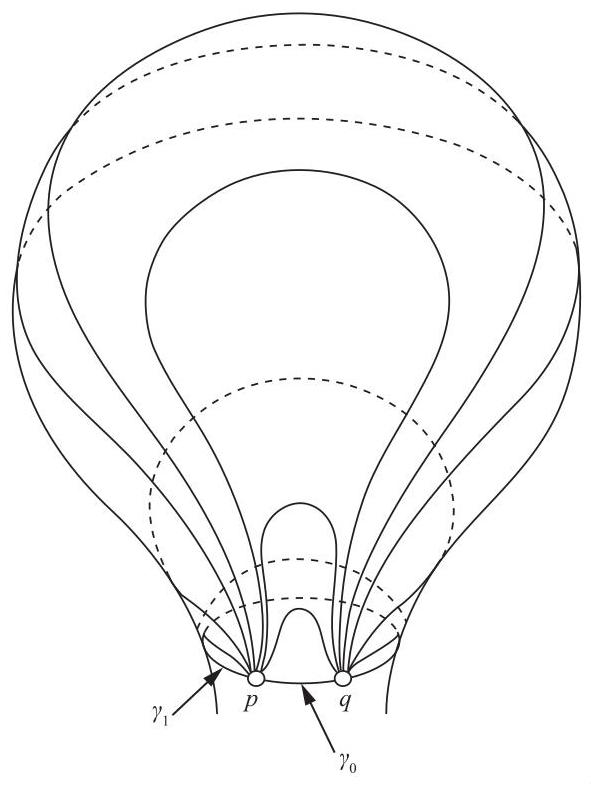
\includegraphics[max width=0.5\textwidth]{images/bo_d4b9jf3ef24c73e0334g_406_218_974_591_792_0.jpg}
\end{center}
\hspace*{3em} 

图 5-29. 克林根贝格引理.

a. 使用第一个比较定理 (参见练习 3，第 5-5 节) 证明 \({\exp }_{p} : {T}_{p}\left( S\right)  \rightarrow  S\) 在以 \(p\) 为中心、半径为 \(\pi /\sqrt{{K}_{0}}\) 的开圆盘 \(B\) 中没有临界点.

b. 证明，当 \(t\) 很小时，可以将曲线 \({\alpha }_{t}\) 提升到切平面 \({T}_{p}\left( S\right)\) 中；即存在一条曲线 \({\widetilde{\alpha }}_{t}\) 连接 \({\exp }_{p}^{-1}\left( p\right)  = 0\) 到 \({\exp }_{p}^{-1}\left( q\right)  = \widetilde{q}\) ，并且 \({\exp }_{p} \circ  {\widetilde{\alpha }}_{t} = {\alpha }_{t}\) .

c. 证明第 \(\mathrm{b}\) 部分的提升不能对所有 \(t \in  \left\lbrack  {0,1}\right\rbrack\) 定义.由此得出，对于每一个 \(\epsilon  > 0\) 都存在一个 \(t\left( \epsilon \right)\) ，使得 \({\alpha }_{t\left( \epsilon \right) }\) 可以被提升到 \({\widetilde{\alpha }}_{t\left( \epsilon \right) }\) 中，并且 \({\widetilde{\alpha }}_{t\left( \epsilon \right) }\) 包含距离 \(B\) 边界 \(< \epsilon\) 的点.因此，

\[
l\left( {\gamma }_{0}\right)  + l\left( {\alpha }_{t\left( \epsilon \right) }\right)  \geq  \frac{2\pi }{\sqrt{{K}_{0}}} - {2\epsilon }.
\]

d. 在第 \(\mathrm{c}\) 部分中选择一个 \({\epsilon }^{\prime }s,\left\{  {\epsilon }_{n}\right\}   \rightarrow  0\) 的序列，并考虑一个收敛的 \(\left\{  {t\left( {\epsilon }_{n}\right) }\right\}\) 子序列.由此得出存在一条曲线 \({\alpha }_{{t}_{0}},{t}_{0} \in  \left\lbrack  {0,1}\right\rbrack\) ，使得

\[
l\left( {\gamma }_{0}\right)  + l\left( {\alpha }_{{t}_{0}}\right)  \geq  \frac{2\pi }{\sqrt{{K}_{0}}}.
\]

9. a. 使用克林根贝格引理证明，如果 \(S\) 是一个完备的、单连通的曲面，且 \(K \geq  0\) ，那么 \({\exp }_{p} : {T}_{p}\left( S\right)  \rightarrow  S\) 是一一对应的.

b. 使用 a 部分给出一个哈达玛定理 (定理 1) 的简单证明.

*10. (辛格引理) 我们回顾一下，曲面 \(S\) 上的可微闭曲线是指一个可微映射 \(\alpha  : \left\lbrack  {0,l}\right\rbrack   \rightarrow  S\) ，使得 \(\alpha\) 及其所有导数在 0 和 \(l\) 处一致.两个可微闭曲线 \({\alpha }_{0},{\alpha }_{1} : \left\lbrack  {0,l}\right\rbrack   \rightarrow  S\) 是自由同伦的，如果存在一个连续映射 \(H : \left\lbrack  {0,l}\right\rbrack   \times  \left\lbrack  {0,1}\right\rbrack   \rightarrow  S\) ，使得 \(H\left( {s,O}\right)  = {\alpha }_{0}\left( s\right) ,H\left( {s,t}\right)  - {\alpha }_{1}\left( s\right) ,s \in  \left\lbrack  {0,l}\right\rbrack\) .映射 \(H\) 被称为自由同伦(端点不固定)，连接 \({\alpha }_{0}\) 和 \({\alpha }_{1}\) .假设 \(S\) 是可定向的且具有正的高斯曲率.证明 \(S\) 上的任意简单闭合测地线都与一条长度更小的闭合曲线自由同伦.

11. 设 \(S\) 是一个完备曲面.一个点 \(p \in  S\) 被称为极点，如果每条具有 \(\gamma \left( 0\right)  = p\) 的测地线 \(\gamma  : \lbrack 0,\infty ) \rightarrow  S\) 都不包含相对于 \(\gamma\) 与 \(p\) 共轭的点.使用克林根伯格引理(练习 8)的技术证明，如果 \(S\) 是单连通的且有一个极点 \(p\) ，那么 \({\exp }_{p} : {T}_{p}\left( S\right)  \rightarrow \; S\) 是一个微分同胚.

\section*{5-7. 曲线的全局定理:法里-米尔诺定理}

本节将介绍闭曲线的一些全局定理.这里使用的主要工具是圆的连续映射的度数理论.为了引入度数的概念，我们将使用第 5-6 节中发展的覆盖映射的一些性质.

\begin{center}
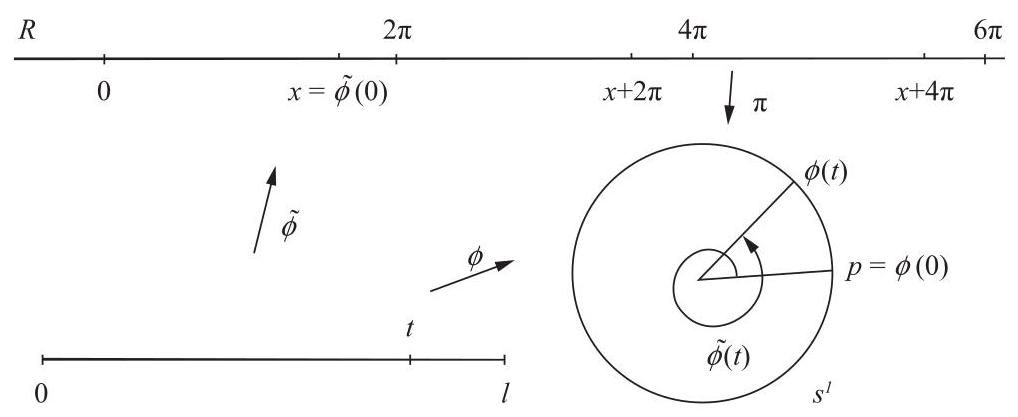
\includegraphics[max width=0.9\textwidth]{images/bo_d4b9jf3ef24c73e0334g_408_274_189_1018_417_0.jpg}
\end{center}
\hspace*{3em} 

图 5-30

设 \({S}^{1} = \left\{  {\left( {x,y}\right)  \in  {R}^{2};{x}^{2} + {y}^{2} = 1}\right\}\) ，并且设 \(\pi  : R \rightarrow  {S}^{1}\) 是由实数线 \(R\) 对 \({S}^{1}\) 的覆盖，由下式给出

\[
\pi \left( x\right)  = \left( {\cos x,\sin x}\right) ,\;x \in  R.
\]

设 \(\varphi  : {S}^{1} \rightarrow  {S}^{1}\) 为一个连续映射. \(\varphi\) 的次数定义如下.我们可以将映射 \(\varphi  : {S}^{1} \rightarrow  {S}^{1}\) 中的第一个 \({S}^{1}\) 看作一个闭区间 \(\left\lbrack  {0,l}\right\rbrack\) ，其端点 0 和 \(l\) 被识别.因此， \(\varphi\) 可以看作一个连续映射 \(\varphi  : \left\lbrack  {0,l}\right\rbrack   \rightarrow  {S}^{1}\) ，其中 \(\varphi \left( 0\right)  = \varphi \left( l\right)  = p \in  {S}^{1}\) .因此， \(\varphi\) 是 \({S}^{1}\) 中 \(p\) 处的闭弧，根据 5-6 节的命题 2，可以提升为一条唯一的弧 \(\widetilde{\varphi } : \left\lbrack  {0,l}\right\rbrack   \rightarrow  R\) ，该弧从 \(x \in  R\) 点开始，具有 \(\pi \left( x\right)  = p\) .由于 \(\pi \left( {\widetilde{\varphi }\left( 0\right) }\right)  = \pi \left( {\widetilde{\varphi }\left( l\right) }\right)\) ，差值 \(\widetilde{\varphi }\left( l\right)  - \widetilde{\varphi }\left( 0\right)\) 是 \({2\pi }\) 的整数倍.整数 \(\deg \varphi\) 由

\[
\widetilde{\varphi }\left( l\right)  - \widetilde{\varphi }\left( 0\right)  = \left( {\deg \varphi }\right) {2\pi }
\]

称为 \(\varphi\) 的次数.

直观地说， \(\deg \varphi\) 是 \(\varphi  : \left\lbrack  {0,l}\right\rbrack   \rightarrow  {S}^{1}\) 将 \(\left\lbrack  {0,l}\right\rbrack\) “缠绕” \({S}^{1}\) 的次数(图 5-30).请注意，函数 \(\widetilde{\varphi } : \left\lbrack  {0,l}\right\rbrack   \rightarrow  R\) 是固定向量 \(\varphi \left( 0\right)  - O\) 与 \(\varphi \left( t\right)  - O,t \in  \lbrack 0,l),O = \left( {0,0}\right)\) 之间的正角的连续确定——例如，5-6 节 A 部分的示例 4 中描述的映射 \(\pi  : {S}^{1} \rightarrow  {S}^{1}\) 的次数为 \(k\) .

我们必须证明次数的定义与 \(p\) 和 \(x\) 的选择无关.

首先，deg \(\varphi\) 与 \(x\) 的选择无关.事实上，设 \({x}_{1} > x\) 为 \(R\) 中的一点，使得 \(\pi \left( {x}_{1}\right)  = p\) ，设 \({\widetilde{\varphi }}_{1}\left( t\right)  = \widetilde{\varphi }\left( t\right)  + \left( {{x}_{1} - x}\right) ,t \in  \left\lbrack  {0,l}\right\rbrack\) .由于 \({x}_{1} - x\) 是 \({2\pi },{\widetilde{\varphi }}_{1}\) 的整数倍， \({2\pi },{\widetilde{\varphi }}_{1}\) 是从 \({x}_{1}\) 开始的 \(\varphi\) 的提升.根据 5-6 节命题 2 的唯一性部分， \({\widetilde{\varphi }}_{1}\) 是从 \({x}_{1}\) 开始的 \(\varphi\) 的提升.由于

\[
{\widetilde{\varphi }}_{1}\left( l\right)  - {\widetilde{\varphi }}_{1}\left( 0\right)  = \widetilde{\varphi }\left( l\right)  - \widetilde{\varphi }\left( 0\right)  = \left( {\deg \varphi }\right) {2\pi },
\]

度 \(\varphi\) 无论用 \(x\) 计算还是用 \({x}_{1}\) 计算都相同.

其次，度 \(\varphi\) 与 \(p \in  {S}^{1}\) 的选择无关.事实上，除了 \(p\) 的对径点外，每个点 \({p}_{1} \in  {S}^{1}\) 都属于 \(p\) 的一个特定邻域 \({U}_{1}\) .选择 \({x}_{1}\) ，在包含 \(x\) 的 \({\pi }^{-1}\left( {U}_{1}\right)\) 的连通分量中，使得 \(\pi \left( {x}_{1}\right)  = {p}_{1}\) ，令 \({\widetilde{\varphi }}_{1}\) 为的提升.

\[
\varphi  : \left\lbrack  {0,l}\right\rbrack   \rightarrow  {S}^{1},\varphi \left( 0\right)  = {p}_{1},
\]

从 \({x}_{1}\) 开始.显然， \(\left| {{\widetilde{\varphi }}_{1}\left( 0\right)  - \widetilde{\varphi }\left( 0\right) }\right|  < {2\pi }\) .通过提升构造的逐步过程(参见命题 2，S-6 节的证明)，可以得出 \(\mid  {\widetilde{\varphi }}_{1}\left( l\right)  - {\widetilde{\varphi }}_{1}\left( l\right)  < {2\pi }\) .由于两个差值 \(\widetilde{\varphi }\left( l\right)  - \widetilde{\varphi }\left( 0\right) ,{\widetilde{\varphi }}_{1}\left( l\right)  - {\widetilde{\varphi }}_{1}\left( 0\right)\) 必须是 \({2\pi }\) 的整数倍，因此它们的值实际上是相等的.根据连续性，该结论也适用于 \(p\) 的对径点，这就证明了我们的主张.

度的最重要的性质是它在同伦下的不变性.更确切地说，设 \({\varphi }_{1},{\varphi }_{2} : {S}^{1} \rightarrow  {S}^{1}\) 为连续映射.固定一个点 \(p \in  {S}^{1}\) ，从而在 \(p,{\varphi }_{1},{\varphi }_{2} : \left\lbrack  {0,l}\right\rbrack   \rightarrow  {S}^{1},{\varphi }_{1}\left( 0\right)  = {\varphi }_{2}\left( 0\right)  = p\) 处得到两条闭合弧.如果 \({\varphi }_{1}\) 和 \({\varphi }_{2}\) 同伦，则 \(\deg {\varphi }_{1} = \deg {\varphi }_{2}\) .这直接源于(命题 4，5-6 节)从固定点 \(x \in  R\) 开始的 \({\varphi }_{1}\) 和 \({\varphi }_{2}\) 的提升是同伦的，因此具有相同的终点.

应该指出的是，如果 \(\varphi  : \left\lbrack  {0,l}\right\rbrack   \rightarrow  {S}^{1}\) 是可微的，它就确定了可微函数 \(a = a\left( t\right) ,b = b\left( t\right)\) ，由 \(\varphi \left( t\right)  = \left( {a\left( t\right) ,b\left( t\right) }\right)\) 给出，它们满足条件 \({a}^{2} + {b}^{2} = 1\) .在这种情况下，从 \({\widetilde{\varphi }}_{0} = x\) 开始的提升 \(\widetilde{\varphi }\) 正是可微函数(参见引理 1，4-4 节).

\[
\widetilde{\varphi }\left( t\right)  = {\widetilde{\varphi }}_{0} + {\int }_{0}^{t}\left( {a{b}^{\prime } - b{a}^{\prime }}\right) {dt}.
\]

这源于提升的唯一性和 \(\cos \widetilde{\varphi }\left( t\right)  = a\left( t\right)\) , \(\sin \widetilde{\varphi }\left( t\right)  = b\left( t\right) ,\widetilde{\varphi }\left( 0\right)  = {\widetilde{\varphi }}_{0}\) 的事实.因此，在可微情况下， \(\varphi\) 的次数可以用积分表示，

\[
\deg \varphi  = \frac{1}{2\pi }{\int }_{0}^{l}\frac{d\widetilde{\varphi }}{dt}{dt}.
\]

在后一种形式中，次数的概念在本书中反复出现.例如，当 \(v : U \subset  {R}^{2} \rightarrow  {R}^{2},U \supset  {S}^{1}\) 是一个向量场，而 \(\left( {0,0}\right)\) 是其唯一的奇点时， \(v\) 在 \(\left( {0,0}\right)\) 处的指数(参见第 4-5 节，应用 7)可以解释为映射 \(\varphi  : {S}^{1} \rightarrow  {S}^{1}\) 的次数，该映射由 \(\varphi \left( p\right)  = v\left( p\right) /\left| {v\left( p\right) }\right| ,p \in  {S}^{1}.\) 给出

在给出更多例子之前，让我们回顾一下，一个闭合的(可微)曲线是一个可微映射 \(\alpha  : \left\lbrack  {0,l}\right\rbrack   \rightarrow  {R}^{3}\) (如果是平面曲线，则为 \({R}^{2}\) )，使得 \(\alpha\) 的分量及其所有导数在 0 和 \(l\) 处一致.曲线 \(\alpha\) 是正则的，如果对于所有 \(t \in  \left\lbrack  {0,l}\right\rbrack\) 都有 \({\alpha }^{\prime }\left( t\right)  \neq  0\) ，并且 \(\alpha\) 是简单的，如果当 \({t}_{1} \neq  {t}_{2},{t}_{1},{t}_{2} \in  \lbrack 0,l)\) 时，则 \(\alpha \left( {t}_{1}\right)  \neq  \alpha \left( {t}_{2}\right)\) .有时我们假设 \(\alpha\) 仅仅是连续的；在这种情况下，我们将明确说明 \(\alpha\) 是一个连续的闭合曲线.

示例 1(曲线的绕数).设 \(\alpha  : \left\lbrack  {0,l}\right\rbrack   \rightarrow  {R}^{2}\) 为一个平面连续闭合曲线.选择一个点 \({p}_{0} \in  {R}^{2},{p}_{0} \notin  \alpha \left( \left\lbrack  {0,l}\right\rbrack  \right)\) ，令 \(\varphi  : \left\lbrack  {0,l}\right\rbrack   \rightarrow  {S}^{1}\) 由下式给出

\[
\varphi \left( t\right)  = \frac{\alpha \left( t\right)  - {P}_{0}}{\left| \alpha \left( t\right)  - {P}_{0}\right| },\;t \in  \left\lbrack  {0,l}\right\rbrack  .
\]

显然 \(\varphi \left( 0\right)  = \varphi \left( l\right)\) ，并且 \(\varphi\) 可以被认为是 \({S}^{1}\) 到 \({S}^{1}\) 的映射；它被称为 \(\alpha\) 相对于 \({p}_{0}\) 的位置映射. \(\varphi\) 的次数被称为曲线 \(\alpha\) 相对于 \({p}_{0}\) 的绕数(或指数)(图 5-31).

\begin{center}
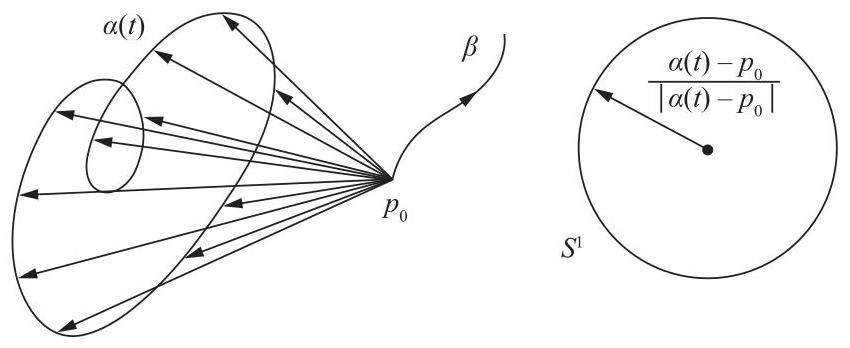
\includegraphics[max width=0.7\textwidth]{images/bo_d4b9jf3ef24c73e0334g_410_362_793_850_348_0.jpg}
\end{center}
\hspace*{3em} 

图 5-31

注意到，当 \({p}_{0}\) 沿着一条不与 \(\alpha \left( \left\lbrack  {0,l}\right\rbrack  \right)\) 相交的弧 \(\beta\) 移动时，绕数保持不变.事实上， \(\alpha\) 相对于 \(\beta\) 的任意两点的位移映射可以清楚地由一个同伦连接.因此，当 \(q\) 在 \({R}^{2} - \alpha \left( \left\lbrack  {0,l}\right\rbrack  \right)\) 的一个连通分量中运行时， \(\alpha\) 相对于 \(q\) 的绕数是常数.

例 2(曲线的旋转指数).设 \(\alpha  : \left\lbrack  {0,l}\right\rbrack   \rightarrow  {R}^{2}\) 为一条正则平面闭合曲线，令 \(\varphi  : \left\lbrack  {0,l}\right\rbrack   \rightarrow  {S}^{1}\) 由下式给出:

\[
\varphi \left( t\right)  = \frac{{\alpha }^{\prime }\left( t\right) }{\left| {\alpha }^{\prime }\left( t\right) \right| },\;t \in  \left\lbrack  {0,l}\right\rbrack
\]

显然 \(\varphi\) 是可微的， \(\varphi \left( 0\right)  = \varphi \left( l\right) .\varphi\) 称为 \(\alpha\) 的切映射， \(\varphi\) 的次数称为 \(\alpha\) 的旋转指数.直观地说，闭合曲线的旋转指数是沿着曲线的切向量场给出的完整转弯次数(图 1-27，节 1-7).

通过使用顶点处的角度(见节 4-5)，可以将旋转指数的概念推广到分段正则曲线，并证明简单、闭合、分段正则曲线的旋转指数是 \(\pm  1\) (转切定理).这一事实用于高斯-博内定理的证明.在本节后面，我们将证明转切定理的可微版本.

我们的第一个全局定理将是所谓的约当曲线定理的可微版本.为了证明，我们将假定对节 2-7 的材料有所了解.

定理 1(可微约当曲线定理).设 \(\alpha  : \left\lbrack  {0,l}\right\rbrack \; \rightarrow  {\mathbb{R}}^{2}\) 为一条平面、正则、闭合、简单曲线.则 \({\mathbb{R}}^{2} \rightarrow  \alpha \left( \left\lbrack  {0,l}\right\rbrack  \right)\) 有且仅有两个连通分量，而 \(\alpha \left( \left\lbrack  {0,l}\right\rbrack  \right) )\) 是它们的公共边界.

证明. 令 \({N}_{\epsilon }\left( \alpha \right)\) 为 \(\alpha \left( \left\lbrack  {0,l}\right\rbrack  \right)\) 的一个管状邻域. 其构造方式与紧致曲面的管状邻域的构造方式相同 (参见第 2-7 节). 我们回顾 \({N}_{\epsilon }\left( \alpha \right)\) 是具有长度 \({2\epsilon }\) 且中心位于 \(\alpha \left( t\right)\) 的开法线段 \({I}_{\epsilon }\left( t\right)\) 的并集. 显然, \({N}_{\epsilon }\left( \alpha \right)  - \alpha \left( \left\lbrack  {0,l}\right\rbrack  \right)\) 有两个连通分量 \({T}_{1}\) 和 \({T}_{2}\) . 令 \(w\left( p\right)\) 为 \(\alpha\) 相对于 \(p \in  {R}^{2} - \alpha \left( \left\lbrack  {0,l}\right\rbrack  \right)\) 的绕数. 证明的关键在于表明, 如果 \({p}_{1}\) 和 \({p}_{2}\) 都属于 \({N}_{\epsilon }\left( \alpha \right)  - \alpha \left( \left\lbrack  {0,l}\right\rbrack  \right)\) 的不同连通分量, 并且属于同一个 \({I}_{\epsilon }\left( {t}_{0}\right) ,{t}_{0} \in  \left\lbrack  {0,l}\right\rbrack\) , 那么 \(w\left( {p}_{1}\right)  - w\left( {p}_{2}\right)  =  \pm  1\) , 其符号取决于 \(\alpha\) 的方向.

选择点 \(A = \alpha \left( {t}_{1}\right) ,D = \alpha \left( {t}_{2}\right) ,{t}_{1} < {t}_{0} < {t}_{2}\) , 使其足够靠近 \({t}_{0}\) , 以至于 \(\alpha\) 的弧 \({AD}\) 可以通过同伦变形到图 5-32 的多边形 \({ABCD}\) . 这里 \({BC}\) 是切线在 \(\alpha \left( t\right)\) 处的线段, 而 \({BA}\) 和 \({CD}\) 平行于法线在 \(\alpha \left( {t}_{0}\right)\) 处.

令 \(\beta  : \left\lbrack  {0,\bar{l}}\right\rbrack   \rightarrow  {R}^{2}\) 表示通过将弧 \({AD}\) 替换为多边形 \({ABCD}\) 从 \(\alpha\) 得到的曲线, 并假设 \(\beta \left( 0\right)  = \beta \left( \bar{l}\right)  = A\) 且 \(\beta \left( {t}_{3}\right)  = D\) . 显然, \(w\left( {p}_{1}\right)\) 和 \(w\left( {p}_{2}\right)\) 保持不变.

令 \({\varphi }_{1},{\varphi }_{2} : \left\lbrack  {0,\bar{l}}\right\rbrack   \rightarrow  {S}^{1}\) 分别为 \(\beta\) 相对于 \({p}_{1},{p}_{2}\) 的位置映射 (参见示例 1), 并令 \({\widetilde{\varphi }}_{1},{\widetilde{\varphi }}_{2} : \left\lbrack  {0,\bar{l}}\right\rbrack   \rightarrow  R\) 为从固定点 (例如 \(0 \in  R\) ) 的提升. 为方便起见, 假设 \(\beta\) 的方向如图 5-32 所示.

我们首先注意到，如果 \(t \in  \left\lbrack  {{t}_{3},\bar{l}}\right\rbrack\) ，则 \(\alpha \left( t\right)\) 到 \({p}_{1}\) 和 \({p}_{2}\) 的距离有下界，该下界独立于 \(t\) ，即 \(\operatorname{dist}\left( {{p}_{1},\operatorname{Bd}{N}_{\epsilon }\left( \alpha \right) }\right)\) 和 \(\operatorname{dist}\left( {{p}_{2},\operatorname{Bd}{N}_{\epsilon }\left( \alpha \right) }\right)\) 中较小者.因此， \(\alpha \left( t\right)  - {p}_{1}\) 与 \(\alpha \left( t\right)  - {p}_{2}\) 的夹角在 \(\left( {{t}_{3},\bar{l}}\right\rbrack\) 中随着 \({p}_{1}\) 趋近于 \({p}_{2}\) 而均匀趋近于零.

现在，显然可以选择 \({p}_{1}\) 和 \({p}_{2}\) 彼此非常接近，以至于 \({\widetilde{\varphi }}_{1}\left( {t}_{3}\right)  - {\widetilde{\varphi }}_{1}\left( 0\right)  = \pi  - {\epsilon }_{1}\) 和 \({\widetilde{\varphi }}_{2}\left( {t}_{3}\right)  - {\widetilde{\varphi }}_{2}\left( 0\right)  =  - \left( {\pi  + {\epsilon }_{2}}\right)\) ，其中 \({\epsilon }_{1}\) 和 \({\epsilon }_{2}\) 小于 \(\pi /3\) .此外，

\[
{2\pi }\left( {w\left( {p}_{1}\right)  - w\left( {p}_{2}\right) }\right)  = \left( {{\widetilde{\varphi }}_{1}\left( \bar{l}\right)  - {\widetilde{\varphi }}_{1}\left( 0\right)  - \left( {{\widetilde{\varphi }}_{2}\left( \bar{l}\right)  - {\widetilde{\varphi }}_{2}\left( 0\right) }\right) }\right.
\]

\[
= \left\{  {\left( {{\widetilde{\varphi }}_{1} - {\widetilde{\varphi }}_{2}}\right) \left( \widetilde{l}\right)  - \left( {{\widetilde{\varphi }}_{1} - {\widetilde{\varphi }}_{2}}\right) \left( {t}_{3}\right) }\right\}
\]

\[
+ \left\{  {\left( {{\widetilde{\varphi }}_{1} - {\widetilde{\varphi }}_{2}}\right) \left( {t}_{3}\right)  - \left( {{\widetilde{\varphi }}_{1} - {\widetilde{\varphi }}_{2}}\right) \left( 0\right) }\right\}  .
\]

\begin{center}
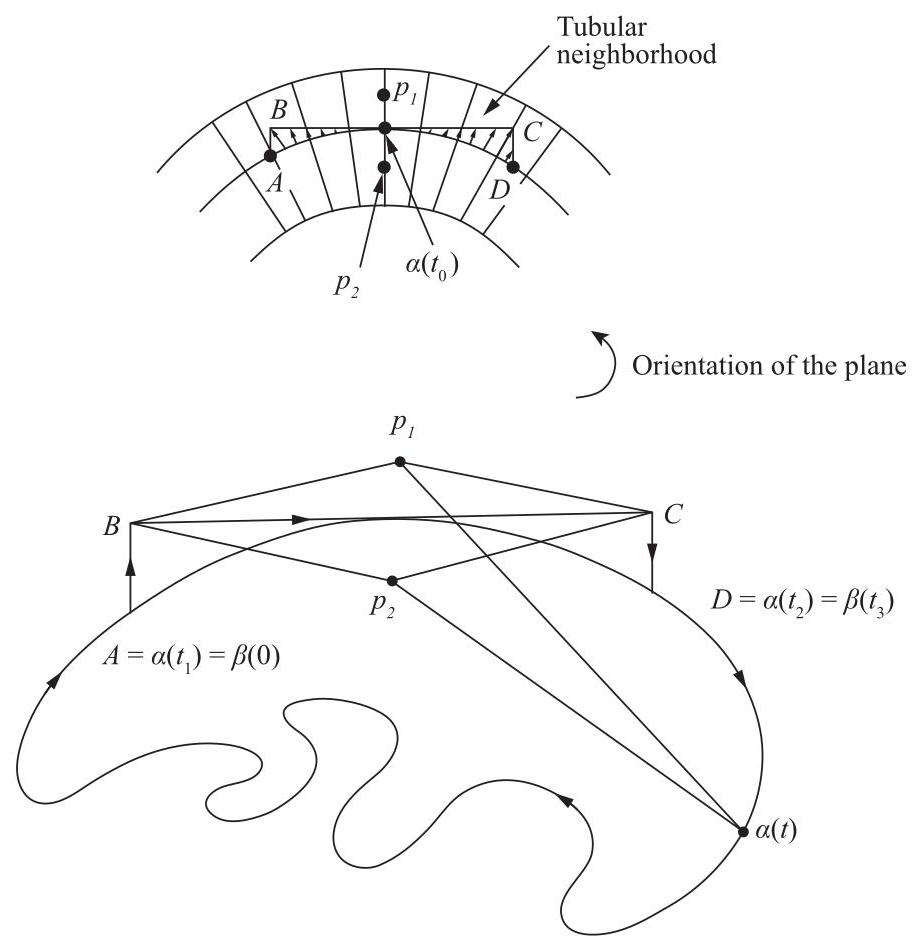
\includegraphics[max width=0.8\textwidth]{images/bo_d4b9jf3ef24c73e0334g_412_326_192_921_945_0.jpg}
\end{center}
\hspace*{3em} 

图 5-32

根据上述评论，第一项可以任意小，例如等于 \({\epsilon }_{1} < \pi /3\) ，如果 \({p}_{1}\) 足够接近 \({p}_{2}\) .因此，

\[
{2\pi }\left( {w\left( {p}_{1}\right)  - w\left( {p}_{2}\right) }\right)  = {\epsilon }_{3} + \pi  - {\epsilon }_{1} - \left( {-\pi  - {\epsilon }_{2}}\right)  = {2\pi } + \epsilon ,
\]

其中 \(\epsilon  < \pi\) ，如果 \({p}_{1}\) 足够接近 \({p}_{2}\) .因此， \(w\left( {p}_{1}\right)  - w\left( {p}_{2}\right)  = 1\) ，正如我们所声称的.

现在很容易完成证明.由于 \(w\left( p\right)\) 在 \({R}^{2} - \alpha \left( \left\lbrack  {0,l}\right\rbrack  \right)  = W\) 的每个连通分量中是常数，因此从上面可以得出 \(W\) 中至少有两个连通分量.我们将证明恰好有两个这样的分量.

事实上，令 \(C\) 为 \(W\) 的一个连通分量.显然有 Bd \(C \neq  \phi\) 和 Bd \(C \subset  \alpha \left( \left\lbrack  {0,l}\right\rbrack  \right)\) .另一方面，如果 \(p \in  \alpha \left( \left\lbrack  {0,l}\right\rbrack  \right)\) ，则存在 \(p\) 的一个邻域，该邻域仅包含 \(\alpha \left( \left\lbrack  {0,l}\right\rbrack  \right)\) 的点、 \({T}_{1}\) 的点，以及 \({T}_{2}\left( {T}_{1}\right.\) 和 \({T}_{2}\) 是 \({N}_{\epsilon }\left( \alpha \right)  - \alpha \left( \left\lbrack  {0,l}\right\rbrack  \right) )\) 的连通分量.因此， \({T}_{1}\) 或 \({T}_{2}\) 与 \(C\) 相交.由于 \(C\) 是一个连通分量， \(C \supset  {T}_{1}\) 或 \(C \supset  {T}_{2}\) .因此， \(W\) 最多有两个(因此，恰好有两个)连通分量.将它们表示为 \({C}_{1}\) 和 \({C}_{2}\) .该论证也表明 \(\operatorname{Bd}{C}_{1} = \; \alpha \left( \left\lbrack  {O,l}\right\rbrack  \right)  = \operatorname{Bd}{C}_{2}.\)Q.E.D.

定理 1 给出的两个连通分量很容易区分.一个基于这样的观察:如果 \({p}_{0}\) 位于包含 \(\alpha \left( \left\lbrack  {0,l}\right\rbrack  \right)\) 的闭圆盘 \(D\) 的外部(因为 \(\left\lbrack  {0,l}\right\rbrack\) 是紧致的，所以这样的圆盘存在)，那么相对于 \({p}_{0}\) 的 \(\alpha\) 的绕数是零.这是因为连接 \({p}_{0}\) 和 \(\alpha \left( t\right) ,t \in  \left\lbrack  {0,l}\right\rbrack\) 的直线都位于一个包含 \(D\) 且由从 \({p}_{0}\) 到圆周 Bd \(D\) 的两条切线所界定的区域内.因此，绕数为零的连通分量是无界的，并且包含所有在某个圆盘外部的点.显然，剩余的连通分量具有绕数 \(\pm  1\) 并且是有界的.通常将它们分别称为 \(\alpha\) 的外部和内部.

注 1. 上述定理的一个有用的补充，它在 Gauss-Bonnet 定理的应用(第 4-5 节)中使用过，是 \(\alpha\) 的内部同胚于一个开圆盘.可以在 J. J. Stoker 的《微分几何》(Wiley-Interscience，纽约，1969 年，第 43-45 页)中找到证明.

现在我们将证明一个可微版本的转切线定理.

定理 2. 令 \(\beta  : \left\lbrack  {0,l}\right\rbrack   \rightarrow  {\mathbb{R}}^{2}\) 为一个平面上的正则、简单、闭合曲线.则 \(\beta\) 的旋转指数为 \(\pm  1\) (取决于 \(\beta\) 的方向).

证明.考虑一条不与曲线相交的直线，并将其平行移动，直到它与曲线相切.令 \(L\) 表示该直线的位置，令 \(p\) 表示曲线与 \(L\) 的切点.显然，曲线完全位于 \(L\) 的一侧(图 5-33).为曲线选择一个新的参数化 \(\alpha  : \left\lbrack  {0,l}\right\rbrack   \rightarrow  {R}^{2}\) ，使得 \(\alpha \left( 0\right)  = p\) .现在令

\[
T = \left\{  {\left( {{t}_{1},{t}_{2}}\right)  \in  \left\lbrack  {0,l}\right\rbrack   \times  \left\lbrack  {0,l}\right\rbrack  ;0 \leq  {t}_{1} \leq  {t}_{2} \leq  l}\right\}
\]

定义一个“割线映射” \(\psi  : T \rightarrow  {S}^{1}\) ，使其为一个三角形，并

\[
\psi \left( {{t}_{1},{t}_{2}}\right)  = \frac{\alpha \left( {t}_{2}\right)  - \alpha \left( {t}_{1}\right) }{\left| \alpha \left( {t}_{2}\right)  - \alpha \left( {t}_{1}\right) \right| }\;\text{ for }{t}_{1} \neq  {t}_{2},\left( {{t}_{1},{t}_{2}}\right)  \in  T - \{ \left( {0,l}\right) \}
\]

\[
\psi \left( {t,t}\right)  = \frac{{\alpha }^{\prime }\left( t\right) }{\left| {\alpha }^{\prime }\left( {t}_{2}\right) \right| },\;\psi \left( {0,l}\right)  =  - \frac{{\alpha }^{\prime }\left( 0\right) }{\left| {\alpha }^{\prime }\left( 0\right) \right| }.
\]

由于 \(\alpha\) 是正则的， \(\psi\) 很容易被看作是连续的.设 \(A = \left( {0,0}\right) ,B = \; \left( {0,l}\right) ,C = \left( {l,l}\right)\) 为三角形 \(T\) 的顶点.注意到 \(\psi\) 在边 \({AC}\) 上的限制是 \(\alpha\) 的切线映射，其次数是 \(\alpha\) 的旋转数.显然(图 5-33)，切线映射与 \(\psi\) 在剩余边 \({AB}\) 和 \({BC}\) 上的限制是同伦的.因此，我们只需证明后者的次数是 \(\pm  1\) .

假设平面和曲线的方向使得从 \({\alpha }^{\prime }\left( 0\right)\) 到 \(- {\alpha }^{\prime }\left( 0\right)\) 的定向角为 \(\pi\) .那么 \(\psi\) 在 \({AB}\) 上的限制以正方向覆盖了 \({S}^{1}\) 的一半，而 \(\psi\) 在 \({BC}\) 上的限制也以正方向覆盖了剩余的一半(图 5-33).因此， \(\psi\) 在 \({AB}\) 和 \({BC}\) 上的限制的次数为 +1.反转方向，我们将得到 -1 的次数，这就完成了证明.Q.E.D.

\begin{center}
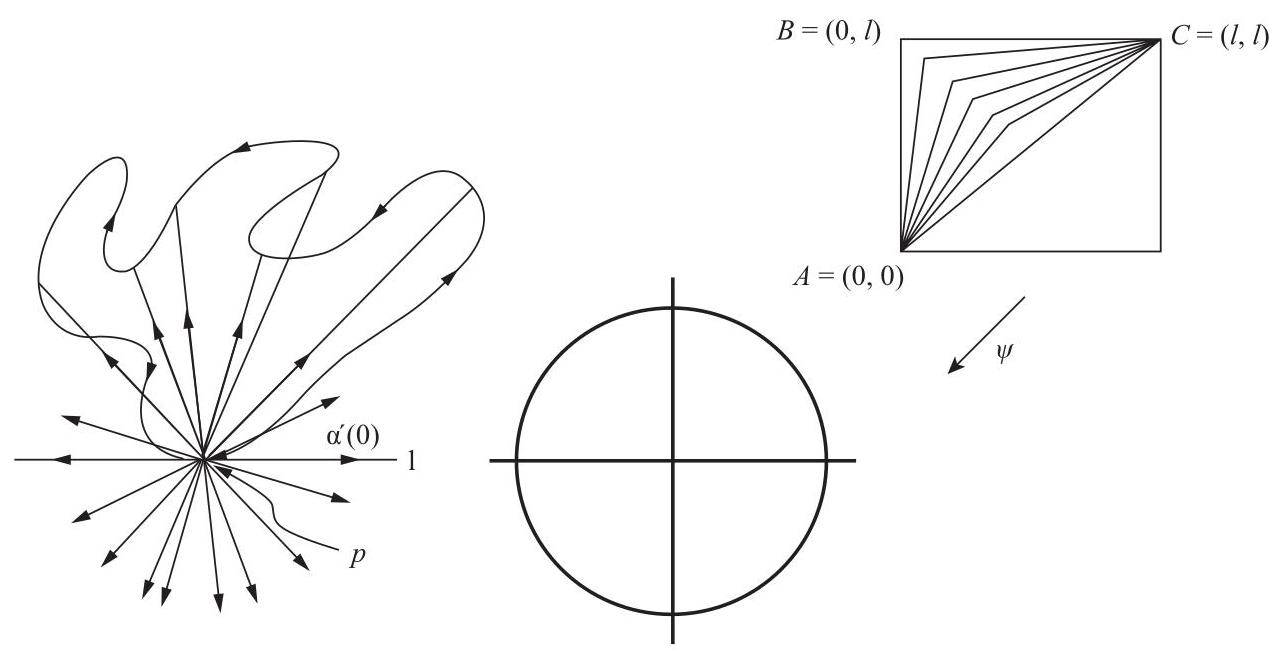
\includegraphics[max width=1.0\textwidth]{images/bo_d4b9jf3ef24c73e0334g_414_171_191_1283_654_0.jpg}
\end{center}
\hspace*{3em} 

图 5-33

切线定理可用于表征一类重要的曲线，即凸曲线.

平面上的正则闭合曲线 \(\alpha  : \left\lbrack  {0,l}\right\rbrack   \rightarrow  {R}^{2}\) 是凸的，如果对于每个 \(t \in \; \left\lbrack  {0,l}\right\rbrack\) ，曲线位于由 \(t\) 处的切线确定的一个闭合半平面内(图 5-34；参见第 1-7 节).如果 \(\alpha\) 是单的，凸性可以用曲率来表示.我们回顾一下，对于平面曲线，曲率始终表示有向曲率(第 1-5 节，注 1).

\begin{center}
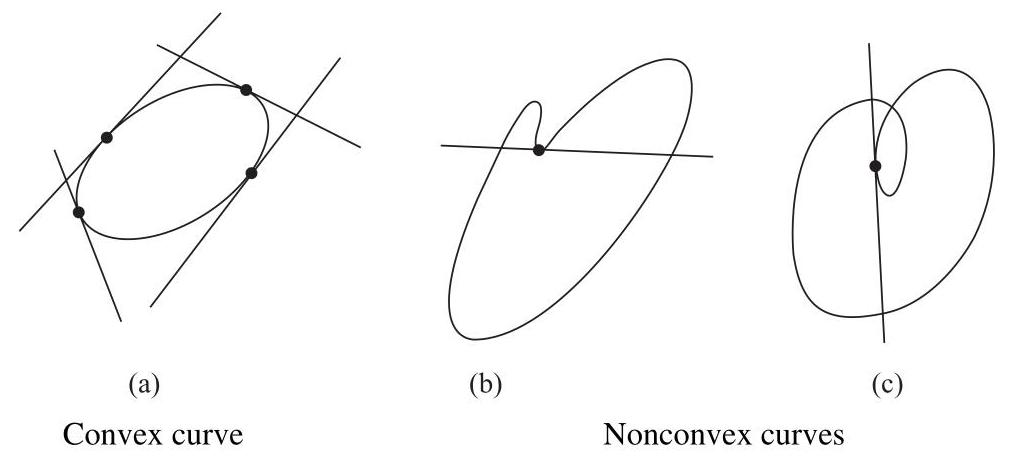
\includegraphics[max width=0.9\textwidth]{images/bo_d4b9jf3ef24c73e0334g_414_253_1589_1011_458_0.jpg}
\end{center}
\hspace*{3em} 

图 5-34

命题 1. 平面上的正则闭合曲线是凸的，当且仅当它是单的且其曲率 \(\mathrm{k}\) 不改变符号.

证明.设 \(\varphi  : \left\lbrack  {0,l}\right\rbrack   \rightarrow  {S}^{1}\) 为 \(\alpha\) 的切线映射， \(\widetilde{\varphi } : \left\lbrack  {0,l}\right\rbrack   \rightarrow  R\) 为从 \(0 \in  R\) 开始的 \(\varphi\) 的提升.我们首先注意到 \(k\) 不改变符号的条件等价于 \(\widetilde{\varphi }\) 是单调的(如果 \(k \geq  0\) 则非递减，如果 \(k \leq  0\) 则非递增).

现在，假设 \(\alpha\) 是单的且 \(k\) 不改变符号.我们可以定向曲线所在的平面，使得 \(k \geq  0\) .假设 \(\alpha\) 不是凸的.那么存在 \({t}_{0} \in  \left\lbrack  {0,l}\right\rbrack\) ，使得 \(\alpha \left( \left\lbrack  {0,l}\right\rbrack  \right)\) 的点可以在 \(\alpha \left( {t}_{0}\right)\) 处的切线 \(T\) 的两侧找到.设 \(n = n\left( {t}_{0}\right)\) 为 \({t}_{0}\) 处的法向量，并令

\[
{h}_{n}\left( t\right)  = \left\langle  {\alpha \left( t\right)  - \alpha \left( {t}_{0}\right) ,n}\right\rangle  ,\;t \in  \left\lbrack  {0,l}\right\rbrack  .
\]

由于 \(\left\lbrack  {0,l}\right\rbrack\) 是紧致的，并且 \(T\) 的两侧都包含曲线上的点，因此“高度函数” \({h}_{n}\) 在 \({t}_{1} \neq  {t}_{0}\) 处取得最大值，在 \({t}_{2} \neq  {t}_{0}\) 处取得最小值.点 \({t}_{0},{t}_{1},{t}_{2}\) 处的切向量都平行，因此其中两个，例如 \({\alpha }^{\prime }\left( {t}_{0}\right) ,{\alpha }^{\prime }\left( {t}_{1}\right)\) ，具有相同的方向.由此得出 \(\varphi \left( {t}_{0}\right)  = \varphi \left( {t}_{1}\right)\) ，并且根据定理 2( \(\alpha\) 是单叶的)，得出 \(\widetilde{\varphi }\left( {t}_{0}\right)  = \widetilde{\varphi }\left( {t}_{1}\right)\) .我们假设 \({t}_{1} > {t}_{0}\) .根据上述评论， \(\widetilde{\varphi }\) 是单调非递减的，因此在 \(\left\lbrack  {{t}_{0},{t}_{1}}\right\rbrack\) 中是常数.这意味着 \(\alpha \left( \left\lbrack  {{t}_{0},{t}_{1}}\right\rbrack  \right)  \subset  T\) .但这与 \(T\) 的选择相矛盾，并表明 \(\alpha\) 是凸的.

反之，假设 \(\alpha\) 是凸的.我们将把它留作练习，以证明如果 \(\alpha\) 不是单叶的，在自交点(图 5-35(a))或其附近(图 5-35(b))，凸性条件被违反.因此， \(\alpha\) 是单叶的.

\begin{center}
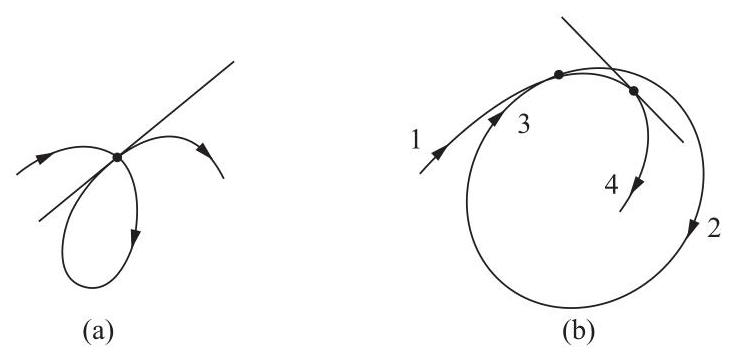
\includegraphics[max width=0.6\textwidth]{images/bo_d4b9jf3ef24c73e0334g_415_398_1285_731_357_0.jpg}
\end{center}
\hspace*{3em} 

图 5-35

我们现在假设 \(\alpha\) 是凸的，并且 \(k\) 在 \(\left\lbrack  {0,l}\right\rbrack\) 中改变符号.那么存在点 \({t}_{1},{t}_{2} \in  \left\lbrack  {0,l}\right\rbrack  ,{t}_{1} < {t}_{2}\) ，其中 \(\widetilde{\varphi }\left( {t}_{1}\right)  = \widetilde{\varphi }\left( {t}_{2}\right)\) 且 \(\left\lbrack  {{t}_{1},{t}_{2}}\right\rbrack\) 中的 \(\widetilde{\varphi }\) 不是常数.

我们将证明这会导致矛盾，从而完成证明.根据定理 2，存在 \({t}_{3} \in  \lbrack 0,l)\) 使得 \(\varphi \left( {t}_{3}\right)  =  - \varphi \left( {t}_{1}\right)\) .根据凸性， \(\alpha \left( {t}_{1}\right) ,\alpha \left( {t}_{2}\right) ,\alpha \left( {t}_{3}\right)\) 处的三个平行切线中的两条必须重合.假设 \(\alpha \left( {t}_{1}\right)  = p,\alpha \left( {t}_{3}\right)  = q,{t}_{3} > {t}_{1}\) 的情况如此.我们声称 \(\alpha\) 在 \(p\) 和 \(q\) 之间的弧是线段 \({pq}\) .

事实上，假设 \(r \neq  q\) 是最后一个使得该弧是线段 \(\left( {r\text{ may agree with }p}\right)\) 的点.由于曲线位于直线 \({pq}\) 的同一侧，很容易看出 \(p\) 附近的某个切线 \(T\) 将在内点处穿过线段 \(\overline{pq}\) (图 5-36).那么 \(p\) 和 \(q\) 位于 \(T\) 的两侧.这是一个矛盾，证明了我们的主张.

\begin{center}
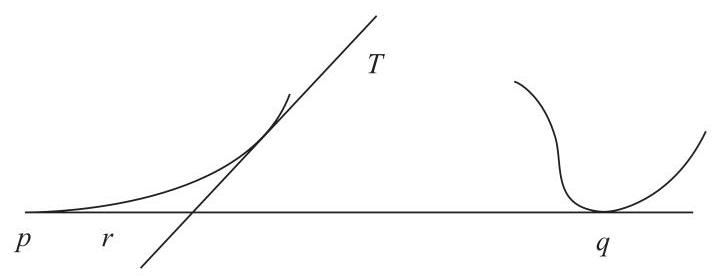
\includegraphics[max width=0.6\textwidth]{images/bo_d4b9jf3ef24c73e0334g_416_424_452_719_279_0.jpg}
\end{center}
\hspace*{3em} 

图 5-36

由此可知，重合的切线具有相同的方向；也就是说，它们实际上是 \(\alpha \left( {t}_{1}\right)\) 和 \(\alpha \left( {t}_{2}\right)\) 处的切线.因此， \(\widetilde{\varphi }\) 在 \(\left\lbrack  {{t}_{1},{t}_{2}}\right\rbrack\) 中是常数，这个矛盾证明了 \(k\) 在 \(\left\lbrack  {0,l}\right\rbrack\) 中不改变符号.

Q.E.D.

注2. 如图5-34(c)所示的曲线的例子表明， \(\alpha\) 是简单的这个条件对该命题是必不可少的.

注3. 该命题应与第5-6节的注2和注3进行比较；那里指出，曲面也存在类似的情况.值得注意的是，在曲面的情况下，不存在自交点不是一个假设，而是一个推论.

注4. 可以证明，一个平面、正则、闭合的曲线是凸的，当且仅当它的内部是一个凸集 \(K \subset  {R}^{2}\) (参见练习4).

我们现在将注意力转向空间曲线.在下文中，曲线一词将表示以弧长 \(s\) 为参数的参数化正则曲线 \(\alpha  : \left\lbrack  {0,l}\right\rbrack   \rightarrow  {R}^{3}\) .如果 \(\alpha\) 是平面曲线，则曲率 \(k\left( s\right)\) 是 \(\alpha\) 的有符号曲率 (参见第1-5节)；否则，假定 \(k\left( s\right)\) 对所有 \(s \in  \left\lbrack  {0,l}\right\rbrack\) 都为正.方便地称

\[
{\int }_{0}^{l}\left| {k\left( s\right) }\right| {ds}
\]

为 \(\alpha\) 的总曲率.

关于空间曲线最著名的全局定理可能是所谓的 Fencbel 定理.

定理3 (Feochel 定理).简单闭合曲线的总曲率是 \(\geq  {2\pi }\) ，当且仅当该曲线是平面凸曲线时，等式成立.

在进行证明之前，我们将介绍一个辅助曲面，它对于定理4的证明也很有用.

曲线 \(\alpha\) 周围半径为 \(r\) 的管是参数化曲面

\[
\mathbf{x}\left( {s,v}\right)  = \alpha \left( s\right)  + r\left( {n\cos v + b\sin v}\right) ,\;s \in  \left\lbrack  {0,l}\right\rbrack  ,v \in  \left\lbrack  {0,{2\pi }}\right\rbrack  ,
\]

其中 \(n = n\left( s\right)\) 和 \(b = b\left( s\right)\) 分别是 \(\alpha\) 的法向量和副法向量.很容易检查出

\[
{\left| {\mathbf{x}}_{s} \land  {\mathbf{x}}_{v}\right| }^{2} = {EG} - {F}^{2} = {r}^{2}{\left( 1 - rk\cos v\right) }^{2}.
\]

我们假设 \(r\) 非常小，以至于 \(r{k}_{0} < I\) ，其中 \({k}_{0} < \max \left| {k\left( s\right) }\right| ,s \in  \left\lbrack  {0,l}\right\rbrack\) .那么 \(\mathbf{x}\) 是正则的，直接计算得到

\[
N =  - \left( {n\cos v + b\sin v}\right) ,
\]

\[
{\mathbf{x}}_{s} \land  {\mathbf{x}}_{v} = r\left( {1 - {rk}\cos v}\right) N
\]

\[
{N}_{s} \land  {N}_{v} = k\cos v\left( {n\cos v + b\sin v}\right)  =  - {kN}\cos v
\]

\[
=  - \frac{k\cos v}{r\left( {1 - {rk}\cos v}\right) }{\mathbf{x}}_{v} \land  {\mathbf{x}}_{s}.
\]

由此可知，管的 \(K = K\left( {s,v}\right)\) 高斯曲率由下式给出

\[
K\left( {s,v}\right)  =  - \frac{k\cos v}{r\left( {1 - {rk}\cos v}\right) }.
\]

请注意， \(\mathbf{x}\) 的迹 \(T\) 可能有自交点.然而，如果 \(\alpha\) 是简单的，可以选择 \(r\) 足够小以避免这种情况；我们利用 \(\left\lbrack  {0,l}\right\rbrack\) 的紧致性，并按照第2-7节中构造的管状邻域的情况进行.如果此外 \(\alpha\) 是闭合的，则 \(T\) 是一个正则曲面，同胚于一个环面，也称为 \(\alpha\) 周围的管.在下文中，我们假定是这种情况.

定理3的证明.设 \(T\) 是 \(\alpha\) 周围的一个管，设 \(R \subset  T\) 是 \(T\) 中高斯曲率为非负的区域.一方面，

\[
{\iint }_{R}{Kd\sigma } = {\iint }_{R}K\sqrt{{EG} - {F}^{2}}{dsdv}
\]

\[
= {\int }_{0}^{l}{kds}{\int }_{\pi /2}^{{3\pi }/2}\cos {vdv} = 2{\int }_{0}^{l}k\left( s\right) {ds}.
\]

另一方面，每条穿过 \({R}^{3}\) 原点的半直线 \(L\) 至少出现一次作为 \(R\) 的法线方向.因为如果我们取一个垂直于 \(L\) 的平面 \(P\) ，使得 \(P \cap  T = \phi\) ，并将 \(P\) 沿自身方向平行移动趋近 \(T\) (图 5-37)，它将第一次遇到 \(T\) ，此时 \(K \geq  0\) .

\begin{center}
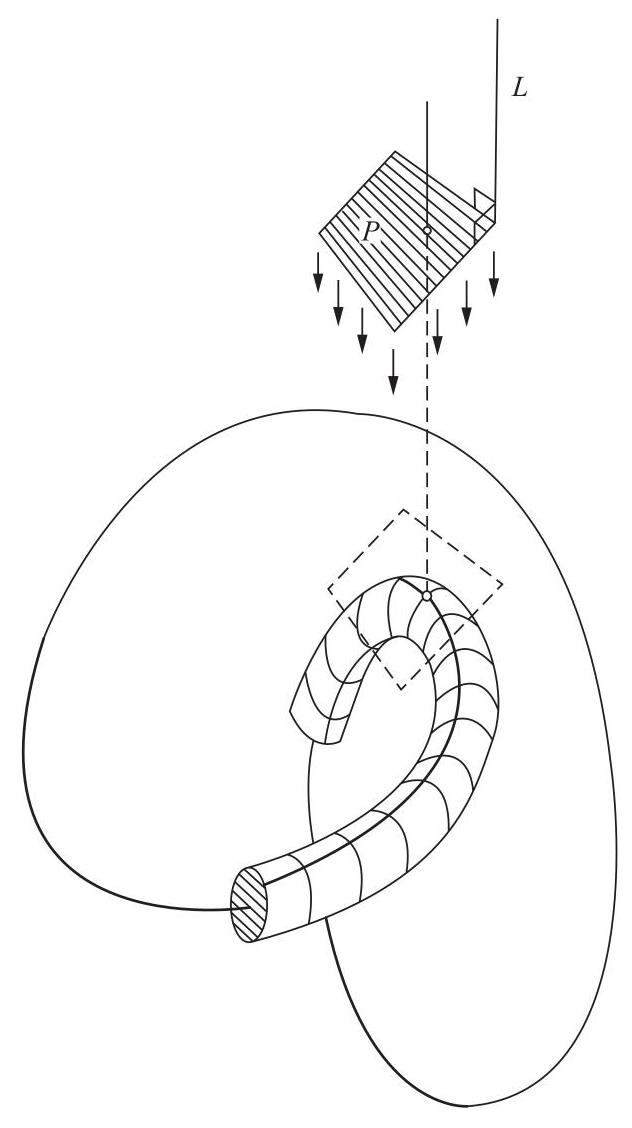
\includegraphics[max width=0.5\textwidth]{images/bo_d4b9jf3ef24c73e0334g_418_187_186_632_1128_0.jpg}
\end{center}
\hspace*{3em} 

图 5-37

由此可知， \(R\) 的高斯映射 \(N\) 至少覆盖整个单位球面 \({S}^{2}\) 一次；因此， \({\iint }_{R}{Kd\sigma } \geq  {4\pi }\) .所以， \(\alpha\) 的总曲率为 \(\geq  {2\pi }\) ，我们证明了定理 3 的第一部分.

观察到高斯映射 \(N\) 在每个常数圆 \(s =\) 上的像是一一对应的，并且其像是一个大圆 \({\Gamma }_{s} \subset  {S}^{2}\) .我们将用 \({\Gamma }_{s}^{ + } \subset  {\Gamma }_{s}\) 来表示对应于 \(K \geq  0\) 的点的闭合半圆.

假设 \(\alpha\) 是一个平面凸曲线.那么所有 \({\Gamma }_{s}^{ + }\) 具有相同的端点 \(p,q\) ，并且根据凸性，对于 \({s}_{1} \neq  {s}_{2},{s}_{1},{s}_{2} \in  \lbrack 0,l)\) ，有 \({\Gamma }_{{s}_{1}} \cap  {\Gamma }_{{s}_{2}} = \{ p\}  \cup  \{ q\}\) .根据定理的第一部分，由此可知 \({\iint }_{R}{Kd\sigma } = {4\pi }\) ；因此， \(\alpha\) 的总曲率等于 \({2\pi }\) .

现在假设 \(\alpha\) 的总曲率等于 \({2\pi }\) .根据定理的第一部分， \({\iint }_{R}{Kd\sigma } = {4\pi }\) .我们声称所有 \({\Gamma }_{s}^{ + }\) 都具有相同的端点 \(p\) 和 \(q\) .否则，存在两个不同的、任意接近 \({s}_{2}\) 的大圆 \({\Gamma }_{{s}_{1}},{\Gamma }_{{s}_{2}},{s}_{1}\) ，它们相交于两个反向点，而这两个点不在 \(N\left( {R \cap  Q}\right)\) 中，其中 \(Q\) 是 \(T\) 中曲率为非正的点集.由此可知，存在两个正曲率的点，它们被 \(N\) 映射到 \({S}^{2}\) 中的一个点.由于 \(N\) 在这些点上是局部微分同胚，并且 \({S}^{2}\) 中的每个点至少是一个 \(R\) 中点的像，我们得出结论 \({\iint }_{R}{K\sigma } > {4\pi }\) ，这是一个矛盾.

通过观察 \(T\) 中高斯曲率为零的点是 \(\alpha\) 的副法线与 \(T\) 的交点，我们看到 \(\alpha\) 的副法线向量平行于直线 \({pq}\) .因此， \(\alpha\) 包含在一个垂直于该直线的平面内.

我们最后证明 \(\alpha\) 是凸的.我们可以假设 \(\alpha\) 的定向使得其旋转数为正.由于 \(\alpha\) 的总曲率为 \({2\pi }\) ，我们有

\[
{2\pi } = {\int }_{0}^{l}\left| k\right| {ds} \geq  {\int }_{0}^{l}{kds}
\]

另一方面，

\[
{\int }_{J}{kds} \geq  {2\pi }
\]

其中 \(J = \{ s \in  \left\lbrack  {0,l}\right\rbrack  ;k\left( s\right)  \geq  0\}\) .这对于任何平面闭合曲线都成立，并且可以通过与本证明开头用于 \(R \subset  T\) 的论证完全类似的方法得出.因此，

\[
{\int }_{0}^{l}{kds} = {\int }_{0}^{l}\left| k\right| {ds} = {2\pi }
\]

因此， \(k \geq  0\) ，并且 \(\alpha\) 是一个平面凸曲线.Q.E.D.

注 5. 不难看出，即使 \(\alpha\) 不简单，证明也成立.此时曲面会自相交，但这与论证无关.在证明的最后一步( \(\alpha\) 的凸性)中，需要注意到我们实际上已经证明了 \(\alpha\) 的曲率为非负，且其旋转指数等于 1.回顾命题 1 证明的第一部分，可以很容易地看出这意味着 \(\alpha\) 是凸的.

我们想利用上述证明 Fenchel 定理的方法，得到该定理的一个加强，即如果一个空间曲线是打结的(概念将稍后定义)，那么总曲率实际上大于 \({4\pi }\) .

一个简单闭合连续曲线 \(C \subset  {R}^{3}\) 是未打结的，如果存在一个同伦 \(H : {S}^{1} \times  I \rightarrow  {R}^{3},I = \left\lbrack  {0,1}\right\rbrack\) ，使得

\[
H\left( {{S}^{1}\times \{ 0\} }\right)  = {S}^{1}
\]

\[
H\left( {{S}^{1}\times \{ 1\} }\right)  = C
\]

\[
\text{ and }H\left( {{S}^{1}\times \{ t\} }\right)  = {C}_{t} \subset  {R}^{3}
\]

对于所有 \(t \in  \left\lbrack  {0,1}\right\rbrack\) ， \(C\) 都同胚于 \({S}^{1}\) .直观地说，这意味着 \(C\) 可以连续地变形为圆 \({S}^{1}\) ，并且所有中间位置都同胚于 \({S}^{1}\) .这样的同伦称为同胚；未打结的曲线就是同胚于 \({S}^{1}\) 的曲线.如果不是这种情况，则称 \(C\) 是打结的(图 5-38).

\begin{center}
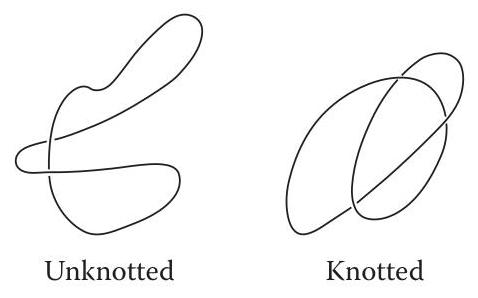
\includegraphics[max width=0.4\textwidth]{images/bo_d4b9jf3ef24c73e0334g_420_194_193_478_298_0.jpg}
\end{center}
\hspace*{3em} 

图 5-38

定理 4 (Fary-Milnor).打结的简单闭合曲线的总曲率大于 \({4\pi }\) .

证明.设 \(C = \alpha \left( \left\lbrack  {0,l}\right\rbrack  \right)\) ，设 \(T\) 是 \(\alpha\) 的一个管，设 \(R \subset  T\) 是 \(T\) 中 \(K \geq  0\) 的区域.设 \(b = b\left( s\right)\) 是 \(\alpha\) 的副法线向量，设 \(v \in  {R}^{3}\) 是一个单位向量，对于所有 \(s \in  \left\lbrack  {0,l}\right\rbrack\) ， \(v \neq   \pm  b\left( s\right)\) .设 \({h}_{v} : \left\lbrack  {0,l}\right\rbrack   \rightarrow  R\) 是 \(\alpha\) 在 \(v\) 方向上的高度函数；也就是说， \({h}_{v}\left( s\right)  = \langle \alpha \left( s\right)  - 0,v\rangle\) ， \(s \in  \left\lbrack  {0,l}\right\rbrack\) .显然， \(s\) 是 \({h}_{v}\) 的临界点当且仅当 \(v\) 垂直于 \(\alpha \left( s\right)\) 处的切线.此外，在临界点处，

\[
\frac{d}{d{s}^{2}}\left( {h}_{v}\right)  = \left\langle  {\frac{{d}^{2}\alpha }{d{s}^{2}},v}\right\rangle   = k\langle u,v\rangle  \neq  0,
\]

因为:对于所有 \(s\) 和 \(k > 0\) ， \(v \neq   \pm  b\left( s\right)\) .因此， \({h}_{v}\) 的临界点要么是极大值，要么是极小值.

现在，假设 \(\alpha\) 的总曲率小于或等于 \({4\pi }\) .这意味着

\[
{\iint }_{R}{Kd\sigma } = 2\int {kds} \leq  {8\pi }.
\]

我们声称，对于某个 \({v}_{0} \notin   \pm  b\left( \left\lbrack  {0,l}\right\rbrack  \right) ,{h}_{{v}_{0}}\) 恰好有两个临界点(因为 \(\left\lbrack  {0,l}\right\rbrack\) 是紧致的，所以这些点对应于 \({h}_{{v}_{0}}\) 的最大值和最小值).假设相反情况成立.那么，对于每一个 \(v \notin  b\left( \left\lbrack  {0,l}\right\rbrack  \right) ,{h}_{v}\) 至少有三个临界点.我们假设其中两个是极小点，即 \({s}_{1}\) 和 \({s}_{2}\) ，极大点的情况类似处理.

考虑一个平面 \(P\) 垂直于 \(v\) ，使得 \(P \cap  T = \phi\) ，并将其平行移动至 \(T\) .要么 \({h}_{v}\left( {s}_{1}\right)  = {h}_{v}\left( {s}_{2}\right)\) ，要么，比如说， \({h}_{v}\left( {s}_{1}\right)  < {h}_{v}\left( {s}_{2}\right)\) .在第一种情况下， \(P\) 在点 \({q}_{1} \neq  {q}_{2}\) 处与 \(T\) 相交，并且因为 \(v \notin  b\left( \left\lbrack  {0,l}\right\rbrack  \right) ,K\left( {q}_{1}\right)\) 和 \(K\left( {q}_{2}\right)\) 是正数.在第二种情况下，在与 \(\alpha \left( {s}_{1}\right) ,P\) 相交之前，它将在点 \({q}_{1}\) 处与 \(T\) 相交，且 \(K\left( {q}_{1}\right)  > 0\) .考虑第二个平面 \(\bar{P}\) ，它平行于 \(P\) 且距离 \(P\) 为 \(r\) ( \(r\) 是管子 \(T\) 的半径).将 \(\bar{P}\) 进一步向上移动直到它到达 \(\alpha \left( {s}_{2}\right)\) ；然后 \(P\) 将在点 \({q}_{2} \neq  {q}_{1}\) 处与 \(T\) 相交(图 5-39).因为 \({s}_{2}\) 是一个最小点且 \(v \notin  b\left( \left\lbrack  {0,l}\right\rbrack  \right) ,K\left( {q}_{2}\right)  > 0\) .在任何情况下，在 \(T\) 中都有两个不同的点满足 \(K > 0\) ，它们被 \(N\) 映射到 \({S}^{2}\) 中的一个点.这与 \({\iint }_{R}{Kd\sigma } \leq  {8\pi }\) 相矛盾，并证明了我们的主张.

\begin{center}
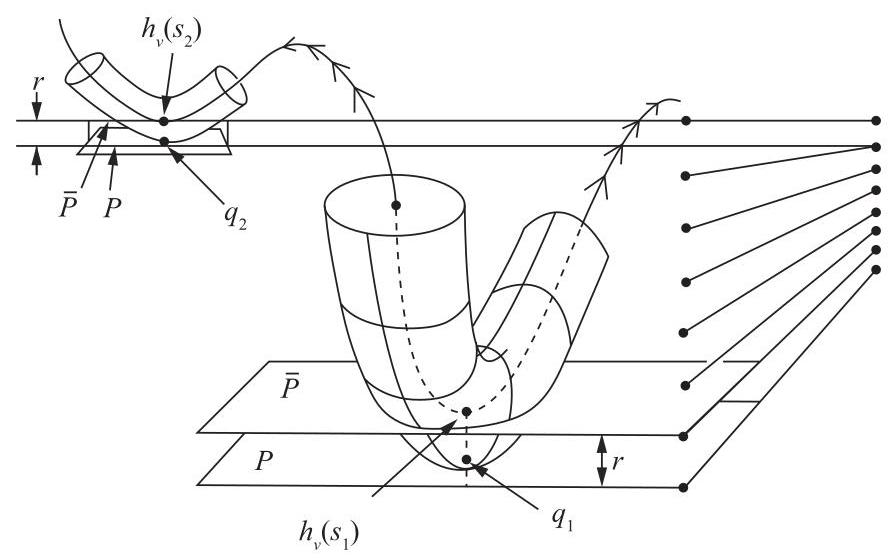
\includegraphics[max width=0.8\textwidth]{images/bo_d4b9jf3ef24c73e0334g_421_320_198_896_559_0.jpg}
\end{center}
\hspace*{3em} 

图 5-39

设 \({s}_{1}\) 和 \({s}_{2}\) 为 \({h}_{{v}_{0}}\) 的临界点，设 \({P}_{1}\) 和 \({P}_{2}\) 为垂直于 \({v}_{0}\) 并分别通过 \(\alpha \left( {s}_{1}\right)\) 和 \(\alpha \left( {s}_{2}\right)\) 的平面.介于 \({P}_{1}\) 和 \({P}_{2}\) 之间的平行于 \({v}_{0}\) 的每个平面将恰好在两个点处与 \(C\) 相交.通过线段连接这些点对，我们生成了一个由 \(C\) 界定的曲面，该曲面很容易看出与一个圆盘同胚.因此， \(C\) 是未打结的，这个矛盾完成了证明.Q.E.D.

\exerciseline

1. 确定图 5-40 中曲线 (a)、(b)、(c) 和 (d) 的旋转指数.

2. 设 \(\alpha \left( t\right)  = \left( {x\left( t\right) ,y\left( t\right) }\right) ,t \in  \left\lbrack  {0,l}\right\rbrack\) 为一可微平面闭合曲线.设 \({p}_{0} = \left( {{x}_{0},{y}_{0}}\right)  \in  {R}^{2},\left( {{x}_{0},{y}_{0}}\right)  \notin  \alpha \left( \left\lbrack  {0,l}\right\rbrack  \right)\) ，并定义函数

\[
a\left( t\right)  = \frac{x\left( t\right)  - {x}_{0}}{{\left\{  {\left( x\left( t\right)  - {x}_{0}\right) }^{2} + {\left( y\left( t\right)  - {y}_{0}\right) }^{2}\right\}  }^{1/2}},
\]

\[
b\left( t\right)  = \frac{y\left( t\right)  - {y}_{0}}{{\left\{  {\left( x\left( t\right)  - {x}_{0}\right) }^{2} + {\left( y\left( t\right)  - {y}_{0}\right) }^{2}\right\}  }^{1/2}}.
\]

a. 使用 4-4 节引理 1，证明可微函数

\[
\varphi \left( t\right)  = {\varphi }_{0} + {\int }_{0}^{t}\left( {a{b}^{\prime } - b{a}^{\prime }}\right) {dt},\;{a}^{\prime } = \frac{da}{dt},{b}^{\prime } = \frac{db}{dt},
\]

是 \(x\) 轴与位置向量 \(\left( {\alpha \left( t\right)  - {p}_{0}}\right) /\left| {\alpha \left( t\right)  - {p}_{0}}\right|\) 夹角的确定值.

\begin{center}
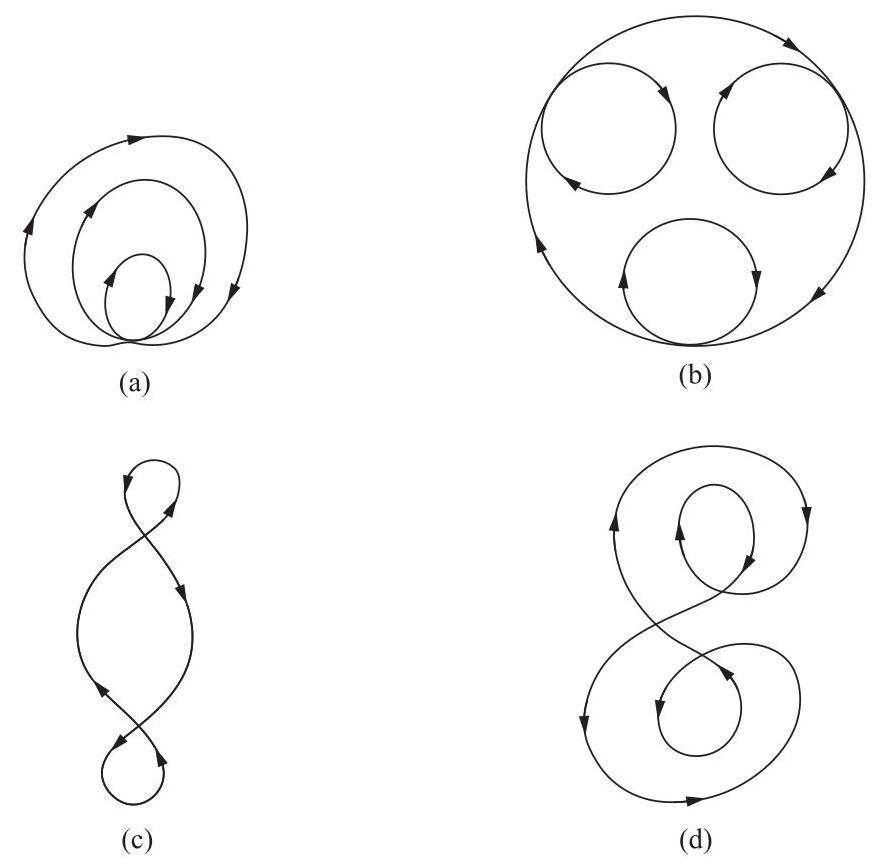
\includegraphics[max width=0.7\textwidth]{images/bo_d4b9jf3ef24c73e0334g_422_343_191_881_867_0.jpg}
\end{center}
\hspace*{3em} 

图 5-40

b. 使用 a 部分证明，当 \(\alpha\) 为可微闭合平面曲线时， \(\alpha\) 相对于 \({p}_{0}\) 的绕数由积分给出

\[
w = \frac{1}{2\pi }{\int }_{0}^{l}\left( {a{b}^{\prime } - b{a}^{\prime }}\right) {dt}.
\]

3. 令 \(\alpha  : \left\lbrack  {0,l}\right\rbrack   \rightarrow  {R}^{2}\) 和 \(\beta  : \left\lbrack  {0,l}\right\rbrack   \rightarrow  {R}^{2}\) 为两条可微的平面闭合曲线，令 \({p}_{0} \in  {R}^{2}\) 为一点，使得 \({p}_{0} \notin  \alpha \left( \left\lbrack  {0,l}\right\rbrack  \right)\) 和 \({p}_{0} \notin \; \beta \left( \left\lbrack  {0,l}\right\rbrack  \right)\) .假设对于每个 \(t \in  \left\lbrack  {0,l}\right\rbrack\) ，点 \(\alpha \left( t\right)\) 和 \(\beta \left( t\right)\) 比点 \(\alpha \left( t\right)\) 和 \({p}_{0}\) 更接近；即:

\[
\left| {\alpha \left( t\right)  - \beta \left( t\right) }\right|  < \left| {\alpha \left( t\right)  - {p}_{0}}\right| .
\]

利用习题 2 证明 \(\alpha\) 相对于 \({p}_{0}\) 的绕数等于 \(\beta\) 相对于 \({p}_{0}\) 的绕数.

4. a. 令 \(C\) 为一条正则平面闭合凸曲线.由于 \(C\) 是单的，根据若尔当曲线定理，它确定了一个内部区域 \(K \subset  {R}^{2}\) .证明 \(K\) 是一个凸集(即，给定 \(p,q \in  K\) ，直线段 \(\overline{pq}\) 包含在 \(K\) 中；参见习题 9，第 1-7 节).

b. 反之，令 \(C\) 为一条正则平面曲线(不一定是闭合的)，并假设 \(C\) 是一个凸区域的边界.证明 \(C\) 是凸的.

5. 令 \(C\) 为一条正则平面闭合凸曲线.根据习题 4， \(C\) 的内部是一个凸集 \(K\) .令 \({p}_{0} \in  K,{p}_{0} \notin  C\) .

a. 证明连接 \({p}_{0}\) 和任意点 \(q \in  C\) 的直线在 \(q\) 处不与 \(C\) 相切.

b. 从 a 部分得出， \(C\) 的旋转指数等于 \(C\) 相对于 \({p}_{0}\) 的绕数.

c. 从 b 部分得到一个简单的证明，说明闭合凸曲线的旋转指数是 \(\pm  1\) .

6. 令 \(\alpha  : \left\lbrack  {0,l}\right\rbrack   \rightarrow  {R}^{3}\) 为一条由弧长参数化的正则闭合曲线.假设对于所有 \(s \in  \left\lbrack  {0,l}\right\rbrack\) ，都有 \(0 \neq  \left| {k\left( s\right) }\right|  \leq  1\) .证明 \(l \geq  {2\pi }\) ，并且 \(l = {2\pi }\) 当且仅当 \(\alpha\) 是平面凸曲线.

7. (平面曲线的舒尔定理.)令 \(\alpha  : \left\lbrack  {0,l}\right\rbrack   \rightarrow  {R}^{2}\) 和 \(\widetilde{\alpha } : \left\lbrack  {0,l}\right\rbrack   \rightarrow \; {R}^{2}\) 为两条由弧长参数化的平面凸曲线，它们具有相同的长度 \(l\) .令 \(k\) 和 \(\widetilde{k}\) 分别为 \(\alpha\) 和 \(\widetilde{\alpha }\) 的曲率，令 \(d\) 和 \(\widetilde{d}\) 分别为 \(\alpha\) 和 \(\widetilde{\alpha }\) 的弦长；即:

\[
d\left( s\right)  = \left| {\alpha \left( s\right)  - \alpha \left( 0\right) }\right| ,\;\widetilde{d}\left( s\right)  = \left| {\widetilde{\alpha }\left( s\right)  - \widetilde{\alpha }\left( 0\right) }\right| .
\]

假设 \(k\left( s\right)  \geq  \widetilde{k}\left( s\right) ,s \in  \left\lbrack  {0,l}\right\rbrack\) .我们想证明 \(d\left( s\right)  \leq  \widetilde{d}\left( s\right)\) ， \(s \in  \left\lbrack  {0,l}\right\rbrack\) (即，如果我们拉伸一条曲线，它的弦会变长)，并且当且仅当两条曲线相差一个刚体运动时，对于 \(s \in  \left\lbrack  {0,l}\right\rbrack\) 等式成立.我们注意到，该定理可以推广到 \(\widetilde{\alpha }\) 是空间曲线的情况，并且有许多应用，参见 S. S. Chern [10].

以下大纲可能有所帮助.

a. 固定一个点 \(s = {s}_{1}\) .将两条曲线 \(\alpha \left( s\right)  = \left( {x\left( s\right) ,y\left( s\right) }\right) ,\widetilde{\alpha }\left( s\right)  = \; \left( {\widetilde{x}\left( s\right) ,\widetilde{y}\left( s\right) }\right)\) 置于下半平面 \(y \leq  0\) ，使得 \(\alpha \left( 0\right) ,\alpha \left( {s}_{1}\right) ,\widetilde{\alpha }\left( 0\right)\) ，并且 \(\widetilde{\alpha }\left( {s}_{1}\right)\) 位于 \(x\) 轴上，而 \(x\left( {s}_{1}\right)  > x\left( 0\right) ,\widetilde{x}\left( {s}_{1}\right)  > \widetilde{x}\left( 0\right)\) (参见图 5-41).设 \({s}_{0} \in  \left\lbrack  {0,{s}_{1}}\right\rbrack\) 使得 \({\alpha }^{\prime }\left( {s}_{0}\right)\) 平行于 \(x\) 轴.选择函数 \(\theta \left( s\right)\) ，它给出了 \(x\) 轴与 \({\alpha }^{\prime }\left( s\right)\) 所成角度的可微确定方式，使得 \(\theta \left( {s}_{0}\right)  = 0\) .证明，由于凸性， \(- \pi  \leq  \theta  \leq  \pi\) .

b. 设 \(\widetilde{\theta }\left( s\right) ,\widetilde{\theta }\left( {s}_{0}\right)  = 0\) 是 \(x\) 轴与 \({\alpha }^{\prime }\left( s\right)\) 所成角度的可微确定方式.(注意 \({\widetilde{\alpha }}^{\prime }\left( {s}_{0}\right)\) 可能不再平行于 \(x\) 轴.)证明 \(\widetilde{\theta }\left( s\right)  \leq  \theta \left( s\right)\) 并利用 a 部分得出

\[
d\left( {s}_{1}\right)  = {\int }_{0}^{{s}_{1}}\cos \theta \left( s\right) {ds} \leq  {\int }_{0}^{{s}_{1}}\cos \widetilde{\theta }\left( s\right) {ds} \leq  \widetilde{d}\left( {s}_{1}\right) .
\]

对于等式情况，只需追溯您的步骤并应用平面曲线的唯一性定理.

\begin{center}
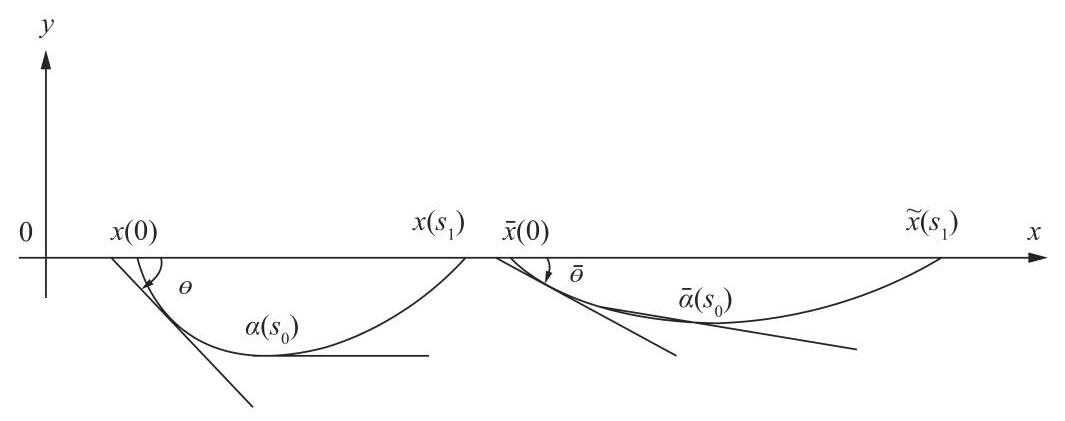
\includegraphics[max width=0.9\textwidth]{images/bo_d4b9jf3ef24c73e0334g_424_248_203_1065_421_0.jpg}
\end{center}
\hspace*{3em} 

图 5-41

8.(平面曲线的 Stoker 定理.)设 \(\alpha  : R \rightarrow  {R}^{2}\) 为由弧长参数化的正则平面曲线.假设 \(\alpha\) 满足以下条件:

1. \(\alpha\) 的曲率严格为正.

2. \(\mathop{\lim }\limits_{{s \rightarrow   \pm  \infty }}\left| {\alpha \left( s\right) }\right|  = \infty\) ；也就是说，曲线在两个方向上都延伸到无穷大.

3. \(\alpha\) 没有自交点.

本练习的目标是证明 \(\alpha\) 的总曲率为 \(\leq  \pi\) .

以下指示可能有所帮助.假设总曲率为 \(> \pi\) 且 \(\alpha\) 没有自交点.按以下步骤进行推导:

a. 证明存在点，例如 \(p = \alpha \left( 0\right) ,q = \alpha \left( {s}_{1}\right) ,{s}_{1} > 0\) ，使得在点 \(p\) 和 \(q\) 处的切线 \({T}_{p},{T}_{q}\) 分别平行，并且在弧 \(\alpha \left( \left\lbrack  {0,{s}_{1}}\right\rbrack  \right)\) 上不存在平行于 \({T}_{p}\) 的切线.

b. 表明当 \(s\) 增加时， \(\alpha \left( s\right)\) 在某点，例如 \(r\) ，处与 \({T}_{p}\) 相交(图 5-42).

c. 弧 \(\alpha \left( \left( {-\infty ,0}\right) \right)\) 必须在 \(p\) 和 \(r\) 之间的某点 \(t\) 处与 \({T}_{p}\) 相交.

d. 用一条无自交点的弧 \(\beta\) 将 \(r\) 连接到 \(t\) ，从而得到一个闭合曲线 \(C\) ，来补全 \(\alpha\) 的弧 tpqr.证明 \(C\) 的旋转指数为 \(\geq  2\) .证明这暗示 \(\alpha\) 有自交点，从而得出矛盾.

*9. 设 \(\alpha  : \left\lbrack  {0,l}\right\rbrack   \rightarrow  {S}^{2}\) 是球面 \({S}^{2} = \{ \left( {x,y,z}\right)  \in \; \left. {{R}^{3};{x}^{2} + {y}^{2} + {z}^{2} = 1}\right\}\) 上的一个正则闭合曲线.假设 \(\alpha\) 由弧长参数化，并且曲率 \(k\left( s\right)\) 处处不为零.证明

\[
{\int }_{0}^{l}\tau \left( s\right) {ds} = 0.
\]

\begin{center}
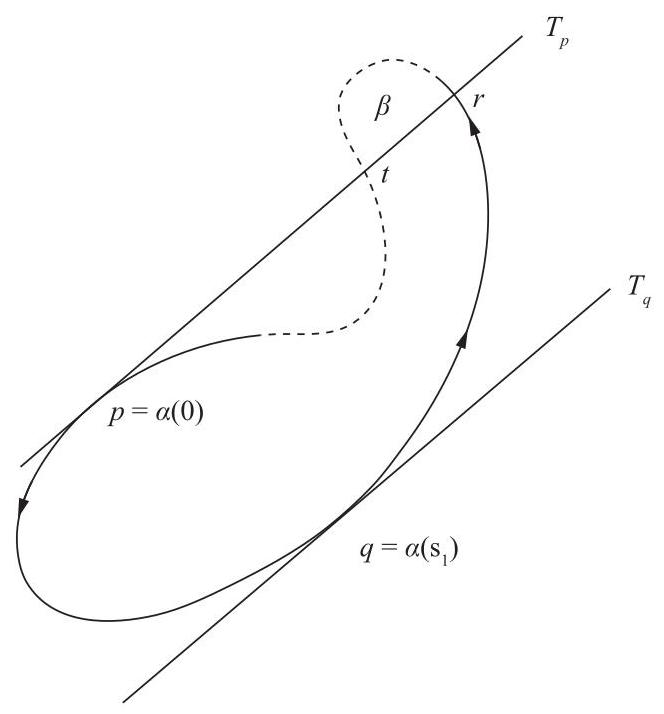
\includegraphics[max width=0.6\textwidth]{images/bo_d4b9jf3ef24c73e0334g_425_434_193_664_714_0.jpg}
\end{center}
\hspace*{3em} 

图 5-42

\section*{5-8. 高斯曲率为零的曲面}

我们已经知道(第 4-6 节)高斯曲率恒为零的正则曲面在局部上与平面等距.在本节中，我们将从它们在 \({R}^{3}\) 中的位置的角度来看待这些曲面，并证明以下全局定理.

定理. 设 \(S \subset  {\mathbb{R}}^{3}\) 是一个完备的零高斯曲率曲面.则 \(S\) 是一个圆柱面或一个平面.

根据定义，圆柱面是一个正则曲面 \(S\) ，通过该曲面的每一点 \(p \in  S\) 存在一条唯一的直线 \(R\left( p\right)  \subset  S\) (通过 \(p\) 的生成线)，该直线满足条件:如果 \(q \neq  p\) ，则直线 \(R\left( p\right)\) 和 \(R\left( q\right)\) 平行或相等.

在微分几何的历史上，这样一个定理直到其发展后期才被证明，这是一个奇怪的事实.第一个证明是 P. Hartman 和 L. Nirenberg 的一个定理(“关于雅可比行列式符号不改变的球面图像”，Amer. J. Math. 81 (1959), 901-920)的推论，该定理处理的情况比我们的情况更普遍.后来，W. S. Massey(“欧几里得空间中高斯曲率为零的曲面”，Tohoku Math. J. 14 (1962), 73-79)和 J. J. Stoker(“可展曲面”，Comm. Pure and Appl. Math. 14 (1961), 627-635)得到了该定理的初等且直接的证明.我们在此提出的证明是对

Massey 证明的修改.应该指出的是，Stoker 的论文包含一个稍微更一般的定理.

(2016年增补) I. Sabitov 教授告知我，该结果由 A.V. Pogorelov 于1956年获得.该结果发表在 Dokl. Akad. Nauk. S.S.S.R. (N.S.) 111 (1956), 945-947 题为“高斯关于球面表示定理的推广”的文章中.MR0087147.

我们将从研究零曲率曲面的一些局部性质开始.

设 \(S \subset  {R}^{3}\) 为一个高斯曲率 \(K \equiv  0\) 的正则曲面.由于 \(K = {k}_{1}{k}_{2}\) ，其中 \({k}_{1}\) 和 \({k}_{2}\) 是主曲率， \(S\) 的点是抛物点或平面点.我们用 \(P\) 表示 \(S\) 的平面点集，用 \(U = S - P\) 表示抛物点集.

\(P\) 在 \(S\) 中是闭集.事实上， \(P\) 的点满足平均曲率 \(H = \frac{1}{2}\left( {{k}_{1} + {k}_{2}}\right)\) 为零的条件.根据 \(H\) 的连续性， \(P\) 的累积点具有零平均曲率；因此，它属于 \(P\) .由此得出 \(U = S - P\) 在 \(S\) 中是开集.

以下例子给出了 \(P\) 和 \(U\) 集合之间关系的启发性示例.

例1. 考虑开三角形 \({ABC}\) ，并在其每条边上添加一个圆柱面，其母线平行于给定边(见图5-43).可以进行此构造，使得所得曲面为正则曲面.例如，为了确保在开线段 \({BC}\) 上的正则性，圆柱带 \({BCDE}\) 与垂直于 \({BC}\) 的平面相交的截面 \({FG}\) 是一个形如

\[
\exp \left( {-\frac{1}{{x}^{2}}}\right) .
\]

注意，三角形的顶点 \(A,B,C\) 和圆柱带的边 \({BE},{CD}\) 等不属于 \(S\) .

\begin{center}
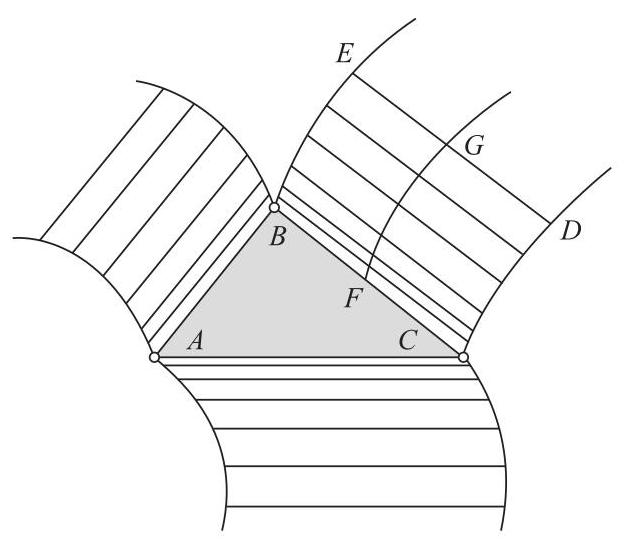
\includegraphics[max width=0.5\textwidth]{images/bo_d4b9jf3ef24c73e0334g_426_198_1566_627_546_0.jpg}
\end{center}
\hspace*{3em} 

图5-43

如此构造的曲面 \(S\) 具有曲率 \(K \equiv  0\) .集合 \(P\) 由闭三角形 \({ABC}\) 减去顶点构成.注意 \(P\) 在 \(S\) 中是闭集，但在 \({R}^{3}\) 中不是.集合 \(U\) 由圆柱带内部的点构成.通过 \(U\) 中的每一点，都存在一条唯一的直线，该直线永远不会与 \(P\) 相交. \(P\) 的边界由开线段 \({AB}\) 、 \({BC}\) 和 \({CA}\) 构成.

接下来，我们将证明这个例子中的相关性质在一般情况下也成立.

首先，设 \(p \in  U\) .由于 \(p\) 是一个抛物点， \(p\) 处的一个主方向是一个渐近方向，并且 \(p\) 处没有其他渐近方向.我们将证明通过 \(p\) 的唯一渐近曲线是一条直线段.

命题 1. 通过曲面 \(S\) 的抛物点 \(\mathrm{p} \in  \mathrm{U} \subset  S\) 的唯一渐近线，该曲面的曲率为 \(\mathrm{K} \equiv  0\) ，是 S 中(直线)的一段(开放)线段.

证明. 由于 \(p\) 不是脐线，因此可以在一个邻域 \(V \subset  U\) 中通过 \(\mathbf{x}\left( {u,v}\right)  = \mathbf{x}\) 参数化 \(p\) ，使得坐标曲线是曲率线. 假设 \(v =\) 是一个渐近曲线；也就是说，它的法曲率为零. 那么，根据 Olinde Rodrigues 定理(第 3-2 节，命题 3)，沿 \(v =\) 有 \({N}_{u} = 0\) . 由于通过邻域 \(V\) 的每一点都有一条 \(v =\) 曲线，因此关系 \({N}_{u} = 0\) 对 \(V\) 的每个点都成立.

由此可知，在 \(V\) 中

\[
\langle \mathbf{x},N{\rangle }_{u} = \left\langle  {{\mathbf{x}}_{u},N}\right\rangle   + \left\langle  {\mathbf{x},{N}_{u}}\right\rangle   = 0.
\]

因此，

\[
\langle \mathbf{x},N\rangle  = \varphi \left( v\right) , \tag{1}
\]

其中 \(\varphi \left( v\right)\) 是仅关于 \(v\) 的可微函数. 通过对式 (1) 关于 \(v\) 求导，我们得到

\[
\left\langle  {\mathbf{x},{N}_{v}}\right\rangle   = {\varphi }^{\prime }\left( v\right) . \tag{2}
\]

另一方面， \({N}_{v}\) 垂直于 \(N\) 且不为零，因为 \(V\) 的点是抛物点. 因此， \(N\) 和 \({N}_{v}\) 是线性无关的. 此外，在 \(V\) 中有 \({N}_{vu} = {N}_{uv} = 0\) .

我们现在注意到，沿曲线 \(v =\) = const. \(= {v}_{0}\) ，向量 \(N\left( u\right)  = \; {N}_{0}\) 和 \({N}_{v}\left( u\right)  = {\left( {N}_{v}\right) }_{0} =\) = const. 因此，式 (1) 表明曲线 \(\mathbf{x}\left( {u,{v}_{0}}\right)\) 属于一个垂直于常向量 \({N}_{0}\) 的平面，而式 (2) 表明该曲线属于一个垂直于常向量 \({\left( {N}_{v}\right) }_{0}\) 的平面. 因此，该曲线包含在两个平面的交集中(交集存在，因为 \({N}_{0}\) 和 \({\left( {N}_{v}\right) }_{0}\) 是线性无关的)；因此，它是线段.

Q.E.D.

注. \(K \equiv  0\) 在上述命题中是至关重要的. 例如，旋转曲面的上平行线是由抛物点组成的渐近曲线，它不是线段.

我们现在将要看看当我们扩展这条线段时会发生什么. 下面的命题表明(参见例 1)，扩展的直线永远不会与集合 \(P\) 相交；它要么在 \(S\) 的边界点“结束”，要么无限期地停留在 \(U\) 中.

使用以下术语很方便. 通过点 \(p \in  S\) 的渐近曲线称为极大的，如果它不是通过 \(p\) 的某个渐近曲线的真子集.

命题 2 (Massey, 同上). 设 \(\mathrm{r}\) 是曲面 \(S\) 的曲率为 \(\mathrm{K} \equiv  0\) 的抛物点 \(\mathrm{p} \in  \mathrm{U} \subset  S\) 的一条极大的渐近线，设 \(\mathrm{P} \subset  S\) 是 \(S\) 的平面点集. 那么 \(\mathrm{r} \cap  \mathrm{P} = \phi\) .

命题 2 的证明依赖于以下局部引理，为此我们使用 Mainardi-Codazzi 方程(参见第 4-3 节).

引理 1. 设 s 是通过曲面 \(S\) 的抛物点 \(\mathrm{p}\) 的渐近曲线的弧长，其曲率为零，设 \(\mathrm{H} = \mathrm{H}\left( S\right)\) 是 \(S\) 沿该曲线的平均曲率. 那么，在 \(\mathrm{U}\) 中，

\[
\frac{{\mathrm{d}}^{2}}{{\mathrm{\;{ds}}}^{2}}\left( \frac{1}{\mathrm{H}}\right)  = 0.
\]

引理 1 的证明.我们在 \(p\) 的邻域 \(V \subset  U\) 中引入一个坐标系 \(\left( {u,v}\right)\) ，使得坐标曲线是曲率线，并且曲线 \(v =\) = const. 是 \(V\) 的渐近线.设 \(e,f\) 和 \(g\) 是该参数化下第二基本形式的系数.由于 \(f = 0\) 和曲线 \(v =\) = const.， \(u = u\left( s\right)\) 必须满足渐近线的微分方程.

\[
e{\left( \frac{du}{ds}\right) }^{2} + {2f}\frac{du}{ds}\frac{dv}{ds} + g{\left( \frac{dv}{ds}\right) }^{2} = 0,
\]

我们得出 \(e = 0\) .在这些条件下，平均曲率 \(H\) 由下式给出:

\[
H = \frac{{k}_{1} + {k}_{2}}{2} = \frac{1}{2}\left( {\frac{e}{E} + \frac{g}{G}}\right)  = \frac{1}{2}\frac{g}{G}. \tag{3}
\]

通过将值 \(F = f = e = 0\) 代入 Mainardi-Codazzi 方程(第 4-3 节，方程 (7) 和 (7a))，我们得到:

\[
0 = \frac{1}{2}\frac{g{E}_{v}}{G},\;{g}_{u} = \frac{1}{2}\frac{g{G}_{u}}{G}. \tag{4}
\]

从 (4) 的第一个方程可知 \({E}_{v} = 0\) .因此， \(E = E\left( u\right)\) 是 \(u\) 的函数.所以，可以进行参数变换:

\[
\bar{v} = v,\;\bar{u} = \int \sqrt{E\left( u\right) }{du}.
\]

我们仍用 \(u\) 和 \(v.u\) 表示新参数，现在 \(v.u\) 表示沿 \(v =\) = const. 的弧长，因此 \(E = 1\) .

在新参数化 \(\left( {F = 0,E = 1}\right)\) 中，高斯曲率的表达式为:

\[
K =  - \frac{1}{\sqrt{G}}{\left( \sqrt{G}\right) }_{uu} = 0.
\]

因此，

\[
\sqrt{G} = {c}_{1}\left( v\right) u + {c}_{2}\left( v\right) , \tag{5}
\]

其中 \({c}_{1}\left( v\right)\) 和 \({c}_{2}\left( v\right)\) 是 \(v\) 的函数.

另一方面，(4) 的第二个方程可以写成 \(\left( {g \neq  0}\right)\) .

\[
\frac{{g}_{u}}{g} = \frac{1}{2}\frac{{G}_{u}}{\sqrt{G}\sqrt{G}} = \frac{{\left( \sqrt{G}\right) }_{u}}{\sqrt{G}};
\]

因此，

\[
g = {c}_{3}\left( v\right) \sqrt{G}, \tag{6}
\]

其中 \({c}_{3}\left( v\right)\) 是 \(v\) 的函数.将方程 (5) 和 (6) 代入方程 (3) 中，我们得到:

\[
H = \frac{1}{2}\frac{{c}_{3}\left( v\right) }{\sqrt{G}}\frac{\sqrt{G}}{\sqrt{G}} = \frac{1}{2}\frac{{c}_{3}\left( v\right) }{{c}_{1}\left( v\right) u + {c}_{2}\left( v\right) }.
\]

最后，回想一下 \(u = s\) 并对上述表达式关于 \(s\) 求导，我们得出:

\[
\frac{{d}^{2}}{d{s}^{2}}\left( \frac{1}{H}\right)  = 0 \tag{Q.E.D.}
\]

命题 2 的证明.假设通过 \(p\) 且由弧长 \(s\) 参数化的最大渐近线 \(r\) 包含一个点 \(q \in  P\) .由于 \(r\) 是连通的且 \(U\) 是开集，存在 \(r\) 中的一点 \({p}_{0}\) ，对应于 \({s}_{0}\) ，使得 \({p}_{0} \in  P\) 且 \(r\) 中具有 \(s < {s}_{0}\) 的点属于 \(U\) .

另一方面，根据引理 1，我们得出沿 \(r\) 且对于 \(s < {s}_{0}\) ，

\[
H\left( s\right)  = \frac{1}{{as} + b},
\]

其中 \(a\) 和 \(b\) 是常数.由于 \(P\) 的点具有零平均曲率，我们得到:

\[
H\left( {p}_{0}\right)  = 0 = \mathop{\lim }\limits_{{s \rightarrow  {s}_{0}}}H\left( s\right)  = \mathop{\lim }\limits_{{s \rightarrow  {s}_{0}}}\frac{1}{{as} + b},
\]

这产生了矛盾，证明完毕.Q.E.D.

设 \(\operatorname{Bd}\left( U\right)\) 是 \(U\) 在 \(S\) 中的边界；也就是说， \(\operatorname{Bd}\left( U\right)\) 是点集 \(p \in  S\) ，其中 \(S\) 中 \(p\) 的每个邻域都包含 \(U\) 中的点和 \(S - U = P\) 中的点.由于 \(U\) 在 \(S\) 中是开集，因此 \(\operatorname{Bd}\left( U\right)  \subset  P\) .此外，由于边界点的定义在 \(U\) 和 \(P\) 中是对称的，我们有

\[
\operatorname{Bd}\left( U\right)  = \operatorname{Bd}\left( P\right) .
\]

以下命题表明(正如示例 1 中一样)集合 \(\operatorname{Bd}\left( U\right)  = \operatorname{Bd}\left( P\right)\) 由直线段组成.

命题 3 (Massey).设 \(\mathrm{p} \in  {Bd}\left( \mathrm{U}\right)  \subset  S\) 是曲率为 \(\mathrm{K} \equiv  0\) 的曲面 \(S\) 的抛物点集合 \(\mathrm{U}\) 的边界点.则通过 \(\mathrm{p}\) 有一条唯一的开直线段 \(\mathrm{C}\left( \mathrm{p}\right)  \subset  S\) .此外， \(\mathrm{C}\left( \mathrm{p}\right)  \subset  {Bd}\left( \mathrm{U}\right)\) ；也就是说， \(\mathrm{U}\) 的边界由直线段组成.

证明.设 \(p \in  \operatorname{Bd}\left( U\right)\) .由于 \(p\) 是 \(U\) 的极限点，可以选择一个序列 \(\left\{  {p}_{n}\right\}  ,{p}_{n} \in  U\) ，其中 \(\mathop{\lim }\limits_{{n \rightarrow  \infty }}{p}_{n} = p\) .对于每个 \({p}_{n}\) ，设 \(C\left( {p}_{n}\right)\) 是通过 \({p}_{n}\) 的唯一的最大渐近线(开直线段)(参见命题 1).我们将证明，当 \(n \rightarrow  \infty\) 时， \(C\left( {p}_{n}\right)\) 的方向收敛于某个不依赖于序列 \(\left\{  {p}_{n}\right\}\) 选择的方向.

事实上，设 \(\sum  \subset  {R}^{3}\) 是围绕 \(p\) 的一个足够小的球面.由于球面 \(\sum\) 是紧致的， \(C\left( {p}_{n}\right)\) 与 \(\sum\) 的交点 \(\left\{  {q}_{n}\right\}\) 至少有一个累积点 \(q \in  \sum\) ，它与其对径点同时出现.如果除了 \(q\) 及其对径点之外还有另一个累积点 \(r\) ，那么通过任意接近的点 \({p}_{n}\) 和 \({p}_{m}\) 应该通过渐近线 \(C\left( {p}_{n}\right)\) 和 \(C\left( {p}_{m}\right)\) ，它们形成的夹角大于

\[
\theta  = \frac{1}{2}\operatorname{ang}\left( {{pq},{pr}}\right) ,
\]

因此与渐近线的连续性矛盾.由此可知，直线 \(C\left( {p}_{n}\right)\) 具有极限方向.类似的论证表明，这个极限方向不依赖于先前声称的具有 \(\mathop{\lim }\limits_{{n \rightarrow  \infty }}{p}_{n} = p\) 的所选序列 \(\left\{  {p}_{n}\right\}\) .

由于 \(C\left( {p}_{n}\right)\) 的方向收敛于 \({p}_{n} \rightarrow  p\) ，因此 \(C\left( {p}_{n}\right)\) 的开放线段收敛于一条穿过 \(p\) 的线段 \(C\left( p\right)  \subset  S\) .线段 \(C\left( p\right)\) 不会缩减到点 \(p\) .否则，由于 \(C\left( {p}_{n}\right)\) 是极大的， \(p \in  S\) 将是 \(C\left( {p}_{n}\right)\) 的端点的累积点，而这些端点不属于 \(S\) (参见命题 2).同理，线段 \(C\left( p\right)\) 不包含其端点.

最后，我们将证明 \(C\left( p\right)  \subset  \operatorname{Bd}\left( U\right)\) .事实上，如果 \(q \in  C\left( p\right)\) ，则存在一个序列

\[
\left\{  {q}_{n}\right\}  ,{q}_{n} \in  C\left( {p}_{n}\right)  \subset  U,\;\text{ with }\mathop{\lim }\limits_{{n \rightarrow  \infty }}{q}_{n} = q.
\]

那么 \(q \in  U \cup  \operatorname{Bd}\left( U\right)\) .假设 \(q \notin  \operatorname{Bd}\left( U\right)\) .那么 \(q \in  U\) ，并且由于渐近方向的连续性， \(C\left( p\right)\) 是穿过 \(q\) 的唯一渐近线.根据命题 2，这蕴含了 \(p \in  U\) ，这是一个矛盾.因此， \(q \in  \operatorname{Bd}\left( U\right)\) ，即 \(C\left( p\right)  \subset  \operatorname{Bd}\left( U\right)\) ，证明完毕.Q.E.D.

现在我们可以证明本节开头所述的全局结果了.

定理证明.假设 \(S\) 不是一个平面.那么(第 3-2 节，命题 4) \(S\) 包含抛物点.令 \(U\) 为 \(S\) 的抛物点(开放)集合，令 \(P\) 为 \(S\) 的平面点(闭合)集合.我们将用 int \(P\) 表示 \(P\) 的内部，即包含在 \(P\) 中的邻域的点的集合.int \(P\) 是 \(S\) 中的一个开放集，仅包含平面点.因此，int \(P\) 的每个连通分量都包含在一个平面内(第 3-2 节，命题 4).

我们首先证明，如果 \(q \in  S\) 且 \(q \notin\) int \(P\) ，则穿过 \(q\) 有一条唯一的线 \(R\left( q\right)  \subset  S\) ，并且两条这样的线要么相等要么不相交.

事实上，当 \(q \in  U\) 时，存在一条穿过 \(q.r\) 的唯一的极大切线 \(r\) ， \(q.r\) 是线段(因此是测地线)并且 \(r \cap  P = \phi\) (参见命题 1 和 2).通过按弧长参数化 \(r\) ，我们看到 \(r\) 不是有限线段.否则，存在一条无法扩展到所有参数值的测地线，这与 \(S\) 的完备性矛盾.因此， \(r\) 是一条完整的线 \(R\left( q\right)\) ，并且由于 \(r \cap  P = \phi\) ，我们得出结论 \(R\left( q\right)  \subset  U\) .由此可知，当 \(p\) 是 \(U,p \notin  R\left( q\right)\) 的另一个点时， \(R\left( p\right)  \cap  R\left( q\right)  = \phi\) .否则，应该有两条渐近线穿过交点，这与所声称的唯一性矛盾.

另一方面，如果 \(q \in  \operatorname{Bd}\left( U\right)  = \operatorname{Bd}\left( P\right)\) ，那么(参见命题 3)通过 \(q\) 有一条唯一的直线段包含在 \(\operatorname{Bd}\left( U\right)\) 中.根据前面的论证，该线段可以扩展为一条完整的直线 \(R\left( q\right)  \subset  \operatorname{Bd}\left( U\right)\) ，并且如果 \(p \in  \operatorname{Bd}\left( U\right) ,p \notin  R\left( q\right)\) ，那么 \(R\left( p\right)  \cap  R\left( q\right)  = \phi\) .

显然，由于 \(U\) 是开集，如果 \(q \in  U\) 且 \(p \in  \operatorname{Bd}\left( U\right)\) ，那么 \(R\left( p\right)  \cap  R\left( q\right)  = \phi\) .这样，通过 \(S -\) int \(P = U \cup  \operatorname{Bd}\left( U\right)\) 的每一点都有一条唯一的直线包含在 \(S\) - int \(P\) 中，并且两条这样的直线要么相等要么不相交，正如我们所声称的.我们现在声称这些直线平行于一个固定的方向，并且我们将得出结论， \(\operatorname{Bd}\left( U\right) \left( { = \operatorname{Bd}\left( P\right) }\right)\) 由平行线组成，并且 int \(P\) 的每个连通分量都是一个平面上的开集，由两条平行线界定.因此，通过 int \(P\) 的每一点 \(r \subset\) 都有一条唯一的直线 \(R\left( t\right)  \subset\) int \(P\) 平行于公共方向.由此得出，通过 \(S\) 的每一点都有一条唯一的生成线，并且生成线是平行的，也就是说， \(S\) 是一个圆柱体，正如我们所希望的.

为了证明通过 \(U \cup  \mathrm{{Bd}}\left( U\right)\) 的点的直线是平行的，我们将按以下方式进行.设 \(q \in  U \cup  \mathrm{{Bd}}\left( U\right)\) 和 \(p \in  U\) .由于 \(S\) 是连通的，存在一条弧 \(\alpha  : \left\lbrack  {0,l}\right\rbrack   \rightarrow  S\) ，其中 \(\alpha \left( 0\right)  = p,\alpha \left( l\right)  = q\) .映射 \({\exp }_{p} : {T}_{p}\left( S\right)  \rightarrow  S\) 是一个覆盖映射(命题 7，第 5-6 节)和一个局部等距(引理 1 的推论，第 5-6 节).设 \(\widetilde{\alpha } : \left\lbrack  {0,l}\right\rbrack   \rightarrow  {T}_{p}\left( S\right)\) 是 \(\alpha\) 的提升，其起点为原点 \(0 \in  {T}_{p}\left( S\right)\) .对于每个 \(\widetilde{\alpha }\left( t\right)\) ，其中 \({\exp }_{p}\widetilde{\alpha }\left( t\right)  = \; \alpha \left( t\right)  \in  U \cup  \operatorname{Bd}\left( U\right)\) ，设 \({r}_{t}\) 是 \(R\left( {\alpha \left( t\right) }\right)\) 的提升，其起点为 \(\widetilde{\alpha }\left( t\right)\) .由于 \({\exp }_{p}\) 是一个局部等距， \({r}_{t}\) 是 \({T}_{p}\left( S\right)\) 中的一条直线.

此外，当 \(\alpha \left( {t}_{1}\right)  \neq  \alpha \left( {t}_{2}\right) ,{t}_{1},{t}_{2} \in  \left\lbrack  {0,l}\right\rbrack\) 时，直线 \({r}_{{t}_{1}}\) 和 \({r}_{{t}_{2}}\) 是平行的.事实上，如果 \(v \in  {r}_{{t}_{1}} \cap  {r}_{{t}_{2}}\) ，那么

\[
{\exp }_{p}\left( v\right)  \in  R\left( {\alpha \left( {t}_{1}\right) }\right)  \cap  R\left( {\alpha \left( {t}_{2}\right) }\right) ,
\]

这是一个矛盾.这证明了我们的主张，以及定理.证毕.

\section*{5-9. 雅可比定理}

测地线 \(\gamma\) 的一个基本性质是(第 4-6 节，命题 4)，当 \(\gamma\) 上的两点 \(p\) 和 \(q\) 足够接近时， \(\gamma\) 最小化 \(p\) 和 \(q\) 之间的弧长.这意味着 \(\gamma\) 在 \(p\) 和 \(q\) 之间的弧长小于或等于连接 \(p\) 到 \(q\) 的任何曲线的弧长.现在假设我们沿着一条从点 \(p\) 开始的测地线 \(\gamma\) 行进.那么自然会问，测地线 \(\gamma\) 在多大程度上最小化了弧长.例如，在球体的情况下，从点 \(p\) 开始的测地线 \(\gamma\) (一条经线)在到达 \(p\) 相对于 \(\gamma\) 的第一个共轭点(即 \(p\) 的对跖点)之前，最小化了弧长.过了 \(p\) 的对跖点之后，测地线就不再是最小的了，正如我们可以通过以下考虑直观地看到的.

连接球体上两点 \(p\) 和 \(q\) 的测地线可以被认为是拉紧在球体上连接给定两点的线.当弧 \(\overset{\text{ ⏜ }}{pq}\) 小于半经线且点 \(p\) 和 \(q\) 保持固定时，不可能在不增加其长度的情况下移动线.另一方面，当弧 \(\overset{\text{ ⏜ }}{pq}\) 大于半经线时，线的微小位移( \(p\) 和 \(q\) 固定)会使线“松弛”(见图 5-44).换句话说，当 \(q\) 比 \(p\) 的对跖点更远时，可以得到连接 \(p\) 到 \(q\) 的曲线，这些曲线接近测地弧 \(\overbrace{pq}\) 并且比该弧短.显然，这远非一个数学论证.

在本节中，我们将开始研究这个问题，并证明一个雅可比的结果，该结果大致可以描述如下.从点 \(p\) 开始的测地线 \(\gamma\) ，相对于 \(\gamma\) 的“邻近”曲线，仅在 \(p\) 相对于 \(\gamma\) 的“第一个”共轭点之前最小化弧长(更精确的陈述将在后面给出；参见定理 1 和 2).

\begin{center}
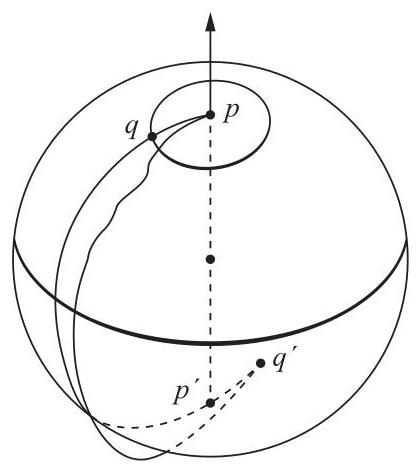
\includegraphics[max width=0.3\textwidth]{images/bo_d4b9jf3ef24c73e0334g_433_180_194_419_471_0.jpg}
\end{center}
\hspace*{3em} 

图 5-44

为简化起见，本节中的曲面假定为完整的，测地线由弧长参数化.

我们需要一些初步结果.

下面的引理表明， \({\exp }_{p} : {T}_{p}\left( S\right)  \rightarrow  S\) 在 \({T}_{p}\left( S\right)\) 的线段(起点为 \(O \in  {T}_{p}\left( S\right)\) 的测地线，从 \(p\) 开始)的像，相对于 \({\exp }_{p}\) 在连接该线段端点的 \({T}_{p}\left( S\right)\) 曲线的像，是极小的.

更精确地说，设

\[
p \in  S,\;u \in  {T}_{p}\left( S\right) ,\;l = \left| u\right|  \neq  0,
\]

设 \(\widetilde{\gamma } : \left\lbrack  {0,l}\right\rbrack   \rightarrow  {T}_{p}\left( S\right)\) 为 \({T}_{p}\left( S\right)\) 的直线，由下式给出

\[
\widetilde{\gamma }\left( s\right)  = {sv},\;s \in  \left\lbrack  {0,l}\right\rbrack  ,\;v = \frac{u}{\left| u\right| }.
\]

设 \(\widetilde{\alpha } : \left\lbrack  {0,l}\right\rbrack   \rightarrow  {T}_{p}\left( S\right)\) 为 \({T}_{p}\left( S\right)\) 的可微参数化曲线，具有 \(\widetilde{\alpha }\left( 0\right)  = 0,\widetilde{\alpha }\left( l\right)  = u\) ，以及 \(\widetilde{\alpha }\left( s\right)  \neq  0\) ，如果 \(s \neq  0\) .此外，设(图 5-45)

\[
\alpha \left( s\right)  = {\exp }_{p}\widetilde{\alpha }\left( s\right) \;\text{ and }\;\gamma \left( s\right)  = {\exp }_{p}\widetilde{\gamma }\left( s\right) .
\]

引理 1. 在上述记号下，我们有

1. \(l\left( \alpha \right)  \geq  l\left( \gamma \right)\) ，其中 \(l\left( \right)\) 表示相应曲线的弧长.

此外，如果 \(\widetilde{\alpha }\left( S\right)\) 不是 \(\left. {{\exp }_{\mathrm{p}},S \in  \lbrack 0,l)}\right\rbrack\) 的临界点，并且 \(\alpha\) 和 \(\gamma\) 的迹不同，则

2. \(l\left( \alpha \right)  > l\left( \gamma \right)\) .

\begin{center}
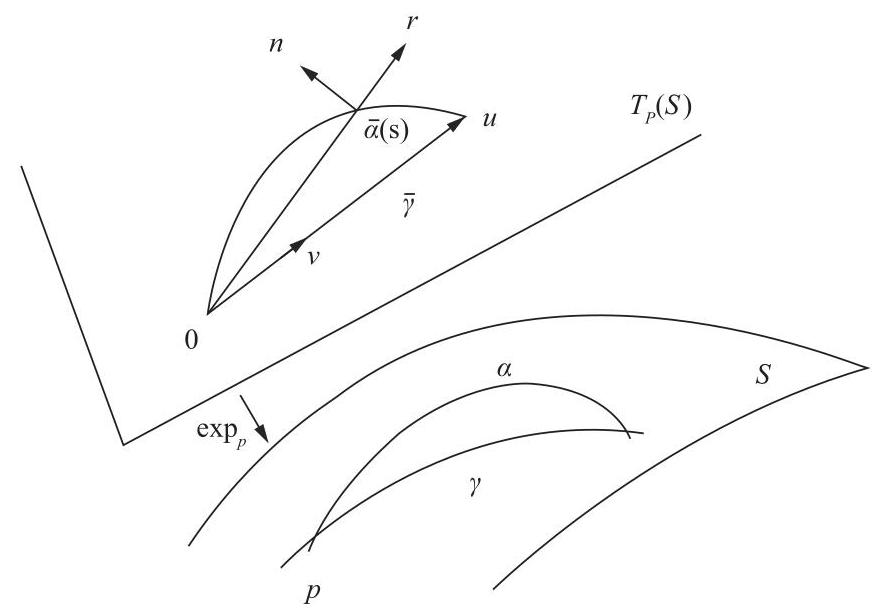
\includegraphics[max width=0.7\textwidth]{images/bo_d4b9jf3ef24c73e0334g_434_342_204_882_614_0.jpg}
\end{center}
\hspace*{3em} 

图 5-45

证明.设 \(\widetilde{\alpha }\left( s\right) /\left| {\widetilde{\alpha }\left( s\right) }\right|  = r\) ，并设 \(n\) 为 \({T}_{p}\left( S\right)\) 的单位向量，具有 \(\langle r,n\rangle  = 0\) .在 \({T}_{p}\left( S\right)\) 的基 \(\{ r,n\}\) 中，我们可以写成(图 5-45)

\[
{\widetilde{\alpha }}^{\prime }\left( s\right)  = {ar} + {bn},
\]

其中

\[
a = \left\langle  {{\widetilde{\alpha }}^{\prime }\left( s\right) ,r}\right\rangle
\]

\[
b = \left\langle  {{\widetilde{\alpha }}^{\prime }\left( s\right) ,n}\right\rangle  .
\]

根据定义

\[
{\alpha }^{\prime }\left( s\right)  = {\left( d{\exp }_{p}\right) }_{\widetilde{\alpha }\left( s\right) }\left( {{\widetilde{\alpha }}^{\prime }\left( s\right) }\right)
\]

\[
= a{\left( d{\exp }_{p}\right) }_{\widetilde{\alpha }\left( s\right) }\left( r\right)  + b{\left( d{\exp }_{p}\right) }_{\widetilde{\alpha }\left( s\right) }\left( n\right) .
\]

因此，利用高斯引理(参见第 5-5 节，引理 2)，我们得到

\[
\left\langle  {{\alpha }^{\prime }\left( s\right) ,{\alpha }^{\prime }\left( s\right) }\right\rangle   = {a}^{2} + {c}^{2},
\]

其中

\[
{c}^{2} = {b}^{2}{\left| {\left( d{\exp }_{p}\right) }_{\widetilde{\alpha }\left( s\right) }\left( n\right) \right| }^{2}.
\]

因此

\[
\left\langle  {{\alpha }^{\prime }\left( s\right) ,{\alpha }^{\prime }\left( s\right) }\right\rangle   \geq  {a}^{2}.
\]

另一方面，

\[
\frac{d}{ds}\langle \widetilde{\alpha }\left( s\right) ,\widetilde{\alpha }\left( s\right) {\rangle }^{1/2} = \frac{\left\langle  {\widetilde{\alpha }}^{\prime }\left( s\right) ,\widetilde{\alpha }\left( s\right) \right\rangle  }{\langle \widetilde{\alpha }\left( s\right) ,\widetilde{\alpha }\left( s\right) {\rangle }^{1/2}} = \left\langle  {{\widetilde{\alpha }}^{\prime }\left( s\right) ,r}\right\rangle   = a.
\]

因此，

\[
l\left( \alpha \right)  = {\int }_{0}^{l}{\left\langle  {\alpha }^{\prime }\left( s\right) ,{\alpha }^{\prime }\left( s\right) \right\rangle  }^{1/2}{ds} \geq  {\int }_{0}^{l}{ads}
\]

\[
= {\int }_{0}^{l}\frac{d}{ds}\langle \widetilde{\alpha }\left( s\right) ,\widetilde{\alpha }\left( s\right) {\rangle }^{1/2}{ds} = \left| {\widetilde{\alpha }\left( l\right) }\right|  = l = l\left( \gamma \right) ,
\]

这就证明了第一部分.

为了证明第二部分，我们假设 \(l\left( \alpha \right)  = l\left( \gamma \right)\) .那么

\[
{\int }_{0}^{l}{\left\langle  {\alpha }^{\prime }\left( s\right) ,{\alpha }^{\prime }\left( s\right) \right\rangle  }^{1/2}{ds} = {\int }_{0}^{l}{ads},
\]

并且因为

\[
{\left\langle  {\alpha }^{\prime }\left( s\right) ,{\alpha }^{\prime }\left( s\right) \right\rangle  }^{1/2} \geq  a,
\]

对于每一个 \(s \in  \left\lbrack  {0,l}\right\rbrack\) ，等式在最后一个表达式中必须成立.因此，

\[
c = \left| b\right| \left| {{\left( d{\exp }_{p}\right) }_{\widetilde{\alpha }\left( s\right) }\left( n\right) }\right|  = 0.
\]

由于 \(\widetilde{\alpha }\left( s\right)\) 不是 \({\exp }_{p}\) 的临界点，我们得出 \(b \equiv  0\) .因此，曲线 \(\widetilde{\alpha }\) 的切线都通过 \({T}_{p}\left( s\right)\) 的原点 \(O\) .因此， \(\widetilde{\alpha }\) 是一条通过 \(O\) 的 \({T}_{p}\left( S\right)\) 线.由于 \(\widetilde{\alpha }\left( l\right)  = \widetilde{\gamma }\left( l\right)\) ，直线 \(\widetilde{\alpha }\) 和 \(\widetilde{\gamma }\) 重合，这与 \(\alpha\) 和 \(\gamma\) 的轨迹不同的假设相矛盾.由此矛盾可知 \(l\left( \alpha \right)  > l\left( \gamma \right)\) ，这就证明了第二部分并结束了引理的证明.Q.E.D.

现在我们可以证明，如果测地弧不包含共轭点，它就给出了弧长的一个局部最小值.更确切地说，我们有

定理 1 (Jacobi).设 \(\gamma  : \left\lbrack  {0,l}\right\rbrack   \rightarrow  S,\gamma \left( 0\right)  = \mathrm{p}\) 为一条没有共轭点的测地线；也就是说， \({ex}{p}_{\mathrm{p}} : {\mathrm{T}}_{\mathrm{p}}\left( S\right)  \rightarrow  S\) 在 \({\mathrm{T}}_{\mathrm{p}}\left( S\right) ,S \in  \left\lbrack  {0,l}\right\rbrack\) 的 \(\widetilde{\gamma }\left( S\right)  = S{\gamma }^{\prime }\left( 0\right)\) 线上的点处是正则的.设 \(\mathrm{h} : \left\lbrack  {0,l}\right\rbrack   \times  \left( {-\epsilon ,\epsilon }\right)  \rightarrow  S\) 为 \(\gamma\) 的一个适当变分.那么

1. 存在一个 \(\delta  > 0,\delta  \leq  \epsilon\) ，使得如果 \(\mathrm{t} \in  \left( {-\delta ,\delta }\right)\) ，

\[
\mathrm{L}\left( \mathrm{t}\right)  \geq  \mathrm{L}\left( 0\right)
\]

其中 \(\mathrm{L}\left( \mathrm{t}\right)\) 是由 \({\mathrm{h}}_{\mathrm{t}}\left( S\right)  = \mathrm{h}\left( {S,\mathrm{t}}\right) .\) 给出的曲线 \({\mathrm{h}}_{\mathrm{t}} : \left\lbrack  {0,l}\right\rbrack   \rightarrow  S\) 的长度

2. 如果此外， \({\mathrm{h}}_{\mathrm{t}}\) 的轨迹与 \(\gamma ,\mathrm{L}\left( \mathrm{t}\right)  > \mathrm{L}\left( 0\right)\) 的轨迹不同.

证明.证明本质上是表明，对于每一个 \(t \in  \left( {-\delta ,\delta }\right)\) ，都可以将曲线 \({h}_{t}\) 提升为 \({T}_{p}\left( S\right)\) 中的曲线 \({\widetilde{h}}_{t}\) ，使得 \({\widetilde{h}}_{t}\left( 0\right)  = 0,{\widetilde{h}}_{t}\left( l\right)  = \widetilde{\gamma }\left( l\right)\) ，然后应用引理 1.

由于 \({\exp }_{p}\) 在 \({T}_{p}\left( S\right)\) 的 \(\widetilde{\gamma }\) 直线上是正则的，对于每个 \(s \in  \left\lbrack  {0,l}\right\rbrack\) ，都存在 \(\widetilde{\gamma }\left( s\right)\) 的一个邻域 \({U}_{s}\) ，使得 \({\exp }_{p}\) 在 \({U}_{s}\) 上的限制是一个微分同胚.族 \(\left\{  {U}_{s}\right\}  ,s \in  \left\lbrack  {0,l}\right\rbrack\) 覆盖了 \(\widetilde{\gamma }\left( \left\lbrack  {0,l}\right\rbrack  \right)\) ，并且由于紧致性，可以得到一个有限子族，例如 \({U}_{1},\ldots ,{U}_{n}\) ，它仍然覆盖 \(\widetilde{\gamma }\left( \left\lbrack  {0,l}\right\rbrack  \right)\) .因此，我们可以通过点来划分区间 \(\left\lbrack  {0,l}\right\rbrack\)

\[
0 = {s}_{1} < {s}_{2} < \cdots  < {s}_{n} < {s}_{n + 1} = l
\]

使得 \(\widetilde{\gamma }\left( \left\lbrack  {{s}_{i},{s}_{i + 1}}\right\rbrack  \right)  \subset  {U}_{i},i = 1,\ldots ,n\) .由于 \(h\) 是连续的，而 \(\left\lbrack  {{s}_{i},{s}_{i + 1}}\right\rbrack\) 是紧致的，存在 \({\delta }_{i} > 0\) 使得

\[
h\left( {\left\lbrack  {{s}_{i},{s}_{k + 1}}\right\rbrack   \times  \left( {-{\delta }_{i},{\delta }_{i}}\right) }\right)  \subset  {\exp }_{p}\left( {U}_{i}\right)  = {V}_{i}.
\]

设 \(\delta  = \min \left( {{\delta }_{1},\ldots ,{\delta }_{n}}\right)\) .对于 \(t \in  \left( {-\delta ,\delta }\right)\) ，曲线 \({h}_{t} : \left\lbrack  {0,l}\right\rbrack   \rightarrow  S\) 可以被提升为一条曲线 \({\widetilde{h}}_{t} : \left\lbrack  {0,l}\right\rbrack   \rightarrow  {T}_{p}\left( S\right)\) ，其起点为 \({\widetilde{h}}_{t}\left( 0\right)  = 0\) ，方法如下.设 \(s \in  \left\lbrack  {{s}_{1},{s}_{2}}\right\rbrack\) .则

\[
{\widetilde{h}}_{t}\left( s\right)  = {\exp }_{p}^{-1}\left( {{h}_{t}\left( s\right) }\right) ,
\]

其中 \({\exp }_{p}^{-1}\) 是 \({\exp }_{p} : {U}_{1} \rightarrow  {V}_{1}\) 的逆映射.通过应用我们用于覆盖空间的技术(参见命题 2，第 5-6 节)，我们可以将 \({\widetilde{h}}_{t}\) 推广到所有 \(s \in  \left\lbrack  {0,l}\right\rbrack\) 并得到 \({\widetilde{h}}_{t}\left( l\right)  = \widetilde{\gamma }\left( l\right)\) .

这样，我们得出结论 \(\gamma \left( s\right)  = {\exp }_{p}\widetilde{\gamma }\left( s\right)\) 并且 \({h}_{t}\left( s\right)  = \; {\exp }_{p}{\widetilde{h}}_{t}\left( s\right) ,t \in  \left( {-\delta ,\delta }\right)\) ，其中 \({\widetilde{h}}_{t}\left( 0\right)  = 0,{\widetilde{h}}_{t}\left( l\right)  = \widetilde{\gamma }\left( l\right)\) .然后我们将引理 1 应用于这种情况并得出所需的结论.Q.E.D.

注 1. 一个不包含共轭点的测地线 \(\gamma\) 可能不是相对于不在 \(\gamma\) 邻域内的曲线的极小值.例如，在圆柱体(没有共轭点)中会出现这种情况，读者通过观察圆柱体的闭合测地线很容易验证这一点.

这种情况与共轭点只告诉我们指数映射的微分，即相邻测地线相对于给定测地线的“散开”速率有关.另一方面，测地线的全局行为由指数映射本身控制，即使其微分处处非奇异，它也可能不是全局一对一的.

另一个(这次是单连通的)发生相同情况的例子是椭球体，读者可以通过观察第 5-5 节(图 5-19)中的椭球体图形来验证.

对于从 \(p\) 开始的测地线停止全局最小化弧长(称为 \(p\) 的截断轨迹)的点的轨迹的研究，对于微分几何的某些全局定理具有根本重要性，但本书不考虑.

现在我们将继续证明包含共轭点的测地线 \(\gamma\) 不是弧长的局部最小值；也就是说，“任意接近” \(\gamma\) 都存在一条连接其端点的曲线，其长度小于 \(\gamma\) 的长度.

我们将需要一些预备知识，其中第一个是将测地线变分的定义扩展到允许分段可微函数的情况.

定义 1. 令 \(\gamma  : \left\lbrack  {0,l}\right\rbrack   \rightarrow  S\) 为 \(S\) 的一条测地线，令

\[
\mathrm{h} : \left\lbrack  {0,l}\right\rbrack   \times  \left( {-\epsilon ,\epsilon }\right)  \rightarrow  S
\]

为连续映射，其中

\[
\mathrm{h}\left( {S,0}\right)  = \gamma \left( S\right) ,\;S \in  \left\lbrack  {0,l}\right\rbrack  .
\]

\(\mathrm{h}\) 被认为是 \(\gamma\) 的一个破坏性变体，如果存在一个分区

\[
0 = {S}_{0} < {S}_{1} < {S}_{2} < \cdots  < {S}_{N - 1} < {S}_{N} = l
\]

使得 \(\left\lbrack  {0,l}\right\rbrack\) 的

\[
\mathrm{h} : \left\lbrack  {{S}_{\mathrm{i}},{S}_{\mathrm{i} + 1}}\right\rbrack   \times  \left( {-\epsilon ,\epsilon }\right)  \rightarrow  S,\;\mathrm{i} = 0,1,\ldots ,N - 1,
\]

是可微的.如果对于每个 \(\mathrm{t} \in  \left( {-\epsilon ,\epsilon }\right)\) 都有 \(\mathrm{h}\left( {0,\mathrm{t}}\right)  = \gamma \left( 0\right)\) , \(\mathrm{h}\left( {l,\mathrm{t}}\right)  = \gamma \left( l\right)\) ，则称该分段变分为真分段变分.

变分的曲线 \({h}_{t}\left( s\right) ,s \in  \left\lbrack  {0,l}\right\rbrack\) 现在是分段可微曲线.变分向量场 \(V\left( s\right)  = \left( {\partial h/\partial t}\right) \left( {s,0}\right)\) 是沿 \(\gamma\) 的分段可微向量场；也就是说， \(V : \left\lbrack  {0,l}\right\rbrack   \rightarrow  {R}^{3}\) 是一个连续映射，在每个 \(\left\lbrack  {{t}_{i},{t}_{i + 1}}\right\rbrack\) 中可微.如果 \(\left\langle  {V\left( s\right) ,{\gamma }^{\prime }\left( s\right) }\right\rangle   = 0,s \in  \left\lbrack  {0,l}\right\rbrack\) ，则称分段变分 \(h\) 为正交变分.

以完全类似于第 5-4 节命题 1 的方式，可以证明沿 \(\gamma\) 的分段可微向量场 \(V\) 会产生 \(\gamma\) 的分段变分，其变分场为 \(V\) .此外，如果

\[
V\left( 0\right)  = V\left( l\right)  = 0,
\]

则可以选择该变分为真分段变分.

类似地，函数 \(L : \left( {-\epsilon ,\epsilon }\right)  \rightarrow  R\) (变分曲线的弧长)定义为

\[
L\left( t\right)  = \mathop{\sum }\limits_{0}^{{n - 1}}{\int }_{{s}_{i}}^{{s}_{i + 1}}\left| {\frac{\partial h}{\partial s}\left( {s,t}\right) }\right| {ds}
\]

\[
= {\int }_{0}^{l}\left| {\frac{\partial h}{\partial s}\left( {s,t}\right) }\right| {ds}.
\]

根据第 5-4 节引理 1，该和的每个加数在 0 的邻域内是可微的.因此，如果 \(\delta\) 足够小，则 \(L\) 在 \(\left( {-\delta ,\delta }\right)\) 中是可微的.

第二条弧长变分 \(\left( {{L}^{\prime \prime }\left( 0\right) }\right)\) 的表达式，对于适当的以及正交的断裂变分，与第 5-4 节命题 4 中得到的结果完全相同，这很容易验证.因此，如果 \(V\) 是沿测地线 \(\gamma  : \left\lbrack  {0,l}\right\rbrack   \rightarrow  S\) 的分段可微向量场，则

\[
\left\langle  {V\left( s\right) ,{\gamma }^{\prime }\left( s\right) }\right\rangle   = 0,\;S \in  \left\lbrack  {0,l}\right\rbrack  ,\;\text{ and }\;V\left( 0\right)  = V\left( l\right)  = 0,
\]

我们有

\[
{L}_{V}^{\prime \prime }\left( 0\right)  = {\int }_{0}^{l}\left( {\left\langle  {\frac{DV}{ds},\frac{DV}{ds}}\right\rangle   - K\left( s\right) \langle V\left( s\right) ,V\left( s\right) \rangle }\right) {ds}.
\]

现在设 \(\gamma  : \left\lbrack  {0,l}\right\rbrack   \rightarrow  S\) 为一条测地线，并设 \(\mathfrak{U}\) 为沿 \(\gamma\) 的分段可微向量场集合，这些向量场与 \(\gamma\) 正交；也就是说，如果 \(V \in  \mathfrak{U}\) ，则对于所有 \(s \in  \left\lbrack  {0,l}\right\rbrack\) ，都有 \(\left\langle  {V\left( s\right) ,{\gamma }^{\prime }\left( s\right) }\right\rangle   = 0\) .注意到， \(\mathfrak{U}\) 加上自然的加法和实数乘法运算，构成一个向量空间.定义一个映射 \(I : \mathfrak{U} \times  \mathfrak{U} \rightarrow  R\) 为

\[
I\left( {V,W}\right)  = {\int }_{0}^{l}\left( {\left\langle  {\frac{DV}{ds},\frac{DW}{ds}}\right\rangle   - K\left( s\right) \langle V\left( s\right) ,W\left( s\right) \rangle }\right) {ds},
\]

其中 \(V,W \in  \mathfrak{U}\) .

可以立即验证 \(I\) 是一个对称双线性映射；也就是说， \(I\) 在每个变量上都是线性的，并且 \(I\left( {V,W}\right)  = I\left( {W,V}\right)\) .因此， \(I\) 确定了一个 \(\mathfrak{U}\) 中的二次型，由 \(I\left( {V,V}\right)\) 给出.这个二次型称为 \(\gamma\) 的指标形式.

备注 2. M. Morse 引入了测地线的指数形式，并证明了以下结果.设 \(\gamma \left( {s}_{0}\right)\) 是相对于测地线 \(\gamma  : \left\lbrack  {0,l}\right\rbrack   \rightarrow  S,{s}_{0} \in  \left\lbrack  {0,l}\right\rbrack\) 的 \(\gamma \left( 0\right)  = \; p\) 的共轭点.共轭点 \(\gamma \left( {s}_{0}\right)\) 的重数是 \({T}_{p}\left( S\right)\) 中最大的子空间 \(E\) 的维数，使得对于每一个 \(u \in  E\) 都有 \({\left( d{\exp }_{p}\right) }_{\gamma \left( {s}_{0}\right) }\left( u\right)  = 0\) .向量空间 \(E\) 中二次型 \(Q : E \rightarrow  R\) 的指数是 \(E\) 的子空间 \(L\) 的最大维数，使得 \(Q\left( u\right)  < 0,u \in  L\) .用这个术语，Morse 指数定理陈述如下:设 \(\gamma  : \left\lbrack  {0,l}\right\rbrack   \rightarrow  S\) 是一个测地线.那么 \(\gamma\) 的二次型 I 的指数是有限的，并且它等于 \(\gamma (\left( {0,l\rbrack }\right)\) 中 \(\gamma \left( 0\right)\) 的共轭点的数量，每个共轭点都计入其重数.该定理的证明可以在 J. Milnor, Morse Theory, Annals of Mathematics Studies, Vol. 51, Princeton University Press, Princeton, N. J., 1963 中找到.

为了我们的目的，我们只需要以下引理.

引理 2. 设 \(\mathrm{V} \in  \mathfrak{U}\) 是沿测地线 \(\gamma  : \left\lbrack  {0,l}\right\rbrack   \rightarrow  S\) 的 Jacobi 场，以及 \(\mathrm{W} \in  \mathfrak{U}\) .则

\[
\mathrm{I}\left( {\mathrm{V},\mathrm{W}}\right)  = \left\langle  {\frac{DV}{\mathrm{\;{ds}}}\left( l\right) ,\mathrm{W}\left( l\right) }\right\rangle   - \left\langle  {\frac{\mathrm{{DV}}}{\mathrm{{ds}}}\left( 0\right) ,\mathrm{W}\left( 0\right) }\right\rangle  .
\]

证明. 通过观察到

\[
\frac{d}{ds}\left\langle  {\frac{DV}{ds},W}\right\rangle   = \left\langle  {\frac{{D}^{2}V}{d{s}^{2}},W}\right\rangle   + \left\langle  {\frac{DV}{ds},\frac{DW}{ds}}\right\rangle  ,
\]

我们可以将 \(I\) 写成 (参见 Remark 4, Sec. 5-4) 的形式

\[
I\left( {V,W}\right)  = {\left. \left\langle  \frac{DV}{ds},W\right\rangle  \right| }_{0}^{l} - {\int }_{0}^{l}\left( \left\langle  {\frac{{D}^{2}V}{d{s}^{2}} + K\left( s\right) V\left( s\right) ,W\left( s\right) }\right\rangle  \right) {ds}.
\]

根据 \(V\) 是与 \(\gamma\) 正交的 Jacobi 场这一事实，我们得出第二项的被积函数为零.因此，

\[
I\left( {V,W}\right)  = \left\langle  {\frac{DV}{ds}\left( l\right) ,W\left( l\right) }\right\rangle   - \left\langle  {\frac{DV}{ds}\left( 0\right) ,W\left( 0\right) }\right\rangle  . \tag{Q.E.D.}
\]

现在我们可以证明:

定理 2 (Jacobi).如果我们设 \(\gamma  : \left\lbrack  {0,l}\right\rbrack   \rightarrow  S\) 是 \(S\) 的测地线，并且设 \(\gamma \left( {S}_{0}\right)  \in  \gamma \left( \left( {0,l}\right) \right)\) 是相对于 \(\gamma\) 与 \(\gamma \left( 0\right)  = \mathrm{p}\) 共轭的点，则存在 \(\gamma\) 的一个适当的断裂变分 \(\mathrm{h} : \left\lbrack  {0,l}\right\rbrack   \times  \left( {-\epsilon ,\epsilon }\right)  \rightarrow  S\) 和一个实数 \(\delta  > 0,\delta  \leq  \epsilon\) ，使得如果 \(\mathrm{t} \in  \left( {-\delta ,\delta }\right) ,t \neq  0\) ，则有 \(\mathrm{L}\left( \mathrm{t}\right)  < \mathrm{L}\left( 0\right)\) .

证明.由于 \(\gamma \left( {s}_{0}\right)\) 是相对于 \(\gamma\) 与 \(p\) 共轭的，存在一个沿 \(\gamma\) 的非零 Jacobi 场 \(J\) ，且 \(J\left( 0\right)  = J\left( {s}_{0}\right)  = 0\) .根据 Sec. 5-5 的 Prop. 4，得出 \(\left\langle  {J\left( s\right) ,{\gamma }^{\prime }\left( s\right) }\right\rangle   = 0,s \in  \left\lbrack  {0,l}\right\rbrack\) .此外， \(\left( {{DJ}/{ds}}\right) \left( {s}_{0}\right)  \neq  0\) ；否则， \(J\left( s\right)  \equiv  0\) .

现在设 \(\bar{Z}\) 是沿 \(\gamma\) 的平行向量场，且 \(\bar{Z}\left( {s}_{0}\right)  =  - \left( {{DJ}/{ds}}\right) \left( {s}_{0}\right)\) ，并且设 \(f : \left\lbrack  {0,l}\right\rbrack   \rightarrow  R\) 是一个可微函数，满足 \(f\left( 0\right)  = f\left( l\right)  = 0\) ， \(f\left( {s}_{0}\right)  = 1\) .定义 \(Z\left( s\right)  = f\left( s\right) \bar{Z}\left( s\right) ,s \in  \left\lbrack  {0,l}\right\rbrack\) .

对于每个实数 \(\eta  > 0\) ，定义一个沿 \(\gamma\) 的向量场 \({Y}_{\eta }\) ，如下所示:

\[
{Y}_{\eta } = J\left( s\right)  + {\eta Z}\left( s\right) ,\;s \in  \left\lbrack  {0,{s}_{0}}\right\rbrack  ,
\]

\[
= {\eta Z}\left( s\right) ,\;s \in  \left\lbrack  {{s}_{0},l}\right\rbrack  .
\]

\({Y}_{\eta }\) 是一个分段可微的向量场，与 \(\gamma\) 正交.由于 \({Y}_{\eta }\left( 0\right)  = \; {Y}_{\eta }\left( l\right)  = 0\) ，它产生了一个适当的、正交的、断裂的 \(\gamma\) 变分.我们将计算 \({L}^{\prime \prime }\left( 0\right)  = I\left( {{Y}_{\eta },{Y}_{\eta }}\right)\) .

对于 0 和 \({s}_{0}\) 之间的测地线段，我们将使用 \(I\) 的双线性性质和引理 2 来得到

\[
{I}_{{s}_{0}}\left( {{Y}_{\eta },{Y}_{\eta }}\right)  = {I}_{{s}_{0}}\left( {J + {\eta Z},J + {\eta Z}}\right)
\]

\[
= {I}_{{s}_{0}}\left( {J,J}\right)  + {2\eta }{I}_{{s}_{0}}\left( {J,Z}\right)  + {\eta }^{2}{I}_{{s}_{0}}\left( {Z,Z}\right)
\]

\[
= {2\eta }\left\langle  {\frac{DJ}{ds}\left( {s}_{0}\right) ,Z\left( {s}_{0}\right) }\right\rangle   + {\eta }^{2}{I}_{{s}_{0}}\left( {Z,Z}\right)
\]

\[
=  - {2\eta }{\left| \frac{DJ}{ds}\left( {s}_{0}\right) \right| }^{2} + {\eta }^{2}{I}_{{s}_{0}}\left( {Z,Z}\right) ,
\]

其中 \({I}_{{s}_{0}}\) 表示积分在 0 和 \({s}_{0}\) 之间取值.令 \(I\) 表示 0 和 \(l\) 之间的积分，并注意到积分是可加的，我们有

\[
I\left( {{Y}_{\eta },{Y}_{\eta }}\right)  =  - {2\eta }{\left| \frac{DJ}{ds}\left( {s}_{0}\right) \right| }^{2} + {\eta }^{2}I\left( {Z,Z}\right) .
\]

现在观察到，如果 \(\eta  = {\eta }_{0}\) 足够小，则上述表达式为负.因此，通过取 \({Y}_{{\eta }_{0}}\) ，我们将得到一个适当的分段变差，其中 \({L}^{\prime \prime }\left( 0\right)  < 0\) .由于 \({L}^{\prime }\left( 0\right)  = 0\) ，这意味着 0 是 \(L\) 的局部最大点；也就是说，存在 \(\delta  > 0\) 使得如果 \(t \in  \left( {-\delta ,\delta }\right) ,t \neq  0\) ，则 \(L\left( t\right)  < L\left( 0\right) .\) Q.E.D.

注 3. Jacobi 定理是注 2 中引用的 Morse 指数定理的一个特例.实际上，指数定理证明的关键点本质上是定理 2 证明中提出的思想的延伸.

\exerciseline

1. (Bonnet 定理.) 令 \(S\) 为具有高斯曲率 \(K \geq  \delta  > 0\) 的完备曲面.根据 5-5 节的练习 5，每条测地线 \(\gamma  : \lbrack 0,\infty ) \rightarrow  S\) 在区间 \((0,\pi /\sqrt{\delta }\rbrack\) 中都有一个与 \(\gamma \left( 0\right)\) 共轭的点.使用 Jacobi 定理证明这暗示 \(S\) 是紧致的，并且直径 \(p\left( S\right)  \leq  \pi /\sqrt{\delta }\) (这给出了 5-4 节 Bonnet 定理的一个新证明).

2. (完备曲面上的线.) 测地线 \(\gamma  : \left( {-\infty ,\infty }\right)  \rightarrow  S\) 被称为线，如果它的长度实现了其任意两点之间的(内蕴)距离.

a. 证明通过完备圆柱体 \({x}^{2} + {y}^{2} = 1\) 的每一点都有一条线通过.

b. 假设 \(S\) 是具有高斯曲率 \(K > 0\) 的完备曲面.令 \(\gamma  : \left( {-\infty ,\infty }\right)  \rightarrow  S\) 为 \(S\) 上的一条测地线，令 \(J\left( s\right)\) 为沿 \(\gamma\) 的一个 Jacobi 场，由 \(\left\langle  {J\left( 0\right) ,{\gamma }^{\prime }\left( 0\right) }\right\rangle   = 0,\left| {J\left( 0\right) }\right|  = 1,{J}^{\prime }\left( 0\right)  = 0\) 给出.在 \({T}_{\gamma \left( 0\right) }\left( S\right)\) 处选择一个标准正交基 \(\left\{  {{e}_{1}\left( 0\right)  = {\gamma }^{\prime }\left( 0\right) ,{e}_{2}\left( 0\right) }\right\}\) ，并通过平行移动沿 \(\gamma\) 扩展它，以在每个 \({T}_{\gamma \left( 0\right) }\left( S\right)\) 处获得一个基 \(\left\{  {{e}_{1}\left( s\right) ,{e}_{2}\left( s\right) }\right\}\) .证明 \(J\left( s\right)  = u\left( s\right) {e}_{2}\left( s\right)\) 对于某个函数 \(u\left( s\right)\) 成立，并且 \(J\) 的 Jacobi 方程是

\[
{u}^{\prime \prime } + {Ku} = 0,\;u\left( 0\right)  = 1,\;{u}^{\prime }\left( 0\right)  = 0.
\]
 (*)

c. 将 5-5 节练习 3b 部分的比较定理推广到当前情况.利用 \(K > 0\) 的事实证明可以选择 \(\epsilon  > 0\) 足够小，使得

\[
u\left( \epsilon \right)  > 0,\;u\left( {-\epsilon }\right)  > 0,\;{u}^{\prime }\left( \epsilon \right)  < 0,\;{u}^{\prime }\left( {-\epsilon }\right)  > 0,
\]

其中 \(u\left( s\right)\) 是 \(\left( *\right)\) 的一个解.将 \(\left( *\right)\) 与

\[
{v}^{\prime \prime }\left( s\right)  = 0,\;v\left( \epsilon \right)  = u\left( \epsilon \right) ,\;{v}^{\prime }\left( \epsilon \right)  = {u}^{\prime }\left( \epsilon \right) ,\;\text{ for }s \in  \lbrack \epsilon ,\infty )
\]

以及与

\[
{w}^{\prime \prime }\left( s\right)  = 0,\;w\left( {-\epsilon }\right)  = u\left( {-\epsilon }\right) ,\;{w}^{\prime }\left( {-\epsilon }\right)  = {u}^{\prime }\left( {-\epsilon }\right) ,\;\text{ for }s \in  ( - \infty , - \epsilon \rbrack
\]

得出结论:如果 \({s}_{0}\) 足够大，则 \(J\left( s\right)\) 在区间 \(\left( {-{s}_{0},{s}_{0}}\right)\) 中有两个零点.

d. 使用上述结果证明，具有正高斯曲率的完整曲面不包含直线.

\section*{5-10. 抽象曲面；进一步的推广}

在第 5-11 节中，我们将证明一个由希尔伯特提出的定理，该定理断言不存在具有常负高斯曲率的 \({R}^{3}\) 中的完整正则曲面.

实际上，该定理的表述更强一些.为了理解希尔伯特定理的正确表述和证明，引入一个源于以下考虑的抽象几何曲面的概念将是方便的.

到目前为止，我们处理的曲面是 \({R}^{3}\) 的子集 \(S\) ，在其上可微函数有意义.我们在每个 \(p \in  S\) 处定义了一个切平面 \({T}_{p}\left( S\right)\) ，并将 \(p\) 周围的微分几何发展为对 \({T}_{p}\left( S\right)\) 变化的 अध्ययन.然而，我们已经观察到，内在几何的所有概念(高斯曲率、测地线、完备性等)仅取决于每个 \({T}_{p}\left( S\right)\) 上内积的选择.如果我们能够抽象地(即，不参考 \({R}^{3}\) )定义一个可微函数有意义的集合 \(S\) ，我们最终可能会将内在几何扩展到这样的集合.

下面的定义是我们第 2 章经验的产物.历史上，它花了很长时间才出现，可能是因为在 \({R}^{3}\) 中曲面的定义中参数变换的基本作用没有被清楚地理解.

定义 1. 抽象曲面(二维可微流形)是集合 \(S\) 以及一组从开集 \({\mathrm{U}}_{\alpha } \subset  {\mathbb{R}}^{2}\) 到 \(S\) 的一对一映射 \({\mathbf{x}}_{\alpha } : {\mathrm{U}}_{\alpha } \rightarrow  S\) ，使得

1. \(\mathop{\bigcup }\limits_{\alpha }{\mathbf{x}}_{\alpha }\left( {\mathrm{U}}_{\alpha }\right)  = S\) .

2. 对于每对 \(\alpha ,\beta\) 和 \({\mathbf{x}}_{\alpha }\left( {\mathrm{U}}_{\alpha }\right)  \cap  {\mathbf{x}}_{\beta }\left( {\mathrm{U}}_{\beta }\right)  = W \neq  \phi\) ，我们有 \({\mathbf{x}}_{\alpha }^{-1}\left( \mathrm{W}\right) ,\;{\mathbf{x}}_{\beta }^{-1}\left( \mathrm{\;W}\right)\) 是 \({R}^{2}\) 中的开集，并且 \({\mathbf{x}}_{\beta }^{-1} \circ  {\mathbf{x}}_{\alpha },{\mathbf{x}}_{\alpha }^{-1} \circ  {\mathbf{x}}_{\beta }\) 是可微映射(图 5-46).

\begin{center}
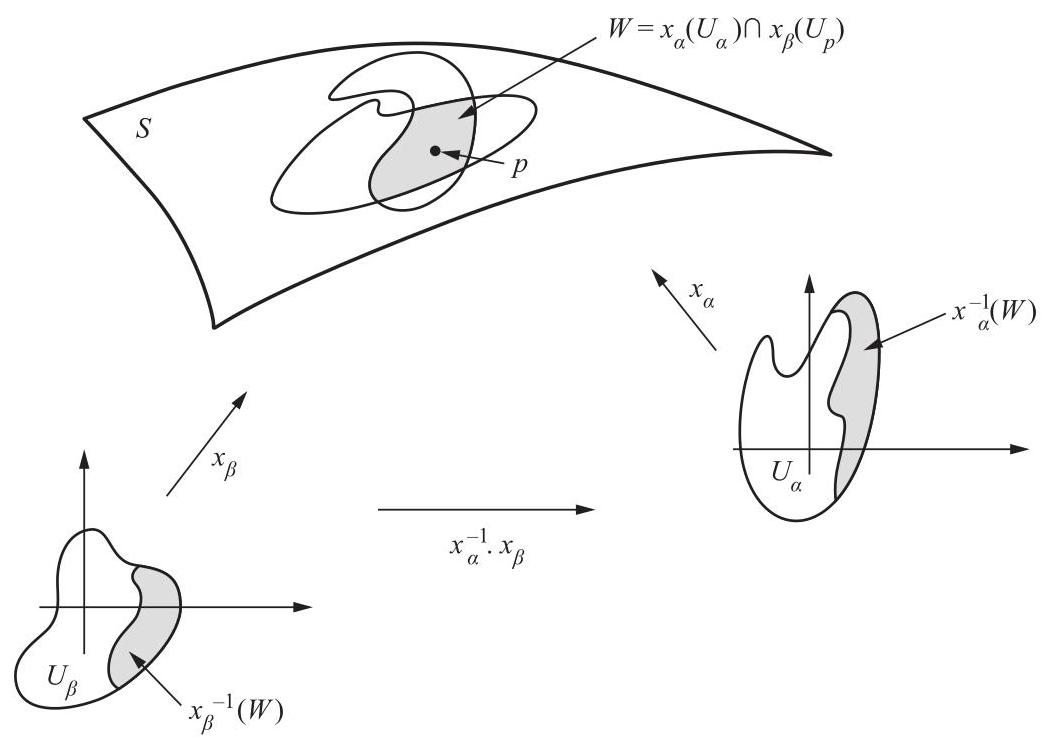
\includegraphics[max width=0.9\textwidth]{images/bo_d4b9jf3ef24c73e0334g_442_254_695_1052_742_0.jpg}
\end{center}
\hspace*{3em} 

图 5-46

一对 \(\left( {{U}_{\alpha },{\mathbf{x}}_{\alpha }}\right)\) 和 \(p \in  {\mathbf{x}}_{\alpha }\left( {U}_{\alpha }\right)\) 被称为 \(S\) 的参数化(或坐标系)，围绕 \(p.{\mathbf{x}}_{\alpha }\left( {U}_{\alpha }\right)\) 被称为坐标邻域，如果 \(q = {\mathbf{x}}_{\alpha }\left( {{u}_{\alpha },{v}_{\alpha }}\right)  \in  S\) ，我们说 \(\left( {{u}_{\alpha },{v}_{\alpha }}\right)\) 是 \(q\) 在这个坐标系中的坐标.族 \(\left\{  {{U}_{\alpha },{\mathbf{x}}_{\alpha }}\right\}\) 被称为 \(S\) 的可微结构.

我们称集合 \(V \subset  S\) 为开集，如果对于所有 \(\alpha\) ， \({\mathbf{x}}_{\alpha }^{-1}\left( V\right)\) 在 \({R}^{2}\) 中是开的.

从条件 2 可以直接得出，“参数变换”

\[
{\mathbf{x}}_{\beta }^{-1} \circ  {\mathbf{x}}_{\alpha } : {\mathbf{x}}_{\alpha }^{-1}\left( W\right)  \rightarrow  {\mathbf{x}}_{\beta }^{-1}\left( W\right)
\]

是一个微分同胚.

注 1. 有时为了方便，会在定义 1 中增加一个额外的公理，即可微结构相对于条件 1 和 2 应该是极大的.这意味着族 \(\left\{  {{U}_{\alpha },{\mathbf{x}}_{\alpha }}\right\}\) 不会被任何满足条件 1 和 2 的其他坐标邻域族所真包含.

将上述定义与 \({R}^{3}\) 中正则曲面的定义(第 2-2 节，定义 1)进行比较，可以看出关键在于将参数变换律(这是 \({R}^{3}\) 中曲面的一个定理，参见第 2-3 节，命题 1)包含在抽象曲面的定义中.由于正是这个性质使我们能够在 \({R}^{3}\) 中曲面上定义可微函数(第 2-3 节，定义 1)，因此我们可以设置

定义 2. 设 \({S}_{1}\) 和 \({S}_{2}\) 为抽象曲面.映射 \(\varphi  : {S}_{1} \rightarrow \; {S}_{2}\) 在 \(\mathrm{p} \in  {S}_{1}\) 处可微，如果给定 \(\varphi \left( \mathrm{p}\right)\) 附近的参数化 \(\mathbf{y} : \mathrm{V} \subset  {\mathbb{R}}^{2} \rightarrow  {S}_{2}\) ，存在 \(\mathrm{p}\) 附近的参数化 \(\mathbf{x} : \mathrm{U} \subset  {\mathbb{R}}^{2} \rightarrow  {S}_{1}\) ，使得 \(\varphi \left( {\mathbf{x}\left( \mathrm{U}\right) }\right)  \subset  \mathbf{y}\left( \mathrm{V}\right)\) 和映射

\[
{\mathbf{y}}^{-1} \circ  \varphi  \circ  \mathbf{x} : \mathrm{U} \subset  {\mathbb{R}}^{2} \rightarrow  {\mathbb{R}}^{2} \tag{1}
\]

在 \({\mathbf{x}}^{-1}\left( \mathrm{p}\right) .\varphi\) 处可微 在 \({S}_{1}\) 上可微，如果它在每个 \(\mathrm{p} \in  {S}_{1}\) 处可微(图 5-47).

根据条件 2，很明显，这个定义不依赖于参数化的选择.映射 (1) 称为在参数化 \(\mathbf{x},\mathbf{y}\) 中 \(\varphi\) 的表达式.

\begin{center}
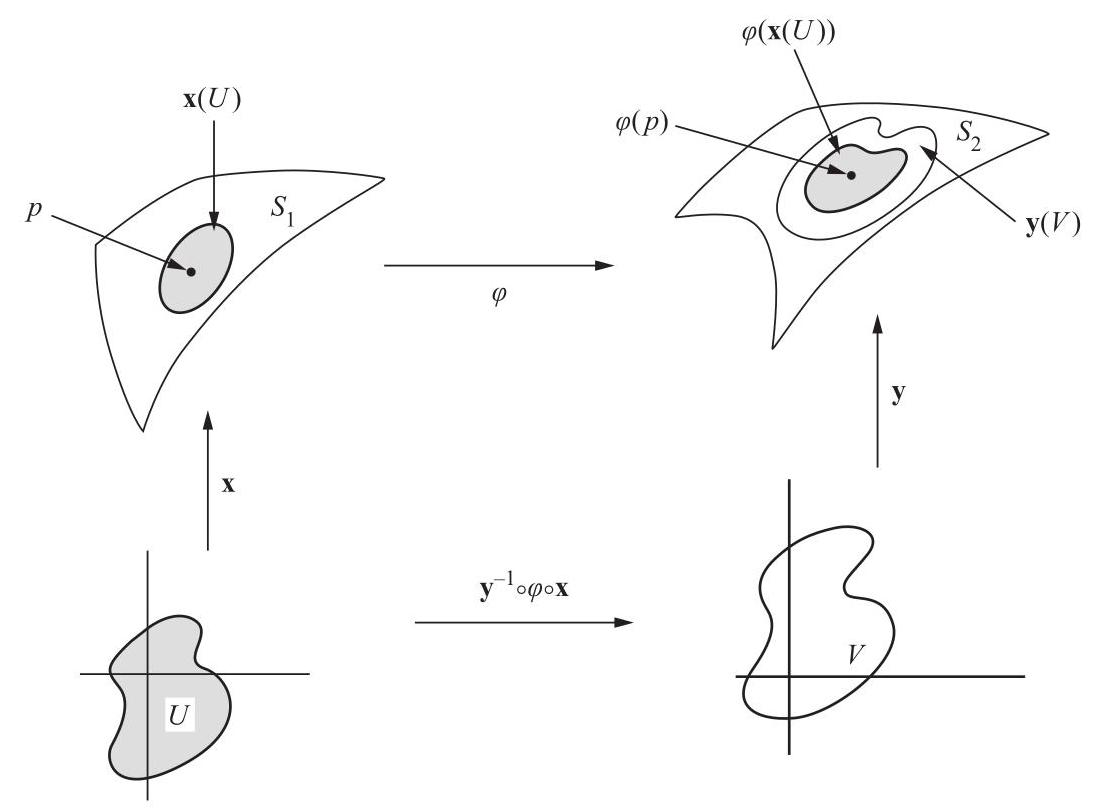
\includegraphics[max width=0.9\textwidth]{images/bo_d4b9jf3ef24c73e0334g_443_214_1233_1093_810_0.jpg}
\end{center}
\hspace*{3em} 

图 5-47

因此，在抽象曲面上讨论可微函数是有意义的，我们已经迈出了内蕴几何推广的第一步.

例 1. 设 \({S}^{2} = \left\{  {\left( {x,y,z}\right)  \in  {R}^{3};{x}^{2} + {y}^{2} + {z}^{2} = 1}\right\}\) 为单位球面，设 \(A : {S}^{2} \rightarrow  {S}^{2}\) 为对径映射；即 \(A\left( {x,y,z}\right)  = \; \left( {-x, - y, - z}\right)\) .设 \({P}^{2}\) 为通过识别 \(p\) 与 \(A\left( p\right)\) 从 \({S}^{2}\) 得到的集合，并用 \(\pi  : {S}^{2} \rightarrow  {P}^{2}\) 表示自然映射 \(\pi \left( p\right)  = \{ p,A\left( p\right) \}\) .用参数化 \({\mathbf{x}}_{\alpha } : {U}_{\alpha } \rightarrow  {S}^{2}\) 覆盖 \({S}^{2}\) ，使得 \({\mathbf{x}}_{\alpha }\left( {U}_{\alpha }\right)  \cap  A \circ  {\mathbf{x}}_{\alpha }\left( {U}_{\alpha }\right)  = \phi\) .由于 \({S}^{2}\) 是正则曲面且 \(A\) 是微分同胚，因此 \({P}^{2}\) 与族 \(\left\{  {{U}_{\alpha },\pi  \circ  {\mathbf{x}}_{\alpha }}\right\}\) 一起构成一个抽象曲面，记为 \({P}^{2}.{P}^{2}\) ，称为实射影平面.

示例 2. 令 \(T \subset  {R}^{3}\) 为一个旋转曲面(第 2-2 节，示例 4)，其圆心在 \(\left( {0,0,0}\right)  \in  {R}^{3}\) ，并令 \(A : T \rightarrow  T\) 由 \(A\left( {x,y,z}\right)  = \; \left( {-x, - y, - z}\right)\) 定义(图 5-48).令 \(K\) 为 \(T\) 关于等价关系 \(p \sim  A\left( p\right)\) 的商空间，并用 \(\pi  : T \rightarrow  K\) 表示映射 \(\pi \left( p\right)  = \{ p,A\left( p\right) \}\) .用参数化 \({\mathbf{x}}_{\alpha } : {U}_{\alpha } \rightarrow  T\) 覆盖 \(T\) ，使得 \({\mathbf{x}}_{\alpha }\left( {U}_{\alpha }\right)  \cap  A \circ  {\mathbf{x}}_{\alpha }\left( {U}_{\alpha }\right)  = \; \phi\) .与之前一样，可以证明 \(K\) 连同族 \(\left\{  {{U}_{\alpha },\pi  \circ  {\mathbf{x}}_{\alpha }}\right\}\) 是一个抽象曲面，称为克莱因瓶.

\begin{center}
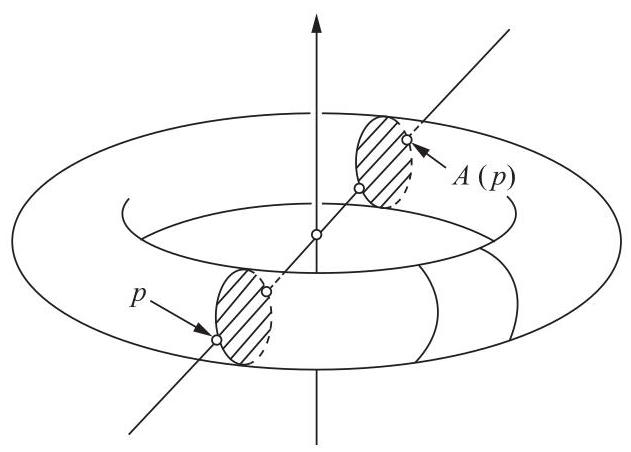
\includegraphics[max width=0.5\textwidth]{images/bo_d4b9jf3ef24c73e0334g_444_468_1103_631_452_0.jpg}
\end{center}
\hspace*{3em} 

图 5-48

现在我们需要为抽象曲面 \(S\) 的每一点关联一个切平面.再次方便地利用我们在 \({R}^{3}\) 中的曲面经验(第 2-4 节).在那里，切平面是某点处的切向量的集合，某点处的切向量被定义为曲面上某条曲线在该点的速度.因此，我们必须定义抽象曲面上曲线的切向量是什么.由于我们没有 \({R}^{3}\) 的支持，我们必须寻找一个独立于 \({R}^{3}\) 的曲线切向量的特征性质.

以下考虑将启发下面给出的定义.令 \(\alpha  : \left( {-\epsilon ,\epsilon }\right)  \rightarrow  {R}^{2}\) 为 \({R}^{2}\) 中的一个可微曲线，具有 \(\alpha \left( 0\right)  = p\) .写出 \(\alpha \left( t\right)  = \left( {u\left( t\right) ,v\left( t\right) }\right) ,t \in  \left( {-\epsilon ,\epsilon }\right)\) ，以及 \({\alpha }^{\prime }\left( 0\right)  = \left( {{u}^{\prime }\left( 0\right) ,{v}^{\prime }\left( 0\right) }\right)  = w\) .令 \(f\) 为在 \(p\) 的邻域中定义的可微函数.我们可以将 \(f\) 限制在 \(\alpha\) 上，并写出 \(f\) 相对于 \(w\) 的方向导数如下:

\[
{\left. \frac{d\left( {f \circ  \alpha }\right) }{dt}\right| }_{t = 0} = {\left. \left( \frac{\partial f}{\partial u}\frac{du}{dt} + \frac{\partial f}{\partial v}\frac{dv}{dt}\right) \right| }_{t = 0} = \left\{  {{u}^{\prime }\left( 0\right) \frac{\partial }{\partial u} + {v}^{\prime }\left( 0\right) \frac{\partial }{\partial v}}\right\}  f.
\]

因此，沿向量 \(w\) 方向的方向导数是可微函数上的一个算子，它仅取决于 \(w\) .这就是我们一直在寻找的切向量的特征性质.

定义 3. 可微映射 \(\alpha  : \left( {-\epsilon ,\epsilon }\right)  \rightarrow  S\) 称为 S 上的曲线.假设 \(\alpha \left( 0\right)  = \mathrm{p}\) ，并令 \(\mathrm{D}\) 为 \(S\) 上在 \(\mathrm{p}\) 可微的函数集合.曲线 \(\alpha\) 在 \(\mathrm{t} = 0\) 处的切向量是函数 \({\alpha }^{\prime }\left( 0\right)  : \mathrm{D} \rightarrow  \mathbb{R}\) ，其定义为

\[
{\alpha }^{\prime }\left( 0\right) \left( \mathrm{f}\right)  = {\left. \frac{\mathrm{d}\left( {\mathrm{f} \circ  \alpha }\right) }{\mathrm{{dt}}}\right| }_{t = 0},\;\mathrm{f} \in  \mathrm{D}.
\]

\(A\) 在点 \(\mathrm{p} \in  S\) 处的切向量是曲线 \(\alpha  : \left( {-\epsilon ,\epsilon }\right)  \rightarrow  S\) 在 \(\mathrm{t} = 0\) 处的一个切向量，该曲线具有 \(\alpha \left( 0\right)  = \mathrm{p}\) .

通过选择 \(p = \mathbf{x}\left( {0,0}\right)\) 附近的参数化 \(\mathbf{x} : U \rightarrow  S\) ，我们可以分别用 \(f\left( {u,v}\right)\) 和 \(\left( {u\left( t\right) ,v\left( t\right) }\right)\) 来表示 \(\mathbf{x}\) 中的函数 \(f\) 和曲线 \(\alpha\) .因此，

\[
{\alpha }^{\prime }\left( 0\right) \left( f\right)  = {\left. \frac{d}{dt}\left( f \circ  \alpha \right) \right| }_{t = 0} = {\left. \frac{d}{dt}\left( f\left( u\left( t\right) ,v\left( t\right) \right) \right) \right| }_{t = 0}
\]

\[
= {u}^{\prime }\left( 0\right) {\left( \frac{\partial f}{\partial u}\right) }_{0} + {v}^{\prime }\left( 0\right) {\left( \frac{\partial f}{\partial v}\right) }_{0}
\]

\[
= \left\{  {{u}^{\prime }\left( 0\right) {\left( \frac{\partial }{\partial u}\right) }_{0} + {v}^{\prime }\left( 0\right) {\left( \frac{\partial }{\partial v}\right) }_{0}}\right\}  \left( f\right) .
\]

这表明，给定 \(p\) 附近的坐标 \(\left( {u,v}\right)\) ，我们用 \({\left( \partial /\partial u\right) }_{0}\) 表示 \(p\) 处的切向量，它将函数 \(f\) 映射到 \({\left( \partial f/\partial u\right) }_{0}\) ；符号 \({\left( \partial /\partial v\right) }_{0}\) 也将具有类似的含义.我们注意到 \({\left( \partial /\partial u\right) }_{0}\) 和 \({\left( \partial /\partial v\right) }_{0}\) 可以被解释为“坐标曲线”在 \(p\) 处的切向量.

\[
u \rightarrow  \mathbf{x}\left( {u,0}\right) ,\;v \rightarrow  \mathbf{x}\left( {0,v}\right) ,
\]

分别(图 5-49).

由此可知， \(p\) 处的切向量集合，连同函数的 usual operations，是一个二维向量空间 \({T}_{p}\left( S\right)\) ，称为 \(S\) 在 \(p\) 处的切空间.同样可以清楚的是，选择 \(p\) 附近的参数化 \(\mathbf{x} : U \rightarrow  S\) 确定了 \({T}_{q}\left( S\right)\) 的一个相关基 \(\left\{  {{\left( \partial /\partial u\right) }_{q},{\left( \partial /\partial v\right) }_{q}}\right\}\) ，对于任何 \(q \in  \mathbf{x}\left( U\right)\) 而言.

\begin{center}
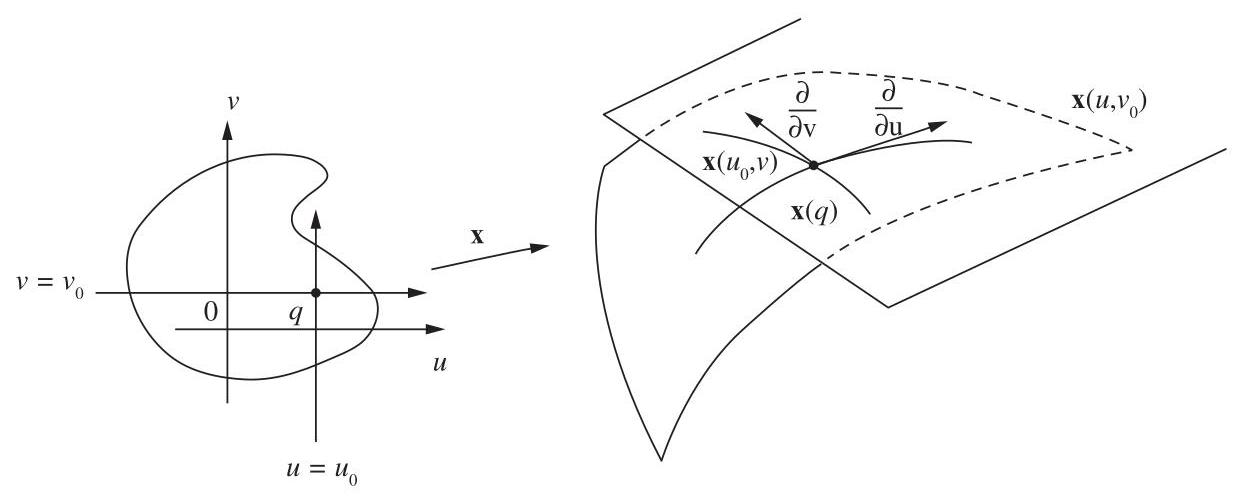
\includegraphics[max width=1.0\textwidth]{images/bo_d4b9jf3ef24c73e0334g_446_168_188_1245_498_0.jpg}
\end{center}
\hspace*{3em} 

图 5-49

有了切空间的定义，我们可以将微分的定义推广到抽象曲面.

定义 4. 令 \({S}_{1}\) 和 \({S}_{2}\) 为抽象曲面，令 \(\varphi  : {S}_{1} \rightarrow  {S}_{2}\) 为一个可微映射.对于每个 \(\mathrm{p} \in  {S}_{1}\) 和每个 \(\mathrm{w} \in  {\mathrm{T}}_{\mathrm{p}}\left( {S}_{1}\right)\) ，考虑一条可微曲线 \(\alpha  : \left( {-\epsilon ,\epsilon }\right)  \rightarrow  {S}_{1}\) ，其中 \(\alpha \left( 0\right)  = \mathrm{p},{\alpha }^{\prime }\left( 0\right)  = \mathrm{w}\) .令 \(\beta  = \varphi  \circ  \alpha\) .映射 \(\mathrm{d}{\varphi }_{\mathrm{p}} : {\mathrm{T}}_{\mathrm{p}}\left( {S}_{1}\right)  \rightarrow  {\mathrm{T}}_{\mathrm{p}}\left( {S}_{2}\right)\) 由 \(\mathrm{d}{\varphi }_{\mathrm{p}}\left( \mathrm{w}\right)  = {\beta }^{\prime }\left( 0\right)\) 定义，是一个良定义的线性映射，称为 \(\varphi\) 在 \(\mathrm{p}\) 处的微分.

\(d{\varphi }_{p}\) 是良定义且线性的证明与第 2-4 节命题 2 的证明完全相同.

现在我们可以迈出推广内蕴几何的最后一步了.

定义 5. 一个几何曲面(二维黎曼流形)是一个抽象曲面 \(S\) ，以及在每个 \({\mathrm{T}}_{\mathrm{p}}\left( S\right) ,\mathrm{p} \in  S\) 上选择一个内积 \(\langle\) , \({\rangle }_{\mathrm{p}}\) ，该内积随 \(\mathrm{p}\) 可微地变化，具体如下.对于某个(因此也是所有)围绕 \(\mathrm{p}\) 的参数化 \(\mathbf{x} : \mathrm{U} \rightarrow  S\) ，函数

\[
E\left( {u,v}\right)  = \left\langle  {\frac{\partial }{\partial u},\frac{\partial }{\partial u}}\right\rangle  ,\;F\left( {u,v}\right)  = \left\langle  {\frac{\partial }{\partial u},\frac{\partial }{\partial v}}\right\rangle  ,\;G\left( {u,v}\right)  = \left\langle  {\frac{\partial }{\partial v},\frac{\partial }{\partial v}}\right\rangle
\]

是 \(\mathrm{U}\) 中的可微函数.内积 \(\langle\) , \(\rangle {isoftencalleda}\) 是 \(S\) 上的(黎曼)度量.

现在很容易将内蕴几何的概念推广到几何曲面.事实上，对于函数 \(E,F,G\) ，我们通过 4-3 节的系统 2 为 \(S\) 定义克里斯托费尔符号.由于内蕴几何的概念都是用克里斯托费尔符号定义的，因此它们现在可以在 \(S\) 中定义.

因此，向量场沿曲线的协变导数由 4-4 节的方程 (1) 给出.平行移动的存在性源于 4-4 节的命题 2，测地线是切向量场具有零协变导数的曲线.高斯曲率可以通过 4-3 节的方程 (5) 来定义，或者如 4-5 节中所述，通过平行移动来定义.

通过以下考虑可以看出，这引入了一些新的和有趣的对象.我们将从一个与希尔伯特定理相关的例子开始.

例 3. 令 \(S = {R}^{2}\) 为一个具有坐标 \(\left( {u,v}\right)\) 的平面，并在每个点 \(q = \left( {u,v}\right)  \in  {R}^{2}\) 定义一个内积，方法是设置

\[
{\left\langle  \frac{\partial }{\partial u},\frac{\partial }{\partial u}\right\rangle  }_{q} = E = 1,\;{\left\langle  \frac{\partial }{\partial u},\frac{\partial }{\partial v}\right\rangle  }_{q} = F = 0,
\]

\[
{\left\langle  \frac{\partial }{\partial v},\frac{\partial }{\partial v}\right\rangle  }_{q} = G = {e}^{2u}.
\]

\({R}^{2}\) 具有此内积是一个几何曲面 \(H\) ，称为双曲平面. \(H\) 的几何与 \({R}^{2}\) 的通常几何不同.例如， \(H\) 的曲率为(4-3 节，练习 1)

\[
K =  - \frac{1}{2\sqrt{EG}}\left\{  {{\left( \frac{{E}_{v}}{\sqrt{EG}}\right) }_{v} + {\left( \frac{{G}_{u}}{\sqrt{EG}}\right) }_{u}}\right\}   =  - \frac{1}{2{e}^{u}}{\left( \frac{2{e}^{2u}}{{e}^{u}}\right) }_{u} =  - 1.
\]

实际上， \(H\) 的几何是洛巴切夫斯基非欧几何的一个精确模型，其中除了平行公理外，欧几里得公理都成立(参见 4-5 节).为了弄清这一点，我们将计算 \(H\) 的测地线.

如果我们查看 \(E = 1\) , \(F = 0\) (4-6 节，练习 2)时测地线的微分方程，我们立即会发现曲线 \(v =\) = 常数是测地线.为了找到其他的，定义一个映射很方便

\[
\phi  : H \rightarrow  {R}_{ + }^{2} = \left\{  {\left( {x,y}\right)  \in  {R}^{2};y > 0}\right\}
\]

由 \(\phi \left( {u,v}\right)  = \left( {v,{e}^{-u}}\right)\) 可知， \(\phi\) 是可微的，并且由于 \(y > 0\) ，它有一个可微的逆.因此， \(\phi\) 是一个微分同胚，我们可以通过设置在 \({R}_{ + }^{2}\) 中诱导一个内积

\[
{\left\langle  d\phi \left( {w}_{1}\right) ,d\phi \left( {w}_{2}\right) \right\rangle  }_{\phi \left( q\right) } = {\left\langle  {w}_{1},{w}_{2}\right\rangle  }_{q}.
\]

为了计算这个内积，我们观察到

\[
\frac{\partial }{\partial x} = \frac{\partial }{\partial v},\;\frac{\partial }{\partial y} =  - {e}^{u}\frac{\partial }{\partial u},
\]

因此，

\[
\left\langle  {\frac{\partial }{\partial x},\frac{\partial }{\partial x}}\right\rangle   = {e}^{2u} = \frac{1}{{y}^{2}},\;\left\langle  {\frac{\partial }{\partial x},\frac{\partial }{\partial y}}\right\rangle   = 0,\;\left\langle  {\frac{\partial }{\partial y},\frac{\partial }{\partial y}}\right\rangle   = \frac{1}{{y}^{2}}.
\]

\({R}_{ + }^{2}\) 具有此内积与 \(H\) 等距，有时被称为庞加莱半平面.

为了确定 \(H\) 的测地线，我们使用庞加莱半平面并进行两次进一步的坐标变换.

首先，固定一个点 \(\left( {{x}_{0},0}\right)\) 并设置(图 5-50)

\[
x - {x}_{0} = \rho \cos \theta ,\;y = \rho \sin \theta ,
\]

\begin{center}
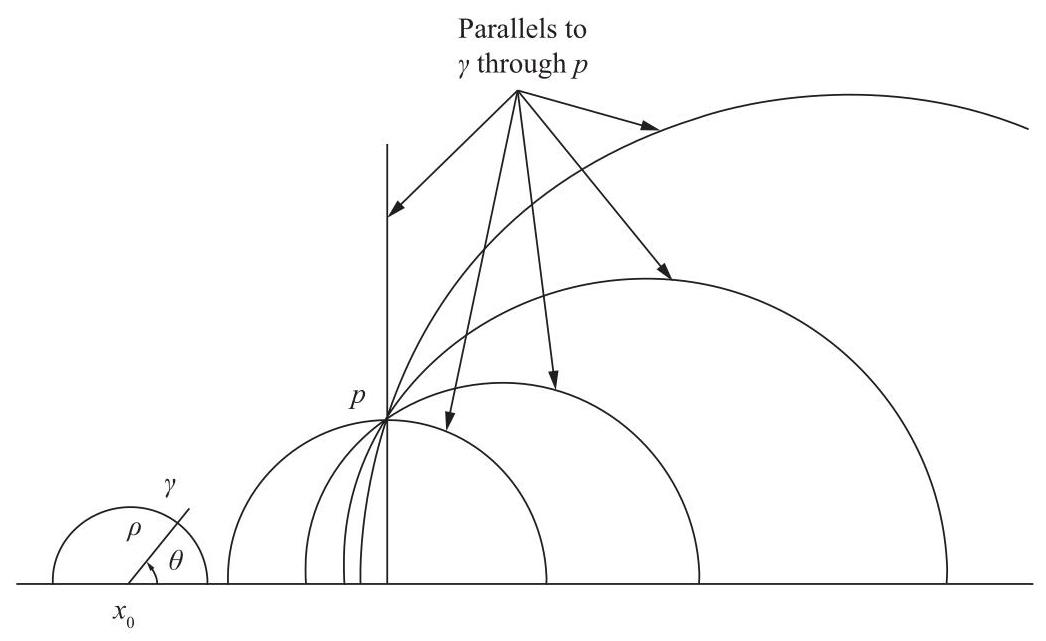
\includegraphics[max width=0.9\textwidth]{images/bo_d4b9jf3ef24c73e0334g_448_259_742_1046_641_0.jpg}
\end{center}
\hspace*{3em} 

图 5-50

\(0 < \theta  < \pi ,0 < \rho  <  + \infty\) . 这是 \({R}_{ + }^{2}\) 到自身的一个微分同胚，并且

\[
\left\langle  {\frac{\partial }{\partial \rho },\frac{\partial }{\partial \rho }}\right\rangle   = \frac{1}{{\rho }^{2}{\sin }^{2}\theta },\;\left\langle  {\frac{\partial }{\partial \rho },\frac{\partial }{\partial \theta }}\right\rangle   = 0,\;\left\langle  {\frac{\partial }{\partial \theta },\frac{\partial }{\partial \theta }}\right\rangle   = \frac{1}{{\sin }^{2}\theta }.
\]

接下来，考虑 \({R}_{ + }^{2}\) 的微分同胚，由(我们想将 \(\theta\) 变为一个参数，该参数测量 \(\rho  =\) 弧长(常数)沿)给出

\[
{\rho }_{1} = \rho ,\;{\theta }_{1} = {\int }_{0}^{\theta }\frac{1}{\sin \theta }{d\theta },
\]

得到

\[
\left\langle  {\frac{\partial }{\partial {\rho }_{1}},\frac{\partial }{\partial {\rho }_{1}}}\right\rangle   = \frac{1}{{\rho }_{1}^{2}{\sin }^{2}\theta },\;\left\langle  {\frac{\partial }{\partial {\rho }_{1}},\frac{\partial }{\partial {\theta }_{1}}}\right\rangle   = 0,\;\left\langle  {\frac{\partial }{\partial {\theta }_{1}},\frac{\partial }{\partial {\theta }_{1}}}\right\rangle   = 1.
\]

再次查看测地线的微分方程 \((F = 0\) , \(G = 1\) )，我们发现 \({\rho }_{1} = \rho  =\) 常数是测地线.(在练习 8 中给出了找到 \({R}_{ + }^{2}\) 测地线的另一种方法.)

总结我们的观察，我们得出结论，垂直于轴 \(y > 0\) 的直线和半圆是庞加莱半平面 \({R}_{ + }^{2}\) 的测地线.这些是 \({R}_{ + }^{2}\) 的所有测地线，因为通过每个点 \(q \in  {R}_{ + }^{2}\) 和从 \(q\) 发出的每个方向，要么通过一条与该直线相切且垂直于轴 \(y = 0\) 的圆，要么通过一条垂直线(当方向垂直时).

几何曲面 \({R}_{ + }^{2}\) 是完备的；也就是说，测地线可以为参数的所有值定义.这一事实的证明将留作练习(练习 7；另见练习 6).

现在很容易看出，如果我们定义 \({R}_{ + }^{2}\) 的直线为测地线，那么欧几里得公理中除平行公理外的所有公理在此几何中都成立.欧几里得平面 \(P\) 中的平行公理断言，从不在直线 \(r \subset  P\) 上的点可以画出一条唯一的直线 \({r}^{\prime } \subset  P\) ，该直线不与 \(r\) 相交.实际上，在 \({R}_{ + }^{2}\) 中，从不在测地线 \(\gamma\) 上的点可以画出无数条不与 \(\gamma\) 相交的测地线.

那么问题就出现了，是否可以在 \({R}^{3}\) 中找到这样一个曲面作为正则曲面.这个问题最自然的语境是以下定义.

定义 6. 抽象曲面 \(S\) 到 \({\mathbb{R}}^{3}\) 的可微映射 \(\varphi  : S \rightarrow  {\mathbb{R}}^{3}\) 是一个浸入，如果微分 \(\mathrm{d}{\varphi }_{\mathrm{p}} : {\mathrm{T}}_{\mathrm{p}}\left( S\right)  \rightarrow  {\mathrm{T}}_{\mathrm{p}}\left( {\mathbb{R}}^{3}\right)\) 是单射的.如果 S 还有一个度量 \(\langle \rangle\) ，则 \(\rangle {and}\)

\[
{\left\langle  \mathrm{d}{\varphi }_{\mathrm{p}}\left( \mathrm{v}\right) ,\mathrm{d}{\varphi }_{\mathrm{p}}\left( \mathrm{w}\right) \right\rangle  }_{\varphi \left( \mathrm{p}\right) } = \langle \mathrm{v},\mathrm{w}{\rangle }_{\mathrm{p}},\;\mathrm{v},\mathrm{w} \in  {\mathrm{T}}_{\mathrm{p}}\left( S\right) ,
\]

\(\varphi\) 被认为是一种等距浸入.

请注意，上述关系中的第一个内积是 \({R}^{3}\) 的通常内积，而第二个内积是 \(S\) 上给定的黎曼度量.这意味着在等距浸入中，由 \({R}^{3}\) 在 \(S\) 上“诱导”的度量与 \(S\) 上给定的度量一致.

希尔伯特定理将在 5-11 节证明，它指出不存在到 \({R}^{3}\) 的完备双曲平面的等距浸入.特别是，无法在 \({R}^{3}\) 中找到一个正则曲面作为洛巴切夫斯基几何的模型.

实际上，我们不必局限于 \({R}^{3}\) .上述等距嵌入的定义在我们将 \({R}^{3}\) 替换为 \({R}^{4}\) 或任意 \({R}^{n}\) 时是完全合理的.因此，我们可以拓宽我们最初的问题，并问:对于 \(N\) 的哪些值，存在一个从完整的双曲平面到 \({\mathbb{R}}^{N}\) 的等距嵌入？希尔伯特定理表明 \(n \geq  4\) .据我们所知， \(n = 4\) 的情况仍未解决.

因此，抽象曲面的引入带来了新的对象，并阐明了我们对重要问题的看法.

在本节的其余部分，我们将更详细地探讨一些刚刚介绍的思想，并展示它们如何自然地引出进一步的重要推广.下一节的理解将不需要这部分内容.

让我们看一些进一步的例子.

例4.设 \({R}^{2}\) 为具有坐标 \(\left( {x,y}\right)\) 的平面， \({T}_{m,n} : {R}^{2} \rightarrow \; {R}^{2}\) 为映射(平移) \({T}_{m,n}\left( {x,y}\right)  = \left( {x + m,y + n}\right)\) ，其中 \(m\) 和 \(n\) 为整数.通过 \(\left( {x,y}\right)  \sim  \left( {{x}_{1},{y}_{1}}\right)\) 在 \({R}^{2}\) 中定义一个等价关系，当且仅当存在整数 \(m,n\) 使得 \({T}_{m,n}\left( {x,y}\right)  = \left( {{x}_{1},{y}_{1}}\right)\) .设 \(T\) 为 \({R}^{2}\) 通过此等价关系的商空间，设 \(\pi  : {R}^{2} \rightarrow  T\) 为自然投影映射 \(\pi \left( {x,y}\right)  = \left\{  {{T}_{m,n}\left( {xy}\right) \text{ ; all integers }m,n}\right\}\) .因此，在顶点具有整数坐标的每个开单位正方形中，只有一个 \(T\) 的代表，并且 \(T\) 可以被看作是一个带有对边识别的闭合正方形.(参见图5-51.注意 \({R}^{2}\) 中用 \(x\) 表示的所有点在 \(T\) 中代表同一个点 \(p\) .)

设 \({i}_{\alpha } : {U}_{\alpha } \subset  {R}^{2} \rightarrow  {R}^{2}\) 为 \({R}^{2}\) 的一族参数化，其中 \({i}_{\alpha }\) 为恒等映射，使得对所有 \(m,n\) 都有 \({U}_{\alpha } \cap  {T}_{m,n}\left( {U}_{\alpha }\right)  = \phi\) .由于 \({T}_{m,n}\) 是一个微分同胚，可以很容易地检查出 \(\left( {{U}_{\alpha },\pi  \circ  {i}_{\alpha }}\right)\) 族是 \(T.T\) 的一个可微结构，称为(可微)环面.从 \(T,\pi  : {R}^{2} \rightarrow  T\) 上的可微结构的定义来看， \(T,\pi  : {R}^{2} \rightarrow  T\) 是一个可微映射和一个局部微分同胚(图5-51中的构造表明 \(T\) 与 \({R}^{3}\) 中的标准环面微分同胚).

\begin{center}
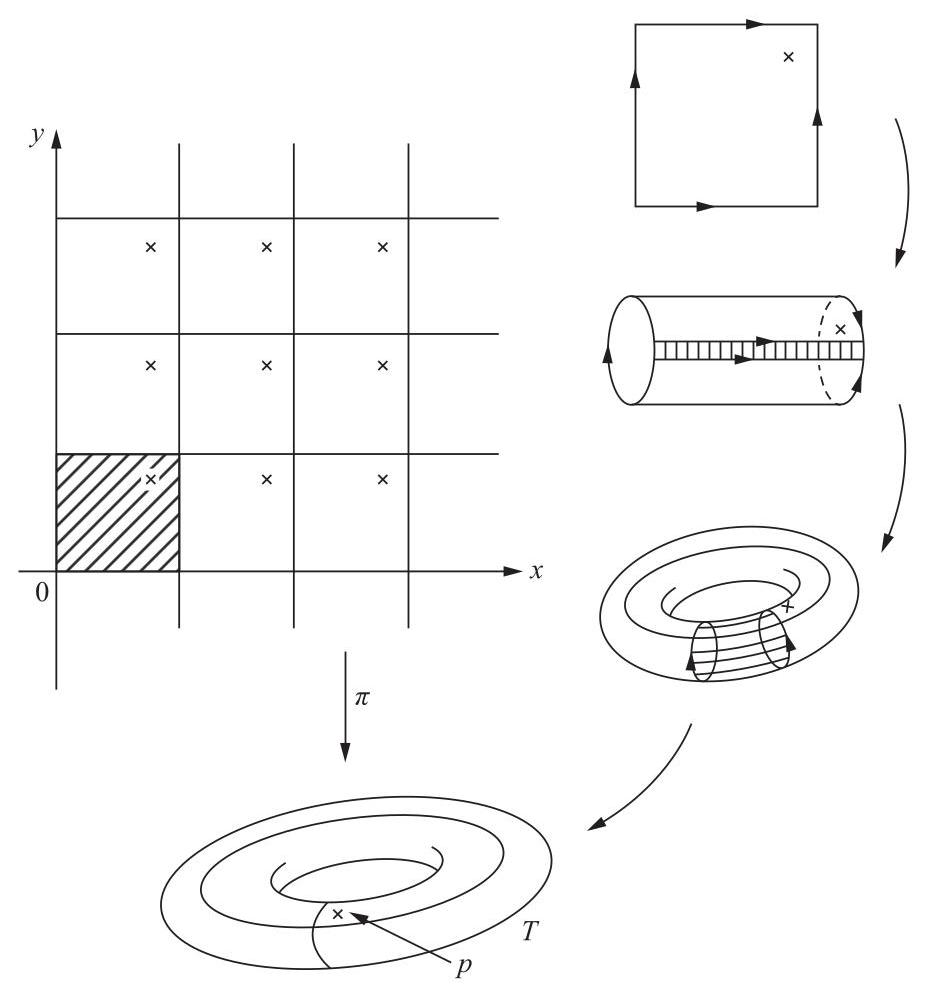
\includegraphics[max width=0.8\textwidth]{images/bo_d4b9jf3ef24c73e0334g_450_320_1049_925_990_0.jpg}
\end{center}
\hspace*{3em} 

图5-51.环面.

现在注意到 \({T}_{m,n}\) 是 \({R}^{2}\) 的等距同构，并如下在 \(T\) 上引入一个几何(黎曼)结构.设 \(p \in  T\) 和 \(v \in  {T}_{p}\left( T\right)\) .设 \({q}_{1},{q}_{2} \in  {R}^{2}\) 和 \({w}_{1},{w}_{2} \in  {R}^{2}\) 使得 \(\pi \left( {q}_{1}\right)  = \pi \left( {q}_{2}\right)  = p\) 和 \(d{\pi }_{{q}_{1}}\left( {w}_{1}\right)  = d{\pi }_{{q}_{2}}\left( {w}_{2}\right)  = v\) .那么 \({q}_{1} \sim  {q}_{2}\) ；因此，存在 \({T}_{m,n}\) 使得 \({T}_{m,n}\left( {q}_{1}\right)  = {q}_{2},d{\left( {T}_{m,n}\right) }_{{q}_{1}}\left( {w}_{1}\right)  = {w}_{2}\) .由于 \({T}_{m,n}\) 是一个等距同构， \(\left| {w}_{1}\right|  = \left| {w}_{2}\right|\) .现在，定义 \(v\) 在 \({T}_{p}\left( T\right)\) 中的长度为 \(\left| v\right|  = \left| {d{\pi }_{q}\left( {w}_{1}\right) }\right|  = \left| {w}_{1}\right|\) .根据我们所见，这是良定义的.显然，这会产生一个内积 \(\langle \;,\;{\rangle }_{p}\) ，在 \({T}_{p}\left( T\right)\) 上对于每个 \(p \in  T\) .由于这本质上是 \({R}^{2}\) 的内积，而 \(\pi\) 是一个局部微分同胚， \(\langle \;,\;{\rangle }_{p}\) 随 \(p\) 可微地变化.

观察到，在族 \(\left\{  {{U}_{\alpha },\pi  \circ  {i}_{\alpha }}\right\}\) 的任何参数化中， \(T\) 的第一基本形式的系数是 \(E = G = 1,F = 0\) .因此，这个环面在局部上表现得像欧几里得空间.例如，它的高斯曲率恒为零(参见习题 1，第 4-3 节).这解释了通常赋予 \(T\) 的“平坦环面”这个名称，以及刚刚描述的内积.

显然，平坦环面不能等距地浸入 \({R}^{3}\) 中，因为根据紧致性，它会有一个正曲率点(参见习题 16，第 3-3 节，或引理 2，第 5-2 节).然而，它可以等距地浸入 \({R}^{4}\) 中.

事实上，设 \(F : {R}^{2} \rightarrow  {R}^{4}\) 由下式给出:

\[
F\left( {x,y}\right)  = \frac{1}{2\pi }\left( {\cos {2\pi x},\sin {2\pi x},\cos {2\pi y},\sin {2\pi y}}\right) .
\]

由于对于所有 \(m,n\) 都有 \(F\left( {x + m,y + n}\right)  = F\left( {x,y}\right)\) ，我们可以通过 \(\varphi \left( p\right)  = F\left( q\right)\) 定义一个映射 \(\varphi  : T \rightarrow \; {R}^{4}\) ，其中 \(q \in  {\pi }^{-1}\left( p\right)\) .显然， \(\varphi  \circ  \pi  = F\) ，并且由于 \(\pi\) : \({R}^{2} \rightarrow  T\) 是局部微分同胚，所以 \(\varphi\) 是可微的.此外， \({d\varphi }\) 的秩等于 \({dF}\) 的秩，容易计算出该秩为 2.因此， \(\varphi\) 是一个浸入.为了证明该浸入是等距的，我们首先观察到，如果 \({e}_{1} = \left( {1,0}\right) ,{e}_{2} = \left( {0,1}\right)\) 是 \({R}^{2}\) 中标准基的向量，那么向量 \(d{\pi }_{q}\left( {e}_{1}\right)  = {f}_{1},d{\pi }_{q}\left( {e}_{2}\right)  = {f}_{2},q \in  {R}^{2}\) 构成了 \({T}_{\pi \left( q\right) }\left( T\right)\) 的一个基.根据 \(T,\left\langle  {{f}_{i},{f}_{j}}\right\rangle   = \left\langle  {{e}_{i},{e}_{j}}\right\rangle  ,i,j = 1,2\) 上内积的定义.接下来，我们进行计算

\[
\frac{\partial F}{\partial x} = {dF}\left( {e}_{1}\right)  = \left( {-\sin {2\pi x},\cos {2\pi x},0,0}\right) ,
\]

\[
\frac{\partial F}{\partial y} = {dF}\left( {e}_{2}\right)  = \left( {0,0, - \sin {2\pi y},\cos {2\pi y}}\right) ,
\]

并得到

\[
\left\langle  {{dF}\left( {e}_{i}\right) ,{dF}\left( {e}_{j}\right) }\right\rangle   = \left\langle  {{e}_{i},{e}_{j}}\right\rangle   = \left\langle  {{f}_{i},{f}_{j}}\right\rangle  .
\]

因此，

\[
\left\langle  {{d\varphi }\left( {f}_{i}\right) ,{d\varphi }\left( {f}_{j}\right) }\right\rangle   = \left\langle  {{d\varphi }\left( {{d\pi }\left( {e}_{i}\right) }\right) ,{d\varphi }\left( {{d\pi }\left( {e}_{j}\right) }\right) }\right\rangle   = \left\langle  {{f}_{i},{f}_{j}}\right\rangle  .
\]

由此可知 \(\varphi\) 是一个等距浸入，正如我们所声称的.

应该指出的是，浸入 \(\varphi  : S \rightarrow  {R}^{n}\) 的像 \(\varphi \left( S\right)\) 可能有自交点.在前面的例子中， \(\varphi  : T \rightarrow  {R}^{4}\) 是单射的，并且 \(\varphi\) 是一个同胚映射到其像.使用以下术语很方便.

定义 7. 令 S 为一个抽象曲面.映射 \(\varphi  : S \rightarrow  {\mathbb{R}}^{N}\) 是一个嵌入，如果 \(\varphi\) 是一个浸入并且是到其像的同胚.

例如，一个正则曲面在 \({R}^{3}\) 中可以被刻画为一个抽象曲面 \(S\) 通过一个嵌入 \(\varphi  : S \rightarrow  {R}^{3}\) 的像.这意味着只有那些可以嵌入到 \({R}^{3}\) 中的抽象曲面才能在我们之前对 \({R}^{3}\) 中的正则曲面的研究中被发现.这可能是一个严重的限制，可以通过下面的例子看出.

例 5. 我们首先指出，可定向性(参见第 2-6 节，定义 1)的定义可以不改变一字一句地扩展到抽象曲面.现在考虑例 1 中的实射影平面 \({P}^{2}\) .我们声称 \({P}^{2}\) 是不可定向的.

为了证明这一点，我们首先进行以下一般观察.每当一个抽象曲面 \(S\) 包含一个同胚于莫比乌斯带(第 2-6 节，例 3)的开集 \(M\) 时，它就是不可定向的.否则，存在一个参数化族覆盖 \(S\) ，其性质是所有坐标变换都具有正的雅可比行列式；将这样的族限制在 \(M\) 上将诱导一个 \(M\) 上的定向，这就产生了矛盾.

现在，通过识别一对对点，从球面 \({S}^{2}\) 得到 \({P}^{2}\) .考虑 \({S}^{2}\) 上的一个薄带 \(B\) ，它由子午线的开线段组成，其中心位于半个赤道上(图 5-52).在识别一对对点后， \(B\) 显然变成 \({P}^{2}\) 中的一个开莫比乌斯带.因此， \({P}^{2}\) 是不可定向的.

\begin{center}
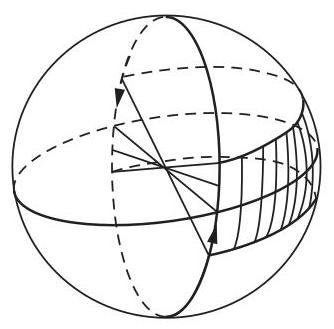
\includegraphics[max width=0.3\textwidth]{images/bo_d4b9jf3ef24c73e0334g_452_201_1788_334_329_0.jpg}
\end{center}
\hspace*{3em} 

图 5.52.射影平面包含一个莫比乌斯带.

通过类似的论证，可以证明示例 2 中的克莱因瓶 \(K\) 也是不可定向的.一般来说，每当一个正则曲面 \(S \subset  {R}^{3}\) 相对于 \({R}^{3}\) 的原点对称时，识别对称点就会产生一个不可定向的抽象曲面.

可以证明， \({R}^{3}\) 中的紧致正则曲面是可定向的(参见附注 2，第 2-7 节).因此， \({P}^{2}\) 和 \(K\) 不能嵌入到 \({R}^{3}\) 中，同样的情况也发生在上面生成的紧致不可定向曲面上.因此，我们在 \({R}^{3}\) 中遗漏了相当数量的曲面.

然而， \({P}^{2}\) 和 \(K\) 可以嵌入到 \({R}^{4}\) 中.对于克莱因瓶 \(K\) ，考虑由以下方式给出的映射 \(G : {R}^{2} \rightarrow  {R}^{4}\) :

\[
G\left( {u,v}\right)  = \left( {\left( {r\cos v + a}\right) \cos u,\left( {r\cos v + a}\right) \sin u,}\right.
\]

\[
\left. {r\sin v\cos \frac{u}{2},r\sin v\sin \frac{u}{2}}\right) \text{ . }
\]

注意到 \(G\left( {u,v}\right)  = G\left( {u + {2m\pi },{2n\pi } - v}\right)\) ，其中 \(m\) 和 \(n\) 是整数.因此， \(G\) 诱导了一个映射 \(\psi\) ，该映射作用于通过正方形得到的空间

\[
\left\lbrack  {0,{2\pi }}\right\rbrack   \times  \left\lbrack  {0,{2\pi }}\right\rbrack   \subset  {R}^{2}
\]

通过首先将其一条边反射到该边的中心，然后识别相对的边(参见图 5-53).这可以看作是克莱因瓶，如示例 2 中所定义，通过丢弃一个环面中一对对点被识别的开放一半，并观察这两种过程都导致相同的曲面(图 5-53).

\begin{center}
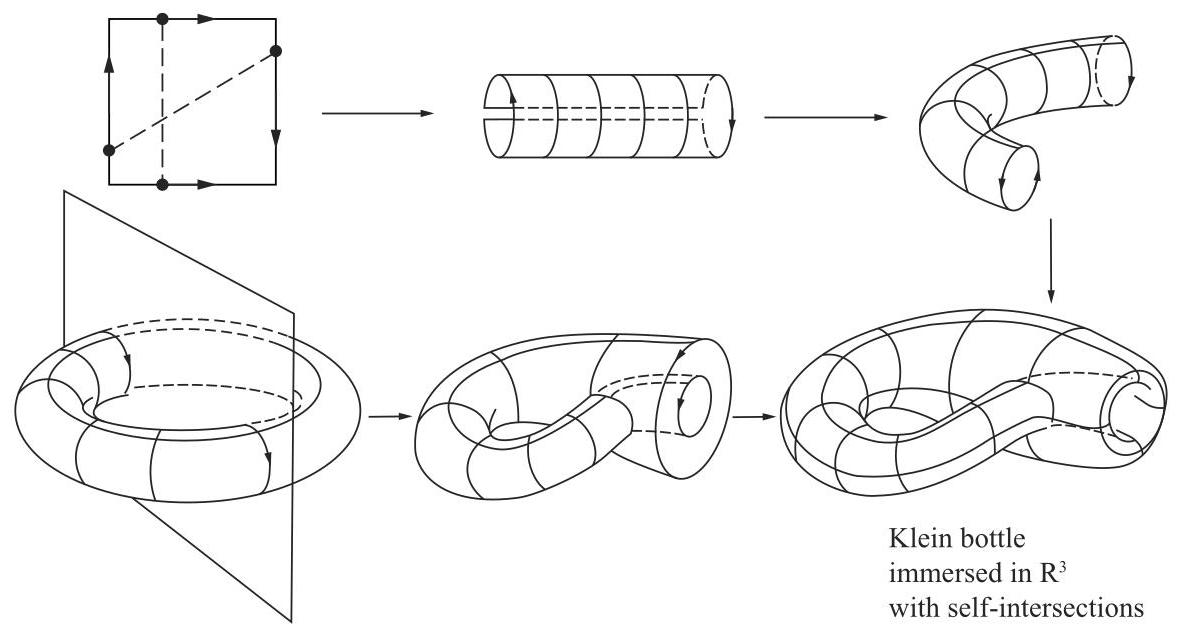
\includegraphics[max width=1.0\textwidth]{images/bo_d4b9jf3ef24c73e0334g_453_182_1392_1179_633_0.jpg}
\end{center}
\hspace*{3em} 

图 5-53

因此， \(\psi\) 是从 \(K\) 到 \({R}^{4}\) 的一个映射.进一步观察到

\[
G\left( {u + {4m\pi },v + {2m\pi }}\right)  = G\left( {u,v}\right) .
\]

由此可知 \(G = \psi  \circ  {\pi }_{1} \circ  \pi\) ，其中 \(\pi  : {R}^{2} \rightarrow  T\) 本质上是圆环 \(T\) 上的自然投影(参见示例 4)，而 \({\pi }_{1} : T \rightarrow  K\) 对应于识别 \(T\) 中的“一对对”点.根据 \(T\) 和 \(K,\pi\) 以及 \({\pi }_{1}\) 的可微结构的定义，它们是局部微分同胚.因此， \(\psi  : K \rightarrow  {R}^{4}\) 是可微的，并且 \({d\psi }\) 的秩与 \({dG}\) 的秩相同.后者很容易计算为 2；因此， \(\psi\) 是一个浸入.由于 \(K\) 是紧致的且 \(\psi\) 是一一对应的， \({\psi }^{-1}\) 很容易看出是 \(\varphi \left( K\right)\) 上的连续映射.因此， \(\psi\) 是一个嵌入，正如我们所期望的.

对于射影平面 \({P}^{2}\) ，考虑由以下方式给出的映射 \(F : {R}^{3} \rightarrow  {R}^{4}\) :

\[
F\left( {x,y,z}\right)  = \left( {{x}^{2} - {y}^{2},{xy},{xz},{yz}}\right) .
\]

设 \({S}^{2} \subset  {R}^{3}\) 为以 \({R}^{3}\) 的原点为中心的单位球面.显然，限制 \(\varphi  = F/{S}^{2}\) 使得 \(\varphi \left( p\right)  = \varphi \left( {-p}\right)\) .因此， \(\varphi\) 诱导了一个映射

\[
\widetilde{\varphi } : {P}^{2} \rightarrow  {R}^{4}\text{ by }\widetilde{\varphi }\left( {\{ p, - p\} }\right)  = \varphi \left( p\right) .
\]

为了看出 \(\varphi\) (因此， \(\widetilde{\varphi }\) )是一个浸入，考虑由 \(\mathbf{x}\left( {x,y}\right)  = \left( {x,y, + \sqrt{1 - {x}^{2} - {y}^{2}}}\right.\) 给出的 \({S}^{2}\) 的参数化 \(\mathbf{x}\) ，其中 \({x}^{2} + {y}^{2} \leq  1\) .那么

\[
\varphi  \circ  \mathbf{x}\left( {x,y}\right)  = \left( {{x}^{2} - {y}^{2},{xy},{xD},{yD}}\right) ,\;D = \sqrt{1 - {x}^{2} - {y}^{2}}.
\]

很容易验证 \(d\left( {\varphi  \circ  \mathbf{x}}\right)\) 的矩阵秩为 2.因此， \(\widetilde{\varphi }\) 是一个浸入.

为了看出 \(\widetilde{\varphi }\) 是单射，令

\[
{x}^{2} - {y}^{2} = a,\;{xy} = b,\;{xz} = c,\;{yz} = d. \tag{2}
\]

只需证明，在条件 \({x}^{2} + {y}^{2} + {z}^{2} = 1\) 下，上述方程只有两个解，形式为 \(\left( {x,y,z}\right)\) 和 \(\left( {-x, - y, - z}\right)\) .事实上，我们可以写出

\[
{x}^{2}d = {bc},\;{y}^{2}c = {bd},
\]

\[
{z}^{2}b = {cd},\;{x}^{2} - {y}^{2} = a, \tag{3}
\]

\[
{x}^{2} + {y}^{2} + {z}^{2} = 1
\]

其中前三个方程来自 (2) 的最后三个方程.

现在，如果数字 \(b,c,d\) 中有一个不为零，则 (3) 中的方程将给出 \({x}^{2},{y}^{2}\) 和 \({z}^{2}\) ，而 (2) 中的方程将确定两个坐标的符号，一旦给定其余一个坐标的符号.如果 \(b = c = d = 0\) ，则 (2) 中的方程和 (3) 的最后一个方程表明恰好有两个坐标为零，其余一个为 \(\pm  1\) .在任何情况下，解都具有要求的形式，并且 \(\widetilde{\varphi }\) 是单射.

通过紧致性， \(\varphi\) 是一个嵌入，这就完成了示例.

回顾抽象曲面的定义，我们看到数字 2 没有起到本质作用.因此，我们可以将该定义扩展到任意 \(n\) ，并且正如我们即将看到的，这可能是有用的.

定义 1a.维度为 \(N\) 的 \(A\) 可微流形是一个集合 \(\mathrm{M}\) ，以及一组从开集 \({\mathrm{U}}_{\alpha } \subset  {\mathbb{R}}^{N}\) 到 \(\mathrm{M}\) 的单射映射 \({\mathbf{x}}_{\alpha } : {\mathrm{U}}_{\alpha } \rightarrow  \mathrm{M}\) ，使得

1. \(\mathop{\bigcup }\limits_{\alpha }{\mathbf{x}}_{\alpha }\left( {\mathrm{U}}_{\alpha }\right)  = \mathrm{M}\) .

2. 对于每一对 \(\alpha ,\beta\) 和 \({\mathbf{x}}_{\alpha }\left( {\mathrm{U}}_{\alpha }\right)  \cap  {\mathbf{x}}_{\beta }\left( {\mathrm{U}}_{\beta }\right)  = W \neq  \phi\) ，我们有 \({\mathbf{x}}_{\alpha }^{-1}\left( \mathrm{\;W}\right) ,{\mathbf{x}}_{\beta }^{-1}\left( \mathrm{\;W}\right)\) 是 \({\mathbb{R}}^{N}\) 中的开集，并且 \({\mathbf{x}}_{\beta }^{-1} \circ  {\mathbf{x}}_{\alpha },{\mathbf{x}}_{\alpha }^{-1} \circ  {\mathbf{x}}_{\beta }\) 是可微映射.

3. 族 \(\left\{  {{\mathrm{U}}_{\alpha },{\mathbf{x}}_{\alpha }}\right\}\) 相对于条件 1 和 2 是极大的.

满足条件 1 和 2 的族 \(\left\{  {{U}_{\alpha },{\mathbf{x}}_{\alpha }}\right\}\) 称为 \(M\) 上的可微结构.给定 \(M\) 上的可微结构，我们可以通过添加所有可能的参数化来轻松地将其完成为一个极大的结构，这些参数化与族 \(\left\{  {{U}_{\alpha },{\mathbf{x}}_{\alpha }}\right\}\) 的某个参数化一起满足条件 2.因此，我们可能略微滥用语言说，可微流形是带有可微结构的集合.

注. \(M\) 中的开集族可以通过以下条件定义:如果对于每一个 \(\alpha ,{\mathbf{x}}_{\alpha }^{-1}\left( {V \cap  {\mathbf{x}}_{\alpha }\left( {U}_{\alpha }\right) }\right)\) ， \(V \subset  M\) 是 \({R}^{n}\) 中的一个开集，则 \(V \subset  M\) 是一个开集.具有点集拓扑知识的读者会注意到，这样的族在 \(M\) 上定义了一个自然拓扑.在此拓扑下，映射 \({\mathbf{x}}_{\alpha }\) 是连续的，集合 \({\mathbf{x}}_{\alpha }\left( {U}_{\alpha }\right)\) 在 \(M\) 中是开集.在关于流形的某些更深入的定理中，有必要对 \(M\) 的自然拓扑施加一些条件.

可微映射和切向量的定义逐字地推广到可微流形.当然，切空间现在是一个 \(n\) 维向量空间.微分和可定向性的定义也直接扩展到当前情况.

在下面的例子中，我们将展示二维流形上的问题如何自然地引出对高维流形的考虑.

例 6. (切丛).设 \(S\) 为一个抽象曲面，设 \(T\left( S\right)  = \left\{  {\left( {p,w}\right) ,p \in  S,w \in  {T}_{p}\left( S\right) }\right\}\) .我们将证明集合 \(T\left( S\right)\) 可以赋予一个可微结构(维度为 4)，称为 \(S\) 的切丛.

设 \(\left\{  {{U}_{\alpha },{\mathbf{x}}_{\alpha }}\right\}\) 为 \(S\) 的一个可微结构.我们将用 \(\left( {{u}_{\alpha },{v}_{\alpha }}\right)\) 表示 \({U}_{\alpha }\) 的坐标，用 \(\left\{  {\partial /\partial {u}_{\alpha },\partial /\partial {v}_{\alpha }}\right\}\) 表示 \({\mathbf{x}}_{\alpha }\left( {U}_{\alpha }\right)\) 的切平面中的相关基.对于每个 \(\alpha\) ，定义一个映射 \({\mathbf{y}}_{\alpha } : {U}_{\alpha } \times  {R}^{2} \rightarrow  T\left( S\right)\) 为

\[
{\mathbf{y}}_{\alpha }\left( {{u}_{\alpha },{v}_{\alpha },x,y}\right)  = \left( {{\mathbf{x}}_{\alpha }\left( {{u}_{\alpha },{v}_{\alpha }}\right) ,x\frac{\partial }{\partial {u}_{\alpha }} + y\frac{\partial }{\partial {v}_{\alpha }}}\right) ,\;\left( {x,y}\right)  \in  {R}^{2}.
\]

几何上，这意味着我们将取一个点 \(\left( {p,w}\right)  \in  T\left( S\right)\) 的坐标为 \(p\) 的坐标 \({u}_{\alpha },{v}_{\alpha }\) 加上 \(w\) 在基 \(\left\{  {\partial /\partial {u}_{\alpha },\partial /\partial {v}_{\alpha }}\right\}\) 中的坐标.

我们将证明 \(\left\{  {{U}_{\alpha } \times  {R}^{2},{\mathbf{y}}_{\alpha }}\right\}\) 是 \(T\left( S\right)\) 的一个可微结构.因为 \(\mathop{\bigcup }\limits_{\alpha }{\mathbf{x}}_{\alpha }\left( {U}_{\alpha }\right)  = S\) 和 \({\left( d{\mathbf{x}}_{\alpha }\right) }_{q}\left( {R}^{2}\right)  = {T}_{{\mathbf{x}}_{\alpha }\left( q\right) }\left( S\right) ,q \in  {U}_{\alpha }\) ，我们有

\[
\mathop{\bigcup }\limits_{\alpha }{\mathbf{y}}_{\alpha }\left( {{U}_{\alpha } \times  {R}^{2}}\right)  = T\left( S\right)
\]

并且这满足定义 1a 的条件 1.现在设

\[
\left( {p,w}\right)  \in  {\mathbf{y}}_{\alpha }\left( {{U}_{\alpha } \times  {R}^{2}}\right)  \cap  {\mathbf{y}}_{\beta }\left( {{U}_{\beta } \times  {R}^{2}}\right) .
\]

那么

\[
\left( {p,w}\right)  = \left( {{\mathbf{x}}_{\alpha }\left( {q}_{\alpha }\right) ,d{\mathbf{x}}_{\alpha }\left( {w}_{\alpha }\right) }\right)  = \left( {{\mathbf{y}}_{\beta }\left( {q}_{\beta }\right) ,d{\mathbf{x}}_{\beta }\left( {w}_{\beta }\right) }\right) ,
\]

其中 \({q}_{\alpha } \in  {U}_{\alpha },{q}_{\beta } \in  {U}_{\beta },{w}_{\alpha },{w}_{\beta } \in  {R}^{2}\) .因此，

\[
{\mathbf{y}}_{\beta }^{-1} \circ  {\mathbf{y}}_{\alpha }\left( {{q}_{\alpha },{w}_{\alpha }}\right)  = {\mathbf{y}}_{\beta }^{-1}\left( {{\mathbf{x}}_{\alpha }\left( {q}_{\alpha }\right) ,d{\mathbf{x}}_{\alpha }\left( {w}_{\alpha }\right) }\right)
\]

\[
= \left( {\left( {{\mathbf{x}}_{\beta }^{-1} \circ  {\mathbf{x}}_{\alpha }}\right) \left( {q}_{\alpha }\right) ,d\left( {{\mathbf{x}}_{\beta }^{-1} \circ  {\mathbf{x}}_{\alpha }}\right) \left( {w}_{\alpha }\right) }\right) .
\]

因为 \({\mathbf{x}}_{\beta }^{-1} \circ  {\mathbf{x}}_{\alpha }\) 是可微的，所以 \(d\left( {{\mathbf{x}}_{\beta }^{-1} \circ  {\mathbf{x}}_{\alpha }}\right)\) 也是可微的.由此可知 \({\mathbf{y}}_{\beta }^{-1} \circ  {\mathbf{y}}_{\alpha }\) 是可微的，并且这满足定义 1a 的条件 2.

当处理 \(S\) 上的二阶微分方程时， \(S\) 的切丛是自然的工作空间.例如，几何曲面 \(S\) 上的测地线方程可以在一个坐标邻域中写成(参见第 4-7 节)

\[
{u}^{\prime \prime } = {f}_{1}\left( {u,v,{u}^{\prime },{v}^{\prime }}\right) ,
\]

\[
{v}^{\prime \prime } = {f}_{2}\left( {u,v,{u}^{\prime },{v}^{\prime }}\right) .
\]

引入新变量 \(x = {u}^{\prime },y = {v}^{\prime }\) 以将上述方程化简为一阶系统

\[
{x}^{\prime } = {f}_{1}\left( {u,v,x,y}\right) ,
\]

(4)
\[
{y}^{\prime } = {f}_{2}\left( {u,v,x,y}\right) ,
\]

\[
{u}^{\prime } = {f}_{3}\left( {u,v,x,y}\right) ,
\]

\[
{v}^{\prime } = {f}_{4}\left( {u,v,x,y}\right)
\]

可被解释为考虑切丛 \(T\left( S\right)\) ，其坐标为 \(\left( {u,v,x,y}\right)\) ，并将测地线视为由 \(T\left( S\right)\) 中局部由 (4) 给出的向量场的轨迹.可以证明，这样的向量场在整个 \(T\left( S\right)\) 中是良定义的；也就是说，在两个坐标邻域的交集中，由 (4) 给出的向量场是相同的.这个场(或者更确切地说，它的轨迹)被称为 \(T\left( S\right)\) 上的测地流.在研究 \(S\) 上的测地线的全局性质时，这是一个非常自然的工具.

回顾第 4-7 节，我们会注意到我们已经以一种伪装的形式使用了流形 \(T\left( S\right)\) .由于我们只对局部性质感兴趣，我们可以使用一个坐标邻域(本质上是 \({R}^{4}\) 的一个开集).然而，即使是这种局部工作，当考虑切丛的概念时，也会变得更加简洁.

当然，我们也可以定义任意 \(n\) 维流形的切丛.除了记号外，细节是相同的，将留作练习.

我们也可以将几何曲面的概念推广到任意维度.

定义 5a.黎曼流形是一个 n 维可微流形 \(\mathrm{M}\) ，以及对每个 \(\mathrm{p} \in  \mathrm{M}\) 的选择，一个内积 \(\langle\) ， \({\rangle }_{p}\) 在 \({\mathrm{T}}_{\mathrm{p}}\left( \mathrm{M}\right)\) 中，它随 \(\mathrm{p}\) 可微地变化，具体如下.对于某个(因此，所有)参数化 \({\mathbf{x}}_{\alpha } : {\mathrm{U}}_{\alpha } \rightarrow  \mathrm{M}\) ，其中 \(\mathrm{p} \in  {\mathbf{x}}_{\alpha }\left( {\mathrm{U}}_{\alpha }\right)\) ，函数

\[
{\mathrm{g}}_{\mathrm{{ij}}}\left( {{\mathrm{u}}_{1}\ldots ,{\mathrm{u}}_{N}}\right)  = \left\langle  {\frac{\partial }{\partial {\mathrm{u}}_{\mathrm{i}}},\frac{\partial }{\partial {\mathrm{u}}_{\mathrm{j}}}}\right\rangle  ,\;\mathrm{i},\mathrm{j} = 1,\ldots ,N,
\]

在 \({\mathbf{x}}_{\alpha }^{-1}\left( \mathrm{p}\right)\) 处可微；这里 \(\left( {{\mathrm{u}}_{1},\ldots ,{\mathrm{u}}_{N}}\right)\) 是 \({\mathrm{U}}_{\alpha } \subset  {\mathbb{R}}^{N}\) 的坐标.

可微族 \(\left\{  {\langle \;{\rangle }_{p},p \in  M}\right\}\) 被称为 \(M\) 的黎曼结构(或黎曼度量).

请注意，在曲面的情况下，我们使用了传统的记号 \({g}_{11} = E,{g}_{12} = {g}_{21} = F,{g}_{22} = G.\) .

将内蕴几何的概念推广到黎曼流形不像推广到可微流形那样直接.

首先，我们必须为黎曼流形定义一个协变导数的概念.为此，设 \(\mathbf{x} : U \rightarrow  M\) 为一个具有坐标 \(\left( {{u}_{1},\ldots ,{u}_{n}}\right)\) 的参数化，并设 \({\mathbf{x}}_{i} = \partial /\partial {u}_{i}\) .因此， \({g}_{ij} = \left\langle  {{\mathbf{x}}_{i},{\mathbf{x}}_{j}}\right\rangle\) .

我们想定义一个向量场 \(v\) 相对于向量场 \(w\) 的协变导数 \({D}_{w}v\) .我们希望 \({D}_{w}v\) 具有我们习惯的并且过去被证明是有效的性质.首先，它应该具有旧的协变导数的分配性质.因此，如果 \(u,v\) ， \(w\) 是 \(M\) 上的向量场，而 \(f,g\) 是 \(M\) 上的可微函数，我们希望

\[
{D}_{{fu} + {gw}}\left( v\right)  = f{D}_{u}v + g{D}_{w}v, \tag{5}
\]

\[
{D}_{u}\left( {{fv} + {gw}}\right)  = f{D}_{u}v + \frac{\partial f}{\partial u}v + g{D}_{u}w + \frac{\partial g}{\partial u}w, \tag{6}
\]

其中 \(\partial f/\partial u\) 例如是一个函数，其在 \(p \in  M\) 处的值是 \(f\) 在曲线 \(\alpha  : \left( {-\epsilon ,\epsilon }\right)  \rightarrow  M,\alpha \left( 0\right)  = p\) 上的限制的导数 \({\left( f \circ  \alpha \right) }^{\prime }\left( 0\right)\) ， \({\alpha }^{\prime }\left( 0\right)  = u.\)

方程 (5) 和 (6) 表明，协变导数 \(D\) 一旦在其基向量上的值确定，就完全确定了.

\[
{D}_{{\mathbf{x}}_{i}}{\mathbf{x}}_{j} = \mathop{\sum }\limits_{{k = 1}}^{n}{\Gamma }_{ij}^{k}{\mathbf{x}}_{k},\;i,j,k = 1,\ldots ,n,
\]

其中系数 \({\Gamma }_{ij}^{k}\) 是待定的弧函数.

其次，我们希望 \({\Gamma }_{ij}^{k}\) 在 \(i\) 和 \(j\left( {{\Gamma }_{ij}^{k} = {\Gamma }_{ji}^{k}}\right)\) 上是对称的；即，

\[
{D}_{{\mathbf{x}}_{i}}{\mathbf{x}}_{j} = {D}_{{\mathbf{x}}_{j}}{\mathbf{x}}_{i}\;\text{ for all }i,j. \tag{7}
\]

第三，我们希望乘积法则成立；即，

\[
\frac{\partial }{\partial {u}_{k}}\left\langle  {{\mathbf{x}}_{i},{\mathbf{x}}_{j}}\right\rangle   = \left\langle  {{\mathbf{D}}_{{\mathbf{x}}_{k}}{\mathbf{x}}_{i},{\mathbf{x}}_{j}}\right\rangle   + \left\langle  {{\mathbf{x}}_{i},{\mathbf{D}}_{{\mathbf{x}}_{k}}{\mathbf{x}}_{j}}\right\rangle  . \tag{8}
\]

从方程 (7) 和 (8) 可知，

\[
\frac{\partial }{\partial {u}_{k}}\left\langle  {{\mathbf{x}}_{i}{\mathbf{x}}_{j}}\right\rangle   + \frac{\partial }{\partial {u}_{i}}\left\langle  {{\mathbf{x}}_{j},{\mathbf{x}}_{k}}\right\rangle   - \frac{\partial }{\partial {u}_{j}}\left\langle  {{\mathbf{x}}_{k},{\mathbf{x}}_{i}}\right\rangle   = 2\left\langle  {{\mathbf{D}}_{{\mathbf{x}}_{i}}{\mathbf{x}}_{k},{\mathbf{x}}_{j}}\right\rangle  ,
\]

或者等价地，

\[
\frac{\partial }{\partial {u}_{k}}{g}_{ij} + \frac{\partial }{\partial {u}_{i}}{g}_{jk} - \frac{\partial }{\partial {u}_{j}}{g}_{ki} = 2\mathop{\sum }\limits_{i}{\Gamma }_{ik}^{i}{g}_{ij}.
\]

由于 \(\det \left( {g}_{ij}\right)  \neq  0\) ，我们可以解出最后一个方程组，得到 \({\Gamma }_{ij}^{k}\) 作为黎曼度量 \({g}_{ij}\) 及其导数的函数(读者应将上述方程组与第 4-3 节的方程组 (2) 进行比较).如果我们把 \({g}_{ij}\) 看作一个矩阵，并写出其逆矩阵为 \({g}^{ij}\) ，则上述方程组的解为

\[
{\Gamma }_{ij}^{k} = \frac{1}{2}\mathop{\sum }\limits_{l}{g}^{kl}\left( {\frac{\partial {g}_{il}}{\partial {u}_{j}} + \frac{\partial {g}_{jl}}{\partial {u}_{i}} - \frac{\partial {g}_{ij}}{\partial {u}_{l}}}\right) .
\]

因此，给定 M 的一个黎曼结构，存在一个唯一的协变导数(也称为给定黎曼结构的 Levi-Civita 连接)，它满足方程 (5)-(8).

从协变导数出发，我们可以定义平行移动、测地线、测地曲率、指数映射、完备性等.

这些定义与我们之前给出的定义完全相同.然而，曲率的概念需要进一步阐述.以下由黎曼提出的概念可能是黎曼几何中高斯曲率的最佳类比.

设 \(p \in  M\) ，令 \(\sigma  \subset  {T}_{p}\left( M\right)\) 为切空间 \({T}_{p}\left( M\right)\) 的一个二维子空间.考虑所有从 \(p\) 开始且切线方向为 \(\sigma\) 的 \(M\) 的测地线.由于指数映射在 \({T}_{p}\left( M\right)\) 的原点处是局部微分同胚，可以证明这些测地线的小段构成了包含 \(p.S\) 的一个抽象曲面 \(S\) ，该曲面具有由 \(M\) 的黎曼结构诱导的自然几何结构.曲面 \(S\) 在 \(p\) 处的曲率称为 \(M\) 在 \(p\) 处沿 \(\sigma\) 的截面曲率 \(K\left( {p,\sigma }\right)\) .

有可能用 Levi-Civita 连接来形式化截面曲率，但这过于技术性，在此不作描述.我们只提及本章中的大部分定理都可以作为黎曼几何中的自然问题来提出.其中一些定理只需稍作修改或无需修改即可证明.(Hopf-Rinow 定理、Bonnet 定理、第一个 Hadamard 定理和 Jacobi 定理都属于此类.)然而，另一些定理需要进一步的假设才能成立(例如，第二个 Hadamard 定理)，并为进一步发展提供了基础.

对上述思想的全面发展将把我们引入黎曼几何的领域.我们必须在此停止，并将读者引向书末的参考文献.

\exerciseline

1. 在射影平面 \({P}^{2}\) 上引入一个度量(参见示例 1)，使得自然投影 \(\pi  : {S}^{2} \rightarrow  {P}^{2}\) 是一个局部等距映射.这样的度量的(高斯)曲率是多少？

2. (无限莫比乌斯带.)令

\[
C = \left\{  {\left( {x,y,z}\right)  \in  {R}^{3};{x}^{2} + {y}^{2} = 1}\right\}
\]

为一个圆柱体，令 \(A : C \rightarrow  C\) 为映射(对径映射) \(A\left( {x,y,z}\right)  = \; \left( {-x, - y, - z}\right)\) .令 \(M\) 为 \(C\) 关于等价关系 \(p \sim  A\left( p\right)\) 的商空间，令 \(\pi  : C \rightarrow  M\) 为映射 \(\pi \left( p\right)  = \{ p,A\left( p\right) \} ,p \in  C\) .

a. 证明可以赋予 \(M\) 一个可微结构，使得 \(\pi\) 是一个局部微分同胚(此时 \(M\) 称为无限莫比乌斯带).

b. 证明 \(M\) 是不可定向的.

c. 在 \(M\) 上引入一个黎曼度量，使得 \(\pi\) 是一个局部等距.这样的度量的曲率是多少？

3. a. 证明从球面到射影平面的投影 \(\pi  : {S}^{2} \rightarrow  {P}^{2}\) 具有以下性质:(1) \(\pi\) 是连续的且 \(\pi \left( {S}^{2}\right)  = {P}^{2}\) ；(2) 每个点 \(p \in  {P}^{2}\) 都有一个邻域 \(U\) ，使得 \({\pi }^{-1}\left( U\right)  = {V}_{1} \cup  {V}_{2}\) ，其中 \({V}_{1}\) 和 \({V}_{2}\) 是 \({S}^{2}\) 中不相交的开子集，并且 \(\pi\) 在每个 \({V}_{i},i = 1,2\) 上的限制是到 \(U\) 的一个同胚.因此， \(\pi\) 在形式上满足覆盖映射(见第 5-6 节，定义 1)的条件，具有两张片.因此，我们称 \({S}^{2}\) 是 \({P}^{2}\) 的一个定向双覆盖.

b. 证明在此意义下，环面 \(T\) 是克莱因瓶 \(K\) 的一个定向双覆盖(参见例 2)，并且圆柱体是无限莫比乌斯带(参见练习 2)的一个定向双覆盖.

4. (定向双覆盖).本练习给出了一个不可定向曲面的定向双覆盖的通用构造.令 \(S\) 为一个抽象的、连通的、不可定向曲面.对于每个 \(p \in  S\) ，考虑所有 \({T}_{p}\left( S\right)\) 的基的集合 \(B\) ，并将两个基称为等价的，如果它们可以通过一个具有正行列式的矩阵相关联.这显然是一个等价关系，并将 \(B\) 分为两个不相交的集合(参见第 1-4 节).令 \({\mathfrak{O}}_{p}\) 为 \(B\) 关于此等价关系的商空间. \({\mathfrak{O}}_{p}\) 有两个元素，每个元素 \({O}_{p} \in  {\mathfrak{O}}_{p}\) 都是 \({T}_{p}\left( S\right)\) 的一个定向(参见第 1-4 节).令 \(\widetilde{S}\) 为集合

\[
\widetilde{S} = \left\{  {\left( {p,{O}_{p}}\right) ;p \in  S;{O}_{p} \in  {\mathfrak{O}}_{p}}\right\}  .
\]

为了赋予 \(\widetilde{S}\) 一个可微结构，令 \(\left\{  {{U}_{\alpha },{\mathbf{x}}_{\alpha }}\right\}\) 为 \(S\) 的最大可微结构，并定义 \({\widetilde{\mathbf{x}}}_{\alpha } : {U}_{\alpha } \rightarrow  \widetilde{S}\) 为

\[
{\widetilde{\mathbf{x}}}_{\alpha }\left( {{u}_{\alpha },{v}_{\alpha }}\right)  = \left( {{\mathbf{x}}_{\alpha }\left( {{u}_{\alpha },{v}_{\alpha }}\right) ,\left\lbrack  {\frac{\partial }{\partial {u}_{\alpha }},\frac{\partial }{\partial {v}_{\alpha }}}\right\rbrack  }\right) ,
\]

其中 \(\left( {{u}_{\alpha },{v}_{\alpha }}\right)  \in  {U}_{\alpha }\) 和 \(\left\lbrack  {\partial /\partial {u}_{\alpha },\partial /\partial {v}_{\alpha }}\right\rbrack\) 表示由基 \(\left\{  {\partial /\partial {u}_{\alpha },\partial /\partial {v}_{\alpha }}\right\}\) 确定的 \({\mathfrak{O}}_{p}\) 的元素.证明

a. \(\left\{  {{U}_{\alpha },{\widetilde{\mathbf{x}}}_{\alpha }}\right\}\) 是 \(\widetilde{S}\) 上的一个可微结构，并且具有这种可微结构的 \(\widetilde{S}\) 是一个可定向曲面.

b. 映射 \(\pi  : \widetilde{S} \rightarrow  S\) 由 \(\pi \left( {p,{O}_{p}}\right)  = p\) 给出，是一个可微满射.此外，每个点 \(p \in  S\) 都有一个邻域 \(U\) ，使得 \({\pi }^{-1}\left( U\right)  = {V}_{1} \cup  {V}_{2}\) ，其中 \({V}_{1}\) 和 \({V}_{2}\) 是 \(\widetilde{S}\) 的不相交开子集，并且 \(\pi\) 限制在每个 \({V}_{i},i = 1,2\) 上，是一个到 \(U\) 的微分同胚.因此， \(\widetilde{S}\) 被称为 \(S\) 的一个可定向双覆盖.

5. 将高斯-博内定理(参见第 4-5 节)推广到可定向几何曲面，并应用它来证明以下事实:

a. 在一个同胚于环面的抽象曲面 \(T\) 上，不存在一个黎曼度量，使得其在 \(T\) 的所有点的曲率都为正(或为负).

b. 令 \(T\) 和 \({S}^{2}\) 分别为同胚于环面和球面的抽象曲面，令 \(\varphi  : T \rightarrow  {S}^{2}\) 为一个可微映射.则 \(\varphi\) 至少有一个临界点，即一个点 \(p \in  T\) ，使得 \(\det \left( {d{\varphi }_{p}}\right)  = 0.\)

6. 考虑上半平面 \({R}_{ + }^{2}\) (参见例 3)，其度量为

\[
E\left( {x,y}\right)  = 1,\;F\left( {x,y}\right)  = 0,\;G\left( {x,y}\right)  = \frac{1}{y},\;\left( {x,y}\right)  \in  {R}_{ + }^{2}.
\]

证明当接近 \({R}_{ + }^{2}\) 的边界时，向量的长度任意增大，而垂直线段的长度

\[
x = 0,\;0 < \epsilon  \leq  y \leq  1,
\]

当 \(\epsilon  \rightarrow  0\) 时趋近于 2.由此得出该度量不是完备的.

*7. 证明庞加莱上半平面(参见例 3)是一个完备的几何曲面.由此得出双曲平面是完备的.

8. 找到庞加莱上半平面(参见例 3)的测地线的另一种方法是使用相应变分问题的欧拉-拉格朗日方程(参见第 5-4 节练习 4).由于我们知道垂直线是测地线，我们可以将自己限制在形式为 \(y = y\left( x\right)\) 的测地线上.因此，我们必须寻找积分 \(\left( {F = 0}\right)\) 的临界点

\[
\int \sqrt{E + G{\left( {y}^{\prime }\right) }^{2}}{dx} = \int \sqrt{\frac{1 + {\left( {y}^{\prime }\right) }^{2}}{y}}{dx},
\]

因为 \(E = G = 1/{y}^{2}\) .使用第 5-4 节练习 4 来证明该变分问题的解是一族形式为

\[
{\left( x + {k}_{1}\right) }^{2} + {y}^{2} = {k}_{2}^{2},\;{k}_{1},{k}_{2} = \text{ const. }
\]

9. 设 \(\widetilde{S}\) 和 \(S\) 为连通的几何曲面，设 \(\pi  : \widetilde{S} \rightarrow  S\) 为一个具有以下性质的满射可微映射:对于每个 \(p \in  S\) ，存在 \(p\) 的一个邻域 \(U\) ，使得 \({\pi }^{-1}\left( U\right)  = \mathop{\bigcup }\limits_{\alpha }{V}_{\alpha }\) ，其中 \({V}_{\alpha }\) 是 \(\widetilde{S}\) 的开不相交子集，并且 \(\pi\) 在每个 \({V}_{\alpha }\) 上的限制是到 \(U\) 的等距映射(因此， \(\pi\) 本质上是一个覆盖映射和局部等距映射).

a. 证明 \(S\) 是完备的当且仅当 \(\widetilde{S}\) 是完备的.

b. 在习题 2 c 部分介绍的无限莫比乌斯带上的度量是完备度量吗？

10. (Kazdan-Wamer 的结果.)

a. 令 \({R}^{2}\) 上的度量由下式给出

\[
E\left( {x,y}\right)  = 1,\;F\left( {x,y}\right)  = 0,\;G\left( {x,y}\right)  > 0,\;\left( {x,y}\right)  \in  {R}^{2}.
\]

证明该度量的曲率由下式给出

\[
\frac{{\partial }^{2}\left( \sqrt{G}\right) }{\partial {x}^{2}} + K\left( {x,y}\right) \sqrt{G} = 0.
\]
 (*)

b. 反之，给定 \({R}^{2}\) 上的一个函数 \(K\left( {x,y}\right)\) ，将 \(y\) 看作参数，令 \(\sqrt{G}\) 为 \(\left( *\right)\) 在初始条件下的解

\[
\sqrt{G}\left( {{x}_{0},y}\right)  = 1,\;\frac{\partial \sqrt{G}}{\partial x}\left( {{x}_{0},y}\right)  = 0.
\]

证明 \(G\) 在 \(\left( {{x}_{0},y}\right)\) 的邻域内是正的，因此在该邻域内定义了一个度量.这表明每个可微函数在局部上是某个(抽象)度量的曲率.

*c. 假设 \(K\left( {x,y}\right)  \leq  0\) 对所有 \(\left( {x,y}\right)  \in  {R}^{2}\) 都成立.证明第 \(\mathrm{b}\) 部分的解满足

\[
\sqrt{G\left( {x,y}\right) } \geq  \sqrt{G\left( {{x}_{0},y}\right) } = 1\text{ for all }x.
\]

因此， \(G\left( {x,y}\right)\) 在 \({R}^{2}\) 上定义了一个度量.也证明该度量是完备的.这表明 \({\mathbb{R}}^{2}\) 上的任何非正可微函数是 \({\mathbb{R}}^{2}\) 上某个完备度量的曲率.如果我们不坚持度量必须是完备的，那么对于 \({R}^{2}\) 上的任何可微函数 \(K\) ，该结果都是成立的.比较 J. Kazdan 和 F. Warner 的文章 "Curvature Functions for Open 2-Manifolds"，Ann. of Math. 99 (1974)，203-219，其中也证明了习题 2，第 5-4 节中给出的关于 \(K\) 的条件是度量完备的充要条件.

\section*{5-11. 希尔伯特定理}

希尔伯特定理可以表述如下.

定理. 一个具有常负曲率的完备几何曲面 S 不能等距地嵌入到 \({\mathbb{R}}^{3}\) 中.

注 1. 希尔伯特定理最早由 D. Hilbert 在 "Über Flächen von konstanter Gausscher Krümung"(关于常高斯曲率曲面)一文中首次提出，Trans. Amer. Math. Soc. 2 (1901)，87-99.不久之后，E. Holmgren 给出了一个不同的证明，"Sur les surfaces à courbure constante negative"(关于常负曲率曲面)，C. R. Acad. Sci. Paris 134 (1902)，740-743.我们将在此呈现的证明遵循希尔伯特最初的想法.局部部分与希尔伯特论文中的基本相同；然而，全局部分则有很大不同.我们要感谢 J. A. Scheinkman 帮助我们完成了这个证明.

我们将从一些观察开始.通过将内积乘以一个常数因子，我们可以假设曲率 \(K \equiv   - 1\) .此外，由于 \({\exp }_{p} : {T}_{p}\left( S\right)  \rightarrow  S\) 是一个局部微分同胚(第5-5节定理的推论)，它在 \({T}_{p}\left( S\right)\) 中诱导出一个内积.令 \({S}^{\prime }\) 表示具有此内积的几何曲面 \({T}_{p}\left( S\right)\) .如果 \(\psi  : S \rightarrow  {R}^{3}\) 是一个等距浸入，那么对于 \(\varphi  = \psi  \circ  {\exp }_{p} : {S}^{\prime } \rightarrow  {R}^{3}\) 也成立.因此，我们只需证明不存在一个平面 \({S}^{\prime }\) 到具有内积的几何曲面 \({T}_{p}\left( S\right)\) 的等距浸入 \(\varphi  : {S}^{\prime } - {R}^{3}\) ，使得 \(K \equiv   - 1\) .

引理 1. \({S}^{\prime }\) 的面积是无限的.

证明.我们将证明 \({S}^{\prime }\) 与双曲平面 \(H\) (全局)等距.由于后者的面积是(参见第5-10节例3)

\[
{\int }_{-\infty }^{+\infty }{\int }_{-\infty }^{+\infty }{e}^{u}{dudv} = \infty
\]

这将证明该引理.

令 \(p \in  H,{p}^{\prime } \in  {S}^{\prime }\) ，并在它们的切空间之间选择一个线性等距映射 \(\psi  : {T}_{p}\left( H\right)  \rightarrow  {T}_{{p}^{\prime }}\left( {S}^{\prime }\right)\) .通过 \(\varphi  = {\exp }_{p} \circ  \psi  \circ \; {\exp }_{p}^{-1}\) 定义映射 \(\varphi  : H \rightarrow  {S}^{\prime }\) .由于 \(H\) 的每个点都通过唯一的测地线与 \(p\) 相连，因此 \(\varphi\) 是良定义的.

我们现在使用 \(p\) 和 \({p}^{\prime }\) 周围的极坐标 \(\left( {p,\theta }\right)\) 和 \(\left( {{p}^{\prime },{\theta }^{\prime }}\right)\) ，要求 \(\varphi\) 将轴 \(\theta  = 0\) 映射到轴 \({\theta }^{\prime } = 0\) .根据第4-6节的结果， \(\varphi\) 保持第一基本形式；因此，它局部上是一个等距映射.通过使用Hadamard定理之后的注记，我们得出结论 \(\varphi\) 是一个覆盖映射.由于 \({S}^{\prime }\) 是单连通的， \(\varphi\) 是一个同胚，因此是一个(全局)等距映射.Q.E.D.

在本节的其余部分，我们将假设存在一个等距浸入 \(\varphi  : {S}^{\prime } \rightarrow  {R}^{3}\) ，其中 \({S}^{\prime }\) 是一个同胚于平面的几何曲面，并且具有 \(K \equiv   - 1\) .

为避免与 \(\varphi \left( {S}^{\prime }\right)\) 可能的自相交相关的困难，我们将使用 \({S}^{\prime }\) 并利用浸入 \(\varphi\) 在 \({S}^{\prime }\) 上诱导出 \(\varphi \left( {S}^{\prime }\right)  \subset  {R}^{3}\) 的局部外在几何.更精确地说，由于 \(\varphi\) 是一个浸入，对于每个 \(p \in  {S}^{\prime }\) 都存在 \(p\) 的一个邻域 \({V}^{\prime } \subset  {S}^{\prime }\) ，使得其限制 \(\varphi  \mid  {V}^{\prime } = \widetilde{\varphi }\) 是一个微分同胚.在每个 \(\widetilde{\varphi }\left( q\right)  \in  \widetilde{\varphi }\left( {V}^{\prime }\right)\) 处，例如，存在两个渐近方向.通过 \(\widetilde{\varphi }\) ，这些方向在 \(q \in  {S}^{\prime }\) 上诱导出两个方向，这两个方向将被称为 \({S}^{\prime }\) 在 \(q\) 处的渐近方向.这样，讨论 \({S}^{\prime }\) 上的渐近曲线就有了意义，并且同样的程序可以应用于 \(\varphi \left( {S}^{\prime }\right)\) 的任何其他局部实体.

我们现在回顾一下，参数化曲线的坐标曲线构成一个切比雪夫网，如果由它们形成的任何四边形的对边长度相等(参见练习 7，第 2-5 节).如果情况是这样，就可以重新参数化坐标邻域，使得 \(E = 1\) ， \(F = \cos \theta ,G = 1\) ，其中 \(\theta\) 是坐标曲线形成的夹角(第 2-5 节，练习 8).此外，在这种情况下， \(K =  - \left( {{\theta }_{uv}/\sin \theta }\right)\) (第 4-3 节，练习 5).

引理 2. 对于每个 \(\mathrm{p} \in  {S}^{\prime }\) 都存在一个参数化 \(\mathbf{x} : \mathrm{U} \subset  {\mathbb{R}}^{2} \rightarrow  {S}^{\prime }\) ， \(\mathrm{p} \in  \mathbf{x}\left( \mathrm{U}\right)\) ，使得 \(\mathbf{x}\) 的坐标曲线是 \(\mathbf{x}\left( \mathrm{U}\right)  = {\mathrm{V}}^{\prime }\) 的渐近曲线并构成一个切比雪夫网(我们将通过说 \({\mathrm{V}}^{\prime }\) 的渐近曲线构成一个切比雪夫网来表达这一点).

证明.由于 \(K < 0\) ， \(p\) 的一个邻域 \({V}^{\prime } \subset  {S}^{\prime }\) 可以通过 \(\mathbf{x}\left( {u,v}\right)\) 参数化，使得 \(\mathbf{x}\) 的坐标曲线是 \({V}^{\prime }\) 的渐近曲线.因此，如果 \(e,f\) 和 \(g\) 是 \({S}^{\prime }\) 在此参数化下的第二基本形式的系数，我们有 \(e = g = 0\) .请注意，我们使用了上述约定，即引用 \({S}^{\prime }\) 的第二基本形式而不是 \(\varphi \left( {S}^{\prime }\right)  \subset  {R}^{3}\) 的第二基本形式.

现在 \(\varphi \left( {V}^{\prime }\right)  \subset  {R}^{3}\) ，我们有

\[
{N}_{u} \land  {N}_{v} = K\left( {{\mathbf{x}}_{u} \land  {\mathbf{x}}_{v}}\right) ;
\]

因此，令 \(D = \sqrt{{EG} - {F}^{2}}\) ，

\[
{\left( N \land  {N}_{v}\right) }_{u} - {\left( N \land  {N}_{u}\right) }_{v} = 2\left( {{N}_{u} \land  {N}_{v}}\right)  = {2KDN}.
\]

此外，

\[
N \land  {N}_{u} = \frac{1}{D}\left\{  {\left( {{\mathbf{x}}_{u} \land  {\mathbf{x}}_{v}}\right)  \land  {N}_{u}}\right\}   = \frac{1}{D}\left\{  {\left\langle  {{\mathbf{x}}_{u},{N}_{u}}\right\rangle  {\mathbf{x}}_{v} - \left\langle  {{\mathbf{x}}_{v},{N}_{u}}\right\rangle  {\mathbf{x}}_{u}}\right\}
\]

\[
= \frac{1}{D}\left( {f{\mathbf{x}}_{u} - e{\mathbf{x}}_{v}}\right) ,
\]

类似地，

\[
N \land  {N}_{v} = \frac{1}{D}\left( {g{\mathbf{x}}_{u} - f{\mathbf{x}}_{v}}\right) .
\]

由于 \(K =  - 1 =  - \left( {{f}^{2}/{D}^{2}}\right)\) 和 \(e = g = 0\) ，我们得到

\[
N \land  {N}_{u} =  \pm  {\mathbf{x}}_{u},\;N \land  {N}_{v} =  \pm  {\mathbf{x}}_{v};
\]

因此

\[
2\mathrm{{KDN}} =  - 2\mathrm{{DN}} =  \pm  {\mathbf{x}}_{uv} \pm  {\mathbf{x}}_{vu} =  \pm  2{\mathbf{x}}_{uv}.
\]

由此可知 \({\mathbf{x}}_{uv}\) 平行于 \(N\) ；因此， \({E}_{v} = 2\left\langle  {{\mathbf{x}}_{uv},{\mathbf{x}}_{u}}\right\rangle   = 0\) 和 \({G}_{u} = \; 2\left\langle  {{\mathbf{x}}_{uv},{\mathbf{x}}_{v}}\right\rangle   = 0\) .但 \({E}_{v} = {G}_{u} = 0\) 暗示(第 2-5 节，练习 7)坐标曲线构成一个切比雪夫网.Q.E.D.

引理 3. 设 \({\mathrm{V}}^{\prime } \subset  {S}^{\prime }\) 是 \({S}^{\prime }\) 的一个坐标邻域，使得坐标曲线是 \({\mathrm{V}}^{\prime }\) 中的渐近曲线.则由坐标曲线形成的任何四边形的面积 \(\mathrm{A}\) 小于 \({2\pi }\) .

证明. 设 \(\left( {\bar{u},\bar{v}}\right)\) 是 \({V}^{\prime }\) 的坐标.根据引理 2 的论证，坐标曲线构成一个切比雪夫网.因此，可以通过例如 \(\left( {u,v}\right)\) 来重新参数化 \({V}^{\prime }\) ，使得 \(E = G = 1\) 和 \(F = \cos \theta\) .设 \(R\) 是由坐标曲线形成的四边形，其顶点为 \(\left( {{u}_{1},{v}_{1}}\right) ,\left( {{u}_{2},{v}_{1}}\right) ,\left( {{u}_{2},{v}_{2}}\right) ,\left( {{u}_{1},{v}_{2}}\right)\) ，内角分别为 \({\alpha }_{1},{\alpha }_{2},{\alpha }_{3},{\alpha }_{4}\) (图 5-54).由于 \(E = G = 1,F = \cos \theta\) 和 \({\theta }_{uv} = \sin \theta\) ，我们得到

\[
A = {\int }_{R}{dA} = {\int }_{R}\sin {\theta dudv} = {\int }_{R}{\theta }_{uv}{dudv}
\]

\[
= \theta \left( {{u}_{1},{v}_{1}}\right)  - \theta \left( {{u}_{2},{v}_{1}}\right) \theta  + \theta \left( {{u}_{2},{v}_{2}}\right)  - \theta \left( {{u}_{1},{v}_{2}}\right)
\]

\[
= {\alpha }_{1} + {\alpha }_{3} - \left( {\pi  - {\alpha }_{2}}\right)  - \left( {\pi  - {\alpha }_{4}}\right)  = \mathop{\sum }\limits_{{i = 1}}^{4}{\alpha }_{i} - {2\pi } < {2\pi },
\]

由于 \({\alpha }_{i} < \pi\) .

\begin{center}
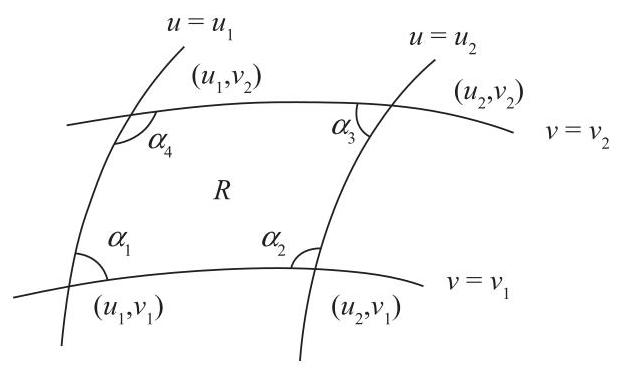
\includegraphics[max width=0.5\textwidth]{images/bo_d4b9jf3ef24c73e0334g_465_326_1025_619_372_0.jpg}
\end{center}
\hspace*{3em} 

图 5-54

到目前为止的考虑都是局部的.我们现在将定义一个映射 \(\mathbf{x} : {R}^{2} \rightarrow  {S}^{\prime }\) ，并证明 \(\mathbf{x}\) 是整个 \({S}^{\prime }\) 的一个参数化.

地图 \(\mathbf{x}\) 定义如下(图 5-55).固定一点 \(O \in  {S}^{\prime }\) ，并选择通过 \(O\) 的渐近曲线上的方向.明确选择其中一条渐近曲线，称之为 \({a}_{1}\) ，另一条记为 \({a}_{2}\) .对于每个 \(\left( {s,t}\right)  \in  {R}^{2}\) ，在 \({a}_{1}\) 上从 \(O\) 开始量取长度等于 \(s\) .设 \({p}^{\prime }\) 为由此得到的点.通过 \({p}^{\prime }\) 有两条渐近曲线，其中一条是 \({a}_{1}\) .选择另一条，并赋予它通过沿 \({a}_{1}\) 的连续延伸得到的方向，该方向是 \({a}_{2}\) 的方向.在这条有方向的渐近曲线上，从 \({p}^{\prime }\) 开始量取长度等于 \(t\) .由此得到的点是 \(\mathbf{x}\left( {s,t}\right)\) .

\(\mathbf{x}\left( {s,t}\right)\) 对于所有 \(\left( {s,t}\right)  \in  {R}^{2}\) 都是良定义的.事实上，如果 \(\mathbf{x}\left( {s,0}\right)\) 未定义，则存在 \({s}_{1}\) 使得对于所有 \(s < {s}_{1}\)  \({a}_{1}\left( s\right)\) 都定义，但对于 \(s = {s}_{1}\) 未定义.设 \(q = \mathop{\lim }\limits_{{s \rightarrow  {s}_{1}}}{a}_{1}\left( s\right)\) .根据完备性， \(q \in  {S}^{\prime }\) .通过使用引理 2，我们看到 \({a}_{1}\left( {s}_{1}\right)\) 是定义的，这是一个矛盾，表明对于所有 \(s \in  R\)  \(\mathbf{x}\left( {s,0}\right)\) 都是定义的.用同样的论证，我们证明了对于所有 \(t \in  R\)  \(\mathbf{x}\left( {s,t}\right)\) 都是定义的.

\begin{center}
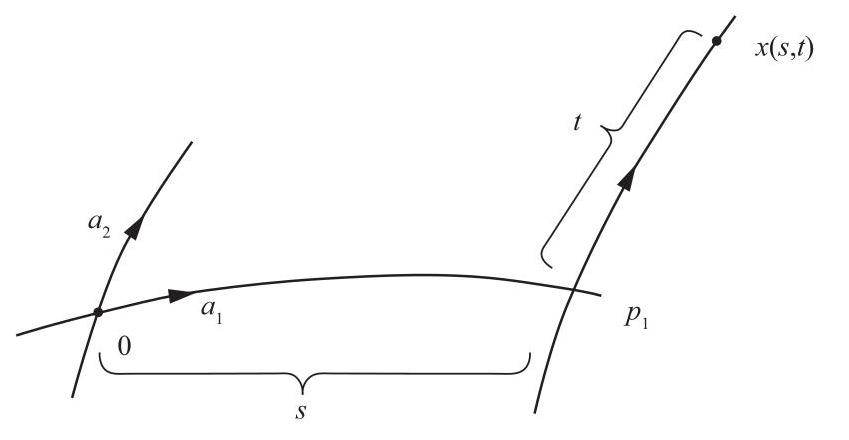
\includegraphics[max width=0.7\textwidth]{images/bo_d4b9jf3ef24c73e0334g_466_193_191_849_440_0.jpg}
\end{center}
\hspace*{3em} 

图 5-55

现在我们必须证明 \(\mathbf{x}\) 是 \({S}^{\prime }\) 的参数化.这将通过一系列引理来完成.

引理 4. 对于固定的 \(\mathrm{t}\) ，曲线 \(\mathbf{x}\left( {S,\mathrm{t}}\right) , - \infty  < s < \infty\) 是一条渐近曲线，其弧长为 \(S\) .

证明. 对于每一点 \(\mathbf{x}\left( {{s}^{\prime },{t}^{\prime }}\right)  \in  {S}^{\prime }\) ，根据引理 2，存在一个“矩形”邻域(即形式为 \({t}_{a} < t < {t}_{b},{s}_{a} < s < {s}_{b}\) 的邻域)，使得该邻域的渐近线构成切比雪夫网. 我们首先注意到，如果对于某个 \({t}_{0},{t}_{a} < {t}_{0} < {t}_{b}\) ，曲线 \(\mathbf{x}\left( {s,{t}_{0}}\right) ,{s}_{a} < s < {s}_{b}\) 是一条渐近线，那么我们知道对于每条曲线 \(\mathbf{x}\left( {s,\bar{t}}\right)\) ， \({t}_{a} < \bar{t} < {t}_{b}\) 也是如此. 事实上，点 \(\mathbf{x}\left( {s,\bar{t}}\right)\) 是通过从 \(\mathbf{x}\left( {s,0}\right)\) 处量出长度为 \(\bar{t}\) 的线段得到的，这等同于从 \(\mathbf{x}\left( {s,{t}_{0}}\right)\) 处量出长度为 \(\bar{t} - {t}_{0}\) 的线段. 由于渐近线在该邻域中构成切比雪夫网，因此该论断成立.

现在，设 \(\mathbf{x}\left( {{s}_{1},{t}_{1}}\right)  \in  {S}^{\prime }\) 为任意一点. 由于线段 \(\mathbf{x}\left( {{s}_{1},t}\right) ,0 \leq  t \leq  {t}_{1}\) 的紧致性，可以用有限个矩形邻域覆盖它，使得每个邻域的渐近线构成切比雪夫网(图 5-56). 由于 \(\mathbf{x}\left( {s,0}\right)\) 是一条渐近线，我们重复之前的论述，并证明 \(\mathbf{x}\left( {s,{t}_{1}}\right)\) 在 \({s}_{1}\) 的邻域中是一条渐近线. 由于 \(\left( {{s}_{1},{t}_{1}}\right)\) 是任意的，引理的论断成立. 证毕.

\section*{引理 5. \(\mathbf{x}\) 是一个局部微分同胚.}

证明. 这是因为一方面 \(\mathbf{x}\left( {{s}_{0},t}\right) ,\mathbf{x}\left( {s,{t}_{0}}\right)\) 是由弧长参数化的渐近线，另一方面 \({S}^{\prime }\) 可以局部参数化，使得坐标曲线是 \({S}^{\prime }\) 和 \(E = G = 1\) 的渐近线. 因此， \(\mathbf{x}\) 在局部上与这种参数化一致.

\begin{center}
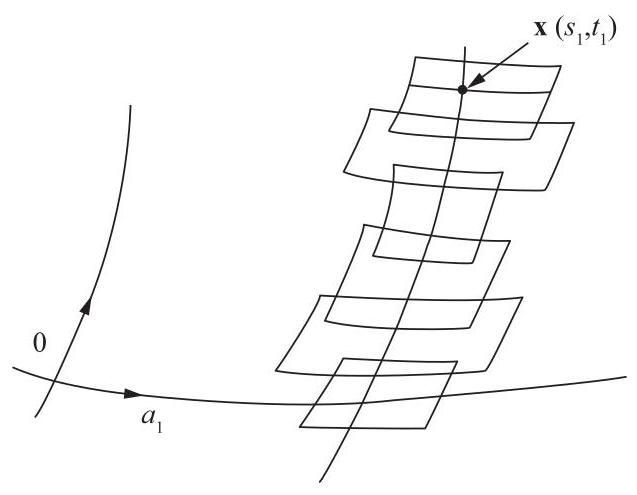
\includegraphics[max width=0.5\textwidth]{images/bo_d4b9jf3ef24c73e0334g_467_180_193_637_495_0.jpg}
\end{center}
\hspace*{3em} 

图 5-56

引理 6. \(\mathbf{x}\) 是满射.

证明. 设 \(Q = \mathbf{x}\left( {R}^{2}\right)\) . 由于 \(\mathbf{x}\) 是一个局部微分同胚， \(Q\) 在 \({S}^{\prime }\) 中是开集. 我们还注意到，如果 \({p}^{\prime } = \mathbf{x}\left( {{s}_{0},{t}_{0}}\right)\) ，那么通过 \({p}^{\prime }\) 的两条渐近线完全包含在 \(Q\) 中.

假设 \(Q \neq  {S}^{\prime }\) .由于 \({S}^{\prime }\) 是连通的，边界 Bd \(Q \neq  \phi\) .令 \(p \in  \mathrm{{Bd}}Q\) .由于 \(Q\) 在 \({S}^{\prime },p \notin  Q\) 中是开集.现在考虑 \(p\) 的一个矩形邻域 \(R\) ，其中渐近线构成一个切比雪夫网(图 5-57).令 \(q \in  Q \cap  R\) .那么通过 \(q\) 的一条渐近线与通过 \(p\) 的一条渐近线相交.根据上述评论，这是矛盾的.证毕.

\begin{center}
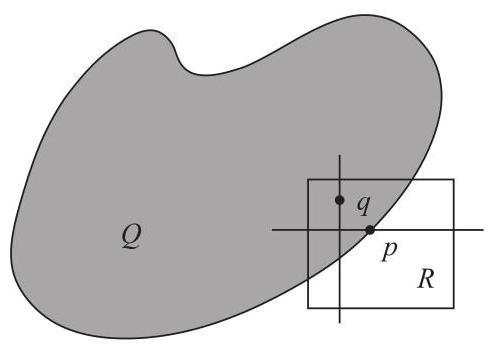
\includegraphics[max width=0.4\textwidth]{images/bo_d4b9jf3ef24c73e0334g_467_182_1247_495_350_0.jpg}
\end{center}
\hspace*{3em} 

图 5-57

我们现在声称 \(\mathbf{x}\) 是一个全局微分同胚.由于 \(\mathbf{x}\) 是一个满射局部微分同胚，因此只需证明 \(x\) 具有提升弧的性质，并应用第 5-6 节的命题 6(覆盖空间...)来得出 \(\mathbf{x}\) 是一个覆盖映射.由于 \({R}^{2}\) 是单连通的，这将证明我们的主张.

为了证明 \(\mathbf{x}\) 具有提升弧的性质，我们使用一个在此未加证明的命题(证明请参见 Elon Lima 的《基本群与覆盖空间》，A K Peters 出版社，马萨诸塞州纳蒂克，第 144 页):...令 \(\mathbf{x} : {\mathbb{R}}^{2} \rightarrow  {S}^{\prime }\) 为一个满射局部微分同胚.假设 \(\mathbf{x}\) 是一个闭映射(即闭集的像也是闭集).那么 \(\mathbf{x}\) 具有提升弧的性质. \(\mathbf{x}\) 是闭映射是根据其定义方式得出的.

这就完成了我们主张的证明.

希尔伯特定理的证明现在可以轻松得出.

定理证明.假设存在一个等距浸入 \(\psi  : S \rightarrow  {R}^{3}\) ，其中 \(S\) 是一个具有 \(K \equiv   - 1\) 的完备曲面.令 \(p \in  S\) 并将 \({S}^{\prime }\) 表示为切平面 \({T}_{p}\left( S\right)\) ，其上带有由 \({\exp }_{p} : {T}_{p}\left( S\right)  \rightarrow  S\) 诱导的度量.那么 \(\varphi  = \psi  \circ  {\exp }_{p} : {S}^{\prime } \rightarrow  {R}^{3}\) 是一个等距浸入，引理 5 和 6 以及它们之后的文本表明存在一个 \({S}^{\prime }\) 的参数化 \(\mathbf{x} : {R}^{2} \rightarrow  {S}^{\prime }\) ，使得 \(\mathbf{x}\) 的坐标曲线是 \({S}^{\prime }\) 的渐近曲线(引理 4).因此，我们可以用一组“坐标四边形” \({Q}_{n}\) 来覆盖 \({S}^{\prime }\) ，其中 \({Q}_{n} \subset  {Q}_{n + 1}\) .根据引理 3，每个 \({Q}_{n}\) 的面积小于 \({2\pi }\) .另一方面，根据引理 1， \({S}^{\prime }\) 的面积是无界的.这是矛盾的，证明结束.证毕.

注记 2.希尔伯特定理由 N. V. Efimov 在“负曲率曲面上的奇点出现”一文中推广，该文发表于 Math. Sb. 106 (1954).A.M.S. Translations. Series 2, Vol. 66, 1968, 154-190.他证明了 Cohn-Vossen 的以下猜想:设 S 是一个具有曲率 \(\mathrm{K}\) 且满足 \(\mathrm{K} \leq  \delta  < 0\) 的完备曲面.那么不存在 S 到 \({\mathbb{R}}^{3}\) 的等距浸入.Efimov 的证明非常冗长，因此需要一个更简短的证明.

Efimov 证明的一个精彩阐述可以在 T. Klotz Milnor 的论文 "Efimov's Theorem About Complete Immersed Surfaces of Negative Curvature," Advances in Mathematics 8 (1972), 474-543 中找到.该论文还包含 Hilbert 定理的另一个证明，该定理适用于 \({C}^{2}\) 类曲面.

关于双曲平面浸入的更多细节，请参阅 M. L. Cromov 和 V. A. Rokblin 的论文 "Embeddings and Immersions in Riemannian Geometry," Russian Math. Sureys (1970), 1-57，特别是第 15 页.

\exerciseline

1. (Stoke 的注记.) 令 \(S\) 为一个完备的几何曲面.假设高斯曲率 \(K\) 满足 \(K \leq  \delta  < 0\) .证明不存在一个平均曲率 \(H\) 的绝对值有界的等距浸入 \(\varphi  : S \rightarrow  {R}^{3}\) .这证明了注记 2 中引用的 Efimov 定理，并加上了平均曲率的附加条件.以下大纲可能有用:

a. 假设存在这样的 \(\varphi\) ，并考虑高斯映射 \(N : \varphi \left( S\right)  \subset  {R}^{3} \rightarrow \; {S}^{2}\) ，其中 \({S}^{2}\) 是单位球面.由于 \(K \neq  0\) 处处存在， \(N\) 通过要求 \(N \circ  \varphi  : S \rightarrow  {S}^{2}\) 是局部等距映射，在 \(S\) 上诱导出一个新的度量 (, ) .在 \(S\) 上选择坐标，使得 \(\varphi\) 的坐标曲线的像成为 \(\varphi \left( S\right)\) 的曲率线.证明在这个坐标系中，新度量的系数是

\[
{g}_{11} = {\left( {k}_{1}\right) }^{2}E,\;{g}_{12} = 0,\;{g}_{22} = {\left( {k}_{2}\right) }^{2}G,
\]

其中 \(E,F\left( { = 0}\right)\) 和 \(G\) 是同一坐标系中初始度量的系数.

b. 证明存在一个常数 \(M > 0\) ，使得 \({k}_{1}^{2} < M,{k}_{2}^{2} < M\) .利用初始度量是完备的事实，得出新度量也是完备的.

c. 利用 b 部分证明 \(S\) 是紧致的；因此，它存在曲率为正的点，这是一个矛盾.

2. 本练习的目的是证明在 \({R}^{3}\) 中不存在具有 \(K \leq  \delta  < 0\) 的正则完备旋转曲面 \(S\) (这证明了 Efimov 定理对旋转曲面成立).假设存在这样一个 \(S \subset  {R}^{3}\) .

a. 证明 \(S\) 的生成曲线的唯一可能形式是图 5-58(a) 和 (b) 中的形式，其中子午线向两个方向延伸至无穷.注意，在图 5-58(b) 中，子午线的下半部分渐近于 \(z\) 轴.

b. 用弧长 \(s \in  R\) 参数化生成曲线 \(\left( {\varphi \left( s\right) ,\psi \left( s\right) }\right)\) ，使得 \(\psi \left( 0\right)  = 0\) .利用关系式 \({\varphi }^{\prime \prime } + {K\varphi } = 0\) (参见例 4，第 3-3 节，方程 (9))和 \(K \leq  \delta  < 0\) 得出存在一点 \({s}_{0} \in  \lbrack 0, + \infty )\) ，使得 \({\left( {\varphi }^{\prime }\left( {s}_{0}\right) \right) }^{2} = 1\) .

c. 证明继续子午线 \(\left( {\varphi \left( s\right) ,\psi \left( s\right) }\right)\) 越过 \(S\) 点 \({p}_{0} = \left( {\varphi \left( {s}_{0}\right) ,\psi \left( {s}_{0}\right) }\right)\) 的三种可能(如图 5-58(c) 所示的 I、II 和 III)都导致矛盾.因此， \(S\) 不是完备的.

3. (T. K. Milnor 的希尔伯特定理证明.) 令 \(S\) 为一个具有完备度量 \({g}_{1}\) 的平面，其曲率 \(K \equiv   - 1\) .假设存在一个等距浸入 \(\varphi  : S \rightarrow  {R}^{3}\) .为得到矛盾，按以下步骤进行:

\begin{center}
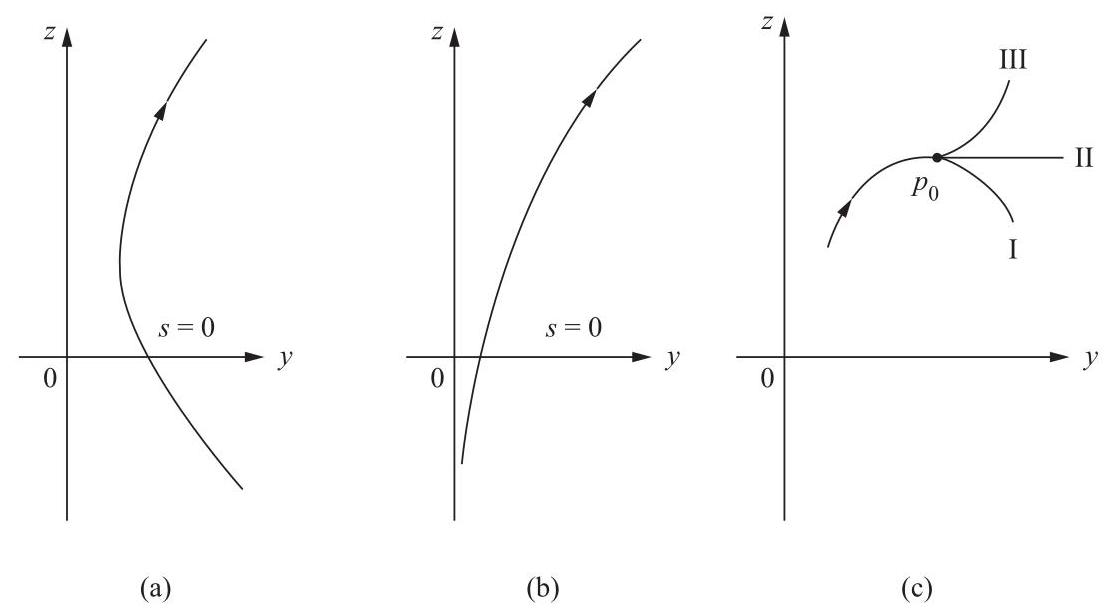
\includegraphics[max width=1.0\textwidth]{images/bo_d4b9jf3ef24c73e0334g_469_209_1428_1115_616_0.jpg}
\end{center}
\hspace*{3em} 

图 5-58

a. 考虑高斯映射 \(N : \varphi \left( S\right)  \subset  {R}^{3} \rightarrow  {S}^{2}\) ，令 \({g}_{2}\) 为 \(S\) 上的度量，通过要求 \(N \circ  \varphi  : S \rightarrow  {S}^{2}\) 为局部等距来实现.在 \(S\) 上选择局部坐标，使得坐标曲线经 \(\varphi\) 映射到 \(\varphi \left( S\right)\) 的渐近曲线.证明在此坐标系下， \({g}_{1}\) 可写为

\[
d{u}^{2} + 2\cos {\theta dudv} + d{v}^{2}
\]

并且 \({g}_{2}\) 可写为

\[
d{u}^{2} - 2\cos {\theta dudv} + d{v}^{2}.
\]

b. 证明 \({g}_{3} = \frac{1}{2}\left( {{g}_{1} + {g}_{2}}\right)\) 是 \(S\) 上一个曲率为零的度量.利用 \({g}_{1}\) 是完备度量且 \(3{g}_{3} \geq  {g}_{1}\) 的事实，得出度量 \({g}_{3}\) 是完备的.

c. 证明具有度量 \({g}_{3}\) 的平面与标准(欧几里得)平面 \({R}^{2}\) 全局等距.因此，存在一个等距映射 \(\varphi  : S \rightarrow  {R}^{2}\) .进一步证明 \(\varphi\) 将由弧长参数化的 \(S\) 的渐近曲线映射到 \({R}^{2}\) 中一个由弧长参数化的直线的矩形系统.

d. 利用 c 部分给出的 \(S\) 上的全局坐标系，并如文本中希尔伯特定理的证明那样得到一个矛盾.

附录 欧几里得空间的点集拓扑

在第 5 章中，我们更自由地使用了一些 \({R}^{n}\) 的基本拓扑性质.通常在高等微积分课程中出现的紧致和连通子集的性质，基本上就是所需要的全部.为完整起见，我们将在此简要介绍这些材料，并附带证明.我们将假定第 2 章附录 A 的材料以及实数的基本性质.

\section*{A. 预备知识}

在此，我们将补充第 2 章附录 A 的部分内容.

在下文中， \(U \subset  {R}^{n}\) 将表示 \({R}^{n}\) 中的一个开集.下标 \(i\) 在范围 \(1,2,\ldots ,m,\ldots\) 内变化，如果 \(p = \left( {{x}_{1},\ldots ,{x}_{n}}\right) ,q = \left( {{y}_{1},\ldots ,{y}_{n}}\right) ,\left| {p - q}\right|\) 将表示从 \(p\) 到 \(q\) 的距离；即，

\[
{\left| p - q\right| }^{2} = \mathop{\sum }\limits_{j}{\left( {x}_{j} - {y}_{j}\right) }^{2},\;j = 1,\ldots ,n.
\]

定义 1. 如果给定 \(\epsilon  > 0\) ，存在一个序列的索引 \({\mathrm{i}}_{0}\) 使得对于所有 \(\mathrm{i} > {\mathrm{i}}_{0}\) 都有 \({\mathrm{p}}_{1} \in  {\mathrm{B}}_{\epsilon }\left( {\mathrm{p}}_{0}\right)\) ，则称序列 \({\mathrm{p}}_{1},\ldots ,{\mathrm{p}}_{\mathrm{i}},\ldots  \in  {\mathbb{R}}^{N}\) 收敛于 \({\mathrm{p}}_{0} \in  {\mathbb{R}}^{N}\) .在这种情况下， \({\mathrm{p}}_{0}\) 是序列 \(\left\{  {\mathrm{p}}_{1}\right\}\) 的极限，记作 \(\left\{  {\mathrm{p}}_{\mathrm{i}}\right\}   \rightarrow  {\mathrm{p}}_{0}\) .

收敛性与连续性通过以下命题相关联.

命题 1. 如果且仅当对于 \(\mathrm{U}\) 中的每个收敛序列 \(\left\{  {\mathrm{p}}_{\mathrm{i}}\right\}   \rightarrow  {\mathrm{p}}_{0}\) ，序列 \(\left\{  {\mathrm{F}\left( {\mathrm{p}}_{\mathrm{i}}\right) }\right\}\) 收敛于 \(\mathrm{F}\left( {\mathrm{p}}_{0}\right)\) ，则映射 F: \(\mathrm{U} \subset  {\mathbb{R}}^{N} \rightarrow  {\mathrm{F}}^{\mathrm{m}}\) 在 \({\mathrm{p}}_{0} \in  \mathrm{U}\) 处是连续的.

证明.假设 \(F\) 在 \({p}_{0}\) 处连续，并给定 \(\epsilon  > 0\) .根据连续性，存在 \(\delta  > 0\) 使得 \(F\left( {{B}_{\delta }\left( {p}_{0}\right) }\right)  \subset  {B}_{\epsilon }\left( {F\left( {p}_{0}\right) }\right)\) .设 \(\left\{  {p}_{1}\right\}\) 是 \(U\) 中的一个序列，且 \(\left\{  {p}_{i}\right\}   \rightarrow  {p}_{0} \in  U\) .那么，与 \(\delta\) 对应存在一个索引 \({i}_{0}\) 使得对于 \(i > {i}_{0}\) 有 \({p}_{i} \in  {B}_{\delta }\left( {p}_{0}\right)\) .因此，对于 \(i > {i}_{0}\) ，

\[
F\left( {p}_{i}\right)  \in  F\left( {{B}_{\delta }\left( {p}_{0}\right) }\right)  \subset  {B}_{\epsilon }\left( {F\left( {p}_{0}\right) }\right) ,
\]

这蕴含着 \(\left\{  {F\left( {p}_{1}\right) }\right\}   \rightarrow  F\left( {p}_{0}\right)\) .

假设现在 \(F\) 在 \({p}_{0}\) 处不连续.那么存在一个数 \(\epsilon  > 0\) ，使得对于每一个 \(\delta  > 0\) 都可以找到一个点 \(p \in  {B}_{\delta }\left( {p}_{0}\right)\) ，满足 \(F\left( p\right)  \notin  {B}_{\epsilon }\left( {F\left( {p}_{0}\right) }\right)\) .固定这个 \(\epsilon\) ，并令 \(\delta  = 1,1/2,\ldots ,1/i,\ldots\) ，从而得到一个收敛于 \({p}_{0}\) 的序列 \(\left\{  {p}_{i}\right\}\) .然而，由于 \(F\left( {p}_{i}\right)  \notin  {B}_{\epsilon }\left( {F\left( {p}_{0}\right) }\right)\) ，序列 \(\left\{  {F\left( {p}_{i}\right) }\right\}\) 不收敛于 \(F\left( {p}_{0}\right)\) .Q.E.D.

定义 2. 如果 \({\mathbb{R}}^{N}\) 中的 \({\mathbb{R}}^{N}\) 的每个邻域都包含 \(\mathrm{A}\) 中不同于 \(\mathrm{p}\) 的一个点，则称点 \(\mathrm{p} \in  {\mathbb{R}}^{N}\) 是集合 \(\mathrm{A} \subset  {\mathbb{R}}^{N}\) 的极限点.

为了避免与序列极限的概念混淆，极限点有时被称为聚点或累积点.

定义 2 等价于说 \(p\) 的每个邻域 \(V\) 都包含 \(A\) 的无穷多个点.事实上，设 \({q}_{1} \neq  p\) 是定义给出的 \(A\) 中的点，并考虑一个球 \({B}_{\epsilon }\left( p\right)  \subset  V\) 使得 \({q}_{1} \notin  {B}_{\epsilon }\left( p\right)\) .那么存在一个点 \({q}_{2} \neq  p,{q}_{2} \in  A \cap  {B}_{\epsilon }\left( p\right)\) .通过重复这个过程，我们在 \(V\) 中得到一个序列 \(\left\{  {q}_{i}\right\}\) ，其中 \({q}_{1} \in  A\) 都不同.由于 \(\left\{  {q}_{t}\right\}   \rightarrow  p\) ，该论证也表明 \(p\) 是 \(A\) 的极限点当且仅当 \(p\) 是 \(A\) 中某个不同点序列的极限.

例 1. 序列 \(1,1/2,1/3,\ldots ,1/i,\ldots\) 收敛于 0.序列 \(3/2,4/3,\ldots ,i + 1/i,\ldots\) 收敛于 1.“交织”序列 \(1,3/2,1/2,4/3,1/3,\ldots ,1 + \left( {1/i}\right) ,1/i,\ldots\) 不收敛，有两个极限点，即 0 和 1(图 A5-1).

\begin{center}
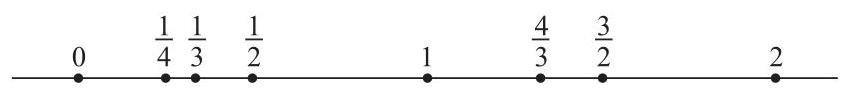
\includegraphics[max width=0.7\textwidth]{images/bo_d4b9jf3ef24c73e0334g_472_361_1541_852_95_0.jpg}
\end{center}
\hspace*{3em} 

图 A5-1

应该注意到，收敛序列的极限 \({p}_{0}\) 具有这样的性质: \({p}_{0}\) 的任何邻域都包含该序列除有限个点之外的所有点，而集合的极限点 \(p\) 具有一个较弱的性质: \(p\) 的任何邻域都包含该集合的无穷多个点.因此，一个不包含常数子序列的序列是收敛的当且仅当它作为一个集合只包含一个极限点.

一个有趣的例子是给出有理数 \(Q\) .可以证明 \(Q\) 是可数的；也就是说，它可以构成一个序列.由于在任何实数附近都有有理数，序列 \(Q\) 的极限点集是实轴 \(R\) .

定义 3. 如果 \(\mathrm{F}\) 的每个极限点都属于 \(\mathrm{F}\) ，则称集合 \(\mathrm{F} \subset  {\mathbb{R}}^{N}\) 是闭集. \(\mathrm{A} \subset  {\mathbb{R}}^{N}\) 的闭包，记作 \(\bar{\mathrm{A}}\) ，是 \(\mathrm{A}\) 与其极限点的并集.

直观地说，如果一个集合 \(F\) 包含其所有收敛序列的极限，或者换句话说，它在取极限的过程中是不变的，那么它就是闭集.

显然，一个集合的闭包是一个闭集.为了方便起见，我们约定空集 \(\phi\) 既是开集也是闭集.

开集和闭集之间存在一个非常简单的关系.

命题 2. 如果 \(\mathrm{F}\) 的补集 \({\mathbb{R}}^{N} - \mathrm{F}\) 是开集，则 \(\mathrm{F} \subset  {\mathbb{R}}^{N}\) 是闭集，反之亦然.

证明. 假设 \(F\) 是闭集且 \(p \in  {R}^{n} - F\) . 由于 \(p\) 不是 \(F\) 的极限点，存在一个球 \({B}_{\epsilon }\left( p\right)\) 不包含 \(F\) 的任何点. 因此， \({B}_{\epsilon } \subset  {R}^{n} - F\) ；所以 \({R}^{n} - F\) 是开集.

反之，假设 \({R}^{n} - F\) 是开集且 \(p\) 是 \(F\) 的极限点. 我们要证明 \(p \in  F\) . 假设相反. 那么存在一个球 \({B}_{\epsilon }\left( p\right)  \subset \; {R}^{n} - F\) . 这意味着 \({B}_{\epsilon }\left( p\right)\) 不包含 \(F\) 的任何点，这与 \(p\) 是 \(F\) 的极限点的这个事实相矛盾.Q.E.D.

连续性也可以用闭集来表示，这是以下事实的推论.

命题 3. 映射 F: \(\mathrm{U} \subset  {\mathbb{R}}^{N} \rightarrow  {\mathbb{R}}^{\mathrm{m}}\) 是连续的，当且仅当对于每个开集 \(\mathrm{V} \subset  {\mathbb{R}}^{\mathrm{m}},{\mathrm{F}}^{-1}\left( \mathrm{\;V}\right)\) 都是开集.

证明. 假设 \(F\) 是连续的，令 \(V \subset  {R}^{m}\) 为 \({R}^{m}\) 中的一个开集. 如果 \({F}^{-1}\left( V\right)  = \phi\) ，则无需证明，因为我们约定空集是开集. 如果 \({F}^{-1}\left( V\right)  \neq  \phi\) ，令 \(p \in  {F}^{-1}\left( V\right)\) . 那么 \(F\left( p\right)  \in  V\) ，并且由于 \(V\) 是开集，存在一个球 \({B}_{\epsilon }\left( {F\left( p\right) }\right)  \subset  V\) . 由于 \(F\) 的连续性，存在一个球 \({B}_{\delta }\left( p\right)\) 使得

\[
F\left( {{B}_{\delta }\left( p\right) }\right)  \subset  {B}_{\epsilon }\left( {F\left( p\right) }\right)  \subset  V.
\]

因此， \({B}_{\delta }\left( p\right)  \subset  {F}^{-1}\left( V\right)\) ；所以， \({F}^{-1}\left( V\right)\) 是开集.

现在假设对于每个开集 \(V \subset  {R}^{m}\) ， \({F}^{-1}\left( V\right)\) 都是开集. 令 \(p \in  U\) 和 \(\epsilon  > 0\) 给定. 那么 \(A = {F}^{-1}\left( {{B}_{\epsilon }\left( {F\left( p\right) }\right) }\right)\) 是开集. 因此，存在 \(\delta  > 0\) 使得 \({B}_{\delta }\left( p\right)  \subset  A\) . 所以，

\[
F\left( {{B}_{\delta }\left( p\right) }\right)  \subset  F\left( A\right)  \subset  {B}_{\epsilon }\left( {F\left( p\right) }\right) ;
\]

因此， \(F\) 在 \(p\) 中是连续的.Q.E.D.

推论. F: \(\mathrm{U} \subset  {\mathbb{R}}^{N} \rightarrow  {\mathbb{R}}^{\mathrm{m}}\) 是连续的，当且仅当对于每个闭集 \(\mathrm{A} \subset  {\mathbb{R}}^{\mathrm{m}},{\mathrm{F}}^{-1}\left( \mathrm{\;A}\right)\) 是闭集.

命题 3 及其推论给出了描述 \({R}^{n}\) 的开集和闭集的最佳方法.例如，设 \(f : {R}^{2} \rightarrow  R\) 由 \(f\left( {x,y}\right)  = \left( {{x}^{2}/{a}^{2}}\right)  - \left( {{y}^{2}/{b}^{2}}\right)  - 1\) 给出.观察到 \(f\) 是连续的， \(0 \in  R\) 是 \(R\) 中的一个闭集，而 \(\left( {0, + \infty }\right)\) 是 \(R\) 中的一个开集.因此，集合

\[
{F}_{1} = \{ \left( {x,y}\right) ;f\left( {x,y}\right)  = 0\}  = {f}^{-1}\left( 0\right)
\]

在 \({R}^{2}\) 中是闭集，而集合

\[
{U}_{1} = \{ \left( {x,y}\right) ;f\left( {x,y}\right)  > 0\}
\]

\[
{U}_{2} = \{ \left( {x,y}\right) ;f\left( {x,y}\right)  < 0\}
\]

在 \({R}^{2}\) 中是开集.另一方面，集合

\[
A = \left\{  {\left( {x,y}\right)  \in  {R}^{2},{x}^{2} + {y}^{2} < 1}\right\}
\]

\[
\cup  \left\{  {\left( {x,y}\right)  \in  {R}^{2};{x}^{2} + {y}^{2} = 1,x > 0,y > 0}\right\}
\]

既不是开集也不是闭集(图 A5-2).

\begin{center}
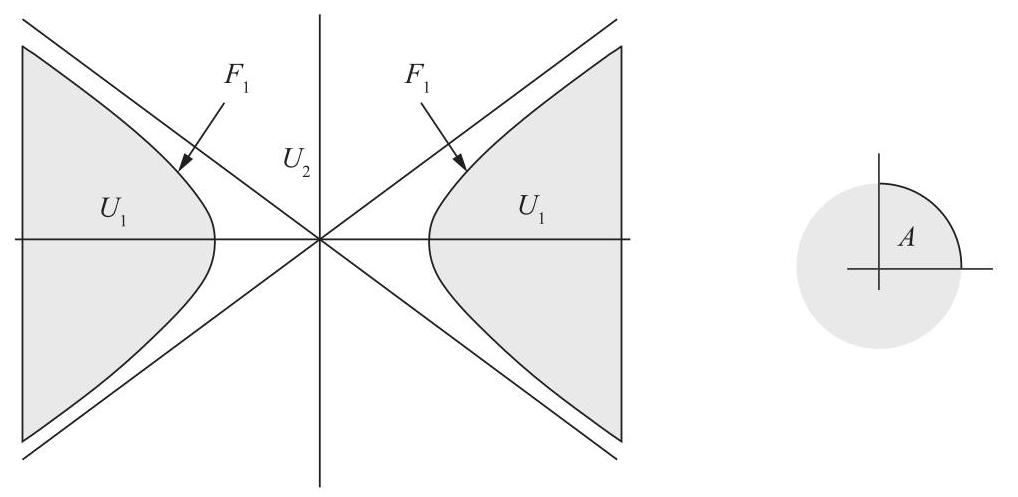
\includegraphics[max width=0.9\textwidth]{images/bo_d4b9jf3ef24c73e0334g_474_282_1123_1018_497_0.jpg}
\end{center}
\hspace*{3em} 

图 A5-2

最后一个例子提出了以下定义.

定义 4. 设 \(\mathrm{A} \subset  {\mathbb{R}}^{N}\) .集合 \(\mathrm{A}\) 在 \({\mathbb{R}}^{N}\) 中的边界 \(\mathrm{{Bd}}\) A 是指 \({\mathbb{R}}^{N}\) 中所有满足其任意邻域包含 \(\mathrm{A}\) 中的点和 \({\mathbb{R}}^{N} - \mathrm{A}\) 中的点的点 \(\mathrm{p}\) 的集合.

因此，如果 \(A\) 是例 2 的集合，则 Bd \(A\) 是圆 \({x}^{2} + {y}^{2} = 1\) .显然，当且仅当 Bd \(A\) 的点不属于 \(A\) 时， \(A \subset  {R}^{n}\) 是开集；当且仅当 Bd \(B\) 的所有点都属于 \(B\) 时， \(B \subset  {R}^{n}\) 是闭集.

现在我们回顾实数的某个基本性质.我们需要一些定义.

定义 5. 实轴 \(\mathbb{R}\) 的子集 \(\mathrm{A} \subset  \mathbb{R}\) 被称为有上界，如果存在 \(\mathrm{M} \in  \mathbb{R}\) 使得对于所有 \(\mathrm{a} \in  \mathrm{A}\) ，都有 \(\mathrm{M} \geq  \mathrm{a}\) .数 \(\mathrm{M}\) 被称为 A 的一个上界.当 A 有上界时，A 的上确界或最小上界，sup A(或 l.u.b. A)是满足以下条件的上界 M:给定 \(\epsilon  > 0\) ，存在一个 \(\in  \mathrm{A}\) 使得 \(\mathrm{M} - \epsilon  <\) a.通过改变上述不等式的符号，我们类似地定义了 A 的下界和下确界(或最大下界)，inf A(或 g.l.b. A).

实数完备性公理.设 \(\mathrm{A} \subset  \mathbb{R}\) 非空且有上界(下界).则存在 sup \(\mathrm{A}\) (inf \(\mathrm{A}\) ).

有几种等价的方式来表达实数系统的完备性的基本性质.我们选择了上述方式，虽然它不是最直观的，但可能是最有效的.

为了方便起见，我们设定以下约定.如果 \(A \subset  R\) 没有上界(下界)，我们说 sup \(A =  + \infty\) (inf \(A =  - \infty\) ).有了这个约定，上述公理可以表述为:每个非空实数集都有一个上确界和一个下确界.

例 3. 集合 \(\left( {0,1}\right)\) 的上确界是 1，它不属于该集合.集合

\[
B = \{ x \in  R;0 < x < 1\}  \cup  \{ 2\}
\]

2. 点 2 是 \(B\) 的孤立点；也就是说，它属于 \(B\) 但不是 \(B\) 的极限点.注意 \(B\) 的最大极限点是 1，它不是 \(B\) 的上确界.然而，如果一个有界集没有孤立点，它的上确界一定是该集的极限点.

实数完备性一个重要的推论是以下关于收敛的“内在”刻画，它实际上等价于完备性(然而，我们不证明这一点).

引理 1. 如果对于任意给定的 \(\epsilon  > 0\) ，都存在 \({\mathrm{i}}_{0}\) 使得对于所有 \(\mathrm{i},\mathrm{j} > {\mathrm{i}}_{0}\) 都有 \(\left| {{x}_{\mathrm{i}},{x}_{\mathrm{j}}}\right|  < \epsilon\) ，则称实数序列 \(\left\{  {x}_{i}\right\}\) 为柯西序列.一个序列收敛当且仅当它是一个柯西序列.

证明.设 \(\left\{  {x}_{i}\right\}   \rightarrow  {x}_{0}\) .那么，如果给定 \(\epsilon  > 0\) ，则存在 \({i}_{0}\) 使得对于 \(i > {i}_{0}\) 有 \(\left| {{x}_{i} - {x}_{0}}\right|  < \epsilon /2\) .因此，对于 \(i,j > {i}_{0}\) ，我们有

\[
\left| {{x}_{i} - {x}_{j}}\right|  \leq  \left| {{x}_{i} - {x}_{0}}\right|  + \left| {{x}_{j} - {x}_{0}}\right|  < \epsilon
\]

因此， \(\left\{  {x}_{i}\right\}\) 是一个柯西序列.

反之，设 \(\left\{  {x}_{i}\right\}\) 是一个柯西序列.集合 \(\left\{  {x}_{i}\right\}\) 显然是一个有界集.设 \({a}_{1} = \inf \{ x\} ,{b}_{1} = \sup \left\{  {x}_{i}\right\}\) .要么，其中一个点是 \(\left\{  {x}_{i}\right\}\) 的极限点，那么 \(\left\{  {x}_{i}\right\}\) 收敛于该点，要么这两个点都是集合 \(\left\{  {x}_{i}\right\}\) 的孤立点.在后一种情况下，考虑开区间 \(\left( {{a}_{1},{b}_{1}}\right)\) 中的点集，并设 \({a}_{2}\) 和 \({b}_{2}\) 分别是它的下确界和上确界.按此方式进行，我们得到 \(\left\{  {x}_{i}\right\}\) 收敛，或者存在两个有界序列 \({a}_{1} < {a}_{2} < \cdots\) 和 \({b}_{1} > {b}_{2} > \cdots\) .设 \(a = \sup \left\{  {a}_{i}\right\}\) 和 \(b = \inf \left\{  {b}_{i}\right\}\) .由于 \(\left\{  {x}_{i}\right\}\) 是一个柯西序列， \(a = b\) ，并且这个公共值 \({x}_{0}\) 是 \(\left\{  {x}_{i}\right\}\) 的唯一极限点.因此， \(\left\{  {x}_{i}\right\}   \rightarrow  {x}_{0}\) .Q.E.D.

这种形式的完备性自然地推广到欧几里得空间.

定义 6. 如果对于任意给定的 \(\epsilon  > 0\) ，都存在一个指标 \({\mathrm{i}}_{0}\) 使得对于所有 \(\mathrm{i},\mathrm{j} > {\mathrm{i}}_{0}\) 都有距离 \(\left| {{\mathrm{p}}_{\mathrm{i}} - {\mathrm{p}}_{\mathrm{j}}}\right|  < \epsilon\) ，则称序列 \(\left\{  {\mathrm{p}}_{\mathrm{i}}\right\}  ,{\mathrm{p}}_{\mathrm{i}} \in  {\mathbb{R}}^{N}\) 是一个柯西序列.

命题 4. 一个序列 \(\left\{  {\mathrm{p}}_{\mathrm{i}}\right\}  ,{\mathrm{p}}_{\mathrm{i}} \in  {\mathbb{R}}^{N}\) 收敛当且仅当它是一个柯西序列.

证明. 一个收敛序列显然是一个柯西序列(参见引理 1 中的论证).反之，设 \(\left\{  {p}_{i}\right\}\) 是一个柯西序列，并考虑它在 \({R}^{n},j = 1,\ldots ,n\) 的 \(j\) 轴上的投影.这得到一个实数序列 \(\left\{  {x}_{ji}\right\}\) ，由于投影减小了距离，它仍然是一个柯西序列.根据引理 \(1,\left\{  {x}_{ji}\right\}   \rightarrow  {x}_{j0}\) . 可知 \(\left\{  {p}_{i}\right\}   \rightarrow  {p}_{0} = \left\{  {{x}_{10},{x}_{20},\ldots ,{x}_{n0}}\right\}  .\)Q.E.D.

\section*{B. 连通集}

定义 7. 一个连续曲线 \(\alpha  : \left\lbrack  {\mathrm{a},\mathrm{b}}\right\rbrack   \rightarrow  \mathrm{A} \subset  {\mathbb{R}}^{N}\) 在 A 中连接 \(\alpha \left( \mathrm{a}\right)\) 和 \(\alpha \left( \mathrm{b}\right)\) 被称为弧.

定义 8. 如果给定 A 中的任意两点 \(\mathrm{p},\mathrm{q} \in\) ，存在一条连接 \(\mathrm{p}\) 和 q 的弧，则称 \(\mathrm{A} \subset  {\mathbb{R}}^{N}\) 是弧连通的.

本书前面我们用“连通”来表示“弧连通”(第 2-2 节).由于我们只考虑正则曲面，这可以被证明是合理的，稍后会进行说明.然而，对于 \({R}^{n}\) 的一般子集来说，弧连通的概念过于严格，使用以下定义更为方便.

定义 9. 当无法将 \(\mathrm{A} \subset  {\mathbb{R}}^{N}\) 写成 \(\mathrm{A} = {\mathrm{U}}_{1} \cup  {\mathrm{U}}_{2}\) 的形式时，称 \(\mathrm{A} \subset  {\mathbb{R}}^{N}\) 是连通的，其中 \({\mathrm{U}}_{1}\) 和 \({\mathrm{U}}_{2}\) 是 \(\mathrm{A}\) 中的非空开集，并且 \({\mathrm{U}}_{1} \cap  {\mathrm{U}}_{2} = \phi\) .

直观地说，这意味着无法将 \(A\) 分解成不相交的部分.例如，示例 2 中的集合 \({U}_{1}\) 和 \({F}_{1}\) 不是连通的.通过取 \({U}_{1}\) 和 \({U}_{2}\) 的补集，我们发现可以将定义 10 中的“开”替换为“闭”.

命题 5. 设 \(\mathrm{A} \subset  {\mathbb{R}}^{N}\) 是连通的，并且设 \(\mathrm{B} \subset  \mathrm{A}\) 在 \(\mathrm{A}\) 中既是开集又是闭集.则 \(\mathrm{B} = \phi\) 或 \(\mathrm{B} = \mathrm{A}\) .

证明. 假设 \(B \neq  \phi\) 和 \(B \neq  A\) 并且写成 \(A = B \cup  \left( {A - B}\right)\) .由于 \(B\) 在 \(A,A - B\) 中是闭集，则 \(A,A - B\) 在 \(A\) 中是开集.因此， \(A\) 是不相交的、非空的、开集的并集，即 \(B\) 和 \(A - B\) .这与 \(A\) 的连通性矛盾.

Q.E.D.

下一个命题表明连通集的连续像也是连通的.

命题 6. 设 \(\mathrm{F} : \mathrm{A} \subset  {\mathbb{R}}^{N} \rightarrow  {\mathbb{R}}^{\mathrm{m}}\) 是连续的，并且 \(\mathrm{A}\) 是连通的.则 \(\mathrm{F}\left( \mathrm{A}\right)\) 是连通的.

证明. 假设 \(F\left( A\right)\) 不是连通的.则 \(F\left( A\right)  = {U}_{1} \cup  {U}_{2}\) ，其中 \({U}_{1}\) 和 \({U}_{2}\) 是 \(F\left( A\right)\) 中不相交的、非空的、开集.由于 \(F\) 是连续的， \({F}^{-1}\left( {U}_{1}\right) ,{F}^{-1}\left( {U}_{2}\right)\) 也是 \(A\) 中不相交的、非空的、开集.由于 \(A = \; {F}^{-1}\left( {U}_{1}\right)  \cup  {F}^{-1}\left( {U}_{2}\right)\) ，这与 \(A\) 的连通性矛盾.

为了本节的方便，我们将区间定义扩展如下:

定义 10. 实轴上的区间 \(\mathbb{R}\) 是指集合 \(\mathrm{a} < \; x < b,a \leq  x \leq  b,a < x \leq  b,a \leq  x < b,x \in  R\) 中的任意一个.区间可以是点、半直线或 R 本身，因此 \(a = b,a =  - \infty\) 、 \(\mathrm{b} =  + \infty\) 的情况并不排除.

命题 7. \(\subset  \mathbb{R}\) 是连通的，当且仅当 \(\mathrm{A}\) 是一个区间.

证明. 设 \(A \subset  R\) 是一个区间，并假设 \(A\) 不是连通的.我们将得出矛盾.

由于 \(A\) 不是连通的，则存在 \(A = {U}_{1} \cup  {U}_{2}\) ，其中 \({U}_{1}\) 和 \({U}_{2}\) 是非空、不相交且在 \(A\) 中是开集.设 \({a}_{1} \in  {U}_{1},{b}_{1} \in  {U}_{2}\) ，并假设 \({a}_{1} < {b}_{1}\) .通过将闭区间 \(\left\lbrack  {{a}_{1},{b}_{1}}\right\rbrack   = {I}_{1}\) 除以中点 \(\left( {{a}_{1} + {b}_{1}}\right) /2\) ，我们得到两个区间，其中一个区间(记为 \({I}_{2}\) )的一个端点在 \({U}_{1}\) 中，另一个端点在 \({U}_{2}\) 中.考虑 \({I}_{2}\) 的中点并重复上述过程，我们得到一个区间 \({I}_{3} \subset  {I}_{2} \subset  {I}_{1}\) .因此，我们得到一个闭区间族 \({I}_{1} \supset  {I}_{2} \supset  \cdots  \supset  {I}_{n} \supset  \cdots\) ，其长度趋近于零.重写 \({I}_{i} = \left\lbrack  {{c}_{i},{d}_{i}}\right\rbrack\) .则 \({c}_{1} \leq  {c}_{2} \leq  \cdots  \leq  {c}_{n} \leq  \cdots\) ，并且 \({d}_{1} \geq  {d}_{2} \geq  \cdots  \geq  {d}_{n} \geq  \cdots\) .设 \(c = \sup \left\{  {c}_{1}\right\}\) 和 \(d = \inf \left\{  {d}_{i}\right\}\) .由于 \({d}_{1} - {c}_{i}\) 任意小，则 \(c = d\) .此外， \(c\) 的任何邻域都包含某个 \({I}_{i}\) ，当 \(i\) 足够大时.因此， \(c\) 是 \({U}_{1}\) 和 \({U}_{2}\) 的极限点.由于 \({U}_{1}\) 和 \({U}_{2}\) 是闭集，则 \(c \in  {U}_{1} \cap  {U}_{2}\) ，这与 \({U}_{1}\) 和 \({U}_{2}\) 的不相交性矛盾.

反之，假设 \(A\) 是连通的.如果 \(A\) 只包含一个元素，那么 \(A\) 是一个平凡的区间.假设 \(A\) 至少包含两个元素，令 \(a = \inf A\) , \(b = \sup A,a \neq  b\) .显然， \(A \subset  \left\lbrack  {a,b}\right\rbrack\) .我们将证明 \(\left( {a,b}\right)  \subset  A\) ，这就意味着 \(A\) 是一个区间.假设相反的情况；也就是说，存在 \(t\) , \(a < t < b\) ，使得 \(t \notin  A\) .集合 \(A \cap  \left( {-\infty ,t}\right)  = {V}_{1},A \cap  \left( {t, + \infty }\right)  = {V}_{2}\) 在 \(A = {V}_{1} \cup  {V}_{2}\) 中是开集.由于 \(A\) 是连通的，这些集合中的一个，例如 \({V}_{2}\) ，是空的.由于 \(b \in  \left( {t, + \infty }\right)\) ，这同时意味着 \(b \notin  A\) 并且 \(b\) 不是 \(A\) 的极限点.这与 \(b = \sup A\) 的事实相矛盾.同理，如果 \({V}_{1} = \phi\) ，我们将得到一个与 \(a = \inf A\) 的事实相矛盾的结论.Q.E.D.

命题 8.设 \(\mathrm{f} : \mathrm{A} \subset  {\mathbb{R}}^{N} \rightarrow  \mathbb{R}\) 是连续的， \(\mathrm{A}\) 是连通的.假设对于所有 \(\mathrm{q} \in  \mathrm{A}\) 都有 \(\mathrm{f}\left( \mathrm{q}\right)  \neq  0\) .那么 \(\mathrm{f}\) 在 A 中不改变符号.

证明.根据命题 6， \(f\left( A\right)  \subset  R\) 是连通的.根据命题 7， \(f\left( A\right)\) 是一个区间.根据假设， \(f\left( A\right)\) 不包含零.因此， \(f\left( A\right)\) 中的点都具有相同的符号.证毕.

命题 9.设 \(\mathrm{A} \subset  {\mathbb{R}}^{N}\) 是弧状连通的.那么 \(\mathrm{A}\) 是连通的.

证明.假设 \(A\) 是不连通的.那么 \(A = {U}_{1} \cup  {U}_{2}\) ，其中 \({U}_{1}\) , \({U}_{2}\) 是非空、不相交的开集，在 \(A\) 中.令 \(p \in  {U}_{1},q \in  {U}_{2}\) .由于 \(A\) 是弧状连通的，存在一条弧 \(\alpha  : \left\lbrack  {a,b}\right\rbrack   \rightarrow  A\) 连接 \(p\) 和 \(q\) .由于 \(\alpha\) 是连续的， \(B = \alpha \left( \left\lbrack  {a,b}\right\rbrack  \right)  \subset  A\) 是连通的.令 \({V}_{1} = B \cap  {U}_{1},{V}_{2} = B \cap  {U}_{2}\) .那么 \(B = {V}_{1} \cup  {V}_{2}\) ，其中 \({V}_{1}\) 和 \({V}_{2}\) 是非空、不相交的开集，在 \(B\) 中，这就产生了矛盾.Q.E.D.

反之，一般不成立.然而，有一个重要的特例，反之成立.

定义 11. 如果对于 \(\mathrm{A} \subset  {\mathbb{R}}^{N}\) 中的每个 \(\mathrm{p} \in  \mathrm{A}\) 以及 \(\mathrm{A}\) 中 \(\mathrm{p}\) 的每个邻域 \(\mathrm{V}\) ，都存在 \(\mathrm{A}\) 中 \(\mathrm{p}\) 的一个弧连通邻域 \(\mathrm{U} \subset  \mathrm{V}\) ，则称集合 \(\mathrm{A} \subset  {\mathbb{R}}^{N}\) 是局部弧连通的.

直观地说，这意味着 \(A\) 的每个点都有任意小的弧连通邻域. \({R}^{3}\) 中局部弧连通集的简单例子是规则曲面.事实上，对于 \({R}^{3}\) 中的每个 \(p \in  S\) 和 \(W\) 的每个邻域 \(p\) ，都存在 \({R}^{3}\) 中 \(p\) 的一个邻域 \(V \subset  W\) ，使得 \(V \cap  S\) 同胚于 \({R}^{2}\) 中的一个开圆盘；因为开圆盘是弧连通的，所以 \(p \in  S\) 的每个邻域 \(W \cap  S\) 都包含一个弧连通邻域.

下一个命题表明，我们将“连通”一词用于弧连通曲面的用法是完全合理的.

命题 10. 设 \(\mathrm{A} \subset  {\mathbb{R}}^{N}\) 是一个局部弧连通集.则 A 连通当且仅当它弧连通.

证明.该命题的一半已经在命题 9 中证明过了.现在假设 \(A\) 是连通的.设 \(p \in  A\) ，令 \({A}_{1}\) 为 \(A\) 中可以被 \(A\) 中的某条弧连接到 \(p\) 的点的集合.我们声称 \({A}_{1}\) 在 \(A\) 中是开集.

事实上，设 \(q \in  {A}_{1}\) ，令 \(\alpha  : \left\lbrack  {a,b}\right\rbrack   \rightarrow  A\) 为连接 \(p\) 和 \(q\) 的弧.由于 \(A\) 是局部弧连通的，存在 \(A\) 中 \(q\) 的一个邻域 \(V\) ，使得 \(q\) 可以通过一条弧 \(\beta  : \left\lbrack  {b,c}\right\rbrack   \rightarrow  V\) 连接到任何点 \(r \in  V\) (图 A5-3).由此可知， \(A\) 中的弧，

\[
\alpha  \circ  \beta  = \left\{  \begin{array}{ll} \alpha \left( t\right) , & t \in  \left\lbrack  {a,b}\right\rbrack  , \\  \beta \left( t\right) , & t \in  \left\lbrack  {b,c}\right\rbrack  , \end{array}\right.
\]

连接 \(q\) 和 \(r\) ，这就证明了我们的论断.

\begin{center}
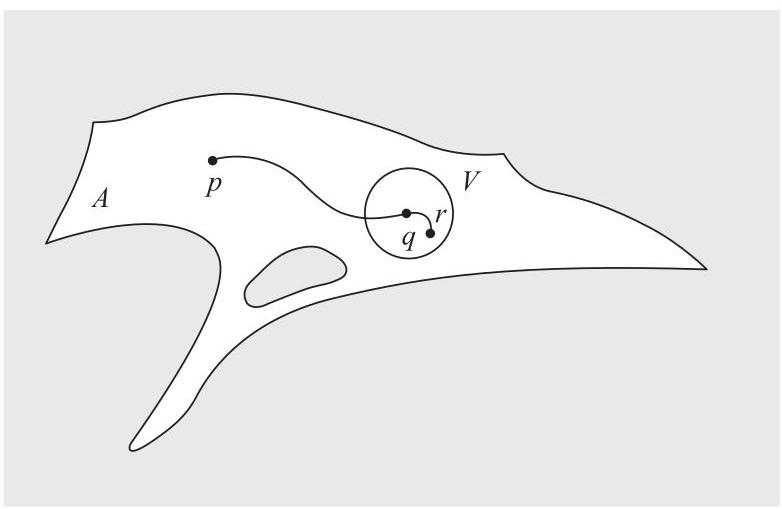
\includegraphics[max width=0.7\textwidth]{images/bo_d4b9jf3ef24c73e0334g_479_376_770_782_509_0.jpg}
\end{center}
\hspace*{3em} 

图 A5-3

通过类似的论证，我们证明了 \({A}_{1}\) 的补集在 \(A\) 中也是开集.因此， \({A}_{1}\) 在 \(A\) 中既是开集又是闭集.由于 \(A\) 是局部弧连通的， \({A}_{1}\) 非空.由于 \(A\) 是连通的， \({A}_{1} = A\) .Q.E.D.

例 4. 一个集合可能是弧连通的，但却不是局部弧连通的.例如，设 \(A \subset  {R}^{2}\) 是由通过 \(\left( {1/n,0}\right) ,n = 1,\ldots\) 的垂直线以及 \(x\) 和 \(y\) 轴组成的集合. \(A\) 显然是弧连通的，但 \(\left( {0,y}\right) ,y \neq  0\) 的一个小邻域不是弧连通的.这是因为虽然连接任意两点 \(p,q \in  A\) 之间存在一条“长”弧，但可能不存在连接这两点的短弧(图 A5-4).

\section*{C. 紧集}

定义 12. 如果一个集合 \(\mathrm{A} \subset  {\mathbb{R}}^{N}\) 包含在 \({\mathbb{R}}^{N}\) 的某个球内，则称 \(\mathrm{A} \subset  {\mathbb{R}}^{N}\) 是有界的.如果一个集合 \(\mathrm{K} \subset  {\mathbb{R}}^{N}\) 是闭集且有界，则称其为紧集.

\begin{center}
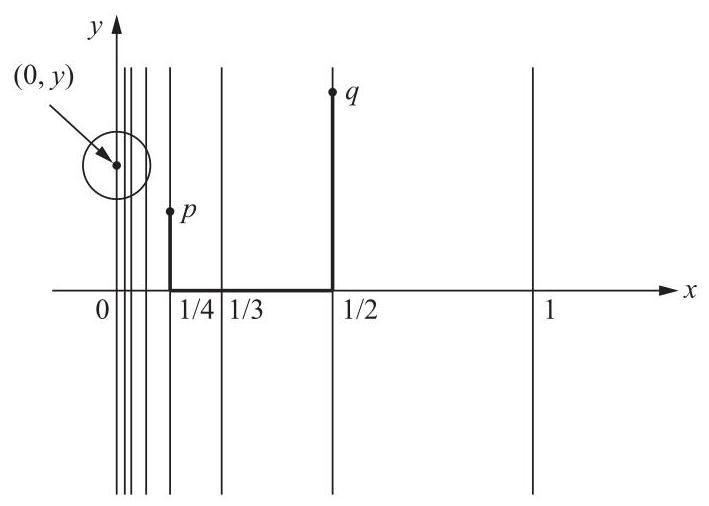
\includegraphics[max width=0.6\textwidth]{images/bo_d4b9jf3ef24c73e0334g_480_428_196_709_506_0.jpg}
\end{center}
\hspace*{3em} 

图 A5-4

我们在第 2-7 节中已经遇到过紧集.为完整起见，我们在此证明紧集的性质 1 和 2，这些性质在第 2-7 节中已被假定.

定义 13. 集合 \(\mathrm{A} \subset  {\mathbb{R}}^{N}\) 的一个开覆盖是开集族 \(\left\{  {\mathrm{U}}_{\alpha }\right\}  ,\alpha  \in  \mathfrak{a}\) ，使得 \(\mathop{\bigcup }\limits_{\alpha }{\mathrm{U}}_{\alpha } \supset  \mathrm{A}\) .当族中只有有限个 \({\mathrm{U}}_{\alpha }\) 时，我们称该覆盖是有限的.如果子族 \(\left\{  {\mathrm{U}}_{\beta }\right\}  ,\beta  \in  \mathfrak{B} \subset  \mathfrak{a}\) 仍然覆盖 \(\mathrm{A}\) ，即 \(\mathop{\bigcup }\limits_{\beta }{\mathrm{U}}_{\beta } \supset  \mathrm{A}\) ，我们称 \(\left\{  {\mathrm{U}}_{\beta }\right\}\) 是 \(\left\{  {\mathrm{U}}_{\alpha }\right\}\) 的子覆盖.

命题 11. 对于集合 \(\mathrm{K} \subset  {\mathbb{R}}^{N}\) ，以下断言是等价的:

1. K 是紧集.

2. (Heine-Borel 定理). \(\mathrm{K}\) 的每个开覆盖都有一个有限子覆盖.

3. (Bolzano-Weierstrass 定理). \(\mathrm{K}\) 的每个无限子集在 \(\mathrm{K}\) 中都有一个极限点.

证明.我们将证明 \(1 \Rightarrow  2 \Rightarrow  3 \Rightarrow  1\) .

\(1 \Rightarrow  2\) :设 \(\left\{  {U}_{\alpha }\right\}  ,\alpha  \in  \mathfrak{a}\) 是紧集 \(K\) 的一个开覆盖，并假设 \(\left\{  {U}_{\alpha }\right\}\) 没有有限子覆盖.我们将证明这会导致矛盾.

由于 \(K\) 是紧集，它包含在一个闭合的矩形区域内

\[
B = \left\{  {\left( {{x}_{1},\ldots ,{x}_{n}}\right)  \in  {R}^{n};{a}_{j} \leq  {x}_{j} \leq  {b}_{j},\;j = 1,\ldots ,n}\right\}  .
\]

我们用超平面 \({x}_{j} = \left( {{a}_{j} + {b}_{j}}\right) /2\) 来划分 \(B\) (例如，如果 \(K \subset  {R}^{2}\) 是一个矩形，我们将 \(B\) 分割成 \({2}^{2} = 4\) 个矩形).因此，我们得到 \({2}^{n}\) 个更小的闭合矩形区域.根据假设，其中至少一个区域，记为 \({B}_{1}\) ，使得 \({B}_{1} \cap  K\) 没有被 \(\left\{  {U}_{\alpha }\right\}\) 中的有限个开集覆盖.我们现在以类似的方式划分 \({B}_{1}\) ，并通过重复这个过程，我们得到一个闭合矩形区域序列 (图 A5-5)

\[
{B}_{1} \supset  {B}_{2} \supset  \cdots  \supset  {B}_{i} \supset  \cdots
\]

\begin{center}
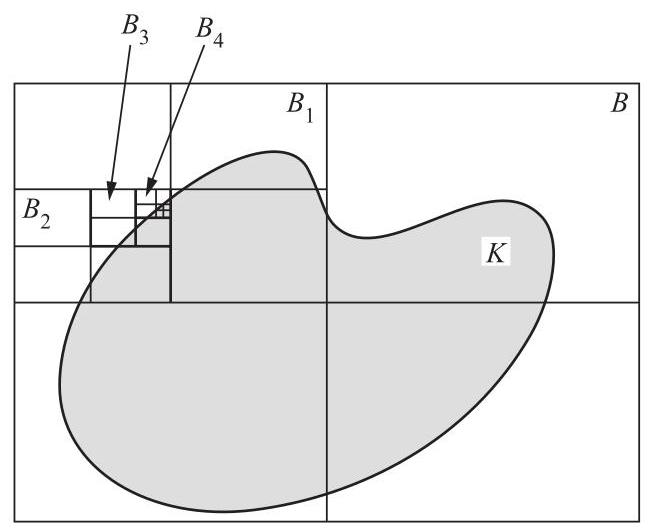
\includegraphics[max width=0.5\textwidth]{images/bo_d4b9jf3ef24c73e0334g_481_440_197_652_531_0.jpg}
\end{center}
\hspace*{3em} 

图 A5-5

使得 \({B}_{i} \cap  K\) 没有被 \(\left\{  {U}_{\alpha }\right\}\) 中的有限个开集覆盖，并且 \({B}_{i}\) 的最大边长收敛于零.

我们声称存在 \(p \in   \cap  {B}_{i}\) .事实上，通过将每个 \({B}_{i}\) 投影到 \({R}^{n},j = l,\ldots ,n\) 的 \(j\) 轴上，我们得到一个闭合区间序列

\[
\left\lbrack  {{a}_{j1},{b}_{j1}}\right\rbrack   \supset  \left\lbrack  {{a}_{j2},{b}_{j2}}\right\rbrack   \supset  \cdots  \supset  \left\lbrack  {{a}_{ji},{b}_{ji}}\right\rbrack   \supset  \cdots .
\]

由于 \(\left( {{b}_{ji} - {a}_{ji}}\right)\) 任意小，我们看到

\[
{a}_{j} = \sup \left\{  {a}_{ji}\right\}   = \inf \left\{  {b}_{ji}\right\}   = {b}_{j};
\]

因此，

\[
{a}_{j} \in  \mathop{\bigcap }\limits_{i}\left\lbrack  {{a}_{ji},{b}_{ji}}\right\rbrack
\]

因此，正如我们所声称的， \(p = \left( {{a}_{1},\ldots ,{a}_{n}}\right)  \in  \mathop{\bigcap }\limits_{i}{B}_{i}\) .

现在， \(p\) 的任何邻域都包含一些 \({B}_{i}\) ，当 \(i\) 足够大时；因此，它包含无限多个 \(K\) 的点.因此， \(p\) 是 \(K\) 的一个极限点，并且由于 \(K\) 是闭集， \(p \in  K\) .设 \({U}_{0}\) 是包含 \(p\) 的族 \(\left\{  {U}_{\alpha }\right\}\) 中的一个元素.由于 \({U}_{0}\) 是开集，存在一个球 \({B}_{\epsilon }\left( p\right)  \subset  {U}_{0}\) .另一方面，当 \(i\) 足够大时， \({B}_{i} \subset  {B}_{\epsilon }\left( p\right)  \subset  {U}_{0}\) .这与任何 \({B}_{i} \cap  K\) 都不能被有限个 \({U}_{\alpha }\) 覆盖的事实相矛盾，并证明了 \(1 \Rightarrow  2\) .

\(2 \Rightarrow  3\) .假设 \(A \subset  K\) 是 \(K\) 的一个无限子集，并且 \(K\) 的没有点是 \(A\) 的极限点.那么，对于每个 \(p \in  K,p \notin  A\) ，可以选择 \(p\) 的一个邻域 \({V}_{p}\) ，使得 \({V}_{p} \cap  A = \phi\) ，并且对于每个 \(q \in  A\) ，可以选择 \(q\) 的一个邻域 \({W}_{q}\) ，使得 \({W}_{q} \cap  A = q\) .因此，族 \(\left\{  {{V}_{p},{W}_{p}}\right\}\) ， \(p \in  K - A,q \in  A\) ，是 \(K\) 的一个开覆盖.由于 \(A\) 是无限的，并且省略该族中的任何一个 \({W}_{q}\) 都会留下未被覆盖的点 \(q\) ，因此族 \(\left\{  {{V}_{p},{W}_{q}}\right\}\) 没有有限子覆盖.这与命题 2 相矛盾.

\(3 \Rightarrow  1\) :我们必须证明 \(K\) 是闭集且有界. \(K\) 是闭集，因为如果 \(p\) 是 \(K\) 的极限点，通过考虑同心球 \({B}_{1/i}\left( p\right)  = \; {B}_{i}\) ，我们得到一个序列 \({p}_{1} \in  {B}_{1} - {B}_{2},{p}_{2} \in  {B}_{2} - {B}_{3},\ldots ,{p}_{i} \in  {B}_{i} - {B}_{i + 1},\ldots\) ，它以 \(p\) 为极限点.根据命题 \(3,p \in  K\) .

\(K\) 是有界的.否则，通过考虑半径为 \(1,2,\ldots ,i,\ldots\) 的同心球 \({B}_{i}\left( p\right)\) ，我们将得到一个没有极限点的序列 \({p}_{1} \in  {B}_{1},{p}_{2} \in  {B}_{2} - {B}_{1},\ldots ,{p}_{i} \in \; {B}_{i} - {B}_{i - 1},\ldots\) .这证明了 \(3 \Rightarrow  1\) .

下一个命题表明紧集的连续像也是紧集.

命题 12.设 \(\mathrm{F} : \mathrm{K} \subset  {\mathbb{R}}^{N} \rightarrow  {\mathbb{R}}^{\mathrm{m}}\) 是连续的，设 \(\mathrm{K}\) 是紧集.则 \(\mathrm{F}\left( \mathrm{K}\right)\) 是紧集.

证明. 若 \(F\left( K\right)\) 有限，则其显然是紧的. 假设 \(F\left( K\right)\) 不是有限的，并考虑一个无限子集 \(\left\{  {F\left( {p}_{\alpha }\right) }\right\}   \subset  F\left( K\right) ,{p}_{\alpha } \in  K\) . 显然集合 \(\left\{  {p}_{\alpha }\right\}   \subset  K\) 是无限的，并且根据紧性，存在一个极限点 \(q \in  K\) . 因此，存在一个序列 \({p}_{1},\ldots ,{p}_{i},\ldots , \rightarrow  q,{p}_{i} \in  \left\{  {p}_{\alpha }\right\}\) . 由于 \(F\) 的连续性，序列 \(F\left( {p}_{i}\right)  \rightarrow  F\left( q\right)  \in  F\left( K\right)\) (命题 1). 因此， \(\left\{  {F\left( {p}_{\alpha }\right) }\right\}\) 有一个极限点 \(F\left( q\right)  \in  F\left( K\right)\) ; 所以， \(F\left( K\right)\) 是紧的.Q.E.D.

以下可能是紧集最重要的性质.

命题 13. 令 \(\mathrm{f} : \mathrm{K} \subset  {\mathbb{R}}^{N} \rightarrow  \mathbb{R}\) 是定义在紧集 \(\mathrm{K}\) 上的连续函数. 则存在 \({\mathrm{p}}_{1},{\mathrm{p}}_{2} \in  \mathrm{K}\) 使得

\[
\mathrm{f}\left( {\mathrm{p}}_{2}\right)  \leq  \mathrm{f}\left( \mathrm{p}\right)  \leq  \mathrm{f}\left( {\mathrm{p}}_{1}\right) \text{ for all }\mathrm{p} \in  \mathrm{K}\text{ ; }
\]

即， \(\mathrm{f}\) 在 \({\mathrm{p}}_{1}\) 处达到最大值，在 \({\mathrm{p}}_{2}\) 处达到最小值.

证明. 我们将证明 \({p}_{1}\) 的存在性；最小值的情况可以类似地处理.

根据命题 12， \(f\left( K\right)\) 是紧的，因此是闭合且有界的. 因此，存在 sup \(f\left( K\right)  = {x}_{1}\) . 由于 \(f\left( K\right)\) 是闭合的， \({x}_{1} \in  f\left( K\right)\) . 因此，存在 \({p}_{1} \in  K\) 使得 \({x}_{1} = f\left( {p}_{1}\right)\) . 显然，对于所有 \(p \in  K\) ，有 \(f\left( p\right)  \leq  f\left( {p}_{1}\right)  = {x}_{1}\) .Q.E.D.

尽管我们不会用到它，但一致连续的概念在当前上下文中如此自然，以至于我们应该对此说几句.

映射 \(F : A \subset  {R}^{n} \rightarrow  {R}^{m}\) 在 \(A\) 上是一致连续的，如果给定 \(\epsilon  > 0\) ，存在 \(\delta  > 0\) 使得对于所有 \(p \in  A\) ，有 \(F\left( {{B}_{\delta }\left( p\right) }\right)  \subset  {B}_{\epsilon }\left( {F\left( p\right) }\right)\) .

形式上，这个定义与(简单)连续的定义之间的区别在于，这里给定 \(\epsilon\) ，数字 \(\delta\) 对于所有 \(p \in  B\) 都是相同的，而在简单连续中，给定 \(\epsilon\) ，数字 \(\delta\) 可能随 \(p\) 而变化. 因此，一致连续是一个全局概念，而不是局部概念.

一个重要事实是，在紧集上，这两种概念是一致的. 更准确地说，令 \(\mathrm{F} : \mathrm{K} \subset  {\mathbb{R}}^{N} \rightarrow  {\mathbb{R}}^{\mathrm{m}}\) 是连续的且 \(\mathrm{K}\) 是紧的. 则 \(\mathrm{F}\) 在 \(\mathrm{K}\) 上是一致连续的.

如果回忆起第 2-7 节中介绍的开覆盖的勒贝格数概念，那么这个事实的证明就很简单.事实上，给定 \(\epsilon  > 0\) ，对于每个 \(p \in  K\) ，都存在一个数 \(\delta \left( p\right)  > 0\) ，使得 \(F\left( {{B}_{\delta \left( p\right) }\left( p\right) }\right)  \subset  {B}_{\epsilon /2}\left( {F\left( p\right) }\right)\) .

族 \(\left\{  {{B}_{\delta \left( p\right) }\left( p\right) ,p \in  K}\right\}\) 是 \(K\) 的一个开覆盖.设 \(\delta  > 0\) 是这个族的勒贝格数(第 2-7 节，性质 3).如果 \(q \in  {B}_{\delta }\left( p\right)\) ， \(p \in  K\) ，那么 \(q\) 和 \(p\) 属于开覆盖的某个元素.因此， \(\left| {F\left( p\right)  - F\left( q\right) }\right|  < \epsilon\) .由于 \(q\) 是任意的， \(F\left( {{B}_{\delta }\left( p\right) }\right)  \subset  {B}_{\epsilon }\left( {F\left( p\right) }\right)\) .这表明 \(\delta\) 满足一致连续的定义，正如我们所期望的.

\section*{D. 连通分支}

当一个集合不连通时，它可以被分成其连通分支.为了使这个想法更精确，我们将首先证明以下命题.

命题 14. 设 \({\mathrm{C}}_{\alpha } \subset  {\mathbb{R}}^{N}\) 是一个连通集合族，使得

\[
\mathop{\bigcap }\limits_{\alpha }{C}_{\alpha } \neq  \phi
\]

则 \(\mathop{\bigcup }\limits_{\alpha }{\mathrm{C}}_{\alpha } = \mathrm{C}\) 是一个连通集合.

证明.假设 \(C = {U}_{1} \cup  {U}_{2}\) ，其中 \({U}_{1}\) 和 \({U}_{2}\) 是非空、不相交的开集，并且某个点 \(p \in  \mathop{\bigcap }\limits_{\alpha }{C}_{\alpha }\) 属于 \({U}_{1}\) .设 \(q \in  {U}_{2}\) .由于 \(C = \mathop{\bigcup }\limits_{\alpha }{C}_{\alpha }\) 和 \(p \in  \mathop{\bigcap }\limits_{\alpha }{C}_{\alpha }\) ，存在某个 \({C}_{\alpha }\) 使得 \(p,q \in  {C}_{\alpha }\) .那么 \({C}_{\alpha } \cap  {U}_{1}\) 和 \({C}_{\alpha } \cap  {U}_{2}\) 是非空、不相交的开集.这与 \({C}_{\alpha }\) 的连通性矛盾，并表明 \(C\) 是连通的.Q.E.D.

定义 14. 设 \(\mathrm{A} \subset  {\mathbb{R}}^{N}\) 和 \(p \in  A\) .包含 \(\mathrm{p}\) 的 A 的所有连通子集的并集称为包含 p 的 A 的连通分支.

根据命题 14，连通分支是一个连通集合.直观上，包含 \(p \in  A\) 的 \(A\) 的连通分支是 \(A\) 的最大连通子集(即，它不包含在包含 \(p\) 的 \(A\) 的任何其他连通子集中).

一个集合 \(A\) 的连通分支在 \(A\) 中总是闭合的.这是以下命题的结果.

命题 15. 设 \(\mathrm{C} \subset  \mathrm{A} \subset  {\mathbb{R}}^{N}\) 是一个连通集合.则 \(\mathrm{C}\) 在 \(\mathrm{A}\) 中的闭包 \(\overline{\mathrm{C}}\) 是连通的.

证明. 假设 \(\bar{C} = {U}_{1} \cup  {U}_{2}\) ，其中 \({U}_{1},{U}_{2}\) 是 \(\bar{C}\) 中的非空、不相交的开集. 因为 \(\bar{C} \supset  C\) ，集合 \(C \cap  {U}_{1} = {V}_{1},C \cap  {U}_{2} = {V}_{2}\) 在 \(C\) 中是开集、不相交的，并且 \({V}_{1} \cup  {V}_{2} = C\) . 我们将证明 \({V}_{1}\) 和 \({V}_{2}\) 是非空的，从而与 \(C\) 的连通性产生矛盾.

设 \(p \in  {U}_{1}\) . 因为 \({U}_{1}\) 在 \(\bar{C}\) 中是开集，存在 \(p\) 在 \(A\) 中的一个邻域 \(W\) ，使得 \(W \cap  \bar{C} \subset  {U}_{1}\) . 因为 \(p\) 是 \(C\) 的一个极限点，存在 \(q \in  W \cap  C \subset \; W \cap  \bar{C} \subset  {U}_{1}\) . 因此， \(q \in  C \cap  {U}_{1} = {V}_{1}\) ，并且 \({V}_{1}\) 非空. 类似地，可以证明 \({V}_{2}\) 非空.Q.E.D.

推论. 集合 \(\mathrm{A}\) 的一个连通分支 \(\mathrm{C} \subset  \mathrm{A} \subset  {\mathbb{R}}^{N}\) 在 A 中是闭集.

事实上，如果 \(\bar{C} \neq  C\) ，则存在 \(A\) 的一个连通子集，即 \(\bar{C}\) ，它真包含 \(C\) . 这与连通分支 \(C\) 的极大性矛盾.

在某些特殊情况下，集合 \(A\) 的一个连通分支也是 \(A\) 中的一个开集.

命题 16. 设 \(\mathrm{C} \subset  \mathrm{A} \subset  {\mathbb{R}}^{N}\) 是局部弧连通集 \(\mathrm{A}\) 的一个连通分支. 则 \(\mathrm{C}\) 在 \(\mathrm{A}\) 中是开集.

证明. 设 \(p \in  C \in  A\) . 因为 \(A\) 是局部弧连通的，存在 \(p\) 在 \(A\) 中的一个弧连通邻域 \(V\) . 根据命题 \(9,V\) 是连通的. 因为 \(C\) 是极大的， \(C \supset  V\) ；因此， \(C\) 在 \(A\) 中是开集.Q.E.D

\section*{E. 闭映射}

此处我们参考 Lima E. 的著作 Fundamental Groups and Covering Spaces，A.K. Peters 出版社，Jonas Gomes 译自葡萄牙语，马萨诸塞州纳蒂克，2003 年，第 201 页.

定义. 设 \(\widetilde{X}\) 和 \(X\) 是拓扑空间， \(f : \widetilde{X} \rightarrow  X\) 是一个映射；当映射 \(f\) 将 \(\widetilde{X}\) 中的闭集映射到 \(X\) 中的闭集时，称该映射为闭映射.

命题. \(f : \widetilde{X} \rightarrow  X\) 为闭映射的充要条件是:给定 \(x \in  X\) 以及 \(\widetilde{X}\) 中的开集 \(\widetilde{U} \supset  {f}^{-1}\left( x\right)\) ，存在 \(X\) 中的开集 \(U\) ，使得 \(x \in  U\) 且 \({f}^{-1}\left( U\right)  \subset  \widetilde{U}\) .

证明.该条件是必要的.因为，如果 \(f\) 是闭集，则 \(f\left( {\widetilde{X} - \widetilde{U}}\right)\) 在 \(X\) 中是闭集.由于它不包含 \(x\) ，存在一个开集 \(U \ni  x\) 使得 \(U \cap  f\left( {\widetilde{X} - \widetilde{U}}\right)  \neq  \varnothing\) .由此可知 \({f}^{-1}\left( U\right)  \subset  \widetilde{U}\) ，这就是命题中的条件.

该条件是充分的.因为如果我们假设该条件，设 \(F \subset  \widetilde{X}\) 是 \(\widetilde{X}\) 中的一个闭集.选择 \(x \notin  f\left( F\right)\) .那么 \(F \cap  {f}^{-1}\left( x\right)  = \varnothing\) .因此开集 \(\widetilde{U} = \left( {X - F}\right)\) 包含 \({f}^{-1}\left( x\right)\) .由此可知存在一个开集 \(U \ni  x\) 使得 \({f}^{-1}\left( U\right)  \subset  \widetilde{U}\) .这表明 \(U \cap  f\left( F\right)  \neq  \varnothing\) ，即 \(f\left( F\right)\) 在 \(X\) 中是闭集.

注记.如果 \({f}^{-1}\) 是一个映射，则命题的条件将说明 \({f}^{-1}\) 是连续的；请注意 \({f}^{-1}\left( x\right)\) 不是 \(X\) 中的一个点，而它通常是一个集合.

参考文献与评论

曲面微分几何的基础性工作是高斯的论文“Disquisitiones generales circa superficies curvas”，Comm. Soc. Göttingen Bd 6, 1823-1827.有多种语言的译本，例如，

1. Gauss, K. F., General Investigations of Curved Surfaces, Raven Press, New York, 1965.

我们相信本书的读者现在已经能够尝试理解那篇论文了.需要耐心和开放的心态，但这种体验将非常有益.

曲面微分几何的经典来源是达布的四卷本著作:

2. Darboux, G., 曲面论，Gauthier-Villars出版社，巴黎，1887年、1889年、1894年、1896年.有Chelsea Publishing Co., Inc.出版社纽约版重印本.

对于初学者来说，这是一本很难读的书.然而，除了丰富的信息外，这本书中仍有许多未探索的思想，使得时不时地翻阅它仍然很有价值.

在英语中最具影响力的经典著作可能是

3. Eisenhart, L. P.，曲线与曲面微分几何学论，Ginn and Company出版社，波士顿，1909年，Dover出版社纽约版重印，1960年.

在经典微分几何的一些直观思想方面，可以在第4章中找到极好的阐述，该章出自

4. Hilbert, D. 和 S. Cohn-Vossen，几何与想象，Chelsea Publishing Company, Inc.出版社，纽约，1962年(德文原书翻译，首次出版于1932年).

下面我们将按时间顺序介绍几本其他教科书.它们的难度或多或少与本书相当.更完整的列表可以在[9]中找到，此外，[9]还包含许多全局定理.

5. Struik, D. J.，经典微分几何讲义，Addison-Wesley出版社，Reading, Mass.，1950年.

6. Pogorelov, A. V.，微分几何，Noordhoff出版社，Groningen, Netherlands，1958年.

7. Willmore, T. J.，微分几何入门，Oxford University Press, Inc.出版社，伦敦，1959年.

8. O'Neill, B.，初等微分几何，Academic Press出版社，纽约，1966年.

9. Stoker, J. J.，微分几何，Wiley-Interscience出版社，纽约，1969年.

本书未涉及的移动标架法的清晰初等阐述可以在[8]中找到.此外，本书简要介绍的曲线理论的更多细节可以在[5]、[6]和[9]中找到.

虽然不是教科书，但以下参考文献也应包含在内.参考文献[10]是对曲线和曲面的一些全局定理的美妙阐述，而[11]是一组成为该主题经典的讲义笔记.

10. Chern, S. S.，欧几里得空间中的曲线与曲面，全局几何与分析研究，MAA数学研究，美国数学家协会，1967年.

11. Hopf, H.，大范围微分几何，数学讲义，第1000号，第二部分，第76-187页，Springer出版社，1989年.

若要进行更深入的阅读，可能需要先学习一些关于可微流形和李群的知识.例如，

12. Spivak, M., A Comprehensive Introduction to Differential Geometry, Vol. 1, Brandeis University, 1970.

13. Warner, F., Foundations of Differentiable Manifolds and Lie Groups, Scott, Foresman, Glenview, Ill., 1971.

参考文献 [12] 是一本愉快的读物. [13] 的第 1-4 章对该主题的基础知识进行了简短而有效的阐述.

之后，可供选择的阅读材料很多，取决于读者的品味和兴趣.下面我们提供一个可能的选择，绝非唯一.在 [17] 和 [18] 中可以找到大量的书籍和论文列表.

14. Berger, M., P. Gauduchon, and E. Mazet, Le Spectre d'une Variété Riemannienne, Lecture Notes 194, Springer, Berlin, 1971.

15. Bishop, R. L., and R. J. Crittenden, Geometry of Manifolds, Academic Press, New York, 1964.

16. Cheeger, J., and D. Ebin, Comparison Theorems in Riemannian Geometry, North-Holland, Amsterdam, 1974.

17. Helgason, S., Differential Geometry and Symmetric Spaces, Academic Press, New York, 1963.

18. Kobayashi, S., and K. Nomizu, Foundations of Differential Geometry, Vols. I and II, Wiley-Interscience, New York, 1963 and 1969,

19. Gromoll, D., Klingenberg, W. and W. Meyer, Riemannsche Geometrie im Grossen, Lecture Notes 55, Springer-Verlag, Berlin, 1968.

20. Lawson, B., Lectures on Minimal Submanifolds, Monografias de Matemática, IMPA, Rio de Janeiro, 1973.

21. Milnor, J., Morse Theory, Princeton University Press, Princeton, N. J., 1963.

22. Spivak, M., A Comprehensive Introduction to Differential Geometry, Vol. I to V, Publish or Perish, Inc., 2005.

\section*{索引}

加速度向量，350

累积点, 461

角度:

两曲面之间, 89

外角, 269

内角, 278

对径映射, 82

弧, 465 正则, 269

弧长, 6

在极坐标中, 26 (例 11)

通过弧长重参数化, 23

面积, 100

几何定义, 117

图的面积, 102 (例 5)

定向面积, 16 (例 10), 168

旋转曲面的面积, 103 (例 11)

保面积微分同胚, 233 (例 18), 234 (例 20)

渐近线，150

渐近方向，150

球，120

Beltrami-Enneper 定理，154 (例 13)

Beltrami 测地映射定理，301 (例 12)

Bertrand 曲线，27

Bertrand 配对曲线，27

副法线，20

副法向量，18

Bolzano-Weierstrass 定理，115, 126, 469

Bonnet, O., 268

Bonnet 定理，358, 429

集合的边界，463

Braunmühl, A., 369

Buck, R. C., 45, 100, 133

Calabi, E., 359

悬链线, 25 (例 8)

悬链面, 224

渐近线, 170 (例 3)

与螺旋面局部等距, 216 (例 14), 226

作为极小曲面, 204

Cauchy-Crofton公式, 42

Cauchy序列, 464

在内禀距离中, 342 (例 5)

链式法则, 93 (例 24), 127, 131

陈省身, S. S., 323

与Lashof, R., 393

Christoffel符号, 235

在法坐标中, 299 (例 4)

对于旋转曲面, 236

Diocles的弦曲线, 7 (例 3)

Clairaut关系, 260

闭合平面曲线，32

闭集，462

集合的闭包，462

紧集，114, 468

比较定理，374 (例 3)

相容性方程，239

完备曲面，331

锥面，66, 67 (例 3), 333

其测地线，312 (例 6)

其与平面之间的局部等距，226

作为直纹曲面，192

共形映射，229

线性，232 (例 13)

局部，229, 233 (例 14)

平面之间的，233 (例 15)

球面到平面的，233 (例 16)

共轭方向，152

共轭轨迹，368

共轭极小曲面，216 (例 14)

共轭点，368

Kneser 关于的判据，376 (例 7)

连通，465

弧状连通，465

局部连通，467

连通分量，472

单局部连通，389

联络，311 (例 2), 447

锥面，213 (例 5)

曲线的接触，173 (例 9)

曲线与曲面的接触，174 (例 10)

曲面的接触，94 (例 27), 172 (例 8)

连续映射，122

均匀地, 471

收敛, 460

内禀距离, 341 (例 4)

凸曲线, 39

凸包, 50 (例 11)

凸邻域, 307

存在性, 309

凸集, 50 (例 9)

凸性和曲率, 41, 177 (例 24), 393, 403

坐标曲线, 55

坐标邻域, 55

坐标系, 55

Courant, R., 117

协变导数, 241

代数值, 251

沿曲线, 243

的表达式, 242

的性质, 310 (Ex. 2)

用平行移动表示, 310 (Ex. 1)

覆盖空间, 377

的片数, 384

可定向双层, 449 (Exs. 3, 4)

临界点, 60, 92 (Ex. 13)

非退化, 177 (Ex. 23)

临界值, 60

叉积, 13

曲率:

高斯曲率, 148, 158 (参见高斯曲率)

测地曲率, 251, 256

曲率线, 147 的微分方程, 163

平均曲率, 148, 158, 166

向量曲率, 203

普通, 143

平面曲线的, 22

主, 146

的半径, 20

截面, 448

空间曲线的, 17

在任意参数中, 26 (例 12)

曲线:

渐近的, 150

的微分方程, 162

极大的, 417

\({C}^{k},{10}\) 类的 (例 7)

闭合的, 32

连续的, 399

分段正则的, 269

单的, 32

坐标, 55

发散, 342 (例 7)

打结的, 409

水平, 104 (例 14)

参数化的, 3

分段可微, 334

分段正则, 247

正则, 6

分段 \({C}^{1},{37}\)

简单, 10 (例 7)

切痕, 425

摆线, 7

圆柱体, 67 (例 1)

第一基本形式, 96

等距变换, 232 (例 12)

局部等距变换, 与平面, 222

正常截面，146

作为一条规则曲面，192

达布三面体，264 (例 14)

映射的次数，397

可展曲面，197, 213 (例 3)

分类，197

作为切平面族包络，198

切平面，213 (例 6)

微分同胚，76

保面积的，233 (例 18, 19)

局部，89 保向的，168 反向的，168

可微函数，75, 83 (例 9), 84 (例 13), 126

可微流形，444

可微映射，75, 128, 432

可微结构，431, 444

映射的微分，89, 128

方向:

渐近的, 150

主, 146

方向:共轭, 152

场, 181

直纹曲面的准线, 191

曲面上的距离, 335

分布参数, 195

do Carmo, M. 和 E. Lima, 394

定义域, 99

点积, 4

Dupin 指示曲面, 150

的几何解释, 166

Dupin 关于三正交系的定理, 155

三角剖分边, 275

Efimov, N. V., 457

特征值, 219

特征向量, 219

椭球, 63, 82 (例 4), 93 (例 20)

共轭轨迹, 266

第一基本形式, 102 (例 1)

高斯曲率, 176 (例 21)

参数化, 69 (例 12)

脐点, 175

嵌入, 441

克莱因瓶到 \({\mathbb{R}}^{4},{442}\) 的嵌入

射影平面到 \({\mathbb{R}}^{4},{443}\) 的嵌入

环面到 \({\mathbb{R}}^{4},{441}\) 的嵌入

曲线的能量, 311 (例 4)

Enneper 曲面, 170 (例 3)

作为极小曲面, 208

切平面族包络, 198, 213 (例 8), 215 (例 10), 247, 313 (例 7)

欧几里得第五公理, 283, 436, 438

欧拉公式, 147

欧拉-拉格朗日方程, 371

欧拉-庞加莱示性数, 275

渐屈线, 24 (例 7)

指数映射, 288

其可微性, 289

三角剖分的面, 275

Fary-Milnor 定理, 409

Fenchel 定理, 405

费米坐标, 311 (例 3)

方向场, 181

其微分方程, 182

其积分曲线, 182

单位法向量场, 107

第一基本形式, 94

平面环面, 440

焦点曲面, 214 (例 9)

笛卡尔叶形线, 9 (例 5)

弗勒内公式, 20

弗勒内三面体, 20

函数:

解析的, 209

分量, 122

连续的, 121

可微的, 75, 126

调和的, 204

高度, 75

莫尔斯, 177 (例 23)

曲线局部理论基本定理, 20, 315

曲面局部理论基本定理, 239, 317

高斯-博内定理 (整体), 277 应用, 280

高斯-博内定理(局部)，272

高斯公式，238

正交坐标系中的，240(例 1)

高斯引理，292

高斯映射，138

高斯曲率绝妙定理，237

高斯曲率，148, 158

的几何解释，168

可微函数图像的，166

平行移动的，274

曲面亏格，276

测地线:

圆，291

坐标，311(例 3)

曲率，251, 256

流，446

映射，300 (例 11)

平行线，311 (例 3)

测地线:(续)

极坐标，290

第一基本形式，291

高斯曲率，292

测地线，300 (例 7)

挠率，155 (例 19)，264 (例 14)

测地线，312

圆锥的，312 (例 6)

圆柱的，249, 250

微分方程，257

存在性，257

极小，307, 337

极小性质，296

旋转抛物面的，261-262

庞加莱半平面, 437, 438, 450 (例 8)

径向, 291

作为变分问题的解, 351

球面, 249

旋转曲面, 258-261, 362 (例 5)

Gluck, H., 42

曲面上的梯度, 104 (例 14)

可微函数的图像, 60

面积, 102 (例 5)

高斯曲率, 166

平均曲率, 166

第二基本形式, 166

切平面, 90 (例 3)

Green, L., 369

Gromov, M. L., and V. A. Rokhlin, 457

等距群, 232 (例 9)

Hadamard 关于 K ≤ O 的完备曲面定理, 393, 396 (例 9)

Hadamard 关于卵形曲面定理, 393

Hartman, P. 和 L. Nirenberg, 414

Heine-Borel 定理, 115, 126

螺旋面, 96

渐屈线, 170 (例 2)

分布参数, 212 (例 1)

广义, 103 (例 13), 189 (例 6)

曲率线, 212 (例 1)

曲率线, 170 (例 2)

局部等距性, 与悬链面, 216 (例 14), 226

作为极小曲面, 206

作为唯一的极小直纹曲面, 207

切平面, 91 (例 9)

螺旋线, 2, 23 (例 1)

广义, 27 (例 17)

Hessian, 166, 176 (Ex. 22)

Hilbert, D., 451

Hilbert 定理, 451

Holmgren, E., 451

Holonomy 群, 302 (Ex. 13)

Homeomorphism, 125

Homotopic 弧, 385

Homotopy of arcs, 385

free, 396 (Ex. 10)

lifting of, 385

Hopf, H. and W. Rinow, 331, 359

Hopf-Rinow 定理, 338

Hopf 曲面定理 ( \(\mathrm{H} =\) const.), 237 (Ex. 4)

Hurewicz, W., 180

双曲抛物面 (鞍形曲面), 69 (Ex. 11), 图 3-7

双曲抛物面的渐近线, 187

第一基本形式, 102 (例 1)

高斯映射, 141

参数化, 69 (例 11)

作为直纹曲面, 196

双曲平面, 436

单叶双曲面, 90 (例 2), 图 3-34

高斯映射, 153 (例 8)

作为直纹曲面, 193, 212 (例 2)

双叶双曲面, 63

第一基本形式, 102 (例 1)

参数化, 69 (例 13), 102 (例 1)

浸入, 438

等距的, 438

测地线的指标形式, 427

向量场的指标, 283

下确界 (g.l.b.), 464

积分曲线, 182

介值定理, 126

内蕴距离, 228, 335

内蕴几何学, 220, 238, 241

反函数定理, 133

反演, 123

等距同构, 221

线性, 231 (例 7)

局部, 222

在局部坐标系下, 223, 231 (例 2)

切面到平面的, 231 (例 6)

等周不等式, 34

对于测地圆, 300 (例 9)

等温坐标, 204, 230

对于极小曲面, 216 (例 13(b))

雅可比方程, 364

雅可比场，363

球面上的，368

雅可比行列式，130

雅可比矩阵，130

雅可比关于法曲率指示线的定理，281

雅可比关于共轭点的定理，424, 428

Joachimstahl 定理，154 (例 15)

若尔当曲线定理，400

Kazdan, J. 和 F. Warner，451

克莱因瓶，433

嵌入到 \({\mathbb{R}}^{4},{442},{443}\)

的不可定向性，442

Klingenberg 引理，395 (例 8)

Kneser 关于共轭点的判据，376 (例 7)

纽结曲线，409

Lashof, R. 和 S. S. Chern，393

勒贝格数，115

列维-奇维塔联络，447

提升:

弧的提升，382

同伦的提升，385

性质，弧的，386

利马，E. 和 M. do Carmo，394

极限点，461

序列的极限，460

曲率线，147

刘维尔:公式，256

刘维尔曲面，266

曲线的局部正则形式，28

局部凸，177 (例 24), 393 严格局部凸，177 (例 24)

对数螺线，9

球面上的等角线，99, 233

Mainardi-Codazzi 方程, 238

Mangoldt, H., 369

映射:

对径, 82 (例 1)

保形, 229 线性, 232 (例 13)

连续, 122

覆盖, 377

可微, 75, 128, 432

保持距离, 232 (例 8)

指数, 287

高斯, 138

测地线, 300 (例 11)

自伴线性, 217

Massey, W., 414

平均曲率, 148, 158, 166

平均曲率向量, 203

墨卡托投影，233 (例 16)，234 (例 20)

经线，79

Meusnier 定理，144

Milnor, T. Klotz, 457

Minding 定理，292

极小曲面，200

共轭，216 (例 14)

极小曲面的高斯映射，216 (例 13)

极小曲面上的等温参数，204, 216 (例 13(b))

旋转曲面，205

直纹曲面，207

作为变分问题的解，202

莫比乌斯带，108

莫比乌斯带的高斯曲率，175 (例 18)

无穷，448 (例 2)

莫比乌斯带的不可定向性，110, 112 (例 1, 7)

参数化, 108

猴子鞍, 161, 174 (例 11)

莫尔斯指数定理, 427

邻域, 121, 124

凸的, 307

坐标, 55

特殊的, 378

法向, 289

Nirenberg, L. 和 P. Hartman, 414

向量的范数, 4

法向:

坐标, 290

曲率, 143

指示曲面, 281

直线, 89

曲线的法平面, 20

主元，20

截面，144

曲线的向量，18

曲面的向量，89

Olinde Rodrigues，定理，147

开集，120

方向:

曲线的方向变化，7

曲线的方向，112 (例 6)

正方向， \({\mathbb{R}}^{N},{12}\) 的

曲面的方向，106, 138

向量空间的方向，12

定向:

\({\mathbb{R}}^{2},{16}\) 中的定向面积 (例 10)

正定向，简单区域的边界，271

正定向，简单闭合平面曲线，33

定向:(续)

曲面，106, 109

体积在 \({\mathbb{R}}^{3},{17}\) (例 11)

正交:

曲线族，105 (例 15), 184, 189 (例 6)

方向场，184, 188 (例 4), 188 (例 5)

参数化，98, 186

投影，82 (例 2), 123

变换，24 (例 6), 231 (例 7)

密切:

曲线的圆，31 (例 2b)

曲面的抛物面，173 (例 8(c))

曲线的平面，18, 30, 31 (例 1), 31 (例 2)

曲线的球面，174 (例 10(c))

Osserman 定理，211, 343 (例 11)

卵形面，328, 393

旋转抛物面, 82 (例 3)

共轭点, 374 (例 2)

高斯映射, 142

测地线, 261

平行:

曲线, 49 (例 6)

曲面, 215 (例 11)

传递, 245

存在性与唯一性, 245, 255

几何构造, 247

向量场, 244

平行线: 测地线, 311 (例 3(d))

旋转曲面的, 79

参数:

曲线的, 4

分布, 195

参数:

变化，对于曲线，85 (例 15)

变化，对于曲面，72

等温，230

存在性，230

存在性，对于极小曲面，216 (例 13(b))

曲面参数化，55

渐近线参数化，187

曲率线参数化，188

正交，98 存在性，186

划分，10 (例 8), 116

平面:

双曲，436

法，20

密切，18, 30, 31 (例 1), 31 (例 2)

实射影，433

校正, 20

切线, 86

平面, 单参数族切线, 215 (例 10), 313 (例 7)

普拉托问题, 203

庞加莱半平面, 437

完备性, 450 (例 7)

测地线, 438, 450 (例 8)

庞加莱向量场指标定理, 286

点:聚点, 461

中心, 194

共轭, 368

临界, 60, 92 (例 13)

椭圆, 148

双曲, 148

孤立, 464

极限, 461

抛物线, 148

脐带, 149

极, 396 (例 11)

主:

曲率, 146

方向, 146

法向, 20

乘积:

叉乘, 13

点乘, 4

内积, 4

向量, 13

投影, 82 (例 2), 123

墨卡托, 233 (例 16), 234 (例 20)

立体投影, 69 (例 16), 231 (例 4)

射影平面, 433

嵌入 \({\mathbb{R}}^{4},{443}\)

不可定向性, 441

可定向双覆盖, 449 (例 3)

伪球面, 171 (例 6)

曲率半径, 20

射线, 342 (例 6)

法平面, 20

包络, 314 (例 7(b))

区域, 99

有界的, 99

正则, 275

单叶, 271

正则:

曲线, 70 (例 17), 77

参数化曲线, 6

参数化曲面, 80

表面, 54

值, 60,

94 (Ex. 28)

反像, 61, 94 (例 28)

弧长重参数化, 23

黎曼:

流形, 446

上的协变导数, 447

度量, 446 在抽象表面上, 435

结构, 447

刚性运动, 24 (例 6), 44

球体的刚性, 323

Rinow, W. 和 H. Hopf, 331, 359

Rokhlin, V. A. 和 M. L. Gromov, 457

旋转, 77, 88

旋转轴, 79

曲线的旋转指数, 39, 399

有理曲面，191

中心点，194

准线，191

分布参数，195

高斯曲率，195

约束线，194

非柱面，193

生成线，191

生成线，191

Samelson, H., 116

Santaló, L., 47

Scherk 极小曲面，210

Schneider, R., 56

Schur 平面曲线定理，412 (例 7)，413 (例 8)

第二基本形式，143

集合:弧连通，465

有界的, 114

闭合的, 462

紧致的, 114, 468

连通的, 465

凸的, 50 (Ex. 9)

局部单连通, 389

开的, 120

单连通, 388

相似性, 301 (Ex. 11)

相似变换, 190 (Ex. 9), 232 (Ex. 13)

单区域, 271

奇异点:参数化曲线的, 6

参数化曲面的, 80

向量场的, 283

光滑函数, 2

肥皂膜, 202

球面, 57

共轭轨迹, 368-369

作为射影平面的双覆盖, 448 (Ex. 2)

第一基本形式, 98

高斯映射, 139

测地线, 249

等距变换, 232 (Ex. 11), 267 (Ex. 23)

等温参数, 231 (Ex. 4)

雅可比场, 368

可定向性, 106

参数化, 57-60, 69 (Ex. 16)

刚性, 323

球极投影, 69 (Ex. 16)

球面像, 153 (Ex. 9), 283

球极投影, 69 (Ex. 16), 231 (Ex. 4)

Stoker, J. J., 393, 414

Stoker 关于 Efimov 定理的注记，457 (例 1)

Stoker 的平面曲线定理，413 (例 8)

约束线，194

Sturm 振动定理，376 (例 6)

上确界 (l.u.b.)，464

曲面:

抽象的，431

完备的，331

连通的，63

可展的，197, 213 (例 3)

焦面的，214 (例 9)

几何的，435

Liouville 的，266

极小的，200

参数化的，80 正则的，50

正则的，54

旋转曲面(见旋转曲面)

刚性，323

直纹(见直纹曲面)

切线，81

旋转曲面，79

面积，103(例11)

面积保持映射，234(例20)

克里斯托费尔符号，236

共形映射，234(例20)

曲率恒定的，171(例7)，326

延拓的，80

高斯曲率，164

旋转曲面(续)

测地线，258-261

等距映射，232(例10)

平均曲率，165

参数化, 79

主曲率, 165

对称性, 77, 123

Synge引理, 396 (Ex. 10)

切线:

丛, 444

指示线, 24 (Ex. 3), 37

切线到曲线, 6

曲线的切线映射, 399

切平面, 86, 90 (Exs. 1, 3) 抽象曲面的, 435

强切线, 10 (Ex. 7)

切面, 81

切向量到抽象曲面, 433

切向量到曲线, 2

切向量到正则曲面, 85

弱切线, 10 (Ex. 7)

切线，转折定理，270, 402

切比雪夫网，102 (例 3, 4), 240 (例 5), 452

蒂索定理，190 (例 9)

曲面的拓扑性质，275

挠率:

在任意参数化中，26 (例 12)

测地线，155 (例 19), 264 (例 14)

在弧长参数化中，26 (例 12)

符号，29

环面，64

抽象的，439

面积，101

平坦的，440

高斯曲率，159

隐式方程，65

作为克莱因瓶的可定向双覆盖，449 (例 3)

参数化, 67

总曲率, 405

参数化曲线的迹, 2

参数化曲面的迹, 80

牵引线, 8 (例 4)

平移, 24 (例 6)

横截相交, 93 (例 17)

曲面上的三角形, 275

测地线, 267, 282 小的自由移动, 300 (例 8)

三角剖分, 275

三面体:

达布三面体, 264 (例 14)

弗勒内三面体, 20

管状:

邻域, 112, 406

曲面, 91 (例 10), 406

脐点，149

一致连续映射，471

单位法向量，89

变分:

弧长的一阶变分，350

弧长的二阶变分，357

简单测地线的能量二阶变分，312 (例 5)

变分:

断裂变分，426

变分法，360-362 (例 4, 5)

曲线的变分，345

正交变分，351

真变分，345

简单测地线的变分，312

曲面的变分，200

向量:

加速度, 350

长度, 4

范数, 4

切向量 (参见 向量切线)

速度, 2

曲线上的向量场, 243

协变导数, 243

平行, 244

变分, 344

映射上的向量场, 348

平面上的向量场, 178

局部第一积分, 181

局部流, 180

轨迹, 179

曲面上的向量场, 183, 241

协变导数, 241

函数关于某变量的导数，189(例7)

极大轨迹，190(例11)

奇点，283

顶点:四顶点定理，39

平面曲线的，39

分段正则曲线的顶点，269

三角剖分顶点，275

Warner, F. 和 J. Kazdan，451

Weingarten方程，157

绕数，399

\section*{曲线与曲面的微分几何}

修订与更新的第二版

MANFREDO P. DO CARMO

本书是其领域内最广泛使用的教材之一，从局部和整体两个方面介绍了曲线和曲面的微分几何.其表述方式不同于传统方法，更多地使用了初等线性代数，并侧重于基本的几何事实而非技巧或零散的细节.大量的例子和习题，以及部分问题的提示和答案，增强了清晰、写得好的阐述.

内容从曲线章节开始，随后探讨了正则曲面、高斯映射的几何、曲面的内蕴几何以及整体微分几何.本书适合高年级本科生和研究生，先修课程要求包括线性代数本科课程以及对多元微积分的一些熟悉.在此第二版中，作者对全书进行了修正、修订和更新.

Dover修订并更新了1976年由Prentice-Hall, Inc., Englewood Cliffs, New Jersey首次出版的版本.

29.95美元 美国 美国印刷

9 806
\end{document}